\documentclass[
	% -- opções da classe memoir --
	12pt,					% tamanho da fonte
^	openright,			% capítulos começam em pág ímpar (insere página vazia caso preciso)
	oneside,			% para impressão em verso e anverso. Oposto a oneside
	a4paper,			% tamanho do papel. 
	final,				% Use "draft" para compilar mais rápido e "final" para a versão final.
	% -- opções da classe abntex2 --
	%chapter=TITLE,		% títulos de capítulos convertidos em letras maiúsculas
	%section=TITLE,		% títulos de seções convertidos em letras maiúsculas
	%subsection=TITLE,	% títulos de subseções convertidos em letras maiúsculas
	%subsubsection=TITLE,% títulos de subsubseções convertidos em letras maiúsculas
	% -- opções do pacote babel --
	english,				% idioma adicional para hifenização
	french,				% idioma adicional para hifenização
	spanish,			% idioma adicional para hifenização
	brazil				% o último idioma é o principal do documento
	]{abntex2}
\usepackage{lmodern}			% Usa a fonte Latin Modern			
\usepackage[LGR,T1]{fontenc}		% Selecao de codigos de fonte.
\usepackage[utf8]{inputenc}	% Codificacao do documento (conversão automática dos acentos)
\usepackage{lastpage}			% Usado pela Ficha catalográfica
\usepackage{indentfirst}		% Indenta o primeiro parágrafo de cada seção.
\usepackage{color}				% Controle das cores
\usepackage{graphicx}			% Inclusão de gráficos
\usepackage{microtype} 		% Para melhorias de justificação
\usepackage{longtable}		% Usado com "tabu" para criar tabelas em múltiplas páginas
\usepackage{tabu}				% Usado com "longtable" para criar tabelas em múltiplas páginas
\usepackage{array}				% Usado para alguns alinhamentos de células em tabelas
\usepackage{multirow}			% Mescla linhas em tabelas
\usepackage{rotating}			% Gira itens
\usepackage{booktabs}
\usepackage{verse}
% \usepackage{subfig}
\usepackage{caption}
\usepackage{subcaption}
\usepackage{float}
\usepackage{rotfloat}
\usepackage{pdflscape}		% Gira a página para layout "paisagem"
\usepackage{makeidx}			% Cria o índice no final
% \usepackage{multind}			% Cria índices múltiplos no final
% \usepackage{bibtopic}		% Separa a bibliografia por tópicos
% \usepackage[style=abnt,backend=biber]{biblatex}
\usepackage{nomencl} 			% Lista de simbolos
\usepackage{UFBA}
\usepackage{afterpage}
\usepackage{changepage}

% ---
% Pacotes adicionais, usados apenas no âmbito do Modelo Canônico do abnteX2
% ---
\usepackage{lipsum}				% para geração de dummy text
% ---

% ---
% Pacotes de citações
% ---
 \usepackage[brazilian,hyperpageref]{backref}	 % Paginas com as citações na bibl
 \usepackage[alf,abnt-full-initials=yes,abnt-repeated-author-omit=yes,abnt-emphasize=bf,abnt-missing-year=sd]{abntex2cite}	% Citações padrão ABNT

% ---
% Pacote para alinhar itens numerados e sem número igualmente no índice
% ---
% \usepackage[toctextentriesindented]{tocstyle}
% \usetocstyle{nopagecolumn}
% \selecttocstyleoption{tocflat}

% --- 
% CONFIGURAÇÕES DE PACOTES
% --- 

% ---
% Configurações do pacote backref
% Usado sem a opção hyperpageref de backref
 \renewcommand{\backrefpagesname}{Citado na(s) página(s):~}
% Texto padrão antes do número das páginas
\renewcommand{\backref}{}
% Define os textos da citação
 \renewcommand*{\backrefalt}[4]{
	\ifcase #1 %
		Nenhuma citação no texto.%
	\or
		Citado na página #2.%
	\else
		Citado #1 vezes nas páginas #2.%
	\fi}%
\newcommand{\textgreek}[1]{\begingroup\fontencoding{LGR}\selectfont#1\endgroup}
% ---

% ---
% Configurações do pacote ferse
\newcommand{\attrib}[1]{%
\nopagebreak{\raggedleft\footnotesize #1\par}}
\renewcommand{\poemtitlefont}{\normalfont\large\itshape\centering}
% ---

% --- 
% Ambiente A3 Paisagem (insere páginas A3 em modo paisagem ("deitado") no meio do documento)
% ---
\newenvironment{a3paisagem} % ambiente personalizado para inserir uma página A3 no meio de um documento com páginas em tamanho A4
  {\clearpage % começa o processo em página nova
   \pdfpagewidth=2\pdfpagewidth % dobra a largura da página
   \changetext{}{210mm}{}{}{}} % adiciona 210mm à largura da página
  {\clearpage % abre nova página para encerrar o processo
   } % fecha o ambiente e retorna ao tamanho A4
% ---


% ---
% Informações de dados para CAPA e FOLHA DE ROSTO
% ---
\titulo{O distrito soteropolitano de Brotas na Primeira República (1889-1930): conflitos sociais na produção, apropriação e uso do seu espaço urbano}
\autor{Manoel Maria do Nascimento Júnior}
\local{Salvador}
\data{2019}
\orientadora{Odete Dourado}
\coorientadora{Any Brito Leal Ivo}
\instituicao{Universidade Federal da Bahia}
\faculdade{Faculdade de Arquitetura}
\programa{Programa de Pós-Graduação em Arquitetura e Urbanismo}
\tipotrabalho{Dissertação (Mestrado)}
% O preambulo deve conter o tipo do trabalho, o objetivo, 
% o nome da instituição e a área de concentração 
\preambulo{Dissertação apresentada ao Programa de Pós-Graduação em Arquitetura e Urbanismo da Faculdade de Arquitetura da UFBA como requisito parcial para obtenção do grau de Mestre em Arquitetura e Urbanismo}
% ---


% ---
% Configurações de aparência do PDF final

% alterando o aspecto da cor azul
\definecolor{blue}{RGB}{41,5,195}

% informações do PDF
\makeatletter
\hypersetup{
     	%pagebackref=true,
		pdftitle={\@title}, 
		pdfauthor={\@author},
    		pdfsubject={\imprimirpreambulo},
	    pdfcreator={LaTeX with abnTeX2},
		pdfkeywords={urbanismo}{Salvador}{República Velha}{Brotas}{conflitos sociais}, 
		colorlinks=true,       		% false: boxed links; true: colored links
    	linkcolor=blue,          	% color of internal links
    	citecolor=blue,        		% color of links to bibliography
    	filecolor=magenta,      		% color of file links
		urlcolor=blue,
		bookmarksdepth=4,
		breaklinks = true
}
\makeatother
% --- 

% --- 
% Espaçamentos entre linhas e parágrafos 
% --- 

% O tamanho do parágrafo é dado por:
\setlength{\parindent}{1.3cm}

% Controle do espaçamento entre um parágrafo e outro:
\setlength{\parskip}{0.2cm}  % tente também \onelineskip

% ---
% compila o indice
% ---
\makeindex
% ---

% ---
% Configurações de arquivos de imagem
% ---
\DeclareGraphicsExtensions{.pdf, .png, .jpg, .gif, .tif, .tiff, .jpeg}
% ---

% ----
% Início do documento
% ----


\begin{document}

% Retira espaço extra obsoleto entre as frases.
\frenchspacing 

% ----------------------------------------------------------
% ELEMENTOS PRÉ-TEXTUAIS
% ----------------------------------------------------------
\pretextual

% ---
% Capa
% ---
\imprimircapa
% ---

% ---
% Folha de rosto
% (o * indica que haverá a ficha bibliográfica)
% ---
\imprimirfolhaderosto*
% ---

% ---
% Inserir a ficha bibliografica
% ---

% Isto é um exemplo de Ficha Catalográfica, ou ``Dados internacionais de
% catalogação-na-publicação''. Você pode utilizar este modelo como referência. 
% Porém, provavelmente a biblioteca da sua universidade lhe fornecerá um PDF
% com a ficha catalográfica definitiva após a defesa do trabalho. Quando estiver
% com o documento, salve-o como PDF no diretório do seu projeto e substitua todo
% o conteúdo de implementação deste arquivo pelo comando abaixo:
%
% \begin{fichacatalografica}
%     \includepdf{fig_ficha_catalografica.pdf}
% \end{fichacatalografica}
\begin{fichacatalografica}
	\vspace*{\fill}					% Posição vertical
\centering Ficha catalográfica elaborada pelo Sistema Universitário de Bibliotecas (SIBI/UFBA), \\ com os dados fornecidos pelo autor.

	\hrule							% Linha horizontal
N244d
	\begin{center}					% Minipage Centralizado
	\begin{minipage}[c]{12.5cm}		% Largura
	
	Nascimento Júnior, Manoel Maria do % \imprimirautor
	
	\hspace{0.5cm} \imprimirtitulo  / Nascimento Júnior, Manoel Maria do %\imprimirautor%
	. -- \imprimirlocal, \imprimirdata .
	
	\hspace{0.5cm} \pageref{LastPage} p. : il. (algumas color.) ; 30 cm.\\
	
	\hspace{0.5cm} \imprimirorientadoraRotulo~\imprimirorientadora\\
	
	\hspace{0.5cm} \imprimircoorientadoraRotulo~\imprimircoorientadora\\
	
	\hspace{0.5cm}
	\parbox[t]{\textwidth}{\imprimirtipotrabalho~--~\imprimirinstituicao,
	\imprimirdata.}\\
	
	\hspace{0.5cm}
		1. Conflitos sociais.
		2. Urbanização.
		3. Brotas (distrito de Salvador, Bahia).
		4. Primeira República brasileira (1889-1930).
		I. \imprimirorientadoraRotulo~\imprimirorientadora.
		II. \imprimircoorientadoraRotulo~\imprimircoorientadora.
		III. \imprimirinstituicao.
		IV. \imprimirfaculdade.
		V. Título.\\ 			
	
	\hspace{7cm} CDU: 316.482.3:911.375.124(813.8)\\
	\hspace{7cm} CDD: 307.76098142\\
	
	\end{minipage}
	\end{center}
	\hrule
\end{fichacatalografica}
% ---
% ---
% Inserir folha de aprovação
% ---

% Isto é um exemplo de Folha de aprovação, elemento obrigatório da NBR
% 14724/2011 (seção 4.2.1.3). Você pode utilizar este modelo até a aprovação
% do trabalho. Após isso, substitua todo o conteúdo deste arquivo por uma
% imagem da página assinada pela banca com o comando abaixo:
%
% \includepdf{folhadeaprovacao_final.pdf}
%
\begin{folhadeaprovacao}

  \begin{center}
      \MakeUppercase{\ABNTEXchapterfont\bfseries\large\imprimirautor}
    \vspace{1cm}
    
    \MakeUppercase{\ABNTEXchapterfont\Large\imprimirtitulo}
  \end{center}

    \vspace{1cm}  
    \vspace*{\fill}
    \imprimirpreambulo .
    \vspace*{\fill}
            
   \begin{flushright}
     Aprovada em 31 de outubro de 2019
   \end{flushright}
    \vspace{1cm}
   \center\bfseries{Banca Examinadora}

   \assinatura{Dra. \imprimirorientadora \\ Orientadora} 
   \assinatura{Dra. \imprimircoorientadora \\ Co-orientadora } 
   \assinatura{Dr. Fábio Macedo Velame \\ Univ. Federal da Bahia}
   \assinatura{Dra. Carolina Fialho Silva\\ Univ. Federal do Recôncavo da Bahia}
   %\assinatura{\textbf{Professor} \\ Convidado 3}
   %\assinatura{\textbf{Professor} \\ Convidado 4}
      
    \vspace*{2cm}
\end{folhadeaprovacao}
% ---
% ---
% Dedicatória
% ---
\begin{dedicatoria}
   \vspace*{\fill}
   \centering
   \noindent
   \textit{À multidão de trabalhadores anônimos que produziu e produz a cidade do Salvador \\ a cada dia, do jeito que dá, e sobrevive.} \vspace*{\fill}
\end{dedicatoria}
% ---
% ---
% Agradecimentos
% ---
\begin{agradecimentos}
Numa pesquisa com apoio de instituições de fomento, os contribuintes e apoiadores são um vasto universo de pessoas anônimas, sequer sabedoras dos caminhos e descaminhos da investigação feita. Já numa pesquisa feita sem qualquer apoio de instituições de fomento à pesquisa, como a que se inicia com esta dissertação, os contribuintes e apoiadores são muito mais próximos, e cada pequeno gesto seu, cada pequena ação, tudo isto é importante demais para que passe sem o devido registro. Os agradecimentos neste caso são, necessariamente, abundantes. São o registro de que nem a mais solitária das pesquisas chega a bom termo sem o esforço coletivo, mesmo despretensioso, para que o pesquisador possa sistematizar conhecimento. São, igualmente, o registro de que uma pesquisa não se circunscreve aos limites de um curso de pós-graduação, mas resultam de inquietações de uma vida inteira, condensadas numa pesquisa que só parcialmente as satisfazem, e na verdade as revolvem e aprofundam.

Agradeço, em primeiro lugar, à professora Odete Dourado pela recepção acolhedora a um projeto que parecia fadado ao fracasso, e pela orientação segura, propositiva, paciente e, sobretudo, amistosa. Quaisquer falhas no processo são de minha inteira responsabilidade. Agradeço também à professora Ângela Gordilho pelo apoio, atenção e debates quentes; e à professora Any Brito Leal Ivo, pela atenção e pelas dicas acadêmicas e burocráticas. Ainda no corpo docente do PPG-AU, agradeço aos professores Marco Aurélio Gomes, Rodrigo Baeta, Heloísa Petti, Heliodório Sampaio, Ana Fernandes, Ângela Franco, Márcio Campos, Márcia Sant'anna e Fernando Ferraz pela saudável convivência no curso das disciplinas da pós-graduação.

Em segundo lugar, agradeço ao Centro de Estudos e Ação Social (CEAS) não apenas por ser a melhor organização à qual já vendi minha força de trabalho, mas igualmente por ultrapassar este papel e ser um espaço onde trabalhar questões fundamentais para o fortalecimento dos movimentos sociais de luta por moradia em Salvador; além disso, por custodiar uma das melhores bibliotecas especializadas em ciências humanas da Bahia e, franqueando-me a ela acesso, fermentar em mim dúvidas e questões que agora tomam a forma de trabalho acadêmico. Agradeço a meus companheiros de trabalho presentes e passados pelo estimulante convívio desde outubro de 2006, e especialmente a Joaci, por franquear acesso ao acervo digital pessoal construído durante sua pesquisa de doutorado, e a Nélia e Patrícia pelas preciosas dicas de pesquisa arquivística e pelas sutis correções de rumo que me indicaram.

Em terceiro lugar, agradeço a meus colegas de turma no PPG-AU, especialmente Gabriel Ramos, Maria Simone Soares, João Marques, Aline Tosta, Carlos Quinto, Lumena Addad, Maurício Felzemburgh, Santiago Cao, Milena Migliano e tantos outros, pelo convívio e pelas conversas onde muitas vezes as minhas dúvidas elucidavam as suas, e as suas as minhas.

Em quarto lugar, agradeço àqueles cuja amizade fui conquistando como um bônus das ações políticas que desenvolvemos juntos em tantos lugares. A Bruno Marchena, que submeteu as interpretações das tabelas a rigorosos testes estatísticos para que meu ``olhômetro'' não levasse a erros. Em especial agradeço ao amigo João Bernardo Maia Viegas Soares pelos novos caminhos que mostra em cada conversa e pela notável firmeza, coerência e rigor intelectuais que marcam toda sua vida.

Em quinto lugar, agradeço às equipes dos arquivos e bibliotecas que consultei, pelo árduo trabalho de conservação da memória num tempo, num país e numa cidade geridos sob o signo do efêmero. Agradeço especialmente às equipes do Arquivo Público Municipal de Salvador, onde localizei os documentos essenciais para a caracterização fundiária exigida por esta pesquisa, e do Arquivo Público do Estado da Bahia, onde localizei inventários e outros documentos complementares à caracterização fundiária.

Em sexto lugar, agradeço --- um tanto anonimamente, é verdade --- aos fautores da trilha sonora que animou a pesquisa de base e a redação desta dissertação: Sikiru Adepoju, Carlos Alomar, Bülent Arel, Itamar Assumpção, Blixa Bargeld, Adrian Belew, Bezerra da Silva, José Mário Branco, Bill Bruford, Joseph Byrd, Chris Cutler, Holger Czukay, Halim Abdul Messieh El-Dabh, Rogério Duprat, Brian Eno, Leo Ferré, Robert Fripp, Fred Frith, Kim Gordon, Mozart Camargo Guarnieri, César Guerra-Peixe, Hans-Joachim Koellreutter, Edino Krieger, Fela Kuti, Toni Levin, Jaki Liebezeit, György Ligeti, Otto Luening, Antônio José Santana Martins, Joe Meek, Olivier Messiaen, Thurston Moore, Enio Morricone, Conlon Nancarrow, Babatunde Olatunji, Krzysztof Penderecki, Lee Ranaldo, Pierre Schaeffer, Lalo Schifrin, David Shire, Karlheinz Stockhausen, Demetrio Stratos, Chris Squire, Gábor Szabó, Univers Zero, Vladimir Ussachevsky, Edgard Varèse, Scott Walker, Tony Williams. 

Por último e mais importante, agradeço a minha família. A meu pai, Manoel Maria do Nascimento (\textit{in memoriam}), por estimular desde pequeno em mim o gosto pela leitura. A minha mãe, Florinda Lordello da Silva (\textit{in memoriam}), por estimular desde pequeno em mim o gosto pelas coisas práticas da vida. A minha avó, Neyde Lordello da Silva (\textit{in memoriam}), por superar suas próprias limitações e me ensinar as primeiras letras. A meus tios, Elba Celeste Lordello Dias e Geovane da Silva Dias, pelo cuidado nas horas de maior necessidade. A Rosa e Fernando, pela curiosidade ingênua com que acompanharam as ``tarefas de casa'' do pai. E, por fim, a Fernanda, por tudo, desde sempre.

A todos, meus mais sinceros agradecimentos.

\end{agradecimentos}
% ---
% ---
% Epígrafe
% ---
\begin{epigrafe}
    \vspace*{\fill}
	\begin{flushright}
		\textit{Gostaria de dizer coisas mais simples e mais abertas, mas falta-me uma das duas condições necessárias: confiar no futuro ou ser completamente desiludido.}
		
		\textbf{Artur Castro Neves}
	\end{flushright}
\end{epigrafe}
% ---
% ---
% RESUMOS
% ---

% resumo em português
\setlength{\absparsep}{18pt} % ajusta o espaçamento dos parágrafos do resumo
\begin{resumo}
 

 \textbf{Palavras-chaves}: Conflitos sociais. Espaço urbano. Salvador (Bahia). Primeira República (Brasil, 1889-1930).
\end{resumo}

% resumo em inglês
\begin{resumo}[Abstract]
 \begin{otherlanguage*}{english}
   This is the english abstract.

   \vspace{\onelineskip}
 
   \noindent 
   \textbf{Key-words}: Social conflicts. Urban space. Salvador (Bahia). First Republic (Brazil, 1889-1930).
 \end{otherlanguage*}
\end{resumo}

% resumo em francês 
\begin{resumo}[Résumé]
 \begin{otherlanguage*}{french}
    Il s'agit d'un résumé en français.
 
   \textbf{Mots-clés}: Conflits sociaux. Espace urbain. Salvador (Bahia). Première République (Brésil, 1889-1930).
 \end{otherlanguage*}
\end{resumo}

% resumo em espanhol
\begin{resumo}[Resumen]
 \begin{otherlanguage*}{spanish}
   Este es el resumen en español.
  
   \textbf{Palabras clave}: Conflictos sociales. Espacio urbano. Salvador (Bahia). Primera República (Brasil, 1889-1930).
 \end{otherlanguage*}
\end{resumo}
% ---

% ---
% inserir lista de ilustrações
% ---
\pdfbookmark[0]{\listfigurename}{lof}
\listoffigures*
\cleardoublepage
% ---

% ---
% inserir lista de tabelas
% ---
\pdfbookmark[0]{\listtablename}{lot}
\listoftables*
\cleardoublepage
% ---

% ---
% inserir lista de abreviaturas e siglas por meio de um \item para cada uma
% ---
\begin{siglas}
\item APEBA -- Arquivo Público do Estado da Bahia
\item CEAS -- Centro de Estudos e Ação Social
\item EPUCS -- Escritório do Plano Urbanístico da Cidade do Salvador
\item FGM-APMS -- Fundação Gregório de Matos - Arquivo Público Municipal de Salvador
\item IBGE -- Instituto Brasileiro de Geografia e Estatística
\end{siglas}
% ---

% ---
% inserir lista de símbolos por meio de um \item para cada um
% ---
%\begin{simbolos}
%
% \end{simbolos}
% ---

% ---
% inserir o sumario
% ---
\pdfbookmark[0]{\contentsname}{toc}
\tableofcontents*
\cleardoublepage
% ---



% ----------------------------------------------------------
% ELEMENTOS TEXTUAIS
% ----------------------------------------------------------
\textual

% ----------------------------------------------------------
% Introdução (exemplo de capítulo sem numeração, mas presente no Sumário)
% ----------------------------------------------------------
\chapter[Introdução]{Introdução}\label{intro}

\section{Apresentação do trabalho}

\subsection{Objetivo geral}
\label{sec:1}

Identificar formas hegemônicas e contra-hegemônicas de produção, apropriação e uso do espaço urbano no distrito de Brotas, município de Salvador, durante a Primeira República (1889-1930), em especial aqueles resultantes das reformas de J. J. Seabra (1912-1924).

\subsection{Objetivos específicos}
\label{sec:2}

\begin{enumerate}
\item Caracterizar em linhas gerais a sociedade e o território soteropolitanos na Primeira República, identificando os impactos das reformas de J. J. Seabra sobre este território.
\item Identificar e caracterizar as principais medidas adotadas durante as reformas de J. J. Seabra e os agentes de produção do espaço urbano neste período.
\item Identificar, na literatura especializada sobre o governo J. J. Seabra e a reforma urbana que promoveu, o lugar dedicado ao distrito estudado no processo de melhorias urbanas.
\item Identificar os agentes de produção do espaço urbano soteropolitano quando das reformas de Seabra, e rastrear sua atuação no distrito selecionado.
\item Identificar em relatórios do Governo da Bahia e da Intendência Municipal de Salvador o tipo de investimento em infraestruturas urbanas (arruamento, iluminação, transporte, saneamento, limpeza pública) feitas nos distritos escolhidos durante o período estudado.
\item Vasculhar em almanaques e jornais de época o tipo de notícia publicada sobre os dois distritos escolhidos.
\item Identificar, a partir das informações encontradas, os conflitos sociais existentes na Salvador da Primeira República, e como afetaram a produção, apropriação e uso do território urbano no distrito escolhido.
\end{enumerate}

\section{Marco teórico}

A teoria fundamentadora da pesquisa proposta neste projeto parte da constatação de duas questões no campo do planejamento e das políticas urbanas: uma de ordem \textit{epistemológica} e outra de ordem \textit{prática}.

\subsection{Questão epistemológica}
\label{sec:3}

Do ponto de vista \textit{epistemológico}, ao longo da formação do urbanismo enquanto disciplina técnico-científica especializada consolidou-se uma tendência à explicação dos processos de formação dos territórios urbanos baseada em critérios puramente estatísticos, casuísticos ou formais \cite{benevolo_historia_1983, mumford_cidade_1998, hall_cidades_2007}. Esta tendência condicionou a própria construção das técnicas do planejamento urbano. Num breve estudo sobre a história da gestão urbana contemporânea, Luiz de Pinedo Quinto Jr. observou que 

\begin{citacao}
(…) A cultura urbanística [formada pela experiência do urbanismo alemão do século XIX, baseado na possibilidade de obter-se um maior grau de racionalidade do uso do solo baseado no conceito de unidade e coerência] procura impor e moldar a cidade capitalista partindo do pressuposto de que é possível controlar e diminuir os conflitos gerados pelas relações de mercado. (…) Desde o surgimento do corpo disciplinar [do urbanismo], a intervenção e a reestruturação da cidade tende a eliminar a história como instrumento de análise, pois esta coloca em xeque técnicas de intervenção que, ao serem aplicadas, não surtem o efeito desejado, visto que o problema urbano específico não possui necessariamente a mesma causa que levou ao surgimento da técnica de intervenção. (...) Dentro da ideologia dominante no corpo disciplinar, só passaram a ter legitimidade e valor científico os instrumentos e técnicas que reforçassem o caráter operativo da disciplina. \cite{QUINTOJR1990}
\end{citacao}

Tal tendência é válida por tratar de aspectos evidentes e incontornáveis do fenômeno urbano, mas traz consigo um problema: o encadeamento sucessivo de formas espaciais sem qualquer referência aos processos históricos que as produziram, a análise da evolução demográfica descolada de uma interpretação compreensiva dos dados etc., arrisca tomar o fim pelo meio, o resultado pelo processo, o produto pelo produtor, e assim reduzir a força operacional dos instrumentos empregues.

Além disto, mesmo quando os processos de formação dos instrumentos tradicionais de planejamento urbano como planos diretores, códigos de obras, ordenamentos de uso do solo, etc. exigem a compreensão de processos históricos de formação da cidade, pois do contrário careceriam dos elementos empíricos garantidores de sua eficácia, sua interpretação destes processos históricos é pautada por uma concepção da história onde os diferentes agentes responsáveis pela produção do espaço urbano, tal como seu fazer e suas práticas, são abstraídos ou ocultados. 

O instrumental técnico do planejamento urbano concebe este fazer e estas práticas como \textit{irregularidades} \cite[p.~181-210]{ROLNIK2007}, que levam – seguindo a terminologia técnica do urbanismo atualmente em vigor – à formação de \textit{aglomerados subnormais}. A consequência mais comum, ao longo do tempo, é a estigmatização dos territórios urbanos produzidos fora dos padrões urbanísticos – estigmatização com raízes mais profundas, que a terminologia técnica oculta.

Mas a técnica de planejamento urbano, como qualquer outra, não é apenas o conjunto de instrumentos, saberes e práticas necessárias para produzir determinado resultado ou produto (material, simbólico ou afetivo); exatamente por isto, é ``expressão material de dadas relações sociais'' \cite[p.~266]{BERNARDO1977c}, é ``realização material de dadas relações sociais e, simultaneamente, a condição para a sua reprodução'' \cite[p.~285]{BERNARDO1977c}. Ou, de modo mais extenso:

\begin{citacao}
Cada modo de produção produz uma tecnologia específica, expressão e realização das suas contradições próprias. É certo que elementos de uma tecnologia, tanto tipos particulares de organização como utensílios e máquinas, podem vir a ser isolados do contexto geral em que surgiram e a que haviam pertencido e passarem a integrar outras tecnologias, de que se tornam então elementos componentes. Porém, em primeiro lugar, isso acontece exclusivamente com técnicas particulares, e nunca com um sistema tecnológico globalmente considerado. (…) Em segundo lugar, nem todas as técnicas são suscetíveis de tal processo de desestruturação e reestruturação, e a análise histórica mostra que isso tem até ocorrido com um número reduzido de técnicas particulares. Em terceiro lugar, cada técnica não é uma forma estagnada e definitivamente fixada, mas caracteriza-se precisamente pela evolução e pelas mudanças que sofre, no interior das transformações globais do sistema tecnológico em que se integra. Isolada do sistema, converte-se num fóssil. E, integrada em outro sistema, passa a desenvolver-se de outro modo, para em breve se tornar uma técnica diferente. Uma técnica, como qualquer outro elemento social, é definível apenas pelo sistema – um ou outro – em que ocupa um lugar. \cite[p.~312]{BERNARDO1991}
\end{citacao}

Não é diferente com o planejamento urbano. Na atualidade, o planejamento urbano apresenta-se enquanto um conjunto de técnicas de regulação e ordenação do desenvolvimento das cidades, enquanto conjunto de técnicas de ``arbitramento'' de diferentes interesses de uso de tal ou qual parcela do espaço urbano \cite{bernardi_organizacao_2007, duarte_planejamento_2007}; a análise histórica de sua aplicação desvela, entretanto, uma longa sequência de fracassos \cite{hall_cidades_2007, SANTOS1982} que não pode ser creditada apenas às esperadas divergências entre o planejado e o executado, ainda que corrigidas por revisões constantes. Esta concepção do planejamento urbano oculta o fato de que, no quadro tecnológico do capitalismo, suas técnicas têm funcionado como um conjunto de ``mecanismos de dispersão das contradições emergentes das relações sociais de produção capitalista accionados no domínio fundiário urbano e habitacional'' \cite[p~76]{SANTOS1982} e em outros domínios das políticas urbanas. E, ao contrário do pretendido, é exatamente a crescente intervenção do Estado, enquanto instituição planejadora e executora de políticas de planejamento urbano, quem cria, através das políticas de desenvolvimento urbano que implementa, as condições para ``novas polarizações sociais (…) e novas formas de politização dos conflitos e de resistência das classes populares, enquanto classes urbanas'' (idem, p. 76).

Mas é possível falar de "planejamento urbano" ou de "urbanismo" no período escolhido? Não seria anacrônica a crítica?

Sabe-se que na Primeira República as chamadas "melhorias urbanas" estavam inseridas no campo da \textit{engenharia sanitária} e do \textit{higienismo}. No campo do serviço público, desde 1891 Salvador contava com uma Diretoria de Obras Públicas responsável por analisar os pedidos de construção e reforma da cidade e desde 1907 com um Serviço Sanitário Municipal; no campo do ensino, a Escola Politécnica fora fundada em 1896 com um curso em que Arquitetura e Engenharia Sanitária eram ministradas em simultâneo \cite{fernandessampaiogomes1999}. 

Isto posto, não se pode esquecer que, apesar da pioneira proposta de Theodoro Sampaio de um vasto plano de obras infraestruturais (1905), do já mencionado \textit{Plano geral de melhoramentos} de Alencar Lima (1910) e de um plano de saneamento elaborado por Saturnino de Brito (1926), o que houve de efetiva transformação do espaço urbano de Salvador se deu no contexto da \textit{reforma do porto de Salvador} (1906-1921) e da \textit{reestruturação do centro da cidade} (1912-1916), obras decorrentes de uma preocupação estético-sanitária que, não obstante incorporar o fato de o funcionamento da cidade ter se tornado tributário de sistemas técnicos de transporte, distribuição de água, esgotamento, telefone, energia elétrica etc., não incorporara, como em fase posterior do urbanismo soteropolitano, a pretensão de pensar ou intervir de forma global na cidade \cite{fernandessampaiogomes1999}. Daí que o trabalho do EPUCS seja canonicamente considerado como o primeiro grande momento do planejamento urbano de Salvador.

Do ponto de vista estritamente técnico, é evidentemente anacrônico falar de um "planejamento urbano". Não obstante, vistas as coisas pela perspectiva dos trabalhadores; pelo ponto de vista daqueles removidos à força dos cortiços, mocambos e habitações coletivas comuns na Salvador da Primeira República \cite{cardoso1990proleta}; pelo lado daqueles cujas ocupações tradicionais foram alvo de uma luta sem quartel pelos sanitariastas \cite{barbosa2009}; vistas as coisas por esta perspectiva, pouco importava se havia ou não uma perspectiva global de intervenção urbana. Importava que, global ou não, havia uma intervenção planejada contra seus modos de fazer e de viver, e que era preciso contorná-la, adaptando-se (a seu modo, claro) ou resistindo. A mesma perspectiva indica que, global ou não, este é o traço que une o "higienismo", os "melhoramentos urbanos", o "urbanismo" e o "planejamento urbano" num só \textit{continuum}, e deste ponto de vista, que é o adotado nesta pesquisa, tanto faz usar um ou outro termo.

\subsection{Questão prática}
\label{sec:4}

O conflito entre grupos sociais com interesses distintos na apropriação e uso do espaço, como visto, é o ``convidado de pedra'' no campo epistemológico do planejamento urbano. E isto leva às questões de ordem prática que influenciam este projeto de pesquisa.

Na experiência profissional do autor deste projeto de pesquisa enquanto assessor jurídico de grupos, comunidades e movimentos populares em luta por moradia digna ou ameaçados por remoções forçadas em Salvador e Região Metropolitana, realizada a partir da atuação do \textit{Centro de Estudos e Ação Social} (CEAS), é comum encontrar ``no outro lado da mesa de negociação'' entre Estado e movimentos populares arquitetos, urbanistas, engenheiros e geógrafos pouco dispostos a ceder um palmo sequer de seus planos às reivindicações daqueles diretamente afetados por eles.

Igualmente, esta experiência profissional permitiu contato com fazeres e saberes de produção do espaço urbano muito distintos daqueles estudados nas universidades e praticados no âmbito dos órgãos de governo. Padrões no apropriação e uso do solo, formas de ocupação territorial, o enfrentamento às formas hegemônicas de produção territorial, tudo isso exige "no mínimo uma certa vivência prévia da cidade, um relativo conhecimento do seu espaço, assim como a existência de uma rede de relações sociais informais" \cite[p.~40]{MATTEDI1981}; é certo, a julgar por estudos sobre estas formas contra-hegemônicas de produção territorial entre os anos 1940-1980, que elas têm raízes profundas em períodos anteriores, quando a ocupação da terra se dava de maneira relativamente simples, dada a abundância do espaço e sua mercantilização quase inexistente \cite[p.~25]{MOURA1990}; era possível, então, encontrar muitos soteropolitanos que, mesmo quando proprietários de sua casa, não passavam de meros "foreiros", "rendeiros" ou "moradores" de terras de terceiros \cite[p.~139]{BRANDAO1980}.

A comprovação empírica destas observações leva este projeto a mitigar a vertente formalista do urbanismo – sem abandoná-la de todo – e a compreender a urbanização e a formação/consolidação de territórios urbanos como um processo de relação histórica entre sociedade e espaço \cite{CASTELLS2000, SANTOS2008} que, apesar de encerrar de modo evidente e incontornável a análise da evolução das formas, da demografia e dos tipos ideais urbanos, exatamente pelo caráter histórico da relação compreende a produção, apropriação e uso do espaço urbano como um constante fazer e refazer, como sucessão de conjunturas espaciais, produzidos por agentes sociais vivos e não raro conflitantes.

\begin{citacao}
Neste sentido, é possível então afirmar que as questões e os conflitos de interesses surgem das relações sociais e se territorializam, ou seja, materializam-se em disputas entre esses grupos e classes sociais para organizar o território da maneira mais adequada aos objetivos de cada um, ou seja, do modo mais adequado aos seus interesses. Essas disputas no interior da sociedade criam tensões e formas de organização do espaço que definem um campo importante [\dots]. \cite[p.~41]{CASTRO2005}.
\end{citacao}

\section{Referencial teórico}
\label{sec:5}

\subsection{Primeiro campo teórico: conflitos sociais na obra de João Bernardo}
\label{subsec:1}

Dada a centralidade do conceito neste projeto de pesquisa, faz-se necessário conceituar o que se entende por \textit{conflitos sociais}, tal como se encontra na obra do historiador português \textit{João Bernardo Maia Viegas Soares}. 

Expulso de todas as universidades portuguesas em 1965 por envolver-se numa discussão com o reitor da Universidade de Lisboa e ser acusado de agressão, João Bernardo foi preso três vezes entre 1965 e 1966, entrou na militância anti-salazarista clandestina em 1967 e em maio de 1968 exilou-se de Portugal. Em Paris, onde viveu até as vésperas da Revolução dos Cravos (1974), João Bernardo militou em organizações clandestinas e seguiu com as pesquisas críticas em torno do marxismo que iniciara ainda antes de sua expulsão das universidades, o que o levou a uma ruptura com o marxismo ortodoxo e a uma aproximação do \textit{comunismo de conselhos} e de autores como Anton Pannekoek, Karl Korsch e Herman Gorter. Com antigos companheiros de organização, João Bernardo fundou o jornal \textit{Combate}, publicado de 1974 até 1978, de tendência libertária e que esteve muito ligado às ocupações de empresas e às comissões de trabalhadores. Com o fracasso da experiência política radical do conselhismo na revolução portuguesa (1974–1978) e depois de vários anos de estudos em Portugal, em outros países europeus e nos Estados Unidos, em 1984 João Bernardo decidiu-se a vir para o Brasil, estimulado pelo professor Maurício Tragtenberg. Ministrou cursos como professor convidado em várias universidades públicas brasileiras até 2009 e deu cursos livres em sindicatos, especialmente na CUT até 1999 \cite{BERNARDO2014} 

Em \textbf{Marx crítico de Marx} (\citeyear{BERNARDO1977a}, \citeyear{BERNARDO1977b}, \citeyear{BERNARDO1977c}) e na \textbf{Economia dos conflitos sociais} (\citeyear{BERNARDO1991}), João Bernardo apresenta um quadro teórico que tem a vantagem de centrar-se mais nos \textit{conflitos concretos entre classes} que na \textit{análise abstrata das relações entre capital e Estado}. Adicionalmente, o modelo teórico de João Bernardo, conquanto retenha o núcleo central da teoria marxista -- a \textit{teoria da exploração econômica} --, promove uma crítica global ao próprio marxismo, apontando a cada passo seus pontos cegos, becos sem saída e contradições.

\subsubsection{Desequilíbrio, conflitos sociais, modelo heurístico aberto}

Na \textbf{Economia dos conflitos sociais} João Bernardo explicita o caráter desequilibrado da economia:

\begin{citacao}
A luta de classes é o resultado inelutável, permanente, do fato de a força de trabalho ser capaz de despender tempo de trabalho, sem que seja, porém, possível vinculá-la a um \textit{quantum} predeterminado. Por isso os resultados do processo de exploração são irregulares, em grande parte imprevisíveis, fluidos. Desta contradição fulcral resulta que o modelo da mais-valia é um modelo aberto e, como todos os mecanismos econômicos da sociedade contemporânea são, ou formas de mais-valia, ou seus aspectos subsidiários, conclui-se que uma teoria crítica da economia capitalista só pode basear-se num modelo aberto, estruturalmente desequilibrado" \cite[p.~62]{BERNARDO1991}. 
\end{citacao}

O desequilíbrio permanente no plano da produção é fonte de \textbf{conflitos sociais}, que vêm a ser "uma categoria genérica, que engloba todas as formas de manifestação social das contradições" \cite[p.~10]{BERNARDO1997}. Os conflitos podem ou não transformar-se em \textbf{lutas}, que são "apenas uma das categorias dos conflitos, constituindo movimentos colectivos, capazes de empregar eventualmente a violência e dotados de um programa de reivindicações sistemático" \cite[p.~10]{BERNARDO1997}. 

Na \textbf{Dialéctica da prática e da ideologia}, João Bernardo define os conflitos sociais como sendo o processo de seleção, entre as muitas virtualidades produzidas pelas relações práticas entre as classes sociais e pela institucionalização destas relações, daquela ou daquelas que deixarão de ser uma simples possibilidade contida no desenvolvimento das relações sociais e se transformarão em relações reais, práticas, concretas. Como este processo se dá mediante uma série de choques simultâneos entre classes sociais, o critério de seleção é a adequação, em cada momento, entre a passagem destas virtualidades à pratica e as necessidades de uma das classes em conflito \cite[p.~31-32]{BERNARDO1991a}. 

\subsubsection{Estado Amplo, Estado Restrito e classes sociais}

A estes conflitos sociais corresponde, neste modelo, uma superestrutura política diferenciada:

\begin{citacao}
O nível do político é o Estado, entendido como aparelho de poder das classes dominantes. Sob o ponto de vista dos trabalhadores, esse aparelho inclui as empresas. No interior de cada empresa, os capitalistas são legisladores, superintendem as decisões tomadas, são juízes das infrações cometidas, em suma, constituem um quarto poder, inteiramente concentrado e absoluto, que os teóricos dos três poderes clássicos no sistema constitucional têm sistematicamente esquecido, ou talvez preferido omitir. E, o entanto, a lucidez de Adam Smith permitira-lhe já colocar ao lado do poder  político, tanto civil quanto militar, o poder de comandar e usar o trabalho alheio. [\dots] A este aparelho, tão lato quanto o são as classes dominantes, chamo \textit{Estado Amplo}. O Estado A é constituído pelos mecanismos da produção da mais-valia, ou seja, por aqueles processos que asseguram aos capitalistas a reprodução da exploração [\dots]. 

Apenas sob o estrito ponto de vista das relações entre capitalistas, o Estado pôde se reduzir ao sistema de poderes classicamente definido, a que chamo aqui de \textit{Estado Restrito}. Os parâmetros da organização do Estado R definem-se pelos casos-limite da acumulação de capital sob forma absolutamente centralizada, e temos então a ditadura interna aos capitalistas, ou sob forma dispersa, isto é, quando existe uma pluralidade de pólos de acumulação, e temos então a democracia interna aos capitalistas. A organização do Estado R depende, em suma, do processo de constituição das classes capitalistas.

O Estado globalmente considerado, a integralidade da superestrutura política, resulta da articulação entre o Estado A e o Estado R \cite[p.~162-163]{BERNARDO1977b}.
\end{citacao}

No modelo teórico de João Bernardo as \textit{classes sociais capitalistas} são igualmente radicadas no processo de integração econômica:

\begin{citacao}
O sistema de integração hierarquizada dos processos produtivos, com a superestrutura política que lhe corresponde, pressupõe que no interior do grupo social dos capitalistas se distingam a particularização e a integração. De cada um destes aspectos fundamentais decorre uma classe capitalista: a classe burguesa e a classe dos gestores. Defino a \textbf{burguesia} em função do funcionamento de cada unidade econômica enquanto unidade particularizada. Defino os \textbf{gestores} em função do funcionamento das unidades econômicas enquanto unidades em relação com o processo global. Ambas são classes capitalistas porque se apropriam da mais-valia e controlam e organizam os processos de trabalho. Encontram-se, assim, do mesmo lado na exploração, em comum antagonismo com a classe dos trabalhadores \cite[p.~202]{BERNARDO1991} (\textbf{grifo nosso}). 
\end{citacao}

Estas duas classes capitalistas diferenciam-se por critérios muito objetivos:

\begin{enumerate}
\item Quanto às \textit{funções desempenhadas no processo produtivo}. Burgueses e gestores podem compartilhar espaços nas unidades particularizadas de produção e na produção das condições gerais de produção, assim como no Estado Amplo e no Estado Restrito, mas é sua função nestes lugares que as diferencia enquanto classe: os burgueses organizam \textit{processos econômicos particularizados} e \textit{fazem-no reproduzindo esta particularização}, e por sua vez os gestores organizam \textit{processos decorrentes do funcionamento econômico global }e da \textit{relação de cada unidade econômica com tal funcionamento} \cite[p.~203-204]{BERNARDO1991}. 
\item Quanto às \textit{superestruturas jurídicas e ideológicas}. Os burgueses se apropriam do capital através da \textit{propriedade privada dos meios de produção}, enquanto os gestores se apropriam do capital através de sua \textit{relação com a integração econômica}; estes últimos, embora possam receber salários, têm sua remuneração complementada através de \textit{suplementos}, \textit{seguros e pensões} e \textit{regalias em gêneros}, e nos lugares onde a burguesia mantém ainda ativa presença empresarial a remuneração complementar assume também a forma de \textit{ações da empresa}, \textit{empréstimos concedidos pela empresa} a juros baixíssimos, \textit{prêmios} em caso de demissão etc. A estas superestruturas \textit{jurídicas} correspondem também concepções \textit{ideológicas}, ou seja, diferentes \textit{projetos de organização da totalidade social}. Os burgueses, seguindo a atomística de sua posição na produção, concebem o funcionamento da sociedade em termos de \textit{livre-mercado} e pugnam pela sua expansão; esta transferência para o mundo das ideias da forma jurídica de sua apropriação do capital, entretanto, não corresponde a qualquer mecanismo de funcionamento da economia. Os gestores, por sua vez, concebem a sociedade em termos de \textit{planificação}, entendendo-a enquanto fenômeno inovador, inaugurado no momento em que alcançaram a hegemonia social, econômica e política, e apto a suplantar as formas tradicionais de concorrência e o mercado \cite[p.~204-208]{BERNARDO1991}. 
\item Quanto às \textit{diferentes origens históricas}. O capitalismo surge do desenvolvimento e desintegração do \textit{regime senhorial} \cite{BERNARDO1995, BERNARDO1997, BERNARDO2002}, e as classes sociais que o compõem encontram sua origem histórica no funcionamento da economia deste regime.  Enquanto a burguesia surge do chamado \textit{putting-out system}\footnote{Forma de organização da produção surgida nas fases iniciais do capitalismo, caracterizada por uma relação comercial entre um \textit{mercador-coordenador} e \textit{produtores sub-contratados}: enquanto o mercador-coordenador compra matéria-prima, os sub-contratados trabalham-na para produzir bens manufaturados, que vendem ao mercador-coordenador. Todo o trabalho de manufatura era feito no próprio domicílio do produtor sub-contratado; a ligação entre as etapas de produção era coordenada pelo mercador-comprador, que se encarregava (pessoalmente ou através da contratação de pessoal próprio) do transporte os bens em produção de casa a casa, até que toda a cadeia produtiva necessária para a transformação da matéria-prima em produto final estivesse concluída \cite[p.~215-216]{WILLIAMSON1985}.} e da fragmentação própria deste sistema pré-manufatureiro de trabalho doméstico terceirizado, os gestores formaram-se enquanto classe a partir de instituições onde os poderes se concentravam, como a \textit{burocracia de corte}, a \textit{burocracia dos grandes soberanos e príncipes} e a \textit{burocracia das cidades}, devendo esta última, segundo João Bernardo, ser considerada como uma \textit{senhoria coletiva} frente ao campesinato; estas burocracias criaram as condições gerais que permitiram ao \textit{putting-out system} e a outras formas embrionariamente empresariais\footnote{A desagregação do \textit{comunitarismo rural} nos séculos XIV e XV, em seguida às sucessivas derrotas da plebe rural nas lutas sociais que acompanharam as grandes heresias medievais e os primeiros anos da Reforma; a ascensão e o enriquecimento de \textit{camponeses abastados}; a crise econômica que levara a \textit{classe senhorial} a vender partes consideráveis de seu patrimônio; a acumulação de fortuna fundiária nas mãos dos camponeses ricos; a proliferação de \textit{jornaleiros}, ou seja, de trabalhadores rurais sem-terra a vagar pelos campos em busca de trabalho a cada safra ou entre-safra; o interesse de negociantes-empresários das cidades em aproveitar a mão-de-obra artesanal existente nas áreas rurais e implementar nestas áreas, fora do controle das corporações de ofício, pequenas manufaturas têxteis; tudo isto, para João Bernardo, cria as condições para uma \textit{economia não-senhorial} no final da Idade Média \cite[p.~579-623]{BERNARDO2002}, cujo desenvolvimento veio a resultar no regime capitalista do início da Idade Moderna.} converter-se em empresas capitalistas propriamente ditas \cite[p.~208]{BERNARDO1991}. 
\item Quanto aos \textit{diferentes desenvolvimentos históricos}. Embora compartilhem origens históricas muito próximas, embora distintas, burgueses e gestores desenvolveram-se enquanto classes sociais mediante processos históricos distintos. Nas fases iniciais do capitalismo, a classe dos gestores encontrava-se \textit{fragmentada em vários campos} e, no interior de cada um, em \textit{instituições e unidades econômicas distintas}, sem que seus integrantes relacionassem-se reciprocamente. Sendo a \textit{mais-valia relativa} -- ou seja, o \textit{aumento constante da produtividade} -- o motor do crescimento do capitalismo, ela exige o \textit{aumento da concentração da força de trabalho e da composição técnica do capital}; isto exige \textit{investimentos} cada vez mais altos, na medida em que a quantidade de capital necessária para assegurar a reprodução ampliada é elevada pelas pressões sobre a taxa de lucro. As \textit{crises econômicas}, ao desvalorizar o capital, fazem com que estes investimentos possam ser reduzidos nos períodos de recuperação próprios a cada ciclo econômico. Rapidamente, com a evolução das crises e com as necessidades de novos investimentos, foram atingidos níveis de concentração que ultrapassaram as capacidades de qualquer capital individual ou familiar, e em poucas décadas mesmo a capacidade de investimento derivada da associação alguns poucos burgueses (via sociedades limitadas) também foi ultrapassada. Os incrementos na produtividade só puderam continuar, então, na medida em que se tornou possível \textit{mobilizar a generalidade indiscriminada dos capitais} por meio de \textit{sistemas financeiros} (conceito que, para o autor, engloba tanto as operações de crédito quanto as sociedades por ações). As \textit{barreiras institucionais} entre os pequenos investidores particulares e a aplicação efetiva dos capitais investidos, na forma de diretorias de empresa, burocracias bancárias e securitárias e outras, multiplicaram-se e complexificaram-se à medida em que evoluíam as formas de crédito, seguro e sociedades acionárias. E é a partir de sua posição em tais lugares que, por exemplo, direções de bancos aplicam recursos sem consultar os correntistas, seguradoras compram e vendem ações sem consultar os componentes de seus fundos de seguro, diretorias de empresas tomam decisões sem consultar a globalidade dos acionistas etc. A \textit{concentração econômica}, ao centralizar capitais anteriormente dispersos e ao instituir barreiras entre seus titulares e sua aplicação efetiva, tornou-se ao mesmo tempo sinônimo da \textit{dispersão da propriedade privada do capital} e de \textit{progressiva hegemonia daqueles que detém o controle das instituições controladoras destes capitais centralizados} -- os gestores. Na medida em que a concentração econômica facilita igualmente a integração recíproca de unidades de produção particularizadas, o poder dos gestores resulta ainda maior. Na medida em que as instituições surgidas no processo de concentração econômica compõem o Estado Amplo, é neste lugar que começa a hegemonia dos gestores; é daí que se lançam ao que possa haver restado de significativo das instituições integrantes do Estado Restrito. E todo este processo \textit{enfraquece o poder da burguesia}, que perde paulatinamente sua hegemonia à medida em que avança a concentação de capitais e a influência dos gestores sobre o Estado Restrito; sua tendência, enquanto classe, é a de transformar-se numa classe de \textit{rentistas} \cite[p.~208-216]{BERNARDO1991}.
\end{enumerate}

\subsection{Segundo campo teórico: sociologia e geografia urbanas}
\label{subsec:6}

O segundo campo teórico é composto pela \textit{sociologia urbana} e pela \textit{geografia urbana}, mais especialmente pelas obras de Manuel Castells (\citeyear{CASTELLS1976}, \citeyear{CASTELLS2000}), Roberto Lobato Corrêa (\citeyear{CORREA1985espa}, \citeyear{CORREA1997}), Reginaldo Forti (\citeyear{FORTI1979}), David Harvey (\citeyear{HARVEY1980},\citeyear{HARVEY2005}), Milton Santos (\citeyear{SANTOS1959}, \citeyear{SANTOS1988}, \citeyear{SANTOS2008}, \citeyear{SANTOS2009}), Élisée Reclus (\citeyear{RECLUS19051908},  \citeyear{RECLUS2010}, \citeyear{RECLUS2010a}) e Piotr Kropotkin (\citeyear{KROPOTKIN1901}, \citeyear{KROPOTKIN1955}, \citeyear{KROPOTKIN2000}, \citeyear{KROPOTKIN2005h}, \citeyear{KROPOTKIN2009}, \citeyear{KROPOTKIN2011}).

Deste campo teórico, além da inspiração geral para este projeto de pesquisa, foram extraídos os conceitos essenciais para a construção de um modelo analítico apto a sistematizar de modo coerente os conflitos sociais no espaço.

De \textit{Roberto Lobato Corrêa} foram aproveitados os conceitos de \textit{agentes de produção do espaço urbano} e de \textit{processo de reorganização espacial} (CORRÊA, \citeyear{CORREA1985espa}, p. 7; \citeyear{CORREA1997}, p. 122). Estes agentes compõem o ``conjunto de forças sociais que atuam ao longo do tempo e permitem localizações, relocalizações e permanência das atividades e população sobre o espaço urbano'' \cite[p.~122]{CORREA1997}, e constroem um

\begin{citacao}
processo de reorganização espacial que se faz via incorporação de novas áreas ao espaço urbano, densificação do uso do solo, deterioração de certas áreas, renovação urbana, relocação diferenciada de infraestrutura e mudança, coercitiva ou não, do conteúdo social e econômico de determinadas áreas da cidade \cite[p.~7]{CORREA1985espa}.
\end{citacao}

De \textit{Milton Santos} foi aproveitado o conceito de \textit{espaço como acumulação desigual de tempos}, onde se dá a \textit{superposição de traços de sistemas diferentes} \cite[p.~256-257]{SANTOS2008}:

\begin{citacao}
Desde que instalados sobre um pedaço de espaço, as variáveis (de tipos diferentes, de idades diferentes) formam um precipitado, um fato novo, dotado de capacidade de criar ou estabelecer novas relações: uma nova qualidade. Estas combinações diferentes condicionam, até certo ponto, a entrada de novas variáveis. As localizações são historicamente determinadas pelas combinações de variáveis novas e antigas. (…) No entanto, pelo fato de que a ação de um sistema histórico anterior deixa resíduos, há uma superposição de traços de sistemas diferentes, exceto no caso de espaços virgens, tocados pela primeira vez por um impacto modernizador cuja origem se encontra em forças externas. (…) O lugar é, pois, o resultado de ações multilaterais que se realizam em temos desiguais sobre cada um e em todos os pontos da superfície terrestre. Daí porque o fundamento de uma teoria que deseje explicar as localizações específicas deve levar em conta as ações do presente e do passado, locais e extralocais. \cite[p.~256-258]{SANTOS2008}
\end{citacao}

Os \textit{traços} conceituados por Milton Santos assemelham-se, em escala mais ampla, aos \textit{rastros} conceituados por Walter Benjamin em relação a escalas bem mais reduzidas, quase infinitesimais relativamente aos traços:

\begin{citacao}
O \textit{intérieur} não apenas é o universo, mas também o invólucro do homem privado. Habitar significa deixar rastros. No intérieur esses rastros são acentuados. Inventam-se as colchas e protetores, caixas e estojos em profusão, nos quais se imprimem os rastros dos objetos mais cotidianos. Também os rastros do morador ficam impressos no intérieur. Surge a história de detetive que investiga esses rastros. \cite[p.~46]{benjamin_passagens_2006}
\end{citacao}

Sabendo desde já da dificuldade de encontrar fontes primárias que tratem diretamente dos conflitos sociais sobre os dois distritos escolhidos, e mesmo de encontrar literatura monográfica a esquadrinhá-los, a pesquisa concebida neste projeto tentará identificar os traços e os rastros dos conflitos sociais pretéritos inscritos na produção do espaço de Salvador a partir de fontes variadas, para então tentar recompor um quadro geral de interpretação destes conflitos. Tais traços e rastros podem ser materiais (como construções, ruínas, achados arqueológicos etc.) ou imateriais (tradições, hábitos, modos de vida etc.). Podem remeter à presença continuada de determinados grupos sociais em determinados espaços ao longo do tempo, ou às consequências de sua saída (pacífica ou violenta). Podem expressar elementos de permanência, descontinuidade ou retomada de determinadas práticas sociais em determinado espaço. Podem comunicar aos que constroem o território no presente a memória dos conflitos passados. Podem condicionar, através de vantagens ou desvantagens locacionais, o uso de determinado espaço. 

\subsection{Terceiro campo teórico: história da Primeira República}
\label{subsec:3}

O terceiro campo teórico é a \textit{produção historiográfica sobre a Primeira República} \cite{BRUNO1967, carone_evolucao_1977, CARONE1970inst, faoro_donos_2001, FAUSTO1977podeco, fausto_sociedade_1977, freyre_ordem_2004, janotti_subversivos_1986, leal_coronelismo_2012, LINS1988coro, PEDROSA1966a, PEDROSA1966b, pires_eleicoes_1995, saes_classemedia_1975, silva_historiaeconomica_2002}. Estas obras permitirão reconstruir, de modo razoavelmente aproximado, a institucionalização de práticas \cite{BERNARDO1991} e as significações social-históricas \cite{CASTORIADIS1982} hegemônicas presentes no período analisado. Tal reconstrução permitirá avaliar a intensidade dos conflitos sociais encontrados na literatura de caráter monográfico, ou seja, em que grau os conflitos sociais encontrados ameaçaram colocar em xeque os usos hegemônicos do território soteropolitano, ou em que medida os usos alternativos do território eram tolerados pelos grupos sociais hegemônicos de cada período estudado.

Dentro dele, foi dado especial relevo, por força do recorte espacial, à \textit{produção historiográfica sobre a Salvador da Primeira República} \cite{araujo_inventario_1992, castellucci_maquina_2008, CUNHA2011, sampaio_partidos_1978, sampaio_legislativo_1985, santos_associacao_1985, pang_coronelismo_1979}. O que se fará a partir das linhas desenhadas neste projeto de pesquisa é exatamente o contrário: investigar, a partir dos conflitos sociais próprios de cada período histórico, os traços e os rastros de conflitos envolvendo o uso do território, em especial os que, com variados graus de ênfase, sejam opostos aos usos hegemônicos. Trata-se da tentativa de compreender como o fazer coletivo e cotidiano daqueles indivíduos anônimos – anônimos para nós, claro, pois cada qual teve nome, vida e trajetória – foi capaz de institucionalizar práticas \cite{BERNARDO1991} e construir significações social-históricas \cite{CASTORIADIS1982} aptas a afrontar, em maior ou menor medida, o ordenamento territorial que se lhes impunha. Ou, no dizer de Walter Benjamin, trata-se de escovar a história a contrapelo para identificar a ``corveia anônima'' responsável pela produção destes bens culturais e apontar-lhes os elementos de barbárie \cite[p.~225]{BENJAMIN1987}.

Ainda neste campo, optou-se, devido à permanência de certos aspectos da vida social e à novidade de outros, bem como a tensão entre as permanências e as novidades, por integrar a este campo teórico obras sobre a \textit{transição do trabalho escravo para o trabalho livre }\cite{ANDRADE1988, AZEVEDO2004, brito2003abolicao, COSTA1991, DIAS2004, HOLTHE2003, mata2007libertos, MATTOS2008, MATTOSO1978, MATTOSO1992, MATTOSO1988, menezesfilho2007pos, MOURA1981, NASCIMENTO2007, REIS2000, REIS2004males, REISGOMES1996, REISSILVA1989, REIS2012, COSTA1989}. Estas obras permitirão reconstruir de modo aproximado – ainda que inevitavelmente prenhes do ``agora'' \cite[p.~229-230]{BENJAMIN1987} – modos de vida, relações sociais e territorializações dos grupos sociais subjugados no período proposto, aptos a reconstituir usos alternativos ou contra-hegemônicos do espaço urbano e periurbano de Salvador, e em que medida estes usos confrontaram os usos hegemônicos.

\subsection{O modelo teórico resultante}
\label{subsec:7}
Com os elementos destes quatro campos teóricos, este projeto de pesquisa apresenta um modelo teórico através do qual: (a) os conflitos entre agentes de produção do espaço urbano de Salvador na Primeira República nos processos de reorganização espacial podem ser compreendidos dentro de seu contexto de época, para avaliar seu impacto sobre as formas hegemônicas e contra-hegemônicas de produção do espaço urbano; (b) tais conflitos podem ser identificados, sistematizados e, na medida do possível, cartografados; (c) os traços e rastros destes conflitos podem ser usados para estabelecer uma relação diacrônica com as disputas territoriais presentes e, assim, entender se as influenciam, e em que medida o fazem.

\section{Metodologia}
\label{ch:8}

Esta pesquisa, sendo fundamentalmente uma pesquisa historiográfica, envolveu a \textit{pesquisa bibliográfica em fontes primárias e secundárias} será fundamental para reconstruir, de modo razoavelmente aproximado, a institucionalização de práticas \cite{BERNARDO1991} e as significações social-históricas \cite{CASTORIADIS1982} hegemônicas presentes em cada um dos períodos da história de Salvador analisados. Esta pesquisa permitirá identificar e sistematizar, em cada período histórico, conflitos sociais de intensidade variada.

Entre as fontes primárias, destacam-se as \textit{Mensagens dos governadores do Estado da Bahia}, série de publicações anuais onde os governadores da Bahia prestavam contas de seus atos à Assembleia Legislativa. 

Além desta série, há a série correlata, de \textit{Relatórios da Intendência à Câmara Municipal}, em que os intendentes soteropolitanos (os prefeitos, durante a Primeira República) prestavam conta de seus atos à Câmara Municipal. Nestes relatórios é possível encontrar as despesas municipais com educação, iluminação pública, transportes, pavimentação e arruamento, saneamento básico e abastecimento de água etc., que permitirão estabelecer parâmetros comparativos da prestação destes serviços nos distritos estudados.

No Arquivo Público Municipal de Salvador ainda é possível encontrar, no fundo Prefeitura, as caixas de documentos com os projetos de construções, reformas, ampliações, loteamentos etc. dos dois distritos estudados, sendo 12 caixas de documentos para o distrito de Brotas e outras 16 para o distrito de Santo Antônio. Outras fontes importantes no mesmo arquivo são as \textit{posturas municipais}, bem como o \textit{Código de posturas de 1921} \cite{PREFEITURA1921}.

Ainda é possível contar com os periódicos baianos inseridos na \textit{Hemeroteca Digital Brasileira}, da Biblioteca Nacional, que fornecerão a base a partir da qual estudar as notícias na imprensa sobre os distritos escolhidos.

\section{Estrutura do trabalho}

Esta dissertação está dividida em três capítulos.

No primeiro capítulo, \lipsum[5]

No segundo capítulo, \lipsum[5]

No terceiro capítulo, \lipsum[5]

Por fim, na conclusão, \lipsum[5]

Em apêndice, para não prejudicar o desenvolvimento da argumentação, foram separados os seguintes tópicos, considerados de especial relevância para a compreensão de certos assuntos:

\begin{enumerate}
\item \lipsum[2]
\item \lipsum[2]
\item \lipsum[2]
\item \lipsum[2]
\item \lipsum[2]
\item \lipsum[2]
\end{enumerate}

Foram anexados documentos relevantes para a compreensão dos assuntos tratados:

\begin{enumerate}
\item \lipsum[2]
\item \lipsum[2]
\item \lipsum[2]
\item \lipsum[2]
\item \lipsum[2]
\item \lipsum[2]
\end{enumerate}

Espera-se, com este trabalho, ter apresentado contribuição relevante para a história territorial de Salvador e para a história do planejamento urbano na cidade.

% ----------------------------------------------------------
\chapter[Sociedade, política e espaço urbano de Salvador em seu contexto (1889-1930)]{Sociedade, política e espaço urbano de \\Salvador em seu contexto (1889-1930)}\label{cap:1}

\section{Contexto internacional}\label{sec:1.1}

Costuma-se estabelecer como marco histórico da passagem do século XIX para o XX o novo \index{imperialismo}imperialismo colonialista pactuado na \index{imperialismo!Conferência de Berlim (1884-1885)}Conferência de Berlim (1884-1885), mas tal marco coloca em segundo plano questões importantes mais remotas, definidoras de tendências desta época. O período escolhido para esta pesquisa está inserido numa longa e turbulenta linha de acontecimentos inserida num ciclo que vai de 1870 a 1929 \cite{bernardo_fascismo_2003,bukharin_imperialismo_1986,
hobsbawm_empire_1989,hobsbawm_extremes_1995,hobson_imperialism_1902,
hobson_capitmoderno_1983,KROPOTKIN1901,lenin_imperialismo_1987,luxemburg_acumula_1985,
morris_magnatas_2010}, iniciado com a Guerra Franco-Prussiana (19 de julho de 1870 - 10 de maio de 1871) e encerrado com a crise de 1929. Para entender a dinâmica deste ciclo, é preciso compreender seus fatores principais e extrair deles os elementos que interessam ao recorte temporal e espacial da presente pesquisa. 

\subsection{Precedentes: as unificações políticas e a crise econômica global de 1873-1896}

Dois fatores preponderam como antecedentes históricos relevantes, em escala global, do período escolhido para o estudo: as \index{unificação ou reunificação política}\textit{unificações e reunificações políticas} de países europeus anteriormente fragmentados, concluídas nos anos 1880; e a \index{crises econômicas!crise de 1873-1896}\textit{crise econômica de 1873-1896}.

O \index{Itália!risorgimento@\textsl{risorgimento}}\textit{risorgimento} da \index{Itália}Itália foi um longo processo, iniciado com a confirmação da partição da \index{Itália}Itália pelo \textit{Congresso de Viena} (1815) e concluído com a tomada de Roma (1871). Levantes e insurreições contra o domínio austríaco sobre a Itália já aconteciam desde 1820 sob a influência dos \index{Itália!risorgimento@\textsl{risorgimento}!carbonários}\textit{carbonários}, mas foram a \index{Itália!risorgimento@\textsl{risorgimento}!Insurreição de 1830}\textit{Insurreição de 1830} e a \index{Itália!risorgimento@\textsl{risorgimento}!Primeira Guerra Italiana de Independência}\textit{Primeira Guerra Italiana de Independência} (1848-1849), esta última com presença marcante do movimento \index{Itália!risorgimento@\textsl{risorgimento}!\textit{Giovane Italia}}\textit{Giovane Italia}, os primeiros movimentos políticos a pautar seriamente a questão. A \index{Itália!risorgimento@\textsl{risorgimento}!Segunda Guerra Italiana de Independência}\textit{Segunda Guerra Italiana de Independência} (1859), iniciada pelo Reino da Sardenha governado pelo rei \index{Itália!risorgimento@\textsl{risorgimento}!Vítor Emanuel II}\textit{Vítor Emanuel II} e pelo primeiro-ministro \index{Itália!risorgimento@\textsl{risorgimento}!Camillo Benso, Conde de Cavour}\textit{Camillo Benso, Conde de Cavour}, trouxe os primeiros resultados expressivos para a unificação italiana com a anexação do Reino das Duas Sicílias ao Reino da Sardenha. No ano seguinte, o Reino da Sicília anexou, com o beneplácito da \index{França}França e da \index{Grã-Bretanha}Grã-Bretanha, o Ducado de Parma, o Ducado de Modena, o Grão-Ducado da Toscana e os Estados Papais; em troca, a França anexou a Saboia e Nice. Já em 17 de março de 1861 o parlamento sardo proclamou a mudança do nome do Reino da Sardenha para Reino da Itália, e proclamou \index{Itália!risorgimento@\textsl{risorgimento}!Vítor Emanuel II}Vítor Emanuel como \textit{Rei da Itália}. Restavam, para completar o quadro, o Reino Lombardo-Vêneto e o território restante dos antigos Estados Papais; o primeiro foi anexado em 1866 depois da \index{Itália!risorgimento@\textsl{risorgimento}!Terceira Guerra Italiana de Independência}\textit{Terceira Guerra Italiana de Independência} (1866), e o segundo depois da \index{Itália!risorgimento@\textsl{risorgimento}!captura de Roma}\textit{captura de Roma} (1870) \cite{hobsbawm_capital_1977}.

A \index{EUA!Guerra de Secessão}\textit{Guerra de Secessão} nos \index{EUA}EUA (12 abr. 1861 - 22 jun. 1865), ao mesmo tempo em que reunificou os \index{EUA}EUA, colocou-os sob a hegemonia dos estados industriais do \index{EUA!Norte}Norte, extinguiu a escravidão nos estados do \index{EUA!Sul}Sul e facilitou enormemente a conflagração de guerras de conquista contra os povos indígenas ao \index{EUA!Oeste}Oeste. 

A \index{Alemanha!unificação da Alemanha}\textit{unificação da Alemanha} em 18 de janeiro de 1871 foi o ápice de um processo iniciado em 1862. A vitória da \index{Alemanha!Confederação da Alemanha do Norte}Confederação da Alemanha do Norte sobre a \index{França}França de \index{Napoleão III}Napoleão III na \index{Guerra Franco-Prussiana}Guerra Franco-Prussiana, resultante, entre outras coisas, do enorme avanço técnico e industrial experimentado durante a segunda metade do século XIX nos pequenos reinos (em especial a \index{Alemanha!Prússia}Prússia) que viriam a formar a \index{Alemanha}Alemanha unificada.  A tomada da \index{Alsácia-Lorena}Alsácia-Lorena aos franceses, outro resultado da guerra, garantiu à \index{Alemanha}Alemanha a satisfação de velhas aspirações nacionalistas, uma vantagem estratégica (afastar do \index{Alemanha!Reno}Reno a fronteira com a \index{França}França e fixá-la na cordilheira dos \index{França!Vosges}Vosges, obstáculo natural militarmente mais eficaz \cite{eckhardt_alsace_1918}) e uma vantagem econômica (\index{matérias-primas!carvão}carvão e \index{matérias-primas!ferro}ferro, fundamentais para uma \index{indústria}indústria ainda baseada no \index{energia!vapor}vapor e, posteriormente, na \index{energia!energia termelétrica}energia termelétrica \cite{brooks_alsace_1917}), mas assegurou permanente animosidade entre os dois países. O \index{Áustria!Império Austro-Húngaro}Império Austro-Húngaro, que disputara ferozmente com a \index{Alemanha!Prússia}Prússia a hegemonia sobre a \index{Alemanha!Confederação Alemã|seealso{Confederação da Alemanha do Norte}}Confederação Alemã até então, ficou para trás, malgrado seus enormes avanços tecnológicos \cite{schulze_engin_1996}, vivendo em suas últimas décadas (1900-1918) notável degeneração institucional. 

Estes processos de unificação (\index{Alemanha}Alemanha e \index{Itália}Itália) e reunificação (\index{EUA}EUA) criaram as condições para que a hegemonia política global da \index{Grã-Bretanha}Grã-Bretanha no século XIX fosse desafiada. Pode-se dizer que parte de seu sucesso econômico e político nos três primeiros quartos do século se deveu à fragmentação política de outros países que poderiam ser seus sérios concorrentes nos campos geopolítico e econômico; para azar dos britânicos, os processos de unificação e reunificação foram animados por elementos ideológicos favorecedores do expansionismo, do anexionismo e da disputa geopolítica internacional. Na medida em que \index{Itália}Itália e \index{Alemanha}Alemanha foram agrupadas em torno de fronteiras engenhosamente justificadas por meio da \textit{invenção de tradições} \cite{hobsbawm_prodtrad_2012} e de um \index{nacionalismo}nacionalismo reforçado por \index{nacionalismo!nacionalismo linguístico}argumentos linguísticos e \index{nacionalismo!racismo}``raciais'' \cite{hobsbawm_transfnac_2011}, criam para si não apenas os instrumentos necessários a uma coesão social de tipo novo, cujos efeitos seriam percebidos na \index{imperialismo!Conferência de Berlim (1884-1885)}Conferência de Berlim, mas igualmente a justificativa para uma ``vontade de poder'' de caráter expansionista \cite{rocker_nacult_1954} cujos efeitos mais nefastos só seriam percebidos quase meio século depois. Enquanto os grupos sociais e étnicos hegemônicos nas reunificações inventavam as tradições necessárias para que sua língua (ou dialeto), cosmovisão, costumes e hábitos passassem como as únicas a encontrar respaldo num passado ``nacional'' perdido no tempo, outras culturas iam sendo secundarizadas, quando não exterminadas --- algo ainda hoje perceptível na persistência dos dialetos locais falados nas cidades italianas, por meio dos quais seus falantes ainda relegam o italiano aos ``assuntos oficiais''. A arquitetura pública e os monumentos cívicos tiveram papel fundamental neste processo simultâneo de invenção e destruição de tradições, na medida em que a ornamentação dos prédios, o simbolismo dos monumentos, a escolha dos motivos, tudo, enfim, remetia às tradições que se pretendia inventar ou reinventar \cite{hobsbawm_prodtrad_2012}.

Nos \index{EUA}EUA, as mesmas teorias \index{nacionalismo!nacionalismo linguístico}linguísticas e \index{nacionalismo!racismo}``raciais'' se somaram, para os mesmos efeitos, à ideologização das \textit{guerras de fronteira com os índios} como um dos fundamentos da democracia \cite{turner_frontier_1920} e à vaga noção de um \index{nacionalismo!``destino manifesto'' (teoria)}``destino manifesto'', de caráter dito ``civilizatório'', dos estadunidenses de ascendência anglo-saxã \cite{brown_mandest__1980,horsman_mandest_1981}, envolvendo com este véu ideológico a \index{imperialismo!Guerra Hispano-Americana}\textit{Guerra Hispano-Americana} (1898), as \index{imperialismo!Guerras das Bananas}\textit{Guerras das Bananas} (1898-1934) e a consequente conquista de Cuba, das Filipinas, de Porto Rico e da ilha de Guam.

Outro fator de extrema relevância: a \textit{\index{crises econômicas!crise de 1873-1896}crise de 1873-1896}, duas décadas de estagnação financeira e comercial menos conhecidas que a \index{crises econômicas!crise de 1929}crise de 1929, mas igualmente importantes na história econômica global \cite{Fels1949,Fels1951,hobsbawm_empire_1989,Musson1959,Rezneck1950,Sprague1910,Persons1920}. 

As indenizações de guerra impostas à \index{França}França pela \index{Alemanha}Alemanha como resultado da \index{Guerra Franco-Prussiana}Guerra Franco-Prussiana baquearam severamente a \index{especulação imobiliária}especulação imobiliária em Paris (via \index{Georges-Eugène Haussmann}\index{Haussmann|seealso{Georges-Eugène Haussmann}}Haussmann), enquanto na \index{Alemanha}Alemanha os bancos e bolsas de valores, por sua vez, lançaram-se à especulação desenfreada graças ao dinheiro destas indenizações; é o tempo a que os alemães chamam \textit{\index{Alemanha!Gründerzeit@\textsl{Gründerzeit}}Gründerzeit}, ou seja, o ``tempo dos empresários'', quando mesmo as mais descaradamente fraudulentas iniciativas e os mais absurdos negócios encontravam investidores com enorme facilidade \cite[p.~61]{hobsbawm_capital_1977}. Na \index{Áustria}Áustria, grande parceira econômica da \index{Alemanha}Alemanha, o influxo de dinheiro criou condições para a reconstrução de \index{Áustria!Viena}Viena, e para a \index{especulação imobiliária}especulação imobiliária sem precedentes que levou ao primeiro \index{crises econômicas!crack@\textit{crack}}\textit{crack} da série, em 8 de maio de 1873, rapidamente espraiado pelas bolsas de \index{Alemanha!Berlim}Berlim e \index{França!Paris}Paris.

Nos \index{EUA}EUA, a bolha criada pela enorme \index{transportes!expansão ferroviária|seealso{ferrovias}}expansão ferroviária estourou: um dos grandes financiadores do Norte na \index{EUA!Guerra de Secessão}Guerra de Secessão, o banco \index{carteis e trustes!EUA!Jay Cooke \& Co.}Jay Cooke \& Co., abriu falência em 18 de setembro de 1873, como consequência de sua dificuldade em negociar ações da \index{transportes!ferrovias!Northern Pacific Railroad}Northern Pacific Railroad após mais uma derrota do exército estadunidense para os \index{EUA!Oeste!\textit{hunkpapa}}\textit{hunkpapa} liderados por \index{EUA!Oeste!Touro Sentado}Touro Sentado \cite[p.~241-242]{utley_frontier_1973}; a falência desencadeou uma crise na \index{bolsas de valores!Bolsa de Nova Iorque}Bolsa de Nova Iorque, fechada por dez dias para conter as quebras. Várias companhias ferroviárias e bancos americanos faliram. 

Como a especulação em torno das ferrovias estadunidenses envolvia a \index{indústria!siderurgia}siderurgia e diversos bancos alemães, britânicos e franceses, já combalidos pela \index{crises econômicas!crise austríaca}crise austríaca, a crise voltou a se espalhar pelo globo, e retornou com força total noutros dois \index{crises econômicas!cracks em 1882 e 1884}\textit{cracks} em 1882 e 1884.

Para piorar a situação, embora o comércio e as finanças vivessem um período de franca \index{crises econômicas!depressão}depressão, as inovações técnicas na \index{indústria!produção industrial}produção industrial pautaram um ritmo crescente na \index{produtividade}produtividade \cite{hobsbawm_empire_1989}, seja nos setores considerados \textit{\index{condições gerais da produção}condições gerais da produção} \cite[p.~155-162]{BERNARDO1991}, seja em setores de menor impacto sobre os processos produtivos. Um exemplo: a produção de \index{matérias-primas!ferro}ferro nos cinco maiores países produtores passou de 11 milhões de toneladas para 23 milhões entre 1870 e 1890, enquanto a produção global de \index{matérias-primas!aço}aço no mesmo período saltou de meio milhão de toneladas para 11 milhões \cite[p.~35]{hobsbawm_empire_1989}.

Uma das consequências da crise destes anos foi a \index{onda migratória}\textit{onda migratória da} \index{Europa}\textit{Europa para a }\index{América}\textit{América}, sensivelmente aumentada na década de 1880 (cf. \autoref{tab:emigra} (p. \pageref{tab:emigra}) e \autoref{tab:imigra} (p. \pageref{tab:imigra})).

\begin{table}[!htp]
\centering
\IBGEtab{
\caption{Emigração europeia 1846-1930, por país de origem (em milhões de pessoas)}\label{tab:emigra}}
{\begin{tabular}{cccccc}
\toprule
Ano & Total & Reino Unido & Espanha e Portugal & Alemanha e Áustria & Outros \\
\midrule \midrule
1846-1850 & 0,5 & 0,2 & -- & 0,2 & 0,1 \\
1851-1860 & 2,2 & 1,3 & 0,85 & 0,65 & 0,2 \\
1861-1870 & 2,6 & 1,6 & 0,1 & 0,7 & 0,2 \\
1871-1880 & 3,1 & 1,85 & 0,15 & 0,75 & 0,35 \\
1881-1890 & 7,0 & 3,25 & 0,75 & 1,8 & 1,2 \\
1891-1900 & 6,2 & 2,15 & 1,0 & 1,25 & 1,8 \\
1901-1910 & 11,3 & 3,15 & 1,4 & 2,6 & 4,15 \\
1911-1920 & 7,6 & 2,6 & 1,7 & 0,9 & 2,4 \\
1921-1930 & 6,6 & 2,15 & 1,6 & 1,1 & 1,75 \\
\bottomrule
\end{tabular} }
{ \fonte{Elaboração do autor, com dados de \citeonline[p.~127]{brown_imper_1978}. } }
\end{table}


\begin{table}[!htp]
\centering
\IBGEtab{
\caption{Imigração em países de colonização europeia 1846-1930, por país de destino (em milhões de pessoas)}\label{tab:imigra}}
{\begin{tabular}{ccccccc}
\hline
Ano & Total & EUA & Canadá & Argentina e Brasil & Austrália e Nova Zelândia & Outros \\
\hline\hline
1846-1850 & 1,6 & 1,25 & 0,25 & -- & -- & 0,1 \\
1851-1860 & 3,4 & 2,6 & 0,3 & 0,05 & 0,05 & 0,4 \\
1861-1870 & 3,4 & 2,3 & 0,3 & 0,2 & 0,2 & 0,4 \\
1871-1880 & 4,0 & 2,8 & 0,2 & 0,5 & 0,2 & 0,3 \\
1881-1890 & 7,5 & 5,2 & 0,4 & 1,4 & 0,3 & 0,2 \\
1891-1900 & 6,4 & 3,7 & 0,2 & 1,8 & 0,45 & 0,25 \\
1901-1910 & 14,9 & 8,8 & 1,1 & 2,45 & 1,6 & 0,95 \\
1911-1920 & 11,1 & 5,7 & 1,1 & 2,0 & 1,0 & 1,3 \\
1921-1930 & 8,7 & 4,0 & 1,0 & 2,15 & 0,7 & 0,85 \\
\hline
\end{tabular} }
{ \fonte{Elaboração do autor, com dados encontrados n'\textbf{A economia política do imperialismo}, de Michael \citeonline[p.~127]{brown_imper_1978}.} }
\end{table}

Conquanto inserida no contexto das crises econômicas, a onda migratória pode ser explicada de forma mais imediata e analítica por causas mais próximas: a disparidade de renda entre países de origem (com renda \textit{per capita} mais baixa) e destino (com renda \textit{per capita} mais alta); as altas taxas de crescimento populacional natural nos países de origem, que resultaram em aumento da densidade populacional na forma -- explicada por outras razões -- de urbanização acelerada e aumento da pressão por equipamentos coletivos (habitação, transporte, escolas etc.), servindo então as más condições urbanas como elemento de pressão emigratória rumo a países com baixa densidade populacional; e um declínio sustentado nos custos de transportes terrestres e marítimos entre 1870 e 1914, fazendo destes 44 anos o período ``em que o movimento internacional de pessoas foi menos restrito que em qualquer outro período dos tempos modernos'' \cite[p.~616]{heitger_migration_1993}.

Outra das consequências da crise foi a confirmação do \index{declínio da hegemonia britânica!Grã-Bretanha}declínio da hegemonia britânica sobre a economia global; embora o papel dos capitais britânicos na economia global ainda fosse inquestionável \cite{goetzmann_british_2006,rippy_britlat_1954,stone_british_1977}, sua produção industrial, embora crescesse, fazia-o em taxas declinantes, e o desenvolvimento de suas indústrias nos ramos de ponta como a química e a engenharia elétrica estava claramente a reboque do que se fazia na \index{Alemanha}Alemanha e nos \index{EUA}EUA \cite[p.~207]{Musson1959}. 

Uma última consequência da crise foi a criação dos \index{carteis|seealso{carteis e trustes}}\textit{carteis} na \index{Alemanha}Alemanha, dos \index{trusts|seealso{carteis e trustes}}\textit{trusts} nos \index{EUA}EUA e de outras formas de organização monopolista de empresas, apontadas por \citeonline[p.~125-200]{hobson_capitmoderno_1983}, \citeonline[p.~16-29]{lenin_imperialismo_1987}, e \citeonline[p.~47-54]{bukharin_imperialismo_1986} como características de uma nova fase da economia mundial, precursoras daquilo que viriam a ser as grandes corporações e empresas do primeiro \index{pós-guerra}pós-guerra e também dos grandes conglomerados transnacionais do segundo \index{pós-guerra}pós-guerra.

\subsection{Imperialismo, colonialismo, carteis, trustes e a Primeira Guerra Mundial (1881-1914)} \label{sec:impercol}

Somente depois de entender estas preliminares é possível entender o imperialismo de um ponto de vista \textit{histórico}. Em que pesem as considerações de um \index{Schumpeter}\citeonline{schumpeter_imperialismo_1961} sobre incompatibilidades entre capitalismo e imperialismo, lançando o último na conta dos restos do absolutismo monárquico que persistiam no período, vista a questão pelo ponto de vista histórico, o imperialismo foi, no campo dos Estados-nação, uma das saídas encontradas para a crise dos anos 1870-1880, assim como os carteis e os trustes foram saídas para a mesma crise encontradas no campo das empresas; são dois lados da mesma moeda, funcionaram juntos e um não pode ser compreendido sem remissão ao outro.

Somente agora a \index{imperialismo!Conferência de Berlim (1884-1885)}Conferência de Berlim passa a fazer sentido como marco histórico de um período. Se anteriormente à crise dos anos 1870-1880 as relações dos países europeus com as sociedades africanas oscilou entre o comércio e a guerra de conquista \cite{ogot_hisaf5_2010,AJAYI2010}, neste período elas passaram a ser de dominação territorial e anexação. É certo que fatores endógenos aos próprios Estados africanos, como as diversas lutas interestatais e intraestatais, e a superioridade europeia em diversos aspectos conjunturais (conhecimento geográfico do continente, saber médico contra doenças endêmicas e capacidade de sustentar guerras prolongadas), facilitaram enormemente a conquista \cite{uzoigwe_partilha_2010}, mas ela foi seguida por uma ferrenha e encarniçada resistência onde quer que as administrações coloniais hajam sido instaladas \cite[p.~51-318]{boahen_hisaf7_2010}. Com particularidades próprias e algumas diferenças marcantes, algo parecido se pode dizer do avanço da dominação europeia sobre a Ásia \cite{panikkar_domasia_1977}. 

Diante da necessidade premente de conquistar mais matérias-primas e mercados para seus produtos industriais num contexto de severa depressão comercial, o avanço sobre a África e a Ásia, já anteriormente pontilhada por colônias de todo tipo, pareceu uma decorrência ``natural'' da disputa por novas colônias; o princípio da ``ocupação efetiva'' e a divisão da África em 50 colônias coroou o processo. Não por acaso, uma economista do porte de Rosa Luxemburg teorizou sobre a necessidade constante do capitalismo de recorrer a sociedades não-capitalistas para ``fechar as contas'' de sua reprodução ampliada; a \index{imperialismo!partilha da África}partilha da África, conquanto representasse uma mudança de perfil, inseria-se numa longa história de saques, pilhagens e ataque à chamada ``economia natural'' (ou seja, o feudalismo, a economia camponesa, a economia doméstica etc.), de que a colonização e a ocupação territorial direta seriam apenas o corolário \cite{luxemburg_acumula_1985}.

A longa história da formação das colônias e da resistência anticolonial é certamente apaixonante, mas, dado o fato de o Brasil ser país politicamente independente desde 1822 e de este novo modelo de colonialismo pouco ter afetado a América do Sul, apenas dois traços do imperialismo interessam à presente pesquisa.

Os \index{imperialismo!monopólios}\textit{monopólios} são o primeiro. No nascedouro do moderno sistema de crédito e da sociedades por ações, Karl Marx vira como simples tendência: \textit{(a)} que as sociedades por ações expandissem imensamente a escala de produção das empresas a patamares impossíveis de serem atingidos por capitais isolados, levando assim à constituição de sociedades por ações em ramos onde antes predominavam companhias governamentais (p. ex., companhias majestáticas como a Companhia de Moçambique, a Companhia do Niassa e as Companhias das Índias Orientais criadas pela França, pela Inglaterra e pelos Países Baixos); \textit{(b)} que, portanto, o capital assumiria a forma de \textit{capital social} em oposição ao \textit{capital privado}, e as empresas passariam a ser \textit{sociais} em contraste com as \textit{empresas privadas}, promovendo algo como ``a abolição do capital como propriedade privada dentro dos limites do próprio modo capitalista de produção''; \textit{(c)} que o capitalista realmente ativo seria transformado em mero dirigente, administrador do capital alheio, e os proprietários de capital passariam a ser puros proprietários, ``simples capitalistas financeiros''; \textit{(d)} tanto as sociedades por ações nos moldes capitalistas quanto as cooperativas industriais de trabalhadores eram beneficiadas pelo moderno sistema de crédito, e deveriam ser, para Marx, consideradas ``formas de transição entre o modo capitalista de produção e o modo associado'' -- ou seja, o socialismo -- com a diferença de que, num caso, a contradição entre a propriedade privada dos meios de produção, típica do capitalismo livre-concorrencial, e a propriedade social dos meios de produção, típica do modo de produção então esboçado, era superada negativamente por meio das sociedades por ações, e positivamente no caso das cooperativas industriais de trabalhadores \cite[p.~581-588]{MARX2008a}. Em adendo a este mesmo capítulo, Friedrich Engels ligou esta teoria de seu amigo aos \index{carteis|seealso{carteis e trustes}}\textit{carteis} internacionais e à concentração de toda a produção de determinado ramo industrial numa só sociedade por ações com direção única \cite[p.~584]{MARX2008a} -- o que, para ser um \index{trustes|seealso{carteis e trustes}}\textit{trust}, só precisa do nome. Se o \textit{insight} teórico de Marx e Engels a respeito da sociedade por ações como elemento de transição para um novo regime, vista com os olhos de hoje, se mostrou falha, acertou, não obstante, no que diz respeito à separação entre administradores diretos e acionistas. 

É esta teoria de Marx e Engels sobre as sociedades por ações, os \textit{trusts} e os cartéis que levou Lenin, leitor fiel de ambos, a especular sobre o caráter terminal, para o capitalismo, do próprio imperialismo que dele decorria -- embora, em termos políticos, sua teoria divergisse de seus mestres quanto ao lugar onde se dariam as primeiras fissuras \cite{lenin_imperialismo_1987}.

Fosse como fosse, os \index{trustes|seealso{carteis e trustes}}\textit{trustes} e \index{carteis|seealso{carteis e trustes}}\textit{carteis} eram uma realidade incontornável. Nos \index{EUA}EUA formaram-se trustes como a \index{carteis e trustes!EUA!Standard Oil Co.}\textit{Standard Oil Co.} de \index{John D. Rockefeller}John D. Rockefeller, a \textit{\index{carteis e trustes!EUA!American Tobacco Co.}American Tobacco Co.} de \index{J. B. Duke}J. B. Duke, a \textit{\index{carteis e trustes!EUA!US Steel}US Steel} de \index{John Pierpont Morgan}John Pierpont Morgan. Na \index{Alemanha}Alemanha desenvolveram-se grandes empresas como a \index{carteis e trustes!Alemanha!RWE}\textit{RWE} de Hugo Stinnes; a \index{carteis e trustes!Alemanha!BASF}\textit{BASF} de Friedrich Engelhorn; a \index{carteis e trustes!Alemanha!AEG}\textit{AEG} de Emil Rathenau; a \index{carteis e trustes!Alemanha!Siemens \&Halske}\textit{Siemens \& Halske} e a \index{carteis e trustes!Alemanha!Siemens-Schuckert}\textit{Siemens-Schuckert} fundadas por Werner von Siemens; a \index{carteis e trustes!Alemanha!Friedrich Krupp AG}\textit{Friedrich Krupp AG} da quadricentenária família Krupp; a \index{carteis e trustes!Alemanha!Borsig-Werke}\textit{Borsig-Werke} fundada por August Borsig...  Todas surgiram em ambientes protegidos da influência de indústrias de outros países -- especialmente as indústrias inglesas -- por meio de tarifas protecionistas, onde os capitalistas com maior capacidade de mobilização política e maiores reservas de capital tomaram progressivamente o espaço de capitalistas menores, incorporando suas empresas ou simplesmente levando-as à falência.  \cite{bukharin_imperialismo_1986,huberman_historia_1986}.  Na medida em que um \textit{trust} ou um \textit{cartel} regula a oferta para estabelecer a procura econômica, precisa ou paralisar parte de sua infraestrutura produtiva, deixando-a ociosa, ou procurar outros mercados -- e a política externa colonialista ofereceu exatamente as condições necessárias para a busca de novos mercados \cite{lenin_imperialismo_1987}. 

A \index{imperialismo!exportação de capitais}\textit{exportação de capitais} é o segundo traço do imperialismo relevante para a presente pesquisa. Decorre do alto nível de concentração de capitais nos bancos, resultante dos lucros dos \textit{trustes} e \textit{carteis}; este capital concentrado foi empregue no financiamento ao desenvolvimento de infraestruturas básicas nas novas colônias ou em países ditos ``atrasados'', gerando, assim, retorno do capital emprestado, uma vez que as ferramentas, máquinas etc. necessários à construção destas infraestruturas eram comprados das mãos dos monopolistas \cite{huberman_historia_1986,lenin_imperialismo_1987,luxemburg_acumula_1985}. 

A \index{Primeira Guerra Mundial}Primeira Guerra Mundial surge neste cenário onde a aparente harmonia das fusões e incorporações empresariais ocultou uma violentíssima concorrência entre empresas, assim como o sistema internacional bipartite da Tríplice Aliança e da Tríplice Entente estabeleceu um frágil e tenso equilíbrio nas disputas entre Estados-nação. Em ambos os casos, o expansionismo imperialista -- pela via do colonialismo e da exportação de capitais -- envolvia seus partícipes em sucessivas crises, das quais o \index{Primeira Guerra Mundial!assassinato do arquiduque Francisco Ferdinando}assassinato do arquiduque Francisco Ferdinando foi apenas a última\footnote{\citeonline{howard_guerra_2013} e \citeonline{shirer_queda1_1969} citam várias: a \index{Primeira Guerra Mundial!crise de Tânger}\textit{crise de Tânger} (1905-1906), quando \index{França}França e \index{Grã-Bretanha}Grã-Bretanha enfrentaram a \index{Alemanha}Alemanha no campo diplomático em torno da influência sobre o Marrocos; a \index{Primeira Guerra Mundial!crise bósnia}\textit{crise bósnia} (1908-1909), quando o \index{Áustria!Império Austro-Húngaro}Império Austro-Húngaro anexou a Bósnia e semeou animosidade na região inteira; a \index{Primeira Guerra Mundial!crise de Agadir}\textit{crise de Agadir} (1911), quando \index{França}França e \index{Alemanha}Alemanha quase se enfrentam militarmente, mais uma vez disputando os rumos e a influência política sobre o Marrocos; a \index{Primeira Guerra Mundial!Guerra Ítalo-Turca}\textit{Guerra Ítalo-Turca} (1911-1912), quando a derrota do \index{Império Otomano}Império Otomano para a \index{Itália}Itália agitou os nacionalistas dos países da Liga Balcânica (Sérvia, Grécia, Montenegro e Bulgária) e, como consequência, serviu de estopim para a \index{Primeira Guerra Mundial!Primeira Guerra dos Bálcãs}\textit{primeira} (1912-1913) e a \index{Primeira Guerra Mundial!Segunda Guerra dos Bálcãs}\textit{segunda Guerra dos Bálcãs} (1913).}. Para os fins desta dissertação, interessam apenas dois aspectos da tragédia humana da Primeira Guerra Mundial: ela é o marco histórico da passagem da hegemonia política e econômica global da Inglaterra para os EUA, e além disso oportunizou aos capitalistas brasileiros, agrários ou industriais, certas tendências que serão vistas no momento adequado.

\subsection{Revoluções, os anos 1920 e a crise de 1929}

É muito natural, depois de destruídas as infraestruturas econômicas e massacrada a população por uma guerra cruenta como foi a de 1914-1918, que o esforço de reconstrução criasse certa euforia pelo novo e certa alegria pela nova vida. Para outros países, entretanto, as consequências da Primeira Guerra Mundial foram mais graves, e são de suma importância para entender algumas questões candentes do período. O fundamental foi resumido em 1919 por John Maynard Keynes:

\begin{citacao}
O Tratado de Paz [\index{Primeira Guerra Mundial!Tratado de Versalhes}\textit{Tratado de Versalhes}] não contém qualquer disposição orientada para a reabilitação econômica da Europa - nada que transforme as Potências Centrais derrotadas em bons vizinhos, nada que permita dar estabilidade aos novos Estados europeus, nada para salvar a Rússia; não promove de nenhuma forma um pacto de solidariedade econômica entre os próprios aliados. Em Paris nada se fez para restaurar as finanças desordenadas da França e da Itália, ou para ajustar os sistemas do Velho e do Novo Mundo.

O Conselho dos Quatro não se preocupou com esses temas, mas sim com outros - Clemenceau queria esmagar a economia do inimigo, Lloyd George conseguir um acordo para levar consigo a Londres, e exibi-lo durante uma semana, Wilson nada fazer que não fosse justo e correto. É um fato extraordinário, mas o problema econômico fundamental de uma Europa esfomeada que se desintegrava diante dos seus olhos era a única questão para a qual foi impossível provocar o interesse dos Quatro \cite[p.~157]{keynes_paz_2002}
\end{citacao}

A impressão de Keynes pode parecer exagerada quando contraposta às realizações da \textit{Liga das Nações}. Entretanto, enquanto funcionou, a Liga teve atuação medíocre. 

Woodrow Wilson, principal artífice para a fundação da Liga, ganhador do Nobel da Paz em 1919 pelos esforços para sua constituição, não conseguiu fazer o congresso dos EUA aprovar a participação deste país em seus quadros. O bloco comandado pelo senador republicano Henry Cabot Lodge, que conseguiu maioria congressual, condicionou a aprovação da participação na Liga à simultânea aprovação de uma cláusula pela qual somente o próprio Congresso dos EUA estaria autorizado a permitir a participação dos EUA em novas guerras. Wilson não quis ceder ao Congresso esta parcela dos poderes presidenciais, e o resultado do impasse foi o veto congressual à participação na Liga \cite{hewes_lodge_1970} --- sendo este um dos muitos elementos do \textit{isolacionismo} que se tornou a tônica da política de relações exteriores dos EUA no entreguerras. O impacto imediato desta quebra-de-braço entre presidente e congresso nas relações internacionais foi a ausência da principal potência econômica no organismo supranacional que pretendia regular de algum modo as relações internacionais --- com resultados previsíveis.

Se as colônias dos países derrotados ficaram sob responsabilidade da Liga, os mandatos conferidos às potências vencedoras para administrá-las servia como carta branca para uma colonização de fato. A mediação da Liga em questões de delimitação de fronteiras, quando não acirrou tensões pré-existentes\footnote{São elas: Albânia, 1912-1923; Alta Silésia, 1921-1923; Klaipéda (na atual Lituânia), 1923.}, foi porque tratou de disputas territoriais sem maior impacto nas relações entre as potências hegemônicas do período\footnote{É o caso da questão das ilhas Alanda (na atual Finlândia), 1921.} ou prestou-se ao jogo geopolítico destas potências\footnote{A questão de Mossul (no atual Iraque), entre 1920 e 1926, é exemplar.}. As duas principais medidas para resolver a questão das indenizações de guerra da Alemanha -- os planos Dawes (1925)\footnote{Uma cadeia de eventos iniciada com os empréstimos contraídos pelo \textit{kaiser} Guilherme II para custear o esforço de guerra e pela desvalorização do \textit{marco alemão} por força das indenizações impostas pelo Tratado de Versalhes resultou na moratória alemã de 1923, quando a hiperinflação tornou impossível pagar as indenizações de guerra. França e Bélgica retaliaram ocupando o vale do Ruhr, tradicional área carbonífera, siderúrgica e metalúrgica da Alemanha, para obter diretamente as indenizações sob a forma de mercadorias. Enquanto a população local protestava com greves e passeatas, resultando em 130 civis mortos pelas tropas de ocupação, o governo alemão emitiu moeda desenfreadamente, acelerando o processo hiperinflacionário já existente, desvalorizando ainda mais o marco. Ao final de 1923, um dólar estadunidense podia ser trocado por 4.210.500.000.000,00 marcos. Uma comissão chefiada pelo banqueiro estadunidense Charles Gates Dowes propôs em agosto de 1924 às potências aliadas, para resolver a situação ou amenizá-la, as seguintes medidas: \textit{(a)} evacuação das tropas aliadas do vale do Ruhr; \textit{(b)} o pagamento das reparações de guerra seria reiniciado no valor de um bilhão de marcos no primeiro ano do plano, aumentando progressivamente até o patamar de dois milhões e meio de marcos no decurso de cinco anos; \textit{(c)} o \textit{Reichsbank} seria reorganizado sob supervisão das potências aliadas; \textit{(d)} as indenizações poderiam ser pagas com recursos vindos de tarifas aduaneiras e tributos de circulação de mercadorias ou sobre produtos específicos; \textit{(e)} a Alemanha tomaria emprestados 800 milhões de marcos dos EUA. O programa trouxe benefícios de curto prazo à combalida economia alemã, mas pode ser entendido como uma das causas do espraiamento global da crise econômica de 1929 se se levar em conta que as indenizações de guerra, alimentadoras das economias das potências vencedoras da Primeira Guerra Mundial, eram pagas principalmente com dinheiro emprestado pelos EUA \cite[p.~85]{carr_relations_1937}.} e Young (1929)\footnote{Tentativa de superar problemas criados pelo plano Dowes, frustrada pela crise de 1929.} -- foram feitas à sua revelia. Os \textit{Tratados de Locarno}, negociados entre 5 e 16 de outubro de 1925 entre representantes dos governos alemão, francês, belga, britânico e italiano para encerrar definitivamente as disputas territoriais do pós-guerra na Europa, foram igualmente feitos à sua revelia, ainda que tenham resultado na incorporação da Alemanha à Liga. A Liga fracassou principalmente em sua missão central: o desarmamento da Europa. Contudo, sua atuação entre 1924 e 1930 é tida como o seu apogeu  -- e não poderia ser diferente, dado o desprezo a que foi relegada a partir da segunda metade da década de 1930 \cite{carr_relations_1937,carr_crisis_1981}.

O relativo fracasso de uma organização internacional dos capitalistas foi contemporâneo, curiosamente, do fracasso retumbante de uma revolução de trabalhadores em escala europeia, cujos sintomas se multiplicavam. Para começar, há severos indícios de que o alardeado patriotismo militarista alemão verificado imediatamente antes da votação dos créditos de guerra no \textit{Reichstag} esteve restrito à intelectualidade alemã e aos militantes socialistas já integrados no \textit{status quo} parlamentar e sindical, e não se estendeu aos trabalhadores \cite{broue_german_2005,watson_german_2011}. Durante a guerra, os soldados de ambos os lados do conflito desenvolveram o estranho sistema de convivência entre tropas confrontantes conhecido como ``viva e deixe viver'' (\textit{live and let live}) \cite{ashworth_live_1980}\footnote{Já em 1914 ocorreram na terra de ninguém do \textit{front} ocidental confraternizações entre tropas adversárias, especialmente no Natal, e durante toda a guerra as tropas evitaram o quanto puderam o confronto direto em dadas situações, num sistema de convivência conhecido na época como ``viva e deixe viver'' (\textit{live and let live}), na verdade uma ``passividade armada'' muito bem calculada entre pequenas unidades confrontantes de exércitos inimigos \cite{ashworth_live_1980}. Robert Axelrod, lendo tais práticas pela ótica da teoria dos jogos, resumiu-as desta forma: ``Durante períodos de contenção mútua de agressões, soldados inimigos esforçavam-se para mostrar uns aos outros que podiam retaliar se necessário. Por exemplo, franco-atiradores alemães mostravam sua habilidade ao mirar em pontos de muros de chalés e atirar até abrirem um buraco \([\dots]\). Da mesma forma, a artilharia às vezes demonstrava que com alguns poucos tiros acuradamente mirados poderia causar mais dano se assim o quisesse. \([\dots]\) Estas demonstrações de capacidades retaliatórias \([\dots]\) ajudavam a policiar o sistema [‘viva e deixe viver’] ao demonstrar que a contenção não se devia a fraqueza, e que a desistência [de agir dentro do sistema ‘viva e deixe viver’] pelo outro lado resultaria em sua própria derrota'' \cite[p.~79-80]{axelrod_cooperation_2006}.}; a completa desagregação do exército russo na virada de 1916 para 1917, quando centenas, milhares de soldados, majoritariamente camponeses, desertaram para voltar às suas terras \cite{trotsky_revrus01_1977}. Diante do recrudescimento dos combates, da mortandade nas trincheiras e do verdadeiro empate em que os \textit{fronts} se encontravam, paralisados que estavam nas mesmas linhas há meses com pouquíssimo avanço para um lado ou para o outro, os soldados franceses iniciaram em 1916 uma onda de motins \cite{masson_franceses_2008} que repercutiu muito fortemente nos escalões superiores do exército francês -- pautado, assim, a encontrar novas táticas e tecnologias para vencer tanto a guerra contra os alemães quanto a guerra contra sua própria tropa insubmissa. 

As tropas de linha da Primeira Guerra Mundial eram em sua maioria formadas por trabalhadores e camponeses; os horrores da guerra de trincheiras correram de boca a ouvido entre eles e seus parentes na retaguarda, deixando trabalhadores civis perplexos com as notícias lidas nas entrelinhas do que era permitido pela censura oficial. Graças a isto, as rebeliões no \textit{front} relacionaram-se comutativamente com uma intensa onda de greves movidas quase simultaneamente por camponeses e trabalhadores urbanos de quase todos os países beligerantes, sem qualquer limitação de fronteiras e com demonstrações de solidariedade internacional entre os trabalhadores mobilizados contra a guerra. De 1916 a 1917 as greves na França aumentaram em 600\% e a quantidade de trabalhadores envolvidos nas paralisações chegou a quase trezentos mil; em 1916, o número de dias de trabalho perdidos por greve na Alemanha aumentou 500\% em relação a 1915, e em 1917 aumentou 700\% em relação a 1916; na Grã-Bretanha as importantes greves de 1916 e 1917 marcaram o início do movimento dos \textit{shop stewards} (``delegados de fábrica'') e em 1918 eclodiram motins entre tropas britânicas estacionadas na França. A lista de movimentos contra a guerra a partir de 1916 é tão espantosa quanto sua simultaneidade e sua radical internacionalização, e a passagem do caráter puramente antibelicista dos primórdios a um caráter classista, internacionalista e anticapitalista, se pode ser explicado pela incansável propaganda de socialistas e anarquistas acerca de um outro mundo além da exploração e da opressão a que os trabalhadores se viam cotidianamente sujeitos sob o capitalismo, pode também ser explicada pela percepção eminentemente prática dos combatentes de que estavam lutando uma guerra que não era sua, e da qual nada aproveitariam \cite[p.~232-251]{bernardo_fascismo_2015}.

Desta forma, se na década de 1920 ocorreram revoluções aparentemente tributárias da Revolução Russa, trata-se na verdade das últimas manifestações de um ciclo internacional de revoluções, levantes, insurreições, motins, greves etc. dos quais a Revolução Russa é apenas o momento mais drástico \cite[p.~616]{bernardo_fascismo_2015}, e também o primeiro momento em que esta difusa revolução internacional dos trabalhadores assumiu paulatinamente, em especial após a assinatura do tratado de Brest-Litovsk em 1918, feições nacionalistas que lhe eram originalmente estranhas \cite[p.~618-620]{bernardo_fascismo_2015}. A atuação da \textit{Internacional Comunista} (1919-1943) nos anos 1920 e 1930, conquanto inserida na vaga revolucionária que ainda sacudiu o mundo até 1923\footnote{São tantos os levantes, insurreições e revoluções deste período que é possível agrupá-los segundo as tendências ideológicas e objetivos de cada um. No \textit{primeiro grupo}, há as revoluções com participação ativa da Internacional Comunista: Revolução Húngara (1918-1920), Revolução Alemã (1918-1923), República Soviética Bávara (1919), \textit{bienio rosso} italiano (1919-1920), o levante de Albona (1921), o levante búlgaro de setembro de 1923 e a primeira fase da Guerra Civil Chinesa (1927-1937). No \textit{segundo grupo}, há os movimentos de esquerda, mas não necessariamente vinculados à Internacional Comunista (e às vezes mesmo contrários a ela): a revolta de Kronstadt (1921) e a Revolução Ucraniana (1918-1922). No \textit{terceiro grupo}, há revoluções nacionalistas como a mexicana (1910-1920), a grega (1919-1922), a irlandesa (1919-1921), a a maltesa (1919) e a egípcia (1919).}, já representava a tensa submissão do movimento revolucionário internacional à geopolítica da União Soviética. Não por acaso, já em 1922 o tratado de Rapallo, firmado entre a Alemanha (sob o regime democrático weimariano) e a URSS, representou tanto o primeiro passo para consolidar a tática do ``socialismo num só país'' como também o primeiro reconhecimento formal da URSS por qualquer das grandes potências internacionais. A URSS seria reconhecida, a seguir, pela Grã-Bretanha, Itália, França, Japão e pela maioria dos países europeus, demonstrando que a aceitação das regras das relações internacionais pela sua classe dirigente era apenas uma questão de tempo \cite[p.~72-77]{carr_relations_1937}.

Diante deste quadro de crise nas relações internacionais e de acirrados conflitos de classe, como explicar, então, a euforia que levou os franceses a chamar a década de 1920 de \textit{les annes foulles} (``os anos loucos''), os estadunidenses, de \textit{roaring twenties} (``os ribombantes anos vinte''), e mesmo os depauperados alemães a chamar esta década de \textit{Goldene Zwanziger} (``os dourados anos vinte'')? Como se incluiriam neste entusiasmo obras artísticas tão angustiantemente secas e sombrias como as de Otto Dix, Käthe Kollwitz, Ernst Barlach e Erich Maria Remarque, ou inquietantes como as de Raoul Hausmann, Christian Schad, Karl Hubbuch, Max Beckmann e George Grosz? Uma obra-prima como \textbf{Berlin Alexanderplatz}, de Alfred Döblin, misto de literatura e observação participante entre o \textit{lumpenproletariat} do leste berlinense, só pode ser otimista por antífrase \cite{doblin_alexanderplatz_2009}, assim como \textbf{Um homem sem qualidades}, de Robert Musil \cite{musil_quali_1989}.

Explica-se a questão pela \textit{crise de 1929}, ainda tema quente na historiografia econômica e na economia. Pode-se dizer, em linhas gerais e sem entrar no debate das correntes explicativas, que suas causas são: \textit{(a)} os desequilíbrios orçamentários no pós-guerra, alguns dos quais já vistos anteriormente; \textit{(b)} uma crise agrícola mundial, agravada pela urbanização acelerada; \textit{(c)} a superprodução de bens de consumo durável, resultante do desenvolvimento da produção em massa (e da maior sujeição dos trabalhadores à disciplina fabril por meio de técnicas tayloristas de gestão); \textit{(d)} o baixo consumo dos bens assim produzidos, reduzindo seus preços; \textit{(e)} bolhas especulativas formadas em torno da aviação, da radiodifusão e da indústria automobilística. Todas estas tendências se desenvolveram na segunda metade da década de 1920, e, combinadas, resultaram na quase paralisia da produção mundial \cite{gazier_1929_2009,hautcoeur_1929_2009}.

Por que é que a crise de 1929 se internacionalizou tão rápida e avassaladoramente? A Alemanha dependia dos empréstimos da banca norte-americana para pagar as reparações de guerra aos franceses e britânicos; estes últimos precisavam dessas reparações para pagar os empréstimos, contraídos durante a guerra, à banca norte-americana; esta última precisava desses pagamentos para proceder a empréstimos aos alemães. A crise num dos vértices deste triângulo, os Estados Unidos, comprometeu toda esta circulação financeira internacional. A aparente abundância em algumas regiões do globo impediu a vasta maioria daqueles que dela se beneficiaram de perceber os sinais da crise.

\subsection{Urbanização: caos e ordem em tempos turbulentos}\label{subsec:urbanizacaos}

Em tempos tão turbulentos, as cidades foram palco privilegiado da ação política, econômica e social. Palco que, a depender de como se o visse, assumia o proscênio, ofuscando os atores principais, engolfava a plateia, que se imaginara fora da ação dramática, e ocultava muito bem a azáfama dos bastidores. É preciso, portanto, entender as razões pelas quais as cidades passaram a desempenhar tal papel.

É comum que a literatura sobre o urbanismo -- como é o caso em \citeonline{benevolo_urban_1987}, \citeonline[p.~1-18]{choay_urbanismno_1979}, \citeonline[p.~15-37]{donne_teocid_1983}, \citeonline[p.~3-56]{hall_cidades_2007} e \citeonline[pp.~445-520]{mumford_cidade_1998} --- com maior ou menor ênfase a depender do autor, lance sobre a \textit{industrialização}, enquanto síntese de fenômenos mais complexos, a ``responsabilidade'' sobre o crescimento desordenado das cidades no século XIX, problema para cuja solução o urbanismo, enquanto disciplina separada do saber, teria sido paulatinamente desenvolvido a partir das legislações urbanísticas e higienísticas, do controle sobre os usos do espaço urbano e também sobre sua produção, do redesenho de cidades inteiras ou de vastas partes suas. Alguns problemas desta caracterização, entretanto, precisam ser destacados.

Em primeiro lugar, a ``industrialização'' --- além do evidente fenômeno da mecanização intensiva da produção de mercadorias em seguida à invenção da máquina a vapor --- representa a síntese do processo histórico mediante o qual os camponeses europeus, entre o final do século XVIII e início do século XIX, foram expulsos de suas terras e assistiram, não sem protestos, à apropriação privada de terras comunais, resultando, consequentemente, em sua migração massiva para as cidades e pelo qual, entre os séculos XVI e XIX, feitorias comerciais (e, posteriormente, colônias) de países como Portugal, Espanha, Holanda, Inglaterra, França e outros foram implementadas na África e Ásia, e colônias de exploração agrícola e extrativista foram estabelecidas por estas mesmas potências internacionais nas Américas --- via de regra \textit{manu militari}. Se é a isto que se quer chamar ``industrialização'', sem restringir o significado da palavra à mecanização intensiva da produção de mercadorias, estamos a falar, isto sim, da \textit{gênese e expansão do capitalismo enquanto sistema de relações econômicas e sociais tendentes, desde seu início, à expansão global}. Os itens precedentes deste capítulo dão uma breve amostra da complexidade deste processo, agravadas na sucessão de crises vividas no período delimitado para a pesquisa que aqui se apresenta.

Em segundo lugar, enquanto a literatura citada compreende, descreve, explica e analisa o processo de urbanização tendo como modelos cidades como Londres, Paris, Viena, Berlim e outras das grandes cidades europeias, perde de vista, malgrado a relevância incontestável destes exemplos, que a mesma tendência à expansão global já mencionada cria a necessidade de \textit{expansão territorial}, e, consequentemente, de \textit{instalação de assentamentos humanos}. As cidades criadas no processo de colonização e de expansão capitalista entre os séculos XVI e XIX não são, portanto, como os burgos europeus de onde se desenvolveram as cidades industriais europeias, mas surgem enquanto cidades militares, administrativas, portuárias e comerciais --- afirmam-no \citeonline[pp.~3-6,~15-22]{santos_cidesenv_1965} e \citeonline[pp.~91-113]{singer_urba_1973}, entre outros --- e \textit{é a partir de tais funções, não da industrialização}, que se inserem na rede urbana global no período estudado. Veja-se o caso de Fez, cujo núcleo árabe original foi deixado de lado para a construção de uma cidade nos moldes europeus; de Dacar, no Senegal, planejada pelos franceses durante o Segundo Império; de Saigon, construída sobre uma aldeia autóctone da qual não restou vestígio algum; enquanto isto, na Europa, os núcleos originários das antigas cidades medievais eram transformados em \textit{central business districts}, quando não sumariamente abandonados à própria sorte pelos antigos moradores e tomados por novos moradores de classes mais baixas, ou simplesmente arruinados pela falta de conservação \cite[pp.~607-612]{benevolo_historia_1983}. Os modelos arquitetônicos e urbanísticos europeus foram replicados nestas cidades asiáticas, africanas e americanas, ainda que com premissas e resultados bastante distintos daqueles verificados nas cidades europeias --- e é esta defasagem, mais que a simples análise formal ou estilística, se apresenta nestas cidades como um campo vasto para a pesquisa.

Em nível global, por diferentes causas em cada caso, verificou-se o seguinte quadro de urbanização:

\begin{table}[!htp]
\centering
\IBGEtab{
\caption{\% da população residente em cidades de 100 mil ou mais, 1800 a 1950}\label{tab:pop100mundo}
}
{
\begin{tabular}{c m{2cm} m{2cm} m{2cm} m{2cm}}
\hline 
\multirow{2}{*}{Região} & \multicolumn{4}{c}{\% em cidades de 100 mil ou mais}\\ 
\cline{2-5} & 1800 & 1850 & 1900 & 1950 \\ 
\hline
Ásia (excluindo a URSS) & 1,6 & 1,7 & 2,1 & 7,5 \\ 
Europa (incluindo a URSS) & \textit{2,9} & \textit{4,9} & \textit{11,9} & \textit{19,9} \\ 
África & 0,3 & 0,2 & 1,1 & 5,2 \\ 
América & 0,4 & \textit{3,0} & \textit{12,8} & \textit{22,6} \\ 
Oceania & -- & -- & \textit{21,7} & \textit{39,2} \\ 
Mundo & 1,7 & 2,3 & 5,5 & 13,1 \\ 
\hline 
\end{tabular} 
}
{\fonte{\citeonline[p.~54]{palen_munurb_1975}}}
\end{table}

Como se vê, embora o fenômeno da urbanização tenha tido início na Europa, cedo se espalhou pelo mundo, talvez ainda mais cedo que a impressão causada pela literatura especializada possa indicar. Na América --- região que interessa mais proximamente a esta pesquisa --- a taxa de participação da população propriamente urbana (residente em cidades com cem mil ou mais habitantes) aproximou-se muito rapidamente daquela verificada na Europa, ultrapassando-a em 1900 e mantendo-se acima dela cinquenta anos depois. Isto demonstra que certas discussões acerca da baixa taxa de urbanização em países como o Brasil na primeira metade do século XX precisam ser vistas em contexto. Não é a imagem ``urbana'' dos países desenvolvidos, circulada por meio dos produtos da cultura de massa, quem define seu caráter, mas sim sua inserção em postos centrais da economia capitalista global. A posição de exportadores de matérias primas dos países da América, em especial da América Latina, pouco ou nada tem a ver com um suposto caráter ``agrário'' de sua população.

Verifica-se assim ter ocorrido nos países da África, Ásia, América (em especial a América Latina) e Oceania um tipo diferente de urbanização: embora não tivesse a industrialização como causa \textit{imediata}, encontrava nela sua causa \textit{remota}, dado que a macrocefalia das cidades militares, administrativas, portuárias e comerciais existentes na África, América, Ásia e Oceania só fazia sentido na medida em que nelas se concentravam as funções políticas, econômicas, administrativas e militares necessárias ao funcionamento do capitalismo enquanto sistema global de produção econômica; por meio de tais funções, serviam ao processo acelerado de industrialização que se desenvolvia na Europa\footnote{Não são poucos os que argumentam, com base (entre outros) em \citeonline{gorender_escracolo_2010}, que a produção açucareira por meio de engenhos foi, desde sua fundação, \textit{industrial}, dado o tipo de maquinário envolvido e a complexidade do processo de transformação do caldo de cana em açúcar. Não está nos limites desta dissertação tratar em minúcias do processo de trabalho e da tecnologia envolvida na produção açucareira; cabe dizer, entretanto, que a proto-indústria inserida em tal produção teve como ambiente a casa-grande, o engenho, a fazenda, o mundo rural, sem maiores efeitos imediatos no que diz respeito à urbanização senão aqueles muito restritos exigidos pelas necessidades comerciais, portuárias e administrativas de tal cadeia produtiva.}. É somente tendo em vista este contexto que se pode compreender a urbanização brasileira.

A industrialização, no que toca a esta pesquisa e no sentido em que foi aqui descrita, é relevante enquanto marco teórico-conceitual apenas na medida em que deslanchou o desenvolvimento --- em algumas cidades europeias inicialmente --- das \textit{condições de produção do espaço urbano} a serem analisadas adiante. 

De que condições se está a falar aqui? Em primeiro lugar, das técnicas de construção das \textit{infraestruturas urbanas} (ruas, saneamento, iluminação etc.) a partir de preocupações à primeira vista exclusivamente sanitárias, mas cujo enraizamento em conflitos sociais mais profundos será preciso demonstrar. Em segundo lugar, das técnicas de construção dos \textit{prédios públicos} e das \textit{habitações}, ou, mais precisamente, dos \textit{estilos arquitetônicos} que agrupam tais técnicas num todo coerente e esteticamente expressivo.

\subsubsection{Do higienismo ao urbanismo: saúde pública, infraestrutura urbana e conflitos sociais}\label{subsubsec:higienurb}

Como visto na \autoref{subsec:questepist} (p. \pageref{subsec:questepist}), salvo ao assumir-se o risco de uma opção político-epistemológica que leve em conta os conflitos sociais como motor, entre outras coisas, do desenvolvimento urbano, não se pode falar ainda quanto ao período estudado, por questão de anacronismo, de um \textit{urbanismo} ou de um \textit{planejamento urbano} tal como o entendemos atualmente. Somente em 1867 \textit{Ildefonso Cerdá y Sunyer} deu ao urbanismo seu nome, fundando a disciplina \cite[pp.~47-51]{vasconcelos_dois_2012}. E é apenas a partir dos anos 1870 que a cidade passou a ocupar, tangencial ou centralmente, a preocupação de historiadores, economistas e intelectuais fundadores da sociologia, da antropologia, do urbanismo e da geografia como \textit{Friedrich Ratzel}, \textit{Elisée Réclus}, \textit{Emile Levasseur}, \textit{Lucien Gallois}, \textit{Desiré Pasquet}, \textit{Petr Alexeievich Kropotkin}, \textit{R. Dupuy}, \textit{Paul de Rousiers}, \textit{Antoine Vacher}, \textit{Frederick V. Emerson}, \textit{Etienne Clouzot}, \textit{Mark Jefferson}, \textit{Pierre Clerget}, \textit{Jean Brunhes}, \textit{Raoul Blanchard}, \textit{Camillo Sitte}, \textit{Ebenezer Howard}, \textit{Tony Garnier}, \textit{Ferdinand Tönnies}, \textit{Paul Meuriot}, \textit{Adna Ferrin Weber}, \textit{Georg Simmel}, \textit{Maurice Halbwachs} e \textit{Rene Maunier} \cite[pp.~53-102]{vasconcelos_dois_2012}. A posição político-epistemológica adotada nesta pesquisa, entretanto, afirma a necessidade de levar em conta o impacto sobre os trabalhadores dos ``melhoramentos'', dos ``aformoseamentos'' e outros nomes dados no período estudado às intervenções sobre o tecido urbano; faz-se necessário justificar esta posição a partir dos fatos da época.

O século XIX, assim como é o século da urbanização acelerada, é o século do \textit{higienismo}, entendido aqui como a tentativa de resolver por meio de medidas técnicas de construção civil e engenharia sanitária (esgotamento sanitário, abertura de novas vias, controle sobre as construções etc.) problemas derivados da produção, apropriação e uso desiguais do espaço urbano pelas diferentes classes sociais. O higienismo lega ao urbanismo e ao planejamento urbano que lhe sucederam a \textit{preocupação com a saúde pública e com as infraestruturas sanitárias e viária}s, e do mesmo modo o \textit{tecnicismo} com que seus principais proponentes e ideólogos pretendem resolver ou amenizar conflitos sociais por meio de intervenções sobre o tecido urbano pré-existente.

O pano de fundo epistemológico do higienismo é uma disputa entre duas teorias acerca da \textit{disseminação de doenças}: a \textit{miasmática} e a \textit{contagionista}. Para a primeira, rastreável até Hipócrates e Galeno \cite{sterner_miasmic_2007}, as doenças se disseminavam pelo ar; \textit{miasma}, em grego clássico (\textgreek{μίασμα}), significa \textit{poluição}, entendida neste contexto como \textit{poluição atmosférica} ou \textit{mau odor} proveniente de partículas de matéria orgânica em decomposição \cite{mehlhorn2008encyclopedia}. O combate aos miasmas era o combate às suas fontes: sujeira, maus odores, podridão, águas paradas e pantanosas, maus sistemas de drenagem e ventilação domésticos, charcos, excrementos, suor, flatulência, poças de lama, dejetos domésticos e industriais, locais abafados e mal-ventilados, mofo, limo\dots\ tudo isto era tido como \textit{causa imediata} de doenças, não o \textit{meio} onde se propagavam seus causadores \cite{baldwin_air_2003,halliday_miaslond_2001}. Para a segunda, as doenças se disseminavam por contágio, isto é, passavam de um indivíduo contaminado a um indivíduo são. A hegemonia da teoria miasmática foi primeiramente abalada em 1854, com a descoberta do \textit{Vibrio cholerae} por Fillipo Pacinni, embora seu achado não recebesse a atenção que deveria por parte da comunidade científica devido à hegemonia miasmática; no mesmo ano, \textit{John Snow} correlacionou positivamente em Londres o contágio de cólera ao uso da água duma bomba em Broad Street cuja fonte estava contaminada; outro golpe severo foi a descoberta do \textit{Bacillus anthracis} por \textit{Robert Koch} em 1876; já por volta dos anos 1880 a teoria contagionista, ou microbial, galgava paulatinamente a hegemonia, e a teoria miasmática seria por fim abandonada entre as duas primeiras décadas do século XX \cite{bynum_histmed_2011,mehlhorn2008encyclopedia}.

% \begin{figure}[!htp]
% \centering
% \caption{Quatro pioneiros do higienismo britânico.}
% \begin{footnotesize}
% 	\begin{subfigure}[b]{0.4\linewidth}
% 		\includegraphics[width=1\textwidth]{2-cap1/complementos/fotos/PSM_V23_D302_William_Farr.jpg}
% 		\caption{William Farr. \textbf{Fonte:} \url{https://commons.wikimedia.org/wiki/File:PSM_V23_D302_William_Farr.jpg}.}
% 		\label{fig:williamfarr}
% 	\end{subfigure}
% 	\
% 	\begin{subfigure}[b]{0.4\linewidth}
% 		\centering
% 		\includegraphics[width=1\textwidth]{2-cap1/complementos/fotos/John_Snow.jpg} 
%		\caption{John Snow. \textbf{Fonte:} \url{https://commons.wikimedia.org/wiki/File:John_Snow.jpg}.}
%		\label{fig:johnsnow}
%	\end{subfigure}
%
%	\begin{subfigure}[b]{0.4\linewidth}
%		\centering
%		\includegraphics[width=1\textwidth]{2-cap1/complementos/fotos/SirEdwinChadwick.jpg} 
%		\caption{Edwin Chadwick. \textbf{Fonte:} \url{https://commons.wikimedia.org/wiki/File:SirEdwinChadwick.jpg}.}
%		\label{fig:edwinchadwick}
%	\end{subfigure}	
%	\
%	\begin{subfigure}[b]{0.4\linewidth}
%		\centering
%		\includegraphics[width=1\textwidth]{2-cap1/complementos/fotos/JosephBazalgettePortrait.jpg}  
%		\caption{Joseph Bazalgette. \textbf{Fonte:} \url{https://commons.wikimedia.org/wiki/File:JosephBazalgettePortrait.jpg}.}
%		\label{fig:josephbazalgette}
%	\end{subfigure}	
% \end{footnotesize}
% \end{figure}

Vejamos a influência da teoria miasmática em \textit{Londres}, cidade mais populosa do mundo entre 1825 e 1925 \cite{morris_socdev_2010}, que no início do século XIX era tão suja e fedorenta quanto populosa. Não obstante o grande incêndio de 1666 haver destruído toda a parte amuralhada de Londres, nem o elegante plano de reforma de \textit{John Evelyn}, nem o ousado plano de \textit{Christopher Wren} foram adotados na reconstrução da cidade; o Parlamento optou por medidas mais conservadoras: a reconstrução da parte medieval da cidade, exceto pelo alargamento de algumas ruas (como a \textit{Thames Street}) e a abertura da \textit{King's Street} e da \textit{Queen's Street}, foi feita segundo os lotes e padrões anteriores ao incêndio, e as partes exteriores à muralha quase não foram afetadas, permanecendo quase que integralmente intactas \cite{peets_reblondon_1930,hanson_londonfire_1989}. Com isto, pode-se dizer que o tecido urbano londrino não sofreu tão intensamente quanto outras capitais europeias as influências barrocas materializadas nas grandes avenidas e bulevares, retendo suas características medievais durante todo o restante do século XVII e século XVIII, ao menos no interior da zona amuralhada. Já no século XIX, tendo este desenho urbano como pano de fundo, \textit{Edwin Chadwick}, um agueridíssimo defensor da teoria miasmática encastelado na \textit{Metropolitan Comission of Sewers} (1848-1849) e no \textit{General Board of Health} (1848-1854), travou uma guerra sem quartel contra as ``doenças da sujeira'', sendo famoso seu relatório sobre as condições de vida da classe trabalhadora, em que recomenda melhorar o esgotamento e a ventilação das moradias operárias para diminuir a incidência de doenças \cite{chadwick_report_1842}. Conquanto o ``mau ar'' fosse, de fato, um problema desmoralizante para os moradores dos distritos mais pobres, e tanto a construção de redes de esgotamento sanitário quanto a drenagem de fossas se apresentassem como medidas de implementação urgente, nem as causas diagnosticadas nem as medidas implementadas levaram em conta um fator central: o papel da água potável na disseminação do cólera \cite[p.~84]{platt_landuse_2014}. Como visto, coube a John Snow este mérito em 1854, mas este epidemiologista amador não foi capaz de levar partidários da teoria miasmática bem instalados na burocracia londrina, como o epidemiologista \textit{William Farr} (nomeado ao Conselho Geral de Saúde de Londres no mesmo ano), a abandoná-la. Pelo contrário: Farr moveu todos os esforços do \textit{General Board of Health} para dissuadir a opinião pública acerca da contaminação bacteriológica, reforçando num relatório de 1854 todos os argumentos em prol da explcação miasmática do cólera e desqualificando severamente o anestesista John Snow por ultrapassar os limites de sua competência \cite{farr_report_1854}. Farr veio a reconhecer tardiamente seu erro em 1866, quando empregou as descobertas de John Snow para combater a última epidemia de cólera em Londres no século XIX \cite[p.~1.471]{halliday_miaslond_2001}. 

\begin{sidewaysfigure}[!htp]
\centering
\caption{Sistema de esgotos londrino, de construção coordenada por Joseph Bazalgette.}
\includegraphics[width=1\textwidth]{2-cap1/complementos/mapas/1882-bazalgette-sistemadeesgotolondrino.jpg}{\par \footnotesize \textbf{Fonte:} \url{https://commons.wikimedia.org/wiki/File:Hering_lon-sewer-det02_1882.jpg}. \par}
\label{fig:esgotoslondres1882} 
\end{sidewaysfigure}

Entre uma epidemia e outra, \textit{Joseph William Bazalgette}, pesquisador assistente da \textit{Metropolitan Comission of Sewers}, foi nomeado em 1856 diretor do órgão que veio a sucedê-la, o \textit{Metropolitan Board of Works}, e lá ficou até 1889; neste cargo, Bazalgette viveu em julho e agosto de 1858 --- como todos os londrinos --- o \textit{Grande Fedor}, causado pela exacerbação, pelo calor da época, do cheiro dos excrementos humanos não tratados e dos efluentes industriais que então eram lançados diretamente no Tâmisa. No mesmo ano, Bazalgette conseguiu aprovar junto ao Parlamento a construção, em Londres, de 132km de largas manilhas e canais em pedra para interceptar o afluxo de esgoto, e 1.800km de esgotamento de rua para captar os dejetos que, até então, fluiam livremente pelas ruas e vias públicas londrinas. Este fluxo de dejetos foi canalisado a jusante do Tâmisa, onde era despejado ainda sem tratamento. O plano de Bazalgette envolveu estações de bombeamento em \textit{Deptford Creek} e \textit{Crossness Point}, nos brejos de \textit{Erith}, todos no lado sul do Tâmisa; em \textit{Abbey Mills}, no vale do rio \textit{Lea}; e no aterro de \textit{Chelsea}, perto da ponte \textit{Grosvenor}, ao norte do Tâmisa \cite{bazalgette_london_1865, bazalgette_metropolitan_1865}. Embora Bazalgette fosse também adepto da teoria miasmática e pensasse, muito sinceramente, que a enorme obra sanitária que dirigiu serviria para acabar com os ``maus odores'' e, consequentemente, com as doenças epidêmicas, seus esforços tiveram sucesso, de fato, mas por um curioso efeito adverso: alargar a rede de esgotamento sanitário domiciliar e a drenagem pluvial significava conter, isolar e afastar do meio humano o bacilo do cólera, malgrado os miasmáticos duvidarem de sua existência.

% \begin{figure}
% \centering
% \caption{Rambuteau e Haussmann, pioneiros do urbanismo e do planejamento urbano na França.}
% \begin{footnotesize}
% 	\begin{subfigure}[b]{0.4\linewidth}
% 		\centering
% 		\includegraphics[width=1\textwidth]{2-cap1/complementos/fotos/Rambuteau.jpg} 
% 		\caption{Claude-Philibert Barthelot, conde de Rambuteau. 
% \textbf{Fonte:} \url{https://commons.wikimedia.org/wiki/File:Le_comte_de_Rambuteau,d'après_Court,_1838_MMCR.jpg}.}
% 		\label{fig:rambuteau}
% 	\end{subfigure}	
% 	\
% 	\begin{subfigure}[b]{0.4\linewidth}
% 		\centering
% 		\includegraphics[width=1\textwidth]{2-cap1/complementos/fotos/haussmann.jpg}  
% 		\caption{Georges Eugène Haussmann. \textbf{Fonte:} \url{https://commons.wikimedia.org/wiki/File:Haussmann_BNF_Gallica.jpg}.}
% 		\label{fig:haussmann}
% 	\end{subfigure}	
% \end{footnotesize}
% \end{figure}

Vejamos agora a correlação entre teoria miasmática e obras públicas em \textit{Paris}. A ideia de realizar profundas reformas no centro de Paris era tão antigo e recorrente, sob diferentes formatos e nomes, que antecedeu ao \index{Georges-Eugène Haussmann}\index{Haussmann|seealso{Georges-Eugène Haussmann}}Haussmann prefeito, e que poderia, inclusive, ter sido feito inclusive sem ele. A cidade, quando de sua epidemia de cólera em 1832, havia crescido rumo aos \textit{faubourgs} em torno dos bulevares de Luís XIV, construídos em substituição às suas antigas muralhas; o centro mantinha as características medievais (principalmente as ruas estreitas e a malha viária irregular) e era dominado por uma encarniçada classe de proprietários, ciosa de seus direitos e pronta a defendê-los em qualquer instância onde se fizesse necessário \cite{faure_paris_2004}. Em 1833 \textit{Claude-Philibert Barthelot, conde de Rambuteau} foi posto à frente da prefeitura do Sena, onde permaneceu até 1848. Considerou ser seu dever ``dar aos parisienses água, ar e sombra'' \cite[p.~269]{rambuteau1905memoires}, comprimidos que eram pelas ruas estreitas e apertadas da cidade medieval; Rambuteau via-se no Hôtel de Ville como um ``comandante numa cidadela'' \cite[p.~269]{rambuteau1905memoires}, e assim tentou agir. A epidemia de cólera que assolou Paris em 1832 serviu a Rambuteau para dar início a um programa de melhoramentos urbanos iniciados com a abertura da \textit{Rue de Chanvreire} (atual \textit{Rue Rambuteau}), em 1834, com largura de 13 metros (incomum para os padrões da época), ligando o \textit{Marais} a \textit{Les Halles}; foi também aberta a \textit{Rue d'Arcole}, que atravessava a \textit{Île de la Cité} desde o arco da catedral de \textit{Notre-Dame} até o \textit{Hôtel de Ville} (ambos reformados, e o último ampliado, durante a gestão de Rambuteau); outras 112 ruas foram abertas. Seguiu-se a generalização da iluminação a gás em Paris, deixando Rambuteau ao sair de seu cargo 8.600 lampiões instalados; a rede de esgoto parisiense foi modernizada; novas pontes sobre o Sena foram construídas, sendo as mais famosas as de \textit{Bercy}, \textit{Saint-Pères} e Luís Felipe; a ilha de \textit{Louviers} foi anexada à margem direita do Sena por meio de um aterro. Rambuteau, ainda perseguindo seu programa de ``água, ar e sombra'', mandou plantar milhares de árvores e podar as já existentes; supervisionou a proliferação das ruas convexas, separadas das calçadas por sarjetas de escoamento, em substituição às antigas ruas côncavas em que as águas servidas acumulavam-se em poças; trouxe a Paris a pavimentação asfáltica, inicialmente ao redor do \textit{Palais-Royal}; ordenou a perfuração de poços em \textit{Grenele} e a instalação de duas mil fontes públicas com água encanada; a nota cômica deste processo de renovação urbana é o fato de os mictórios públicos instalados espaçadamente nos logradouros neste período terem sido apelidados de \textit{rambuteaux} em sua ``homenagem'' (\citeauthor{combeau_paris_2011}, \citeyear{combeau_paris_2011}, pp.~71-73; \citeauthor{rambuteau1905memoires}, \citeyear{rambuteau1905memoires}, pp.~325-399; \citeauthor{petti_eurfranba_2011}, \citeyear{petti_eurfranba_2011}, pp.~73-74). Em sua própria opinião, o conde de Rambuteau não pensa ter falhado em sua tarefa, pois teria feito o possível dentro das limitações legais e, no fim das contas, deixou a prefeitura do Sena sem dívidas \cite[p.~399]{rambuteau1905memoires}. 

O programa higienista concretizado primeiramente sob a gestão de Rambuteau foi retomado em escala monumental entre 1853 e 1870 por \index{Georges-Eugène Haussmann}\index{Haussmann|seealso{Georges-Eugène Haussmann}}\textit{Georges Eugène Haussmann} em seu mandato à frente da prefeitura do Sena. Recentes descobertas arquivísticas demonstram que a participação de \index{Georges-Eugène Haussmann}\index{Haussmann|seealso{Georges-Eugène Haussmann}}Haussmann na concepção geral das reformas no centro de Paris, ao contrário do que ele dá a entender em suas memórias (\citeauthor{haussmann1890memoires-1}, \citeyear{haussmann1890memoires-1}, \citeyear{haussmann1890memoires-2}, \citeyear{haussmann1890memoires-3}), foi menor do que se pensa: a \textit{Commission des embellissements de Paris}, nomeada diretamente por Napoleão III, composta por topógrafos, engenheiros e profissionais correlatos (como \textit{Théodore Jacoubet}, \textit{Hippolyte Meynadier} e os irmãos \textit{Louis} e \textit{Félix Lazaire}), reuniu-se pela primeira vez em 16 de agosto de 1853 e trabalhou até que seu diretor, \textit{Henri Siméon}, entregou ao imperador em 27 de dezembro de 1853 um plano bastante completo das modificações a serem feitas em Paris; muitas delas foram discutidas entre Napoleão III e a \textit{Comission} sem que \index{Georges-Eugène Haussmann}\index{Haussmann|seealso{Georges-Eugène Haussmann}}Haussmann sequer tomasse parte; foi o plano resultante dos trabalhos da \textit{Comission}, com algumas alterações, que \index{Georges-Eugène Haussmann}\index{Haussmann|seealso{Georges-Eugène Haussmann}}Haussmann implementou durante sua gestão à frente da prefeitura do Sena, depois de haver pedido --- e conseguido --- a extinção da comissão \cite{bourillon_changer_1999,casselle_embel_1997}\footnote{O artigo pioneiro de \citeonline{casselle_embel_1997}, quem primeiro divulgou a existência deste plano, chega a comparar, uma a uma, todas as obras propostas pela \textit{Comission} com aquelas realizadas por \index{Georges-Eugène Haussmann}\index{Haussmann|seealso{Georges-Eugène Haussmann}}Haussmann ou por seus sucessores. Observa, adicionalmente, que a cidade inteira foi coberta pelo projeto original (enquanto \index{Georges-Eugène Haussmann}\index{Haussmann|seealso{Georges-Eugène Haussmann}}Haussmann trabalhou principalmente na sua parte oeste), e que a malha viária dos antigos subúrbios anexados em 1860 estava, também, já desenhada no plano da \textit{Comission} de 1853, como a indicar um plano concebido de antemão.}. Quer como mentor intelectual, quer como gestor a mão-de-ferro de planos pré-concebidos, as obras regidas por \index{Georges-Eugène Haussmann}\index{Haussmann|seealso{Georges-Eugène Haussmann}}Haussmann, ao contrário daquelas regidas por Rambuteau, são muito maiores em escala e número, e muito mais conhecidas e comentadas \cite{bourillon_changer_1999, casselle_embel_1997, dansette_haussmann_1972, faure_paris_2004, hourticq_haussmann_1971, petti_eurfranba_2011, pinkney_ordevpar_1955, pinkney_paris_1957, vossen_villes_1947}, sendo desnecessário para o objeto desta pesquisa detalhá-las neste momento; cabe, muito mais, ressaltar que \index{Georges-Eugène Haussmann}\index{Haussmann|seealso{Georges-Eugène Haussmann}}Haussmann era outro adepto da teoria miasmática (\citeauthor{haussmann1890memoires-2}, \citeyear{haussmann1890memoires-2}, p.~318; \citeyear{haussmann1890memoires-3}, p.~421), e que a orientação geral das intervenções urbanas regidas por seus planos seguia, mesmo que não intencionalmente, o programa de Rambuteau e de outros predecessores (Chabrol, Berger, o ``plano dos artistas'', os largos \textit{boulevards} à moda de Luís XIV etc.). Num só e grande resumo:

\begin{citacao}
% Mas, afinal, o que é haussmannização? Através dos escritos de \index{Georges-Eugène Haussmann}\index{Haussmann|seealso{Georges-Eugène Haussmann}}Haussmann, não se pode chegar a um conceito preciso, uma vez que ele não propõe uma doutrina ou uma teoria de melhorias urbanas.
% \([\dots]\) O próprio \index{Georges-Eugène Haussmann}\index{Haussmann|seealso{Georges-Eugène Haussmann}}Haussmann chama seu trabalho de regularização, que não pretende uma universalidade científica, não se baseia numa crítica social, nem propõe um modelo espacial.
\([\dots]\) As intervenções haussmannianas mudam a maneira de pensar a cidade, tomando como principal elemento a rua e criando uma rede viária composta por um tecido arquitetônico que destrói bairros insalubres e vielas. Expulsam a população residente, melhoram a higiene e a circulação, mudam a imagem da área central, e a cidade prepara-se para um novo modo de vida. A rua do século XIX destrói e modifica a rua medieval. A caixa da rua aumenta, as fachadas são reconstruídas, os trechos irregulares são substituídos por outros com desenho regular, geométrico e reto. Diferentes dos bulevares de Luís XIV --- projetados no lugar das antigas muralhas, locais para o desfrute e o passeio --, os bulevares do século XIX, de \index{Georges-Eugène Haussmann}\index{Haussmann|seealso{Georges-Eugène Haussmann}}Haussmann, são artérias criadas para a circulação rápida, o tráfego pesado. O espaço haussmanniano é o espaço público --- a rua, o passeio, as praças --, o espaço da mobilidade. A originalidade desse projeto está no conceito de sistema de circulação e de respiração, que superpõe malhas hierarquizadas, pertencentes a uma rede em estrela. Esse desenho não resulta num espaço homogêneo, uma vez que se acentua a divisão social entre leste e oeste, entre periferia e centro, mas ainda não se adota a ideia de cidade por setores. A hierarquia do sistema de comunicações muda a ordem de valores.
\([\dots]\) Na cidade haussmanniana, é introduzida uma nova forma de construção da paisagem urbana. As intervenções no núcleo central tratam o conjunto dos espaços heterogêneos como uma entidade única e o dotam de isotropia. Constrói-se uma imagem urbana mais coerente, com um tipo de arquitetura definida, em que o imóvel se integra no espaço público através de uma projetação regulamentada \cite[pp.~68,~77]{petti_eurfranba_2011}.
\end{citacao}

A saúde pública e o bem-estar dos cidadãos parisienses era o principal argumento para a instalação, reforma ou ampliação de infraestruturas sanitárias e equipamentos coletivos, mas não era possível esconder os profundos arranjos financeiros necessários a tais reformas: a oposição parlamentar a Napoleão III atacou \index{Georges-Eugène Haussmann}\index{Haussmann|seealso{Georges-Eugène Haussmann}}Haussmann incessantemente pela falta de transparência nos gastos, especialmente com o escândalo das transações escusas envolvendo o \textit{Crédit Foncier}, a \textit{Caisse des Travaux de Paris} e a firma \textit{Ardoin, Ricardo et Cie.} \cite{pinkney_paris_1957}. Houve desde o início das intervenções resistência encarniçada ao programa de reformas também entre proprietários, que julgavam indevidas as expropriações e as intervenções sobre suas propriedades \cite{paccoud_hauspropr_2012}. A força combinada destas pressões políticas levou Napoleão III a retirar o apoio a \index{Georges-Eugène Haussmann}\index{Haussmann|seealso{Georges-Eugène Haussmann}}Haussmann, que saiu da prefeitura do Sena em 1870. Não obstante, as reformas ditas ``haussmannianas'' (mais bem descritas como \textit{reformas do Segundo Império}), numa Paris cujo centro estava sendo progressivamente abandonado pelas classes abastadas e ocupado pelos trabalhadores e pelos miseráveis, cujos alugueis abasteciam os bolsos dos proprietários fundiários, teria beneficiado exatamente os mais abastados, já em vias de instalação nos \textit{faubourgs} e subúrbios parisienses, a obter vantagens na luta encarniçada pela retomada do centro de Paris \cite{faure_paris_2004}.

\begin{figure}[!htp]
\centering
\caption{Duas obras do período de Georges Eugène Haussmann à frente da prefeitura do Sena.}
\begin{subfigure}{0.9\textwidth}
\centering
\includegraphics[width=1\textwidth]{2-cap1/complementos/fotos/Percement_avenue_de_lOpera.jpg}{\par \footnotesize Abertura da \textit{Avenue de l'Ópera}. \textbf{Fonte:} \url{https://commons.wikimedia.org/wiki/File:Percement_avenue_de_l'Opéra.jpg}.}
\label{fig:aberturaopera}
\end{subfigure}
\
\begin{subfigure}{0.9\textwidth}
\centering
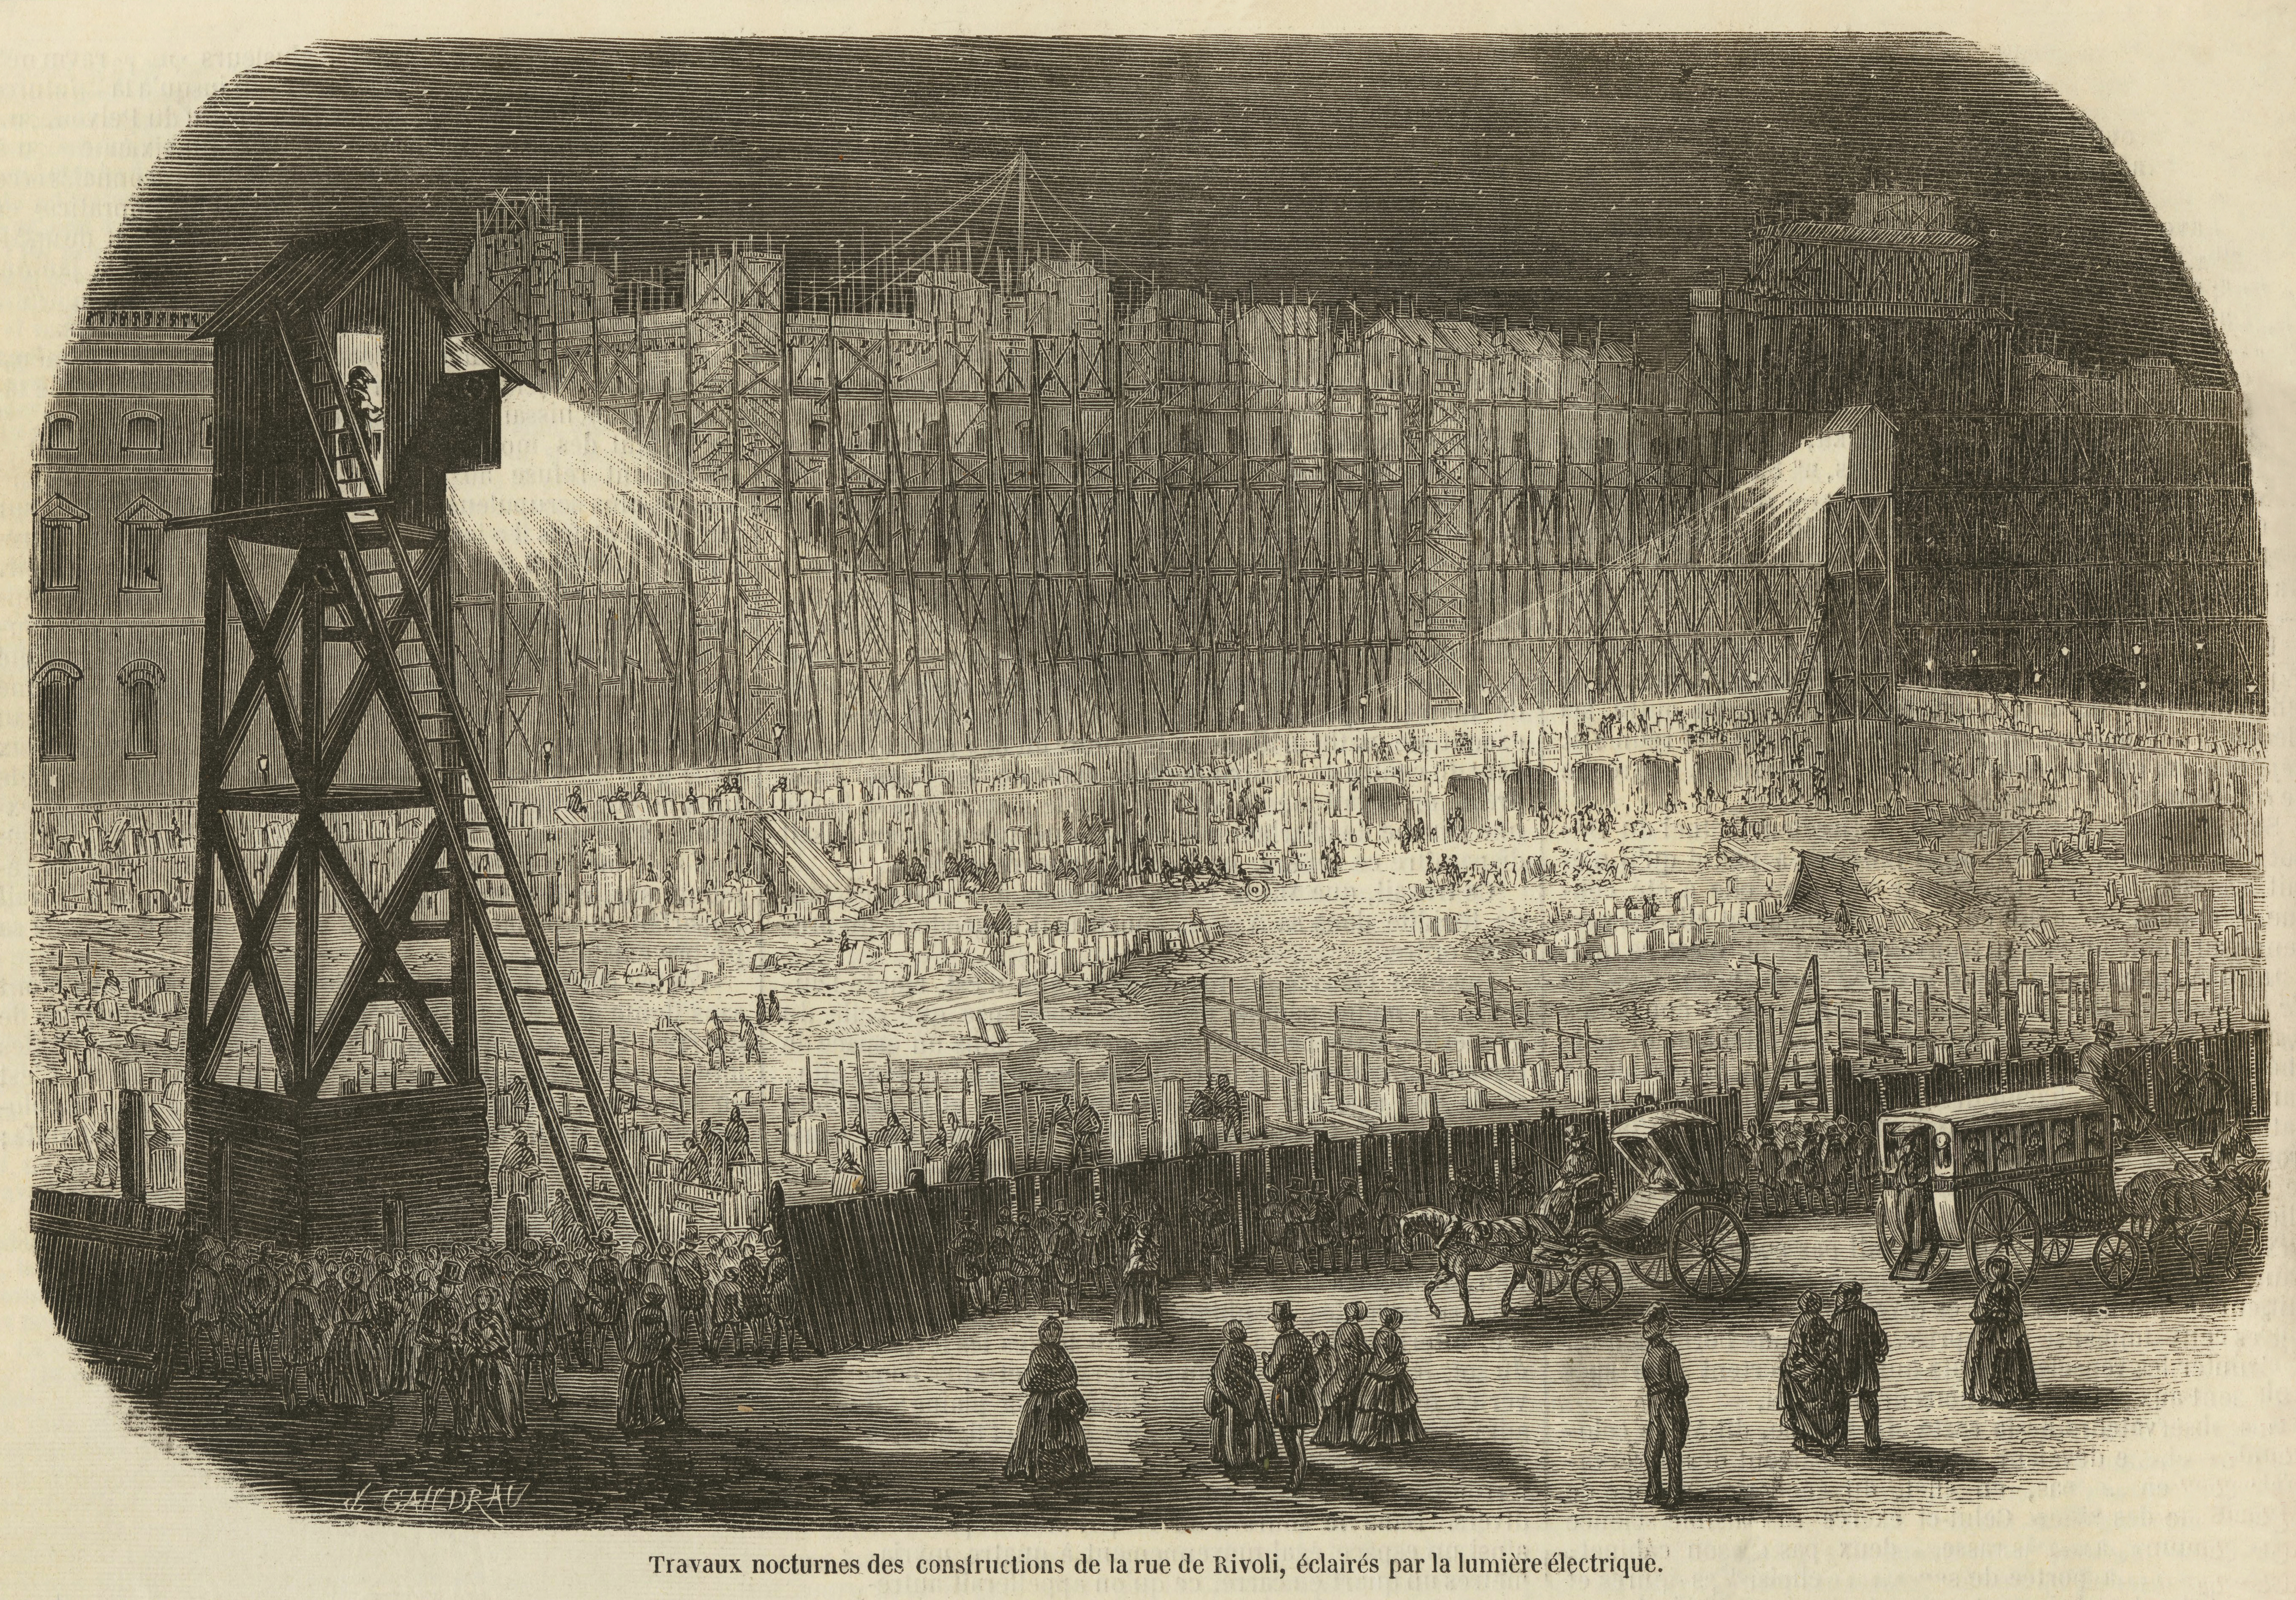
\includegraphics[width=1\textwidth]{2-cap1/complementos/fotos/rivoli.jpg}{\par \footnotesize Construção noturna da \textit{Rue de Rivoli}\textbf{Fonte:} \url{https://commons.wikimedia.org/wiki/File:Travaux_nocturnes_des_constructions_de_la_rue_de_Rivoli,_éclairés_par_la_lumière_électrique.jpg}. }
\label{fig:obrasrivoli}
\end{subfigure}
\end{figure}

A análise de exemplos poderia incluir a construção em Viena (Áustria) da \textit{Ringstrasse} e seus prédios monumentais por ordem do imperador Francisco José I (1857-1913) \cite{abercrombie_vienna_1910,abercrombie_vienna_1911,aman_vienna_1911}; poderia incluir o ``embelezamento'' de Bruxelas (Bélgica) sob a regência do burgomestre \textit{Jules Anspach} e do rei \textit{Leopoldo II} (\textit{le roi bâtisseur}, ``o rei construtor''), em especial o tamponamento e canalização do Sena entre 1859 e 1873 \cite{abercrombie_brussels1_1912,abercrombie_brussels2_1912,abercrombie_brussels3_1913}; poderia avançar pela expansão de Barcelona de acordo com o plano pioneiro de \textit{Ildefonso Cerdà} (1860) \cite{aibarbijker_barcelona_1997,ciervo_cerda_1976,soriaypuig_cerda_1995,wynn_barcelona_1979}; poderia seguir pelo \textit{Risanamento} de Florença (1865-1895), Nápoles (1885-1904) e outras cidades italianas em seguida à \textit{Unificazione} \cite{biocca_naples_1992,parisi_napoli_2001,piccinato_igiene_1989,rossi_napoli_2011}\dots Há um longo fio condutor a ligar o higienismo dos primeiro e segundo terços do século XIX ao ``proto-urbanismo'' do último terço deste mesmo século e ao urbanismo do primeiro terço do seguinte --- se é que há, realmente, alguma solução de continuidade, salvo pela escala e escopo das intervenções propostas nestes dois últimos casos. 

\begin{a3paisagem}
\begin{figure}[!htp]
\caption{Planta de situação da capital e da cidade residencial de Berlim e seus arredores --- plano de desenvolvimento dos arredores de Berlim (1856).}
\centering
\includegraphics[height=0.9\textheight]{2-cap1/complementos/mapas/1856_Bauplanungen.jpg}{\par \footnotesize \textbf{Fonte:} \url{https://commons.wikimedia.org/wiki/File:1856_Bauplanungen.jpg}.}
\label{fig:bauplannungen1856} 
\end{figure}
\end{a3paisagem}

\begin{a3paisagem}
\begin{figure}[!htp]
\caption{Plano para Berlim e arredores até Charlottenburg (1862), desenhado por Ferdinand Boehm.}
\centering
\includegraphics[height=0.9\textheight]{2-cap1/complementos/mapas/Boehm_Berlin_1862.jpg}{\par \footnotesize \textbf{Fonte:} \url{http://nbn-resolving.de/urn:nbn:de:kobv:109-opus-104224}. Os 14 departamentos do \textit{plano Hobrecht} estão rotulados como algarismos romanos. Os assentamentos programados estão indicados por letras maiúsculas e ruas por meio de algarismos arábicos, cada um dentro de um departamento de planejamento.}
\label{fig:berlin1862} 
\end{figure}
\end{a3paisagem}

\begin{a3paisagem}
\begin{figure}[!htp]
\caption{Plano de Giuseppe Poggi para Florença (1865).}
\centering
\includegraphics[height=0.9\textheight]{2-cap1/complementos/mapas/1865-planopoggi-florenca.jpg}{\par \footnotesize \textbf{Fonte:} \url{https://commons.wikimedia.org/wiki/File:Piano_Poggi_(Firenze,_1865)_-_1.JPG}.}
\label{fig:florenca1865} 
\end{figure}
\end{a3paisagem}

\begin{a3paisagem}
\begin{figure}[!htp]
\caption{Plano da cidade de Heilbronn, por Reinhardt Baumeister (1879).}
\centering
\includegraphics[height=0.9\textheight]{2-cap1/complementos/mapas/heilbronn.jpg}{\par \footnotesize \textbf{Fonte:} \url{https://commons.wikimedia.org/wiki/File:Stadtbauplan_Heilbronns_von_1879_auf_der_Grundlage_des_Generalbebauungsplanes_von_Reinhard_Baumeister.jpg}. }
\label{fig:heilbronn1879} 
\end{figure}
\end{a3paisagem}

Para os fins desta pesquisa, entretanto, os dois casos paradigmáticos apresentados já demonstram, sem necessidade de análise detalhada de outros exemplos, que o alvo preferencial das políticas do higienismo no século XIX foram os \textit{centros urbanos ditos ``degradados''} e as \textit{construções insalubres}. Ora, mas \textit{quem morava em tais construções e centros era exatamente quem não tinha condições de pagar para morar em imóveis em condições mais higiênicas}; ``higienizar'', ``embelezar'', fazer ``melhoramentos'' implicou, na maioria dos casos, em \textit{processos maciços de remoção dos trabalhadores e dos mais pobres dos bairros centrais}\footnote{No caso francês, \citeonline[p.~445]{faure_paris_2004} registra que ``dos 102 imóveis construidos nos anos 1860 pela companhia imobiliária dos irmãos Péreire, no atual bulevar Voltaire --- ou seja, num \textit{faubourg} do leste de Paris --- apenas 19\% dos apartamentos, dado o valor dos alugueis, parecem, a rigor, acessíveis a famílias operárias, a menos que se trate de cubículos nos sótãos''. Diz ainda que ``as operações de 1849-1853 tiveram como efeito desalojar 9.081 'trabalhadores' \([\dots]\): 2,1\% partiram para os \textit{banlieues}, e a imensa maioria dos outros se distribuiriam nos \textit{faubourgs}, uma reduzida minoria tendo permanecido nos bairros do centro, esperando, sem dúvida, que a continuação das obras não lhes desse caça'' (\Ibidem[p.~445]{faure_paris_2004}). No caso napolitano, tanto antes quanto depois do \textit{Risanamento} \citeonline{serao1906ventre} denunciou o caráter deletério das condições de vida dos trabalhadores mais pobres. No caso vienense, a \textit{Ringstrasse} acentuou a segregação socioespacial já existente, separando os burgueses da nova e resplandescente avenida, os operários dos subúrbios industriais como \textit{Ottakring} e uma pequena burguesia saudosa da antiga cidade \cite[p.~26]{maderthanermuser_vienna_2003}.}. O longo experimento higienista do século XIX interferiu também sobre a moradia, em especial sobre a moradia dos trabalhadores. A \textit{habitação operária} tornou-se, em paralelo à questão sanitária, pauta importante para os gestores públicos e os encontros internacionais de arquitetos e engenheiros: infiltou-se no Congresso Internacional de Higiene de 1878 em Paris \cite{congres_hygiene_1878}, fato repetido nos congressos internacionais de arquitetos de Londres (1908) e Viena (1910) \cite{QUINTOJR1990}, e mereceu um congresso internacional voltado apenas ao seu debate \cite{fleming_housing_1897}. Em nenhum deles, entretanto, chegou-se a qualquer solução definitiva quanto à questão, restringindo-se tais encontros ao relato das experiências locais em habitação operária e a soluções tópicas\footnote{Veja-se, como exemplo, o voto final da sessão plenária de 7 de agosto do Congresso Internacional de Higiene de 1878: depois de longos relatos e debates sobre a habitação dos operários em Paris, Londres, Bruxelas e outras metrópoles europeias, os presentes concordaram numa única recomendação: reforçar a legislação urbanística existente e transformar em exigência legal a instalação de água nas casas para operários \cite[p.~597]{congres_hygiene_1878}.}.

Tudo indica, até o momento, que os conflitos sociais são elemento essencial da produção, apropriação e uso dos territórios urbanos no período. Mas se há conflito social neste âmbito, seria a estética arquitetônica, ela própria, também produto dos conflitos sociais de seu tempo? Ou estaria imune a tal influência?

\subsubsection{As artes de morar: ecletismo e pré-modernismos, por dentro e por fora}\label{subsec:armor}

Entre os estilos arquitetônicos dezenovistas, o que mais interessa a esta pesquisa, pelo que se pôde encontrar nos documentos consultados, é o \textit{eclético}, do qual serão apresentados alguns exemplos --- retirados da magistral coletânea textbf{L’architecture privée au XIXe siècle, sous Napoléon III}, de César Denis Daly --- na \autoref{fig:hotelprimclas}, na \autoref{fig:hotelsegclas}, na \autoref{fig:villaprimclas}, na \autoref{fig:villasegclas1}, na \autoref{fig:villasegclas2} e na \autoref{fig:villaterclas}\footnote{Ao final da dissertação, nos \autoref{cap:anexos}, será possível encontrar plantas selecionadas de prédios residenciais e comerciais construídos entre 1889 e 1930 no distrito de Brotas, que poderão com proveito ser comparados com estes exemplos.}.

% resumidamente conceituado por um especialista como

% \begin{citacao}
% a cultura arquitetônica própria de uma classe burguesa que dava primazia ao conforto, amava o progresso (especialmente quando melhorava suas condições de vida), amava as novidades, mas rebaixava a produção artística e arquitetônica ao nível da moda e do gosto \cite[p.~13]{patetta_ecletismo_1987}.
% \end{citacao}

% A própria etimologia grega da palavra --- o adjetivo \textgreek{ἐκλεκτικός}, \textit{eklektikos}, ``escolhido entre os melhores'', por sua vez derivado de \textgreek{ἐκλεκτός}, \textit{eklektos}, ``escolhido, seleto'' --- indica uma de suas características principais: a escolha pelo arquiteto ou por seus clientes, na tradição arquitetônica passada, de elementos ora coerentes, ora díspares, que compusessem a obra de acordo com o gosto do freguês ou com a função a ser dada ao imóvel. Justo por isto, há enorme heterogeneidade estilística no campo eclético, sendo bastante difícil encontrar elementos comuns que não as justaposições e os revivalismos. 

% Como movimento artístico, o ecletismo ocorre na arquitetura e na arte do século XIX. As primeiras vanguardas desse movimento datam da terceira década do século XIX com a afirmação de pulsões neo-góticas em áreas francófonas e neo-renascentistas em Florença. Por volta de 1840, na França, em reação à hegemonia do estilo greco-romano, os arquitetos começam a propor a retomada de outros modelos históricos como, por exemplo, o gótico e o românico. O principal teórico do ecletismo arquitetônico é o francês \textit{César Denis Daly} (1811-1893) que o entende como ``o uso livre do passado''. Não se trata de uma atitude de simples copista, mas da habilidade de combinar as características superiores desses estilos em construções que satisfaçam a demandas da época por todo tipo de edificação. Na segunda metade do século XIX, o ecletismo tem forte presença na Europa. O estilo \textit{Segundo Império} ou \textit{Napoleão III} é caracterizado pela realização de importantes edifícios ecléticos, como o Teatro Ópera de Paris, projetado por \textit{Charles Garnier} (1825-1898).

\begin{figure}[!htp]
\centering
\caption{\textit{Hôtel privé} de primeira classe no estilo Segundo Império/Napoleão III.}
\includegraphics[width=1\textwidth]{2-cap1/complementos/fotos/daly01-0.JPEG}{\par \footnotesize \textbf{Fonte:} \textbf{L’architecture privée au XIXe siècle, sous Napoléon III:} nouvelles maisons de paris et des environs, de César Denis \citeonline{daly_architecture1_1864}. \par}
\label{fig:hotelprimclas} 
\end{figure}

\begin{figure}[!htp]
\centering
\caption{\textit{Hôtel privé} de segunda classe no estilo Segundo Império/Napoleão III.} 
\includegraphics[width=1\textwidth]{2-cap1/complementos/fotos/daly01-1.JPEG}{\par \footnotesize \textbf{Fonte:} \textbf{L’architecture privée au XIXe siècle, sous Napoléon III:} nouvelles maisons de paris et des environs, de César Denis \citeonline{daly_architecture3_1864}. \par}
\label{fig:hotelsegclas} 
\end{figure}

\begin{figure}[!htp]
\centering
\caption{\textit{Villa suburbaine} de primeira classe no estilo Segundo Império/Napoleão III.}
\includegraphics[width=1\textwidth]{2-cap1/complementos/fotos/daly03-4.JPEG}{\par \footnotesize \textbf{Fonte:} \textbf{L’architecture privée au XIXe siècle, sous Napoléon III:} nouvelles maisons de paris et des environs, de César Denis \citeonline{daly_architecture3_1864}. \par}
\label{fig:villaprimclas} 
\end{figure}

\begin{figure}[!htp]
\centering
\caption{\textit{Villas suburbaines} de segunda classe no estilo Segundo Império/Napoleão III.}
\begin{subfigure}[b]{0.8\linewidth}
\includegraphics[width=0.9\textwidth]{2-cap1/complementos/fotos/daly03-5.JPEG}
\caption{\textbf{Fonte:} L’architecture privée au XIXe siècle, sous Napoléon III: nouvelles maisons de paris et des environs, de César Denis \citeonline{daly_architecture3_1864}.}
\label{fig:villasegclas1}
\end{subfigure}
\
\begin{subfigure}[b]{0.8\linewidth}
\includegraphics[width=0.9\textwidth]{2-cap1/complementos/fotos/daly03-6.JPEG}
\caption{\textbf{Fonte:} \textbf{L’architecture privée au XIXe siècle, sous Napoléon III:} nouvelles maisons de paris et des environs, de César Denis \citeonline{daly_architecture3_1864}.}
\label{fig:villasegclas2}
\end{subfigure}
\end{figure}

\begin{figure}[!htp]
\centering
\caption{\textit{Villa suburbaine} de terceira classe no estilo Segundo Império/Napoleão III.}
\includegraphics[width=1\textwidth]{2-cap1/complementos/fotos/daly03-8.JPEG}{\par \footnotesize \textbf{Fonte:} \textbf{L’architecture privée au XIXe siècle, sous Napoléon III:} nouvelles maisons de paris et des environs, de César Denis \citeonline{daly_architecture3_1864}. \par}
\label{fig:villaterclas} 
\end{figure}

% As diferentes linguagens artísticas foram reelaboradas a critério do arquiteto seguindo a sua inspiração pessoal. No princípio a tendência eclética se impôs especialmente na realização de estruturas para festas e grandes eventos; sucessivamente, começou a ser apreciada também para mobiliar casas e jardins, nos quais, frequentemente e de forma totalmente acrítica, misturavam-se tempos gregos, vasos árabes e pavilhões indianos. Na época afirmou-se o costume de mobiliar cada sala das residências mais luxuosas segundo um estilo diferente. Assim, marceneiros e ebanistas, por exemplo, tiveram que aprender a lidar com formas bastante diferentes entre si. 

% Mas foi o modernismo industrial do século XIX que serviu como trampolim para o sucesso do estilo eclético. Em 1851, pela primeira vez, na \textit{Great Exhibition} em Londres foram realizados pavilhões onde os mercadores das principais nações do mundo foram chamados para expor suas próprias obras. Percebeu-se que as empresas presentes exibiam para a atenção do publico obras que mostravam a história recente ou antiga da própria nação. Houve euforia em expor todas as obras antigas remodeladas, havendo-se, inicialmente, um certo grau de dependência relativamente aos modelos originais, quase como se fosse uma cópia, uma reprodução. A fantasia de cada artista, artesão, arquiteto, ourives, etc. não demorou para se afirmar, levando os artistas a formular obras personalizadas que ``condensavam'' vários séculos de história. Era isso o que os clientes queriam, curiosos por artes distantes e citações culturais magníficas mostrando que aquela geração iria reviver uma era áurea. Todas as grande técnicas do passado reviviam numa miríade de moveis, cerâmicas e
objetos do Ecletismo.

% Grosso modo, as obras arquitetônicas em estilo eclético podem ser classificadas em três categorias principais, cujas características são assim definidas:

% \begin{itemize}
% \item A \textit{composição estilística}: caracteriza-se por um \textit{maior rigor filológico} e pela \textit{imitação precisa e coerente de um único e preciso estilo arquitetônico}. Os exemplos mais destacados são o \textit{neogrego}, o \textit{neo-egípcio} e o \textit{neogótico}.
% \item O \textit{historicismo tipológico}: caracteriza-se por uma \textit{relação apriorística de cunho analógico entre estilo e função} através de valores associativos, não raro arbitrários. A arquitetura medieval, por exemplo, forneceu aos arquitetos os traços místicos e a religiosidade para as novas igrejas; na arquitetura renascentista foram encontradas as características áulicas elegantes para os edifícios públicos; na arquitetura barroca, ou nos estilos orientais, a festividade exigida pelos equipamentos; no classicismo pesado do coríntio romano, o caráter apropriado aos solenes edificios parlamentares, aos museus e aos ministérios.
% \item Os \textit{pastiches compositivos}: caracterizam-se pela \textit{fusão de elementos arquitetônicos de estilos distintos, historicamente inadmissíveis}, sob cujos elementos díspares, não raro beirando o mau gosto, mascaravam-se muitas vezes soluções estruturais inovadoras \cite[p.~14-15]{patetta_ecletismo_1987}.
% \end{itemize}

A literatura especializada por muito tempo divergiu acerca do eclético. Primeiro considerou-o como o estilo ostentatório dos \textit{nouveaux riches} desprovidos da bagagem cultural do \textit{Ancièn Régime} e dispostos a demarcar seu espaço social por meio da sobreposição, às vezes sem nexo, das novas modas da Escola de Belas-Artes de Paris \cite[pp.~315-319]{guerrand_espacos_2009}. Num momento seguinte, considerou-o um estilo arquitetônico com méritos e conquistas próprios, em processo de redescoberta desde pelo menos a metade dos anos 1970, a partir da crítica ao ideário arquitetônico do Modernismo que o sucedeu e criticou duramente \cite{almeida_victoria_1997, almeida_vitrinescomercio_2014, patetta_ecletismo_1987, puppi_hisnamod_1998}. A discussão sobre a \textit{natureza estética} do eclético, ou de seus \textit{méritos técnicos e arquitetônicos}, é totalmente marginal a esta pesquisa. Interessa, sim, o fato de o eclético ser o estilo arquitetônico mais encontrado no distrito soteropolitano estudado.

%, especialmente nas modalidades de \textit{historicismo tipológico} e \textit{pastiche compositivo}, com maior frequência esta última.

A América Latina foi terreno fértil para as experimentações arquitetônicas, especialmente as ecléticas, e isto por questões muito particulares. No final do século XIX, findos os processos independentistas, consolidadas as fronteiras nacionais e assentados os blocos hegemônicos na política após um século pontilhado por guerras, \textit{pronunciamientos} e rebeliões, as classes dominantes nos países latinoamericanos viram na arquitetura um meio de reafirmar sua identidade nacional. Curiosa e paradoxalmente, entretanto, tal como em outros campos da cultura, esta reafirmação se deu por meio de símbolos e elementos tomados de empréstimo por estas mesmas classes dominantes às edificações da aristocracia, dos banqueiros, dos grandes comerciantes e industriais da Europa \cite[pp.~403-406]{gutierrez_arquibero_1983}. Conquanto haja leitura destes empréstimos no sentido de criar uma clivagem entre colonizados e colonizadores, em que os primeiros --- como um todo, sem qualquer clivagem, estruturação, estratificação ou hierarquização social internas a si próprios --- encontrar-se-iam sempre no encalço destes últimos por quaisquer razões \cite{bhabha_local_1998,memmi_coloniza_1967}, na perspectiva adotada por esta pesquisa parece mais plausível radicar estes empréstimos nos deslocamentos miméticos de ideias e práticas devido à \textit{inserção subordinada destas classes dominantes no capitalismo internacional e no colonialismo} \cite{schwarz_ideias_1973}. As duas correntes, entretanto, concordam em que o deslocamento de ideias, símbolos e signos de seu contexto original produz efeitos bastante diversos no novo contexto em que se inserem, e que são eles, e não aqueles produzidos em seu ambiente de origem, que devem ser estudados. Esta ``chave de leitura'' será importante para a análise da urbanização brasileira na Primeira República, mais adiante.

E aqui, nesta etapa ``pré-modernista'' do pensamento e da prática acerca das cidades, se encerram as condicionantes sincrônicas internacionais relevantes para a presente pesquisa. As defasagens entre a produção e circulação de ideias nos meios profissonaics levam a que as primeiras influências da arquitetura e do urbanismo europeus de vanguarda surgidas entre a última década do século XIX e as duas primeiras décadas do século XX, em seu pensamento ou realizações, só se façam sentir sobre o pensamento e a prática da arquitetura e do urbanismo em Salvador nos trabalhos da Semana de Urbanismo de 1935, que extrapolam o limite temporal escolhido\footnote{É certo, por exemplo, que Theodoro Sampaio mencionou explicitamente a influência sobre ele exercida pelas cidades-jardim \cite{costa1996theodoro}, e que já em 1913 estas mesmas cidades-jardins eram debatidas na imprensa baiana como contraponto ao desleixo da administração pública com o problema das moradias populares \cite{flexor_salvadorverde_2000}; apesar disto, nem o projeto da Cidade da Luz foi adiante (sua implementação em 1937 se deu vinte e oito anos depois da apresentação do projeto original de Theodoro Sampaio), nem os debates na imprensa avançaram além do confronto de ideias.}.
\section{A inserção brasileira no contexto internacional}\label{sec:insbrascontint}

É tempo, agora, de entender a inserção brasileira num contexto internacional de imperialismo, guerras, trustes e carteis. Nesta escala, já é possível analisar mais cerradamente a formação social e analisar, ainda que superficialmente, sua estrutura de classes, para, posteriormente, verificar a inserção da sociedade soteropolitana neste quadro.

\subsection{Da República da Espada (1889-1894) à República do Café-com-Leite (1894-1930)}\label{subsec:espadaleite}

A proclamação da república no Brasil (1889) resulta não apenas das questões \textit{religiosa}\footnote{Costuma-se dar este nome a uma série de conflitos ocorridos entre 1873 e 1876 entre o clero e a maçonaria, de um lado, e entre o clero e a instituição regalista do \textit{padroado}, de outro; ambos podem ser enquadrados na \textit{reação ultramontana católica} iniciada no papado de Gregório XVI (1831-1846) e continuada no papado de Pio IX (1846-1878), especialmente por meio da encílica \textit{Quanta Cura} e seu infame anexo \textit{Sílabo dos Erros} (1864) e das posturas mais duras do Concílio Vaticano I (1869-1870), como resposta às revoluções liberais e ao secularismo. O conflito do clero com a maçonaria já se antecipava enquanto ordem papal em \textit{Quanta Cura} e no \textit{Sílabo dos Erros}, ambos contrários à liberdade de consciência e ao primado da razão; restou que Vital de Oliveira, bispo de Olinda, e Macedo Costa, bispo do Pará, acendessem o pavio aplicando tais doutrinas a seu pastorado, proibindo maçons em irmandades católicas, punindo padres maçons e engajando-se em polêmica impressa contra a maçonaria. O caso chegou até à Coroa, pois o regalismo instituído pelo padroado facultava ao imperador brasileiro interferir em assuntos clericais -- na prática, a igreja era quase totalmente submissa à Coroa, fato condenado tanto em \textit{Quanta Cura} quanto no \textit{Sílabo dos Erros}. Com a subsequente prisão dos bispos por desobedecerem à ordem imperial de suspender as sanções religiosas que haviam imposto aos maçons, a questão tomou vulto, transformou-se em transtorno diplomático com o Vaticano, resolvido com a absolvição imperial dos bispos em 1876, passando assim a Pedro II a imagem de ``submisso ao Papa'' tão fortemente aproveitada pela campanha republicana então nascente.}, \textit{militar}\footnote{Entre 1884 e 1887, uma série de incidentes envolvendo o tenente-coronel Antonio de Sena Madureira e o coronel Ernesto Augusto da Cunha Matos em questões que iam desde protestos quanto à contribuição obrigatória para o montepio militar ou o afastamento de oficiais acusados de corrupção geraram intensa polêmica impressa, resultando na proibição, por parte do Ministério da Guerra, de qualquer manifestação de militares através da imprensa. A mordaça gerou insatisfação na caserna, especialmente na Escola Militar da Praia Vermelha, onde já floresciam a filosofia positivista e o republicanismo.} ou mesmo da questão \textit{sucessória}\footnote{Uma vez que Pedro II teve apenas filhas como herdeiras e a constituição brasileira de 1824 instituíra a sucessão semi-agnática, que não exclui herdeiras do processo sucessório, Isabel era a herdeira do trono brasileiro; por ser casada com Luís Filipe Maria Fernando Gastão, conde d'Eu, tido como largamente impopular em razão de sua nacionalidade francesa, sua futura ascensão ao trono criou entre as classes populares, a classe média, os militares e outros a má expectativa de serem governados por um estrangeiro.}; por importantes que sejam estas questões como expressão das contradições e conflitos sociais do último período do Império, foi fundamentalmente da crise aberta pela \index{abolição da escravidão}\textit{abolição da escravidão}, como corolário da degenerescência do regime escravista, que resultaram os problemas sociais e políticos que levaram à derrocada do Império. 

Foi, na verdade, nos anos 1860 que se acumularam fatores contrários à sustentação do regime escravista: a crise econômica dos anos 1860, causada pelo declínio nos preços do café (principal pauta de exportação brasileira na época); a crise financeira de 1864; a vitória dos Estados antiescravistas na Guerra de Secessão estadunidense, com o consequente debilitamento dos Estados escravocratas (Brasil e Cuba) perante a opinião pública internacional; a Guerra do Paraguai, onde massas de recém-libertos incorporadas à tropa são tomadas pelas ideias de liberdade e insuflaram-nas entre a oficialidade; o declínio da população escrava e as migrações internas de escravos, especialmente do Norte-Nordeste, para as regiões cafeeiras; tudo isto, enfim, resultou não apenas numa cúpula ministerial favorável à abolição, mas também ao florescimento de uma opinião pública também abolicionista, e ao surgimento das primeiras associações dedicadas à propaganda anti-escravista e à coleta de donativos para compra de alforrias \cite[p.~141-143]{gorender_escrareab_1990}.

É igualmente o momento em que não apenas a rebelião negra contra a escravidão, afogada pela maré montante da repressão no início do período, assume ao seu final novas formas e se intensifica; é de igual modo momento do dealbar, na cena política e social, de uma classe média urbana patrocinadora de um movimento abolicionista radicalizado, promotor não só da cotização para alforrias, mas igualmente de fugas individuais e coletivas de escravos \cite[p.~267-336]{saes_estadoburgues_1985}.

A \textit{abolição da escravidão} (1888) e a \textit{proclamação da república} (1889) fazem parte de um só processo de conflitos sociais no Império, em que as oligarquias agrárias enfrentaram não apenas os escravos rebeldes, mas igualmente uma classe média urbana estreante no cenário político; entendê-las separadamente implica numa separação injustificada entre entre uma esfera econômica e uma esfera política que só se podem compreender juntas. E muitas das contradições e conflitos sociais da Primeira República foram ensaiados já neste processo.

\subsubsection{A curta República da Espada (1889-1894)}\label{subsubsec:espada}

O período imediatamente posterior à proclamação da república no Brasil foi convulsionado por agitações políticas de todos os tipos. Em disputa, não somente projetos políticos, mas o poder, e, em última instância, mesmo o regime.

A crônica da época diz que o golpe militar responsável pela proclamação da república foi articulado por um grupo de jovens oficiais sem muita inserção entre a base da tropa e sem maior articulação com o oficialato superior, convocado à última hora para a ação \cite[p.~16]{cardoso_govmil_1977}; por frágil que fosse, esta articulação abriu um período de rearticulação das bases e das forças sociais hegemônicas do país. 

Durante a ditadura militar conhecida como \textit{República da Espada} DESENVOLVER RELACIONANDO CONTRADIÇÃO ENTRE CAFEICULTORES E MILITARES

O governo de Floriano Peixoto foi uma nota dissonante. Ele pensava em construir um governo estável, acima das disputas locais, estaduais e regionais, cooptando quadros nas escolas civis e militares. Teria tudo para ser ferrenho adversário dos oligarcas agrários, mas rapidamente surgiu uma aliança entre Floriano e o Partido Republicano Progressista (PRP), pois ambas as partes percebiam os riscos que corria a jovem república e viam-se como garantidores do novo regime: os oligarcas, por perceberem em Floriano a única possibilidade de garantir a sobrevivência do regime contra as forças centrífugas já então em pleno curso\footnote{EXPLICAR}; DESENVOLVER FAZENDO A PASSAGEM PARA CAMPOS SALES

Em defesa da república, surgem durante o governo Floriano Peixoto os ``jacobinos'' de 1893-1897, agrupados em torno de jornais como \textit{O Jacobino} e \textit{O Nacional}: gente como Júlio de Castilhos, Francisco Glicério, Deocleciano Martyr, Aníbal Mascarenhas e outros. Agitadores políticos profissionais, autoritários, anticlericais, defensores de medidas nacionalistas (tarifas de proteção à indústria e nacionalização do solo) e protetivas dos trabalhadores (como a jornada de oito horas e a regulamentação dos alugueis para operários), americanófilos e antilusitanos, atuavam ameaçando de morte os inimigos, intimidando-os com a publicação de seus nomes na sua imprensa (de longe a mais radical do período), provocando confrontos de rua, agitando o povo para depredações, insuflando ataques a portugueses (que tratavam, sem mais, como monarquistas) etc. \cite{queiroz_radicais_1986}\dots Tinham como base social principal o pequeno funcionalismo público e os militares de baixa e média patente. Com a perseguição aos suspeitos de envolvimento no atentado contra o presidente Prudente de Morais (5 nov. 1897), o movimento perdeu força e dissolveu-se.

Movimento monarquista (até declínio em 1910) \cite{CARONE1970inst,janotti_subversivos_1986} DESENVOLVER COMO A BAHIA FOI FOCO DO MOVIMENTO MONARQUISTA NO COMEÇO DA REPÚBLICA

\subsubsection{A longa República do Café-com-Leite, ou a Política dos Governadores (1894-1930)}\label{subsubsec:cafeleite}

DESENVOLVER EM SÍNTESE APERTADA, USANDO A Periodização de Edgar Carone: apogeu (Prudente de Moraes, Campos Sales, Rodrigues Alves, Afonso Pena), abalos (Hermes da Fonseca, Wenceslau Braz), contestações (Epitácio Pessoa, Artur Bernardes, Washington Luiz) \cite{carone_evolucao_1977}

DESENVOVER, EM SÍNTESE APERTADA A POLÍTICA DOS GOVERNADORES - funcionamento, altos e baixos 

DESENVOLVER O ARGUMENTO DE PERISSINOTO, NELSON WERNECK SODRÉ E BORIS FAUSTO; CONFLITOS REGIONAIS COMO CONFLITO ENTRE DIFERENTES FRAÇÕES REGIONAIS DOS LATIFUNDIÁRIOS, DIVIDIDOS ENTRE EXPORTADORES E PRODUTORES PARA O MERCADO INTERNO

\subsection{O Brasil, a banca internacional, o imperialismo}\label{subsec:brasimper}

A abolição e a proclamação da República criaram o quadro institucional adequado para a crescente integração do Brasil na economia capitalista mundial e colocaram o Brasil em posição de maior destaque na divisão internacional do trabalho, com um crescimento de 31,6\% nas exportações brasileiras entre 1880 e 1900 e de 63,7\% na primeira década do século XX \cite[p.~352]{singer_braecomu_1977}. 

Esta maior inserção, entretanto, se deu ainda no papel de fornecedor de matérias-primas e de produtos agrícolas, especialmente café (o principal produto da pauta de exportação brasileira), açúcar, algodão, borracha e derivados do couro.

\begin{table}[!htp]
\IBGEtab{
\caption{Brasil, principais produtos de exportação, 1889-1929 (em \%)}\label{tab:exportabrasil}}
{
\begin{minipage}{21cm}
\begin{tabular}{cccccccccc}
\hline
Períodos & Café & Açúcar & Cacau & Mate & Fumo & Algodão & Borracha & Couros/Peles & Outros \\
\hline\hline
1889-1897 & 67,8 & 6,5 & 1,1 & 1,2 & 1,7 & 2,9 & 11,8 & 2,4 & 4,8 \\
1898-1910 & 52,7 & 1,9 & 2,7 & 2,7 & 2,8 & 2,1 & 25,7 & 4,2 & 5,2 \\
1911-1913 & 61,7 & 0,3 & 2,3 & 3,1 & 1,9 & 2,1 & 20,0 & 4,2 & 4,4 \\
1914-1918 & 47,4 & 3,9 & 4,2 & 3,4 & 2,8 & 1,4 & 12,0 & 7,5 & 17,4 \\
1919-1923 & 58,8 & 4,7 & 3,3 & 2,4 & 2,6 & 3,4 & 3,0 & 5,3 & 16,5 \\
1924-1929 & 72,5 & 0,4 & 3,3 & 2,9 & 2,0 & 1,9 & 2,8 & 4,5 & 9,7 \\
\hline
\end{tabular} 
\end{minipage}
}
{ \fonte{Elaboração do autor, com dados de \citeonline[p.~63]{suzigan_polgov_2001}.} }
\end{table}

\begin{table}[!htp]
\centering
\IBGEtab{
\caption{Principais parceiros do Brasil no comércio internacional 1853-1928}\label{tab:comerbras}}
{\begin{tabular}{ccccccccc}
\hline
\multicolumn{9}{c}{Participação em \% no comércio exterior do Brasil} \\
\hline & \multicolumn{2}{c}{Grã-Bretanha} & \multicolumn{2}{c}{Alemanha} & \multicolumn{2}{c}{Estados Unidos} & \multicolumn{2}{c}{França} \\
\cline{2-9} Datas & Exp. & Imp. & Exp. & Imp. & Exp. & Imp. & Exp. & Imp. \\
\hline\hline
1853/4 a 1857/8 & 32,9 & 54,8 & 6,0 & 5,9 & 28,1 & 7,0 & 7,8 & 12,7 \\
1870/1 a 1872/4 & 39,4 & 53,4 & 5,9 & 6,5 & 28,8 & 5,4 & 7,5 & 12,2 \\
1902 a 1904 & 18,0 & 28,1 & 15,0 & 12,2 & 43,0 & 11,5 & 7,8 & 8,8 \\
1908 a 1912 & 17,0 & 27,5 & 14,3 & 16,2 & 38,2 & 13,5 & 8,6 & 9,4 \\
1920 & 8,2 & 21,4 & 5,8 & 4,6 & 42,0 & 40,6 & 12,0 & 5,4 \\
1928 & 3,4 & 21,0 & 11,0 & 12,3 & 44,6 & 26,2 & 9,0 & 6,2 \\
\hline
\end{tabular} }
{ \fonte{\citeonline[p.~369]{singer_braecomu_1977}} }
\end{table}

Para piorar, a fase monopolista do capitalismo, já detalhada na \autoref{sec:1.2}, implicava em enorme integração vertical e horizontal dos conglomerados empresariais, e igualmente de preferência pelos produtos destes conglomerados nas ``zonas de influência'' de seus países de origem; por isto, à exceção do café, para cuja produção o Brasil tinha características ecológicas excelentes, todos os demais produtos da pauta de exportação encontravam ou a concorrência de similares produzidos nas áreas de atuação dos conglomerados imperialistas (p. ex., açúcar de beterraba), ou o obstáculo de taxas aduaneiras protecionistas.

Percival Farquhar, conhecidíssimo capitalista estadunidense atuante no Brasil durante a República Velha \cite{CUNHA2011}, praticamente delineou, num artigo publicado em meio à guerra, o programa da ação dos investidores estrangeiros no país:

\begin{citacao}
Os notáveis investimentos na América do Sul serão, naturalmente, em estradas de ferro; serviços públicos urbanos; desenvolvimento da energia hidrelétrica; propriedades cujos produtos sejam consumidos nos Estados Unidos; títulos da dívida do governo federal, dos governos estaduais e dos municípios. \cite[p.~398]{farquhar_invest_1916}
\end{citacao}

Com algumas variações, este foi, na verdade o programa de atuação de todos os investidores estrangeiros no Brasil durante a Primeira República -- e o próprio Farquhar, por agir nas bancas de Londres, Paris e Bruxelas em busca de capital para seus empreendimentos, pode ser tomado como personagem-síntese desta atuação.

No que diz respeito aos empréstimos tomados pelo país junto à banca internacional, se apenas dois dos dos 17 empréstimos tomados pelo Brasil durante o Império se destinaram a investimentos em infraestrutura (estradas), após 1890 passam a se destinar majoritariamente a obras públicas (construção de portos e ferrovias) ou à sustentação das cotações externas de café. As dificuldades na quitação destas dívidas, comuns no Império, persistiram nas primeiras décadas da República: os dois \textit{funding loans} (1898 e 1914) foram pactuados pelo governo federal com a banca internacional mediante a cessão a exigências draconianas por esta última \cite[p.~365]{singer_braecomu_1977}.

\subsubsection{O capital britânico}\label{subsubsec:capbrit}

Os britânicos foram os principais beneficiados pela abertura dos portos brasileiros em 1808, e desde então dominaram o comércio externo e a banca brasileira.

A contração gradual começou por volta de 1928-1929 com a venda de diversos serviços públicos para corporações controladas por capitalistas estadunidenses, iniciando uma tendência sem retorno \cite{rippy_britlat_1954}.

DSENVOLVER USANDO A TABELA DE RIPPY

\subsubsection{O capital francês}\label{subsubsec:capfran}

Se os empresários franceses se faziam presentes no Brasil desde há muito, foi só durante a Primeira República brasileira que os investimentos franceses floresceram, como parte de uma tendência geral para investimento francês na América Latina (concentrado no Brasil, Argentina e México). Entre 1902 e 1914, os investimentos franceses na América Latina duplicaram, e os investimentos no Brasil passaram de 20\% a 42\% do total; além disso, em 1913 os investimentos diretos (ou seja, em empresas) ultrapassaram os empréstimos públicos, que até 1902 sempre haviam sido muito maiores em comparação \cite[p~83-84]{mauro_empfran_1999}. Entre 1904 e 1913 o Brasil foi o maior cliente da banca francesa na região, e o segundo em escala mundial \cite{rippy_french_1949}. 

Havia três destinos principais para os investimentos franceses: \textit{(a)} os \textit{portos}, em especial os de Recife, Porto Alegre e Rio de Janeiro; \textit{(b)} as \textit{ferrovias}, com especial destaque para a criação de seis companhias francesas específicas no setor e da  (1910), com capital de 3 milhões de francos, para a construção de ferrovias na Bahia; \textit{(c)} os \textit{bancos} \cite[p~84]{mauro_empfran_1999}, que merecem destaque.

O \textit{Banque Française au Brésil}, fundado em 1872 com capital de 10 milhões de francos, tornou-se lucrativo a partir de 1880, e mais ainda depois de 1900; o sistema financeiro francês, entretanto, ainda era insuficiente, o que levou à criação em 1909 do \textit{Banque Française et Italienne por l'Amérique du Sud} (conhecido posteriormente como \textit{Banco Sudameris}) \cite[p~84]{mauro_empfran_1999}. Entre um e outro, foram criados também o \textit{Banque Nationale du Brésil} (1893) e o \textit{Crédit Foncier du Brésil et de l'Amérique du Sud} (1907), este último tendo especial relevo nas muitas reformas urbanas realizadas no Brasil da Primeira República.

Os investimentos franceses no período gozaram de alta rentabilidade (taxas anuais de 5\%, com retorno rápido e prazos de amortização superiores a 35 anos), mas após a Primeira Guerra Mundial o franco se desvalorizou frente à libra esterlina, levando a uma conflituosa redução da dívida que só foi resolvida quando a Corte Internacional de Haia obrigou os devedores brasileiros a indexar a dívida segundo o franco-ouro \cite[p.~87]{mauro_empfran_1999}. Mesmo assim, em 1922 já havia 4 bilhões de francos investidos no Brasil\footnote{Distribuídos da seguinte maneira: 2,5 bi para empréstimos públicos, 1,25 bilhão para ferrovias, 170 milhões para bancos e 138 milhões para a indústria \cite[p~84]{mauro_empfran_1999}.}.

Até 1930, Pierre Louis Marcel Boilloux-Lafont era o mais importante capitalista francês a se relacionar com investidores e com o Estado brasileiro. Dono da \textit{Caisse Commerciale et Industriale} (fund. 1907), banco especializado em empréstimos estrangeiros, veio ao Brasil em 1909 para assumir a construção do porto de Salvador, e em 1911 conseguiu decreto autorizador do funcionamento da sua \textit{Societé Franco-Sud-américaine de Travaux Publics} no ramo da construção de estradas de ferro no Brasil; os 326 milhões de francos do grupo Boilloux-Lafont investidos no Brasil em 1914 representavam 10\% do total do investimento francês no país \cite{somogyi_lafont_1990}.

FALAR TAMBEM DO BARÃO FRANCÊS MUITO CITADO POR JOACI CUNHA

\subsubsection{O capital alemão}\label{subsubsec:capale}

As estatísticas divergem em alguns aspectos, mas é certo que a migração alemã para a América Latina não tomou vulto antes da década de 1850 \cite[p.~65]{rippy_german_1948} e só se tornou realmente significativa entre os anos 1880 e 1910 (cf. \autoref{tab:imigra}). Os primeiros migrantes foram responsáveis pelos primeiros empreendimentos comerciais de países latino-americanos com a Alemanha (antes mesmo da unificação) e por atrair investimentos alemães em terras, pecuária, imóveis, suprimentos agrícolas, cervejarias, hoteis e estabelecimentos mercantis. 

Havia na América Latina inteira em 1918 pelo menos 1.019 empresas com capital alemão, mobilizando US\$ 677 milhões \cite[p.~64-65]{rippy_german_1948}\footnote{As cifras estão em dólares, unusualmente para as estimativas do período, porque retiradas de \textit{blacklists} estadunidenses de empresas com participação alemã, usadas pelo governo dos EUA durante a Primeira Guerra Mundial como instrumento político para convencer governos latino-americanos a expulsar de seus respectivos países, ou ao menos de romper negócios e contratos pré-existentes.}. Ainda antes da Primeira Guerra Mundial, havia um pequeno circuito bancário alemão -- pequeno quando comparado com os circuitos britânico e francês -- constituído na América Latina: \textit{Banco Aleman Transatlantico}, \textit{Banco Germanico de la América del Sud}, \textit{Brasilianische Bank für Deutschland}, \textit{Banco de Chile y Alemania}, \textit{Banco Antioqueña}, \textit{Banco Mexicano de Comercio e Industria} e \textit{ZentralAmerika Bank}. Havia também outra especialidade alemã na América Latina, as empresas de navegação: Hamburg-American, Hamburg-South American, North German Lloyd, Hansa, Kosmos, Roland, Atlas e Kirsten Line \cite{rippy_german_1948}.

Não obstante sua presença marcante no campo da eletricidade e da química, reais especialidades da indústria alemã no período, em outros aspectos o capital alemão na América Latina era insignificante frente aos capitais britânico e francês. Antes da Primeira Guerra Mundial o capital alemão tinha pouca participação no setor de serviços públicos, somente duas petrolíferas, menos de doze mineradoras, quatro companhias de nitratos e três ferrovias (no valor total de US\$ 25 milhões), e participação tímida na indústia de processamento de carne, na navegação fluvial e na telefonia \cite{rippy_german_1948}. No Brasil, entretanto, sua presença foi marcante no setor agrícola.

MENCIONAR OS WILDBERGER COMO PARTE DO COMPLEXO GERMÂNICO; JUSTIFICAR A INCLUSÃO DE SUÍÇOS NESTA CATEGORIA

\subsubsection{Quadro geral}\label{subsubsec:quager}

ESCREVER TRANSIÇÃO AO CAPÍTULO

O Brasil já estava em recessão em 1928 \cite{hautcoeur_1929_2009} DESENVOLVER COM BASE NOS ARGUMENTOS DO AUTOR; POSIÇÃO POLÊMICA

A Bolsa do Café de Santos, um belíssimo prédio onde eram feitos pregões, registrava a tragédia em cifras: em agosto de 1929, dois meses antes da implosão da bolsa nova-iorquina, a saca do café estava cotada no mercado internacional em 200 mil-réis, em janeiro de 1930 desabara para 21 mil-réis. A praça de Santos, o maior centro brasileiro de atividades comerciais ficou virtualmente em moratória. Sem preços, o Brasil, que possuía 60\% do mercado internacional do café, não podia exportar o produto, e acumulava grandes estoques nos diversos armazéns gerais da cidade -- o que comprometeu os preços \cite{hautcoeur_1929_2009}.

CONTINUAR

\subsection{Classes sociais e política na Primeira República}\label{subsec:clapolprire}

Seria muito simples pegar a estrutura econômica brasileira e fazer derivar uma categoria profissional de cada um dos lugares na produção e, posteriormente, agrupá-los em classes mediante o critério da posse, propriedade ou controle dos meios de produção. 

Mas é isto suficiente?

Há vasta literatura recomendando prudência nesta caracterização \cite{aguiar_hierarquias_1974, BERNARDO1991, bernardo_fascismo_2015, ossowski_classes_1964, schumpeter_imperialismo_1961, velho_classes_1977}. Não há uma só entre as referências metodológicas consultadas que recomende tal simplismo empirista. É preciso, sim, entender como as classes se relacionam com seu lugar na produção econômica; entretanto, sem a força viva dos embates cotidianos e das pequenas coisas extra-laborais que fazem qualquer classe social fazer-se enquanto classe ao confrontar-se com outras (costumes, formas de sociabilidade, lazeres, produção cultural etc.), a análise terminaria manca.

Há ainda outra questão. É comum falar-se em ``elites'' para denominar qualquer estrato social dominante em determinado tempo e lugar. Tal classificação não será empregue nesta pesquisa, primeiro por ser vaga e imprecisa; segundo, por não respeitar a longa -- e controversa -- produção sociológica acerca do assunto \cite{bottomore_elites_1965,michels_partidos_1982,mosca_elementi_1923,pareto_mind_1935,
schumpeter_capitalismo_1961} terceiro, por só fazer sentido quando inserida num contexto teórico onde as classes sociais fornecem o substrato básico e as elites, um modo de compreensão da mobilidade social entre diferentes classes. Uma longa citação ajudará a situar o problema:

\begin{citacao}
\dots a referência a uma classe social só adquire sentido através da referência a uma classe oposta. A dialéctica da exploração e da opressão liga intimamente as características e a estrutura interna das várias classes, e sob este ponto de vista a luta entre as classes consiste na transformação conjunta e contraditória de todas elas. Mas não se passa o mesmo com a noção de elite, que pode ser definida de maneira independente, enquanto estrato privilegiado. A estrutura interna de uma elite nem se relaciona com a das massas, pois os teóricos das elites definem a massa precisamente pela sua incapacidade de organização própria, nem está em relação necessária com a estrutura interna de qualquer outra elite, porque a elite governa sozinha e se aparece uma nova é para liquidá-la e substituí-la. [\dots] a teoria das elites é incapaz de explicar, ou sequer conceber, esta transformação dos membros de uma elite em membros de uma classe. Os autores que pretendem que o fenómeno da mobilidade social invalida, ou pelo menos compromete, a teoria das classes e justifica a aplicação de uma perspectiva de elites estão a confundir classe com casta. É precisamente a mobilidade social que permite inserir o fenómeno das elites no quadro geral das classes, pois a formação de uma elite no interior de uma classe inferior prepara a projecção desta elite para a classe superior, alimentada periodicamente por estas novas elites [\dots]. As elites só têm sentido porque são elites de uma classe ou elites de uma classe transformando-se em componentes de outra classe. O conceito de elite padece, portanto, de uma assimetria, porque as elites capitalistas continuam a ser capitalistas, enquanto as elites proletárias abandonam a sua classe de origem. [\dots] a questão decisiva é que não ocorre nenhuma conversão de uma elite numa classe. Ou as elites se formam no interior de uma dada classe exploradora ou os membros da elite da classe explorada se convertem em membros de uma classe exploradora. \cite[p.~387-388]{bernardo_fascismo_2015}.
\end{citacao}

São igualmente inaplicáveis, para os fins desta pesquisa, os conceitos clássicos de \textit{oligarquia} e \textit{aristocracia}. Este último, porque com a proclamação da república foram extintos os títulos nobiliárquicos e todos os cargos políticos foram tornados eletivos pela Constituição de 1891; o primeiro, porque diz respeito a uma \textit{forma de governo} em que o exercício do poder político está restrito a um pequeno número de pessoas, não a uma \textit{classe social}, ou seja, aos fundamentos sociais do próprio poder político.

\subsubsection{Os latifundiários}\label{subsubsec:clagraris}

Dado o fato de a economia brasileira manter sua característica agroexportadora herdada do Império, são os \textit{latifundiários}, sem sombra de dúvida, uma das classes participantes do bloco político hegemônico durante a República Velha \cite{gorender_burguesia_1990,oliveira_emopro_1977,CARONE1970inst}. Há um debate em aberto acerca da natureza sociológica desta classe, em especial no período de transição do Império à República, girando em torno de ter-se ou não transformado numa \textit{burguesia agrária} por força da mudança de padrão da exploração do trabalho (da escravidão ao assalariamento) \cite{gorender_burguesia_1990,oliveira_emopro_1977}; para evitar as polêmicas, serão aqui chamados apenas de \textit{latifundiários} pelo fato de a raiz de seu poder político encontrar-se na exploração da produção agrícola em regime de \textit{plantagem}\footnote{Foi adotada aqui a denominação proposta por Jacob Gorender para o que tradicionalmente se chama \textit{plantation}. Eis a explicação, pelo próprio: ``As grandes explorações agrícolas com trabalho escravo, surgidas no continente americano à época do mercantilismo, têm sido designadas, na literatura de língua portuguesa, pelo nome de \textit{plantation}, vocábulo emprestado ao inglês e sempre impresso em itálico Mas os ingleses [\dots] tomaram o termo emprestado ao francês. [\dots] O esdrúxulo consiste em qu escritores de língua portuguesa precisem desse vocábulo estrangeiro a fim de indicar uma forma de organização econômica que Portugal teve muito antes da França e da Inglaterra (nas ilhas atlânticas) e que, no Brasil, apresentou-se sob um modelo clássico e de duração mais prolongada do que em outras regiões. Em lugar de \textit{plantation}, alguns autores empregam `plantação' ou `grande lavoura'. Ambas essas expressões linguísticas sofrem da desvantagem de carência de univocidade, prestando-se a confusões. Proponho substituir \textit{plantation}, em vernáculo, por plantagem. Não se trata aí de invenção léxica, porquanto plantagem está há muito dicionarizada. Mas, sendo vocábulo em desuso na linguagem comum e de todo ausente na literatura historiográfica e econômica, terá significação unívoca, além de dispensar o grifo e a pronúncia à inglesa \cite[pp.~119-120]{gorender_escracolo_2010}''.}. Esta classe social é quem se apropria do excedente produzido pela agricultura de exportação (café, açúcar, borracha, cacau etc.) e, por dominar a economia, reúne forças para dominar também a política e a sociedade.

Especialmente no Nordeste açucareiro, os impactos da abolição da escravidão foram drásticos: sendo os escravos bens de raiz que custavam, em conjunto, tanto ou mais que a própria terra que lavravam, sua libertação descapitalizou os donos dos velhos banguês, situação agravada pelo baixo preço internacional do açúcar, impeditivo da rápida recomposição do capital. Estas perdas, e também a baixa disponibilidade de capital excedente, levam os sucrocultores nordestinos a serem menos dispostos a arriscar em inovações tecnológicas -- exceto no caso pernambucano, onde a transição dos banguês para as usinas garantiu sobrevida econômica e política às frações inovadoras desta classe -- ou em mudanças de ramo de investimento \cite[p.~153]{CARONE1970inst}. 

No Sudeste, embora se possa falar de maior dinamismo, maior capital excedente e maior disponibilidade dos grandes cafeicultores para novos investimentos em tecnologia ou em outros ramos econômicos (como o comércio ou a indústria) \cite[p.~153-154]{CARONE1970inst}, não se pode esquecer que nem todos os cafeicultores seguiram este padrão, restrito a uma pequena fração da classe \cite[p.~32-38]{gorender_burguesia_1990}, e que a vasta maioria dos cafeicultores, por depender do mercado externo e suas flutuações, vivia endividada e sobre suas terras sobrepunham-se seguidas hipotecas \cite[p.~154]{CARONE1970inst}. 

Sua presença em todos os estratos governamentais significava, por isso, a garantia de políticas estatais de apoio financeiro à agricultura; o poder político é absolutamente dominado por esta classe durante toda a República Velha. No plano federal, todos os presidentes civis foram fazendeiros ou latifundiários; no plano dos Estados, a regra se repete \cite[p.~155]{CARONE1970inst}.

\subsubsection{A burguesia}\label{subsubsec:claburg}

Burguesia comercial DESENVOLVER, MOSTRANDO COMO OS COMERCIANTES SUBMETIAM OS LATIFUNDIÁRIOS POR MEIO DE CRÉDITO, DÍVIDAS E OLIGOPSÔNIO

Burguesia industrial DESENVOLVER, MOSTRANDO O CARÁTER SUBSIDIÁRIO FRENTE À PLANTAGEM

Os bons preços do café e a proibição de novas plantações, implementada em 1902, leva a camada mais dinâmica dos fazendeiros, como Rodrigues Alves, a aplicar capital próprio, retirado de suas lavouras, em comércio, bancos, indústrias e energia elétrica; o fenômeno se repetiu onde quer que boas safras ou inovações tecnológicas permitissem a formação de capital excedente, apto a ser reinvestido \cite[p.~147]{CARONE1970inst}

\subsubsection{Os trabalhadores}\label{subsubsec:clatrab}

Os trabalhadores são uma das classes globais do regime capitalista; conquanto esta afirmação tenha validade num plano lógico, teórico, num plano histórico, prático, sua formação assenta-se nos processos históricos de cada tempo e lugar. O que os põe juntos enquanto classe, num primeiro momento, é sua posição no processo de trabalho global, em oposição à dos burgueses e gestores; quaisquer outras ligações entre estes elementos da classe trabalhadora global dependem de sua ação nos campos político e cultural. É esta ação, assim como os processos históricos de sua formação enquanto classe, que precisam ser compreendidos em cada caso.

No caso brasileiro, houve uma coincidência de dois fatores: a chegada de uma massa de migrantes (italianos, espanhóis, portugueses, japoneses, alemães, poloneses, austríacos, lituanos, iugoslavos, húngaros, tchecos, romenos, russos etc.) para as cidades e campos, especialmente do Sul e Sudeste, de \textit{migrantes europeus} para servir como trabalhadores de baixa ou média qualificação, muitos dos quais -- não todos -- trazendo de seus países de origem ideologias e tradições próprias de organização, como o anarquismo e o socialismo \cite{petrone_imigra_1977}; e o longo processo de \textit{luta contra a escravidão}, no qual negros escravizados criaram formas próprias de negociação e resistência.

Não obstante ser possível entender que entre migrantes recém-chegados e negros recém-libertos do cativeiro houvesse sérios estranhamentos (especialmente por causa do racismo anti-negro); que correntes intelectuais como o socialismo e o anarquismo em cidades de menor porte permanecessem restritas a pequenos círculos intelectuais \cite{duarte_rebelde_1991}; que tais correntes tivessem problemas em adaptar-se a práticas e costumes locais, especialmente aos de origem africana \cite{goes_formacao_1988}; não obstante tudo isso, é certo que desde os primeiros anos da República, quando os migrantes ultrapassavam o racismo anti-negro em prol de questões comuns, estes dois setores envolveram-se em lutas conjuntas, e que os poucos trabalhadores manuais interessados na chamada ``questão social'' discutiam-na abertamente com seus companheiros de labor \cite[p.~73-85]{gomes_velhos_1988}; que formaram um potente movimento operário, simultaneamente reivindicativo e revolucionário \cite{samis_anabras_2004}, capaz de organizar as forças do trabalho nos planos político e cultural \cite{farinha_federa_2002,hardman_patripatr_2002}, de paralisar todo o trabalho de uma cidade por meio de greves gerais \cite{castellucci_salvador_2001,magnani_anarsp_1982} e inclusive de promover atos insurrecionais \cite{dulles_anacombras_1977,koval_prolbras_1982}. 

Este movimento, entretanto, circunscreveu-se aos trabalhadores \textit{urbanos}; os \textit{trabalhadores rurais}, em suas diversas formas históricas (parceiros, meeiros, moradores, arrendatários, safreiros, foreiros, boias-frias, agregados, colonos etc.) pouco se integraram a estas lutas no período estudado, embora movimentos como os de \textit{Canudos}, do \textit{Contestado} e a \textit{Revolta do Capim} (Pará) sejam de extrema relevância em seus respectivos contextos \cite{mottazarth_rescamp1_2008}. 

No que diz respeito à \textit{composição técnica} desta classe, as fontes censitárias de 1872 e 1920 refletem a divisão social do trabalho existente no país ao classificar como ``industriais'' profissões tão díspares quanto as ``artes e ofícios'' (marceneiros, ferreiros, mecânicos etc.), os trabalhadores artesanais e as indústrias caseiras \cite[p.~141]{pinheiro_prolind_1977}. Os trabalhadores ditos qualificados, os da construção civil e os dos transportes (terrestres e marítimos) conseguiam razoável grau de organização, mas os trabalhadores fabris eram, em sua maioria, mulheres e crianças, eram mais difíceis de organizar \cite[p.~152]{pinheiro_prolind_1977}. É possível dizer que, dada a pequena relevância da produção fabril na vasta maioria do território brasileiro, estes trabalhadores artesanais constituíssem a maioria da classe trabalhadora no período.

É de se indagar, no caso brasileiro, se chegou a se formar nestes movimentos a \textit{aristocracia operária} vituperada num só coro por anarquistas, socialistas e comunistas \cite{bakunin_contramarx_2015,engels_1892pref_1990,lenin_imperialismo_1987}. Os estudos realizados até o momento indicam a formação de uma \textit{camada superior} entre os trabalhadores urbanos, em geral formada por aqueles ligados às profissões artesanais (sapateiros, alfaiates, vidreiros, estucadores, marmoristas, calceteiros etc.) ou ligadas de algum modo à cultura (gráficos, professores etc.); e entre eles, formou-se uma camada ainda mais coesa o grupo daqueles que, por saber ler e escrever -- não se pode esquecer que no Brasil da época a taxa de analfabetismo variou entre 83\% (1890) a 65\% (1920) -- capitanearam as incontáveis iniciativas culturais operárias do período (escolas, grupos de teatro, círculos literários etc.) \cite{gomes_velhos_1988,goes_formacao_1988,hardman_patripatr_2002,pinheiro_prolind_1977}. Há, inclusive, quem classifique esta camada superior da classe trabalhadora já como ``classe média'' -- problema a ser discutido na \autoref{subsubsec:clamed}.

É importante observar, por outro lado, que esta camada estava apta apenas a exercer hegemonia \textit{cultural} sobre a classe, que não coincidia com a hegemonia \textit{política}. Os sindicatos do período, instrumento político por excelência dos trabalhadores num momento em que a proibição do voto aos analfabetos impedia-os de participar da política eleitoral mesmo no papel passivo de eleitores, eram organizados por ofícios (ou seja, para cada profissão um sindicato), e não por ramo industrial (ou seja, para cada cadeia produtiva um sindicato); isto garantia que mesmo os trabalhadores menos privilegiados podiam liderar suas categorias, e assim participar da ação política em pé de igualdade com as categorias profissionais mais elitizadas. As reivindicações trabalhistas eram tratadas no período pelos empresários com supremo desdém, quando não com violência; isto, e a criminalização das greves no Código Penal de 1890 (arts. 204 a 206), gerou a reação de ações igualmente violentas por parte dos trabalhadores, transformando cada greve numa potencial insurreição. Adicionalmente, embora a ação sindical existisse no Brasil desde a alvorada da república (ou mesmo antes dela \cite[p.~69-77]{koval_prolbras_1982}), o reconhecimento dos sindicatos como interlocutores pelos empresários via de regra era nulo, e os acordos ao final de cada greve eram feitos diretamente entre os patrões e os trabalhadores \cite{dulles_anacombras_1977,koval_prolbras_1982}. Soma-se a isso o fato de os poucos partidos denominados ``operários'' ou ``socialistas'' no período, além de absolutamente inexpressivos em termos eleitorais, serem em geral dominados pelas chamadas ``classes médias'' \cite[p.~150]{pinheiro_prolind_1977}, gerando um estranhamento impeditivo de sua transformação em reais instrumentos políticos dos trabalhadores. Para piorar, fora dos períodos de greve os sindicatos não conseguiam a mesma audiência dos períodos paredistas \cite[p.~152]{pinheiro_prolind_1977}. Sendo assim, esta camada superior, por privilegiada que fosse no seio da própria classe, não dispunha das condições para o mesmo tipo de ``aburguesamento'' verificado nas aristocracias operárias europeias. Esta aristocracia, conhecida no Brasil pelo nome de ``pelego'', só veio a ser formada quando da reestruturação corporativista do Estado brasileiro em 1937, quando os sindicatos foram transformados em órgãos estatais.

\subsubsection{O enigma da ``classe média'' urbana}\label{subsubsec:clamed}

Sociólogos, economistas e historiadores criticam o uso do termo ``classe média'' por ser vago, incerto e não ter ``base conceitual de origem controlada'' \cite[p.~19]{POCHMANN2014};  mesmo as ilustrações históricas do papel desta classe seriam ``insatisfatórias'' \cite[p.~9]{pinheiro_clamed_1977}. Há, inclusive, quem prefira, prudentemente, passar reta e silenciosamente por qualquer esforço conceitual, confiando no puro empirismo para analisar a ação política desta ``classe''. O máximo que se tentou fazer quanto a esta ``classe'' no período estudado foi subdividi-la em dois grandes grupos: a classe média \textit{antiga}, composta pelos pequenos produtores e pequenos comerciantes, e a classe média \textit{nova} \cite[p.~11]{pinheiro_clamed_1977}. Ou, ainda, dividi-la numa camada \textit{alta}, oriunda de setores da classe latifundiária por meio do bacharelismo; numa camada \textit{média}, composta por imigrantes, segmentos das classes decadentes, profissionais liberais, exército etc.; e numa camada \textit{baixa}, composta por artesãos e funcionários públicos \cite[p. ~175-176]{CARONE1970inst}. Foi tentado, também, diferenciar esta ``classe média'' segundo as características de sua inserção na estratificação social segundo o desenvolvimento histórico em cada região do país: se no Sul esta classe é formada por ``pequenos fazendeiros que abandonavam o campo, assim como colonos e seus descendentes que pretendiam subir na escala social'', no Norte ``as grandes famílias proprietárias decadentes forneciam contingentes de funcionários públicos, grupos profissionais, empregados de indústria e comércio, proprietários de pequenos negócios''  \cite[p.~16]{pinheiro_clamed_1977}.

A profusão de estratificações da ``classe média'', tal como as reiteradas confissões sobre as dificuldades de separá-las da classe trabalhadora ou de setores da classe latifundiária, testemunham o caráter problemático da categorização homogênea de tantos elementos heteróclitos. A ``classe média'' é tratada como classe distinta das demais por \textit{hábito}, mais que por construção conceitual precisa; entretanto, como quer que seja categorizada (e por maiores os problemas encontrados na sua conceituação), há vasta produção historiográfica sobre a atuação desta ``classe'' durante a República Velha, indicando não apenas a atuação de grupos sociais específicos, como também a pertinência do conceito, conquanto equívoco, para agrupá-los numa só ``classe''. Esta produção permitirá elucidar o enigma de sua caracterização sociológica -- o que, como se verá, só permite chamar a ``classe média'' de ``classe'' com muita insistência nas aspas.

Indo aos fatos, percebe-se que a República Velha reuniu as condições ideais para o florescimento desta ``classe''. Um primeiro exemplo é a proliferação das \textit{faculdades}, os criadouros de bacharéis, futuros burocratas. Em 1916 já havia 16 faculdades de Direito, que formavam cerca de 408 bacharéis por ano; não se pode esquecer que, na falta de cursos formais de Administração, Sociologia ou Economia, eram os bacharéis em Direito quem cumpria com suas atribuições, e muitos dos cursos jurídicos então existentes nomeavam-se de ``Ciências Jurídicas e Sociais''. Em 1920 foi criada a Universidade do Rio de Janeiro, atual universidade federal, primeira do país; em 1930, havia 350 estabelecimentos de ensino secundário e 200 de ensino superior \cite[p.~17]{pinheiro_clamed_1977}.

As grandes cidades reuniam num só espaço as repartições públicas e os cursos superiores; eram, desde a Colônia, o lugar por excelência de exercício das \textit{profissões artesanais} \cite{REIS2012}, e agrupavam também os negros recém-libertos, que a elas acorriam em massa para fugir -- temporária ou definitivamente -- da escravidão. O Rio de Janeiro era o lugar por excelência das ``classes médias'', por ser o maior entreposto comercial do país (com o consequente surgimento de postos de trabalho nos escritórios comerciais) e por ser a capital federal (com o consequente agrupamento espacial da burocracia correspondente) \cite[p.~119]{pinheiro_clamed_1977}, mas a emergência da burocracia estatal ou privada é fenômeno verificável em todas as capitais estaduais ou em cidades com função comercial destacada.

No que diz respeito à sua atuação política, o aparente antagonismo entre a ``classe média'' e os latifundiários era superficial, não correspondia a um antagonismo econômico; a ``classe média'' era economicamente dependente dos latifundiários, na medida em que durante toda a Primeira República brasileira desenvolveu-se o chamado ``estado cartorial'', uma política de angariamento de apoio político em troca de cargos na máquina pública \cite[p.~20]{pinheiro_clamed_1977}.

Comércio DESENVOLVER, FALANDO DOS PEQUENOS COMERCIANTES

 DESENVOLVER, FALANDO DOS CARGOS PÚBLICOS, DA PRESENÇA MAJORITÁRIA NO TERCIÁRIO ETC.

Concretamente, sua atuação foi tão oscilante quanto sua própria situação de classe. O florianismo e sua vertente radical, o jacobinismo, por exemplo, desenvolveram-se entre a ``classe média'' das grandes cidades brasileiras \cite{queiroz_radicais_1986}, mas já em 1910 esta mesma ``classe média'' apoiaria decididamente a campanha civilista de Rui Barbosa. Se no primeiro caso houve a aparência de autonomia de classe, isto se dá pela inserção -- certamente equivocada, como se verá na \autoref{subsubsec:milclaest} -- dos militares como elementos desta ``classe''; no segundo caso, a submissão da ``classe média'' às táticas políticas dos latifundiários é total, vez que a campanha civilista encontrou sua principal base entre latifundiários paulistas \cite[p.~28-29]{pinheiro_clamed_1977}.

Em suma: crescente em termos demográficos, por força da crescente complexificação da divisão social do trabalho no país, a ``classe média urbana'' aparentemente não teve durante a República Velha um desempenho político que visasse o aumento de seu poder no sistema político vigente, nem tampouco pautou questões voltadas à transformação radical do regime vigente \cite[p.~36]{pinheiro_clamed_1977}.

\subsubsection{Militares: classe ou estamento?}\label{subsubsec:milclaest}

DESENVOLVER O TEMA USANDO O ESTAMENTO WEBERIANO E A LEITURA DE HELOÍSA FERNANDES SOBRE O LUGAR SOCIAL DOS MILITARES

RESSALTAR QUE OS MILITARES TIVERAM POUCA RELEVÃNCIA POLÍTICA NA BAHIA, E QUE SE ORGANIZARAM PARA RESISTIR AO ``GOLPE'' REPUBLICANO NOS PRIMEIROS MOMENTOS

\subsection{As cidades brasileiras: reformas urbanas e regime de terras em tempo de monopólios}\label{subsec:cidbraref}

Tendo chegado à escala nacional, já é possível falar, malgrado as inevitáveis particularidades, de um \textit{contexto urbano} um pouco mais homogêneo.

Censitariamente, e mesmo com os cuidados a serem tomados no uso dos dados censitários anteriores a 1940\footnote{\citeonline[p.~24]{santos_urbanizacao_2005} observa que ``somente após 1940 as contagens separavam a população urbana (cidades e vilas) da população rural do mesmo município''.}, a evolução da urbanização brasileira, conquanto ``pequena e frágil'' \cite[p.~303]{suzigan_polgov_2001} e longe de alcançar os patamares do período iniciado na década de 1940, começava a se destacar (cf. \autoref{tab:popurbra}).

\begin{table}[!htp]
\centering
\IBGEtab{
\caption{Grau de urbanização do Brasil (1872-1920)}\label{tab:popurbra}
}{
\begin{minipage}{18cm}
\begin{tabular}{m{1cm} m{1.8cm} m{0.4cm} m{1.5cm} m{0.4cm} m{1.5cm} m{0.4cm} m{1.5cm} m{1cm} m{1cm} m{1cm}}
\hline 
\multirow{2}{*}{Censo} & \multirow{2}{*}{Pop. total} & \multicolumn{2}{c}{50 mil ou +} & \multicolumn{2}{c}{100 mil ou +} & \multicolumn{2}{c}{500 mil ou +} & \multicolumn{3}{c}{Pop. urbana (\%)} \\ 
\cline{3-11} & & nº & pop. & nº & pop. & nº & pop. & 50 mil ou + & 100 mil ou + & 500 mil ou + \\ 
\hline\hline
1872 & 9.930.478 & 4 & 582.749 & 3 & 520.752 & -- & -- & 5,9 & 5,6 & -- \\ 
1890 & 14.333.915 & 6 & 976.038 & 3 & 808.619 & -- & -- & 6,8 & 5,6 & -- \\ 
1900 & 17.438.434 & 8 & 1.644.149 & 4 & 1.370.182 & -- & -- & 9,4 & 7,9 & -- \\ 
1920 & 30.635.605 & 15 & 3.287.448 & 6 & 2.674.836 & 1 & 1.157.873 & 10,7 & 8,7 & 3,8 \\ 
\hline 
\end{tabular} 
\end{minipage}
}
{\fonte{Artigo ``Dos governos militares a Prudente – Campos Sales'', de F. H. \citeonline{cardoso_govmil_1977}}.}
\end{table}


Durante a República Velha, as cidades se desenvolveram dentro da dinâmica do sistema agrário-exportador; a urbanização se deu ``à sombra do fortalecimento da economia agrário-exportadora, que a longo prazo conformará o Estado à sua própria imagem, portanto, à própria burocracia''  \cite[p.~22-23]{pinheiro_clamed_1977}.

DESENVOLVER, FALANDO DO DESENVOLVIMENTO DAS GRANDES CIDADES TENDO AS CAPITAIS COMO EXEMPLOS

O \textit{higienismo}, como alhures, era a ideologia animadora dos debates em torno da situação das cidades; medicina e engenharia sobrepunham-se na definição do que era mais salubre para as cidades, propondo invariavelmente ambientes capazes de deixar sair os ``maus odores'' \cite{CAPONI2002}. Engenheiros sanitaristas como Saturnino de Brito, Lourenço Baeta Neves, Miguel Presgrave, Teodoro Sampaio, Bernardino de Queiroga, Victor da Silva Freire, Manoel Pereira Reis, Américo Rangel e José Pereira Rebouças desenvolveram planos urbanos (alguns chamados de ``planos de melhoramentos'' \cite{leme_urbasp_1991}) e coordenaram a execução de obras de saneamento; se não se diziam ``modernos'', suas concepções eram profundamente modernas \cite{andrade_saturnino_1991}. Entre os vários ``planos de melhoramentos'' da época, o mais conhecido é o realizado, em 1927, por convite do prefeito do Rio de Janeiro, Antonio Prado Junior, ao urbanista francês Alfred Agache: resultou daí um plano de extensão, embelezamento e remodelação para o Rio de Janeiro, apresentado em 1930 \cite{pinheiro_capiconsul_2009}.
\section{A sociedade baiana e soteropolitana num mundo em convulsão}\label{sec:sobasotconv}

É só depois de empreender este longo percurso que é possível entender a situação das sociedades baiana e soteropolitana no período. Estabelecidas as linhas gerais da economia, da política e da cultura, a narrativa do \textit{desajuste} da economia baiana frente aos núcleos mais dinâmicos do capitalismo, assim como a permanência atávica de certos traços culturais e políticos, pode ser compreendida sem maiores problemas.

Será preciso, para isto, compreender a inserção da Bahia na evolução nacional nos aspectos econômico, demográfico, social e cultural e a posição de Salvador neste processo; as razões da estagnação econômica do Estado e da paralisia demográfica de Salvador nas primeiras décadas do século XX; a formação de uma estratificação e de uma estrutura de classes sociais correspondente a uma economia baseada no trabalho livre, em substituição a uma estratificação e a uma estrutura de classes sociais correspondente a uma economia baseada no trabalho escravo; os lazeres públicos e as festas cívicas, laicas e religiosas, momentos onde expressavam-se de forma bastante ritualizada as distinções comportamentais e estéticas entre classes sociais.

\subsection{Demografia}\label{subsec:demogbasa}

A análise da população soteropolitana será feita com base nos censos de 1872, 1890, 1900, 1920 e 1940. O primeiro e o último serão incluídos, apesar de ultrapassarem o lapso temporal escolhido para esta dissertação, pelo fato de os censos programados para os anos de 1880 e 1930 não terem sido realizados por força de dificuldades políticas conjunturais \cite{oliveirasimoes_censos_2005}; da mesma forma, a precária apresentação dos censos de 1890 e 1900 mediante simples sinopse, sem qualquer tabela de detalhamento, levou a considerá-los nesta pesquisa apenas para simples contagem populacional municipal, sem qualquer outro item que se lhes aproveite \cite{reisetal_areascensos_2011}. 

Viu-se no século XIX a população soteropolitana mais que triplicar entre 1800 (50 mil hab.) e 1890 (174 mil hab.) \cite[p.~70]{sampaio_formas_1999}; é com base no puro impacto da triplicação que se costuma afirmar a existência de um forte crescimento demográfico no período. Ora, sem entrar na discussão das causas das variações populacionais sazonais, já bastante comentadas na historiografia -- cólera (1855, 1866), febre amarela (1849-1854), peste bubônica (1855), secas prolongadas no interior baiano (1857-1861, 1869-1870, 1877-1879, 1888-1890) etc. --, trata-se do acréscimo médio de aproximadamente 1.378 habitantes ao ano, e de uma taxa de crescimento populacional de 1,4\% ao ano (a.a.)\footnote{A taxa de crescimento populacional é calculada usando a metodologia do IBGE: \[ r = \Bigg[ \Bigg( \sqrt[n]{\frac{P_{0}}{P_{t}}} \Bigg) - 1 \Bigg] X 100 \] onde \textit{r} é a taxa de crescimento anual, \textit{$P_{0}$} é a população ao início do perído, \textit{$P_{t}$} é a população ao final do período e \textit{n} é o número de anos do período.}. Uma comparação com o crescimento populacional em outros períodos ajuda a situar a questão (cf. \autoref{tab:1}, p. \pageref{tab:1}).

\begin{table}[!htp]
\centering
\IBGEtab{
\caption{Evolução populacional de Salvador 1872-1940}\label{tab:1}}
{\begin{tabular}{|c|c|c|c|}
\hline 
Ano & População (hab.) & Variação (hab.) & Taxa média de crescimento (em \% a.a.) \\ 
\hline 
1872 & 129.109 & -- & -- \\ 
1890 & 174.412 & 45.303 & 1,68 \\ 
1900 & 205.813 & 58.401 & 1,67 \\ 
1920 & 283.422 & 77.609 & 1,61 \\ 
1940 & 290.443 & 7.021 & 0,12 \\ 
\hline 
\end{tabular} }{
\fonte{Elaboração do autor, com base nos Recenseamentos de 1872, 1890, 1900, 1920 e 1940.}}
\end{table}

Por esta perspectiva, apenas a taxa de crescimento verificada entre 1920 e 1940 pode ser considerada como ``ponto fora da curva'' por força das epidemias de gripe espanhola (1918), varíola (1919) e febre amarela (1919), causadoras de óbitos e de emigração; exceto por este período, a velocidade do crescimento demográfico soteropolitano manteve-se durante toda a Primeira República consistente com o verificado no século anterior, sendo mesmo ligeiramente maior.

Vista a questão em termos comparativos com outras cidades brasileiras, entretanto, aparece uma enorme defasagem entre este incremento demográfico e os do Rio de Janeiro e São Paulo, únicas cidades brasileiras demograficamente comparáveis a Salvador no período.

\begin{table}[!htp]
\centering
\IBGEtab{
\caption{Incremento demográfico segundo recenseamentos oficiais}\label{tab:2}}
{\begin{tabular}{|c|c|c|c|c|c|c|c|c|}
\cline{1-9}
\multirow{3}{*}{Capitais} &\multicolumn{8}{c|}{Aumentos populacionais}\\
\cline{2-9} & \multicolumn{2}{|c|}{1872-1890} & \multicolumn{2}{|c|}{1890-1900} & \multicolumn{2}{|c|}{1900-1920} & \multicolumn{2}{|c|}{1920-1940}	\\
\cline{2-9} &nº &\% &nº &\% &nº &\% &nº &\%\\
\cline{1-9} São Paulo &33.549 &106,89 &147.886 &269,32 &339.183 &141,43 &747.258 &129,05\\
\cline{1-9} Rio &247.679 &90,07 &288.792 &55,25 &346.430 &42,69 &606.268 &52,36\\
\cline{1-9} Salvador &45.303 &35,08 &31.401 &18 &77.609 &37,7 &7.021 &2,47\\
\hline
\end{tabular} }
{ \fonte{\cite[p.~14]{santos_repovo_2001}} }
\end{table}

O incremento populacional no Rio de Janeiro pode-se facilmente explicar pelo fato de ser a capital federal e principal porto do país. O de São Paulo pode-se explicar pelo crescimento industrial da cidade e pela preponderância da economia cafeeira sobre a economia brasileira no período, que atraiu massas de migrantes em fuga da crise e da fome na Europa, no Oriente Próximo e no Japão. A discrepância do incremento populacional soteropolitano frente ao carioca e ao paulistano explica-se principalmente pelo baixo dinamismo da economia baiana, pouco capaz de criar novos postos de trabalho e atrair população migrante. Descontado o fluxo migratório rumo a Salvador imediatamente após a abolição da escravatura, constantemente referenciado pela literatura a respeito do tema \cite{fraga_encruzilhadas_2014,souza_trabalholivre_2011}, não foram registrados nos censos quaisquer outras causas para movimentos migratórios na direção de Salvador no período, mesmo em épocas de seca (1898-1900); pelo contrário, a tendência global era \textit{emigratória}. Fugia-se das epidemias, das elevadas taxas de mortalidade, da insegurança alimentar endêmica, mas, fundamentalmente, da estagnação econômica \cite{santos_repovo_2001}.

\subsection{Economia e classes sociais}\label{subsubsec:ecobasa}

Passando da demografia à economia, na Primeira República a economia baiana participou da economia global fundamentalmente por meio de importações e exportações de produtos agrícolas. Entretanto, desde o Império verificou-se tendência ao declínio da participação baiana na pauta de exportações brasileira, como decorrência da crise na lavoura açucareira que era o esteio da economia baiana desde os tempos da colônia.

A economia baiana acompanhou os ciclos da economia global vivendo seus mesmos altos e baixos; se em termos de ciclo econômico os anos 1874-1895 são de \textit{recessão}, os anos 1895-1928 são de relativa \textit{prosperidade}, alavancada pela recuperação das importações, pela revalorização do mil-réis, pela aceleração no ritmo das exportações (especiamente do cacau) e pelo aumento da receita e das despesas públicas do Estado \cite[p.~28-29]{CPE1980}. Em tal conjuntura, entretanto, não foi significativamente alterada a inserção da Bahia nas economias brasileira e global, pouco se alterou em sua estrutura produtiva, e menos ainda nas condições de vida da população baiana. Durante toda a República Velha a Bahia permaneceu aferrada à \textit{agricultura para exportação}, especialmente via (por ordem de importância) cacau, fumo, açúcar, café, coco e coquilhos, piaçava e outros \cite[p.~77;110]{CPE1980}. Tal vinculação ao mercado exterior, ao mesmo tempo em que fez das regiões produtoras dos principais produtos da pauta (Recôncavo e Sul) as regiões mais economicamente dinâmicas do Estado, atrelou a Bahia às flutuações e mesmo às menores crises cíclicas dos mercados destinatários de seus produtos. As demais regiões baianas (Nordeste, São Francisco, Chapada Diamantina e Sertão), conquanto vivessem um ou outro momento de prosperidade graças a produtos sazonais, tinham papel complementar ou mesmo marginal diante das duas regiões principais \cite[p.~77]{CPE1980}. 

As exportações declinavam em consequência da decadência canavieira. Se a participação brasileira no mercado internacional do açúcar diminuiu desde os últimos anos do Império, a participação baiana declinou ainda mais velozmente. A transição tecnológica do \textit{engenho} para a \textit{usina} incrementaria a produtividade no setor, como se deu em Pernambuco (ainda que por meio de empréstimos tomados ao governo estadual, feitos em literais doações ao longo do tempo) \cite[p.~31]{gorender_burguesia_1990}; observa-se, todavia, que praticamente todos os engenhos baianos durante a Primeira República encontravam-se aparelhados com máquinas deficientes e obsoletas, grande parte proveniente de engenhos que haviam sido desmontados no Egito e instalados na Bahia por firmas inglesas \cite[p.~74]{sampaio_legislativo_1985}, e a demora dos sucrocultores baianos em fazer acontecer em tempo hábil esta transição, por quaisquer meios que fossem\footnote{O último esforço para soerguer a produção açucareira manifestou-se no projeto de lei 2 do Senado da Bahia, de 1898, ``autorizando o governo a contratar como pessoas idôneas, proprietários e lavradores, a construção de seis usinas aperfeiçoadas para a fabricação do açúcar''; tal projeto estabelecia que ``cada usina deveria ter uma capacidade para moer 200 toneladas de cana em 24 horas'', e dispor de ``instrumentos agrários aperfeiçoados e adaptados ao cultivo da cana, destinados a funcionar nas propriedades agrícolas que fornecerem matéria-prima''. Submetido a emendas e levado á discussão, foi considerado ``inexequível'', mas mesmo assim aprovado e promulgado como a Lei Estadual 255; foi todavia ineficaz, e a produção açucareira baiana permaneceu na estagnação tecnológica em que se encontrava \cite[pp.~74-75]{sampaio_legislativo_1985}.}, afastou-os das novas centralidades tecnológicas das condições gerais de produção, perdendo posição para os sucrocultores pernambucanos, agora capazes de produzir açúcar mais barato e portanto de quebrá-los por meio da concorrência no mercado, e no mercado internacional tornando seus preços incapazes de competir com o açúcar cubano. O Recôncavo, antes principal região agrícola do Estado, passou a sobreviver economicamente da policultura de exportação (fumo, algodão etc.) que, durante a hegemonia açucareira, era secundária, de menor porte, subsidiária da economia dos engenhos. As demais regiões baianas (Nordeste, São Francisco, Chapada Diamantina e Sertão), onde se praticava há séculos a pecuária extensiva, a produção extensiva de gêneros alimentícios e a agricultura de subsistência, mantiveram seu caráter \textit{complementar} ao restante da produção agrícola baiana, não se operando nelas quaisquer alterações seja em suas técnicas produtivas, seja em sua escolha de culturas agrícolas em função do mercado, seja em sua estrutura fundiária -- em suma, permaneceram durante toda a Primeira República tão marginais quanto o foram na Colônia e no Império. 

Abriu-se uma possibilidade de reversão do processo involutivo mediante a boa fase da \textit{lavoura cacaueira} durante a Primeira República. O aumento da procura internacional pelo produto fez do Sul da Bahia, entre 1907 e 1925, nova fronteira agrícola, onde a disputa pela terra materializou-se em incêndios de cartórios, grilagem, corrupção de autoridades e toda sorte de fraudes e violências para legitimar os \textit{caxixes} \cite[pp.~78-79]{CPE1980}; de 1923 em diante, razoavelmente consolidadas as forças políticas e econômicas locais, passaram os latifundiários cacaueiros a pautar o governo a apoiá-los por meio de concessão de isenções tributárias, de recursos para a construção de estradas de rodagem e prédios escolares na região Sul baiana, e mesmo por meio de um convênio estadual em defesa do cacau \cite[p.~77]{sampaio_legislativo_1985}. É importante, adicionalmente, ressaltar que a economia cacaueira, por si só, não teria sido capaz de brecar a involução econômica baiana, pois a massa de excedente econômico criada pelo cacau na Bahia nunca alcançou o tamanho da produzida pelo café em São Paulo, ou pelo algodão e açúcar no Nordeste. Em 1929, no final do auge das exportações de cacau, as vendas desse produto no exterior representavam apenas 6\% das exportações totais do país \cite[p.~20]{CPE1980}. Soma-se a isto o fato de que, não obstante a boa fase cacaueira, repetiram-se nesta cadeia produtiva os mecanismos da \textit{subordinação dos fazendeiros aos comerciantes} vistos em outras lavouras intensivas voltadas à exportação: a baixa oferta de crédito, comum também na Bahia, fez com que os produtores de cacau vendessem sua produção aos intermediários e exportadores quando o cacau estava ainda em floração; eram as casas exportadoras, majoritariamente estrangeiras, quem estava em posição adequada para retirar as melhores vantagens da situação ao financiar os fazendeiros, funcionando quase como bancos de investimento ao emprestar-lhes dinheiro contra as safras ainda pendentes nos cacaueiros, safras estas não raro insuficientes para saldar as dívidas -- fazendo dos cacauicultores dependentes de novos créditos, ou mesmo reiterados suplicantes em torno de novos prazos ou renegociações de valores \cite[p.~229]{perissinotto_cladom_1994}. 

O \textit{setor industrial} baiano também viveu crise e descenso durante a Primeira República. Primeiro polo têxtil da indústria brasileira \cite{stein_textil_1979}, de terceira força industrial do país em 1892, a Bahia caiu em vinte anos para o 12º posto, empregando, em 1912, dez mil operários, envolvendo um capital de 28:000\$000 e produzindo bens no valor de 25:000\$000 \cite[p.~29-30]{CPE1980}. Este parque industrial, entretanto, era fundamentalmente \textit{acessório da produção agrícola} -- engenhos e usinas de açúcar, fábricas e manufaturas de fumo etc. --, exceto em cidades como Salvador, Valença e Santo Amaro; nelas, pequenas fábricas de sabão, papel, pólvora e rapé concorriam com fundições de ferro e cobre cuja produção centrava-se em ferramentas para a lavoura e maquinismos para os engenhos e embarcações a vapor \cite[p.~30]{CPE1980}. Observa-se, adicionalmente, a \textit{pequenez} das indústrias baianas na Primeira República, expressa em seu baixo capital de giro (vasta maioria entre 1\$000 a 500\$000 de 1898 a 1914), sua baixa densidade tecnológica, seu baixo número de empregados, a natureza arcaica de sua força motriz e a baixa complexidade das instalações \cite[p.~55]{CPE1980}. Em Salvador, mais especificamente, proliferavam-se os chamados \textit{artífices}, ou seja, profissionais envolvidos em processos artesanais de trabalho cujas tradições remontavam pelo menos ao século XVIII: alfaiates, costureiras, chapeleiras, cabeleireiros, bombeiros hidráulicos, ferreiros, funileiros, encanadores, latoeiros, sapateiros e tipógrafos etc. \cite{CPE1980,REIS2012}.

A \textit{infraestrutura viária} e os \textit{transportes}, duas condições gerais de produção fundamentais para alavancar o dinamismo econômico, eram precaríssimas na Bahia. Ainda que a \textit{rede ferroviária} concluída em 1896 permitisse ligar Salvador a Juazeiro e, portanto, ao rio São Francisco; ainda que tal ligação interligasse a praça comercial soteropolitana aos 1.700km navegáveis do mais importante rio do Centro-Norte brasileiro; ainda assim, havia dois problemas. Em primeiro lugar, o crescimento da rede ferroviária para além da linha Salvador-Juazeiro mostrou-se insuficiente para atender a todas as regiões do Estado \cite[p.~31]{CPE1980}. Já a \textit{navegação no Vale do São Francisco}, infraestrutura decisiva para a praça comercial de Salvador por conectá-la aos mercados ribeirinhos e também de Goiás, Piauí, Pernambuco, Minas Gerais e Maranhão por meio de ramais navegáveis partindo do Rio Preto e chegando ao rio Sapão \cite[p.~220]{CUNHA2011}, começou bem o século XX, mas já durante a Primeira Guerra Mundial mostrou-se defasada, mal-administrada, incapaz de atender às demandas da praça soteropolitana, que reclamou inclementemente ao Governo da Bahia por mudanças até que, por fim, em 1921, foi completamente arrendada à iniciativa privada e relegada a segundo plano frente à navegação marítima, esta última finalmente posta, depois de muita contenda epistolar, parlamentar, jornalística e publicitária, sob o controle direto de elementos hegemônicos dentro da Associação Comercial da Bahia \cite[p.~221-223]{CUNHA2011}. No plano \textit{rodoviário}, desimportante no período que vai até os anos 1950, a Bahia seguiu a tendência brasileira de pouca valorização deste modal de transporte no período: dos 11.517km de estradas no Estado existentes em 1936 (ano da primeira estatística do setor), 10 mil deles ``não passavam de caminhos para as tropas de burros'' \cite[p.~31]{CPE1980}.

A predominância da agricultura na estrutura produtiva baiana resultou, necessariamente, em alguma \textit{atividade comercial} para escoar a produção, seguindo os mesmos mecanismos oligopsonistas já vistos e repisados no tocante a outras lavouras; tal atividade era hegemônica nas praças de Salvador, Ilhéus e Cachoeira, cidades portuárias por excelência. No caso soteropolitano, o comércio era o setor econômico mais numericamente extenso e também o que mais contribuía com a renda pública por meio de tributos \cite[p.~55]{CPE1980}. Ressalta-se a \textit{concentração de capitais}, pois os \textit{pequenos comerciantes}, apesar de mais numerosos -- eram mais da metade dos contribuintes do Imposto de Indústrias e Profissões arrolados pela Fazenda estadual -- pagavam muito menos ao Estado em rendas tributárias que os \textit{escritórios comerciais}, onde se realizavam os negócios mais vultosos \cite[p.~56]{CPE1980}. Os mais numerosos entre os pequenos comerciantes soteropolitanos eram os que exploravam bares, tavernas, cafés ou restaurantes; os que vendiam alimentos e bebidas; os armazéns de gêneros não-alimentícios; e as lojas de tecidos e roupas. 

No que diz respeito à \textit{presença do capital estrangeiro} na Bahia, com a ressalva de que muitas firmas comerciais estrangeiras não se registravam na Junta Comercial, é curioso observar a enorme presença do capital \textit{português}, alhures insignificante e aqui persistente desde os tempos do Império; e do capital \textit{alemão}, algo esperado numa economia agroexportadora \cite[p.~69-70]{CPE1980}. O capital francês, em especial, dominou o comércio exportador de cacau por meio da firma suíço-brasileira \textit{Wildberger \& Cia.} -- e as articulações desta empresa com outros setores da economia serão vistas em momento oportuno.

No setor \textit{bancário}, até 1910 apenas o \textit{Banque l'Union Parisienne} despontava numa praça hegemonizada pelos ingleses; os mais estáveis entre estes últimos foram o \textit{The British Bank of South America}, o \textit{London and Brazilian Bank}, \textit{The London and River Plate Bank} e o \textit{Bank of London and South America}. Em 1910 chegou à praça soteropolitana o \textit{Brazilianische Bank für Deutschland}, inaugurando a presença alemã na praça bancária soteropolitana, reforçada em 1930 com a chegada do \textit{Banco Alemão Transatlântico}. Em 1918 abriu as portas uma filial do estadunidense \textit{The National City Bank of New York}. Todos, independentemente da nacionalidade, operavam com alta margem de lucro, mas o conjunto de suas operações não superava o das casas de comércio, que desde o Império faziam as vezes de instituições financeiras \cite[p.~55]{CPE1980}.

Como resultado de tantos e tamanhos limites e constrangimentos, mesmo em conjuntura economicamente favorável a população da Bahia inteira, afora os grandes latifundiários exportadores, tinha poder aquisitivo ``limitadíssimo'' \cite[p.~189]{azevedolins_bancoba_1969}. Num cenário de tamanha estagnação econômica, sem outras regiões que não o Sul e o Recôncavo a dinamizar a economia baiana, Salvador manteve-se não apenas como capital política do Estado, mas igualmente como capital econômica, cabeça de região, porta de entrada e saída do Estado -- em suma, aparecia como centro hiperdimensionado relativamente aos demais municípios \cite[p.~63]{CPE1980}. 

A estrutura das classes sociais na Bahia durante a Primeira República segue as linhas gerais das classes sociais brasileiras, já desenhadas na \autoref{subsec:clapolprire}. Da estrutura econômica baiana seria razoavelmente fácil fazer derivar uma estrutura de classes regional e local que opusesse, no setor agrícola, os grandes latifundiários e a miríade de pequenos agricultores e assalariados agrícolas deles dependentes sob variadas formas; no setor industrial, os artesãos, os grandes industriais e os proletários; no setor comercial e bancário, os donos das grandes casas comerciais e bancos (nacionais ou estrangeiros), seus gerentes e o restante pessoal dos escalões inferiores; e assim por diante, a cada setor correspondendo grupos e categorias profissionais a somar, de acordo com sua posição no processo de trabalho, a um ou outro lado da exploração econômica e da opressão política. Vários autores já o fizeram antes \cite{castellucci_salvador_2001,CPE1980,santos_repovo_2001}, e seria de pouco interesse a esta pesquisa repetir o que alhures já se disse. Já se viu na \autoref{subsec:clapolprire}, entretanto, que há certas precauções a tomar, e serão repetidas aqui no contexto baiano e soteropolitano.

Se formalmente a escravidão fora abolida em 1888, não se pode dizer o mesmo do \textit{comportamento escravocrata} e da \textit{persistência de fomas de trabalho oriundas do tempo do cativeiro}. Desde antes da abolição formas de resistência escrava eram comuníssimas, e o caso baiano não foge à regra: fugas (especialmente para as cidades, onde poderiam lançar-se ao trabalho em obras públicas assumindo a identidade de trabalhadores livres), ações de liberdade, rebeliões, negaças, tudo foi tentado pelos escravizados tanto para obter sua liberdade, quanto para obter melhorias provisórias em sua situação \cite[p.~45-52]{fraga_encruzilhadas_2014}. Nos campos, conquanto a pequena roça destas pessoas escravizadas fosse absolutamente subsidiária à plantagem \cite{gorender_escracolo_2010}, surgia entre os cativos a partir dela um senso de direitos mínimos, de direito à terra, materializado imediatamente após a escravidão na expectativa, infelizmente vã, de que ao fim do cativeiro corresponderia o acesso à terra \cite{fraga_encruzilhadas_2014}. Da mesma forma, houve na Bahia movimento abolicionista que, se não alcançou os mesmos resultados conseguidos no Ceará ou o mesmo engajamento intenso vivido no Rio de Janeiro e em São Paulo, conseguiu por outro lado impulsionar alforrias gratuitas e promover eventos arrecadatórios em prol de alforrias; envolveu sociedades recreativas como a Filarmônica Euterpe, o Clube Cruz Vermelha ou o Clube Fantoches; fundou a Sociedade Abolicionista 25 de Junho (Cachoeira, 1870), a Sociedade Libertadora Baiana (Salvador, 1883) e jornais abolicionistas como \textit{O Asteroide} (1887-1889); o movimento abolicionista baiano, enfim, representou bem a corrente ideológica e política em voga no final do Império na província com maior número de escravos no Nordeste brasileiro \cite{brito2003abolicao}.

O fim da escravidão no Recôncavo baiano\footnote{Foge ao escopo desta pesquisa analisar o processo abolicionista na Bahia inteira, e há mesmo dificuldade de acesso a estudos sobre o assunto, dada a concentração do olhar dos historiadores sobre o perímetro que vai de Salvador e seu Recôncavo até o Sul baiano -- significando, portanto, poucos estudos sobre o processo abolicionista no Além São Francisco, no sertão, nas Lavras Diamantinas e noutras regiões baianas.} teve uma cadeia de efeitos de curto prazo e outra de médio prazo. No curto prazo, os recém-libertos, como visto, esperavam que o fim do cativeiro resultasse-lhes também no seu acesso à terra, o que não aconteceu; guardando ou não esta expectativa, por meses a fio após o 13 de maio de 1888 negaram-se peremptoriamente a realizar qualquer trabalho que vagamente lembrasse a condição escrava. Recusaram-se a trabalhar nos canaviais, enjeitaram os serviços domésticos, desfilaram (sozinhos ou em grupos) pelas ruas dando vivas à liberdade e -- muito provocativamente -- à igualdade, quebraram a dominação senhorial (mesmo o mais dengoso paternalismo era tratado com desdém) e reivindicavam terras. Não por acaso, policiais, autoridades políticas e senhores de engenho chamavam-lhes de ``insubordinados'', ``rebeldes'' e -- sem anacronismo algum -- ``comunistas'' \cite[p.~119-160]{fraga_encruzilhadas_2014}. No médio prazo, a liberdade implicou numa onda de saques a engenhos, incêndios e conflitos entre recém-libertos sitiantes e senhores de engenho, amoldadores da estrutura agrária da região e dos sistemas de assalariamento e arrendamento rurais; e também na migração em massa de ex-cativos para as cidades em busca de trabalho, onde, descapitalizados, ingressaram com as qualificações de que dispunham nas pequenas indústrias e oficinas, nos serviços e obras públicas, nos poucos grandes empreendimentos fabris (\textit{Dannemann}, \textit{União Fabril}, \textit{Empório do Norte} etc.) \cite[p.~161-241]{fraga_encruzilhadas_2014}.

Não é de surpreender, deste modo, que a classe trabalhadora soteropolitana -- ousaria dizer a classe trabalhadora brasileira como um todo, mas faltam-me os dados empíricos comprobatórios da hipótese -- tenha sua formação fortemente condicionada pelo processo de transição do trabalho escravo para o trabalho livre. As formas e processos de trabalho, as profissões exercidas, o controle sobre os trabalhadores (e sua intensidade), seu exercício profissional no espaço público e suas manifestações culturais coletivas, tudo isto foi, pelo menos durante as duas primeiras décadas República (1889-1910), fortemente condicionado pela tentativa de disciplinamento dos recém-libertos para limitar sua recém-conquistada liberdade aos termos de uma sociedade pautada pelas relações assalariadas de exploração do trabalho. Havia inclusive soluções ditadas pelo mais puro e simples desespero, que somado ao autoritarismo e racismo velhos de séculos resultava em verdadeiros absurdos. Veja-se, por exemplo, que para resolver a escassez de mão-de-obra nos anos imediatamente posteriores à abolição os latifundiários baianos, em especial os sucrocultores por meio de seus representantes no Legislativo estadual, conceberam soluções drásticas como o projeto de lei 173, que autorizava o governo a ``fazer regulamento para a colocação de desocupados, homens e mulheres que não tivessem ocupação conhecida'', e a criar colônias correcionais para aqueles ``delinquentes'' que infringissem os novos contratos de trabalho estabelecidos em sequência ao retorno de recém-libertos ao trabalho nos engenhos de açúcar. Este projeto do barão de Lacerda Paim, verdadeira legislação punitiva voltada a forçar ao trabalho os ex-escravos que migravam em massa para as cidades baianas e ao lá chegar viam-se subempregados ou desempregados, foi aprovado em plenário na primeira discussão, ainda que fortemente contestado em segunda discussão pelo deputado oposicionista Lacerda Medrado, e enfim engavetado, pondo cobro a esta tentativa desesperada dos latifundiários açucareiros de arrebanhar à força trabalhadores para seus engenhos decadentes \cite[pp.~73-74]{sampaio_legislativo_1985}.

Por outro lado, o isolamento comercial das regiões baianas, as barreiras mercantis, tudo isto fazia com que a economia baiana mostrasse-se cenário fértil para fatores produtivos locais e gerasse, no âmbito urbano, um grande número de ocupações capazes de inforporar a mão de obra e mesmo pequenos capitais oriundos de negros e mestiços. A própria configuração urbana de Salvador, com seus hábitos, serviços e mestrias construídos ao longo dos séculos, facilitou a criação de empregos, e nesta perspectiva a decadência da economia agroexportadora -- com seus engenhos endividados, safras empenhadas etc. -- não prejudicou, mas beneficiou a expansão da estrutura de serviços urbanos e pequenas manufaturas, estabelecendo-se portanto uma diferenciação socioeconômica interna à comunidade negra até que, passado o primeiro terço do século XX, a concorrência com bens e serviços oriundos do Centro-Sul, por força dos ganhos de escala de tecnologias mais produtivas e das vantagens de seu confronto no mercado com produtos e serviços decorrentes das tecnologias arcaicas empregues na Bahia, empurrou definitivamente tais setores para a proletarização \cite[pp.~71-72]{sodre_terreiro_1988}.

\subsection{Cultura e espaço público}\label{subsec:cultespubsaba}

Salvador, como qualquer outro assentamento humano em todos os tempos e lugares, não viveu somente de sua economia; em torno dela foram produzidas formas de cultura que, conquanto comunguem de elementos centrais à cultura brasileira, guardam especificidades capazes de permitir a forja e portanto também a invenção de tradições -- e, como em qualquer invenção de tradições, oculta-se a dimensão conflituosa da sociedade \cite{mariano_baianidade_2009,pinho_baianidade_1998}. Pode-se dizer que havia na Salvador da Primeira República uma distinção, um combate mal-disfarçado mesmo, entre a cultura \textit{dos salões} e a cultura \textit{da rua}. À espurcícia das vias, ainda estruturadas \textit{grosso modo} conforme o legado colonial, descalçadas e côncavas, onde uma vala central captava indistintamente todas as águas pluviais e servidas (apesar da proibição municipal ao seu lançamento em via pública, era esta a rotina), formando córregos pútridos de lama e excrementos; à azáfama dos \textit{moleques compradores de tempero} e ao vaivém das \textit{caixinheiras} e \textit{lavadeiras}; às cantilenas altissonantes dos \textit{mascates} ``árabes'' ou ``russos'', dos \textit{homens das folhas} e das \textit{mulheres de saia} a vender abará, aberem, acaçá, acarajé, amendoim, amoda, bolo, roletes de cana, cocada, cuscuz, mingau e outros acepipes trazidos nos baús e gamelas que lhes vacilavam por sobre as cabeças ou nos tabuleiros que lhes recurvavam a figura; aos cheiros, à profusão de cheiros, à indistinção acrimoniosa dos fedores emanados das valas pseudossanitárias em meio ao odor acre de peixe e de vísceras bovinas trazidas daqui para ali pelas \textit{peixeiras} e \textit{fateiras} a mercadejar, tudo imiscuindo-se entre as essências  olorosas das bandejas dos \textit{pulgas-prenhas}; a tudo isto, a todo este sensualismo das ruas, tão perigoso em tempos de miasmas e maus ares, opunham-se os lazeres como que ``assépticos'' das \textit{salas de estar}, dos \textit{clubes}, dos \textit{salões}, admirados sôfrega e desejosamente por quem assistia às \textit{funções} de suas cadeiras cativas no \textit{sereno} \cite{vianna_bahia_1973}.

É certo que os aspectos \textit{privados} da cultura são marcantes, mas para esta pesquisa importam mais os aspectos necessariamente \textit{públicos} da cultura, ou seja, aqueles que para sua manifestação ou existência necessitam dos espaços públicos, ou abertos ao público. Destes, foram destacados a \textit{imprensa} e a formação da camada de \textit{intelectuais} que através dela se manifestava; espaços votados à diversão pública, como os \textit{teatros} e \textit{cinemas}, então novidade; as \textit{procissões} e as \textit{festas} públicas, fossem profanas ou religiosas, populares ou oficiais; por fim, a mais duradoura tradição festiva soteropolitana, o \textit{carnaval}.

Radicava-se na Bahia uma seção da chamada ``República das Letras'', ciosa de ser ``o segundo centro cultural do país'' \cite[p.~263]{machadoneto_bahiaint_1972}. Estes intelectuais eram em geral \textit{polígrafos}, ou seja, ``franco-atiradores'' generalistas, com especialização de sua produção cultural correspondente ao fraco grau de especialização profissional e à pequena complexificação da divisão social do trabalho; altamente influenciados pela cultura europeia, particularmente a francesa; gravitando em torno do Rio de Janeiro como centro intelectual, seja para elogiá-lo, seja para desdenhá-lo; ideologicamente formados pelo positivismo então reinante, nas vertentes de Haeckel, Comte e Buchner;  \cite{MachadoNeto1966,machadoneto_bahiaint_1972}.  Nestas e noutras características, não destoavam da restante intelectualidade brasileira da época \cite{martins_intelv5_1977,martins_intelv6_1978}. No pensamento e nas letras, esta fração da burguesia era agitada pela juventude frequentadora da Faculdade de Medicina do Terreiro de Jesus, da Faculdade Livre de Direito da Bahia, da Escola Normal, da Academia de Letras, da Escola de Belas Artes, do Instituto de Música \cite[p.~272]{machadoneto_bahiaint_1972}; na prática, esta agitação se dava através da imprensa, cada jornal assumindo a defesa de tal ou qual bloco político ao sabor das alianças de momento (p. ex., o \textbf{Diário da Bahia} defendia posições dos partidários de Severino Vieira, \textbf{A Tarde} teve início como órgão associado ao ex-governador Luiz Vianna, \textbf{O Imparcial} tomava o lado da Associação Comercial da Bahia que financiava sua publicação etc.) \cite{souza_imprensa_1972,machadoneto_bahiaint_1972}.

No campo das \textit{diversões públicas}, uma de suas formas, democrática de certa maneira, foram os \textit{teatros}. \citeauthoronline{ruy_teatro_1959} registrou uma crise no teatro baiano na passagem do Império para a República, derivada segundo ele da ``depressão econômica advinda da abolição em 1888'' e das ``reformas radicais impostas pela nova forma de governo em 1889''; neste momento, o público baiano, ``preocupado com o jogo desenfreado da bolsa'', perdeu o interesse pela comédia de costumes, pela burleta (ou comédia musicada), ``repudiava as peças de tese que obrigavam a pensar'', ``voltava as costas ao teatro romântico, já em desuso'', e também ``fugia do gênero lírico''. Como saída, os empresários do ramo lançaram a ``revista'', forma teatral bastante licenciosa para os costumes da época, aplaudida todavia pela crítica e aclamada pelo público, entusiasmado pelas ``coplas licenciosas'' \cite[p.~48-49]{ruy_teatro_1959}. No período estudado abrem-se os primeiros \textit{cinemas} da capital, que \citeonline[p.~89]{boccanera_teatro_2008} considerava ``o maior inimigo do teatro''. Viu-se no período uma profusão de salas, especialmente entre 1910 e 1914 (cf. \autoref{tab:cinemas}).

\begin{table}[!htp]
\IBGEtab{\caption{Nome, endereço, data de abertura e de fechamento de salas de cinema em Salvador (1897-1930)}\label{tab:cinemas}}{
\begin{minipage}{0.9\textwidth}
\begin{tiny}
\begin{longtabu} to \textheight {m{3cm} m{9cm} m{1cm} m{1cm}}
\hline Nome & Endereço & Abriu & Fechou \\ \hline \endhead
\hline \multicolumn{4}{c}{Continua na próxima página...} \\ \endfoot
\hline \endlastfoot
Edison & Praça Castro Alves, por cima da Confeitaria Luso-Brasileira & 1898 & 1906 \\
Cassino Castro Alves & Praça Castro Alves, onde depois foi instalado o Teatro Guarani & 1903 & 1906 \\
Santo Antonio & Praça Barão do Triunfo (antigo Largo do Santo Antônio) & 1907 & 1907 \\
Salesianos & Rua Conselheiro Almeida Couto, 19 & 1907 & -- \\
Bahia & Rua Chile, nº 1 & 1909 & 1911 \\
Jandaia & Rua Dr. Seabra & 1910 & -- \\
Bijou Teatro-Cinema & Calçada do Bonfim & 1910 & 1911 \\
Popular & Rua da Madragoa, nº 5, no arrabalde de Itapagipe & 1910 & 1919 \\
Cinema Odeon & Calçada do Bonfim, antigo prédio Mira-Mar, próximo à estação da Estrada de Ferro & 1919 & 1920 \\
Avenida & Travessa de Sant'Anna (Rio Vermelho) & 1910 & -- \\
Castro Alves & Largo do Carmo & 1910 & 1911 \\
Central & Praça Castro Alves, na parte térrea do antigo Hotel Paris & 1910 & 1912 \\
Recreio Fratelli Vita & Calçada do Bonfim, nº 20 & 1911 & 1919 \\
Bahia & Largo do Papagaio, nº 38 (Itapagipe) & 1911 & 1915 \\
Rio Branco & Rua do Saldanha, nº 2 & 1911 & 1912 \\
Iris-Teatro & Rua Dr. Seabra & 1912 & 1913 \\
Soledade & Ladeira da Soledade, nº 112 & 1912 & 1913 \\
Ideal & Ladeira de S. Bento, nº 3 & 1913 & 1921 \\
Petit-Cinema & Rua Dr. Agripino Dória (Brotas) & 1913 & 1914 \\
Recreativo & Largo de Sant'Anna (Rio Vermelho) & 1913 & 1914 \\
Centro Católico & Largo de S. Antônio da Mouraria. & 1913 & \\
Parisiense & Praça Dois de Julho (antigo Campo Grande) & 1914 & 1914 \\
Forte de São Pedro & Praça da Aclamação & 1914 &  \\
Cinema da Barra & Rua Barão de Sergy, nº 22 & 1914 & 1918 \\
Olímpia & Rua Dr. Seabra & 1915 & \\
Cine Venus & Rua Carlos Gomes, 25 & 1916 & 1916 \\
Recreio S. Jerônimo & Praça 15 de Novembro (antigo Terreiro de Jesus) & 1917 & \\
Kursaal Baiano & Praça Castro Alves & 1919 &  \\
Cinema Itapagipe & Rua do Poço, nº 155 & 1920 & \\
Cinema Liceu & Rua do Liceu & 1921 & \\
Politeama Baiano & Politeama & 1897 & \\
Teatro São João & Praça Castro Alves & 1899 & 1911 \\
\hline
\end{longtabu}
\end{tiny}
\end{minipage}
}
{\fonte{\cite{boccanera_teatro_2008}}}
\end{table}

Teatro e cinema, entretanto, são diversões, digamos, \textit{semipúblicas}, onde a sociabilidade festiva se dava em espaços fechados, ainda que abertos ao público. Poderiam, certamente, afetar seu entorno, pois seu público cativo, ontem como hoje, deixava impressões no espaço circunvizinho; estavam longe, entretanto, de causar o mesmo impacto das \textit{diversões públicas}, das que tomavam as ruas e impunham seu \textit{joie de vivre} dionisíaco às rotinas pretensamente ``civilizadas'' que políticos e intelectuais pretendiam impor à vida urbana de Salvador -- e por isto mesmo tornadas inimigas públicas numa luta sem quartel.

As mais importantes entre tais diversões públicas são, inequivocamente, as \textit{festas de largo}, manifestações multitudinárias antiquíssimas da religiosidade popular baiana, algumas datando de séculos. Nelas é possível perceber as inúmeras tentativas de controle e disciplinamento do desregramento festivo, tudo em prol das aparências de ``civilização''.

Todas as datas festivas soteropolitana costumavam ser precedidas em alguns dias por \textit{bandos anunciadores}, grupos de foliões mascarados e fantasiados a prenunciar os festejos enquanto gozavam do momento ao som de quadrinhas e serenatas; numa tentativa de contê-los, a postura municipal 146, de 1920, estabeleceu multa de 30\$000 a ser cobrada de seus cabecilhas, ressalvados os bandos de São Pedro, São Gonçalo do Bonfim, Sant’Anna do Rio Vermelho e Santo Antônio da Barra \cite[pp.~42-43]{albuquerque_doisdejulho_1997}. 

Outra prática festiva soteropolitana da época eram as \textit{máscaras} e os \textit{mascarados}, integrantes inescapáveis dos \textit{bandos anunciadores}. Foi tudo isto proibido em 1901, seguido, em 1920, por regulamentação severa, necessitando os mascarados, para escapar às punições caso pegos disfarçados passadas as 18h, de estarem confinados aos bailes carnavalescos dos clubes ou de obterem licença do intendente (prefeito) \cite[p.~44]{albuquerque_doisdejulho_1997}. 

Outra festa pública a destacar é o \textit{Dois de Julho}. Teve ele próprio seu bando anunciador em tempos pretéritos, igualmente proibido com a república, ainda que se tentasse disfarçá-lo como bando de São Pedro \cite[p.~43]{albuquerque_doisdejulho_1997}. Se durante o Império a populaça dominava a festa, com a república os festejos bi-julinos foram tomados como oportunidade educativa pelo \textit{Instituto Geográfico e Histórico da Bahia} (IGHB), pela \textit{Liga de Educação Cívica}, por acadêmicos de medicina e direito e \textit{tutti quanti} perfilados em cortejo ordeiro e garboso, com a ``crioulada'', a ``mulataria'', os ``africanos, maltrapilhos e selvagens'' seguindo ao lado dos carros dos caboclos bem depois das alas organizadas, inclusive das bandas de música, como que a representar a hierarquia social do período \cite[p.~49]{albuquerque_doisdejulho_1997} \dots

Quem conheça o ciclo soteropolitano de festas populares certamente terá notado a ausência do \textit{carnaval} neste relato. Simples: o carnaval é uma \textit{tradição inventada}, não uma festa legitimamente popular. Foi em fevereiro de 1884 que o governo provincial baiano tomou para si a prerrogativa de criar um desfile festivo em substituição ao então popular \textit{entrudo}, considerado bárbaro, incivilizado e assustador pelas ``boas famílias''. A ideia era extinguir a festa popular espontânea, onde se guerreava nas ruas com os famosos ``limões de cera'' perfumados ou mesmo bexigas de tripa de animal cheias d'água, e estimular um préstito no estilo dos \textit{carnavais europeus}. E assim, por iniciativa governamental, consolidou-se o \textit{carnaval}, hoje tido como modelo de festa popular graças a um processo de fabricação de tradições.

Desde a década de 1850 essa transição do entrudo para o carnaval já era realidade no Rio de Janeiro. Na Bahia demorou a se implantar esse modelo de brincadeira ``civilizada'', mas em 1884 foi anunciado através de uma portaria um novo formato da festa momesca; desfilaram em sua estreia os clubes carnavalescos Cruz Vermelha e Fantoches de Euterpe, com carros alegóricos no estilo dos carnavais de Nice, Paris e Veneza. Era o que se queria. Um desfile suntuoso para o povo ver e admirar, bestializado pela opulência e magnanimidade do cortejo. Desfilaram também outras agremiações que já participavam do Carnaval desde a década de 1870 como Sarrabulhada, por exemplo, mas sem os ``carros de ideias'' -- ou seja, os carros alegóricos -- das agremiações mais chiques. A iniciativa do governo vingou em parte. É que esqueceu-se de oferecer alternativas ao povo além da prerrogativa de assistir, até por os despossuídos não frequentarem os mesmos espaços de convivência de quem tinha posses e ainda se vivia num regime escravagista. Isto garantiu mais duas décadas de sobrevida ao entrudo, praticado desde então com a convivência da policia --- que fazia-lhe vistas grossas --- e da alta sociedade baiana, que condenava a pratica, mas não abria mão de brincar também, no seu modo, jogando limões de cera nos amigos ou até em desconhecidos. Desfile de carros alegóricos era muito bonito de se ver, mas entrudar os outros era tocar nas pessoas, tinha um ar de intimidade, de cumplicidade -- no dizer de um cronista, ``era o abre alas da paquera'' \cite{cadena_130carnaval_2017}.

Com o fim do entrudo, os libertos também reivindicaram sua parte nos festejos. O primeiro tempo dos blocos afros e afoxés ocorreu a partir de 1895, no 11º ano do carnaval oficial, assim considerado em função do poder público assumir a prerrogativa de ordenar o desfile das agremiações carnavalescas; naquele ano desfilou a \textit{Embaixada Africana}, organizada por Marcos Carpinteiro a partir de um terreiro do Engenho Velho de Brotas; era um bloco de ``misturados'' como se dizia naquele tempo \cite{cadena_doistemposafro_2017}. Já no carnaval de 1898 saíam às ruas, além da Embaixada Africana, os blocos \textit{Pândegos da África}, \textit{Filhos D'África} e \textit{Chegada Africana}\footnote{\textbf{A Coisa}, ano 1, nº 27, 27 fev. 1898.}, e até 1905, quando as agremiações com temática africana foram proibidas de desfilar por decreto, surgiram outros blocos como \textit{Africanos em Pândega}, \textit{Congada Africana}, \textit{Folia Africana}, \textit{Guerreiros da África}, \textit{Império da África}, \textit{Lembrança dos Africanos}, \textit{Lanceiros da África}, \textit{Lutadores da África}, \textit{Mamãe Arrumaria} e \textit{Papai Folia}.  A maioria era ligada ao candomblé e assim eram reconhecidos pejorativamente pela imprensa, que os chamava ``candomblés de rua''. Algum desses blocos desfilavam com carros alegóricos e muitas fantasias, pertinentes ao tema-enredo que evocava epopeias do continente negro \cite{cadena_doistemposafro_2017}. Com a proibição dos blocos africanos em 1905, todos encerraram suas atividades; os \textit{Filhos da Bahia} chegaram a tentar desfilar sem licença, mas não deu certo. Depois da Primeira Guerra Mundial, entretanto, voltaram a sair no carnaval soteropolitano chamando-se \textit{cordões}. São desse tempo os \textit{Nagôs em Folia}, \textit{Congos D’África} (vinculado a um terreiro de Omolú no Dique do Tororó) e os \textit{Pândegos da África} (que não é o mesmo de antes da guerra) \cite{cadena_doistemposafro_2017}.
\section{A política baiana (e soteropolitana) sob constante agitação}\label{sec:1.3}

Assim desenhada a situação econômica e social baiana, não parece ser difícil entender por que a política baiana viveu tempos tumultuados durante a Primeira República. A participação marginal da economia baiana na produção agroexportadora; a concentração da produção voltada à exportação em duas regiões do Estado e a debilidade econômica das demais regiões; a insignificância da malha rodoviária, a deterioração da rede fluvial de transportes e a insuficiência da malha ferroviária para interligar mais intensamente as diversas regiões do Estado com sua capital e principal porto; a dependência imposta pela burguesia e pelos gestores ligados ao comércio aos latifundiários; a extrema concentração de capitais e o pauperismo generalizado; tudo isto cria as condições para que seja o Estado a principal fonte de acesso a recursos para investimentos, e faz do acesso aos postos governamentais a condição para a sustentação do prestígio político de chefes políticos locais em franca decadência econômica. A simples construção de um quadro econômico, entretanto, não é suficiente para entender as forças motrizes da política baiana, nem consegue explicar, por si só, a ação política das classes sociais voltadas à superação da situação desoladora já descrita e redescrita; é preciso ver, na esfera propriamente política, como se movimentaram as classes sociais para superar este quadro, e como sua ação política, direta ou indiretamente, teria dado ainda outros elementos para aprofundar o declínio econômico a que gerações de políticos e economistas chamaram de ``enigma baiano'' \cite{aguiar_notas_1958}.

Resistente à república como via de regra o foram as demais províncias ditas ``nortistas'', cedo, cedo mesmo, em menos de uma semana a política baiana encontrava-se plenamente integrada ás instituições republicanas \cite{sampaio_legislativo_1985}. Daí em diante, a política baiana durante a Primeira República, para facilitar o entendimento, costuma ser periodizada conforme os grupos a hegemonizá-la em cada momento, tendo em vista que os partidos políticos que então se formavam eram efêmeros, existiam apenas nas vésperas das eleições, e durante todo o tempo restante o fator aglutinador na política era não a organização partidiária, mas a fidelidade a chefes políticos e suas alianças ou cisões, tornando-se assim as organizações partidárias verdadeiras claques \cite[p.~18]{sampaio_partidos_1978}. Assim, há um período de \textit{consolidação da República} (1893-1896) onde os blocos de poder não estavam claramente configurados e o conflito intergrupal era a regra. Seguiu-se um período dominado, sucessivamente, pelos partidários de \textit{Luís Viana}, contestados pelos sequazes de \textit{José Gonçalves} (1896-1900); pelos partidários de \textit{Severino Vieira}, contestados pelos gonçalvistas e pelos vianistas (1900-1904); pelos partidários de \textit{José Marcelino de Sousa}, a princípio em aliança com os severinistas (1904-1907) mas pouco depois em oposição desabrida (1907-1912). A intervenção federal de janeiro de 1912, parte da política das salvações do presidente Hermes da Fonseca, marca o início da longa e turbulenta hegemonia de \textit{José Joaquim Seabra} e seus partidários (1912-1924), seguida, encerrando o período da Primeira República, pela hegemonia do grupo capitaneado por \textit{Francisco Goes Calmon} (1924-1930). 

Ressalte-se, para evitar confusões, que \textit{hegemonia} não significa, necessariamente, \textit{posse do chefe político no cargo de governador}, mas sim a capacidade de um grupo político de manter-se no poder por meio do consenso e da coerção; a constituição baiana impedia a recondução do governador ao cargo sem o intervalo mínimo de um mandato, o que impedia as reeleições e impunha alguma rotatividade no cargo máximo do Executivo baiano entre integrantes do mesmo bloco político. Seabra, por exemplo, foi governador duas vezes (1912-1916 e 1920-1924), mas continuou hegemônico na política estadual durante o mandato de Antônio Moniz Sodré de Aragão (1916-1920), seu correligionário. De igual maneira, pode-se dizer que os mecanismos de engenharia política vigentes na esfera federal, consolidados na ``política dos Estados'', foram adaptados às instituições políticas baianas \cite{sampaio_legislativo_1985}, resultando igualmente numa circularidade de favores e poderes: as eleições para o Executivo e o Legislativo estaduais eram controladas nos municípios pelos coroneis, cuja fidelidade política ao grupo hegemônico do momento assegurava a eleição dos candidatos deste grupo, fidelidade esta recompensada pelo controle sobre os cargos municipais conferido pelo grupo político hegemônico de cada momento.

Interessa a esta pesquisa, como já dito, muito menos a simples sucessão das personagens a ocupar o Palácio Rio Branco que as turbulências da política baiana da Primeira República, ou, melhor dizendo, as \textit{forças motrizes} destas turbulências. Por outro lado, o quadro da ``política dos Estados'' em nível federal impunha aos grupos hegemônicos na Bahia a cada momento alinhar-se aos sucessivos titulares do Executivo federal, sob pena de ostracismo político; interessa saber, portanto, além das forças motrizes das turbulências políticas baianas, quando houve alinhamento do governo baiano ao governo federal nos diferentes períodos em que se costuma categorizar a política baiana durante a Primeira República.

Há três obras clássicas para estudar a política baiana neste período. A primeira, mais antiga e frequentemente reeditada \cite{TAVARES2008}, justamente por seu caráter didático e introdutório pouco avança além do elenco de governadores e de algumas palavras sobre a economia baiana do período, inseridos, o elenco e a breve notícia econômica, no quadro da longa duração. A segunda, de escopo amplo \cite{pang_coronelismo_1979}, peca por anacronismo: pretende explicar as disputas políticas baianas por meio de uma complexa tipologia das oligarquias e dos coroneis e pelo emprego francamente anacrônico das estruturas de \textit{clã} e de \textit{tribo}, centradas no \textit{paterfamilias}, como sustentáculo da política baiana (e brasileira por extensão, dado que a Bahia foi escolhida por ser ``caso de estudo do coronelismo''). A terceira, mais completista e detalhista \cite{sampaio_partidos_1978}, peca entretanto por circularidade e anacronismo: \textit{circularidade}, porque nesta obra a fragmentação política baiana do período teria como causa a fragmentação econômica baiana; \textit{anacronismo}, porque projeta ao passado uma estrutura jurídico-legal ordenadora do processo eleitoral que, se vigente durante a Primeira República, talvez estancasse os conflitos interpartidários -- como se não existissem então, além de arcabouço legal próprio regulamentador das eleições, mecanismos políticos de regulação tanto das eleições, quanto da competição política, eficazes para aquilo a que seus criadores se propunham (o controle das eleições, a hegemonia política e a redução das incertezas sucessórias). Fundamentais antes como agora pela riqueza das informações recolhidas, estes três clássicos não conseguiram, entretanto, romper a superfície das disputas internas aos sucessivos blocos de poder e entender que forças levavam a tais disputas. 

Obras mais recentes alargaram o foco e mudaram o ângulo de análise; duas destacam-se do conjunto, pela amplitude de seus respectivos objetos e pela complementariedade entre eles. A primeira entre elas \cite{castellucci_maquina_2008} trata da política baiana não mais pelo ponto de vista dos latifundiários, burgueses e gestores, de suas intrigas palacianas, dos conflitos às vezes armados entre eles, mas pelo ponto de vista dos \textit{trabalhadores} e de sua difícil \textit{articulação política} durante a Primeira República. A segunda \cite{CUNHA2011} tenta enriquecer a análise das disputas de poder em meio às classes dominantes ultrapassando o âmbito das disputas na imprensa e nas tribunas parlamentares para ir mais a fundo, em meio aos arquivos privados, arquivos empresariais e correspondências pessoais sem entretanto rejeitar a pesquisa em arquivos públicos e na imprensa de época, e encontrar nas disputas entre empresas pela produção e gestão de infraestruturas urbanas uma das forças motrizes dos conflitos políticos da Primeira República.

As informações constantes nestas obras clássicas e recentes permitem alinhavar numa só narrativa os conflitos de classe esboçados na \autoref{sec:sobasotconv} (p. \pageref{sec:sobasotconv}). Para isto, em primeiro lugar, é preciso dialogar com a tese das ``oligarquias regionais'' \cite{pang_coronelismo_1979,sampaio_partidos_1978,TAVARES2008}, recebendo dela a radicação geográfica de famílias de destaque na política baiana\footnote{``Os clãs políticos dominantes demarcaram duas áreas de influência ao longo de limites \textbf{geoeconômicos}, e, dentro de cada zona, uma ou mais famílias surgiu como oligarquia municipal'' \cite[p.~76, \textbf{grifo nosso}]{pang_coronelismo_1979}.}; se o foco for transferido das ``oligarquias regionais'' para o funcionamento da economia baiana estruturado de modo geográfico, em especial numa hierarquização de centros urbanos regionais ainda que precária, e sendo as classes sociais radicadas nos diferentes estratos da rede urbana simultaneamente tributárias e construtoras desta estrutura hierarquizada por meio de sua atuação econômica, o arrolamento de patronímicos ilustres fará mais sentido. A análise da rede urbana baiana terá como base obras clássicas sobre o tema \cite{geiger_rede_1963,SANTOS1959}, e o cruzamento com a inserção econômica e geográfica dos coroneis será feito por meio de um dos mapas do \textbf{Atlas Histórico do Brasil} (cf. \autoref{2016-coroneisfgv}, na p. \pageref{2016-coroneisfgv}), produzido pela Fundação Getúlio Vargas (FGV) \cite{fgv_coroneis_2016} com base no anexo IV (``Cinquenta dos coroneis mais 'ativos' da Bahia, 1889-1937'') do livro de \citeonline{pang_coronelismo_1979}, incorporando inclusive alguns de seus erros mais flagrantes\footnote{Um exemplo: \textit{Abílio Rodrigues de Araújo}, chefe político de Rio Preto, no referido anexo de \citeonline[pp.~246-249]{pang_coronelismo_1979} é creditado como sendo de Feira de Santana.}. Para evitar repetições desnecessárias e a saturação visual da mancha gráfica desta dissertação, a referência a estas obras será feita apenas quando de citações diretas.

\begin{figure}[!htp]
\centering
\includegraphics[width=1\textwidth]{2-cap1/complementos/mapas/2016-coroneisfgv.eps}{\footnotesize \par \textbf{Fonte:} \citeonline{fgv_coroneis_2016}.}
\caption{Distribuição geográfica dos principais coroneis da Bahia (1889-1937).}\label{2016-coroneisfgv}
\end{figure}

Salvador e o \textit{Recôncavo} eram áreas de economia hegemonizada pelas plantagens de açúcar, com algumas culturas complementares. Salvador, centro macrocéfalo de vasta hinterlândia, obedecia, decerto, a outras dinâmicas; era o Recôncavo e sua sucrocultura decadente, entretanto, quem lhe dava régua e compasso, apesar de serem dependentes do mercado e do porto soteropolitano cidades como Cachoeira, São Félix, Santo Amaro e Nazaré. Feira de Santana, durante a Primeira República, entrava no Recôncavo de Salvador como seu limite extremo rumo ao sertão. Desta região açucareira vieram os Araújo Pinho (de Santo Amaro), os Meireles (de Mata de São João), os Calmon, os Mangabeira, os Prisco Paraíso (de Cachoeira), os Costa Pinto (de Santo Amaro), os Tosta (de São Félix), os Sousa (de Nazaré), os Bulcão (de São Francisco do Conde), os Moniz, os Aragão e os Vilas Boas, famílias de onde vieram figuras de proa da política baiana durante a Primeira República. Foram ainda os reconcavinos liberais e conservadores do Império, ao se conciliar, quem fundou o Partido Republicano da Bahia (PRB), hegemônico na política baiana até 1912.

A \textit{zona cacaueira}, de economia voltada para a exportação de cacau, era encabeçada por Ilhéus e Itabuna, onde também se radicam Canavieiras e Itapetinga. Aí se radicaram Misael Tavares, Pedro Levino Catalão, Domingos Adami de Sá e Oscar Falcão. Nas \textit{Lavras Diamantinas}, onde a mineração fazia e desfazia fortunas, destacavam-se do Centro-Sul, tendo Lençóis como centro econômico e Hegemonizava a política lençoense o coronel Felisberto Augusto de Sá. Eram também centros importantes: Mucugê (terra dos Rocha Medrado e do coronel Douca); Andaraí (terra de Aureliano Brito de Gondim); Brotas (terra de Militâo Rodrigues Coelho); Macaúbas (terra do monsenhor Hermelino Marques de Leão); Morro do Chapéu (terra de Francisco Dias Coelho); Campestre, atual Seabra (terra de Manuel Fabrício de Oliveira). Na região pecuarista do \textit{Nordeste baiano}, vocacionada para o mercado interno,  surgiram os Dantas Bião (Alagoinhas), os Dantas (Jeremoabo e Itapicuru) e José Gonçalves (Bonfim). O \textit{Centro-Sul}, onde na Primeira República a economia centrava-se na pecuária e na plantagem de café e cacau, encontram-se Jequié, Jaguaquara e Vitória da Conquista, então muito menor que a primeira. 

O extenso \textit{vale do São Francisco}, divisor do sertão baiano, tinha vários polos regionais, bocas de entrada para o sertão a partir da navegação ao longo do rio homônimo. Centros como Juazeiro, centro de armazendamento e polo comercial sanfranciscano e terra de coroneis comerciantes como José Alves Pereira, João Evangelista Pereira e Melo, Aprígio Duarte Filho  mas tinha como outros centros de destaque: Casa Nova (cidade de origem dos Viana e dos Castro); Sento Sé (território da família homônima e também dos Sousa); Pilão Arcado (terra dos Albuquerque) e Remanso (terra dos Castelo Branco e dos França Antunes); Barra (terra dos Wanderley e dos Mariani). O oeste do vale, região por muito tempo conhecida como ``além São Francisco'', era região extensa e pouquíssimo povoada, e a precariedade das ligações com a capital certamente acentuava a dependência da população local frente aos coroneis. Suas principais cidades: Barreiras (terra de Antônio Balbino de Carvalho, Abílio Wolney e dos Rocha); Correntina (terra de Félix Joaquim de Araújo); Santa Maria da Vitória (terra de Clemente Araújo de Castro); Santana dos Brejos (terra de Francisco Joaquim Flores); Rio Preto, atual Santa Rita de Cássia (terra de Abílio Rodrigues de Araújo). Carinhanha emergia no cenário por sua particularidade geográfica: fronteiriça entre Bahia e Minas, servia de entreposto para o comércio destes dois estados e também para o de Goiás, resultando em que a política local, hegemonizada pelos Duque e pelos Alkmin, vivesse pendendo ora para o lado baiano, ora para o lado mineiro.

Seria aplicável à política estadual o mesmo modelo discutido na \autoref{subsec:espadaleite} (p. \pageref{subsec:espadaleite})? Ou seja, seria a dinâmica da política baiana movida por um conflito entre classes sociais distintas, confundidas pela aparência de conflitos entre ``oligarquias regionais''? Ou, ao contrário, teria vigido na política baiana a simples oposição ``litoral'' e ``interior'', ainda hoje reproduzida nos mesmos termos estabelecidos há mais de século por Euclides da Cunha n'\textbf{Os Sertões}? Por outro lado, seria a capacidade de apaziguar conflitos internos determinante para estabelecimento de boas relações com o governo federal?

Os conflitos ocorridos na fase de consolidação da república na Bahia (1889-1896) não permitem discernir um grupo hegemônico.

Durante a hegemonia vianista (1896-1900), talvez o conflito principal, além do massacre a Canudos (Viana era acusado por seus adversários de ``complacência'' com a comunidade sertaneja) e das expedições policiais promovidas contra os inimigos políticos de Luiz Vianna em Ilhéus, Belmonte, Canavieiras, no Nordeste baiano e nas Lavras Diamantinas, tenha sido a eleição municipal soteropolitana de 1899, em que a polícia investiu contra comerciantes, fato determinante do declínio político de Luiz Vianna, anatematizado pela burguesia comercial baiana até o fim de sua carreira política. 

Durante a hegemonia severinista (1900-1904) foi fundado o Partido Republicano da Bahia (PRB), tentativa de aglutinar numa só organização política representantes de regiões distintas do Estado mas muito solidamente fundado em meio aos latifundiários do Recôncavo baiano e aos burgueses comerciantes, frustrada ela enfim pela política vingancista do governador contra seus antigos desafetos interioranos. Severino Vieira foi Ministro da Viação e Obras Públicas durante a presidência de Campos Sales (1898-1900), sucedido pelo paulista, aliás nascido carioca, Alfredo Eugênio de Almeida Maia; sua escolha como candidato oficial ao governo baiano servia tanto como consolidação da ``política dos Estados'' como forma de afastar Severino do governo federal, onde já se desentendia com o Ministro da Fazenda, Joaquim Murtinho -- desentendimento aliás compartilhado com a burguesia comercial baiana, insatisfeita com as políticas daquele a quem chamavam de ``financista homeopata''. Ao ascender ao governo da Bahia, entretanto, Severino viu nomeado para o Ministério da Justiça do governo Rodrigues Alves seu adversário José Joaquim Seabra, numa expressão de desagrado do presidente pelo grupo hegemônico na Bahia. 

Durante a hegemonia marcelinista (1904-1912) reforçou-se a hegemonia açucareira -- o próprio José Marcelino era proprietário da Usina Conceição, em Nazaré -- e as medidas pró-agricultura do governo estadual (manutenção de Miguel Calmon na Secretaria de Agricultura; estudos de aperfeiçoamento da lavoura cacaueira por agrônomos alemães; estudos de implantação da cotonicultura no sertão baiano; investimentos no transporte fluvial etc.) eram muito bem-vistas pelos latifundiários baianos. A estruturação do Banco de Crédito da Lavoura da Bahia, ademais, servia para romper a dependência dos comerciantes em que os latifundiários se viam envolvidos, e fortaleceu ainda mais a hegemonia açucareira: o presidente era João Ferreira de Araújo Pinho, promotor santamarense membro de antiga família açucareira; o diretor Henrique Teixeira tinha trânsito fácil entre os comerciantes exportadores; e o secretário Viriato Ferreira Maia Bittencourt era ligado à família Calmon, também do ramo. José Marcelino de Sousa, além de apaziguar os latifundiários interioranos em seu favor com medidas de estímulo à economia local, disponibilização de crédito barato para a agricultura e instalação ou renovação de infraestruturas de transporte, viu seu secretário de agricultura, Miguel Calmon, ser cooptado pelo novo presidente Afonso Pena para o Ministro da Viação e Obras Públicas durante a presidência de Campos Sales (1906-1909). Calmon foi sucedido neste ministério pelo mineiro, aliás nascido cearense, Francisco Sá.

Foi durante a hegemonia marcelinista que surgiu um novo tipo de político, iniciamente apelidados de ``jovens turcos'', bachareis oriundos de famílias latifundiárias. Os irmãos Miguel e Antônio Calmon, o promotor Araújo Pinho, o jornalista Ernesto Simões Filho, o advogado e jornalista Pedro Lago, o advogado João Mangabeira, o jurista e jornalista Antônio Moniz e o engenheiro Otávio Mangabeira, ao invés de representarem uma ``mistura de classes'' \cite[p.~93]{pang_coronelismo_1979}, são elementos que, por meio da educação, da inserção profissional e em especial pela atuação política, \textit{transitaram de uma classe à outra}, nomeadamente da classe latifundiária à classe dos gestores.

A escolha de Araújo Pinho como candidato oficial à sucessão governamental em 1908 mostra como a oferta de crédito fácil para os latifundiários foi um dos elementos determinantes da hegemonia marcelinista: recebeu quase imediatamente apoio irrestrito de Dias Coelho (Morro do Chapéu) e de lideranças políticas de todo o vale sanfranciscano, pecuaristas e comerciantes dependentes da atuação do governo estadual para a criação, manutenção e gestão de condições gerais de produção (transporte, mercados etc.); por outro lado, em Ilhéus e Itabuna, vivendo então rápido desenvolvimento econômico por força das exportações cacaueiras, a disputa foi acirradíssima. Complementarmente, o apoio de Afonso Pena, Pinheiro Machado e Rui Barbosa à candidatura de Araújo Pinho mostra como a \textit{pax baiana} facilitara as relações entre o governo estadual e o governo federal; conta aí certamente a presença de Miguel Calmon no ministério, azeitando as relações.

A dissolução da \textit{pax baiana} marcelinista emergiu da disputa entre Severino Vieira, eleito deputado ao deixar o governo, e José Marcelino; tal disputa, ao invés de ser creditada ao puro conflito de personalidades entre dois líderes carismáticos, deve ser vista, ao contrário, como conflito pelo acesso ao governo federal, sabidamente o meio mais fácil para acesso aos recursos necessários para o desenvolvimento das condições gerais de produção durante a Primeira República e, portanto, para a criação das condições para a hegemonia política. Decerto o fator pessoal pesou, mas ele, por si só, explica pouco. Esfacelado o partido ainda antes da eleição governamental e fraturado o Estado quando da apuração dos resultados -- pois a campanha de Joaquim Inácio Tosta, apoiado por Severino Vieira, fora declarada vencedora em trinta municípios, contra oitenta onde Araújo Pinho fora declarada vencedora -- o mandato de Araújo Pinho à frente do governo da Bahia, à frente de um partido esfacelado entre severinistas e marcelinistas, foi incapaz de manter as boas relações com o governo federal; demonstra-o a incapacidade de apoiar a demanda dos cacauicultores de obter apoio à cacauicultura semelhante ao que se fizera ao café por meio do Convênio de Taubaté (1906). Por isto mesmo, por sua incapacidade de manter o mesmo ritmo de apoio à agricultura que seu antecessor e padrinho político, Araújo Pinho não conseguiu reunificar o PRB nem tampouco reconciliar as diferenças transformadas em verdadeiras batalhas campais.

Em 1910 Araújo Pinho, José Marcelino e Severino Vieira apoiaram ativamente a campanha civilista de Rui Barbosa, enquanto Hermes da Fonseca foi apoiado por Luiz Vianna, José Gonçalves da Silva (então decadente) e, curiosamente, por um inimigo dos vianistas, José Joaquim Seabra. Vitorioso Hermes, tratou Seabra, mesmo frustrado em sua missão de cabo eleitoral hermista, de manter a aliança temporária com Luiz Vianna para isolar Severino Vieira, e com isto obteve em primeiro lugar o cargo de Ministro da Viação e Obras Públicas no governo federal; tal posto garantiu-lhe contatos preciosos com capitalistas internacionais e permitiu-lhe gerir demandas dos coroneis do interior, além de granjear-lhe a popularidade necessária à eleição ao governo em 1912. Tal eleição, entretanto, foi precedida por manobras políticas e conflitos que resultaram não apenas no bombardeio de Salvador em 10 de janeiro de 1912, mas igualmente na verdadeira guerra civil que durou entre 22 a 27 de janeiro e envolveu milhares de pessoas, barricadas, tiroteio entre a polícia e a turbamulta armada na capital etc. 

Teve início, com a eleição de Seabra em 1912, nova fase de alinhamento com o governo federal, com os sectários de Seabra agrupando-se no Partido Republicano Democrata (PRD), fundado em 1910 por uma constelação de bachareis\footnote{Trata-se do primeiro partido de bases nitidamente urbanas na Bahia: entre seus fundadores de 1910 contavam-se 40 ``doutores'', 33 ``coroneis'', 3 ``cônegos'', 2 ``conselheiros'', 1 ``comendador'', 1 ``desembargador'', 1 ``capitão'', 1 ``farmacêutico'' e 2 ``não portadores de títulos'' \cite[p.~70]{sampaio_partidos_1978}. Comparativamente, o Conselho Geral do Partido Republicano da Bahia, instrumento político da hegemonia severinista e marcelinista, era composto em 1901 por 29 ``doutores'', 10 ``coroneis'', 3 ``batinas'',  4 ``nobres'', 2 ``comendadores'', 1 ``professor'' e 1 ``senador'' \cite[p.~49]{sampaio_partidos_1978}.} e que aglutinou inclusive seus antigos opositores no Senado federal. Opuseram-se a Seabra de início alguns latifundiários no Recôncavo, no Sul, no vale sanfranciscano e nas Lavras Diamantinas; Seabra optou por não intervir nas disputas locais entre os latifundiários, apoiando em seguida o vencedor (ainda que se tratasse de adversário seu) em busca da construção de bases sólidas em meio a esta classe social. Sua busca por uma governança unipartidária culminou com a promulgação de uma reforma municipal que mudou a forma de acesso às intendências municipais (como então eram chamadas as prefeituras): antes eletivas, as 141 intendências baianas passaram a ser ocupadas por pessoas nomeadas pelo governador, no caso o próprio Seabra. Com tal mecanismo, o poder dos latifundiários encontrou-se de repente ameaçado, podados que foram de sua fonte de poder: o controle sobre as eleições municipais. Fez assim Seabra a base de poder com que construiu a eleição de seu sucessor, Antônio Ferrão Moniz de Aragão, e elegeu-se deputado federal para assim circular novamente nos meios políticos do Rio de Janeiro. Tratava-se de uma derrota para os latifundiários e uma vitória para os burgueses e gestores, base social da hegemonia seabrista.

Ocorre que Seabra, já em 1913, se desentendera com Luís Vianna por força de um empréstimo externo ao Estado, e na esfera federal afastara-se do porto seguro situacionista ao afrontar o senador gaúcho Pinheiro Machado, eminência parda do presidente Hermes da Fonseca; 

Para piorar, o mandato de Antônio Moniz foi um verdadeiro fracasso, em parte devido à inabilidade do governador em negociar e transigir. Os oposicionistas ao seabrismo viram bloqueados os canais de diálogo abertos por Seabra, e portanto perderam o acesso às obras públicas que não apenas garantiam-lhe o prestígio, mas impactavam positivamente a economia local; por isso enfrentaram, inclusive de armas na mão, o que consideravam ``abusos'' do governador no trato com os latifundiários No vale do São Francisco, exemplo mais extremado dos conflitos do período, Franklin Lins de Albuquerque deu início, em janeiro de 1918, a enfrentamentos armados contra José Correia de Lacerda, Antônio Joaquim Correia e Adolfo Gomes de Queiroz; vencidos os três, enviou o governo a Força Pública\footnote{Diga-se de passagem que no Brasil da Primeira República as polícias estaduais eram tropas via de regra mal pagas e mal equipadas, postas em ação ao arbítrio dos governadores para subjugar seus adversários. No caso baiano, tratava-se de um contingente pequeno (média de 10 praças por município e 400, incluindo oficiais, estacionados em Salvador), mal-pago (o salário de uma praça, 1\$600, equivalia ao de um servente de pedreiro) e mal-equipado, e além do mais responsável pela segurança num Estado de grande tamanho vitimado pela precariedade de sua malha viária, tornando-a portanto incapaz de fornecer uma resposta tática rápida às situações a que era enviada para intervir \cite[pp.~46-47]{sampaio_legislativo_1985}.} para conter a revolta, que durou quase um ano e espalhou-se por diversas cidades no vale sanfranciscano, interrompendo a navegação fluvial e paralisando o comércio. Em Carinhanha, a indisciplina da Força Pública baiana -- era comum que os policiais compensassem os constantes atrasos em seus salários minguados com saques a lojas e fazendas dos opositores -- voltou-se contra João Duque, latifundiário com ligações também em Minas Gerais, de onde conseguia apoio por meio de incursões constantes da polícia mineira contra os policiais baianos; os opositores do seabrismo cedo transformaram as incursões policiais contra Duque numa bandeira de batalha, acusando Antônio Moniz de perseguição. Nas Lavras Diamantinas, a trégua armada de 1915 foi quebrada quando jagunços do pecuarista Militão Rodrigues Coelho, seabrista, invadiram o território de Horácio de Matos, latifundiário e comerciante de diamante e carbonato; o governador Moniz interveio em favor de Militão enviando a Força Pública, derrotada e desmoralizada pela jagunçada de Horácio de Matos em sucessivos combates.

Nâo por acaso foi neste período que se deu a unificação das oposições ao seabrismo, aglutinando num só bloco a burguesia comercial (insatisfeita com a incapacidade do governador Moniz de lidar com a apreensão pela marinha britânica de 1908 sacas de cacau e 1600 sacas de café despachadas a Copenhaga em 1915), os bachareis opositores (Pedro Lago, os irmãos Calmon, Simões Filho e os irmãos Octavio e João Mangabeira) e os latifundiários sertanejos em revolta. Fundamental para a articulação entre oposicionistas sertanejos e urbanos foi Manoel Alcântara de Carvalho, comerciante de diamantes, fazendeiro, homem de letras e correspondente de \textit{A Tarde} nas Lavras Diamantinas: foi ele quem pôs em contato Horácio de Carvalho com Pedro Lago e João Mangabeira, deslocados até as Lavras Diamantinas para acertar planos com os latifundiários antisseabristas, acertar a compra de armas e munição e tentar convencer os policiais a unir-se à revolta \cite[p.~201]{CUNHA2011}; foi também ele quem articulou a ocupação das vilas de Poções e Boa Nova (distritos de Vitória da Conquista) e das cidades de Jequié e Jaguaquara por Marcionílio de Souza, visando assim estabelecer uma cabeça-de-ponte na estação final da Estrada de Ferro de Nazaré e assim ameaçar diretamente o Recôncavo e a capital \cite[p.~202]{CUNHA2011}. Estava aberta a guerra pelo Estado; objetivava a oposição forçar uma intervenção federal e com isto jogar por terra as eleições em que Seabra despontava  

; somou-se a isto o surgimento, dentro do próprio PRD, de um blogo oposicionista capitaneado por Frederico Costa, presidente do Senado estadual, ainda fiel ao seabrismo mas rompido com Moniz. 



A carreira política de Seabra na Primeira República seria marcada ainda por outro revés: candidato à vice-presidência na chapa presidencial encabeçada por Nilo Peçanha e apoiada pelos blocos hegemônicos na Bahia, Rio Grande do Sul, Pernambuco e Rio de Janeiro, foi derrotado pela chapa encabeçada por Artur Bernardes e apoiada por todos os demais Estados brasileiros. Seabra apoiou a revolução de 1930 na esperança de sair do ostracismo em que se encontrava depois de sua derrocada em 1924 e foi um dos dois parlamentares a assinar as duas primeiras constituições brasileiras (1891 e 1934), mas já então encontrava-se na oposição ao regime varguista.


Durante a hegemonia calmonista (1924-1930) 




No que diz respeito ao alinhamento com o governo federal, 








\section{Espaço urbano soteropolitano em momento de reformas}\label{sec:1.4}

\begin{figure}[!htp]
\centering
\includegraphics[width=1\textwidth]{2-cap1/complementos/mapas/1855weyll.eps} 
\caption{``Mappa topographica da cidade de S. Salvador e seus subúrbios'', elaborada pelo engenheiro alemão Carlos Augusto Weyll e posteriormente datada como sendo de 1851. Ainda é a mais detalhada fonte cartográfica para o estudo de Salvador no período que vai até os anos 1930. \textbf{Fonte:} \citeonline{weyll_mappa_1851}.}
\end{figure}

Em seguida, esta sociedade será relacionada à produção, uso e apropriação do espaço urbano onde está situada mediante uma análise do grau de urbanização dos dez distritos urbanos \cite{NASCIMENTO2007, VASCONCELOS2002}, do regime de uso e apropriação da terra então vigentes \cite{CEDURB1978}, dos agentes públicos e privados de produção do espaço urbano e das reformas urbanas \cite{cardoso_vilas_1991, CUNHA2011}, sejam as projetadas, sejam as efetivamente executadas.

Se o fortíssimo influxo populacional e o dinamismo econômico do século XIX resultaram na percepção da necessidade de mudanças na malha urbana de Salvador e na efetiva realização de reformas, como a construção do Teatro São João e do Passeio Público (1812), o código de posturas de 1844, o calçamento do Largo do Teatro (1846), a abertura da Rua da Vala (1849), a construção do Campo Grande (1851), o início do abastecimento de água pelos chafarizes da Companhia do Queimado (1852) e a instalação de uma malha viária de bondes \cite{fernandesgomes1992, fernandessampaiogomes1999, NASCIMENTO2007, sampaio_50_2005}, elas estiveram aquém do necessário.

\subsection{Distritos de Salvador}\label{subsec:1.4.1}

Salvador era subdividida, no período estudado, nos distritos urbanos de \textit{Brotas} (fundada em 1718), \textit{Conceição} (f. 1623), \textit{Mares} (f. 1870), \textit{Nazaré} (f. 1897), \textit{Paço} (f. 1718), \textit{Penha} (f. 1745), \textit{Pilar} (f. 1720), \textit{Santana} (1679), \textit{Santo Antônio }(1646), \textit{São Pedro Velho} (1679), \textit{Sé} (f. 1549) e \textit{Vitória} (f. 1561) \cite[259-307]{VASCONCELOS2002}, e nos distritos suburbanos de \textit{Cotegipe} (f. 1608), \textit{Itapuã} (f. 1608), \textit{Maré} (f. 1832), \textit{Matoim} (f. 1609, hoje integrante do município de Candeias), \textit{Paripe} (f. 1608), \textit{Passé} (f. 1608, hoje integrante do município de Candeias) e \textit{Pirajá} (f. 1608) \cite[p.~53-62]{NASCIMENTO2007}. O nome, tamanho, limites e outras informações sobre os distritos foram estabelecidas por uma Lei Municipal de 05 de agosto de 1892\footnote{Embora tal informação conste no site do IBGE, todas as seis pastas de projetos de lei do período 1889-1930 constantes no Arquivo Histórico Municipal de Salvador foram consultadas em busca desta lei, sem sucesso.}.

\subsubsection{População e vetores de crescimento populacional}\label{subsubsec:populacaosalvador}

Os únicos entre os censos mais antigos que permitem destrinchar a população soteropolitana por distrito são os de 1872 e 1920\footnote{Sabe-se que estudos como os de \citeonline{NASCIMENTO2007} e \citeonline{COSTA1989} basearam-se em censos ainda mais antigos que inclusive desagregam os dados censitários em quarteirões, mas estas duas autoras apontaram o caráter precário de conservação em que se encontravam os documentos por elas consultados, além de inúmeras lacunas neles constantes; desta forma, optou-se por considerar o censo de 1872 como o mais antigo da série.}. Desta forma, é possível desenhar um ``antes'' e um ``durante'' dos distritos soteropolitanos no período estudado. A conhecida inexistência de um censo de 1930 e a falta dos dados distritais no censo de 1940 não permitem avançar muito além desta data. 

A \autoref{tab:evodisal1872} e a \autoref{tab:evodisal1920}, que sintetizam os dados destes dois censos para a população dos distritos soteropolitanos, permitem comparar sua evolução populacional e observar as diferenças no desenvolvimento dos diferentes distritos. 

\begin{table}[!htp]
\IBGEtab{
\caption{População dos distritos soteropolitanos (1872)}\label{tab:evodisal1872}}
{
\begin{minipage}{18cm}
\begin{tiny}
\begin{tabular}{m{1.3cm} m{1cm} m{1cm} m{1.1cm}  m{1cm} m{0.7cm} m{0.7cm} m{1.1cm} m{1cm} m{1cm} m{1cm}}
\hline
\multirow{2}{*}{Distrito} & \multicolumn{4}{c}{Livres} & \multicolumn{4}{c}{Escravos} & \multicolumn{2}{c}{TOTAL} \\
\cline{2-11}	&Hom.	&Mul.	&TOTAL	&\% do segm.	&Hom.	&Mul. 	&TOTAL	&\% do segm.	&absol.	& \% da pop. \\
\hline
\multicolumn{11}{c}{Urbanos}\\
\hline
Brotas	&3.490	&1.006	&4.496	&3,48\%	&317	&277	&594	&0,46\%	&5.090	&3,94\%	\\
Conceição	&3.330	&1.010	&4.340	&3,36\%	&415	&735	&1.150	&0,89\%	&5.490	&4,25\%	\\
Mares	&1.828	&1.750	&3.578	&2,77\%	&84	&60	&144	&0,11\%	&3.722	&2,88\%	\\
Paço	&1.602	&1.596	&3.198	&2,48\%	&210	&228	&438	&0,34\%	&3.636	&2,82\%	\\
Penha	&2.341	&2.412	&4.753	&3,68\%	&543	&471	&1.014	&0,79\%	&5.767	&4,47\%	\\
Pilar	&3.868	&3.569	&7.437	&5,76\%	&490	&419	&909	&0,70\%	&8.346	&6,46\%	\\
Santana	&9.447	&8.047	&17.494	&13,55\%	&296	&164	&460	&0,36\%	&17.954	&13,91\%	\\
Santo Antônio	&7.257	&8.246	&15.503	&12,01\%	&515	&595	&1.110	&0,86\%	&16.613	&12,87\%	\\
São Pedro	&5.989	&6.408	&12.397	&9,60\%	&1.121	&1.225	&2.346	&1,82\%	&14.743	&11,42\%	\\
Sé	&5.874	&7.139	&13.013	&10,08\%	&1.105	&993	&2.098	&1,62\%	&15.111	&11,70\%	\\
Vitória	&5.493	&3.935	&9.428	&7,30\%	&989	&1.249	&2.238	&1,73\%	&11.666	&9,04\%	\\
TOTAL	&50.519	&45.118	&95.637	&74,07\%	&6.085	&6.416	&12.501	&9,68\%	&108.138	&83,76\%	\\
\hline
\multicolumn{11}{c}{Rurais}\\
\hline
Cotegipe	&1.052	&700	&1.752	&1,36\%	&180	&120	&300	&0,23\%	&2.052	&1,59\%	\\
Itapuã	&2.015	&2.266	&4.281	&3,32\%	&270	&384	&654	&0,51\%	&4.935	&3,82\%	\\
Maré	&496	&453	&949	&0,74\%	&95	&80	&175	&0,14\%	&1.124	&0,87\%	\\
Matoim	&837	&596	&1.433	&1,11\%	&447	&566	&1.013	&0,78\%	&2.446	&1,89\%	\\
Paripe	&1.189	&1.065	&2.254	&1,75\%	&488	&366	&854	&0,66\%	&3.108	&2,41\%	\\
Passé	&2.465	&1.334	&3.799	&2,94\%	&464	&180	&644	&0,50\%	&4.443	&3,44\%	\\
Pirajá	&1.246	&1.290	&2.536	&1,96\%	&172	&155	&327	&0,25\%	&2.863	&2,22\% \\
TOTAL	&9.300	&7.704	&17.004	&13,17\%	&2.116	&1.851	&3.967	&3,07\%	&20.971	&16,24\%	\\
\hline
\multicolumn{11}{c}{TOTAL GERAL}\\
\hline
Salvador	&59.819	&52.822	&112.641	&87,24\%	&8.201	&8.267	&16.468	&12,76\%	&129.109	&100\% \\
\hline
\end{tabular} 
\end{tiny}
\end{minipage}
}
{\fonte{Elaboração do autor, com dados do Censo de 1872 \cite[p.~508-510]{brasil_censo3_1876}.}}
\end{table}

\begin{table}[!htp]
\IBGEtab{
\caption{População dos distritos soteropolitanos (1920)}\label{tab:evodisal1920}}
{
\begin{tiny}
\begin{tabular}{m{1.3cm} m{1cm} m{1cm} m{1.1cm}  m{1cm} m{0.7cm} m{0.7cm} m{1.1cm} m{1cm} m{1cm} m{1cm} }
\hline
\multirow{2}{*}{Distrito} & \multicolumn{4}{c}{Brasileiros} & \multicolumn{4}{c}{Estrangeiros} & \multicolumn{2}{c}{TOTAL} \\
\cline{2-11}	&Hom.	&Mul.	&TOTAL	&\% do segm.	&Hom.	&Mul. 	&TOTAL	&\% do segm.	&absol.	& \% da pop. \\
\hline
\multicolumn{11}{c}{Urbanos}	\\
\hline
Brotas	&10.466	&12.274	&22.740	&8,02\%	&300	&81	&381	&0,13\%	&23.121	&8,16\% \\
Conceição	&2.429	&1.949	&4.378	&1,54\%	&177	&34	&211	&0,07\%	&4.589	&1,62\% \\
Mares	&6.331	&7.587	&13.918	&4,91\%	&252	&102	&354	&0,12\%	&14.272	&5,04\% \\
Nazaré	&5.189	&7.735	&12.924	&4,56\%	&391	&123	&514	&0,18\%	&13.438	&4,74\% \\
Paço	&2.948	&3.668	&6.616	&2,33\%	&392	&66	&458	&0,16\%	&7.074	&2,50\% \\
Penha	&8.413	&10.987	&19.400	&6,84\%	&276	&75	&351	&0,12\%	&19.751	&6,97\% \\
Pilar	&4.708	&5.059	&9.767	&3,45\%	&279	&62	&341	&0,12\%	&10.108	&3,57\% \\
Santana	&6.259	&9.064	&15.323	&5,41\%	&346	&70	&416	&0,15\%	&15.739	&5,55\% \\
Santo Antônio	&26.389	&29.620	&56.009	&19,76\%	&642	&191	&833	&0,29\%	&56.842	&20,06\% \\
São Pedro	&6.944	&10.727	&17.671	&6,23\%	&717	&278	&995	&0,35\%	&18.666	&6,59\% \\
Sé	&6.042	&8.175	&14.217	&5,02\%	&897	&294	&1.191	&0,42\%	&15.408	&5,44\% \\
Vitória	&18.999	&21.908	&40.907	&14,43\%	&1.135	&498	&1.633	&0,58\%	&42.540	&15,01\% \\
TOTAL	&105.117	&128.753	&233.870	&82,52\%	&5.804	&1.874	&7.678	&2,71\%	&241.548	&85,23\% \\
\hline
\multicolumn{11}{c}{Rurais}	\\
\hline
Cotegipe	&2.637	&1.616	&4.253	&1,50\%	&9	&1	&10	&0,00\%	&4.263	&1,50\% \\
Itapuã	&1.702	&1.744	&3.446	&1,22\%	&8	&3	&11	&0,00\%	&3.457	&1,22\% \\
Maré	&1.310	&1.400	&2.710	&0,96\%	&14	&5	&19	&0,01\%	&2.729	&0,96\% \\
Matoim	&1.664	&1.515	&3.179	&1,12\%	&6	&1	&7	&0,00\%	&3.186	&1,12\% \\
Paripe	&2.166	&1.965	&4.131	&1,46\%	&4	&0	&4	&0,00\%	&4.135	&1,46\% \\
Passé	&4.001	&3.981	&7.982	&2,82\%	&32	&15	&47	&0,02\%	&8.029	&2,83\% \\
Pirajá	&7.543	&8.388	&15.931	&5,62\%	&111	&33	&144	&0,05\%	&16.075	&5,67\% \\
TOTAL	&21.023	&20.609	&41.632	&14,69\%	&184	&58	&242	&0,09\%	&41.874	&14,77\% \\
\hline
\multicolumn{11}{c}{TOTAL GERAL} \\
\hline
Salvador	&126140	&149362	&275502	&97,21\%	&5988	&1932	&7920	&2,79\%	&283422	&100\% \\
\hline
\end{tabular} 
\end{tiny}
}
{\fonte{Elaboração do autor, com dados do Censo de 1920 \cite[p.~32-43]{brasil_censo421_1920}.} }
\end{table}

São de especial interesse para esta pesquisa:

\begin{itemize}
\item O surpreendente crescimento populacional do distrito rural de Pirajá (461,47\%), maior que o crescimento de qualquer outro distrito soteropolitano, seja ele rural ou urbano. É possível, a julgar pelo fato de o EPUCS, décadas depois, haver projetado concentrar a moradia operária neste distrito \cite{PREFEITURA1978,sampaio_formas_1999}, e pela proximidade dos empreendimentos industriais da península de Itapagipe, levantar a hipótese de que este crescimento tenha sido majoritariamente causado pela \textit{moradia operária} \cite{cardoso_vilas_1991}.
\item O salto populacional dos distritos de Mares (283,45\%), Penha (242,48\%) e Santo Antônio (242,15\%), refletindo, ao que indicam os dados sobre a distribuição da moradia proletária entre os distritos da cidade \cite[p.~126]{cardoso_vilas_1991}, o crescimento populacional no entorno dos empreendimentos industriais e o surgimento da \textit{moradia operária}, em suas diversas formas, tanto como demanda quanto como modelo de atuação do mercado imobiliário local, ainda que precário\footnote{As formas clássicas da moradia operária -- vilas operárias, evoneias e avenidas -- não esgotam a questão: ainda há que se considerar os casebres individuais, os conjuntos de casas para aluguel, as habitações coletivas e os cortiços, estes últimos combatidos pelo menos desde a Postura nº 39 do Código de Posturas Municipais de 1921 \cite{PREFEITURA1921}}.
\item O vertiginoso crescimento populacional da ordem de 354,28\% no distrito de Brotas, maior expansão demográfica entre todos os distritos urbanos de Salvador no período, a ser tratado com maior detalhe nos capítulos seguintes.
\item O acelerado crescimento populacional no distrito da Vitória (264,65\%), que reflete o desenvolvimento de áreas populares como a Fazenda Garcia (405 construções entre 1889 e 1930) e Federação (93 construções), bem como a expansão da cidade rumo às áreas nobres do Campo Grande (24 construções), Vitória (74 construções), Graça/Barra Avenida (145 construções) e Barra (225 construções) \cite[p.~295]{ALMEIDA1997}.
\item A relativa estagnação populacional dos distritos de São Pedro (26,61\%) e Pilar (21,11\%) quando comparado seu crescimento populacional com o dos demais. 
\item A completa estagnação populacional do distrito da Sé (1,97\%), com variação de 297 pessoas nos quarenta e oito anos que separam os dois censos empregues (comparativamente, Brotas recebeu acréscimo de 18.031 pessoas no mesmo período).
\item A perda de população no distrito de Santana (-12,35\%), facilmente explicada pelo desmembramento do distrito de Nazaré.
\item A perda de população no distrito da Conceição (-16,41\%), refletindo mudanças no perfil do seu uso.
\item A concentração do crescimento populacional nos distritos urbanos industriais (Mares, Penha, Santo Antônio) ou nos distritos semi-urbanos, compostos por um setor urbano e um setor rural (Santo Antônio, Brotas) ou nos distritos rurais fronteiriços com os distritos industriais (Pirajá), reflexos simultaneamente de pequena mudança no perfil de trabalho da população soteropolitana e de esgotamento da malha urbana consolidada, já incapaz de suportar o acréscimo populacional.
\end{itemize}

\subsubsection{Política fundiária, densidade imobiliária e aproximações ao valor da terra}\label{subsubsec:polfundvalter}

Não há \textit{política urbana} sem \textit{política fundiária}, e não há política fundiária sem um \textit{regime de terras} correspondente, entendendo-se a expressão como o \textit{modo de apossamento e uso da terra}. No caso soteropolitano, a ocupação da terra se dava de maneira relativamente simples, dada a abundância do espaço e sua mercantilização quase inexistente \cite[p.~25]{MOURA1990}; o complicado era a documentação, o registro, a titulação da posse ou da propriedade. As terras de Salvador pertenciam basicamente a algumas ordens religiosas, a poucos proprietários individuais e à Prefeitura \cite{CEDURB1978}; sendo assim, era comum que o soteropolitano, mesmo quando proprietário de sua casa, fosse mero ``foreiro'', ``rendeiro'' ou ``morador'' de terras de terceiros \cite[p.~139]{BRANDAO1980}. 

Salvador, com 72,21 prédios por $km^{2}$ em 1920, era uma das capitais com maior \textit{densidade de prédios por metros quadrado}, ultrapassada apenas por Fortaleza (318,09 prédios/$km^{2}$), Recife (231,25 prédios/$km^{2}$), Niterói (162,09 prédios/$km^{2}$) e São Paulo (82,16 prédios/$km^{2}$) \cite[p.~XV]{brasil_censo46_1920}. O recenseamento de 1920, entretanto, não informa se esta densidade foi calculada tendo em vista a área total de cada município, ou apenas sua área urbana. Seria preciso detalhar a questão, e felizmente o próprio recenseamento de 1920, assim como outras fontes, permitem analisar o espaço urbano de Salvador com precisão um pouco maior.

% \begin{table}[!htp]
\IBGEtab{
\caption{Estatística predial e domiciliária de Salvador, 1872-1920}\label{tab:estpredomsal1872-1920}}
{
\begin{tabular}{|c|c|c|}
\hline 
\multirow{2}{*}{Categoria} & \multicolumn{2}{c|}{Censos} \\ 
\cline{2-3} 
 & 1872 & 1920 \\ 
\hline 
População & 129.109 & 283.422 \\ 
\hline 
Prédios & 18.460 & 39.717 \\ 
\hline 
Domicílios & 24.894 & 40.615 \\ 
\hline 
Densidade predial & 6,99 & 7,14 \\ 
\hline 
Densidade domiciliária & 5,19 & 6,98 \\ 
\hline 
\end{tabular} 
}
{\fonte{Elaboração do autor, com dados de \citeonline[p.~XVI]{brasil_censo421_1920}.}}
\end{table}

A \autoref{tab:domsaldist1-1920} e a \autoref{tab:domsaldist2-1920}, ambas do recenseamento de 1920, detalham os dados para Salvador acerca dos imóveis existentes e seus usos, permitindo chegar a algumas conclusões: 

\begin{itemize}
 \item Santo Antônio, distrito mais populoso da cidade, era igualmente o mais extenso entre os urbanos, o que lhe conferia baixíssima densidade imobiliária, na verdade a menor entre todos os distritos urbanos. Tinha o maior número de imóveis particulares desocupados, mas a participação deles no conjunto de imóveis do distrito (2,88\%) era apenas ligeiramente maior que a média soteropolitana (2,85\%).
 \item A Vitória, segundo distrito mais populoso da cidade, ocupava a 9ª posição quanto à densidade imobiliária (7,09 prédios/$km^{2}$) e a 12ª taxa de desocupação (2,48\%). Os dois indicadores reforçam a hipótese de a Vitória ser um dos vetores do crescimento urbano soteropolitano no período estudado, pois dada a extensão do distrito seria de se esperar um índice menor de densidade imobiliária.
 \item Brotas, terceiro distrito mais populoso, estava na 12ª posição quanto à densidade imobiliária (6,73 prédios/$km^{2}$) e na 6ª posição quanto à taxa de imóveis desocupados (4,09\%). Estes dados serão retomados para explicações mais detalhadas quanto ao distrito no \autoref{cap:3}.
 \item Penha, quarto distrito mais populoso, ocupava a 10ª posição quanto à densidade imobiliária (7,04 prédios/$km^{2}$) e a 3ª posição quanto à taxa de desocupação (5,08\%), a maior entre os distritos urbanos. 
 \item São Pedro, quinto distrito mais populoso, ocupava a 3ª posição quanto à densidade imobiliária (8,31 prédios/$km^{2}$) e a 5ª posição quanto à taxa de desocupação (4,26\%).
 \item Pirajá, sexto distrito mais populoso, ocupava a 18ª posição quanto à densidade imobiliária (5,56 prédios/$km^{2}$) e a 9ª posição quanto à taxa de imóveis desocupados (3,16\%). 
 \item Santana, sétimo distrito mais populoso, ocupava a 5ª posição quanto à densidade imobiliária (7,79 prédios/$km^{2}$) e a 8ª posição quanto à taxa de desocupação (3,25\%).
 \item Sé, oitavo distrito mais populoso, ocupava a 5ª posição quanto à densidade imobiliária (7,79 prédios/$km^{2}$) e a 16ª posição quanto à taxa de desocupação (0,78\%). 
 \item Mares, nono distrito mais populoso,
 \item Nazaré, décimo distrito mais populoso, tinha a segunda maior densidade imobiliária (8,43 prédios/$km^{2}$) e a quarta maior taxa de imóveis desocupados (4,41\%)
 \item Pilar, décimo-primeiro distrito mais populoso,
 \item Passé, décimo-segundo distrito mais populoso,
 \item Paço, décimo-terceiro distrito mais populoso,
 \item Conceição da Praia, décimo-quarto distrito mais populoso, tinha ao mesmo tempo a maior densidade imobiliária (10,53 prédios/$km^{2}$) e a 13ª taxa de imóveis desocupados (2,34\%).
 \item Cotegipe, décimo-quinto distrito mais populoso,
 \item Paripe, décimo-sexto distrito mais populoso,
 \item Itapuã, décimo-sétimo distrito mais populoso,
 \item Matoim, décimo-oitavo distrito mais populoso,
 \item Maré, décimo-nono distrito mais populoso, tinha a segunda maior taxa de imóveis desocupados entre todos os distritos.
\end{itemize}

\begin{landscape}
\begin{table}[!htp]
\IBGEtab{
\caption{Estatística predial e domiciliar soteropolitana, por distrito, em 1920 (parte 1)}\label{tab:domsaldist1-1920}}
{
\begin{tiny}
\begin{tabular}{rrrrrrrrrrrrrr}
\hline
\multirow{3}{*}{Distrito} & \multicolumn{13}{c}{Domicílios}\\
\cline{2-14}
 & \multicolumn{2}{c|}{Particulares / residências} & \multicolumn{11}{c}{Coletivos} \\
\cline{2-14}
 & Ocupados & Desocup. & Asilos & Cadeias & Escolas & Fábricas& Fazendas e outros & Hospitais & Hotéis & Pensões ou & Quartéis & Diversos & TOTAL \\
 & & & & & & ou oficinas & estabelecimentos & & & casas de & & & \\
 & & & & & & & agrícolas & & & cômodos & & & \\
\hline
\multicolumn{14}{c}{Urbanos} \\
\hline
Brotas	&3.427	&140	&1	&0	&0	&0	&0	&1	&0	&3	&2	&1	&8\\
Conceição	&428	&10	&0	&0	&0	&0	&0	&0	&0	&7	&1	&0	&8\\
Mares	&1.786	&53	&1	&1	&0	&0	&0	&0	&0	&0	&0	&0	&2\\
Nazaré	&1.587	&70	&1	&0	&4	&0	&0	&2	&0	&0	&1	&0	&8\\
Paço	&990	&7	&1	&0	&0	&0	&0	&0	&0	&1	&1	&0	&3\\
Penha	&2.798	&142	&1	&0	&1	&0	&0	&2	&0	&1	&1	&0	&6\\
Pilar	&1.336	&16	&0	&0	&1	&0	&0	&0	&0	&18	&3	&0	&22\\
Santana	&1.998	&65	&1	&0	&3	&0	&0	&0	&0	&16	&2	&0	&22\\
Santo Antônio	&8.721	&251	&2	&0	&3	&0	&0	&1	&0	&2	&5	&0	&13\\
São Pedro	&2.206	&94	&2	&0	&8	&0	&0	&1	&2	&23	&3	&0	&39\\
Sé	&1.914	&15	&1	&0	&1	&0	&0	&0	&2	&78	&3	&0	&85\\
Vitória	&5.964	&148	&1	&1	&3	&0	&2	&2	&0	&18	&5	&0	&32\\
\hline
\multicolumn{14}{c}{Rurais} \\
\hline
Cotegipe	&691	&1	&0	&0	&0	&0	&0	&0	&0	&2	&0	&0	&2\\
Itapuã	&520	&3	&0	&0	&0	&0	&4	&0	&0	&0	&1	&0	&5\\
Maré	&413	&23	&0	&0	&0	&0	&0	&0	&0	&0	&1	&0	&1\\
Matoim	&571	&6	&0	&0	&0	&0	&0	&0	&0	&0	&1	&0	&1\\
Paripe	&609	&36	&0	&0	&0	&0	&1	&0	&0	&0	&0	&0	&1\\
Passé	&1.497	&49	&0	&0	&0	&0	&0	&0	&0	&11	&0	&0	&11\\
Pirajá	&2.883	&91	&0	&0	&0	&0	&0	&0	&0	&4	&3	&0	&7\\
\hline
TOTAL	&40.339	&1.220	&12	&2	&24	&0	&7	&9	&4	&184	&33	&1	&276\\
\hline
\end{tabular} 
\end{tiny}
}
{\fonte{Elaboração do autor, com dados de \cite[p.~108-109]{brasil_censo46_1920}.}}
\end{table}
\end{landscape}
\input{2-cap1/complementos/tabelas/tabela-domsaldist2-1920}

Seria interessante encontrar alguma forma direta de acesso ao \textit{valor da terra} nos distritos soteropolitanos no período pesquisado, mas diversos obstáculos impossibilitaram a tarefa: em primeiro lugar, nenhum dos documentos consultados trata a questão da forma direta como hoje se trata, por meio do preço do metro quadrado; em segundo lugar, a consulta à imprensa da época evidenciou que, ao contrário do que é hoje usual nos classificados imobiliários, o valor dos imóveis ofertados para venda ou aluguel nos jornais nunca era apresentado, sendo usual a orientação aos interessados de comparecerem ou bem à redação do jornal, ou aos endereços indicados nos anúncios para terem acesso aos preços e proceder às negociações; em terceiro lugar, a análise minuciosa das anotações dos livros das décimas urbanas custodiados no Arquivo Histórico Municipal de Salvador, única fonte onde o valor de cada imóvel é individuado e registrado ano a ano, seria trabalho já para outra dissertação com este foco específico, mesmo em se reduzindo a amostras quinquenais ou decenais o universo de livros de décimas urbanas a serem pesquisados.

Para ter acesso ao valor da terra nos distritos soteropolitanos de forma ao menos aproximativa, foi preciso recorrer a caminhos oblíquos.

A \autoref{tab:imoveis1924geral} lista e compara os imóveis cadastrados pelo Município de Salvador para fim de arrecadação da décima urbana em 1924, e por isto mesmo emprega critérios diferentes daqueles constantes no Censo e apresenta dados que por vezes com ele divergem\footnote{Não se pode esquecer o caráter precário dos censos realizados anteriormente a 1940, já referidos \cite{oliveirasimoes_censos_2005, reisetal_areascensos_2011}; a discrepância entre dados obtidos em fontes diversas num período bastante próximo é comum nas fontes encontradas, sendo possível trabalhar com eles apenas de modo aproximativo e com muitas cautelas.}. Ela permite uma série de análises diretas e extrapolações capazes de indicar não apenas o valor da terra de forma aproximativa, como também de lançar luzes sobre outras questões relativas ao desenvolvimento urbano de Salvador na Primeira República.

\begin{sidewaystable}[!tp]
\IBGEtab{
\caption{Relação dos imóveis arrolados pelo município de Salvador nos distritos urbanos e suburbanos em 1924}\label{tab:imoveis1924geral}}
{
\begin{tiny}
\begin{tabular}{rrrrrrrrrrrrr}
\hline
\multirow{2}{*}{Distritos}&\multirow{2}{*}{Valor locativo}&\multicolumn{11}{c}{Imóveis}\\
\cline{3-13}
	&	&Térreos	&Sobrados	&Abarracados	&Barracão	&Telheiros	&Galpões	&Em ruínas	&Em construção	&Em reconstrução	&Interditados	&TOTAL\\
\hline 
\hline 
\multicolumn{13}{c}{Urbanos}\\
\hline 
Sé	&2855:505\$	&323	&573	&25	&1	&8	&1	&5	&6	&13	&0	&955\\
São Pedro	&3714:596\$	&1113	&660	&24	&1	&2	&4	&3	&4	&5	&0	&1816\\
Passo	&1280:900\$	&373	&277	&12	&0	&0	&0	&2	&0	&2	&0	&666\\
Conceição da Praia	&3675:038\$	&69	&326	&7	&4	&0	&0	&15	&0	&0	&2	&423\\
Pilar	&1874:596\$	&716	&238	&3	&2	&0	&1	&23	&5	&0	&0	&988\\
Mares	&1245:862\$	&1742	&67	&0	&10	&3	&1	&8	&15	&0	&0	&1846\\
Nazaré	&1559:070\$	&981	&197	&3	&1	&3	&1	&10	&11	&0	&0	&1207\\
Vitória	&4676:477\$	&4010	&558	&5	&8	&4	&0	&26	&32	&0	&0	&4643\\
Santana	&1951:010\$	&1571	&169	&1	&2	&1	&0	&1	&0	&0	&0	&1745\\
Penha	&1740:457\$	&2416	&126	&5	&2	&15	&1	&23	&14	&3	&5	&2610\\
Santo Antônio	&2401:906\$	&4773	&210	&24	&2	&3	&3	&27	&5	&0	&0	&5047\\
Brotas	&1346:364\$	&2662	&13	&10	&0	&0	&0	&4	&33	&6	&0	&2728\\
TOTAL 	&28321:781\$	&20749	&3414	&119	&33	&39	&12	&147	&125	&29	&7	&24674\\
\hline
\multicolumn{13}{c}{Suburbanos}\\
\hline
Itapuã	&25:456\$	&210	&0	&0	&0	&0	&0	&0	&3	&0	&0	&213\\
Pirajá	&314:634\$	&1732	&0	&0	&0	&0	&0	&0	&56	&4	&0	&1792\\
Paripe	&50:678\$	&308	&0	&0	&0	&0	&0	&1	&12	&2	&0	&323\\
Passé	&70:920\$	&578	&0	&0	&0	&0	&0	&0	&23	&0	&0	&601\\
Matoim	&11:148\$	&114	&0	&0	&0	&0	&0	&0	&1	&1	&0	&116\\
Maré	&29:192\$	&272	&0	&0	&0	&0	&0	&0	&5	&3	&0	&280\\
Cotegipe	&10:488\$	&75	&0	&0	&0	&0	&0	&0	&3	&0	&0	&78\\
TOTAL 	&512:516\$	&3289	&0	&0	&0	&0	&0	&1	&103	&10	&0	&3403\\
\hline
TOTAL GERAL	&28834:297\$	&27327	&3414	&119	&33	&39	&12	&149	&331	&49	&7	&31480\\
\hline
\end{tabular} 
\end{tiny}
}
{\fonte{\citeonline[p.~249]{bahia_annuario_1926}.}}
\end{sidewaystable}

No que diz respeito a análises diretas, vê-se o seguinte:

\begin{itemize}
\item O maior número de imóveis \textit{em construção} -- ou seja, segundo os critérios de época, imóveis novos, construídos a partir de terrenos baldios -- estava no distrito de Pirajá (56), seguido de perto pelos da Vitória (33) e Brotas (32) e de longe por Mares (15), Penha (14) e Nazaré (11), reforçando a hipótese de uma tendência ao crescimento de Salvador para fora de seu núcleo tradicional.
\item O maior número de imóveis \textit{em reconstrução} -- ou seja, segundo os critérios de época, imóveis existentes que passavam por reformas parciais ou reconstruções completas -- estava no distrito da Sé (13), seguido de longe por Brotas (6), São Pedro (5) e Pirajá (4); tal fato se dá, de um lado, como consequência das intervenções urbanas sobre a área central consolidada (a serem vistas mais detalhadamente adiante), e de outro como claro sintoma do incremento da atividade imobiliária em distritos vetores do crescimento urbano de Salvador no período estudado.
\end{itemize}

Partindo para as extrapolações, é possível achegar-se, senão do valor da terra considerado por metro quadrado como deveria ser, de uma noção aproximativa acerca de quais distritos tinham a terra mais valorizada, quais a tinham menos valorizada, e em alguns casos o porquê da valorização ou da desvalorização.

Os valores apresentados na \autoref{tab:imoveis1924geral} permitem obter um \textit{valor locativo médio dos imóveis} em cada distrito. Chega-se a este valor dividindo-se a massa do valor locativo dos imóveis de cada distrito, constante na segunda coluna da \autoref{tab:imoveis1924geral}, pelo número de imóveis do mesmo distrito, constante na última coluna da mesma tabela. O procedimento, rudimentar no mínimo, foi a solução encontrada para evitar as distorções verificadas quando tentada a comparação direta entre as massas de valores locativos de cada distrito, por força das diferenças nos valores locativos de cada imóvel e das grandes variações no número de imóveis por distrito. Os resultados deste procedimento podem ser vistos na \autoref{tab:valorlocativo1924geral}, e permitem chegar às seguintes conclusões:

\begin{sidewaystable}[!htp]
\IBGEtab{
\caption{Valor locativo médio dos imóveis nos distritos arrolados pelo município de Salvador em 1924}\label{tab:valorlocativo1924geral}}
{
\begin{tabular}{ll}
\hline
Locais	&Valor locativo médio por imóvel\\
\hline
\hline
\multicolumn{2}{c}{Urbanos}\\
\hline
Sé	&2:990\$060\\
São Pedro	&2:045\$480\\
Passo	&1:923\$270\\
Conceição da Praia	&8:688\$030\\
Pilar	&1:897\$360\\
Mares	&674\$900\\
Nazaré	&1:291\$690\\
Vitória	&1:007\$210\\
Santana	&1:118\$060\\
Penha	&666\$840\\
Santo Antônio	&475\$910\\
Brotas	&493\$540\\
Valor médio urbanos	&1:939\$360\\
\hline
\multicolumn{2}{c}{Suburbanos}\\
\hline
Itapuã	&14\$210\\
Pirajá	&974\$100\\
Paripe	&84\$320\\
Passé	&611\$380\\
Matoim	&39\$810\\
Maré	&374\$260\\
Cotegipe	&3\$080\\
Valor médio suburbanos	&300\$170\\
\hline
VALOR MÉDIO GERAL	&1:335\$450\\
\hline
\end{tabular} 
}
{\fonte{Elaboração do autor, com base em \citeonline[pp.~263-264]{bahia_annuario_1926}.}}
\end{sidewaystable}

\begin{itemize}
\item Embora o distrito da Conceição da Praia concentrasse os imóveis ``mais caros'' entre todos os distritos (entre aspas por se tratar de valores médios, aproximativos, não de valores reais), cabe lembrar que nele se concentravam tanto o porto da cidade quanto número significante de casas de negócios e escritórios e os imóveis residenciais eram escassos, como visto na \autoref{tab:domsaldist1-1920}, o que pode explicar a enorme discrepância entre o valor médio de seus imóveis e o de outros distritos.
\item Ressalvada a discrepância encontrada no distrito da Conceição da Praia, o segundo distrito com imóveis ``mais caros'' era o da Sé, seguido por São Pedro, Passo, Pilar, Nazaré, Santana e Vitória.
\item Os distritos urbanos com imóveis ``mais baratos'' entre os urbanos eram os dos Mares, da Penha, de Brotas e de Santo Antônio.
\item Os distritos suburbanos com imóveis ``mais caros'', superando inclusive os valores locativos médios por imóvel dos distritos urbanos de Brotas e Santo Antônio, eram os de Pirajá e Passé, seguidos pelo de Maré, este inaugurando a faixa dos distritos suburbanos com imóveis ``mais baratos'' que os dos distritos urbanos.
\item Os valores locativos médios dos imóveis nos distritos de Paripe, Matoim, Itapuã e Cotegipe eram quase irrisórios, fato facilmente explicável pela sua distância relativamente ao centro de Salvador e pelo fato de serem, realmente, áreas predominantemente rurais.
\end{itemize}

Há ainda outro indicador a observar, que pode reforçar as conclusões a que se chegou por meio do método anterior. Na medida em que os imóveis \textit{térreos} costumam ter menor valor agregado que os \textit{sobrados}, a \textit{proporção de cada um no total de imóveis do distrito} pode servir como outro indicador do valor da terra, ou do volume de investimento em cada distrito. Tendo como base os dados apresentados na \autoref{tab:imoveis1924geral}, é possível chegar às seguintes conclusões:

\begin{itemize}
\item Surge uma possível explicação para a discrepância do valor locativo médio dos imóveis do distrito da Conceição da Praia frente aos demais distritos: ele tem a maior concentração de sobrados (77,07\%) frente aos imóveis térreos (16,31\%).
\item Seguem-se à Conceição da Praia no quesito de concentração de sobrados, em ordem decrescente, os distritos da Sé (60\%), Passo (41,59\%), São Pedro (36,34\%), Pilar (24,09\%), Nazaré (16,32\%) e Vitória (12,02\%).
\item As menores concentrações de sobrados encontravam-se nos distritos de Santana (9,68\%), Penha (4,83\%), Santo Antônio (4,16\%), Mares (3,63\%) e Brotas (0,48\%), este último quase rivalizando com os distritos suburbanos, que não tinham sobrado algum.
\end{itemize}

Por meio destes dois métodos um tanto oblíquos, desenha-se assim um cenário no qual Conceição da Praia, Sé, São Pedro e Passo surgem como os distritos urbanos onde há maior valorização da terra, e os distritos urbanos dos Mares, da Penha, de Brotas e do Santo Antônio aparecem como aqueles onde a terra era menos valorizada.

\subsection{Intervenções no espaço urbano e seus agentes}\label{subsec:1.4.3}

\begin{figure}[!htp]
\centering
\includegraphics[width=1\textwidth]{2-cap1/complementos/mapas/1894moralesdelosrios.eps} 
\caption{``Planta da cidade de São Salvador, capital do Estado federado da Bahia'', elaborada em 1894 por Afonso Morales de Los Rios, arquiteto-engenheiro participante, em 1893, de concurso para realização de obras de esgotamento em Salvador. Conforme observação da profª Odete Dourado, quando vista mais de perto, a planta mostra representação equivocada da localização do Largo do Teatro (atual Praça Castro Alves). \textbf{Fonte:} \citeonline{morales_planta_1894}.}
\end{figure}

Os dados populacionais e imobiliários acima não se bastam por si sós. São apenas reflexo de mudanças operadas em Salvador pelos \textit{agentes de produção do espaço urbano}, já conceituados na \autoref{subsubsec:milsanroblobcor}; descendo do plano conceitual ao historicamente concreto, trata-se, no caso soteropolitano, 

. É sobre estes distritos que se seram intervenções urbanas as mais diversas, patrocinadas por agentes igualmente diversos. 

O espaço urbano de Salvador foi objeto de uma quantidade de intervenções projetadas e executadas sobre seu espaço urbano 

A primeira a merecer comentário, pela sua extensão, é o \textit{Plano de saneamento de Theodoro Sampaio} (1904).

Como decorrência da encampação pela Intendência Municipal dos serviços, sempre precários, da Companhia do Queimado, foi aberta em 8 de novembro de 1904 concorrência para um plano de melhoramentos no setor, vencida pelo engenheiro baiano Theodoro Sampaio, único a apresentar proposta \cite[150]{gordilhobarbosa_eau_2004}. O trabalho foi financiado por um empréstimo feito pelo município de Salvador junto ao Banque de l'Union Parisienne no valor de 25 milhões de francos \cite[p.~150]{gordilhobarbosa_eau_2004}, e marcou o início de um processo de intervenção planificada e efetiva do poder público sobre o setor de saneamento de Salvador \cite[p.~150]{gordilhobarbosa_eau_2004} 

Os trabalhos foram parcialmente inaugurados em 1907, e abrangiam reformas e prolongamentos da rede de distribuição, assim como os primeiros 27km de redes de esgoto da cidade \cite[p.~151]{gordilhobarbosa_eau_2004}. O trabalho foi interrompido, segundo o próprio Theodoro Sampaio, porque o intendente municipal da época (Antônio Victor de Araújo Falcão) interrompeu o pagamento e o fornecimento de materiais, paralisando os trabalhos previstos, e passou a contratar terceiros para a canalização provisória dos esgotos da cidade \cite[p.~152]{gordilhobarbosa_eau_2004}.

Em seguida ao plano de Theodoro Sampaio, foi apresentado o \textit{Plano de melhoramentos de Alencar Lima} (1910). Quando apresentou seu ``Plano geral de melhoramentos em parte da cidade do Salvador'' à Intendência Municipal de Salvador, em 1910, o engenheiro Jerônimo Teixeira de Alencar Lima já era um dos sócios da Estrada de Ferro Central da Bahia, junto com Austricliano Honório de Carvalho \cite{souza_trabalholivre_2011}, e comprara o Lloyd Brasileiro em 1903, para depois vendê-lo ao Governo da Bahia e arrendá-lo novamente \cite[p.~220]{CUNHA2011}; não era, por assim dizer, um neófito no ramo da prestação de serviços públicos, tampouco desconhecido no cenário político baiano.

Em resumo apertado, o projeto de Alencar Lima consistia em:

\begin{itemize}
\item Abertura da avenida Sete de Setembro;
\item Alargamento de ruas, em especial da avenida Carlos Gomes;
\item Construção de novas casas seguindo os critérios de higiene, arte e incombustibilidade;
\item Ajardinamento de praças e arborização de ruas;
\item Recomendação ao uso preferencial do concreto armado nas novas construções.
\end{itemize}

O projeto visava os distritos da Vitória e de São Pedro, escolhidos explicitamente em virtude de serem zonas ``capazes de compensar-lhes o capital empregado'' \cite[p.~95]{CUNHA2011} -- e como vimos na \autoref{subsubsec:polfundvalter}, isto fazia todo o sentido. Este projeto interessa principalmente por antecipar, em linhas muito gerais, os polêmicos ``melhoramentos'' feitos no Centro de Salvador durante o primeiro período de J. J. Seabra à frente do Governo da Bahia (1912-1916).

Tais melhoramentos, entretanto, não podem ser compreendidos de forma isolada. Eles sucedem imediatamente às vultosas obras de melhoramento do porto de Salvador, 
\section{Conclusão}\label{sec:1.5}

Ao final do período 1889-1930, pelo que se apresentou no cenário, foi possível verificar a consolidação de uma dupla hegemonia: da sociedade por ações, da corporação impessoal, da grande empresa enquanto forma preferencial do empreendimento capitalista e ``órgão supremo do imperialismo'' \cite{PEDROSA1966a}, e dos EUA enquanto principal ator geopolítico. Pode-se dizer que as tensões do período se avolumaram até a crise de 1929, que é, no plano internacional, o marco temporal extremo desta pesquisa. Suas consequências -- o \textit{New Deal} rooseveltiano e outros planos de recuperação econômica, ou o surgimento do \textit{fascismo} em diversos países (e não só na \index{Itália}Itália ou na \index{Alemanha}Alemanha) -- extrapolam os limites temporais a que esta investigação se circunscreve. Resta, portanto, deixar a crise em suspenso como um trítono, e seguir o \textit{ritornello} para retomar a narrativa, desta vez analisando os conflitos sociais em escala nacional.
\chapter{Brotas: fronteira do urbano em Salvador}\label{cap:2}

Uma das epígrafes desta dissertação o indica com certo espanto: Brotas antes da Primeira República era uma freguesia -- assim se chamavam os \textit{distritos} antes da separação entre igreja e Estado -- eminentemente rural. Em 1930, entretanto, encontramos Brotas como um distrito razoavelmente urbanizado, com novos núcleos populacionais estabelecidos e usos do solo muito diversificados, indo da residência proletária ao veraneio burguês; das roças às fábricas; das casas de taipa, telheiros e barracões aos palacetes e chalés ecléticos. Estaria nos conflitos sociais a chave para a compreensão desta mudança de perfil, como tenho afirmado até o momento?

O capítulo anterior foi totalmente dedicado à compreensão do contexto socioeconômico global, nacional, estadual e municipal do período analisado, num momento \textit{sincrônico} da exposição da presente pesquisa. Foi possível esboçar, desta forma, um quadro explicativo dos conflitos sociais constituintes do território soteropolitano durante a Primeira República (1889-1930), com algumas de suas muitas determinantes. A passagem deste ponto para a análise dos conflitos sociais responsáveis pela produção, apropriação e uso do espaço urbano de Brotas pede, entretanto, uma mediação, pois os conflitos sociais, do modo como são aqui compreendidos, são \textit{dinâmicos}, só se deixam perceber em análise \textit{diacrônica}, e a passagem do tempo pressupõe obviamente um ``antes'' e um ``depois''. É hora, portanto, de entender o ``antes'' territorial de Brotas, preparando, com esta análise das conjunturas espaciais pretéritas do distrito, o terreno para a análise dos processos de produção, apropriação e uso do território do distrito no período estudado. 

Eis aqui, portanto, um \textit{segundo vetor} de compreensão dos conflitos sociais e de sua influência sobre a produção, apropriação e uso do território do distrito; se o primeiro foi o \textit{enquadramento sincrônico} num contexto, para percebermos as influências contemporâneas externas ao território, trata-se agora de perceber as \textit{contradições internas em processo}, para que o território e sua produção, apropriação e uso resultem da confluência entre as influências externas e as contradições internas. Para caracterizar este segundo vetor será preciso fazer, em primeiro lugar, um breve histórico da formação e delimitação territorial da freguesia de Brotas; em seguida, as características socioeconômicas desta freguesia serão descritas em traços largos; outros usos porventura não explicitados do seu espaço serão delimitados e caracterizados; por último, se tentará capturar o retrato que os soteropolitanos de outros distritos faziam de Brotas. 

Antes de prosseguir, duas digressões derivadas de uma observação. A escassez de fontes não é problema da História, mas do historiador e de suas próprias limitações. A ele cabe resolver criativamente a questão, seja empregando a documentaçao disponivel para estabelecer cenários factíveis, a partir dos quais extrair esboços descritivos, pendentes de maiores estudos, seja inventando novos meios de torcionar as fontes até que confessem o que deseja.

Esta questão aplica-se perfeitamente à reconstrução da história fundiária e dos conflitos sociais ocorridos em Brotas. Embora simples de descrever em traços largos -- e.g., ``Brotas é um distrito eminentemente rural, onde herdades e fazendolas eram os limites extremos das formas de ocupação territorial encontradas'', ou qualquer outra generalização apressada do tipo --, a tarefa torna-se verdadeiro desafio se levada aos menores detalhes, pois o Arquivo Público do Estado da Bahia custodia entre seus documentos apenas um livro de registro de terras desta freguesia\footnote{BR BAAPB, fundo Colonial, série Registros de Terra, livro 4675.}, que tanto pode ser o remanescente de uma série, a julgar pelo que se pode encontrar relativamente a outras freguesias e paróquias no mesmo Arquivo, quanto pode ser o resultado de enorme desleixo dos párocos; a primeira hipótese parece ser a mais plausível. Este livro de terras -- ao que tudo indica único já primeira metade dos anos 1980, quando uma das mais conhecidas diretoras do Arquivo Público da Bahia escreveu seu livro sobre as freguesias urbanas de Salvador \cite{NASCIMENTO2007} --, é a peça central em torno da qual se tentará esboçar daqui em diante, com apoio de outras fontes, uma caracterização fundiária da freguesia de Brotas no século XIX. 

O método mais adequado para burilar e esmerilar este esboço, fazendo dele obra acabada, é simples, mas trabalhoso. Primeiro, listar os nomes de proprietários, posseiros, arrendatários e quantos mais houver no livro de registro de terras remanescente e, em seguida, vasculhar seus inventários, estabelecendo assim árvores genealógicas; paralelamente, usar os nomes constantes nestas listas e nas cadeias sucessórias que se forem formando para escarafunchar tanto os inventários quanto notas de tabeliães e outros livros de escrituras mais recentes em busca dos bens destas pessoas. Ocorre que, embora seja possível reconstruir a história fundiária da freguesia de Brotas (ou qualquer outra) usando este método, há dois impedimentos à sua adoção na presente pesquisa: nem há tempo disponível para a empreitada nos prazos de uma pesquisa de mestrado, nem o recorte temporal escolhido autoriza fazer pesquisa minuciosa em período anterior ao 15 de novembro de 1889. Será suficiente, para esta etapa da pesquisa, investigar \textit{alguns} dos proprietários de terras, não todos\footnote{A lista com todos os nomes constantes no \textbf{Livro Eclesial de Registro de Terras da Freguesia de Brotas} encontra-se no}; se a análise densa da composição fundiária do território não é possível nem recomendada neste momento, é possível, entretanto, estabelecer padrões e tendências, e assim preparar o terreno para a análise que se fará no capítulo seguinte.

Situação ainda mais difícil é a da análise dos conflitos sociais no distrito ao longo de três séculos de história (1549-1889), agravada pelo fato de Brotas ser uma vasta freguesia semi-rural, quase inexplorada historiograficamente; \textit{hic sunt dracones}, é o que certamente escreveriam cartógrafos da era dos descobrimentos sobre os mapas de Brotas se deste distrito tivessem se ocupado. Foi com certo esforço que encontrei referências à freguesia de Brotas nas mais renomadas obras de conjunto sobre a Bahia dezenovista \cite{MATTOSO1978, MATTOSO1992, NASCIMENTO2007}, e numa delas, embora dedicada à análise pormenorizada das freguesias urbanas da cidade, nem sempre foi possível contar com a documentação necessária para se chegar aos melhores resultados \cite{NASCIMENTO2007}. Um historiador da \textit{longue durée} menciona timidamente o distrito nalgumas páginas de sua obra maior \cite{tavares_historia_2008}, e embora um geógrafo tenha se ocupado pontuadamente da evolução territorial do distrito numa de suas duas obras maiores \cite{VASCONCELOS2002}, como era de se esperar numa obra de caráter generalista não desceu aos detalhes que somente uma pesquisa monográfica poderia alcançar. 

Para superar de forma rápida a lacuna, fez-se necessário o recurso a instrumentos digitais de pesquisa como a \textbf{Hemeroteca Digital Brasileira}, a \textbf{Biblioteca Brasiliana Guita e José Mindlin}, o \textbf{Internet Archive} e os \textbf{Anais da Biblioteca Nacional}. Mesmo sabedor das limitações de tais fontes arquivísticas digitais, pois trata-se de coleções de impressos (jornais, revistas, livros, panfletos etc.) que não pretendem nem podem suprir arquivos físicos custodiadores de documentação de outra natureza (processos judiciais, registros de terras, correspondências etc.), os resultados foram impressionantes. Foi possível, em alguns casos, chegar a conclusões bastante seguras acerca de alguns fatos, e noutros foi possível estabelecer com maior precisão datas e circunstâncias de fatos que de outra maneira ficariam abertos à especulação; mesmo nos casos em que as fontes consultadas não permitiram chegar a qualquer conclusão definitiva, foi possível construir hipóteses plausíveis, ou mesmo delimitar o campo de possibilidades a um leque mais restrito.

Que os resultados, portanto, falem por si. Eis, então, uma história de como se formou o distrito de Brotas antes da Primeira República.

\section{Fundação e delimitação territorial da freguesia}\label{sec:2.1}

\subsection{Dos tempos pré-cabralinos à fundação da freguesia}\label{subsec:precabral}

A primeira notícia que se tem de qualquer forma de povoação do território que viria a compor a freguesia de Brotas remete à existência, muito provavelmente pré-cabralina, das aldeias tupinambás que viriam a ser conhecidas como \textit{Mairaqui}, ou \textit{Mairiquiig}, de onde deriva o nome do atual \textit{largo da Mariquita}, e que significa, em tupi, ``naufrágio dos franceses''; \textit{Ubarana}, muito provavelmente no lugar onde se situou a fazenda cujos limites serão descritos adiante; e \textit{Pituba}, no bairro que hoje leva o mesmo nome \cite{azevedo_povoamento_1969,dorea_ruas_1999,sampaio_salvador_2016,VASCONCELOS2002}...\footnote{Tomar a cesura cabralina e a invasão colonial portuguesa como ponto de partida soará, como no caso das estatísticas populacionais urbanas globais da \autoref{tab:pop100mundo}, \textit{colonialista}. Serve aqui a mesma advertência anterior, acrescida do fato de que, com o extermínio ou sujeição das aldeias circunvizinhas a Salvador durante o governo-geral de Mem de Sá, qualquer registro ou memória mais aprofundado ou detalhado sobre a dinâmica populacional destes assentamentos humanos tupis foi destruída, restando deles, infelizmente, apenas menções pontuais na obra de cronistas.}. Da parte dos colonizadores portugueses, a primeira notícia que se tem é a de um engenho, existente na localidade hoje conhecida como Engenho Velho, segundo algumas fontes, já no período anterior à chegada de Tomé de Souza em 1549 \cite[p.~235]{sampaio_salvador_2016}.

Após o estabelecimento da cabeça-de-ponte portuguesa na Conceição da Praia e a construção, entre 1549 e 1551, das primeiras edificações e muros no cume da falha geológica soteropolitana, onde hoje se localiza a Praça Municipal, ainda se fazia necessário para estes primeiros portugueses, por questão de sobrevivência mesmo, submeter o ``gentio'' a seu domínio\footnote{Não se pode interpretar de outro modo instruções constantes no Regimento de Tomé de Souza como a de tomar posse da antiga Vila do Pereira, à força se necessário (item 3 do Regimento); localizar os tupinambás, distinguir entre eles os dispostos à paz para alianças e os dispostos à guerra para os castigar, ``destruindo-lhes suas aldeias e povoações, matando e cativando aquela parte deles que vos parecer que basta para seu castigo e exemplo de todos'' e mandando enforcar os chefes nas suas respectivas aldeias (item 6 do Regimento); em tomada a Vila do Pereira, construir imediatamente uma fortaleza e povoação em lugar mais para dentro da Baía de Todos os Santos, em ``sítio sadio e de bons ares'' com ``abastança de águas e porto'', apta a prover as outras capitanias (item 8 do Regimento), com seis léguas de termo para cada lado (item 9 do Regimento). Além da sujeição pela força, a ordem dada a Tomé de Souza quanto às relações com os tupinambás era de conceder a paz aos assim submissos, desde que eles ``reconheçam sujeição e vassalagem, com encargo de darem em cada ano alguns mantimentos para a gente da povoação'' \cite[pp.~81-101]{ruy_politica_1949}.}.

Secular tradição política europeia recomendava a soberanos, senhores e magnates, ao menos desde a Idade Média e nos territórios onde vigeu plenamente o regime senhorial, estabelecer igrejas paroquiais como instrumento para aglutinação populacional e exercício de soberania \cite[pp.~193-205]{BERNARDO1997}. O rei português João III, sabedor e praticante desta tradição, ordenou no seu Regimento a Tomé de Souza replicá-la por estas bandas, adaptando-a às novas circunstâncias: neste documento, levou em conta o ``grande inconveniente'' de se fazer os índios convertidos morar na terra de outros índios não-cristãos e de permitir qualquer contato entre uns e outros. Por isto, recomendou expressamente trazer os índios cristianizados para perto das povoações portuguesas (item 45 do Regimento). A forma encontrada para isolar os recém-convertidos e submetê-los à soberania portuguesa, quebrando seus padrões culturais ao tempo em que se lhes impunham os hábitos e costumes reinois, foi a criação dos \textit{aldeamentos}, comunidades indígenas tuteladas por colonos ou padres \cite[pp.~72-76]{santos_salvador_2004}.

Justo a primeira experiência de aldeamento conduzida pelos portugueses foi a povoação de \textit{São Paulo}. Em carta datada de 5 de julho de 1559, Manuel da Nóbrega, que dá a esta comunidade religiosa primazia entre outras três criadas depois da chegada do governador-geral Mem de Sá em 1557\footnote{As outras são as de \textit{São João}, ``a três léguas da cidade'', e a de \textit{Sancti Spiritus} (ou \textit{Espírito Santo}, a ``sete léguas''. A primeira localizava-se próximo ao atual bairro soteropolitano de Plataforma, e a última deu início à povoação de Abrantes, em Camaçari.}, descreve em breves linhas sua rotina, mas não sua forma: diz que ali já estava instalada uma escola de meninos, com algo entre oitenta e cento e vinte alunos que estudavam à tarde, ``porque tem o mar longe e vão pelas manhãs pescar para si e para seus pares que não se mantêm d'outra coisa''; estes jovens eram encarregados pelos jesuítas de catequizar seus pais e os mais velhos à noite, depois dos estudos \cite[p.~179]{nobrega_cartas_1931}. Afirma-se que este aldeamento localizava-se, tomando como base marcos atuais, ou no Alto do Cruzeiro (no atual bairro de Cosme de Farias), ou no Largo da Cruz da Redenção \cite[p.~87]{campos_brotas_1942}.

Este aldeamento se constituiu à base de índios trazidos das aldeias do Rio Vermelho e arredores --- e o Rio Vermelho foi outro núcleo populacional importante da freguesia, existente mesmo antes de sua constituição\footnote{Como se verá adiante, trata-se do trecho do Rio Vermelho que, usando marcos atuais, está compreendido entre a foz do rio Lucaia e a praça dos Jangadeiros, em frente ao Quartel de Amaralina. O trecho do bairro do Rio Vermelho situado entre a praia da Paciência e a foz do rio Lucaia pertenceu, desde sempre, à freguesia da Vitória.}. Esta localidade tem registros históricos que remontam ao século XVI, e apontam para povoação ainda mais recuada no tempo: cabe registrar a existência de aldeias e aldeamentos no Morro do Conselho (aldeamento de Nossa Senhora do Rio Vermelho) e proximidades (aldeamento de São Lourenço, ou Tamandaré) \cite[p.~75]{santos_salvador_2004}.

Ao contrário do que afirma a historiografia clássica sobre a invasão holandesa a Salvador (1624-1625), nem o Morro do Conselho, nem a localidade onde se situa o atual bairro do Rio Vermelho foram usados como refúgio pelos portugueses durante a invasão holandesa de 1624-1625. O rio Camarajipe, um dos principais a cortar o território soteropolitano, teve seu nome vertido para o português como ``rio vermelho'' em função da abundância em suas margens do \textit{camará vermelho}, ou \textit{lantana}, planta de flor vermelha. O Camarajipe, antes de lhe imporem mudanças ao leito, nascia próximo da enseada do Lobato, na Boa Vista, e confluía com o Lucaia para desembocar num estuário comum, onde hoje é o largo da Mariquita; desde 1866 o Camarajipe passou a correr por baixo da Estrada do Retiro, atual Avenida San Martin, e assim perdeu-se, com o tempo, a noção de que o ``rio vermelho'' atravessa o território soteropolitano em sentido latitudinal desde o mar interno da Baía de Todos os Santos até as praias atlânticas. Quanto ao  ``arraial do Rio Vermelho'', reduto dos portugueses na luta contra os holandeses, há vários indícios históricos de que foi na verdade construído onde hoje fica o \textit{largo do Tanque}, na altura do que deveria ser, à época, o tanque do engenho Conceição\footnote{\citeonline{edelweiss_camarajipe_1969}, que aponta a tradução do tupi para o português, credita tudo isto a uma confusão linguística. Sobre a construção do ``arraial do Rio Vermelho'' no atual Largo do Tanque, cujo nome teria induzido a historiografia a erro quanto à sua real localização, cf. \citeonline[p.~54-62]{magalhaes_equus_2010}, que usa conhecimento apurado do sistema de medidas de época e indícios documentais para situar o arraial. Para visualizar o leito do Camarajipe antes do tamponamento, assim como a proximidade entre uma das nascentes do Camarajipe e o tanque do Engenho Conceição, cf. o mapa de \citeonline{weyll_mappa_1851}.}. O que parece ter havido no local, ao que indica a historiografia mais recente, foi um verdadeiro êxodo de soteropolitanos corridos da cidade pelo invasor flamengo, todos em busca de refúgio, muito provavelmente nas terras dos Garcia d'Ávila que se iniciavam ao norte da cidade.

Finda a ocupação holandesa em 1628 o tráfego de tropas e boiadas exigiu do Senado da Câmara o conserto da ponte sobre o Rio Vermelho, no caminho que levava à casa da Torre dos Garcia D'Ávila; era por aí que Salvador era abastecida de gado antes que a Estrada das Boiadas fosse inaugurada, em 1652 \cite[pp.~315-316]{azevedo_povoamento_1969}. Em 1632 foi destruído um quilombo no Rio Vermelho \cite[p.~67]{VASCONCELOS2002}, indicando que o afastamento da cidade-fortaleza soteropolitana era suficiente para que africanos em fuga da escravidão ali encontrassem refúgio (o assunto será retomado na \autoref{subsec:refugioescrav}, p. \pageref{subsec:refugioescrav}). Em 1653 a Câmara concedeu a Natal Cascão e Mateus Tavares monopólio da compra e venda de peixe nas paragens da Pituba, Ubarana e Rio Vermelho, para garantir o fornecimente destes víveres à cidade \cite[p.~259]{azevedo_povoamento_1969}, indicando uma das vocações econômicas da futura freguesia.

\subsection{Da fundação da freguesia ao início do século XIX}

Exceto pelo fato da existência, em 1711, de uma fortificação no Rio Vermelho sob responsabilidade do coronel Garcia de Ávila --- por sinal muito descuidada, pela pouca gente que o militar lá enviava de seu regimento \cite[p. 99]{cabral_manuscritos_1883} --, a historiografia consultada não aponta o acontecimento de outros fatos relevantes no território de Brotas antes de sua constituição como freguesia em 1718 pelo rei João V, a pedido insistente do arcebispo Sebastião Monteiro da Vide. O arcebispo percebia a necessidade de canalizar mais rendas para a arquidiocese de Salvador, vez que havia ainda muitos párocos isolados nos sertões e dificuldades de pagar as côngruas em valores aptos a garantir a sobrevivência digna dos padres; havia, entretanto, poucas paróquias na arquidiocese para reforçar a captação de dízimo, e forte desequilíbrio entre o clero secular (diocesano) e regular (jesuítas, franciscanos, carmelitas etc.) em favor destes últimos. Sob tais condições, o funcionamento das igrejas paroquiais como instrumento de registro civil (e portanto registro populacional e controle censitário), ratificado por vários dispositivos das \textbf{Constituições primeiras do Arcebispado da Bahia}\footnote{No Livro I das Constituições, o Título 20 trata dos livros de ``assentos de batizados'', única forma de registro civil antes da separação entre Igreja e Estado \cite[pp.~28-31]{vide_const_2007}, e o Título 73 estabelecia a obrigação de cada paróquia um livro ``em que se assentem os casados'' \cite[pp.~130-131]{vide_const_2007}. No Livro IV, o Título 49 tratava dos chamados ``assentos dos defuntos'', ou seja, de livros de registro de óbitos \cite[pp.~292-293]{vide_const_2007}. Na ausência de registros civis --- as Ordenações Filipinas, cuja legislação civil (Livros II e IV) vigeu no Brasil até o advento do Código Civil de 1916, são absolutamente silentes quanto ao assunto --- era nas igrejas e nestes livros que se encontravam os documentos capazes de provar filiações, núpcias, divórcios e falecimentos.}, estaria seriamente comprometido. É evidente que Brotas foi fundada --- junto com outras vinte novas paróquias --- dentro de um processo de reorganização da malha paroquial, ele próprio parte de uma estratégia de consolidação da soberania portuguesa sobre o território colonizado \cite[pp.~26-30]{vivas_botelho_2011}. A estratégia, como sabemos, funcionou.

Já no século XVII encontra-se notícias de moradores de outros lugares além da povoação do Rio Vermelho ou da Mariquita. Em 30 de outubro de 1645 fala-se de um certo Francisco de Andrade que residiria no Acupe, e em 16 de outubro de 1648 João da Cunha, morador do Acupe, foi eleito procurador da Ordem Terceira do Carmo \cite[p.~21]{ott_formaet2_1957}. Em 1757 uma noticia sobre a freguesia, escrita pelo vigario Pedro Barbosa Gondim, indicou a existência nela de 1.045 ``almas'', das quais apenas vinte e cinco ``não são de comunhão'', que habitavam esparsamente as ``três léguas de extensão'' do território da freguesia, concentrando-se, além do entorno da igreja matriz, no ``sítio da Pituba'' e, mais afastadamente, nas armações do Saraiva e do Gregório \cite[p.~183]{castralmeida_ultramar_1908}. Descrição da freguesia de São Bartolomeu de Pirajá feita no mesmo ano pelo vigário Francisco Baptista da Silva indica que o rio ``Pituassu'' cortava o território de Brotas \cite[p.~218]{castralmeida_ultramar_1908}; como o topônimo designa atualmente o mesmo rio, principal afluente do Rio das Pedras, com foz localizada no atual bairro da Boca do Rio (que por isto leva este nome) \cite[p.~175-177]{santos_aguas_2010}, é possível perceber como desde muito cedo os limites atlânticos da freguesia foram muito grandes, alavancando enormemente sua já mencionada vocação pesqueira. Noutro censo, de 1775, a freguesia contava com 1.063 almas e 189 fogos \cite[p.~183]{castralmeida_ultramar_1910}; no mesmo ano, há indicação de que os ``pescadores forros'' de Brotas eram, com os da ``Vitoria [\dots], S. Pedro do Sanipe (sic) e Santo Amaro de Ipitanga'', dos poucos que sabiam pescar em alto-mar, demonstrando continuar a pesca na freguesia \cite[p.~294]{castralmeida_ultramar_1910}.

No início do século XIX, mais precisamente em 1802, foram registradas a existência de três igrejas filiais na freguesia: Nossa Senhora da Luz, Nossa Senhora da Boa Vista e Santo Antônio \cite[p.~172]{VASCONCELOS2002}\footnote{A primeira corresponde à atual igreja homônima, no bairro da Pituba; a segunda é a capela existente no Solar Boa Vista, hoje dessacrada; e a terceira era uma pequena igreja de beneditinos, já ruída, cuja localização precisa é atualmente ignorada.}. Em 1854 Brotas tinha 12 quarteirões, contra 29 da Vitória e 36 de Santo Antônio, duas freguesias que lhe podem ser comparadas sem maiores mediações; em 1857, estes números passaram a 13 (Brotas) e 30 (Vitória), sem registro para Santo Antônio; e em 1863, ficaram em 20 (Brotas), 30 (Vitória) e 34 (Santo Antônio). Há que se observar, entretanto, que o \textit{número} de quarteirões nada dizia a respeito da \textit{extensão} de cada um; comparativamente, o Paço, menor freguesia da cidade, tinha 11 quarteirões em 1854, 10 em 1857 e novamente 10 em 1863 \cite[p.~46]{NASCIMENTO2007}.

\afterpage{
\begin{a3paisagem}
\begin{figure}[!htp]
\caption{O território da Freguesia de Brotas em 1851, segundo \citeonline{NASCIMENTO2007}.}
\includegraphics[width=1\textwidth]{3-cap2/complementos/mapas/1855weyll-brotassegundoweyll.jpg}{\footnotesize \par \textbf{Fonte:} Elaboração do autor, sobre o mapa de \citeonline{weyll_mappa_1851}. Compare-se com a malha urbanizada de Salvador, representada pela mancha de pontos pretos logo abaixo. \par}
\end{figure}
\end{a3paisagem}
}

\subsection{Uma descrição dos limites da freguesia}\label{subsec:descrit}

A instituição da décima urbana, em 1857, resultou da necessidade de cobrir os custos com a construção de novas ruas como a rua da Vala (1851), a Ladeira da Independência (1854) e a Barroquinha (1859) \cite[p.~309]{ruy_camara_1953}. A comissão que delimitou o perímetro de cobrança do tributo terminou cindindo a freguesia de Brotas em dois \textit{distritos}, um \textit{urbano}, outro \textit{rural}, sendo a fronteira entre ambos marcada pela linha formada pela rua da Vala\footnote{``[\dots] do qual descerá pela ladeira que vai passar pela frente do edifício da Quinta dos Lázaros, seguindo por aí até a travessa que comunica com a rua da Valla, pela qual subirá a linha de limites até a trifurcação da mesma rua da Valla [\dots]'' \cite[pp.~309-310]{ruy_camara_1953}.}, pela rua das Sete Portas\footnote{``[\dots] onde tomará o rumo que se dirige à fonte das Pedras [\dots]'' \cite[pp.~309-310]{ruy_camara_1953}.}, pela rua do Sangradouro\footnote{``[\dots] e por ele seguirá até o cruzamento com a travessa ou rua do Sangradouro [\dots]'' \cite[p.~310]{ruy_camara_1953}.}, pelo Matatu\footnote{``[\dots] por onde continuará até o Matatu, limitando-se neste em frente da roça de Thomaz da Silva Paranhos, inclusive esta, e daí voltará pelo mesmo Matatu e seguirá até o alto de Joaquim José de Oliveira'' \cite[p.~310]{ruy_camara_1953}. Encontraremos adiante com as terras de Tomás da Silva Paranhos.}, pela Estrada de Brotas\footnote{``[\dots] e daí pela estrada de Brotas [\dots]'' \cite[p.~310]{ruy_camara_1953}.} e pela Boa Vista\footnote{`` [\dots] até a casa da Boa Vista, por cuja estrada se dirigirá ao Dique [\dots]'' \cite[p.~310]{ruy_camara_1953}.}. 

Esta delimitação, quando comparada com a mais conhecida descrição do perímetro da freguesia de Brotas no século XIX, permite visualizar a divisão territorial da freguesia em dois distritos. Eis a descrição, assim apresentada por uma notável historiadora baiana:

\begin{citacao}\label{nascimentodescreve}
A freguesia de Nossa Senhora de Brotas foi criada pelo arcebispo D. Sebastião Monteiro da Vide, em 1718, sendo a seguinte sua demarcação extrema com outras freguesias, no século XIX: com Santo Antônio Além do Carmo pela Estrada Nova, começando pela roça do comendador Barros Reis, vindo até a Fonte Nova no Dique, onde fazia diferentes limites com Santana e São Pedro. Daí, pela estrada Dois de Julho, seguia até a ponta da Mariquita, de onde se espraiava costeando a lagoa da Pituba, até Armação e o Rio das Pedras, quando se dividia com a freguesia de Itapuã, suburbana da cidade. Seguia a freguesia de Brotas até o Engenho da Bolandeira, onde novamente fazia divisa com Itapuã e com a freguesia de Santo Antônio Além do Carmo. Limitava-se com a Vitória na Mariquita \cite[p.~58]{NASCIMENTO2007}.
\end{citacao}

Esta descrição, assim como o documento que lhe deu substrato, deixam algumas lacunas, em especial porque, ademais no caso da descrição, corresponde quase passo a passo a certas linhas tracejadas, de função desconhecida, existentes no mapa topográfico de Carlos Weyll, copiando-lhe inclusive alguns erros ortográficos \cite{weyll_mappa_1851}\footnote{O engenheiro Carlos Augusto Weyll (1815 - 1855), embora brasileiro, era filho do alemão Pedro Weyll (? - 1839), engenheiro-arquiteto e um dos primeiros colonizadores alemães na região Sul da Bahia, cuja presença na área antecede inclusive a implantação da colônia Leopoldina-Franckental. Em 1816, o príncipe austríaco Maximiliano de Wied-Neuwied foi recebido pelo Weyll pai no povoado indígena abandonado Almada, ao norte de Ilhéus; a família Weyll havia chegado há pouco da Holanda, tendo seu patriarca recebido concessão de uma légua quadrada de terras para plantar café e algodão. Dois anos depois, a família Weyll recebeu em sua casa os naturalistas alemães Johann Baptist Ritter von Spix e Carl Friedrich Philipp von Martius \cite[pp.~458-460]{oberacker_leopoldina_1972}. As desventuras posteriores da família Weyll com a construção da Casa de Prisão com Trabalho pouco interessam ao escopo desta pesquisa; importa é que o ambiente onde cresceu Carlos Weyll nas colônias alemãs do Sul da Bahia, apesar do contato constante com índios e negros de quem poderia ter aprendido outras línguas além do português oficial, estava certamente mais impregnado da língua alemã que do português, e o seu mapa, produzido em 1845 \cite[p.~31]{bahia_rpe_1846} e publicado muito provavelmente em 1851, contém vários erros ortográficos incompatíveis com o padrão linguístico da época. Exemplos: ``Resgato'' por \textit{Resgate}, ``Casa da Povora'' por \textit{Casa da Pólvora}, ``Moraria'' por \textit{Mouraria}, ``Quermado'' por \textit{Queimado} etc. O provável erro ortográfico que mais chamou a atenção, porque reproduzido por Anna Amélia Nascimento em sua descrição da poligonal da freguesia de Santo Antônio Além do Carmo \cite[p.~55]{NASCIMENTO2007}, foi ``Prambeé''; não foi possível encontrar esta localidade constante no mapa de 1851 em qualquer dos documentos consultados nesta pesquisa, mesmo nos jornais de época. A localidade, entretanto, fica aproximadamente no mesmo lugar conhecido hoje como \textit{Pernambués}, de que achamos notícia num relatório governamental de 1926 já com esta grafia \cite[p.~185]{bahia_rpe_1926}.}. É possível perceber, pela comparação entre o perímetro inicial de cobrança da décima urbana e a descrição comentada, que ficaram fora do perímetro da décima urbana áreas pertencentes à freguesia de Brotas que hoje conhecemos como Amaralina, Pituba, Armação, Boca do Rio, Imbuí, Campinas de Brotas, Vila Laura, Horto Florestal, Candeal, Cosme de Farias, Vale do Matatu, Vasco da Gama \dots Em suma, a maior parte do território da freguesia no século XIX integrava seu \textit{segundo distrito}, que mantinha o caráter \textit{rural} e \textit{pesqueiro} herdado já então de séculos.

A esta altura, haverá quem, conhecendo Salvador, estranhe encontrar como parte do território de Brotas localidades como Boca do Rio, Imbuí, Armação, Pituba e Amaralina. O distrito, como foi possível ver até o momento, foi enorme, gigantesco em seu território legalmente definido. Permaneceu assim até o advento da Lei Municipal nº 502, de 12 de agosto de 1954; data daí a circunscrição de Brotas ao território encapsulado pelos rios Lucaia e Camarajipe, quando todo o pedaço do antigo território de Brotas situado ao leste deste último passou a formar o distrito de \textit{Amaralina}, até hoje existente. No período estudado, entretanto, Brotas ainda é um distrito enorme, iniciado nas faldas da malha urbana e terminado naquilo que então eram os mais ermos trechos da orla atlântica do município.
\section{Pontos notáveis}\label{sec:pontnot}

Para melhor situar os resultados da pesquisa sem a necessidade de recurso constante a mapas, serão expostos a seguir alguns \textit{pontos notáveis} da freguesia, agrupados em duas categorias: \textit{naturais} e \textit{construídos}.

\subsection{Naturais}\label{subsec:pontnat}

O \textit{Dique do Tororó} não é propriamente parte da freguesia; é uma de suas fronteiras. 

O rio \textit{Camaragipe}, ou \textit{Camorogipe},

O rio \textit{Lucaia}, 

Outros quatro rios de extrema importância podem ser vistos no mapa de \citeonline{weyll_mappa_1851}, embora sejam de curso mais curto, mais estreitos e de menor vazão. Em primeiro lugar, o \textit{rio das Tripas}, afluente do Camaragipe, vizinho ao qual corria a rua da Vala, no trecho correspondente à atual avenida Heitor Dias. O segundo rio é indicado por Weyll como sendo o \textit{Santo Antônio}, hoje um esgoto que corre quase paralelamente à atual rua do Baixão, no Matatu \cite[p.~136]{santos_aguas_2010}. O terceiro rio é o \textit{Córrego das Beatas}, correspondente, grosso modo, à atual Baixa do Matatu, também transformado em esgoto \cite[p.~158]{santos_aguas_2010}. O Córrego das Beatas é afluente do rio \textit{Bonocô}, por sua vez afluente do Camaragipe, que no mapa de \citeonline{weyll_mappa_1851} separa a Quinta das Beatas da cumeada cortada pela Estrada de Brotas e hoje corre sob a avenida de mesmo nome.

\subsection{Religiosos}\label{subsec:pontrel}

\begin{figure}[!htp]
\centering
\subfloat[Fachada]{
\includegraphics[width=0.4\textwidth]{3-cap2/complementos/imagens/nsbrotas-fachada[www_igrejas-bahia_com].eps} 
\label{Fachada}
}
\  %espaco separador
\subfloat[Altar-mor]{
\includegraphics[width=0.4\textwidth]{3-cap2/complementos/imagens/nsbrotas-altarmor[www_igrejas-bahia_com].eps} 
\label{Altar-mor}
}
\  %espaco separador
\subfloat[Interior]{
\includegraphics[width=\textwidth]{3-cap2/complementos/imagens/nsbrotas-interior[www_igrejas-bahia_com].eps} 
\label{Interior}
}
\caption{Igreja de Nossa Senhora de Brotas em sua configuração atual. \textbf{Fonte:} http://www.igrejas-bahia.com}
\end{figure}

É inevitável tratar dos pontos notáveis deste distrito sem começar pela \textit{igreja de Nossa Senhora de Brotas}, cujo orago emprestou seu nome à freguesia. Não é tarefa simples, pois nem o próprio IPAC-BA, quando do tombamento da igreja pelo Decreto Estadual nº 11.673/2009, soube precisar sua data de fundação, remetendo-a, pela ``oralidade'', a 1714 \cite{ipac_brotas_2015}. Esta ``oralidade'', todavia, é controversa. 

Em primeiro lugar, a historiografia demonstra que sua construção nem foi tão rápida, nem tampouco precedeu a criação da freguesia em 1718; o mais provável é que a freguesia tenha sido criada primeiro, e o templo tenha vindo depois. As razões são muito comezinhas. Havia na paróquia ``apenas algumas fazendas e engenhos e poucos moradores, na maior parte de poucos recursos'' e, portanto, ``entravam poucas esmolas para a construção da matriz de pedra e cal'' \cite[p.~10]{ott_engenhos_1996}. Já em 1729 os paroquianos pediam ao rei João V uma ajuda de custo para a construção da igreja que viria a substituir a arruinada capela de taipa que sediava a freguesia \cite[p.~10]{ott_engenhos_1996}, e há ainda uma carta do Provedor-Mor da Fazenda Real do Estado do Brasil ao rei João V, datada de 1732, pedindo-lhe que socorresse as obras de construção do templo, vez que os paroquianos não dispunham de recursos \cite[p.~30]{vivas_botelho_2011}. Em 1739 o rei deu nove mil e quinhentos cruzados para acabar as obras da capela-mor, repartidos em pagamentos de três anos \cite[p.~10]{ott_engenhos_1996}; mesmo assim, em 1741 a Irmandade do Santíssimo Sacramento e Nossa Senhora de Brotas chegou a tomar empréstimo à Santa Casa de Misericórdia para terminar algumas obras na matriz, e tudo indica que em 1753 a obra não havia sido concluída pela falta de esmolas para continuá-la, resultando disto novo pedido de auxílio ao rei Jose I, que não se sabe se foi atendido \cite[p.~10]{ott_engenhos_1996}. Ora, se o templo aparentava não estar ainda concluído em 1753, malgrado os esforços hercúleos dos paroquianos, é impossível que houvesse sido fundado em 1714. 

Em segundo lugar, dois estudos antigos sobre este templo \cite{campos_brotas_1942,texbar_capellas_1930} apontam outros fatos elucidadores sobre sua construção. O mais antigo dos dois estudos diz que a igreja de Nossa Senhora de Brotas é de construção posterior à instituição da freguesia em 1718, pois sua matriz teria sido, nos primeiros tempos, a antiga igreja de São Paulo \cite[p.~344]{texbar_capellas_1930}. O segundo dos dois estudos não dá informações outras além da existência, antes de reforma já antiga, de uma campa na capela-mor onde se destacava 

\begin{citacao}
um escudo d'armas em relevo [\dots] [que] talvez lancasse alguma luz sobre a história do santuário, porque diziam os antigos moradores do `arraial' [o Largo de Brotas] que sob aquela pedra jaziam as cinzas do construtor da igreja \cite[p.~88]{campos_brotas_1942}
\end{citacao}

Como se vê, a data de início das obras do templo é incerta, estando em algum lugar entre 1714 e 1729; sua inauguração é ainda mais incerta, diante da sucessão de pedidos de auxílio para conclusão das obras. É possível que em 1757, quando do primeiro censo eclesiástico da freguesia, o templo já estivesse construído, mas a existência da data 1772 sobre o arco central da galilé põe em dúvida esta hipótese. Teria sido ela concluída ou meramente reformada em 1772? A documentação encontrada, bem como as fontes secundárias, não permitem estabelecer qualquer das duas hipóteses como definitiva; o que é possível concluir, entretanto, é que neste ano o templo chegou a um formato definitivo, sujeito a reformas posteriores, como a de abril de 1889\footnote{\textbf{Treze de Maio}, 01 abr. 1889, p. 3}. Em sua configuração atual, trata-se de uma igreja com fachada em estilo rococó e altares em estilo neoclássico. Já a Irmandade do Santíssimo Sacramento e Nossa Senhora de Brotas foi criada em 1781 \cite[p.~172]{VASCONCELOS2002}, que no último quarto do século XIX ainda era muito ativa\footnote{A pesquisa realizada nas edições do jornal \textbf{O Monitor} publicadas entre 1876 e 1881 evidenciou a atividade da irmandade durante o período, em especial na realização de funerais e missas solenes de seus integrantes}.

O mito fundador do templo diz que a devoção a Nossa Senhora de Brotas se deve ao fato de um homem muito pobre, que morava no vale atrás da atual igreja, ter apelado com sucesso à Virgem Maria para salvar do afogamento a única vaca que lhe dava sustento e à sua família; como a santa teria aparecido ao vaqueiro com seu filho ao colo nas \textit{grotas} existentes atrás do sítio da atual igreja, daí teria surgido o nome primitivo de ``Nossa Senhora das Grotas'', que sendo variado ao longo do tempo resultou na atual denominação do distrito \cite{campos_brotas_1942,texbar_capellas_1930}. A única fonte deste mito, um boletim paroquial de 1924 \cite[p.~345]{texbar_capellas_1930}, não menciona a longa cauda do mitema do apelo do vaqueiro à santa, que pode ser rastreado, passando por Juazeiro (1710), por Sergipe (1650) e pela igreja da Graça (onde se relata ter existido uma imagem de Nossa Senhora de Brotas muito antes da fundação da freguesia) \cite[p.~89-92]{campos_brotas_1942} até chegar à antiquíssima vila portuguesa de Brotas, atualmente uma freguesia do concelho de Mora, distrito de Évora, na regiao do Alentejo; esta vila foi fundada em torno da igreja de Nossa Senhora de Brotas, a primeira de todas, construida em 1424 \cite{campos_brotas_1942, correia_brotas_2010}. A Arquidiocese de São Salvador da Bahia, inclusive, reconhece esta ``filiação'' \cite{arqui_brotas_2015}.

\subsubsection{Capela do Deus Menino}

\begin{figure}[!htp]
\centering
\includegraphics[width=1\textwidth]{3-cap2/complementos/imagens/deusmenino[wikimapia_org].eps} 
\caption{Igreja do Deus Menino em sua configuração atual. \textbf{Fonte:} http://www.wikimapia.org}
\end{figure}

É a precursora da atual igreja homônima, situada na atual rua Brígida do Vale, no Engenho Velho de Brotas. 

\subsubsection{Capela do Senhor Bom Jesus dos Milagres}

\begin{figure}[!htp]
\centering
\includegraphics[width=1\textwidth]{3-cap2/complementos/imagens/bomjesusdosmilagres[salvador365igrejas_blogspot_com_br].eps} 
\caption{Igreja do Senhor Bom Jesus dos Milagres em sua configuração atual. \textbf{Fonte:} http://salvador365igrejas.blogspot.com.br}
\end{figure}

É a precursora do templo homônimo existente ainda hoje no Largo dos Paranhos, na bifurcação entre o Matatu e Cosme de Farias. Pouco há de informações sobre ela, sabendo-se apenas que foi construída em meados do século XIX em estilo neoclássico. Sua forma atual resulta de reforma realizada em 1954.

Apesar de a Assembleia Provincial haver destinado 2:000\$000 para sua reforma em 11 de abril de 1877\footnote{\textbf{O Monitor}, 12 abr. 1877, p. 1}, em abril de 1889 encontrava-se em ruínas \footnote{\textbf{Treze de Maio}, 01 abr. 1889, p. 3}, sinalizando que muito provavelmente a reforma não foi feita.

\subsubsection{Capela de Nossa Senhora da Luz}

\begin{figure}[!htp]
\centering
\includegraphics[width=1\textwidth]{3-cap2/complementos/imagens/nsluz[www_igrejas-bahia_com].eps} 
\caption{Igreja de Nossa Senhora da Luz em sua configuração atual. \textbf{Fonte:} http://www.igrejas-bahia.com}.
\end{figure}

É a precursora da atual igreja de mesmo nome, situada na praça homônima, na Pituba. Há interessante registro histórico apresentado no \textit{website} da paróquia:

\begin{citacao}
Conforme a tradição, pelos anos de 1580, uma menina de uns doze anos de idade, andando para apanhar gravetos para cozinhar, sentindo sede, viu (ou imaginou ver) surgir entre a mata e a areia, uma figura de uma mulher linda, com um menino sentado no braço esquerdo e na mão direita uma vela acesa; atrás da figura veio um manancial de água, e todo o quadro como iluminado com uma luz azul. – Saciada a sede, correu para casa e comunicou aos seus pais o ocorrido, os quais vieram acompanhando-a; chegados ao lugar por ela indicado, constataram a existência do manancial de água, não sabendo explicar se já existia antes; e mais nada viram. Este lugar situa-se perto da confluência das ruas São Paulo com Rio Grande do Sul, bem perto da Praça Belo Horizonte.

Passados anos, a menina de então, já adulta, avistou em casa do capitão Felipe Correa uma Imagem de Nossa Senhora da Luz, trazida de Portugal, reconhecendo ser a mesma que tinha visto ou imaginado na fonte.

Pelos anos de 1600, o latifundiário e capitão Felipe Correa, proprietário da Fazenda Pituba, fez construir em terreno de sua propriedade, uma capela de taipa, no lugar que hoje seria entre as ruas Minas Gerais e Otávio Mangabeira, colocando na mesma a Imagem trazida de Portugal, de talha de madeira, medindo 53 centímetros, com o pedestal, conservada na sua Igreja da Pituba.

Durante os anos de 1610 a 1642, sendo atendente espiritual do litoral baiano, compreendido entre o Rio Vermelho e a Vila de Abrantes, o artista e religioso do Mosteiro de São Bento, Frei Agostinho da Piedade, o grande escultor e ceramista, fez para a capela da Pituba uma Imagem de Nossa Senhora da Luz, de barro cozido, e policromado, que é uma relíquia preciosa de quando o Brasil amanhecia, a qual no ano de 1949 foi restaurada, sendo reencarnada.

Os herdeiros do capitão Felipe Correa, capitão Manoel Gonçalves Saraiva e sua esposa Francisca Ferreira e o irmão desta, Francisco Ferreira, restauraram a capela pelos anos de 1663 \cite{fernandez_historia_1969}.
\end{citacao}

É preciso, entretanto, checar as informações com outras fontes para averiguar a precisão histórica do relato. Já encontramos a capela ereta em 1673, quando a Santa Casa de Misericórdia, responsável por pagar as côngruas dos sacerdotes deste templo entre 1676 e 1680, pagou também 13\$250 a Manoel Gonçalves Saraiva pelos consertos nela realizados. \cite[p.~11]{ott_engenhos_1996}. 

\subsubsection{Terreiro do Alaketo}

Brotas tem longa história como território de prática das religiões afrobrasileiras. 


Otampê Ojarô - que recebeu o nome cristão de Maria do Rosário Francisca Régis -, foi a fundadora do Terreiro do Alaketu, no Matatu de Brotas


O terreiro do Alaketo,

\subsection{Civis}\label{subsec:pontciv}

Além dos pontos notáveis naturais e religiosos, foram encontrados na documentação pesquisada e na bibliografia consultada vários pontos notáveis \textit{civis}.

O \textit{Solar Boa Vista} é o palacete com torre encontrado ainda hoje no centro do Engenho Velho de Brotas. Ao longo de sua existência teve vários usos, a maior parte deles ligada a alguma função sanitária ou administrativa da cidade.

O solar foi erguido por volta das últimas décadas do século XVIII a mando do traficante de escravos Manuel José Machado, que ordenou construírem-lhe torre alta o suficiente para acompanhar a chegada de navios ao porto de Salvador \cite[p.~127]{mattos_panorama_2011}. O prédio foi depois transformado em casa de saúde e residência por Antônio José Alves, cirurgião e professor de patologia externa da Faculdade de Medicina e pai de Antônio de Castro Alves, o ``poeta dos escravos''.  

Em 18 de junho de 1869 o governo provincial da Bahia recebeu autorização para a compra do imóvel, com base na Lei provincial nº 1.089, tendo em vista a instalação de um hospital para ``alienados''. Em 24 de junho de 1874, foi inaugurado no local o Asilo São João de Deus, sob a responsabilidade da Santa Casa de Misericórdia.

Outro ponto notável de natureza civil, na verdade dois, são a \textit{armação do Saraiva} e a \textit{armação do Gregório}.

As duas armações são mencionadas no censo de 1757 como pequenos aglomerados populacionais no vasto ermo que era a freguesia \cite[p.~183]{castralmeida_ultramar_1908}.

Tudo indica que o ``Saraiva'' da primeira armação era \textit{Manoel Gonçalves Saraiva}, já conhecido pelos consertos que fez na capela da Pituba em 1673 \cite[p.~11]{ott_engenhos_1996}. A antiga sede desta armação foi aproveitada pelo Aeroclube da Bahia como sua primitiva sede \cite[p.~III-11, verso]{teixeira_doacoes_1978}, quando radicada no local onde foi erguido o Shopping Aeroclube e hoje se pretende construir o Parque dos Ventos. Pode-se dizer, com base neste fato, que esta armação talvez seja uma antecessora remota da atual colônia de pescadores da Boca do Rio.

Já a armação do Gregório é mencionada em 1757 num censo eclesiástico, como já visto, mas não foi possível encontrar o nome completo de seu proprietário na documentação pesquisada, nem foi possível situá-la no território da freguesia. Da mesma forma, não é possível conceber esta armação como sendo alguma antecessora ou sucessora da armação do Saraiva, pois encontramo-las mencionadas simultaneamente no mesmo documento. É possível arriscar a hipótese de que esta armação pudesse situar-se onde hoje se localiza o Jardim dos Namorados, e que ela está para a colônia de pescadores ali localizada como a armação do Saraiva está para a colônia de pescadores da Boca do Rio, mas dada a escassez de evidências mais sólidas não se pode ultrapassar o campo puramente hipotético.
\section{Caracterização socioeconômica}\label{sec:2.2}

Brotas era até o século XIX um distrito eminentemente \textit{rural}.

\begin{citacao}
Em Brotas, abrigava-se uma rarefeita população rural, que era também típica do 2º distrito de Santo Antônio. Roças, fazendas e mesmo engenhos eram encontrados nos segundos distritos de Brotas e Santo Antônio \cite[p.~52]{NASCIMENTO2007}
\end{citacao}

Já se viu, em seção anterior, que todo o caminho entre o Rio Vermelho e Itapuã era margeado por fazendas de gado, e também foi exposta a vocação pesqueira do distrito. A estas duas atividades econômicas exercidas no território soma-se outra, pouco conhecida: a \textit{produção de laranjas}. Num relatório de 1917 sobre a produção de laranjas na Bahia do século XIX, uma equipe estadunidense de pesquisadores apresentou os seguintes dados:

\begin{citacao}
Os principais distritos citríferos dentro da cidade [\dots] são os seguintes: Cabula, contendo cerca de 30.000 árvores; Saboeiro, com 12.000 árvores; Cruz do Cosme, 7.000 árvores; Matatu, 8.500 árvores; Brotas, 6.000 árvores; São Gonçalo, 2.000 árvores; e Vitória (incluindo Barra, Graça e Rio Vermelho), 1.500 árvores \cite[p.~3]{dorsett_orange_1917}\footnote{Texto original: ``The principal orange districts within the municipality, as shown upon the map (p. 8), are as follows: Cabulla, containing about 30,000 trees; Saboeiro, with 12,000 trees; Cruz do Cosme, 7,000 trees; Matatu, 8,500 trees; Brotas, 6,000 trees; Sao Gongalo, 2,000 trees; and Victoria (including Barra, Graca, and Rio Vermelho), 1,500 trees''.}.
\end{citacao}

Conquanto a produção de laranjas no Cabula e no Saboeiro seja conhecidíssima da memória coletiva dos soteropolitanos, o relatório faz notar um fato que, se passou despercebido pelas vistas dos pesquisadores, deve aqui ser ressaltado: sendo Matatu e Brotas partes do mesmo distrito, o número de árvores dos dois deve ser somado, resultando em 14.500 árvores -- o que faz de Brotas o segundo maior distrito citrífero de Salvador, atrás do de Santo Antônio\footnote{Cabula, Saboeiro, Cruz do Cosme e São Gonçalo eram localidades do distrito de Santo Antônio; somadas suas árvores, chega-se a um total de 51 mil árvores.}

Brotas não era freguesia das mais queridas pelos soteropolitanos, ao que parece nem mesmo pelo clero. Veja-se o caso de certo pároco ``português lusitaníssimo'' denunciado nas paginas do jornal \textbf{O Guaycuru} em 1845. Ele, além de ``viver em constante guerra com esse pobre povo'', há muito estava fora da paróquia ``sob pretexto de moléstia'', embora fosse público e notório ter ele ``uma capelania na cidade e nos dias desobrigados ir dizer regularmente sua missa a Conceiçao da Praia''. Este mesmo pároco tentou fazer-se substituir por dois sacerdotes coadjutores, que cedo abandonaram o posto ao ver que o vigário não queria dividir com eles a côngrua. Por isso, desde 1842 que estava a freguesia de Brotas 

\begin{citacao}
\dots sem nenhum recurso da Igreja; não há ao menos a missa conventual, não há quem ministre os Sacramentos na hora extrema, não há absolutamente culto algum -- e assim tem estado durante toda a quaresma. Não há muito que esteve um cadáver exposto à porta da matriz por um dia inteiro, e aí ficaria até que os cães o devorassem, se um agente da polícia não o fizesse sepultar. \footnote{\textbf{O Guaycuru}, ano 3, nº 46, 22 mar. 1845, p. 342}. 
\end{citacao}

A situação só veio a ser resolvida por decreto imperial de 13 de dezembro de 1850, quando o padre \textit{Ernesto de Oliveira Valle}, originalmente vigário na freguesia de Urubú, no interior da Bahia, foi apresentado como novo pároco de Brotas\footnote{\textbf{O Noticiador Catholico}, ano 3, nª 121, 18 jan. 1851, p. 252.}. Em 1877 era ainda ele o pároco da freguesia \cite[p.~176]{macosta_almana_1877}, e em 1881 figurava não apenas como pároco, mas também como escrivão da irmandade do Santíssimo Sacramento de Nossa Senhora de Brotas\footnote{\textbf{O Monitor}, várias edições de 1881.}. Este vigário será encontrado adiante, na \autoref{sec:2.3} (p. \pageref{sec:2.3}), exercendo as funções notariais características dos párocos de sua época.



O decreto 7.185, de 8 de março de 1879, reorganizou a guarda nacional da comarca de Salvador, destinando a Brotas e Itapuã o 6º Batalhão de Infantaria\footnote{\textbf{O Monitor}, 27 mar. 1879, p. 1.}.


Informe sobre o serviço postal datado de janeiro de 1881 indicou que Brotas, assim como o Rio Vermelho e Mont-Serrat, era uma das localidades onde ``não ha serviço urbano''\footnote{\textbf{O Monitor}, 4 fev. 1881, p. 1.}.
\section{Esboço de caracterização fundiária}\label{sec:2.3}

Já no primeiro jornal publicado na Bahia, \textbf{Idade d'Ouro do Brazil} \cite[p.~162]{souza_imprensa_1972}, notamos interessante movimento de compra e venda de terras em Brotas. Em 1811 a roça da finada Maria Eufrasia do Carmo, cujo tamanho não foi informado, estava sendo leiloada desde o dia 17 de fevereiro por 3 contos de réis\footnote{\textbf{Idade d'Ouro do Brazil}, nº 19, 06 mar. 1811, p. 4}. 

Ao contrário do que dá a entender este anúncio, não parecia ser costume na época anunciar publicamente o preço dos imóveis à venda, ou, se assim não fosse, ao menos no jornal onde foi veiculado o anúncio isto não fazia parte da praxe dos emigrados portugueses que o redigiam e editavam. Em junho de 1813, por exemplo, foi anunciada no mesmo jornal a venda uma ``morada de casas'' na Estrada de Brotas, ``perto da Cruz'', embora não se anunciasse o preço; os interessados deveriam ir à tal morada acertar diretamente os valores\footnote{\textbf{Idade d'Ouro do Brazil}, nº 44, 01 jun. 1813, p. 4}. Em abril de 1814 Marcos Antonio Fernandes, morador de Nazaré, anunciou no jornal a venda de uma roça na Estrada de Brotas, ``bem povoada de arvoredo de espinho'', com ``fonte de bica'' e ``tanques para banho'', além de ``boa casa de vivenda e senzala separada''\footnote{\textbf{Idade d'Ouro do Brazil}, nº 33, 26 abr. 1814, p. 4}. Em janeiro de 1815 o mesmo jornal anunciou que estava para ser leiloada no dia 17 uma roça ``das Brotas para o Rio Vermelho'', em ``terras próprias, com seu arvoredo, bom brejo, casa de vivenda''\footnote{\textbf{Idade d'Ouro do Brazil}, nº 3, 10 jan. 1815, p. 4}, igualmente sem anunciar o lance mínimo. José Ramos, morador da Saúde, anunciou no jornal em novembro de 1816 a venda de uma roça em Brotas, de ``terras proprias, com arvoredo de espinho e outras plantações''\footnote{\textbf{Idade d'Ouro do Brazil}, nº 95, 26 nov. 1816, p. 4}, também sem indicar valores. 

A ``discrição'' chegava a ser curiosa: em abril de 1817, o jornal anunciou a venda de uma roça no ``caminho das Brotas, logo depois da Boa-Vista'', com o valor agregado dos ``chãos próprios'', muito atrativo numa cidade onde quase tudo era arrendamento, aforamento ou sesmaria; que além disso, a herdade dispunha de ``grande casa de vivenda'' , ``10 quartos contíguos à porteira, em parte murada a frente, com sua cocheira, brejo e fonte de beber''; os interessados deveriam dirigir-se à Typographia de Manoel Antonio da Silva Serva, onde se imprimia o jornal, para negociar o feito\footnote{\textbf{Idade d'Ouro do Brazil}, nº 31, 22 abr. 1817, p. 4}. Fizeram o mesmo com uma roça na Estrada de Brotas cuja venda anunciaram em outubro de 1818\footnote{\textbf{Idade d'Ouro do Brazil}, nº 84, 23 out. 1818, p. 4}. De editores, tanto Manoel Serva quanto seu colega de redação, Diogo Soares da Silva e Bivar, parecem ter pretendido ser também corretores imobiliários \textit{avant la lettre}\footnote{Outros anuncios no mesmo jornal davam a entender que seus editores agenciavam também a compra e venda de escravos, mas o detalhamento desta atividade foge ao objeto desta pesquisa.}.

Descobre-se também no \textbf{Idade d'Ouro do Brazil} que o solicitador da Casa da Fazenda, Joao Baptista de Faria, tinha uma ``roça com casa de vivenda'' em Brotas, e em janeiro de 1819 pretendia vênde-la\footnote{\textbf{Idade d'Ouro do Brazil}, nº 5, 15 jan. 1819, p. 4}. Descobre-se igualmente que Manoel da Silva Friandes aforava terras na freguesia, inclusive a ``morada de casas'' com ``sete braças de frente'' cuja venda, anunciada em março de 1819, teve como corretor o comerciante Manoel Jose Fontes Braga, dono de um armazem de secos e molhados na rua do Bispo\footnote{\textbf{Idade d'Ouro do Brazil}, nº 23, 16 mar. 1819, p. 4}.

De tudo isto, percebe-se que já no início do século XIX havia intensa movimentação de terras na freguesia de Brotas. A compreensão da urbanização ocorrida nas primeiras décadas do século XX requer a compreensão prévia da reconfiguração fundiária ocorrida na freguesia no século anterior. Para melhor compreensão do processo, ele será subdividido em áreas pautadas pela existência de grandes herdades, pontos notáveis ou denominações históricas que persistiram, em certos casos, até os dias atuais.

\subsection{O morgado da Nisa, o morgado da Foz e o latifúndio de Tomás da Silva Paranhos}

O \textit{morgado} é uma antiga instituição do direito de propriedade, extinta no Brasil em 1835 e em Portugal em 1863, para cujo melhor compreensão torna-se necessária longa citação de comentário ao Título C do Livro IV das \textbf{Ordenações Filipinas}: 

\begin{citacao}
\textit{Morgados e bens vinculados.}

Coelho da Rocha no \textit{Dir. Civ.} § 491 tratando da propriedade limitada, dá as seguintes prelecções sobre a especie mais impportante dessa propriedade os \textit{bens vinculados}:

``A palavra \textit{vinculo}, tomada \textit{subjectivamente}, significa a instituição, ou condição de certos bens, que devem andar perpetuamente annexos em uma familia determinada, por uma forma especial de successão sem poderem ser divididos, nem alienados.

``Tomada \textit{objectivamente} significa os bens sujeitos a estes estabelecimentos ou \textit{vinculados}.

``Para se dar vinculo, he necessario:

``1. -- Instituição.

``2. -- a condição da propriedade, e portanto da indivisibilidado e da moralidade.

``Os Vínculos ou são \textit{Morgados} ou \textit{Capellas}.'

``Chama·se \textit{Morgado} o vínculo, que tem por fim principalmente a conservação do lustre e nobreza de uma família; em contraposição de uma \textit{Capella}, cujo fim he a epressão da piedade do instituidor.

``Comtudo em quasi todas as instituições de \textit{Morgados} costumão andar annexos alguns encargos pios; ainda quando não estivessem determinados na instituição, \textit{a)} os administradores são obrivados à gastar em obras de piedade a centesima parte do rendimento do vínculo (L. de 3 de Agosto de 1770, § 27); \textit{b)} nos Morgados \textit{unidos} em virtude do § 28 da citada Lei podem os encargos pios ser reduzidos à esta quantia, se a excedem.''

No scholio ao § 498 diz o mesmo Jurista o seguinte:

``A palavra \textit{Morgado} em phrase jurídica significa tambem o direito de succeder no vínculo, e na prhase vulgar muitas vezes costuma por ella designar-se a pessoa do administrador.

``Os Francezes definem o \textit{Morgado}: um fideicomisso gradual, sucessivo, perpetuo e indivisível, destinado a conservar o nome e explendor de uma família. [\dots]''

Os Morgados depois de soffrerem uma reforma na presente Ord., tiverão outra na Lei de 3 de agosto de 1770, e assim se forão conservando tanto em Portugal, como no Brazil; mas entre nós forão abolidos, assim como as Capellas, pela Lei n. 57 -- de 6 de Outubro de 1835 [\dots] \cite[p.~990]{ordfil_1870}. 
\end{citacao}

Para os fins desta pesquisa, basta esta apresentação sumária; o artigo de \citeonline{coelho_vincular_1980} pode ser consultado para uma apreciação mais detalhada da longa história deste instituto jurídico, dos séculos XIII ao XIX. 

Saindo da explicação do instituto jurídico para sua aplicação prática, e chegando ao que interessa a esta pesquisa, o \textit{morgado de Nisa}\footnote{É comum encontrar a grafia ``Niza'', ou mesmo ``Nizza'' na documentação pesquisada. Por isto mesmo, não será adotado padrão, citando-se a grafia encontrada tal qual está no documento ou fonte secundária referida, dando-se preferência à grafia ``Nisa'' quando não se fizer referência a algum documento de época ou fonte secundária.} é importantíssimo para a constituição fundiária da freguesia. 

O que interessa a esta pesquisa neste morgado, na verdade, é apenas parte do total dos bens do marquesado de Nisa; trata-se do antigo \textit{morgado da Foz}, recebido pelo marquesado de Nisa -- ao que tudo indica por Rodrigo Xavier Teles de Castro da Gama Ataide Noronha Silveira e Sousa (1744-1784), seu 6º titular \cite{wiki_nisa_2015} -- por força do falecimento da última marquesa de Cascais. 

Este morgado é de longa história. Álvaro Gonçalves de Ataíde, primeiro conde da Castanheira, filho quarto\footnote{A \textit{primogenitura} foi um sistema simultaneamente familiar e patrimonial por meio do qual, para evitar a fragmentação do patrimônio familiar que tantos problemas causara, entre outros casos registrados mundo afora, no período de dissolução do império carolíngio, o primogênito e seus descendentes tinham precedência na sucessão de bens, enquanto os demais descendentes viam-se excluídos da linha sucessória. A estes últimos costumava-se chamar de \textit{filhos segundos}, independente de serem, de fato, os segundos mais velhos entre a prole. Numa família com três filhos, por exemplo, haveria sempre um primogênito e dois filhos segundos. Os \textit{filhos quartos}, como o próprio Álvaro Gonçalves de Ataíde, são uma espécie de filhos segundos. Por estarem excluídos da sucessão de bens, os filhos segundos não dispunham de meios para montar suas próprias famílias, e ou bem viviam como agregados na domesticidade do primogênito, ou saíam de casa em busca de novas terras para desbravar, de aventuras militares que lhes garantissem vantagens patrimoniais, de filiação a alguma ordem religiosa que lhes funcionasse como família substituta etc. \cite{BERNARDO1997,coelho_vincular_1980} . } ascendido à nobreza por casamentos (foram vários), integrava um círculo familiar que incluía como seus primos Tomé de Souza (primeiro governador-geral do Brasil), Martim Afonso de Souza (donatário da capitania de São Vicente) e Pero Lopes de Souza (donatário da capitania de Santo Amaro), a quem protegia e recomendava junto ao rei João III \cite[p.~III-3]{teixeira_doacoes_1978}. Logo que nomeado governador-geral do Brasil, Tomé de Souza envidou seus bons ofícios para que o seguinte pedido de seu primo Álvaro ao rei João III fossem expeditamente atendido:

\begin{citacao}
D. Antonio de Ataíde, Conde de Castanheira, faz saber a V. S. que ele quer mandar fazer engenho de açucar nesta Capitania da Baia de Todos os Santos e quer mandar povoar e fazer criações de toda a sorte de gados; assim vacum como porcos e outro gado miúdo, para o que tem necessidade da ilha de Itaparica, que está defronte desta Cidade do Salvador, com suas águas, matos, pastos e logradouros para os engenhos e povoados; e assim, tem necessidade da ilha pequena que está por traz dela na boca do Jaguaripe, da banda do sudoeste, com suas águas e matos nela conteúdos e inclusos, assim para fazer o que cumpre o que determina de povoar; tem também necessidade da ribeira que se chama Rio Vermelho que está da banda de Leste além desta cidade, com uma légua de terra para a costa do mar para Leste, e pela dita ribeira duas léguas de terra para o sertão do dito Rio, para contra esta cidade a que estiver por dar, e não se achar donos: pelo que -- Pede a V. S. lhe dê o conteúdo nesta petição, e as alcadarias das vilas, e povoações que nas ditaa povoações fizer para si e seos descendentes \cite[p.~III-3]{teixeira_doacoes_1978}.
\end{citacao}

O pedido foi atendido em sua íntegra em 29 de abril de 1552 \cite[p.~III-3 - III-4]{teixeira_doacoes_1978}, e o conde da Castanheira criou um \textit{morgado} com estes bens. Tão poderoso era o conde da Castanheira que mesmo os Garcia d'Ávila lhe pagavam foro pela Casa da Torre de Tatuapara \cite[p.~III-5]{teixeira_doacoes_1978}, hoje conhecida como o castelo Garcia d'Ávila, que dá nome à Praia do Forte. A casa da Castanheira, entretanto, teve sua linha sucessória matrimonialmente unificada com a da casa de Cascais já no século XVII, e no século XVIII encontramos estes bens transferidos para a casa de Nisa.

Os documentos não indicam datas para esta última transferência, mas é possivel situá-las aproximativamente. 

O primeiro fato relevante é a extinção da casa de Cascais pelo falecimento, em 1745, de Luís José de Castro Noronha Ataíde e Sousa, 4º marquês de Cascais e 11º conde de Monte Santo \cite{wiki_cascais_2015}; não tendo outros herdeiros além de sua esposa Anna José Maria da Graça -- é o que se pode entender lendo a documentacão citada por \citeonline[p.~592]{castralmeida_ultramar_1910} -- a morte desta resultou na reversão da casa à Coroa portuguesa \cite{wiki_cascais_2015}. 

O segundo elemento relevante é o fato de de Eugênia Maria Josefa Xavier Teles de Castro da Gama (1776-1839) ser listada como 11ª Condessa da Vidigueira, 7ª Marquesa de Nisa e 7ª Condessa do Unhao \cite{wiki_nisa_2015}. 

Sabe-se, além disso, que os marqueses de Cascais eram senhores do morgado da Foz, instituído pela já então falecida Condessa da Castanheira e composto pelas ``Ilhas de Taparica, Taramanda e Ilha Pequena na Ribeira e terras do Rio Vermelho, continente da Cidade da Bahia''; o marquês de Nisa, diante da extinção do marquesado de Cascais, solicitou à coroa portuguesa seu reconhecimento como sucessor no morgado da Foz, requerendo ``carta de sucessão em seu nome para poder entrar na posse e receber todos os rendimentos desde o falecimento da última Marquesa de Cascais'' \cite[p.~592]{castralmeida_ultramar_1910}. 

Tendo falecido em 1784 o marquês de Nisa, sua viúva, Maria Anna Josefa Xavier de Lima, requereu no ano seguinte confirmação da doação destas terras a seu falecido marido para que a doação aproveitasse a sua filha e herdeira do \textit{de cujus}, Eugenia Maria Josefa Xavier Telles -- aparentemente ainda menor de idade neste momento, dado o fato de sua mãe apresentar-se como sua ``tutora'' \cite[p.~592]{castralmeida_ultramar_1910}. 

Ora, a disputa entre o marquesado de Nisa e a coroa portuguesa origina-se num titulo jurídico que remonta a data que a documentação consultada não certifica, mas possibilita situar entre 1745, quando falece o último marquês de Cascais, e 1785, quando o assunto é ressuscitado. É certo, entretanto, que a disputa se resolveu em favor do marquesado de Nisa, pois em 1797 outro documento registra o marquês de Nisa como ``donatário [\dots] das terras do Rio Vermelho'' \cite[p.~543]{ramiz_expos_1881}.

Em 1839, o capitao Tomás da Silva Paranhos\footnote{Foram encontradas várias grafias para o nome desta personagem: ``Tomás'', ``Thomás'' e ``Thomaz''. Elas serão usadas indistintamente como constam nas fontes citadas, mas sempre que o texto não remeter a algum documento, será dada preferência à grafia ``Tomás''.} comprou ao marquesado de Nisa todas suas terras no Império brasileiro \cite[pp.~III-7 - III-12]{teixeira_doacoes_1978}, incluindo as do antigo morgado da Foz, e registrou-as na freguesia de Brotas, onde tinha residência \cite[p.~10]{ott_engenhos_1996}. 

A descrição das terras de Tomás da Silva Paranhos no \textbf{Livro Eclesial de Registro de Terras da Freguesia de Brotas} é impressionante, e vale transcrever na íntegra pela relevância histórica\footnote{A transcrição feita por \citeonline{teixeira_doacoes_1978} é da escritura de compra, que infelizmente não especifica os limites do velho morgado.}

\begin{citacao}
Terras do Capitão Thomas da Silva Paranhos

Ilustríssimo Senhor Vigário da Freguesia de Brotas

O abaixo assignado vem registrar as terras que possue nesta Freguesia, por compra feita à Casa de Niza, as quaes principião no marco que se acha collocado perto à casa do mar e armação do finado Visconde do Rio Vermelho, seguindo a mesma costa do mar até o rochedo que se acha na barra do Rio Vermelho, no lugar denominado ``Fontinha'', seguindo o Rio Vermelho acima até defronte do rio Camorogipe, antigamente São Lourenço, na estrada de Brotas para Itapoan, seguindo ao longo do dito rio, atravessando a estrada do Cabula, seguindo a mesma direção a estrada chamada de Manuel Ramos, seguindo a mesma direção atravessando a estrada das boiadas à encontrar o marco de [\textit{ilegível}] preta, seguindo o rumo de Nordeste até onde divide as terras desta sesmaria com as dos Frades de São Bento, seguindo o mesmo rumo até o outeiro chamado de ``mavida'', onde morou o foreiro de São Bento por nome Aleixo, seguindo o rumo Sueste a subir na costa do mar, no lugar onde mora Antônio José Coelho, pela banda do Sul, seguindo o mesmo rumo até encontrar na costa do mar o marco donde partiu. Bem como declara que nesta comprehensão existem alguns foreiros a quem o abaixo assignado tem vendido o domínio direto, aos quaes em cumprimento da lei dará a Registro as confrontações de suas compras, e que nesta comprehensão igualmente existem terras na Freguesia de Santo Antônio Além do Carmo, onde igualmente estão registradas.

Bahia, vinte e hum de maio de mil oitocentos e cincoenta e oito.

Thomas da Silva Paranhos

E nada mais continhão as declarações que me foram enviadas.

Brotas da Bª, 9 de junho de 1858.

Vigº Ernesto de Olivª Valle\footnote{\textbf{BR BAAPB}, fundo Colonial, série Registros de Terra, livro 4675, f. 6 verso.}
\end{citacao}

Ainda que a extrema dificuldade de localizar no atual território soteropolitano marcos como o ``outeiro chamado de 'mavida'''\footnote{O Censo de 1920 indica a existência de várias propriedades agrícola chamadas ``Má Vida'' pertencentes a Manoel Ignácio da Costa (``Sítio Má Vida''), Adolpho José Ferreira (``Má Vida''), Leonídia da Conceição (``Má Vida'') e Antonia R. da Paixão (``Má Vida''), todas arroladas entre propriedades agrícolas situadas em Areia Branca, Buraco do Tatu, Cajazeiras, Cobre, Pau da Lima e Mata dos Oitis, dando pistas acerca de sua localização; em nenhuma delas, todavia, há qualquer indicação precisa de seu tamanho ou limites.}, a ``Fontinha'', as terras ``de São Bento''\footnote{Mais adiante, na \autoref{}, será vista a existência de terras da Ordem de São Bento na altura do atual bairro da Boca do Rio, vendidas para a Intendência Municipal no início do século XX, mas na documentação pesquisada e na bibliografia consultada não há descrição precisa de seus limites.}, a ``estrada chamada de Manuel Ramos'' e outros torne tarefa hercúlea delimitar precisamente os limites desta vasta herdade, somente o fato de um marco encontrar-se no Rio Vermelho -- considerando ``Fontinha'' como a atual rua Fonte do Boi -- e outro na Estrada das Boiadas -- considerando-a iniciada no atual Largo da Lapinha --, a 6,92km de distância um do outro, e também o registro destas terras nas duas maiores freguesias de Salvador em sua época, dão ideia aproximada da vastidão das terras de Tomás da Silva Paranhos. Talvez seja o único imóvel na freguesia a receber, com total e absoluta propriedade, o epíteto de \textit{latifúndio}. O velho morgado foi sendo fracionado em disputas com foreiros e sucessores, e o que restou destas terras foi, em parte, cedido a José Ribeiro Saldanha\footnote{É dele, e de suas terras, que deriva o nome do \textit{Alto do Saldanha}.}, e noutra parte desapropriado pela Prefeitura de Salvador em 1906 \cite[p.~III-13 - III-14]{teixeira_doacoes_1978}\footnote{Diga-se de passagem que nas peças do processo de desapropriação transcritas por \citeonline{teixeira_doacoes_1978} encontra-se uma das primeiras menções a um lugar chamado ```Imbuhy', districto de Brotas'', a ser revisitado no capítulo seguinte.}.

\subsection{As terras de Joaquim José de Oliveira}

O mesmo Joaquim José de Oliveira cuja roça serviu como marco divisório do distrito é mencionado durante as lutas pela independência:

\begin{citacao}
Pelo mesmo tempo, marchava pela estrada do Rio Vermelho a divisão da esquerda, comandada pelo coronel Felisberto Gomes Caldeira, precedida, bem como a primeira, por uma partida de exploradores tirada do 4º batalhão [\textit{conhecido como Pitanga}], e comandada pelo tenente Manoel Rocha Galvão, menos, porém, o batalhão nº 1, do comando do major José Leite Pacheco, que, pelo lado das Brotas, passou a ocupar os entrincheiramentos da roça de José Joaquim de Oliveira [\dots] \cite[p.~58]{vieira_memorias_1903}
\end{citacao}

Não há qualquer menção explícita aos limites e tamanho das terras de Joaquim José de Oliveira na documentação consultada. Por outro lado, foi possível encontrar um projeto (\autoref{fig:joaquim}) de autoria de Pedro Julio David, datado de 15 de maio de 1877, que trata da ``mudança da parte da directriz afim de haver melhora no declive'' de uma ``ladeira denominada de Joaquim José d'Oliveira'', prejudicada pela passagem da Estrada Dois de Julho ``entre a baixa da Fonte Nova e o Hospital Militar''\footnote{\textbf{BR BAAPB}, Biblioteca, plantas, 107.}. 

\begin{figure}[!htp]
\centering
\subfloat[Título e especificações]{
\includegraphics[width=0.4\textwidth]{3-cap2/complementos/mapas/joaquim/joaquim02.eps} 
\label{fig:joaquim02}
}
\  %espaco separador
\subfloat[Data e autoria]{
\includegraphics[width=0.4\textwidth]{3-cap2/complementos/mapas/joaquim/joaquim04.eps} 
\label{fig:joaquim04}
}
\  %espaco separador
\subfloat[Planta da obra]{
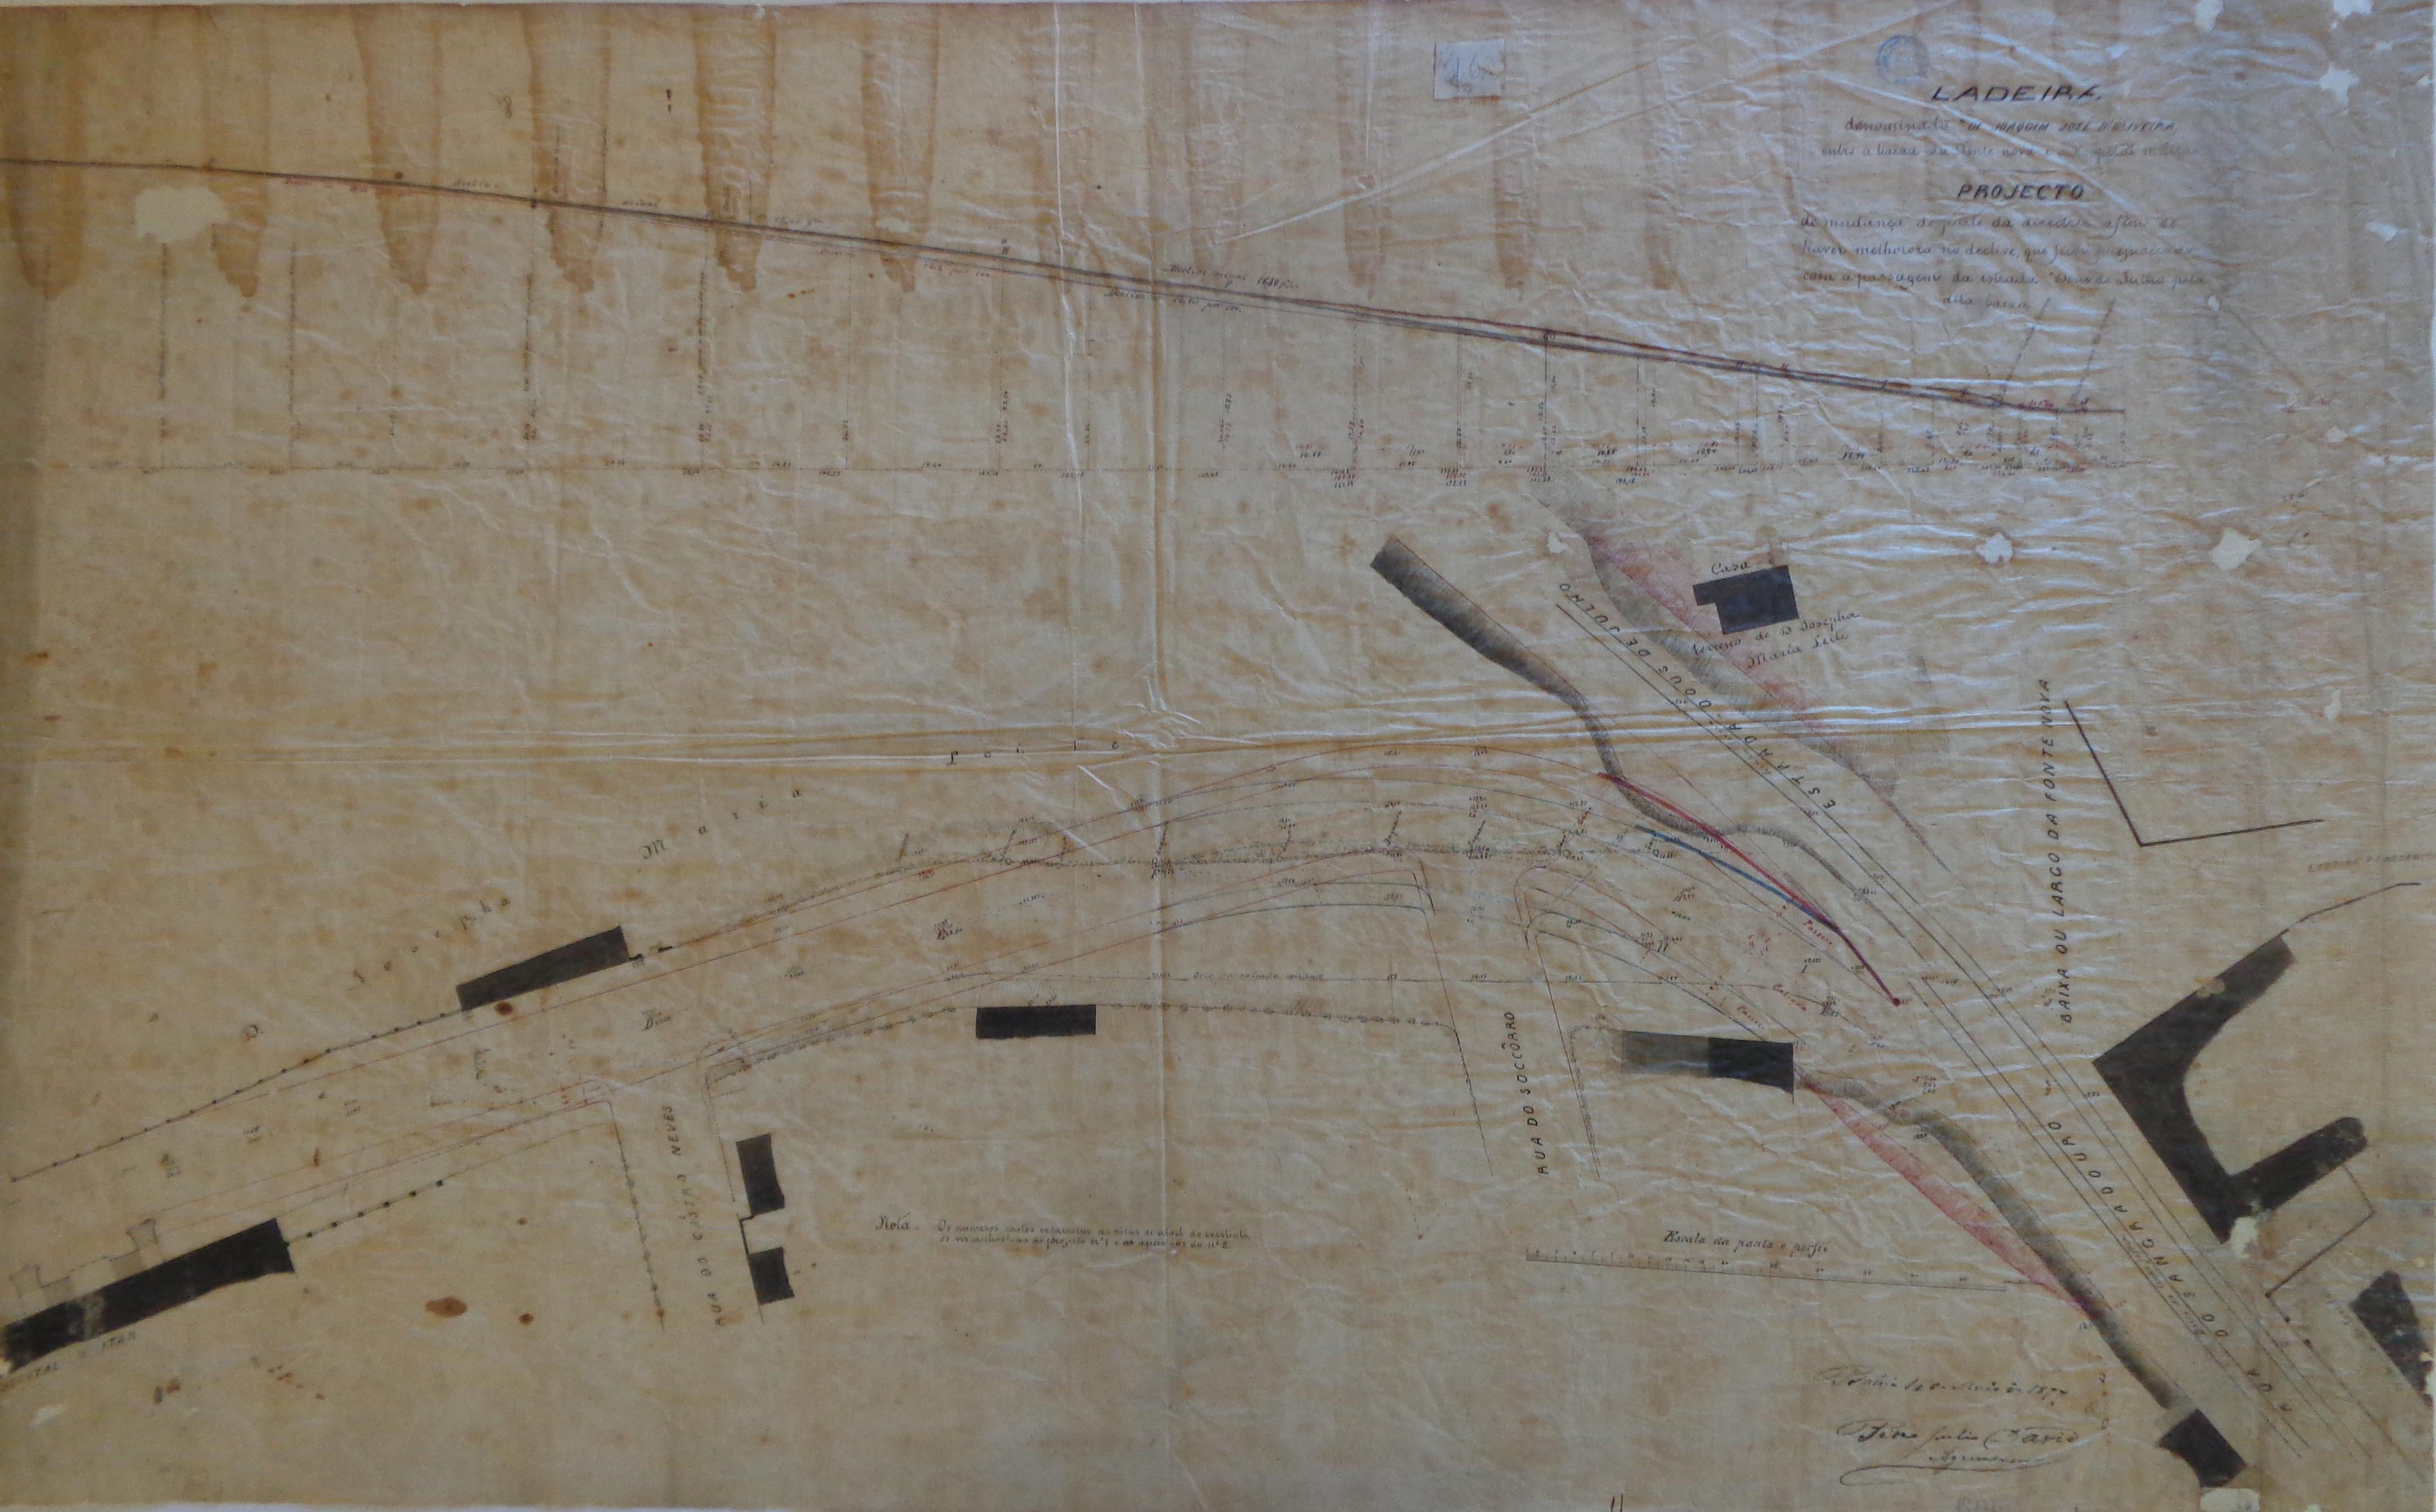
\includegraphics[width=\textwidth]{3-cap2/complementos/mapas/joaquim/joaquim01.eps} 
\label{fig:joaquim01}
}
\caption{Projeto de mudança no declive da ladeira de José Joaquim de Oliveira, de autoria de Pedro Julio David, 1877. \textbf{Fonte:} \textbf{BR BAAPB}, Biblioteca, planta nº 107}
\label{fig:joaquim}
\end{figure}

Observando atentamente o projeto da \autoref{fig:joaquim}, nota-se que a ladeira que ele visa reformar corresponde exatamente à atual ladeira dos Galés.

Outro aspecto notável, a ser visto em maiores detalhes na \autoref{subsubsec:pitangueiras} é que o palacete de Joaquim José de Oliveira foi adquirido pela província da Bahia em 1872 para a construção do \textit{Hospital Militar}, que ainda funciona no mesmo local.

\subsection{A Estrada de Brotas e seus arredores}

\begin{figure}[!htp]
\centering
\subfloat[Em 1851]{
\includegraphics[width=0.4\textwidth]{3-cap2/complementos/mapas/estbrotas-1851.eps} 
\label{fig:estbrotas-1851}
}
\  %espaco separador
\subfloat[Atualmente]{
\includegraphics[width=0.4\textwidth]{3-cap2/complementos/mapas/estbrotas-hoje.eps} 
\label{fig:estbrotas-hoje}
}
\caption{Duas representações cartográficas do território correspondente à Estrada de Brotas (atual av. D. João VI). \textbf{Fonte:} \citeonline{weyll_mappa_1851} e Google Earth.}
\end{figure}

No século XVIII saía do Portão da Piedade uma estrada então conhecida como \textit{Caminho Grande}, correspondente ao que veio depois ser a \textit{Estrada de Brotas}, atual Avenida D. João VI; era por aí que se partia da cidade ao Rio Vermelho, passando pelo paço do Acupe, integrante do morgado da Casa da Torre \cite[p.~85]{campos_brotas_1942}. Patente de sargento-mor da freguesia de ``Nossa Senhora de Brotas do Caminho Grande'' concedida a Veríssimo de Campos de Carvalho em 1725 \cite[p.~114]{texmel_manusbn_1896} mostra como era conhecida a freguesia em seus primórdios.

Infelizmente não foi possível encontrar registros seguros do traçado completo do Caminho Grande, exceto por uma referência que o qualificou como `perigoso'' e disse passar ele ``pela Lapa e atual Campo da Pólvora, pela crista dos montes e pelos divisores de águas, passando em Fonte Nova e por Brotas até aquele ponto da costa oceânica'' \cite[p.~488]{sampaio_salvador_2016}. Com base no mapa de \citeonline{weyll_mappa_1851} (cf. \autoref{fig:estbrotas-1851}), pode-se conjecturar, entretanto, que a ligação entre a Piedade e o atual Largo do Paranhos, onde tinha início a Estrada de Brotas, fosse feita pelo trecho da atual avenida Joana Angélica que vai até a ladeira da Fonte Nova e por esta própria ladeira, chegando, através da atual ladeira dos Galés, até o referido largo, completando assim o primeiro trecho. Daí em diante, pode-se apenas conjecturar, inconclusivamente, por onde o Caminho Grande desceria rumo ao Rio Vermelho.

O jornal quinzenal \textbf{A Lei}, num breve perfil biografico, indicou que em 1848 o brigadeiro Evaristo Ladislau e Silva ``concorreu para o melhoramento da estrada de Brotas''\footnote{\textbf{A Lei}, ano 2, nº 2, fev. 1877, pp. 2-3.}; certamente terá a ver com o fato de que entre 1848 e 1849 a presidência da província investiu 2:269\$344 na Estrada de Brotas, comprometendo-se a investir outros 5:000\$000 em melhoramentos na via; investiu também 1:414\$000 no encanamento do rio Camorogipe, empenhando-se a investir outros 177:539\$000 na mesma finalidade \cite{bahia_rpe_1849}.

Como a Estrada de Brotas era -- e continua sendo, se somarmos as atuais ruas que estão sobre seu antigo leito -- muito comprida, é preciso fazer como os da época e subdividi-la em alguns pontos notáveis e cercanias.

O primeiro deles é o \textit{Largo de Brotas}, existente desde a fundação da igreja matriz. Em 1882 uma casa posta a leilão nesta localidade foi assim descrita e avaliada:

\begin{citacao}
...uma casa ao largo da matriz de Brotas, n. 14, com 5 metros e 46 centimetros de frente, que é dobrada e de azulejos, com porta e 2 janellas, sala feichada, 3 quartos, sala de jantar, cosinha, quintal e sotão, em terreno proprio [\dots]\footnote{\textbf{Diário da Bahia}, 30 set. 1882, p. 3.}.
\end{citacao}

Apesar de um célebre memorialista afirmar que o \textit{largo da Cruz da Redenção}, até hoje existente, foi mandado abrir em 1841 na Estrada de Brotas pelo coronel João Ladislau de Figueredo e Mello, dono do engenho Campinas \cite[p.~88]{campos_brotas_1942}, já se encontra anúncios de venda de roça na mesma localidade em 1838\footnote{\textbf{Correio Mercantil}, vol. 3, nº 583, 19 out. 1838, p. 4.}.

O \textbf{Livro Eclesial de Registro de Terras da Freguesia de Brotas} menciona a existência na localidade de propriedade do sr. José Joaquim de Santa Tereza:



O \textbf{Livro Eclesial de Registro de Terras da Freguesia de Brotas} menciona ainda terreno registrado em nome de Antonio Pereira do Rio:



Rosa Ladislau de Figueiredo e Mello\footnote{Equivocadamente nomeada pelo BR BAAPB como ``Ladislau de Figueiredo Melo'' em seus registros eletrônicos.} era outra a ter terras registradas em seu nome na localidade:




Em 1882 uma casa posta a leilão nesta localidade foi assim descrita e avaliada:

\begin{citacao}
Uma casa situada à rua da Redempção, freguezia de Brotas, com 3 metros e 30 centimetros de frente, e n'esta uma porta e janella, sala, dous quartos, sala de jantar em commum com a cosinha, pequeno quintal; divide-se por um lado com casa do intestado e pelo outro com Luiz Mendes, avaliada por 100\$000\footnote{\textbf{Diário da Bahia}, 3 jan. 1889, p. 2.}.
\end{citacao}



Caetano Vicente de Almeida Galião, juiz de paz do segundo distrito da Sé em 1835, possuía um pequeno engenho e uma pequena fazenda em Brotas \cite[p.~239]{REIS2004males}.

\subsubsection{Cruz das Almas}

O \textbf{Livro Eclesial de Registro de Terras da Freguesia de Brotas} registra a existência, na Cruz das Almas, de uma propriedade do sr. Herculano Nunes dos Reis:



Já em 1870, um certo Miguel dos Santos Prates vinha a público agradecer aos que acompanharam o cortejo fúnebre de seu pai desde sua casa, na estrada da Cruz das Almas, até o cemitério de Brotas\footnote{\textbf{O Monitor}, 20 jun. 1870, p. 3}

No que diz respeito ao \textit{cemitério de Brotas}, antes de caracterizá-lo é preciso desfazer um equívoco historiográfico. Relato de Francisco Vicente Vianna \cite[p.~371]{vianna_bahia_1893} induziu a erro tanto \citeonline{VASCONCELOS2002} quanto \citeonline{flexor_desenho_1999}; segundo \citeauthor{vianna_bahia_1893}, a necrópole teria sido fundada em 1876, mas viu-se na documentação pesquisada que em 1871 este cemitério já demandava ser alargado\footnote{\textbf{Jornal da Bahia}, ano XIX, nº 5.446, 22 set. 1871, p. 1} e que em 1872 ele deixara de funcionar por quatro meses, pelo que se propunha então construir outro cemitério no Acupe \cite[relatório do chefe de polícia, p.~12]{bahia_1872}. Deduz-se de tudo isto que sua fundação ocorreu em data anterior\footnote{\citeauthoronline{flexor_desenho_1999}, com base na Lei do Orçamento Provincial nº 1.131, indica que ``desde 1870 o governo autorizara a compra de um terreno na freguesia de Brotas, em frente da Cruz da Redenção, para estabelecer um cemitério público'', mas diz, imediatamente em seguida, que ``a reação contra os enterramentos, fora ou longe das igrejas, retardou a iniciativa'' (\citeyear{flexor_desenho_1999}, p. 104), deixando a data de fundação do cemitério como 1876.}, mas nem a documentação pesquisada nem a bibliografia consultada permitiram precisá-la em definitivo. O que de fato ocorreu em 1876 naquele cemitério foi que no dia 4 de julho o juiz e mesário da irmandade do Santíssimo Sacramento de Nossa Senhora de Brotas requereu ao administrador do cemitério 30 metros quadrados de terreno devoluto para a construção de carneiros para a irmandade\footnote{\textbf{O Monitor}, 16 jul. 1876, p. 2}. Em 1879 a presidência da província transferiu a administração do cemitério para a Câmara Municipal por meio da lei 1.943, de 26 de agosto do mesmo ano\footnote{\textbf{O Monitor}, 30 ago. 1879, p. 1.}. Relatórios anuais de governadores provinciais indicam estar esta necrópole sempre em bom estado de conservação e asseio.

\subsubsection{Estrada e Alto do Beijú}

O \textbf{Livro Eclesial de Registro de Terras da Freguesia de Brotas} menciona a existência de terrenos registrados em nome de Bernardino José de Almeida, assim descritos:




\subsection{A fazenda Boa Vista e seus arredores}

\begin{figure}[!htp]
\centering
\subfloat[Em 1851]{
\includegraphics[width=\textwidth]{3-cap2/complementos/mapas/boavista-sangradouro-1851.eps} 
\label{fig:boavista-sangradouro-1851}
}
\  %espaco separador
\subfloat[Atualmente]{
\includegraphics[width=\textwidth]{3-cap2/complementos/mapas/boavista-sangradouro-hoje.eps} 
\label{fig:boavista-sangradouro-hoje}
}
\caption{Duas representações cartográficas do território correspondente à fazenda Boa Vista (atual Engenho Velho de Brotas) e ao Sangradouro (atual Santo Agostinho). \textbf{Fonte:} \citeonline{weyll_mappa_1851} e Google Earth.}
\end{figure}

O Livro... registra três herdades na localidade, a saber:




Merece nota também a fazenda \textit{Engenho Velho}:

\begin{citacao}
Medição da fazenda denominada Engenho Velho na freguesia de Brotas desta cidade, pertencente a Dona Anna Francisca de Carvalho, viúva do finado Antonio Teixeira de Carvalho, contendo de frente quatrocentas e trinta braças e de fundo cento e vinte e cinco; divide com terras do finado Padre João Thomas da parte do nascente, tendo por divisa um [\textit{ilegível}] aonde tem cerca nativa pertencente tudo à mesma fazenda, e pelo poente divide com terras da viúva Dona Leonarda Ramos por huma cerca nativa, e pelo vertente dividindo com terras de hum negociante Gantois pelo rio corrente, contendo na mesma fazenda huma casa de campo e huma porteira de pedra e cal de quatro braças de frente e [\textit{ilegível}] de fundo qua[\textit{ilegível}], com grande número de árvores de espinhos e [\textit{ilegível}] toda a terra [\textit{ilegível}]. Bahia e Engenho Velho, oito de julho de mil oitocentos e cincoenta e oito. Anna Francisca de Carvalho. E nada mais continhão as declarações que me forão enviadas. Brotas da Bª, 10 de julho de 1858.
Vigº Ernesto de Olivª Valle.\footnote{\textbf{BR BAAPB}, fundo Colonial, série Registros de Terra, livro 4675, f. 23 verso.}
\end{citacao}

O mapa de \citeonline{weyll_mappa_1851} mostra ainda uma longa estrada saindo das terras da Boa Vista em direção a uma estrada que corresponde à atual avenida Cardeal da Silva. Remanescentes desta estrada são as ruas Almirante Alves Câmara e Padre Luiz Figueira, no Engenho Velho de Brotas, e Sérgio de Carvalho, no Vale da Muriçoca; mais ou menos no ponto onde a Sérgio de Carvalho faz esquina com a atual av. Edite, também no Vale da Muriçoca, o mapa de Weyll indica uma ponte sobre um riacho, e daí em diante a estrada seguia um curso hoje inexistente, que terminava aproximadamente na altura da atual Ladeira das Carmelitas, na Federação. Seria esta a Estrada da Boa Vista, estendendo-se desde o Largo dos Paranhos até a atual Cardeal da Silva? Difícil dizer, dado que em 1851 esta área era eminentemente rural. Por outro lado, o \textbf{Atlas parcial da cidade do Salvador}, mandado publicar pela Prefeitura de Salvador em 1955, apresenta uma configuração toponímica e física do Engenho Velho de Brotas muito próxima daquela encontrada durante a Primeira República\footnote{Só foi possível utilizar o \textbf{Atlas parcial da cidade do Salvador} a contento na medida em que suas informações foram cotejadas com a documentação pesquisada e com o mapa de \citeonline{weyll_mappa_1851} (cf. \autoref{fig:atlasenvgelho1955}); trata-se de documento produzido muito posteriormente ao período estudado, quando já se haviam verificado grandes modificações no tecido urbano de Brotas por força da intensificação da urbanização ocorrida no distrito durante a era Vargas (1930-1945). No que diz respeito a toponímicos e a localizações aproximadas de pontos notáveis, entretanto, trata-se de fonte documental preciosíssima, desde que, ressalte-se ainda outra vez, cotejado com outras fontes e documentos para estabelecer o que dele se aproveita e o que dele é posterior ao período pesquisado.}; nele, interessam particularmente os seguintes aspectos:

\begin{figure}[!htp]
\centering
\includegraphics[width=1\textwidth]{3-cap2/complementos/mapas/apcs1955-f32-engvbro.eps} 
\caption{Folha 32 do \textbf{Atlas parcial da cidade do Salvador}. O Engenho Velho de Brotas é a área acima do Dique do Tororó. \textbf{Fonte:} \citeonline{municipal_atlas_1955}.}
\label{fig:atlasenvgelho1955}
\end{figure}

\begin{enumerate}
\item A atual rua Brígida do Vale corresponde à região circunvizinha à Capela do Deus Menino, que, a julgar pela documentação consultada e por duas obras de referência pesquisadas \cite{municipal_atlas_1955,souza_guia_1935}, teve vários toponímicos ao longo do tempo (Rua da Capelinha, Alto da Capelinha etc.).
\item A rua denominada na documentação encontrada como Monte de Belém é na verdade o topônimo de uma pequena área, e na verdade divide-se em três (Monte Belém de Cima, Monte Belém de Baixo, Monte Belém do Meio); estas ruas, que mantiveram estes nomes até hoje, situam-se na encosta adjacente à atual rua Brígida do Vale.
\item A Vila América e o Alto do Moinho, encontrados na documentação pesquisada, são duas pequenas localidades vizinhas situadas numa encosta que dá de frente para a atual avenida Vasco da Gama.
\item A julgar pela comparação entre o \textbf{Atlas} e a documentação pesquisada, a atual ladeira da União (também conhecida como Estrada da União) já era conhecida por este topônimo desde pelo menos o final do século XIX, e era adjacente ao porto dos Saveiros, no Dique do Tororó.
\item Próximo ao canto superior esquerdo do mapa pode-se ver o Dique Pequeno, constante na documentação pesquisada e hoje aterrado, correspondente à área onde hoje se situam a rua Jornalista Archimedes Gonzaga e a rua Dique Pequeno.
\end{enumerate}









\subsection{A Estrada Dois de Julho}

\begin{figure}[!htp]
\centering
\subfloat[Em 1851]{
\includegraphics[width=0.7\textwidth]{3-cap2/complementos/mapas/e2j-1851.eps} 
\label{fig:e2j-1851}
}
\  %espaco separador
\subfloat[Atualmente]{
\includegraphics[width=0.7\textwidth]{3-cap2/complementos/mapas/e2j-hoje.eps} 
\label{fig:e2j-hoje}
}
\caption{Duas representações cartográficas da Estrada Dois de Julho (atual av. Vasco da Gama). Em 1851 ela não estava construída, mas corresponde ao leito do rio Lucaia. \textbf{Fonte:} \citeonline{weyll_mappa_1851} e Google Earth.}
\end{figure}

A Estrada Dois de Julho, hoje conhecida como avenida Vasco da Gama, foi inaugurada em 1859 como caminho alternativo entre o arrabalde do Rio Vermelho e a zona urbana de Salvador; seu trajeto corre rente ao rio Lucaia, desde sua nascente no Dique do Tororó até as vizinhanças da sua foz, no Rio Vermelho \cite[p.~582]{ruy_politica_1949}.

Em 31 de março de 1877 a Câmara Municipal pediu providências quanto aos aterros no Dique do Tororó promovidos durante o ``assentamento dos trilhos da linha férrea do Rio Vermelho'', pois ``as águas alli estagnadas têm causado damno à saude publica, produzindo febres intermittentes e perniciosas nos moradores das Pitangueiras, Matatú, Castro Neves e Bôa-Vista''\footnote{\textbf{Correio da Bahia}, ano VII, nº 12, 10 abr. 1877, p. 2}.

Em 10 de maio de 1879 o presidente da província ordenou ao diretor de obras públicas 

\begin{citacao}
\dots lavrar contracto n'essa repartição com o Commendador Giusto Ariani para o serviço de deseccação do terreno na estrada Dous de Julho, entre a fábrica de lapidação de diamantes pertencente aos negociantes Costa Pinto \& Filhos e a ladeira que segue para Brotas, e bem assim para a canalisação da parte do riacho Lucaia entre aquelles dous pontos\footnote{\textbf{O Monitor}, 3 jun. 1879, p. 1.}.
\end{citacao}



\subsection{O Matatu Grande, o Matatu Pequeno, Quinta das Beatas e arredores}\label{subsec:matatubeatas}

Em 17 de junho de 1799 o Conselho Ultramarino deu parecer favorável a requerimento de porte de armas defensivas feito pelo capitão Pedro Gomes Ferreira; o militar residia ``na sua fazenda do Matatu'' \cite[p.~228]{castralmeida_ultramar_1914}, indicando que já no século XVIII a área era reconhecida por este nome. 

Há duas versões para a etimologia do topônimo. A primeira e mais conhecida diz ser ele de origem tupi, significando ``mata escura'', ``floresta negra'' \cite[p.~281]{sampaio_tupi_1987}. A segunda, menos conhecida, diz que se trata de um africanismo de origem bantu, significando ``lugar deserto, isolado'' \cite[p. 46]{dorea_ruas_2006}. Qualquer das duas versões, seja pela existência de mata fechada, seja escassez populacional, passam a impressão de um lugar distante, ermo, pouco povoado, e é bem possível que assim o fosse no século XVIII quando encontramos a primeira referência ao nome; no século XIX, entretanto, o \textbf{Livro Eclesial de Registro de Terras da Freguesia de Brotas} indica a existência de muitos pequenos proprietários de terras na área, sendo ela a que mais tem registros fundiários em toda a freguesia\footnote{\textbf{BR BAAPB}, fundo Colonial, série Registros de Terra, livro 4675.}.

No mapa de \citeonline{weyll_mappa_1851}, lido no sentido NNE-SSE (cf. \autoref{fig:matatu-1851}), a área é representada por três cumeadas. 

\begin{figure}[!htp]
\centering
\subfloat[Em 1851]{
\includegraphics[width=0.7\textwidth]{3-cap2/complementos/mapas/matatu-1851.eps} 
\label{fig:matatu-1851}
}
\  %espaco separador
\subfloat[Atualmente]{
\includegraphics[width=0.7\textwidth]{3-cap2/complementos/mapas/matatu-hoje.eps} 
\label{fig:matatu-hoje}
}
\caption{Duas representações cartográficas do Matatu, mostrando a rua da Valla (atual av. Heitor Dias), a Estrada da Pólvora (atual rua Raul Leite), a Estrada do Matatu Grande (atual rua Luiz Anselmo) e a Quinta das Beatas (atual Cosme de Farias). \textbf{Fonte:} \citeonline{weyll_mappa_1851} e Google Earth.}
\end{figure}

A terceira tem uma estrada, correspondente à atual rua Cosme de Farias, que vai dar na ``Quinta das Biatas''
 
No mesmo mapa é possível encontrar símbolos indicativos de construções pontilhando a cumeada do Matatu Grande, embora a cumeada onde se localiza a Casa da Pólvora apresente-se pouco povoada, assim como a da Quinta das Beatas.

Novamente lendo o mapa de Weyll no sentido NNE-SSE (\autoref{fig:matatu-1851}), quatro rios escavam os vales circundantes destas cumeadas; todos já foram caracterizados na \autoref{}. 

Dado o grande tamanho da área analisada, será preciso subdividi-la nos pontos notáveis e nomes pelos quais era conhecida na época, atualizando-os quando necessário.

\subsubsection{Largo do Paranhos: porta de entrada para Brotas}

A porta de entrada para o Matatu, no sentido de quem vem da Ladeira dos Galés, é o \textit{largo do Paranhos}, assim batizado em homenagem ao já mencionado latifundiário Tomás da Silva Paranhos.

Em 1879 foi anunciado o leiloamento de uma roça de propriedade de Herman e Sophia Both, penhorada pela Sociedade de Commercio, localizada no largo do Paranhos, descrita no anúncio a seguir. Observe-se com detalhe a estrutura e o valor do imóvel à venda; trata-se de fazenda bem constituída, de gente abastada o suficiente para ter inquilinos:

\begin{citacao}
Uma roça em terreno proprio, na freguezia de Brotas, largo denominado de Paranhos, tendo a frente para o mesmo largo, dividindo-se pelo lado direito com a roça que foi do Bacharel Firmino Duarte Gameleira; pelo esquerdo, com a estrada que vai para a Quinta das Beatas; e pelo lado direito continuando de fundo à frente com terreno que foi do dito Bacharel Gameleira onde vae acabar. Medida a frente da roça, acha-se n'ella 336m 10c; do canto que vira para a estrada da Quinta das Beatas até encostar na roça que foi do Bacharel Gameleira, havendo n'este lado 143m 60c; de terreno, com o fundo de 43m 25c, que foram dados por aforamento a diversos, pelos executados, de modo que fica a frente propriamente dita da roça com 180m 50c, desde o terreno aforado até a esquina para a estrada das Boiadas, e essa frente está fechada por muros de boa construcção, tendo um portão de ferro por onde é a entrada principal para a roça e casa de morada. A entrada do portão para a casa é guarnecida de perfeitas cercas de pitangueiras, que terminam em 2 carramanchões sobre pilastras de pedra de cantaria; dentro das cercas de pitangueiras existem diversas arvores, como saputizeiros, abacateiros, laranjeiras etc., havendo no lado esquerdo da mesma roça diversas divisões formadas por cercas de pitangueiras, e em todos esses lotes diversas arvores, como as declaradas, cuja quantidade é a seguinte:

Na parte cultivada da roça existem: 60 jaqueiras, 73 mangueiras, 193 laranjeiras, 10 pes de fructa pão, 8 cajazeiras, 8 abacateiros, 24 saputizeiros, 23 coqueiros, 2 genipapeiros, 1 tamarindeiro, 4 [ilegível] de parreira, sendo algumas de pés direitos de cantaria, 1 brejo que termina em uma ribanceira, onde existe uma capoeira para corte de madeira, 1 telheiro fechado por paredes de taboas com uma machina à vapor em bom estado, serve para conduzir agua a um deposito junto á propriedade da morada, a qual agua é puxada por um encanamento de ferro, de um deposito de pedra e cal cimentado e coberto tambem com telheiro, 1 banheiro fechado por paredes de pedra e cal, e coberto de telhas, com 2 portas e 3 torneiras de bronze.

Uma casa de campo de gosto antigo com varandas fechadas por frontoes, e n'elles peitoris, tendo no lado direito da varanda, 1 oratorio de celebrar missa. A entrada é por uma porta entre 4 janelas, com sala aberta que occupa a porta e 2 janelas, e 1 gabinete em cada lado, tendo cada gabinete 1 janella, e a entrada para o interior da casa é pela sala de jantar que dá em 1 salão, havendo de cada lado deste 1 corredor, com diversos repartimentos que são: 10 quartos, dispensa e cozinha, toda construida de pedra e cal e de gosto antigo. Depois desses repartimentos um grande salão de pedra e cal, com paredes dobradas, feito muito depois da casa, e de gosto moderno, rodeado de janellas de vidraças, isto é, com janelas de vidraças no fundo e no lado, e a parte por onde abre-se para um terraço d'onde desce-se para o centro da roça por uma escada de pedra, sobre este salão há um sotão para onde sobe-se por uma escada interna, tendo o mesmo sotão 4 divisões eguaes (4 grandes quartos ou 4 pequenas salas) cada uma com 2 janelas de vidraças, pelo que é o dito sotão rodeado de janellas, tanto a sala da frente como os quartos e o salão são forrados; a sala e os mais commodos terreos são cimentados, e o sotão é de lages de pedra; a casa descripta e o seu acrescimo (salão e sotão) tem de frente 12m60c de comprimento de frente a fundo 38m30c, cinco senzalas cobertas de telha em estado de reparo, dentro da roça, com 25m90c de frente; e em seguimento as mesmas senzalas 2 cazinhas que estão alugadas, e cujos inquilinos aproveitam-se na entrada e sahida do porão da cocheira.

Em frente ás senzalas e encostado ao muro da roça, existe um grande armazem, onde foi antiga estribaria, que ainda hoje tem em parte mangedouras, armazem esse que é coberto de telhas e precisa de reparos. A roça, casa e mais dependencias as avaliaram em 10:000\$000 [\dots]\footnote{\textbf{O Monitor}, 10 dez. 1879, p. 2.}.
\end{citacao}

\subsubsection{Pitangueiras: um povoado nobre}\label{subsubsec:pitangueiras}

Passado o largo do Paranhos, chega-se de imediato à estrada que os contemporâneos chamavam das \textit{Pitangueiras}, curto trecho entre o largo e a estrada do Matatu Pequeno, hoje conhecida como Rua Barros Falcão. 

Já em 1851 o \textbf{Livro Eclesial de Registro de Terras da Freguesia de Brotas} registrava terras em nome do padre Felisardo Jerônimo Soares, a saber:

\begin{citacao}
O abaixo assignado possue na freguesia de Brotas e logar denominado Pitangueiras um terreno com sete braças de frente na mesma estrada de Brotas e cinco de fundo, que ficam na travessa, que vae da mesma estrada para a do Matatú, onde confina com terras de Francisco de Assis Gomes, confinando pelo lado do sul com terras do dito Assis, e do Capitam Salvador Pires de Carvalho e Albuquerque, tendo obtido este terreno por compra que fez a Marinha Rodrigues da Silva. Bahia, vinte e um de junho de mil oitocentos e cincoenta e oito. O Padre Felisardo Jerônimo Soares. E nada mais continhão as declarações [\textit{ilegível}] Brotas da Bª, 30 de junho de 1858. 
Vigº. Ernesto de Olivª Valle\footnote{\textbf{BR BAAPB}, fundo Colonial, série Registros de Terra, livro 4675, f. 16 verso.}
\end{citacao}

Outro proprietário de terras nas Pitangueiras era José Joaquim de Santa Tereza:

\begin{citacao}
Terra que comprou José Joaquim de Santa Tereza a Domingos José Cardozo no lugar denominado Pitangueiras, freguesia de Nossa Senhora de Brotas da Bahia, com tres braças de frente divide pelo norte com o próprio comprador pelo lado opposto com o Capitão Salvador Pery de Carvalho e pelo fundo com o padre Feliciano Jeronimo Soares. Brotas, dezesseis de julho de mil oitocentos e cincoenta e oito. José Joaquim de Santa Tereza. E nada mais continhão as declarações que me forão dadas. Brotas da Bª, 17 de julho de 1858{\textbf{BR BAAPB}, fundo Colonial, série Registros de Terra, livro 4675, f. 31 frente.}.
\end{citacao}

Este senhor José Joaquim de Santa Tereza chamou a atenção pelo fato de encontrarmo-lo, anos depois, em meio às licenças de construção e reforma do \textbf{Arquivo Histórico Municipal de Salvador}, embora já falecido, como ex-proprietário de um dos imóveis reformados, então de propriedade de seu legatário Roberto da Trindade de Jesus. Busca no \textbf{Arquivo Público da Bahia} revelou ainda existirem lá custodiados os autos de seu inventário, onde há fatos muito interessantes. Este senhor, rico porém analfabeto, além de deixar várias casas na rua do Cabral e na rua do Jogo do Carneiro (freguesia de Sant'Anna) para seu afilhado, parentes e escravos alforriados, outras tantas casas na rua da Paciência (Rio Vermelho) para seus amigos, quantias variadas para moradores da armação do Saraiva e de Itapuã e de deixar rendas e usufrutos para a Irmandade de Nossa Senhora do Santíssimo Sacramento e do Rosário de Brotas, legou a Izidra Prima de Jesus, irmã de seu afilhado Martiniano Primo de Jesus, uma casa térrea nas Pitangueiras, e a seu amigo Francisco Lopes Fiuza uma casa no largo de Brotas; descontados estes e uma grande quantidade de outros bens, rendas e pagamentos, e na ausência de herdeiros naturais, sobraram-lhe ainda bens suficientes para legar a Roberto da Trindade de Jesus como seu ``presumptivo e universal herdeiro'' e deixá-lo com uma relativa fortuna\footnote{\textbf{BR BAAPB}, fundo Judiciário, seção Inventários, estante 7, caixa 2989, documento 2.}. Em momento oportuno voltaremos a falar da fortuna deste herdeiro. 

Em 1863 Pitangueiras foi uma das localidades escolhidas para receber alguns dos 347 combustores de iluminação a gás que restavam para completar os 2 mil contratados com a presidência da província da Bahia \cite[p.~52]{bahia_rpe_1863}. Disto resultou um fato curioso: instalados os combustores, um indivíduo começou a apagá-los; preso e conduzido à presença do presidente da província, confessou que era acendedor de lampiões nas Pitangueiras e apagava-os por ordem do fiscal da empresa responsável pela iluminação pública assim que se mostravam ``amortecidos'', pois a multa cobrada pela polícia pelos amortecidos e pelos apagados era igual e os ``amortecidos'' -- ou seja, com iluminação fraca -- ainda consumiam gás \cite[relat.~chefe~polícia,~p.~25]{bahia_rpe_1870}. 

Ficava nas Pitangueiras o ``predio nobre'' pertencente aos herdeiros do coronel Antonio José de Lima, comprado pelo Ministério da Guerra em 1872 para a instalação do Hospital Militar \cite[p.~30]{bahia_1872}, ainda hoje existente (embora ``prédio nobre'' tenha sido demolido em uma de suas reformas). Tratava-se do antigo palacete de Joaquim José de Oliveira \cite[p.~36]{bahia_rpe_1874}, que por caminhos comerciais ou sucessórios fora parar em mãos de Antonio José de Lima, depois de seus herdeiros e por último com a província. A aquisição, um investimento de 70:000\$000 \cite[p.~10]{bahia_1872}, foi saudada por estarem ``attendidas as condições essenciaes de um bom hospital'': ``vastidão, solidez, bella e saudavel situação, proximidade do interior da cidade, servido pela linha de \textit{Trilhos Centraes} e em um bairro muito procurado'' \cite[p.~31]{bahia_1872}.

Em 1871 uma escola primária masculina havia sido recentemente removida para este povoado, medida elogiada pelo rápido crescimento das turmas e pela abertura de turmas noturnas para artistas-operários\footnote{\textbf{Jornal da Bahia}, ano XIX, nº 5.445, 21 set. 1871, p. 1.}; tal remoção, entretanto, teria prejudicado os moradores do largo de Brotas, que só em 1876, depois de muito peticionar ao governo provincial (ao que parece muito contente com a medida, pois registrou haver duplicado o número de alunos depois dela \cite[relat.~instrução~pública,~p.~25]{bahia_1872}), conseguiram deste a contratação de professores particulares para meninos e meninas da localidade\footnote{\textbf{O Monitor}, 3. set. 1876, p. 1.}. A situação, entretanto, ainda não havia melhorado em 1877, como se vê neste clamor assinado por um ``Amigo das Letras'':

\begin{citacao}
\textbf{Aos senhores deputados provinciaes}

Pedimos aos senhores deputados provinciaes que se dignem lançar suas vistas sobre a freguezia de Brotas desta capital, que muito necessita de duas escolas, sendo uma para cada sexo. As cadeiras dessa freguezia acham-se funcionando no logar denominado Pitangueiras -- de forma que um grande numero de crianças de um e outro sexo que moram no largo de Brotas e no Engenho Santo Antonio não podem receber a instrucção primaria.
Bahia, 18 de março de 1877\footnote{\textbf{O Monitor}, 22 mar. 1877, p. 3.}.
\end{citacao}

Ainda em abril de 1877 a situação da escola em Pitangueiras parecia periclitante, pois sua transferência para um extremo da freguesia resultara em grande evasão escolar\footnote{\textbf{O Monitor}, 28 abr. 1877, p. 1.},

Não é difícil deduzir desta situação que Pitangueiras era localidade de difícil acesso para os moradores do largo de Brotas e do Engenho Santo Antônio; pode-se igualmente deduzir, embora com menor certeza, a hipótese de que estas duas últimas localidades tivessem, entre 1871 e 1877, número de moradores maior que o de Pitangueiras. 

É certo, entretanto, que já em 1879 Pitangueiras concentrava razoável infraestrutura urbana, pois anúncio de casa a alugar nesta localidade indicava ter a mesma ``os commodos necessarios para familia e encanamento de gaz''\footnote{\textbf{O Monitor}, 17 maio 1879, p. 2.}. Na mesma linha vai o anúncio de leiloamento dos seguintes imóveis, todos de bom padrão para a época:

\begin{citacao}
\textbf{Bens de raiz -- }Uma casa abarracada sita à rua das Pitangueiras, freguesia de Brotas, de n. 159, edificada em terreno proprio, com 8 metros e 10 centimetros de frente e 24 metros e 10 centimetros de fundo que dá para a rua Sete de Setembro, tendo de lado que dá para o beco 18 metros e 80 centimetros, com terraço na frente com gradil de ferro; a casa tem 2 janellas de peitoril e porta de vidraça no centro, 5 janellas do lado, sala de espera com porta para o becco, sala de visita, 2 quartos, salla de jantar e dispensa, e toda ella forrada, salla de gommar e cozinha, 3 quartos no quintal, lenheiro e sofás de cimento e concha para recreio, quintal todo murado com um portão para a dita rua, sotão com sala e 3 quartos, paredes todas dobradas, divide-se por um lado com casa do mesmo casal, avaliada por 4:000\$000.

Uma casa abarracada sita na dita rua e freguezia, de n. 157, edificada em terreno proprio, com 7 metros e 80 centimetros de frente com terraço e gradaria de ferro, com 2 janellas e porta no centro, sala de frente, 3 quartos, sala de jantar e toda ella forrada, dispensa, cozinha, sala de gommar com 2 quartos no quintal, sotão com janellas para a frente e fundo, com sala e 3 quartos, quintal todo murado com porteira para a rua Sete de Setembro, divide-se a casa por outro lado com casa do casal, avaliada por 3:000\$000.

Um terreno sito à rua Sete de Setembro, na dita freguezia, tendo de comprimento 38 metros, dividindo-se pelo fundo com terrenos do Hospital Militar, tendo diversas casas n'elle edificadas, avaliado cada metro por 15\$000 e todos por 570\$000 [\dots]\footnote{\textbf{O Monitor},3 out. 1879, p. 2.}.
\end{citacao}

O intérieur das habitações das Pitangueiras era rico e bem ornamentado, como se pode ver a partir deste anúncio:

\begin{citacao}
Leilões [\dots]

Luiz Zuanny 

Venderá em leilão na terça-feira 2 de dezembro (dia desoccupado) às 11 horas em ponto na chácara as Pitangueiras, estrada do Matatú, freguezia de Brotas, por conta de quem pertencer, o seguinte: mobília de jacarandá, dita de Gonçalo Alves, mobilias autriacas, um piano de Pleyel n. 4 quasi novo, tapetes, escarradeiras, jarras finas de Bacarat, figura de Biscuit, quadros a oleo, espelho com grande moldura dourada, ditos pequenos, um lustre de cristal de 6 luzes, ditos de 3 e 2 luzes, arandellas de cristal e metal, tudo para gaz, cantoneiras, venesianas, pannos de crochet e de renda para cadeiras, etc., uma importante mobilia de quarto de Gonçalo Alves a Luiz XV, composta de cama, toilete e lavatorio, retrete e dous guarda-vestidos, uma pequena mobilia de Gonçalo Alves para gabinete, sendo o sofá e 8 cadeiras a Luiz XV obra moderna, cortinado de crochet para cama, cantoneiras com pedra marmore, uma grande mesa de vinhatico para jantar, guarda-louças, com etagéres, quartinheiro, guarda-comidas, cadeiras de vinhatico, dita de vimes, apparelho de porcellana para jantar, dito para almoço, copos, calices, garrafas, compoteiras, fructeiras, bandeijas, trem de cosinha, etc., etc., etc.

\textbf{Attenção}

No mesmo dia às 2 horas da tarde se vendera a importante chácara com excelente casa de morada e dependencias, grande jardim com gradil de ferro, brejo, plantação de capim e porção de arvoredos fructíferos etc.\footnote{\textbf{Gazeta da Bahia}, ano I, nº 267, 25 nov. 1879, p. 2}.
\end{citacao}

\subsubsection{Quinta das Beatas: especulação imobiliária e ordens religiosas}

Passado trecho da estrada das Pitangueiras, chega-se a uma esquina onde se abre a estrada que conduz à \textit{Quinta das Beatas}. A fazenda que ficou conhecida por este nome, no atual bairro de Cosme de Farias, tem sua descrição no \textbf{Livro Eclesial de Registro de Terras da Freguesia de Brotas} extremamente danificada pela ação do tempo:

\begin{citacao}
Quinta das Beatas

[\textit{ilegível}] fazenda denominada Quinta das Beatas é propriedade do Recolhimento do Senhor Bom Jesus dos [\textit{Perd}]oens, está situada na freguesia de Nossa Senhora [\textit{de}] Brotas, confina pelo nascente com a fazenda de[\textit{no}]minada Campina, dos herdeiros do coronel João Ladis[\textit{la}]u de Figueredo, e Matatu Grande, pertencente ao [\textit{ilegível}] Pinto, pelo poente com a roça do tenente[\textit{-coron}]el Pinheiro e com o capitão Paranhos, pelo sul [\textit{com}] a roça de Amorim Vianna, com a Torre e com a [\textit{ilegível}] e pelo norte com o Matatu pequeno e com [\textit{ilegível}] [\textit{ilegível}] Paranhos. Bahia, dezesseis de março de [\textit{mil oitocentos e}] sessenta. Anna Maria Magdalena Re[\textit{jente}]. 

[\textit{E nada mais}] se continha em as ditas declarações [\textit{que me for}]am enviadas.

Brotas da Bª, 20 de [\textit{março de 1860}].

Vigº Ernesto de Olivª Valle\footnote{\textbf{BR BAAPB}, fundo Colonial, série Registros de Terra, livro 4675, f. 40 verso.}
\end{citacao}

A antiga sede da fazenda, a julgar pelo que mostra o mapa de \citeonline{weyll_mappa_1851}, estaria em algum lugar no trecho da atual rua Cosme de Farias situado entre as esquinas das atuais ruas Jaguarari e Lima Durval.

A relação entre o Recolhimento dos Perdões e a Quinta das Beatas é um dos mais acabados exemplos do \textit{rentismo}, sustentáculo econômico de tantas ordens religiosas católicas desde a fundação de Salvador até o presente. Na tentativa de fazer subir sua ordem na hierarquia eclesial (de \textit{recolhimento} a \textit{casa de professas}), mais especificamente como parte da ordem das carmelitas calçadas, as irmãs recolhidas nos Perdões argumentaram por todos os meios possíveis, incluindo os econômicos; em 1820 alegaram possuir, além do 

\begin{citacao}
recato e honestidade em que vivião, o possuirem renda sufficiente de 28 predios urbanos, a grande roça de nossa Sra. da Conceição das Brotas, mais conhecida por \textit{quinta das beatas}, não pequena porção de terreno arrendado e aforado, além de 16:000\$000 rs. em dinheiro de varios legados [\dots] \cite[p.~231]{accioli_memorias5_1937}.
\end{citacao}

Embora o relato apresente mais uma das tentativas frustradas de ascensão hierárquica das recolhidas, deixou evidente seu poder econômico. Pequeno, se comparado ao dos beneditinos, por exemplo \cite{bento_tombo_1945}, mas, mesmo assim, \textit{poder}. Veja-se, como exemplo, dois terrenos aforados mencionados no \textbf{Livro Eclesial de Registro de Terras da Freguesia de Brotas}

\begin{citacao}

\end{citacao}

\subsubsection{Ladeira do Fabrício: inovação e enobrecimento}

Por ser de 1851, o mapa de Weyll ainda não poderia mostrar a \textit{Ladeira do Fabrício}, conhecida a princípio como \textit{Estrada do Sangradouro ao Matatu}, que corresponde ao trecho que inicia na Rua dos Tupys, esquina com a atual Rua do Sangradouro, e segue pela Ladeira dos Bandeirantes até encontrar-se com a estrada para o Matatu no local onde hoje a Ladeira dos Bandeirantes faz encruzilhada com as atuais ruas Alberto Torres, Barros Falcão e Amazonas. 

Esta ladeira foi mandada abrir em 1876 pelo governo provincial, em obras supervisionadas por uma comissão ``composta do Tenente-Coronel Fabricio Alves de Araujo, Bacharel Firmino Duarte Pacifico Gameleira e Negociante Manuel da Silva Pereira Guimarães'' \cite[p.~23]{bahia_1878}. A obra já se encontrava concluída no ano seguinte, sendo alargada de seus 8,8m originais para a largura de 11m e tendo recebido na mesma ocasião ``declives menos fortes'' \cite[p.~228]{bahia_1879}, e em 1885 recebeu calçamento \cite[p.~11]{bahia_1885}.

\subsubsection{Matatu Grande e Matatu Pequeno: fragmentação imobiliária}

Passada a entrada da Quinta das Beatas, a estrada das Pitangueiras segue adiante até surgir uma bifurcação entre a \textit{Estrada do Matatu Grande} (direita) e a \textit{Estrada do Matatu Pequeno} (esquerda)\footnote{Há indicação de que a Estrada do Matatu Grande corresponderia às atuais ruas Luiz Anselmo e Raul Leite, e a Estrada do Matatu Pequeno à atual rua Barros Falcão \cite[p.~124]{valladares_beaba_2012}; a indicação, entretanto, não faz sentido, porque a junção da Luiz Anselmo com a Raul Leite resultaria numa grande via, em forma aproximada de ``U'', que reuniria as cumeadas dos morros que no mapa de \citeonline{weyll_mappa_1851}, contemporâneo das antigas denominações, são separadas como ``Matatu Grande'', à direita, e ``Casa da Povora'', à esquerda. Na falta de documentos comprobatórios da mudança toponímica, não encontrados até onde foi possível avançar na pesquisa ora exposta, parece muito mais plausível que a Estrada do Matatu Grande corresponda à rua Luiz Anselmo e a Estrada do Matatu Pequeno à rua Raul Leite.}.

O \textit{Matatu Grande} situa-se ao final de uma estrada que corresponde em grande parte à atual Rua Luiz Anselmo. Sucessivos anúncios de venda de capim na ``fazenda Matatú Grande''\footnote{\textbf{Gazeta da Bahia}, várias edições entre 1879 e 1886.} parecem indicar tratar-se de uma só fazenda, mas o anúncio do leiloamento da roça de Bernardo Pires da Costa Chastinet demonstra o contrário:

\begin{citacao}
Uma roça e casa na estrada do Matatú Grande, na freguezia de Brotas, tendo quarenta metros e vinte centimetros de terreno de frente, e dentro três pés de mangueiras, três pés de jaqueiras, coqueiros, cajueiros, bananeiras, avaliado cada metro do terreno a cinco mil réis, e todos por duzentos e um mil réis. Os arvoredos todos avaliados em quarenta mil réis.

Uma casa terrea edificada na frente da estrada, e mede nove metros de frente, de paredes de taipa, tendo porta e duas janellas, estando do lado do norte parte da parede cahida; tem sala aberta e escorada, um quarto e cozinha com porta para o fundo, e toda a casa é feita da mesma construcção da frente, está toda coberta de telha, avaliada por sessenta mil réis; todo o terreno é proprio e divide pelo fundo com o rio Baixão que encosta as terras pertencentes ao proprietario Vidal de Oliveira, e pelo lado do norte com a roça de Thomé de Sant'Anna e pelo sul com terras de Miguel dos Anjos, sendo todo o terreno de ribanceira desde a frente até o brejo, avaliado tudo em tresentos e um mil réis\footnote{\textbf{O Monitor}, 25 fev. 1881, p. 2.}.
\end{citacao}

Meses depois, seria judicialmente arrematada uma ``rocinha com pequena casa de morar arruinada, avaliada em 301\$000'' penhorada a Bernardino da Costa Chastinet por Antonio Ferreira Leal\footnote{\textbf{Gazeta da Bahia}, ano III, nº 162, 28 jul. 1881, p. 2.}; é possível que se trate da mesma propriedade. 

Outros anúncios coetâneos demonstram a existência de vários imóveis na área.

No \textit{Matatu Pequeno} o principal ponto de referência é a \textit{Casa da Pólvora}, descrita no mapa de \citeonline{weyll_mappa_1851} como ``Casa da Povora''; daí que a Estrada do Matatu Pequeno seja tratada, na documentação encontrada, também como \textit{Estrada da Pólvora}, ou \textit{Estrada da Casa da Pólvora}. Este ponto notável foi construído com base em portaria expedida em 1802 pelo governador e capitão-general da Capitania da Bahia, Francisco da Cunha e Meneses, ordenando ao capitão-de-mar-e-guerra, intendente da marinha e armazéns gerais, a construir uma ``casa de pólvora'' no sítio do Matatu \cite[p.~93]{oliveira_ultramar_1977}. A julgar pelo mapa de \citeonline{weyll_mappa_1851}, a Casa da Pólvora localizava-se no sítio onde hoje está a \textit{Vila Militar do Matatu}, administrada pelo Exército. 

Em 1868 a estrada da Casa da Pólvora foi consertada, pois seu mau estado de conservação arriscava explodir os barris de pólvora transportados, de tantos solavancos a que eram submetidos no transporte \cite[anexo~G,~p.~9]{bahia_anexosrelatorio_1868}. A Casa da Pólvora propriamente dita foi consertada em setembro de 1871 pelo pedreiro Estanisláo João da Cruz ao custo de 84\$348\footnote{\textbf{Jornal da Bahia}, ano XIX, 21 set. 1871, p. 1}; ainda funcionava em 1881 com a mesma finalidade de depósito de explosivos, como o demonstra um relatório indicando a saída de 60 barris de pólvora ``pertencente ao commercio'', com peso líquido de 683,5kg\footnote{\textbf{O Monitor}, 6 fev. 1881, p. 1.}, mas em 1888 já se dizia estar a Casa da Pólvora em ``logar muito improprio'' \cite[vol.~3,~p.~40]{bahia_relatorio_1888}. 

Ainda no mapa de \citeonline{weyll_mappa_1851}, a estrada da Casa da Pólvora abre para outros dois pequenos caminhos, correspondentes ao que hoje seriam as esquinas das ruas Laura Costa e Professor Osvaldo O'Dwyer, na Vila Laura. Estes curtos caminhos nem são nomeados nos mapas nem na documentação pesquisada nem na bibliografia consultada, pelo que é possível inferir que se trata de acessos a propriedades rurais tão-somente.

\subsection{A fazenda Torre e os remanescentes da fazenda Acupe}

\begin{figure}[!htp]
\centering
\subfloat[Em 1851]{
\includegraphics[width=0.4\textwidth]{3-cap2/complementos/mapas/acupe-1851.eps} 
\label{fig:acupe-1851}
}
\  %espaco separador
\subfloat[Atualmente]{
\includegraphics[width=0.4\textwidth]{3-cap2/complementos/mapas/acupe-hoje.eps} 
\label{fig:acupe-hoje}
}
\caption{Duas representações cartográficas do território correspondente às fazendas Torre e Acupe. Note-se, pouco abaixo da palavra ``Acú'', a pequena estrada correspondente à atual ladeira do Acupe, e o rio Bonocô à esquerda. \textbf{Fonte:} \citeonline{weyll_mappa_1851} e Google Earth.}
\end{figure}

Há notícias de que a Casa da Torre possuía, já no século XVIII, uma roça na região hoje conhecida como \textit{Acupe de Brotas}, que a viúva de Garcia d'Ávila Pereira vendeu em 1765 por 500\$000 \cite[p.~10]{ott_engenhos_1996}. É muito provável ser esta a roça conhecida como ``Torre'', cujo registro no \textbf{Livro Eclesial de Registro de Terras da Freguesia de Brotas} anda bem danificado:

\begin{citacao}
Roça da Torre

Vem o abaixo assignado [ilegível] [ilegível] [uma linha inteira ilegível] [ilegível]ada Roça da Torre [ilegível] [duze]ntas e vinte e seis braças, limitandose pelo [ilegível] da Cidade com a roça da viúva Amorim [ilegível] lado das Brotas com a roça do finado [Mem] de Amorim [Filgu]eiras e pelo fundo com a [Q]uinta das Beatas. Bahia, oito de março de [mil] oitocentos e sessenta. Francisco Pires de [Carv]alho Albuquerque. 

E nada mais [ilegível]tinha em as declarações que me foram [ilegível].

Brotas da Bª, 17 de março de [1860].

Vigº Ernesto de Olivª Valle\footnote{\textbf{BR BAAPB}, fundo Colonial, série Registros de Terra, livro 4675, f. 40.}
\end{citacao}

O jornal \textbf{Idade d'Ouro do Brazil} anunciou, em julho de 1817, que Victorino dos Santos Pereira -- dono de muitas outras coisas expostas no mesmo anúncio\footnote{O sr. Victorino aparentava ser comerciante, pois anunciou no \textbf{Idade d'Ouro do Brazil} vender ``breu de muito boa qualidade'', ``alcatrão d'América'', ``cabos sortidos'', lonas ``da Suécia'' e ``da Rússia'', ferro ``redondo'' e ``em barra'', pregos e aço. Além disso, Victorino Pereira aparentava ser muito bem provido de bens, pois ``não duvida vender a dinheiro, ou com prazo, um barco de 66 palmos de quilha muito bem construido''; se o comprador quisesse, ainda poderia ``comprar o Mestre e quatro Marinheiros escravos''. Reforça esta impressão o fato de vender também, no mesmo anuncio, vários sitios e fazendas: \textit{Murici}, em Itapicuru, com duas léguas; \textit{Rio de Paus}; a fazenda \textit{Ramalho}, no distrito de Carinhanha, ``Termo da Vila de Jacobina''; as fazendas \textit{Riacho} e \textit{Porto de João Pereira}, no Rio Preto; no Lagarto, as fazendas \textit{Curral Novo}, ``\textit{Ingola caxorro}'', \textit{Palma} e \textit{Pé de Serra}, alem dos sitios \textit{Macuna}, \textit{Tapeirinha} e \textit{Piauí}, ``próprios para criar gado'' (\textbf{Idade d'Ouro do Brazil}, nº 55, 15 jul. 1817, p. 4).} -- prometia a recompensa de dez mil-reis para quem encontrasse ``um cavalo ruço queimado de bom tamanho marca DM na pata direita, assendeirado cauda curta, crina sem estar aparada'' \footnote{\textbf{Idade d'Ouro do Brazil}, nº 55, 15 jul. 1817, p. 4}. O cavalo pertencia aos bens da roça \textit{Torre}, que o abastado sr. Victorino dizia ser de sua propriedade.

Ainda em 1877 existia a fazenda Torre, pois no dia 10 de janeiro do mesmo ano foi encontrado um cadáver em estado de putrefação num ``brejo de plantado de capim'' nela situado\footnote{\textbf{O Monitor}, 13 jan. 1877, p. 1.}. Em 1879 foi anunciado o aluguel de ``chácara, com grande roça'', que pertencera à fazenda Torre, ``grande plantação de capim, porção de terreno proprio para qualquer plantação, excellente agua potavel, bom banho, em logar muito pitoresco e saudavel e assim uma outra casa menor no mesmo terreno''\footnote{\textbf{O Monitor}, 23 jan. 1879, p. 2.}.

Já a fazenda Acupe encontramos dividida no \textbf{Livro Eclesial de Registro de Terras da Freguesia de Brotas}, como se vê:

\begin{citacao}
Dona Maria da Piedade Tabirá Bahiense, viúva do Coronel Antonio Lopes Tabirá Bahiense, possui um terreno no lugar denominado Acupe, na freguesia de Nossa Senhora das Brotas desta Capital, com sete braças de frente linha recta, segundo sua escriptura, que dá para a mesma estrada. Esta roça outrora foi parte da fazenda denominada Acupe e como pertencesse a diversos esses venderam suas partes, teve de fazer-se uma estrada pelo centro, e veio a tornarse a frente em uma linha diagonal contendo doze braças de frente, por que em uma das extremidades faz um funil, confinando por um lado com a roça de Elias Lopes de São Jerônimo, linha recta da pedra marca do rego mestre e por elle acima até encontrar com terras da roça de dona Maria Rosa Gomes da Silva, seguindo-se outra recta da valla que desce da estrada do Engenho Velho, atravessando o rego mestre até a estrada do Acupe, onde teve princípio esta demarcação, e pelo fundo com Barnabé Arraes, pelo mesmo rego mestre. Bahia, primeiro de junho de mil oitocentos e cincoenta e oito. Dona Maria da Piedade Tabirá Bahiense.

E nada mais continhão as declarações que me forão enviadas.

Brotas da Bª, 21 de junho de 1858.

Vigº Ernesto de Olivª Valle\footnote{\textbf{BR BAAPB}, fundo Colonial, série Registros de Terra, livro 4675, f. 11.}
\end{citacao}

No mapa de \citeonline{weyll_mappa_1851} já se vê a referida estrada, donde se deduz que a divisão da fazenda Acupe se deu bem antes do seu registro. 

A região permaneceu eminentemente agrícola por todo o século XIX. Sobre o assunto, veja-se, primeiramente, um anúncio de 1839:

\begin{citacao}
Quem quizer comprar as benfeitorias d'umma excellente roça, no sitio denominado Acú Pequeno, na estrada de Brotas, contendo a plantação seguinte: 2400 e tantos pés de larangeiras de diversas qualidades todos dando fructo, 200 á 300 ditos de coqueiros, 200 e tantos ditos de jaqueiras, 300 e tantos ditos de mangueiras, e cento e tantos pés de craveiros da India, dando; assim como limoeiros dôces e azedos em grande quantidade, limeiras da Persia e de embigo; um brejo com todas as qualidades de ortaliça, grande bananal, e bastante capim plantado, e outras muitas coisas que se não faz menção, a qual tem boa casa de vivenda, e de fazer farinha, estribaria para cavallos, e curral para vaccas de leite, achando-se livre e desembargada de qualquer ônus [\dots]\footnote{\textbf{Correio mercantil}, ano 4, º 275, 24 dez. 1839, p. 3.}.
\end{citacao}

Em seguida, veja-se o seguinte anúncio, de 1876:

\begin{citacao}
ROÇA

Aluga-se na estrada de Brotas, lugar denominado Acú, uma roça com casa de morar, arvoredos frutiferos, boa fonte de bica, brejo para plantação. Quem a pretender dirija-se a venda do beco que achará com quem tratar\footnote{\textbf{Diário de Notícias}, ano 2, nº 199, 02 set. 1876, p. 3}.
\end{citacao}

Em 1872 o governo provincial, tendo em vista que o cemitério de Brotas não funcionava já fazia quatro meses por não haver mais ``logar para as inhumações'', ``mandou por em arrematação pela [\textit{inspetoria}] de obras públicas a construcção de um novo cemiterio para aquella localidade no logar denominado `Acú''', escolhida ``por ser [\dots] no centro da freguezia'' e, por isto, reduzir as despesas funerárias de seus moradores \cite[p.~12]{bahia_1872}. A totalidade dos documentos pesquisados demonstra, entretanto, que um tal cemitério nunca foi construído, e que o cemitério de Brotas voltou a seu funcionamento regular.

Às vésperas da proclamação da república, a ladeira do Acupe ainda passava por melhoramentos, como o ``abahulamento e [...] abertura de alveos laterais em toda sua extensão'' ordenada pelo presidente da Câmara Municipal no expediente dos dias 11 a 19 de agosto de 1889 ao inspetor municipal de obras públicas\footnote{\textbf{Diário da Bahia}, ano 35, nº 247, 5 nov. 1889, p. 1.}.

\subsection{Campinas e as terras dos Ladislau}

\begin{figure}[!htp]
\centering
\subfloat[Em 1851]{
\includegraphics[width=0.7\textwidth]{3-cap2/complementos/mapas/campinas-1851.eps} 
\label{fig:campinas-1851}
}
\  %espaco separador
\subfloat[Atualmente]{
\includegraphics[width=0.7\textwidth]{3-cap2/complementos/mapas/campinas-hoje.eps} 
\label{fig:campinas-hoje}
}
\caption{Duas representações cartográficas do território correspondente às terras dos Ladislau. \textbf{Fonte:} \citeonline{weyll_mappa_1851} e Google Earth.}
\end{figure}

Toda a área que hoje conhecemos como \textit{Campinas de Brotas} era, no século XIX, de propriedade de integrantes da família \textit{Ladislau}, cujo patriarca, João Ladislau de Figueredo e Melo, vinha a ser sogro do mesmo José Álvares do Amaral reivindicante da fazenda Alagôa. O próprio nome da área -- Campinas -- deriva de duas das herdades da família.

A primeira delas era a fazenda Campina Grande:

\begin{citacao}
Fazenda Campina Grande

Rosa Ladislau de Figueredo e Melo e Virgínia Ladislau de Figueredo e Melo possuem em condomínio nesta Freguesia de Nossa Senhora das Brotas uma Fazenda denominada Campina Grande, em que há Engenho de fabricar assucar, e que comprehende a fazenda do mesmo nome Campina Grande, [ilegível] Carregado e Chacôco, terras proprias, que de [ilegível] [ilegível] um lado com a roça da dita Rosa Ladislau de Figueredo e Melo no lugar da Cruz da Redempção e com outra denominada Campina Pequena de dona Michelina Ladislau e Silva e dona Joanna Fausta Ladislau e Silva, de outro com terras do Matatu de José Antonio Pinto pelo riacho de mesmo nome, e mais com terras do Girão de Joaquim Caetano de Almeida Couto, ou quem mais direito for, pelo riacho Camorogipe, outra com terras que forão de dona Maria de Argôlo, e com as do Engenho Santo Antônio da Viscondessa do Rio Vermelho e sua filha dona Judith Constança da Cunha, pelo dito Camorogipe, e pelo outro com a estrada que sobe da ponte do mesmo Camorogipe e com terras que forão de João Paulo e seu irmão Fabião. Esta declaração vae por uma de nós feita e por ambas assignada. Bahia e Freguesia de Nossa Senhora das Brotas, primeiro de junho de mil oitocentos e cincoenta e oito. Rosa Ladislau de Figueredo e Melo, Virgínia Ladislau de Figueredo e Melo.

E nada mais continhão as declarações que me foram enviadas. Brotas da Bª, 5 de junho de 1858.

Vigº Ernesto de Olivª Valle\footnote{\textbf{BR BAAPB}, fundo Colonial, série Registros de Terra, livro 4675, f. 4 verso e 5.}
\end{citacao}

A outra, a fazenda Campina Pequena:

\begin{citacao}
Roça Campina Pequena

Michelina Ladislau e Silva e Joanna Fausta Ladislau e Silva possuem nesta Freguesia de Nossa Senhora das Brotas uma roça denominada Campina Pequena com casa de vivenda e outras benfeitorias, terras próprias, e que se divide pela frente com terras de Raphael e José Joaquim, e por outro lado com a Quinta das Beatas pelo riacho que a separa, por outro com a estrada que entra para o Engenho da Campina Grande, e pelo fundo com terras do mesmo Engenho. Esta declaração vae feita por uma de nós e por ambas assignada. Bahia e Freguesia de Nossa Senhora das Brotas, primeiro de junho de mil oitocentos e cincoenta e oito. Michelina Ladislau e Silva, Joanna Fausta Ladislau e Silva.

E nada mais continhão as declarações que me forão enviadas. Brotas da Bahia, 4 de junho de 1858.

Vigº Ernesto de Olivª Valle\footnote{\textbf{BR BAAPB}, fundo Colonial, série Registros de Terra, livro 4675, f. 5 e 5 verso.}
\end{citacao}

No mapa de \citeonline{weyll_mappa_1851} (cf. \autoref{fig:campinas-1851}), vê-se nitidamente que o ``Engº'' marcado perto de ``Prambeé'' corresponde muito proximamente à descrição documental do Engenho Campina Grande, situado na baixada hoje correspondente à rua Santiago de Compostela. No cume logo abaixo do ``Engº'' no mapa, onde hoje se situam  o cemitério Jardim da Saudade e o Abrigo Salvador, tem início uma estrada que corresponde à atual rua Campinas de Brotas. À atual rua Teixeira Barros corresponde a antiga Estrada do Beijú; se o mapa de Weyll continuasse mais ao leste, seria possível observar como esta estrada se unia à Estrada das Armações no trecho onde se cruzam, hoje, as avenidas Paulo VI e Antônio Carlos Magalhães. 

O inventário da solteirona Rosa Ladislau de Figueredo e Melo, filha do coronel João Ladislau de Figueredo e Melo e da senhora Francisca Joaquina Rodrigues falecida em 17 de abril de 1874, nos diz muito a respeito da fortuna da família. Segundo seu testamento escrito aos sessenta e seis anos em 30 de julho de 1860, suas irmãs Anna Ladislau do Amaral e Virgínia Ladislau de Figueredo e Melo, além de suas herdeiras, foram também nomeadas testamenteiras; além delas, foram nomeados herdeiros seus sobrinhos Evaristo Ladislau e Silva, Michelina Ladislau e Silva, Joanna Fausta Ladislau e Silva, Rita Ladislau do Amaral, Manoel Maria do Amaral (afilhado da falecida) e Anna Constança Ladislau e Silva. Na abertura do inventário Virgínia apresentou-se como inventariante e afirmou residir no engenho Campina Grande. Além dos costumeiros legados em rendas; de vários pequenos pagamentos ``em lembrança da minha pessoa'', que incluíram um a Leovigildo de Amorim Filgueiras (filho de Francisco Antonio Filgueiras, um dos muitos afilhados da falecida), outro a Laura Cypriano Barata (afilhada de crisma da falecida) e ainda outro a Januária Constança Labatut (também afilhada de crisma da falecida); das tradicionais alforrias condicionadas a acompanhamentos a parentes por certo período; além disto tudo, parecia haver tantos bens a dividir que a falecida criou uma complexa divisão do monte por três, cabendo uma parte a cada uma de suas irmãs e a terceira a seu sobrinho Evaristo. A liquidação destes três montes foi operação igualmente complexa, pois cada item precisava ser descrito e avaliado para igualar os montes; neste processo apurou-se o valor do engenho Campina Grande em 18:000\$000 se considerada apenas a terra nua, e 31:006\$440 se considerado de porteira fechada. Por fim, a partilha dos bens resultou em que o engenho Campina Grande foi compartilhado em condomĩnio pelos três quinhões\footnote{\textbf{BR BAAPB}, fundo Judiciário, seção Inventários, estante 5, caixa 1923, folha 2395, documento 2.}. No que diz respeito à parentela da falecida, o desembargador Manoel Maria do Amaral, filho de Anna Ladislau do Amaral, voltará à baila quando da análise da \textit{Cidade Balneária Amaralina} mais adiante.

Em 1845 se anunciava a venda, no Campina Grande, ``distante desta cidade tres quartos de legoa'', de ``capim bom e verde, já cortado, a 120 a arroba''\footnote{\textbf{O Mercantil}, 27 set. 1845, p. 4.}. Notícia de prisão efetuada em suas matas indica que o engenho Campina ainda existia enquanto tal em 1881\footnote{\textbf{O Monitor}, 10 jun. 1881, p. 1.}.

\subsection{As fazendas Alagoa, Amaralina, Santa Cruz, Ubarana e Pituba}

\begin{figure}[!htp]
\centering
\subfloat[Em 1851]{
\includegraphics[width=0.7\textwidth]{3-cap2/complementos/mapas/armacaodalagoa-1851.eps} 
\label{fig:armacaodalagoa-1851}
}
\  %espaco separador
\subfloat[Atualmente]{
\includegraphics[width=0.7\textwidth]{3-cap2/complementos/mapas/armacaodalagoa-hoje.eps} 
\label{fig:armacaodalagoa-hoje}
}
\caption{Duas representações cartográficas do território correspondente às fazendas Alagoa, Amaralina, Santa Cruz, Ubarana e Pituba. Não foi possível avançar além do que o mapa mais antigo permitiu. \textbf{Fonte:} \citeonline{weyll_mappa_1851} e Google Earth.}
\label{fig:armacaodalagoa}
\end{figure}

A história fundiária destas cinco fazendas cujo território pode ser visto de modo aproximado na \autoref{fig:armacaodalagoa} é inseparável, indissolúvel, indivisível. Limítrofes, integrantes do antigo morgado da Foz, seus antigos terrenos constituem, somados, a maior parte, senão a totalidade, dos atuais bairros de Amaralina, Pituba, Nordeste de Amaralina, Santa Cruz, Rio Vermelho, Itaigara, Iguatemi, Chapada do Rio Vermelho e Vale das Pedrinhas.

\subsubsection{Fazendas Alagoa e Amaralina: }

Um dos grandes imóveis saídos do morgado da Foz foi a \textit{fazenda Alagoa}, localizada onde hoje estão os bairros do Rio Vermelho e Amaralina.

Quando ainda integrava o morgado foram construídos dentro dela, em 1768, um tanque de captação de água, um engenho (há muito desaparecido) e uma ermida \cite[p.~118]{campos_alagoa_1942}. A ermida, transformada em capela dedicada a Nossa Senhora dos Mares, ainda existe nos dias de hoje, incorporada ao Quartel de Amaralina, localizado no mesmo sítio onde se erguia a casa-grande do engenho.

Já desmembrada do morgado, a fazenda Alagoa foi adquirida em 1797 por Alexandre Teotônio de Sousa, tenente-coronel de granadeiros da guarnição de Salvador; alguns seus herdeiros remotos venderam-na em 1854 a José Álvares do Amaral\footnote{O primeiro sobrenome desta personagem histórica encontra-se grafado como ``Alves'' ou ``Álvares'' a depender da fonte. Foi mantida a grafia tal como foi encontrada.} \cite[p.~118]{campos_alagoa_1942}, com os seguintes limites constantes do \textbf{Livro Eclesial de Registro de Terras da Freguesia de Brotas}:

\begin{citacao}
Terreno de José Alves do Amaral

Em obediência ao despacho do senhor Vice-Presidente Missias de Leão, de 29 de abril de 1859, exarei o seguinte registro:

José Alves do Amaral, tendo o domínio útil da fazenda ``Alagôa'', situada nesta freguesia das Brotas, vem apresentala ao registro das terras. Principia o limite da dita fazenda, do lado da Ubarana, de propriedade útil do Major Manoel de Barros Paim, por um marco de pedra de cantaria collocado em mil setecentos e oitenta e nove na costa do mar em direção NO 35gº no qual se acha gravada a seguinte inscripção '1789', e partindo dahi no rumo que mostra o dito marco a encontrar a valla mestra divisória que passa nos fundos da dita fazenda Ubarana, e seguindo pela dita valla a encontrar a área nativa que limita com a fazenda ``Pituba'', de propriedade do Visconde do Rio Vermelho, e acompanhando a dita cerca até encontrar a estrada que conduz para a Cruz da Redempção em Brotas, dividindo sempre por esta estrada com a fazenda ``Santa Cruz'', de propriedade de Antonio Joaquim da Silva e Abreu, até o lugar chamado ``tanque'', e seguindo dahi pela valla mestra a desembocar no rio Camorogipe, e por este abaixo até sua foz no mar pela parte da Mariquita, confrontando por este lado com terras pertencentes ao Mosteiro de São Bento, tendo a dita fazenda toda a frente para o mar, pela costa as terras da dita fazenda [\textit{ilegível}] do senhorio direto Thomas da Silva Paranhos. Cumpre declarar que os limites da mencionada fazenda se encontram em litígio com os [\textit{ilegível}] confrontantes da Ubarana e Santa Cruz. Bahia, quatro de abril de mil oitocentos e cincoenta e nove. José Álvares do Amaral.

E nada mais continhão as declarações que me foram transmitidas. Brotas da Bahia, 3 de maio de 1859.

Vigº Ernesto de Olivª Valle\footnote{\textbf{BR BAAPB}, fundo Colonial, série Registros de Terra, livro 4675, f. 36 verso e 37.}
\end{citacao}

No mapa de \citeonline{weyll_mappa_1851} (cf. \autoref{fig:armacaodalagoa-1851}) há a indicação de uma ``Armação da Lagoa'', compatível com os relatos da existência de uma armação de pesca nesta fazenda desde os idos do século XVIII \cite[p.~120-121]{campos_alagoa_1942}. O mesmo mapa mostra uma estrada que a liga ao Largo de Brotas. Se seguirmos seu trajeto desde este largo até o mar e o compararmos com o trajeto de ruas atuais (cf. \autoref{fig:armacaodalagoa-hoje}), é plausível conceber alguns possíveis caminhos remanescentes desta antiga estrada\footnote{Com a base documental pesquisada até o momento é impossível descrever precisa e minuciosamente as ruas remanescentes desta estrada, e é possível mesmo que tal descrição documental sequer exista; a reconstituição desta estrada exigiria uma pesquisa \textit{in loco} com antigos moradores da Santa Cruz e do Nordeste de Amaralina para tentar recompor alguns traços perdidos desta estrada, profundamente modificada pela ocupação popular do território destes bairros, pelos loteamentos resultantes nos bairros de Amaralina e Pituba, e pela construção da avenida Juracy Magalhães e do Parque da Cidade.}

\begin{itemize}
\item Os dois caminhos saem do largo da Cruz da Redenção, descendo sua ladeira até o leito do rio Camorogipe, e o atravessam por meio de uma ponte (atualmente inexistente);
\item Uma primeira hipótese para um traçado remanescente desta estrada segue pela rua Onze de Novembro, ou Estrada da Santa Cruz, e daí pela rua do Futuro e pela avenida Nova República;
\item Uma segunda hipótese para o traçado corta caminho desde o leito do Camorogipe por dentro do atual Parque da Cidade, encontrando a avenida Nova República;
\item Da avenida Nova República o traçado segue encontrando-se com a rua Victorio Rossi para continuar pelo Beco da Cultura;
\item Uma linha imaginária ligaria o Beco da Cultura à rua Reinaldo de Matos, encontrando-se com a rua Cristóvão Ferreira;
\item Outra forma de ligar a avenida Nova República com a rua Cristóvão Ferreira seria sair da avenida para a rua Nova República, daí para a rua Valdomiro, depois para a travessa 20 de Junho, daí para as ruas do Areal e Ipanema, pela ruas Onze de Novembro e Francisco Sales até a rua dos Posseiros, e daí por uma linha imaginária até a rua Alto do Capim e, enfim, a rua Cristóvão Ferreira;
\item O caminho terminaria, por fim, na atual rua do Norte, ligada ao litoral por uma linha imaginária. 
\end{itemize}

É desta fazenda que deriva o loteamento, de final do século XIX, chamado \textit{Cidade Balneária Amaralina}, a ser detalhado no capítulo seguinte.

A compra da fazenda Alagoa foi fortemente contestada durante quase quarenta anos por Tomás da Silva Paranhos, comprador, como visto, do que restara do morgado da Foz \cite[p.~118]{campos_alagoa_1942}. Terminada a querela, diz um memorialista célebre que a fazenda teria sido rebatizada em 1912 como fazenda \textit{Amaralina} \cite[p.~118]{campos_alagoa_1942}; como se verá no capítulo seguinte, a documentação consultada durante esta pesquisa dá a entender que já na década de 1890 havia duas fazendas distintas, a \textit{Alagoa} e a \textit{Amaralina}.

\subsubsection{Fazenda Santa Cruz: }

Menos célebre que a fazenda Alagoa, a \textit{fazenda Santa Cruz} é assim descrita no \textbf{Livro Eclesial de Registro de Terras da Freguesia de Brotas}:

\begin{citacao}
Fazenda de Antonio Joaquim da Silva e Abreu

Antonio Joaquim da Silva e Abreu possue na freguesia de Nossa Senhora de Brotas da Capital da Bahia uma fazenda denominada ``Santa Cruz'', em terrenos proprios, aqual limita-se pelo nascente com a fazenda Ubarana, pelo poente com o rio Camorogipe, pelo norte com a fazenda Pituba e pelo sul com o mesmo rio Camorogipe na povoação da Mariquita. Bahia e Freguesia de Brotas, vinte e sete de novembro de mil oitocentos e cincoenta e oito. Antonio Joaquim da Silva e Abreu.

E nada mais continhão as declarações que me foram transmitidas. Brotas da Bahia, 27 de novembro de 1858.

Vigº Ernesto de Olivª Valle\footnote{\textbf{BR BAAPB}, fundo Colonial, série Registros de Terra, livro 4675, f. 36 e 36 verso.}
\end{citacao}

Não foi possível encontrar quaisquer outras referências a esta fazenda na documentação pesquisada, mas no capítulo seguinte se verá como esta fazenda foi loteada ao final da Primeira República.

\subsubsection{Fazenda Ubarana: transição entre Amaralina e Pituba}

A \textit{fazenda Ubarana} é assim descrita no \textbf{Livro Eclesial de Registro de Terras da Freguesia de Brotas}, num registro que se encontra severamente atingido pela ação do tempo:

\begin{citacao}
A fazenda denominada Ubarana, sita na f[regue]sia de N[oss]a Senhora de [Bro]tas, da Capital [da] Bahia, divide-se pelos la[do]s do Sul com a[s fa]zendas Alagôa e Santa Cruz, a saber [ilegível]dindo do [ilegível] da Ubarana do lado do Sul em [li]nha recta a Pedra da Marca pelo caminh[o] que vae para Brotas, afindar-se no rio Camorogipe, a encontrar do lado norte com a [ilegível] nativa de antigas árvores que faz a [divi]za com a fazenda da Pituba, descendo athe vizinhanças do mar, [ilegível] desta os limites [ilegível] referida fazenda do [ilegível] [ilegível]. Brotas, vinte e oito de novembro de mil oitocentos e cincoenta e nove. Manuel [ilegível] de Barros Paim.

E nada mais continhão as declarações que me foram transmitidas. Brotas da Bahia, 15 de janeiro de 1860.

Vigº Ernesto de Olivª Valle\footnote{\textbf{BR BAAPB}, fundo Colonial, série Registros de Terra, livro 4675, f. 40.}
\end{citacao}

Difícil conhecer os limites desta fazenda, como se vê. Teria também desaparecido da memória coletiva, não fosse um resquício ainda ser encontrado no nome da atual \textit{rua das Ubaranas}, lindeira entre os bairros da Pituba e Amaralina, que corre paralela à avenida Manoel Dias da Silva entre as ruas Pará e Vandick Badaró.

\subsubsection{Fazenda Pituba: história pregressa de um bairro}

Já a \textit{fazenda Pituba} tem seus limites assim descritos no \textbf{Livro Eclesial de Registro de Terras da Freguesia de Brotas}:

\begin{citacao}
Terras da Exmª Viscondessa do Rio Vermelho

Limites da legoa de terra que pertence a Excellentíssima Viscondessa do Rio Vermelho e o condomino seo filho Barão do Rio Vermelho. Na freguesia de Nossa Senhora das Brotas está a fazenda denominada Pituba em um [ilegível] de terras que pertenceu a Casa da Excellentíssima Marquesa de Niza, hoje ao Capitão Thomas da Silva Paranhos, e [ilegível] de posse por escriptura de foro perpetuo para a Excellentíssima Viscondessa do Rio Vermelho e seu filho o Barão do Rio Vermelho. Tem por limites a dita fazenda ao sul divide com a fazenda Ubarana, ao norte com terras do Engenho Santo Antônio, ao nordeste com terras de São Bento, onde está a Armação do Gregório, e a leste com o mar. Bahia, quinze de julho de mil oitocentos e cincoenta e nove. Barão do Rio Vermelho.

E nada mais continhão as declarações que me foram transmitidas. Brotas da Bahia, 15 de julho de 1859.

Vigº Ernesto de Olivª Valle\footnote{\textbf{BR BAAPB}, fundo Colonial, série Registros de Terra, livro 4675, f. 38.}
\end{citacao}

Como se pode inferir dos limites constantes nos registros de terra, a povoação da Mariquita era o ponto de convergência, e portanto de conflito, entre os limites das fazendas Santa Cruz e Alagoa. A deterioração do registro da fazenda Ubarana dificulta compreender os limites entre ela e as demais fazendas, pois a descrição de alguns marcos foi corroída pela tinta.

\subsection{As últimas fronteiras de Brotas}

Conquanto seja comum pensar que a freguesia de Brotas terminava na Pituba, mais especificamente em algum ponto entre as armações do Saraiva e do Gregório, as terras nela compreendidas iam mais além, como se pode ver no \textbf{Livro Eclesial de Registro de Terras da Freguesia de Brotas}. Um primeiro indício são as terras registradas em nome do comendador Francisco Lourenço da Costa Lima:

\begin{citacao}
O Commendador Francisco Lourenço da Costa Lima possue na freguesia de Brotas huma [\textit{ilegível}] de terras foreiras ao Convento de São Bento desta cidade, a qual tem por limites os seguintes: tem princípio pelo lado do sul da pedra de marco da armação Saraiva, que divide as terras do dito convento de São Bento com as da Marqueza de Niza, seguindo linha recta para o norte até o rio das Pedras onde finda, pelo lado do oeste divide com as terras do mesmo convento, seguindo riacho chamado Estiva até a estrada do Cabula; pelo leste divide-se [\textit{ilegível}] pela [\textit{ilegível}] do [\textit{ilegível}]. Bahia e Armação, treze de julho de mil oitocentos e cincoenta e nove. Francisco Lourenço da Costa Lima. E nada mais continhão as ditas declarações. Brotas da Bª, 14 de julho de 1859. Vigº Ernesto de Olivª Valle\footnote{\textbf{BR BAAPB}, fundo Colonial, série Registros de Terra, livro 4675, f. 37 verso.}.
\end{citacao}

Outro indício são as terras registradas em nome da Viscondessa do Rio Vermelho, dadas em foro:

\begin{citacao}
Limites do foro perpétuo pertencente à Excelentíssima Viscondessa do Rio Vermelho como herdeira do seu fallecido filho o Capitão Tristão da Cunha e Meneses e condomina sua filha Judith Constança da Cunha e Meneses Balthazar da Silveira. Engenho Santo Antonio sito na freguesia das Brotas, está collocado em terreno foreiro que pertenceu à Casa da Excelentíssima Marqueza da Niza, hoje do Capitão Thomaz da Silva Paranhos, cujo terreno estão [\textit{ilegível}] por escriptura de foro perpetuo à Excelentíssima Viscondessa do Rio Vermelho como herdeira de seu filho e Judith Constança da Cunha Balthazar da Silveira, e [\textit{ilegível}] [\textit{ilegível}] o Tentente Coronel José Balthazar da Silveira, por partilha fraterna. Tem tres [\textit{ilegível}] a saber pela estrada real que vai para as Armaçoens e Itapoan [\textit{ilegível}] as ditas terras da ponte denominada do Rio Camorogipe seguindo por um antigo [\textit{ilegível}] da frente em direção a leste, a dividir com o outro foro denominado da Costa do mar, [\textit{ilegível}] e ao norte com a estrada real do Cabulla. Bahia, quinze de julho de mil oitocentos e cincoenta e nove. Viscondessa do Rio Vermelho. José Balthazar da Silveira. Judith Constança da Cunha Balthazar da Silveira. E nada mais continhão as declaraçoens que me forão transmitidas. Brotas da Bahia, 18 de julho de 1859. Vigº Ernesto de Olivª Valle\footnote{\textbf{BR BAAPB}, fundo Colonial, série Registros de Terra, livro 4675, f. 37 verso.}.
\end{citacao}

O engenho Santo Antônio aqui referido é o mesmo que \citeonline{ott_engenhos_1996} dá como pertencente a Itapuã. No que diz respeito à mencionada estrada do Cabula, embora não haja referências mais seguras é factível a hipótese de que se trate de uma denominação antiga do caminho formado pelas atuais estrada do Saboeiro e avenida Silveira Martins.

\subsection{Delimitação aproximada da freguesia de Brotas}

Com todas as informações anteriores, a fronteira do distrito de Brotas fica mais precisamente delimitada que na descrição reproduzida por \citeauthoronline{NASCIMENTO2007}. Retornemos a ela:

\begin{citacao}
A freguesia de Nossa Senhora de Brotas foi criada pelo arcebispo D. Sebastião Monteiro da Vide, em 1718, sendo a seguinte sua demarcação extrema com outras freguesias, no século XIX: com Santo Antônio Além do Carmo pela Estrada Nova, começando pela roça do comendador Barros Reis, vindo até a Fonte Nova no Dique, onde fazia diferentes limites com Santana e São Pedro. Daí, pela estrada Dois de Julho, seguia até a ponta da Mariquita, de onde se espraiava costeando a lagoa da Pituba, até Armação e o Rio das Pedras, quando se dividia com a freguesia de Itapuã, suburbana da cidade. Seguia a freguesia de Brotas até o Engenho da Bolandeira, onde novamente fazia divisa com Itapuã e com a freguesia de Santo Antônio Além do Carmo. Limitava-se com a Vitória na Mariquita \cite[p.~58]{NASCIMENTO2007}.
\end{citacao}

Compare-se-a, agora, com a descrição a seguir:

\begin{itemize}
\item Adota-se arbitrariamente como marco inicial, entre aqueles que se verificou integrarem o território da freguesia, o pé da Ladeira dos Galés.
\item Partindo deste ponto, a freguesia de Brotas margeia o Dique do Tororó pelo lado do Engenho Velho de Brotas, até o ponto onde o dique dá origem ao rio Lucaia.
\item A fronteira da freguesia segue o rio Lucaia até sua foz, no Rio Vermelho.
\item Daí em diante a freguesia limita-se com o mar até a foz do rio das Pedras, na Boca do Rio.
\item Não foi possível localizar o riacho Estiva na documentação pesquisada ou na bibliografia consultada. Sabe-se, entretanto, que atualmente o rio das Pedras é formado pela confluência entre os rios Saboeiro, Cascão, Cachoeirinha e Pituaçu \cite[p.~175]{santos_aguas_2010}; com isto, e com a informação de que os limites das terras de Francisco Lourenço da Costa Lima corriam deste riacho até a estrada do Cabula, é factível, ao menos em termos aproximativos, situar estes limites como sendo compostos pelo rio das Pedras, pelo rio Saboeiro e pelas atuais avenidas Edgard Santos e Silveira Martins.
\item 
\end{itemize}



Com estas terras fechava-se o perímetro da freguesia de Brotas. Iniciada próxima ao centro de Salvador, viria a terminar mais de dez quilômetros depois, lá onde não mais havia sinal de urbanização.

\subsection{Evolução comparada da urbanização: o Livro de Registro de Terras (1858-1862) e as décimas urbanas (1886-1891)}

Se todo o panorama traçado até o momento confirma a impressão inicial, de uma freguesia rural em processo lento de urbanização, confirmam-na mais ainda a comparação entre um agrupamento dos registros constantes no \textbf{Livro Eclesial de Registro de Terras da Freguesia de Brotas} e uma lista de imóveis cadastrados para pagamento das décimas urbanas do quinquênio 1886-1891 apresentada pela Recebedoria Provincial da Bahia na \textbf{Gazeta da Bahia}, edição de 14 dez. 1886., p. 2:

\begin{itemize}
\item A povoação da Mariquita concentrava ao final do século XIX o maior número de imóveis da freguesia, seguida de perto pela soma dos dois Matatus e depois pelo Largo de Brotas; superou em muito o número de imóveis da localidade mais povoada de Brotas em meados do século XIX, o Matatu.
\item Nota-se forte tendência à desconcentração imobiliária verificada no Matatu a partir do \textbf{Livro Eclesial de Registro de Terras da Freguesia de Brotas} segue como regra, aprofundando-se inclusive;
\item Mesmo com a proibição legal à posse ou propriedade de bens de raiz por escravos\footnote{Já no século XVII o Título LXX das Ordenações Filipinas proibia escravos de ``viver por si'', ou seja, de morar em alguma casa por conta própria; a Lei Provincial nº 9, de 13 de maio de 1835, na esteira da Revolta dos Malês, proibiu aos africanos a aquisição de bens de raiz, e também o aluguel ou arrendamento de casas a africanos que não apresentassem autorização especial para este fim, dada por juiz de paz; tais proibições foram relaxando e caindo em desuso à medida em que avançava e recrudescia a luta abolicionista, em especial a partir da década de 1870.}, nota-se o arrolamento, ainda que minoritário, de ``africanos'' e ``creoulos'' como contribuintes da décima urbana;
\item Tanto na Lagoa quanto na Várzea de Santo Antônio os únicos imóveis pertencem a latifundiários (respectivamente, José Álvares do Amaral e a Baronesa do Rio Vermelho);
\item Os dois imóveis da Campina, muito provavelmente as fazendas Campina Grande e Campina Pequena, já não pertencem mais aos Ladislau, e sim ao desembargador Manuel Maria do Amaral;
\item A mesma Michelina Ladislau e Silva que consta no \textbf{Livro Eclesial de Registro de Terras da Freguesia de Brotas} como uma das proprietárias da fazenda Campina Pequena ressurge aqui, como ``Miquelina Ladislau e Silva'', dividindo a propriedade de um imóvel na ``Ladeira do Acú'';
\item Todos os quatro imóveis da Boa Vista pertencem a Aprígio Monteiro de Carvalho, e a situação da área formada pela Estrada do Engenho Velho, Boa Vista e Ladeira da Boa Vista dá a entender que os imóveis ali presentes eram de grande tamanho;
\end{itemize}
\section{Usos do espaço}\label{sec:2.4}

Até agora, nas entrelinhas do já exposto, foi possível perceber diversos usos para o espaço da freguesia: desde a simples moradia, agricultura e pesca até a especulação imobiliária do \index{Quinta das Beatas!Recolhimento dos Perdões}Recolhimento dos Perdões. Há, além destes, outros \textit{usos menos explícitos do espaço da freguesia} que importa destacar.

\subsection{Usos pontuais}

O primeiro caso é o da instalação de uma \textit{prisão} em Brotas. É verdade que a proposta não chegou a ser concretizada, mas, diante da necessidade ``inadiável'' de retirar a cadeia do palácio da Câmara, foi cogitado movê-la para a \index{\index{Matatu}Matatu!Casa da Pólvora}Casa da Pólvora, no \index{Matatu}Matatu. A ideia, recusada pela primeira vez em 1809, ressurgiu em 1830 e 1831, sendo recusada nas duas vezes; mesmo a cessão do forte do Barbalho para este fim, em negociação, não acalmou o espírito de alguns vereadores, que argumentaram não haver espaço suficiente na fortaleza; ao fim e ao cabo, foi escolhido o forte de Santo Antônio para acolher os presos, quase ao mesmo tempo em que a Câmara perdeu para a Província a competência de abrigá-los \cite[pp.~304-305]{ruy_camara_1953}.

O segundo caso é o de \textit{valhacouto de rebeldes}. Nas lutas pela independência havidas entre 1822 e 1823 na Bahia foi exatamente este o caso. 

Durante os conflitos da independência, em setembro de 1822, a desembocadura da Estrada de Brotas foi guardada pelo 1º Batalhão Constitucional de Lisboa, por força de notícias de que batalhões milicianos da \index{Garcia D'Ávila!Torre dos Garcia D'Ávila}Torre dos Garcia D'Ávila estariam já em Brotas, a légua e meia de Salvador\footnote{\textbf{O Espelho}, nº 83, 03 set. 1822, p. 1; \textit{idem}, nº 110, 06 dez. 1822, p. 2}. Já no mês seguinte foram publicadas noticias de escaramuças entre tropas portuguesas e brasileiras no \index{Rio Vermelho}Rio Vermelho e em Brotas\footnote{\textbf{O Espelho}, nº 98, 25 out. 1822, p. 1}, e em dezembro tropas portuguesas incendiaram a casa de uma fazenda chamada Torre, homônima à dos \index{Garcia D'Ávila}Garcia D'Ávila, proxima daquela de um certo ``Machado da Boa Vista''\footnote{Trata-se, com quase absoluta certeza, de Manuel José Machado, proprietário do Solar Boa Vista.}, e fizeram o mesmo com outra fazenda chamada ``roça dos Mansos''\footnote{\textbf{O Espelho}, nº 8, 28 dez. 1822, p. 1}.

Sendo jornal de portugueses, é de estranhar, à primeira vista de um leitor hodierno desavisado, que \textbf{Idade d'Ouro do Brazil} tomasse posição favorável a uma monarquia constitucional no Brasil. A posição só se explica pelo fato de que o Reino Unido de Brasil, Portugal e Algarves passara, desde a Revolução Liberal do Porto (1820) até a promulgação de sua primeira constituição (1822), do absolutismo à monarquia constitucional; as lutas pela independência do Brasil representavam, para os portugueses interessados na regressão do Brasil ao \textit{status} de colônia, uma ruptura do pacto constituinte. Parecia ser este o caso dos redatores e editores de \textbf{Idade d'Ouro do Brazil}: seus conselhos e invectivas visavam manter a ``ordem constitucional'', o que significava tomar partido pela monarquia portuguesa; desta posição, atacavam tanto absolutistas quanto republicanos, e nutriam verdadeiro ódio aos independentistas brasileiros. Entre perorações a um lado e queixas ao outro, lá iam os redatores do periódico servir de inteligência às tropas portuguesas ainda estacionadas na Bahia, em dezembro de 1822:

\begin{citacao}
Os rebeldes armados, que andam para as bandas de Brotas, têm armado suas traições aos nossos soldados, que vão de manhã à descoberta. Parecia-nos muito fácil armar uma cilada aos tais traidores. Que o diga quem conhece bem o caminho e os desvios das Brotas. [/dots] Portugal não tarda com o remédio. Juízo, leis e força. No entanto estamos seguros na cidade\footnote{\textbf{Idade d'Ouro do Brazil}, nº 102, 20 dez. 1822, p. 2}.
\end{citacao}



Esses dois casos, entretanto, são de usos \textit{pontuais} do espaço. Houve usos mais \textit{contínuos} e significativos, ainda que intermitentes, dos quais foram selecionados dois casos -- um ilegal, outro legal.

\subsection{Refúgio contra a escravidão}

O primeiro uso destacado, ilegal porém legítimo, foi o uso das matas de Brotas como \textit{refúgio para os que escapavam à escravidão} e para \textit{práticas culturais e religiosas africanas proibidas por lei}. \index{quilombos}Quilombos, fugas, ``seduções'', motins, batuques, candomblés, acoitamentos, nada disso é estranho à história da freguesia.

O \index{Matatu}Matatu era reconhecido pelos ``cidadãos de bem'' como uma área quilombola, assim como também o eram Cabula e Itapuã \cite[p.~377]{schwartz_1814_1996}. Já em 1814 o ``Corpo do Comércio e mais Cidadãos da Praça da Bahia'', aterrorizados pelo levante escravo de fevereiro do mesmo ano, escreveram ao rei João VI numa representação temerosa:

\begin{citacao}
A \index{Matatu!Casa da Pólvora}Casa da Pólvora, um dos pontos tão interessantes e perigosos que sempre em tempo dos Governos anteriores foi guardada por um numeroso piquete de oficial, desde que chegou este Governo até ao presente está reduzido a uma patrulha de oito soldados recrutas inertes e estão no centro de um mato que só é rodeado de quilombos de negros [\dots] \cite[pp.~103-106]{ott_formaet2_1957}.
\end{citacao}

Em 1843 o subdelegado de Brotas era publicamente admoestado pelos seguintes fatos:

\begin{citacao}
\dots sendo frequentes as reuniões ou batuques de africanos ou crioulos de ambos os sexos dentro da \index{Quinta das Beatas}Quinta das Beatas, muito se recomendava á S. S. que mediante providencia energica fizesse despersal-os, e se responsabilizasse o inspector de quarteirão respectivo se pontual e religiosamente não cumprisse as ordens de S. S.\footnote{\textbf{Correio Mercantil}, ano 10, nº 239, 4 nov. 1843, p. 1.}.
\end{citacao}

Em 1845, dois motins de escravos ocorridos por volta de maio deixaram os soteropolitanos brancos em polvorosa, falando-se inclusive em ``três caixas de depósitos e fundos africanos'', tudo isto -- denunciava o \textbf{O Guaycuru} indignadíssimo -- sob o consentimento do presidente da província, que ``continua a consentir, melhor diremos continha a autorizar'' o ajuntamento de ``turmas de  600, 800 e mil para dançar nas praças públicas, e até nos arrabaldes mais solitários vizinhos à cidade'', Brotas entre eles\footnote{\textbf{O Guaycuru}, ano 3, nº 99, 10 jun. 1845, p. 390}.

Não são poucos os casos, ainda, de negros que se libertavam do cativeiro fugindo para Brotas. Em toda a pesquisa de imprensa realizada encontram-se relatos os mais diversos acerca de negros evadidos que encontravam nas matas, roças e ermos de Brotas um refúgio para sua liberdade, por temporária que fosse. Veja-se, por exemplo, o caso de Vicente, ``preto de nação nagô'' fugido em 1839 e ainda perseguido pelo antigo senhor em 1845, que ``anda bem calçado e bem vestido, intitulando-se ser forro, e que já possui um moleque seu'', cujo paradeiro, segundo se anunciava, era uma roça no ``Cabulla, Brotas, Itapoan, Armação ou \index{Rio Vermelho}Rio Vermelho''\footnote{\textbf{O Mercantil}, 29 mar. 1845, p. 5.}. Ou, ainda, o caso de Fiel, que desde 9 de junho de 1866 evadira-se do engenho das Brotas, em Santo Amaro (em Sergipe), e segundo anuncio jornalistico ``tem sido visto no \index{Sangradouro}Sangradouro, Cabula, \index{Matatu}Matatu''\footnote{\textbf{O Alabama}, ano 4, série 8, nº 73, 14 jul 1866, p. 4}. Ainda em 1885 este era um fato corriqueiro e vituperado pela imprensa conservadora de Santo Amaro da Purificação:

\begin{citacao}
\textbf{COMMUNICADO}

\textbf{Aos Srs. proprietarios de engenho}

Fazemos scientes que existem espalhados lá pelas roças da capital, principalmente n'aquelles sitios em paragens mais remotas e exquisitas, como Cabulla, Páo Miudo, fundos da Matança, estrada para a Boa Vista, Pitangueiras, Rio Vermelho, \&, \&, um crescido numero de escravos fugidos e que vivem alugados trabalhando por baixo preço para gozarem protecção.

Tambem por outros logares dos mais remotos das immediações d'aquella cidade existem muitas casas reunidas e com moradores que prestam auxilio em occasiões difficeis, em nome do falso abolicionismo\footnote{\textbf{O Popular}, serie XXVII, nº 524, 18 jun. 1885, p. 2.}.
\end{citacao}

Certo E. M. Pestana publicou n'\textbf{A União Liberal} de 19 de março de 1853 um poema chamado ``Meu Sentir'', declamando de Estância (Sergipe) as saudades que sentia da Bahia: ``Eu tenho saudades também de Brotas / Qu'o collo não curva à vil servidão''. Linhas talvez enigmáticas, não fossem os fatos que as explicam.

\subsection{Palco de festas}

O segundo uso, plenamente legal e normatizado, é o de \textit{palco de festividades religiosas, cívicas ou profanas}. O afastamento de Brotas da malha urbana consolidada de Salvador não significou, de forma alguma, qualquer cisão na sua malha de sociabilidades; não apenas seguia-se na freguesia o calendário geral de festas da cidade, como também eram realizados na freguesia festejos próprios a que acorriam moradores de outras freguesias.

Em 1838 o calendário da arquidiocese de Salvador indicou que a festa do Rosário era comemorada na matriz da freguesia de Brotas em 27 de dezembro \cite[p.~44]{arcebis_diario_1837}, e em 1842 que a do Santíssimo Sacramento na mesma freguesia era comemorada em 26 de dezembro \cite[p.~55]{arcebis_folhinha_1841}. Já um almanaque para o ano de 1878 apresenta datas diferentes: a de Nossa Senhora do Rosario, no dia 1º de janeiro, e a de Nossa Senhora de Brotas no dia 27 de dezembro \cite[pp.~53,~109]{macosta_almana_1877}. Há uma descrição da realização destes festejos datada de janeiro de 1881:

\begin{citacao}
\textbf{Procissão e festa}

A mesa da irmandade do SS. Sacramento e Nossa Senhora das Brotas, tendo de festejar no sabbado, 8 do corrente, com procissão solemne, que sahirá da \index{Igrejas de Brotas!Capela de Bom Jesus dos Milagres}capella do Senhor dos Milagres ao \index{Matatu}Matatú, ás cinco da tarde; e no domingo 9 com festa, tambem solemne, na propria matriz, a sua excelsa padroeira, convida a todos os seus irmãos e as irmandades do Senhor dos Milagres, Rosario e S. Benedicto da referida freguezia, afim de que todos reunidos em acto de irmandade tomem parte nos aludidos festejos.

Outrossim, a mesa, convicta da piedade religiosa para o culto de Maria Santissima, que tanto distingue os habitantes d'esta cidade, que, na phrase eloquente do finado D. Romualdo, foi apelidada de cidade de Maria; convida, esperando numeroso concurso, a todos em geral de seus habitantes e a cada um d'elles em particular a vir louvar Maria Santissima, sob o titulo de Senhora das Brotas, em os aprazados dias.

Brotas da Bahia, 5 de janeiro de 1881 -- O escrivão, Padre Ernesto d'Oliveira Valle\footnote{\textbf{O Monitor}, 5 jan. 1881, p. 2.}.
\end{citacao}

No \index{Rio Vermelho}Rio Vermelho, em 6 de fevereiro de 1881, saía pelas ruas o ``bando annunciador'' da festa de Santana\footnote{\textbf{O Monitor}, 6 fev. 1881, p. 1.}; a proximidade de datas indica relação entre esta festa católica e a hoje famosa festa de Iemanjá (2 de fevereiro).

Em 1871 o \textit{Dois de Julho} era comemorado em Itapagipe e Brotas logo depois dos festejos oficiais\footnote{\textbf{O Reverbero}, ano 1, nº 14, 6 ago. 1871, p. 7}, e em 1876 o ``bando annunciador'' da festa era ``concorrido''\footnote{\textbf{O Monitor}, 18 jul. 1876, p. 1}. Não custa esquecer que os festejos do Dois de Julho, como qualquer outro festejo cívico, pressupunham uma comunidade relativamente populosa e desejosa não apenas de rememorar os feitos do passado e inseri-los em sua vida presente, mas igualmente desejosa de entretenimento. O anúncio do festejo na imprensa, dada sua pequena circulação em meio a uma multidão analfabeta, ressalta outro aspecto: o desejo de fazer ver aos moradores de outros distritos a civilidade e a integração da vida de Brotas à vida pública urbana de Salvador. Diferente da festa da padroeira da freguesia, o Dois de Julho não era uma festa local a que concorriam apenas os paroquianos, era uma festa ``nacional'' da Bahia inteira, cuja comemoração era momento de grande júbilo em toda a capital; ao invés de acorrerem aos festejos em outras freguesias, os moradores de Brotas parecem ter preferido demarcar seu território, ou melhor, demarcar Brotas como um território civilizado da capital ao inserir seu território no calendário cívico.

Ainda em 1876 se observa, curiosamente, que o Dois de Julho era comemorado em Brotas quase vinte dias depois da data oficial, e era festança das boas:

\begin{citacao}
\textbf{Festejos do Dous de Julho de Brotas --} No domingo proximo sahirão do largo de Brotas, às 7 horas da noite, os carros triumphaes, seguidos por uma musica até o largo do Paranhos, \index{Matatu}Matatu, onde vão a ser depositados. \\
No dia 23, domingo, às 10 horas da manhã, impreterivelmente, partirão os carros do largo do Paranhos percorrendo as ruas do \index{Matatu}Matatú, \index{Pitangueiras}Pitangueiras e \index{Castro Neves}Castro Neves, seguindo até o largo de Brotas, onde se acha um palanque primorosamente preparado. \\
Nesse trajecto tocará uma excellente banda de musica, bem como à noite no palanque, na occasião da illuminação. \\
No dia 24 haverá illuminação no palanque e tocará a banda de musica escolhidas peças de seu repertorio. \\
No dia 25 haverá illuminação no palanque e às 9 horas da noite sahirão os carros para percorrer as ruas do costume e recolher-se\footnote{\textbf{O Monitor}, 22 jul. 1876, p. 1.}.
\end{citacao}

Em 1881 ainda se comemorava o ``Dous de Julho'' em Brotas, ainda no final do mês, e ainda por três dias seguidos\footnote{\textbf{O Monitor}, 31 jul. 1881, p. 1.}. Viu-se também na \autoref{subsubsec:pitangueiras} que em 1883 o Dois de Julho ainda era comemorado, desta vez saindo do Castro Neves.

Não custa lembrar, a este respeito, a associação entre os caboclos dos festejos e os \textit{caboclos do candomblé} \cite[p.~88-91]{albuquerque_doisdejulho_1997}; numa freguesia pontilhada por quilombos, terreiros e esconderijos, a comemoração do Dois de Julho em Brotas poderia ter servido não somente para inserir a freguesia no calendário cívico soteropolitano, mas igualmente para que negros escravizados disputassem o uso ritual do espaço público com seus senhores católicos puro-sangue. 

Em Brotas comemorava-se, além do Dois de Julho, o \textit{carnaval}: em 1879 anúncio indicou que a banda de música do ``16º de linha'' acompanharia no domingo de carnaval os bandos carnavalescos das freguesias da Sé, Sant'Anna e Brotas, e que já se encontraria postada desde as duas horas da tarde daquele dia na praça da Independência\footnote{\textbf{O Monitor}, 21 fev. 1879, p. 1.}.
\section{Como Salvador via o distrito}\label{sec:2.5}

A pesquisa de imprensa deixou vívida impressão de que, durante todo o século XIX, a freguesia de Brotas -- à exceção do Rio Vermelho, considerado no século XIX como um dos melhores arrabaldes da cidade -- era vista pelo restante da cidade como um lugar ermo, distante, mesmo perigoso. Algumas passagens escolhidas ajudarão a compor esta imagem.

Através de edital do Senado da Câmara de 27 de janeiro de 1811, que estabeleceu cobradores para os quarenta e dois ``talhos'' de Salvador e os sete de seu termo (ou seja, dos distritos rurais), temos noticia da existencia em Brotas de um destes pontos de venda de carne, que contava então com seu respectivo cobrador; comparativamente, o Caminho Novo tinha quatro ``talhos'', o Taboao tinha oito, e o Sao Bento dezoito\footnote{\textbf{Idade d'Ouro do Brazil}, nº 19, 06 mar. 1811, pp. 2-3}.

Certo E. M. Pestana publicou n'\textbf{A União Liberal} de 19 de março de 1853 um poema chamado ``Meu Sentir'', declamando de Estância as saudades que sentia da Bahia: ``Eu tenho saudades também de Brotas / Qu'o collo não curva à vil servidão''. Enigmáticas linhas.

Dois africanos que moravam no caminho de Brotas para o Rio Vermelho foram encontrados mortos, e a policia prendeu um crioulo de mais de 60 anos como suspeito do latrocínio \footnote{\textbf{Jornal da Bahia}, ano XXII, número ilegível, 10 mar. 1875, p. 2}.

Em 1876 uma comissão encarregada de arrecadar fundos para o Asylo de Mendicidade localizado em Brotas veio a público agradecer pelos 572\$640 arrecadados, e informava já ter recolhido a quantia aos cofres da tesouraria municipal\footnote{\textbf{O Monitor}, 11 jul. 1876, p. 2}

Certo tenente Bernardino Jose de Almeida, que antes possuira bens e agora vivia na pobreza, morreu numa roça em Brotas e, por falta de meios, ficou tres dias insepulto, inumado por ato de benemerencia de certo escrivao Gularte\footnote{\textbf{O Alabama}, ano 14, serie 163, nº 1625, 25 nov. 1876.}

O jornal \textbf{A Religião}, autoproclamado ``órgão da Igreja Catholica da Bahia'' e publicado sob os auspicios do arcebispo Luiz Antonio dos Santos, deixou de noticiar o movimento eclesiástico da freguesia de Brotas em 12 de junho de 1887 ``por ser quasi nenhum''.

Curiosa disposição legal dispensava funcionários do Tesouro Provincial de comparecer ao trabalho em seu horário regulamentar se morassem nas freguesias da ``Penha, Mares, Victoria, Santo Antonio e Brotas'' e obtivessem permissão de seus chefes para não comparecer diariamente ao trabalho (!), ``salvo porem o primeiro dia util de cada semana, em que ficarão sujeitos à regra geral''\footnote{\textbf{O Monitor}, 29 set. 1877, p. 1.}.

Brotas ainda era, no final do século XIX, lugar de sedução de menores\footnote{  ``Apresentou-se esta manha ao sr. subdelegado da freguezia de Brotas uma senhora, moradora ao Sangradouro, queixando-se de um tal Mattos que lhe raptara uma sua filha menor, cujo nome ignoramos. Aquela autoridade, procedendo as respectivas diligencias, conseguiu descobrir o lugar onde se achava depositada a referida menor e trata de capturar o sedutor.'' (\textbf{Diario de Noticias}, ano 7, nº 23, 3 out. 1881, p. 1.)}, 

A edição de 25 de abril de 1880 do semanário \textbf{A Gargalhada} denunciava

\begin{citacao}
\dots que o fiscal em exercicio na freguesia de Brotas, ao passo em que nao ve o estado das ruas, occupa-se em encher a estaçao de meninos e velhos, conductores de carroças, deixando impunes os valentoes e trampolineiros \dots
\end{citacao}

A iluminação pública, mesmo no distrito urbano da freguesia, era deficiente, como indica reclamação de moradores datada de 6 de fevereiro de 1881; ``grande parte da estrada das Pitangueiras até o largo do Paranhos'' estava às escuras, apesar de serem necessários apenas ``quatro ou cinco lampeões'' para resolver o problema. Os moradores, cujos prédios estavam ``sujeitos ao imposto da decima urbana'', reclamavam principalmente dos inconvenientes causados a seu trânsito por esta estrada durante o inverno, ``privada como também está de calçamento''\footnote{\textbf{O Monitor}, 6 fev. 1881, p. 1.}.

Em 3 de março de 1889 petição de moradores da localidade ao chefe de polícia implorava providências contra ``aos abusos, ás desordens, aos sambas, ás palavras, gestos immoraes, e a toda sorte de escandalos que se praticão n'este infeliz logar, de onde a policia parece ter fugido espavorida''; reclamam da ``constante mutação de physionomias que, á semelhança de morcegos, apparecem e desapparecem quotidianamente'', e pedem ``amplas e energicas medidas que os garantam da sanha dos desordeiros, para que continuem a viver tranquilos como até aqui têm vivido n'esta agreste solidão''\footnote{\textbf{Diário da Bahia}, nº 50, 3 mar. 1889, p. 2.}. Ditos ``moradores ordeiros'' voltariam à carga ainda outra vez em 14 de março para falar de um ``crioulo conhecido em toda a freguezia de Brotas, principalmente do largo da matriz até á Cruz da Redempção, como perigoso desordeiro'' que teria sido responsável pelo assassinato do fiscal João Cancio Vergne Baptista e era ``capaz de commeter crime de qualquer natureza que lhe seja ordenado''; esta mesma pessoa teria causado desordem na festa da Pituba, ocorrida no mês anterior, ``pondo em sobresalto aos moradores da povoação''. Apontando diversas vezes relações de proximidade entre as autoridades policiais e a pessoa em questão, suplicavam ao presidente da província para que fizesse sentir ao chefe de polícia que ``o povo do largo da Matriz e da Cruz da Redempção, em Brotas, tem direito tambem a ser mantido pela força publica'' ; como o subdelegado da freguesia, diversas vezes procurado sobre a questão, ``limita-se a dizer que não dispõe de força publica'', chegaram mesmo a oferecer casa para que o destacamento de polícia da freguesia fosse dividido, ficando metade dele no largo de Brotas ou na Cruz da Redenção\footnote{\textbf{Diário da Bahia}, 14 mar. 1889, p. 2.}.


Em 30 de novembro de 1881, o jornal \textbf{O Preceptor} anunciou em sua página 4 que o médico Eduardo Feliciano Castilho residia à rua 25 de Março, nº 119, e dava ``consultas grátis aos pobres''.
\section{\(\dots\)e Brotas chega à República}\label{sec:conccap2}

A análise da formação do território de \index{Brotas}Brotas num período anterior ao destacado para esta pesquisa evidenciou alguns dos \index{agentes de produção do espaço urbano}agentes de sua produção, elementos de sua \index{regime de terras}caracterização fundiária, uma introdução às atividades econômicas desenvolvidas em seus limites e outros \index{espaço urbano!uso do}usos do território no período que precedeu a \index{Primeira República brasileira (1889-1930)}Primeira República. É possível chegar a algumas conclusões a partir de uma visão de conjunto.

Ficou vívida a impressão de que, durante todo o século XIX, a freguesia de Brotas --- à exceção do \index{Rio Vermelho}Rio Vermelho, considerado no século XIX como um dos melhores arrabaldes da cidade --- era vista pelo restante da cidade como um lugar ermo, distante, mesmo perigoso. Além do já visto, outros elementos pontuais vistos durante a pesquisa ajudarão a consolidar este julgamento.

Através de edital do Senado da Câmara de 27 de janeiro de 1811, que estabeleceu cobradores para os quarenta e dois \index{infraestruturas urbanas!serviços públicos}``talhos'' de Salvador e os sete de seu termo (ou seja, dos distritos rurais), temos noticia da existência em \index{Brotas!distrito de}Brotas de apenas um destes pontos de venda de carne, que contava então com seu respectivo cobrador; comparativamente, o Caminho Novo tinha quatro ``talhos'', o Taboão tinha oito, e o São Bento dezoito\footnote{\textbf{Idade d'Ouro do Brazil}, nº 19, 06 mar. 1811, pp. 2-3}. O que tão fraca presença comercial pode indicar? Falta de demanda para carne? É o mais provável. E o que terá causado tão baixa demanda? População rarefeita? Pobreza intensa da população residente, capaz de incapacitá-la para a compra de carne? Ou, dada a intensa atividade pesqueira no distrito, o peixe teria sido uma fonte alternativa e mais acessível de proteínas? No cenário do início do século XIX, o mais provável é que todas estas hipóteses sejam verificáveis --- e qualquer uma delas confirma a impressão que os soteropolitanos tinham de Brotas no começo do século XIX.

Ainda que no início do século XIX ainda não houvesse ocorrido a definição do \index{antigo 1º Distrito}antigo 1º Distrito como área urbana, o que se verifica na documentação é que a impressão persistiu. Um exemplo: em 1877, curiosa disposição legal dispensava funcionários do Tesouro Provincial de comparecer ao trabalho em seu horário regulamentar se morassem nas freguesias da ``\index{distritos!urbanos!Penha}Penha, \index{distritos!urbanos!Mares}Mares, \index{distritos!urbanos!Vitória}Victoria, \index{distritos!urbanos!Santo Antônio}Santo Antonio e Brotas'' e obtivessem permissão de seus chefes para não comparecer diariamente ao trabalho (!), ``salvo porem o primeiro dia util de cada semana, em que ficarão sujeitos à regra geral''\footnote{\textbf{O Monitor}, 29 set. 1877, p. 1.}. 

Brotas ainda era, no final do século XIX, lugar de ``sedução de menores'':

\begin{citacao}
Apresentou-se esta manha ao sr. subdelegado da \index{Brotas!distrito de}freguezia de Brotas uma senhora, moradora ao \index{antigo 1º Distrito!Sangradouro}Sangradouro, queixando-se de um tal Mattos que lhe raptara uma sua filha menor, cujo nome ignoramos. Aquela autoridade, procedendo as respectivas diligencias, conseguiu descobrir o lugar onde se achava depositada a referida menor e trata de capturar o sedutor\footnote{ \textbf{Diario de Noticias}, ano 7, nº 23, 3 out. 1881, p. 1.}.
\end{citacao}

A edição de 25 de abril de 1880 do semanário \textbf{A Gargalhada} denunciava

\begin{citacao}
que o fiscal em exercicio na \index{Brotas!distrito de}freguesia de Brotas, ao passo em que nao ve o estado das ruas, occupa-se em encher a estaçao de meninos e velhos, conductores de carroças, deixando impunes os valentoes e trampolineiros [\dots].
\end{citacao}

A \index{infraestruturas urbanas!iluminação pública}iluminação pública, mesmo no \index{antigo 1º Distrito}distrito urbano da freguesia, era deficiente, como indica reclamação de moradores datada de 6 de fevereiro de 1881; ``grande parte da estrada das \index{antigo 1º Distrito!largo do Paranhos}Pitangueiras até o \index{antigo 1º Distrito!largo do Paranhos}largo do Paranhos'' estava às escuras, apesar de serem necessários apenas ``quatro ou cinco lampeões'' para resolver o problema. Os moradores, cujos prédios estavam ``sujeitos ao imposto da \index{décima urbana}decima urbana'', reclamavam principalmente dos inconvenientes causados a seu trânsito por esta estrada durante o inverno, ``privada como também está de \index{infraestruturas urbanas!arruamento e pavimentação}calçamento''\footnote{\textbf{O Monitor}, 6 fev. 1881, p. 1.}.

Em 1887 o jornal \textbf{A Religião}, autoproclamado ``órgão da Igreja Catholica da Bahia'' e publicado sob os auspícios do arcebispo Luiz Antonio dos Santos, deixou de noticiar o movimento eclesiástico da \index{Brotas!distrito de}freguesia de Brotas em 12 de junho de 1887 ``por ser quasi nenhum''.

Resume parcialmente a visão dos soteropolitanos sobre Brotas o pronunciamento de um deputado, também em 1887:

\begin{citacao}
Sr. presidente, a \index{Brotas!distrito de}freguezia de Brotas é talvez a unica suburbana que está obrigada a pagar o imposto da \index{décima urbana}decima urbana. Alli pagam esta contribuição verdadeiras \index{casa!casa de taipa}casas de terra de estuque e ainda cobertas de palha.

Me parece, sr. presidente, que esta contribuição que alli se cobra é vexatória para aquella população pobre, cujos unicos recursos de vida são as choupanas em que se abrigam depois do trabalho quotidiano.

Muitas d'estas casas são edificadas em porções de terras que se dão de favor, outras são não habitaveis absolutamente, são destinadas a deposito de ferramentas, de utensilios de lavouras; e mesmo assim são arroladas e pagam \index{décima urbana}decima urbana. Eu ainda hontem tive ensejo de examinar e de ver que são pessoas que não podem levantar a voz, porque nem ao menos tem o direito de votar [\dots] \cite[p.~335]{bahia_assembleia_1887}.
\end{citacao}

O ilustríssimo senhor deputado A. Bahia, com sua fala tocante, resumiu bem a situação de parte significativa dos moradores do segundo distrito, mas em nome deles quis eximir da décima urbana também os moradores do \index{antigo 1º Distrito}primeiro distrito --- este sim em franco processo de urbanização, concentrando em pequeno espaço os poucos serviços urbanos instalados na freguesia  e, já neste período, contando com casas muito bem aprumadas.

E assim chegou Brotas à república: um espaço marcadamente rural, com pouquíssimos serviços caracteristicamente urbanos, baixa implementação de \index{infraestruturas urbanas}infraestruturas, mas com progressiva ocupação de certas áreas --- em especial seu primeiro distrito, mais próximo ao \index{malha urbana!consolidada}núcleo urbanizado de Salvador --- por um misto de \index{gestores (classe social)!funcionários públicos, burocratas}funcionários públicos de médio escalão, \index{trabalhadores!artífices e artesãos}artífices e \index{burguesia!profissionais liberais (pequena burguesia)}profissionais liberais, a indicar \index{tendências}tendência de \index{urbanização}urbanização. 

No que diz respeito aos agentes de produção do espaço urbano, verificou-se a absoluta predominância dos \index{agentes de produção do espaço urbano!proprietários fundiários}\index{latifundiários}\textit{latifundiários} neste processo durante todo o período que vai até o século XIX. Há entre eles, em especial na última metade do século XIX, a concentração em alguns polos: 

\begin{itemize}
\item A \textit{casa de Nisa} e seu sucessor, \textit{Tomás da Silva Paranhos}, dono de vasto latifúndio;
\item O coronel \textit{João Ladislau de Figueiredo e Melo} e seus descendentes, que no conjunto assenhorearam-se das terras hoje integrantes dos bairros de \index{Amaralina}Amaralina, \index{Campina Grande e Campina Pequena}Campinas de Brotas, parte da \index{Pituba!bairro da}Pituba, do \index{Amaralina!Nordeste de}Nordeste de Amaralina e de \index{Santa Cruz!bairro da}Santa Cruz; 
\item O tenente-coronel, comerciante e armador \textit{Manuel Ignacio da Cunha e Meneses}, visconde do \index{Rio Vermelho}Rio Vermelho, e seus colaterais de descendentes, sesmeiros de vastas áreas do \index{Rio Vermelho}Rio Vermelho, \index{Amaralina}Amaralina e \index{Pituba!bairro da}Pituba, além de alguns terrenos na \index{estrada de Brotas}estrada de Brotas;
\item O \textit{Recolhimento dos Perdões}, senhor da \index{Matatu!Quinta das Beatas}Quinta das Beatas;
\item O farmacêutico, fazendeiro e historiador \textit{José Álvares (ou Alves) do Amaral} e seus descendentes, que por casamentos com descendentes do visconde do \index{Rio Vermelho}Rio Vermelho e do coronel João Ladislau de Figueiredo e Melo, bem como por aquisições posteriores, assenhorearam-se da fazenda \index{Amaralina!fazenda Alagoa}Alagoa;
\item O comerciante português \textit{Manoel de Castro Neves}, senhor das terras que deram origem à \index{antigo 1º Distrito!Castro Neves}vizinhança que leva ainda hoje seu sobrenome.
\end{itemize}

O governo provincial interferiu na produção do espaço urbano apenas da década de 1870 em diante, e sua atuação foi fundamental para a instalação dos primeiros \index{infraestruturas urbanas}equipamentos urbanos da freguesia, equipamentos estes geridos por empresas nacionais e por comerciantes locais que se aventuraram na prestação de serviços públicos como \index{infraestruturas urbanas!transporte público}transporte e \index{infraestruturas urbanas!iluminação pública}iluminação pública (cf. \autoref{subsec:1.4.3}, p. \pageref{subsec:1.4.3}).

Com todas as informações anteriores, a fronteira do distrito de Brotas pode ser delimitada com precisão um pouco maior, nas áreas já indicadas por \citeauthoronline{NASCIMENTO2007}, e pode ser aproximativamente desenhada naquilo que \citeauthoronline{NASCIMENTO2007} não conseguir. Retornemos à descrição oferecida por essa historiadora:

\begin{citacao}
A freguesia de Nossa Senhora de Brotas foi criada pelo arcebispo D. Sebastião Monteiro da Vide, em 1718, sendo a seguinte sua demarcação extrema com outras freguesias, no século XIX: com \index{distritos!urbanos!Santo Antônio}Santo Antônio Além do Carmo pela Estrada Nova, começando pela roça do comendador Barros Reis, vindo até a Fonte Nova no \index{dique do Tororó}Dique, onde fazia diferentes limites com \index{distritos!urbanos!Santana}Santana e \index{distritos!urbanos!São Pedro}São Pedro. Daí, pela \index{estrada Dois de Julho}estrada Dois de Julho, seguia até a ponta da \index{Mariquita}Mariquita, de onde se espraiava costeando a lagoa da \index{Pituba!fazenda}Pituba, até \index{Armações!Armação do Saraiva}Armação e o \index{rio das Pedras e Pituaçu}Rio das Pedras, quando se dividia com a freguesia de \index{distritos!rurais!Itapuã}Itapuã, suburbana da cidade. Seguia a freguesia de Brotas até o \index{Bolandeira}Engenho da Bolandeira, onde novamente fazia divisa com \index{distritos!rurais!Itapuã}Itapuã e com a freguesia de \index{distritos!urbanos!Santo Antônio}Santo Antônio Além do Carmo. Limitava-se com a \index{distritos!urbanos!Vitória}Vitória na Mariquita \cite[p.~58]{NASCIMENTO2007}.
\end{citacao}

Compare-se-a, agora, com a descrição aproximativa a seguir, onde pontos notáveis do século XIX serão empregues junto a outros da atualidade para facilitar a visualização:

\begin{itemize}
\item Adota-se arbitrariamente como marco inicial, entre aqueles que se verificou integrarem o território da freguesia, o pé da \index{antigo 1º Distrito!ladeira dos Galés}ladeira dos Galés, onde Brotas fazia fronteira com a freguesia de \index{distritos!urbanos!Santana}Santana.
\item Partindo deste ponto, a freguesia de Brotas margeia o \index{dique do Tororó}dique do Tororó pelo lado do \index{Engenho Velho de Brotas}Engenho Velho de Brotas, limitando-se com a freguesia de \index{distritos!urbanos!Santana}Santana até o ponto onde o dique dá origem ao \index{Lucaia (rio)}rio Lucaia.
\item A partir daí a fronteira de Brotas com a freguesia da \index{distritos!urbanos!Vitória}Vitória margeia o \index{Lucaia (rio)}rio Lucaia até sua foz, no \index{Rio Vermelho}Rio Vermelho.
\item Daí em diante Brotas limita-se com o mar até a foz do \index{rio das Pedras e Pituaçu}rio das Pedras, na \index{Boca do Rio}Boca do Rio, que separava Brotas da freguesia suburbana de \index{distritos!rurais!Itapuã}Itapuã.
\item A fronteira do distrito de Brotas segue margeando o \index{rio das Pedras e Pituaçu}rio das Pedras, sobe pelo \index{rio das Pedras e Pituaçu}rio Pituaçu, parte dele para o \index{rio das Pedras e Pituaçu!rio Cachoeirinha}rio Cachoeirinha e segue-o até onde, no mapa da \citeonline{salvador_mapa_1969}, ele encontra com a ``estrada da Cachoeirinha''\footnote{Uma rua com este nome ainda existe, embora com traçado diferente daquele do mapa. O traçado original parece ter sido superposto, em parte, pelas atuais ruas Teódulo de Albuquerque e Anísio Melhor até o ponto em que tocam na avenida Edgard Santos; daí em diante a estrada parece ter sido soterrada pela construção do conjunto Doron.}.
\item O limite do distrito seguia pela \index{rio das Pedras e Pituaçu!rio Cachoeirinha}``estrada da Cachoeirinha'' até encontrar o ``beco do Catarro''\footnote{Esta via de nome curioso parece, no mapa da \citeonline{salvador_mapa_1969}, seguir o mesmo traçado das atuais ruas José Ferreira e Leopoldo Tantu até o ponto onde esta última encontra-se com a rua Cidália Menezes; o ponto em que este beco encontrava-se com a estrada da Cachoeirinha parece ter sido soterrado pela malha viária do conjunto Doron.}, por onde subia até encontrar a \index{rio das Pedras e Pituaçu!Saboeiro (rio)}``estrada do Saboeiro''\footnote{A antiga estrada do Saboeiro é a atual \textit{rua Silveira Martins}, que em tempos mais antigos parece ter atravessado o que tempos depois viria a ser o traçado da atual avenida Luis Viana Filho, e depois seguido em seu curso pelo que hoje é a avenida Jorge Amado até terminar na atual praia dos Artistas \cite{souza_guia_1935}. O mapa da \citeonline{salvador_mapa_1969} indica que, ao ser cortada pela avenida Luiz Vianna Filho, dividiu-se em duas: a estrada do Saboeiro propriamente dita, correspondente à atual rua Silveira Martins, e a \index{rio das Pedras e Pituaçu!Cascão (rio)}``avenida Vale do Cascão'', correspondente à atual avenida Jorge Amado.}.
\item O limite de Brotas passa a ficar um tanto nebuloso a partir daqui, pois sabe-se que o Cabula pertenceu ao distrito de \index{distritos!urbanos!Santo Antônio}Santo Antônio e a \index{rio das Pedras e Pituaçu!Saboeiro (rio)}estrada do Saboeiro circunda o Cabula inteiro. Parece mais prudente a hipótese pela qual o limite, ao invés de subir a \index{rio das Pedras e Pituaçu!Saboeiro (rio)}``estrada do Saboeiro'', simplesmente a atravessou, seguindo adiante pelo que o mapa da \citeonline{salvador_mapa_1969} indicava ser o ``beco da Coruja''\footnote{O logradouro ainda existe e mantém o mesmo nome: inicia-se na rua Silveira Martins e segue por dentro da mata espessa até encontrar com o muro do 19º Batalhão de Caçadores.}.
\item Como o que hoje é a parte do leito do \index{Camarajipe (rio)}rio Camarajipe que vai de Pernambués à sua atual foz no Costa Azul era, no período estudado, o leito do \textit{rio Pernambués}\footnote{Parte significativa da atual avenida Luiz Eduardo Magalhães foi construída sobre o vale escavado pelo rio Pernambués, segundo \cite{santos_aguas_2010}.}, o desenho dos limites do distrito torna-se, neste ponto, ainda mais aproximativo que os anteriores. É factível seguir, com toda a cautela e aguardando pesquisa fundiária mais intensa, desenhando os limites da freguesia de Brotas traçando uma linha imaginária que vá do ``beco da Coruja'' até o rio Pernambués, depois construir outra linha imaginária que ligue o rio Pernambués ao \index{Camarajipe (rio)}Camarajipe, e daí em diante seguir \index{Camarajipe (rio)}Camarajipe acima, rumo à região onde se situam atualmente a rodoviária de Salvador e o Shopping da Bahia. Em todo este traçado Brotas confronta-se com a freguesia do \index{distritos!urbanos!Santo Antônio}Santo Antônio.
\item A partir daí é possível, como se vê em \citeonline{weyll_mappa_1851}, margear o \index{Camarajipe (rio)}Camarajipe até que ele encontre com a rua da Vala na altura da atual rótula do Abacaxi, novamente confrontando Brotas e \index{distritos!urbanos!Santo Antônio}Santo Antônio.
\item A rua da Vala limita as freguesias de Brotas e \index{distritos!urbanos!Santo Antônio}Santo Antônio até o ponto onde se encontra com a atual rua Djalma Dutra.
\item Deste ponto em diante a \index{antigo 1º Distrito!Sangradouro}rua Djalma Dutra segue delimitando as freguesias de Brotas e \index{distritos!urbanos!Santo Antônio}Santo Antônio até encerrar-se no pé da \index{antigo 1º Distrito!ladeira dos Galés}ladeira dos Galés, ponto inicial desta descrição.
\end{itemize}

É fora de questão que os dois únicos historiadores a tratar com algum detalhe do território da freguesia de Brotas \cite{NASCIMENTO2007,ott_engenhos_1996} foram induzidos a erro pela falta de referências precisas nos documentos em que se basearam, e a descrição acima, reconhecendo seus esforços e igualmente as lacunas documentais, pretende, com muita parcimônia, complementá-los. \citeonline{ott_engenhos_1996} situou na freguesia de \index{distritos!rurais!Itapuã}Itapuã o \index{Várzea de Santo Antônio}engenho Santo Antônio, quando o \textbf{Livro Eclesial de Registro de Terras da Freguesia de Brotas} situa-o na freguesia de Brotas; não se pode descartar a hipótese de que o engenho pudesse ter sido registrado nos dois distritos, tal como o latifúndio de Tomás da Silva Paranhos encontrava-se registrado nos distritos de Brotas e do \index{distritos!urbanos!Santo Antônio}Santo Antônio. \citeonline{NASCIMENTO2007} indicou corretamente os limites da freguesia até chegar ao antigo engenho (atual estação de águas) da \index{Bolandeira}Bolandeira --- mas o polígono por ela descrito não ``fecha'', muito provavelmente por faltarem na documentação consultada por ela a descrição dos limites \textit{interiores} da freguesia (ou seja, da \index{Bolandeira}Bolandeira até as cercanias da atual rua Christiano Buys). Respeitados os méritos destes historiadores em tantas outras questões, as lacunas na descrição da freguesia de Brotas, ainda que representem o máximo esforço de pesquisa até o momento em que produziram suas respectivas obras, refletem o parco conhecimento, persistente em historiadores até o dia de hoje, sobre a geografia das áreas soteropolitanas mais afastadas da malha urbana consolidada. Trata-se de lacuna a preencher com urgência, tanto mais por tratar-se de áreas que se supunha ``vazias'' até a expansão urbana dos anos 1970--1990 --- mas onde desenvolveu-se extensa atividade agropecuária e pesqueira, além de abrigar um sem-número de quilombos que somente hoje vão sendo resgatados do esquecimento por historiadores (acadêmicos ou não) nascidos e criados nos bairros que os sucederam.

Diante de tantas dificuldades, é grande a tentação de reconstruir o território antigo do \index{Brotas!distrito de}distrito de Brotas pela simples justaposição dos territórios dos atuais subdistritos de Brotas e \index{Amaralina}Amaralina --- desmembrado de Brotas pela Lei Municipal nº 502, de 12 de agosto de 1954. Bastaria georreferenciar o mapa de subdistritos produzido pela \apudonline{conder_subdistritos_1984}{VASCONCELOS2002}, sobrepô-lo a qualquer dos tantos mapas digitais hoje disponíveis ao público e sair elencando os limites. Simples como seja, o procedimento induz a erro. Este método ignora completamente os cuidados tantas vezes ressaltados por \citeonline{NASCIMENTO2007} ao analisar as freguesias soteropolitanas, pois elas tinham seus limites \textit{constantemente alterados} já no século XIX; mesmo assim, a comparação é válida para que se perceba as alterações nos limites distritais de Brotas. De acordo com o mapa da \apudonline{conder_subdistritos_1984}{VASCONCELOS2002}, a justaposição dos territórios dos atuais subdistritos de Brotas e Amaralina resultaria num território demarcado a leste pela avenida Vasco da Gama e pela rua Djalma Dutra; a norte, pela avenida Heitor Dias, pelo trecho da avenida Barros Reis que vai até a rua Christiano Buys; daí para o leste pela rua Thomaz Gonzaga e pela estrada do Curralinho, até encontrar o \index{rio das Pedras e Pituaçu}rio das Pedras na altura da estação Bolandeira; a leste, pelo \index{rio das Pedras e Pituaçu}rio das Pedras, do trecho que vai da estação Bolandeira até a foz; do leste ao sul pelo mar, do trecho que vai da foz do \index{rio das Pedras e Pituaçu}rio das Pedras até a foz do \index{Lucaia (rio)}rio Lucaia. Este procedimento comparativo sugere, à primeira vista, que Pernambués inteiro poderá ter feito parte de Brotas em algum momento, e que parte significativa das bacias dos \index{rio das Pedras e Pituaçu}rios das Pedras e Pituaçu poderá ter sido retirada do território do distrito. Fontes mais próximas do período estudado, entretanto \cite{souza_guia_1935}, indicam que Pernambués pertencia ao distrito de \textit{Santo Antônio}, assim como o Cabula e o Saboeiro.
\chapter{Brotas e as reformas urbanas da República Velha}\label{cap:3}

Tendo compreendido os conflitos sociais formadores do território do distrito de Brotas em perspectiva sincrônica e diacrônica, é possível, após um longo percurso, focar o escopo da análise na produção, apropriação e uso deste território por parte dos agentes de produção do espaço urbano durante a Primeira República. 

Tratou-se, adiantando desde já parte das conclusões, de um \textit{processo de reorganização espacial} no exato sentido que lhe dá o geógrafo Roberto Lobato Corrêa:

\begin{citacao}
incorporação de novas áreas ao espaço urbano, densificação do uso do solo, deterioração de certas áreas, renovação urbana, relocação diferenciada de infraestrutura e mudança, coercitiva ou não, do conteúdo social e econômico de determinadas áreas da cidade \cite[p.~7]{CORREA1985espa}.
\end{citacao}

Neste capítulo, que contém os elementos centrais da pesquisa realizada, discute seus achados e apresenta parte de suas conclusões, os elementos sincrônicos e diacrônicos formadores do espaço urbanos de Brotas serão vistos \textit{em movimento}. 

Em primeiro lugar, será feita uma análise tão pormenorizada quanto possível dos investimentos públicos em infraestruturas no distrito. Foi muito útil neste particular a coleção, infelizmente incompleta, dos relatórios anuais da Intendência, custodiada pelo \textbf{Arquivo Histórico Municipal de Salvador}, assim como, secundariamente, a coleção dos relatórios anuais dos governadores custodiadas em meio digital pelo \textit{Internet Archive}. 

Em seguida vem a análise da atuação dos agentes privados na produção do espaço urbano do distrito, que toma o maior espaço deste capítulo. Tendo como base principal a totalidade dos pedidos de licença para obras em Brotas custodiados pelo \textbf{Arquivo Histórico Municipal de Salvador}, esta análise é iniciada com uma discussão sobre o papel dos \textit{engenheiros} da Diretoria de Obras na definição de um zoneamento urbano para Salvador da Primeira República que a literatura consultada nunca mencionou, e de igual maneira a sua atuação como uma ``polícia arquitetônica'' quanto à estética e ``higiene'' das obras requeridas. A isto se segue uma análise sobre as formas jurídicas de apropriação do espaço no distrito de Brotas, sua relação com o valor da terra no distrito, algumas considerações acerca da predominância da locação como forma de acesso à terra e uma análise das formas legal e ilegal, formal e informal de loteamento. 

Continuando com a análise, a dissertação entra naquilo que é seu âmago: a análise da urbanização de Brotas no miúdo, rua por rua, área por área, ao longo de toda a Primeira República, com base na totalidade de pedidos de licença, já referida. Conquanto o método de abordagem não seja inédito, a massa de dados consolidada a partir da catalogação de \textit{todos} os pedidos de licença para obras no distrito formou um enorme banco de dados físico, do qual tomou-se a liberdade de expor, na forma de tabelas, algumas de suas quantificações. 

Haverá momentos na exposição a seguir em que as conclusões só se poderão compreender a contento remetendo a produção, apropriação e uso do território urbano de Brotas às suas herdades de origem, e não à pulverização fundiária subsequente. Por isto, tendo como base as divisões do esboço de caracterização fundiária (\autoref{sec:2.3}, p. \pageref{sec:2.3}), os logradouros serão agrupados em \textit{áreas}, organizadas da seguinte forma\footnote{Os nomes de ruas são aqueles encontrados nos processos examinados no \textbf{BR BAHMS} (Fundos ``Intendência'' e ``Prefeitura'', Série `'Processos de licenciamento de reforma e ampliação de edificações'', Subsérie ``Requerimentos e plantas -- Brotas'', Caixas 1 a 24). A classificação segue ao máximo as indicações topográficas de \citeonline{weyll_mappa_1851} e da Prefeitura de Salvador \cite{municipal_atlas_1955}, além de seguir a evolução toponímica indicada por \citeonline{moraes_ruas_1959}, por \citeonline{souza_guia_1935}, pela Prefeitura de Salvador \citeyear{municipal_atlas_1955} e por \citeonline{dorea_ruas_1999}.}:

\begin{itemize}
\item \textbf{Antigo 1º Distrito:} ladeira da Fonte Nova; ladeira dos Galés; largo do Paranhos / praça Manuel Querino; largo das Sete Portas; rua do General / Afonso Taunay; rua das Pitangueiras / 1º de Março / 25 de Março / Agripino Dórea;  rua do Socorro / Arlindo Fragoso; rua do Castro Neves; rua Santo Agostinho / do Bigode; rua da Alegria do Castro Neves; ladeira do Fabrício / rua dos Tupys / ladeira dos Bandeirantes.
\item \textbf{Boa Vista / Engenho Velho:} rua Frederico Costa; ladeira do Pepino / rua Uruguaiana / José Visco; ladeira / fazenda / roça do Teixeira\footnote{São três nomes para referir-se à \textit{fazenda Engenho Velho}.}; rua Monte Belém; capela do Deus Menino; rua do Saveiro / da União; Boa Vista / roça de José Visco; Dique Pequeno; roça Paraguaçu.
\item \textbf{Estrada de Brotas:} avenida Saraiva; avenida Liberdade; rua do Cemitério; ladeira da Pedra; rua/estrada da Cruz das Almas; ladeira/largo da Cruz da Redenção; estrada das Armações / do Beiju; estrada/largo de Brotas; avenida D. Pedro II; Candeal.
\item \textbf{Estrada Dois de Julho:} estrada Dois de Julho; Mata Escura do Rio Vermelho; vila América.
\item \textbf{Mariquita:} rua Banco de Areia; rua do Meio; rua Lucaia; rua das Pedrinhas; rua Fonte do Boi; rua da Mariquita / Direita da Mariquita; rua dos Dendezeiros; rua do Papagaio\footnote{Alguns processos de licença de obra localizam esta rua no distrito de Brotas, mas ela não consta nos livros de décimas urbanas; tudo indica que faz parte do distrito da Vitória}.
\item \textbf{Matatu:} fazenda/Alto do Saldanha; rua da Pólvora; Matatu Pequeno; Matatu Grande; Quinta das Beatas; rua/estrada da Vala; rua Alto do Formoso; avenida Ribeiro dos Santos; estrada/baixa do Cabula; rua J. J. Seabra.
\item \textbf{Acupe:} avenida Sanches; ladeira do Acupe; ladeira do Padre Eloy.
\item \textbf{Alagoa-Pituba:} Cidade Balneária Amaralina; alto/baixa da Lagoa; Nordeste/alto do Nordeste; Umburanas; Grão-Mogol; Rua 28 de Março; rua/baixa da Olaria.
\item \textbf{Armações / Várzea de Santo Antônio:} Estrada da Várzea de Santo Antônio; Imbuí; armação do Saraiva; armação do Gregório.
\end{itemize}

Esta classificação, como todas, é questionável. Muitas ruas eram classificadas pela população soteropolitana e pela própria Intendência/Prefeitura ora num distrito, ora noutro\footnote{As ruas do Papagaio e do Hipódromo (atual Conselheiro Pedro Luiz) ficam no ``além Lucaia'', no território demarcado como parte do distrito da Vitória, assim como a ladeira de São Gonçalo. Mesmo cientes do equívoco, ao receber os pedidos de licença para obras os burocratas da Diretoria Municipal de Obras -- a Portaria da Câmara Municipal, composta sempre por pessoas de poucas letras a julgar pela redação irregular de muitos dos pedidos por eles recebidos e encaminhados, não tinha obrigação alguma de saber as ruas integrantes de tais ou quais distritos -- davam curso aos pedidos sem quaisquer correções, alterações ou encaminhamentos para outros responsáveis, e a Inspetoria Municipal de Higiene -- esta sim, estruturada em torno de inspetores designados por distrito -- fazia o mesmo.}; dada a falta de uma malha urbana consolidada, com os múltiplos pontos de referência que dela decorrem, muitos imóveis eram indicados como perto de um ponto que, na verdade, ficava muito mais distante do que o que se dizia\footnote{Imóveis indicados como parte da Vila América, por exemplo, poderiam ser tanto aqueles rentes ao nível do rio Lucaia quanto aqueles dependurados nas ribanceiras do Engenho Velho. A Capela do Deus Menino era citada como ponto de referência tanto para imóveis ao nível do Dique do Tororó, margeando a Estrada Dois de Julho (atual avenida Vasco da Gama), quanto para imóveis nas faldas próximas a este templo. A própria Estrada Dois de Julho tinha -- e até hoje tem -- 4,6km, e um pedestre desavisado levaria cerca de uma hora de caminhada firme e contínua para sair de seu início ao pé da ladeira dos Galés até seu término rente ao cruzamento com a Estrada da Cruz das Almas (atual Waldemar Falcão). A Estrada de Brotas (atual avenida D. João VI) era dada como ponto de referência tanto para imóveis lindeiros com a Estrada do Beiju (atual rua Teixeira Barros) quanto para outros fronteiriços com a rua Uruguaiana, dois extremos da via entre os quais medeiam 2.5km. A Estrada da Cruz das Almas (atual rua Waldemar Falcão) era erma, ruralizada ao extremo, e de seu início no cruzamento com a Estrada de Brotas até seu fim nas margens do rio Lucaia, perto da Mariquita, leva-se cerca de meia hora a pé para atravessar seus 2,2km. Todas estas estimativas de tempo de caminhada têm como base as atuais vias, bem calçadas com cimento, pedras, concreto e asfalto, e não as sendas ermas, irregulares, poentas e lamacentas que eram tais caminhos durante toda a Primeira República.}. Esta incerteza reflete-se mesmo nos estudos, guias, mapas e listagens consultados \cite{dorea_ruas_1999, moraes_ruas_1959, municipal_atlas_1955, salvador_mapa_1969, santos_aguas_2010, souza_guia_1935, valladares_beaba_2012, VASCONCELOS2002, weyll_mappa_1851}, que ora enquadram-nas num distrito, ora noutro; ora dão-lhes um nome, ora outro; ora atribuem-lhes uma origem, ora outra.

Esta é a base sobre a qual foi possível analisar, rua por rua, área por área, as evolução da urbanização em Brotas por década, tendo como base:

\begin{itemize}
\item O número de pedidos de licença em cada rua e área, e sua evolução por década;
\item O chamado ``valor locativo'' médio de cada rua e área, expressivo de sua apropriação por determinadas classes sociais (e não outras);
\item Os fenômenos da centralização, descentralização, sucessão, inércia, coesão e segregação que marcaram a urbanização do distrito; 
\item Os fatos mais marcantes para o desenvolvimento e urbanização de cada rua e área, assim como os imóveis que se destacaram, e quem foram os mais frequentes solicitantes de obras;
\item A existência, ou ausência, de loteamentos, vilas e avenidas em cada rua e área, assim como alguma especulação factualmente embasada sobre o assunto; 
\item Um perfil sumário dos habitantes de cada rua e área;
\item A presença, ou ausência, de imóveis comerciais em cada área, e o significado destes fenômenos em seu contexto;
\item A atuação, em cada rua e área, dos engenheiros da Diretoria de Obras, definindo sempre que possível o caráter social e estético que lhe pretendiam imprimir;
\item Algumas curiosidades e particularidades do processo de urbanização em cada rua e área.
\end{itemize}

Esta longa seção parecerá fragmentada numa primeira leitura, mas a exposição pormenorizada do desenvolvimento urbano em cada área, neste nível de minúcia, serve a um propósito. Desagregado o processo de urbanização de Brotas até a escala das ruas, é possível, pelo reagrupamento e síntese, explicar com razoável precisão o sentido, os ritmos e a evolução da urbanização do distrito, e assim trabalhar a relação deste processo com o desenvolvimento urbano de Salvador durante a Primeira República, dando especial destaque à verificação da influência sobre a urbanização de Brotas das reformas urbanas impulsionadas pela atuação de J. J. Seabra. Estas reformas são comumente tidas como uma espécie de divisor de águas no processo de urbanização de Salvador durante a Primeira República, e é preciso examinar que influência exerceram sobre Brotas --- se é que de fato a exerceram.

Ao longo do período analisado, o que se verá é a transformação de áreas tidas até o ocaso do Império como eminentemente rurais, pontilhadas de fazendas, sítios, chácaras e pequenas roças, em uma área razoavelmente urbanizada tramada pela contraposição entre cidades balneárias e casas de campo para o deleite dos ricos da cidade, de um lado, e de outro as pequenas vilas e avenidas proletárias, casebres, casinholas, conjuntos de casas para aluguel e outras tantas formas de morar dos que sobreviviam às margens da cidade e da sociedade no inferno do pauperismo.

Há que se observar, adicionalmente, que se a urbanização do distrito de Brotas no período estudado, tal como a soteropolitana, foi marcada sobretudo pela combinação entre a expansão da malha urbana e o avanço de infraestruturas viárias, comunicacionais e sanitárias sobre as áreas urbanas já consolidadas ou em processo de consolidação, este não foi um processo \textit{gradual} ou \textit{pacífico}. Vários reveses foram verificados no período por meio de diversos protestos veiculados pelos jornais da época, demonstrando que os investimentos resultavam não de qualquer \textit{percepção técnica}, mas de \textit{pressões políticas} das mais diversas origens. Tais pressões condicionavam a preferência dada pela Intendência e pelo Governo da Bahia a umas vizinhanças e não a outras, a uns equipamentos e não a outros, interferindo assim numa conjuntura política e econômica onde outros elementos que não os agentes de produção do espaço urbano exerciam iguais -- ou maiores -- pressões. Alguns destes agentes já foram identificados (cf. \autoref{subsec:1.4.3} à p. \pageref{subsec:1.4.3}, e \autoref{sec:conccap2} à p. \pageref{sec:conccap2}), e agora podem ser agrupados num só conjunto:

\begin{itemize}
\item \textbf{Governo federal:} agente \textit{indireto}, atuante em especial por meio do financiamento às obras do porto de Salvador.
\item \textbf{Governo estadual:} agente \textit{direto}, ao executar certas obras públicas e, a partir da promulgação do Código Sanitário estadual de 1924, por chamar a si as atribuições de controle da produção do espaço urbano antes exercidas pela \textit{Inspetoria Municipal de Higiene}; e \textit{indireto}, ao agenciar as concessões e permissões para a prestação de alguns serviços públicos urbanos (energia elétrica, iluminação pública, abastecimento de água, saneamento etc.) e, conjunturalmente, ao induzir ``melhoramentos urbanos'' massivos em algumas áreas de Salvador.
\item \textbf{Intendência municipal:} agente \textit{direto}, conjunturalmente, por ter encampado a \textit{Bahia Tramway Light \& Power} em 1913, e institucional e estruturalmente, por executar certas obras públicas (arruamento, calçamento, ajardinamento e paisagismo) e exercer o controle da produção do espaço urbano por meio de sua \textit{Diretoria de Obras Públicas e Viação} e de sua \textit{Inspetoria de Higiene}; além disso também \textit{indireto}, por supervisionar a prestação de alguns serviços públicos concedidos (transporte público e iluminação pública). 
\item \textbf{Empresas estrangeiras:} empresas creditícias francesas (\textit{Caisse Commerciale et Industriale de Paris} e \textit{Credit Mobilier Français}), a alemã \textit{Siemens \& Halske A. G.} (compradora em 1898 da \textit{Veículos Econômicos} e da \textit{Carris Eléctricos da Bahia}), a belga \textit{Compagnie d'Éclairage da Bahia}, a inglesa \textit{Bahia Gaz and Electric Company} e, entre 1906 e 1913, a canadense \textit{Bahia Tramway, Light \& Power Company}, compradora e portanto controladora das operações soteropolitanas \textit{Siemens}, da \textit{Compagnie d'Éclairage} e da \textit{Bahia Gaz and Electric}.
\item \textbf{Empresas nacionais:} \textit{Guinle \& Cia.}, especialmente\footnote{Ressalta-se, mais uma vez, que considera-se aqui \textit{empresa nacional} qualquer empresa com origem em outros Estados brasileiros que não a Bahia.}.
\item \textbf{Empresas locais:} até 1898, antes de sua compra pela \textit{Siemens}, atuavam de modo autônomo no setor de transportes a \textit{Veículos Econômicos} e a \textit{Carris Eléctricos da Bahia}, postas sob controle da \textit{Light} entre 1906 e 1913 e daí em diante sob controle municipal direto. No mesmo setor atuavam a \textit{Companhia Linha Circular de Carris da Bahia} e a \textit{Companhia Trilhos Centrais}, compradas e portanto controladas pela \textit{Guinle \& Cia.}, respectivamente, em 1906 e 1907. Soma-se a isto a atuação de \textit{construtoras} como a \textit{Companhia de Melhoramentos da Bahia}, a \textit{Companhia Comercial Construtora}, a \textit{Companhia Empreiteira Lafayette \& Cia.}, a \textit{Laffayette \& Comp.} e a \textit{Sociedade Construtura Brasileira Alencar Lima \& Cia.}.
\item \textbf{Proprietários de terras e imóveis:} destacam-se, no caso de Brotas, a \textit{casa de Nisa} e seu sucessor, \textit{Tomás da Silva Paranhos}; o coronel \textit{João Ladislau de Figueiredo e Melo} e seus descendentes; o tenente-coronel, comerciante e armador \textit{Manuel Ignacio da Cunha e Meneses, visconde do Rio Vermelho}, e seus colaterais de descendentes; o \textit{Recolhimento dos Perdões}; o político e historiador \textit{José Álvares (ou Alves) do Amaral} e seus descendentes; o comerciante português \textit{Manoel de Castro Neves}.
\end{itemize}

Para mais adequada compreensão do processo nos quase quarenta anos abrangidos pela pesquisa aqui apresentada, ele será segmentado com base nos agentes de produção do espaço urbano que lhes deram impulso. Tais agentes foram divididos duas grandes categorias -- \textit{agentes públicos} e \textit{agentes privados} -- e sua atuação será analisada em separado num primeiro momento, para que se possa depois analisar a ação recíproca entre eles. Entre os agentes públicos, não somente os investimentos públicos serão destacados em pormenor para evidenciar o processo de reorganização espacial a partir da implementação de infraestruturas urbanas básicas -- eletricidade, esgotamento sanitário, abastecimento de água, arruamento, pavimentação, iluminação, transporte público e serviços telefônicos -- como a atuação de órgãos como a Diretoria Municipal de Obras e a Inspetoria Municipal de Higiene no controle do uso do solo, do loteamento das terras e da estética e salubridade dos imóveis será discutido. É com base na atuação de tais órgãos que é levantada a hipótese da existência de um \textit{planejamento urbano} na Salvador da Primeira República, já analisado em outros trabalhos \cite{almeida_victoria_1997, almeida_vitrinescomercio_2014}; este planejamento baseava-se tanto na legislação de controle do uso e ocupação do solo quanto em consensos técnicos e estéticos formados entre os engenheiros e médicos integrantes de tais órgãos.

A partir da apresentação, neste capítulo, dos resultados da pesquisa realizada, será possível, na conclusão que se segue como última parte desta dissertação, responder às perguntas que a nortearam.

Antes de prosseguir, é necessário adiantar parte de outra conclusão, desta vez acerca da produção do espaço urbano de Salvador na Primeira República:

\begin{citacao}
Algo a se considerar sobre o proletariado é que o período observado seguiu-se imediatamente à extinção do trabalho escravo. Tal fato pode ter ocasionado uma movimentação da massa liberta, uma parte da qual passaria a habitar zonas próprias, localizáveis principalmente nos distritos de Santo Antônio, Vitória e Brotas. Estes eram os de maiores áreas verdes, aptos, portanto, a ser explorados mais livremente. Ter-se-ia, desta forma, o início de bairros proletários como o da Liberdade (distrito de Santo Antônio). Outra inovação desta etapa é o surgimento de vilas operárias, embora elas não chegassem a se constituir modelo de habitação do proletariado, mesmo porque seu segmento fabril ainda era numericamente pouco significativo no conjunto \cite[pp.~21-22]{santos_habitacao_1990}.
\end{citacao}

A reorganização espacial que se acompanhará neste capítulo guarda as marcas assim descritas. Aquilo que o pesquisador citado levanta como hipótese, embora não plenamente confirmado pelos resultados da presente pesquisa, é encontrado novamente na produção, apropriação e uso do espaço urbano de Brotas durante a Primeira República, reforçando a hipótese por ele suscitada.

\section{Investimentos públicos}\label{sec:3.1}

INTRODUZIR

\subsection{Esgotamento e abastecimento de água}\label{subsec:3.1.1}

USAR FALAS DE GOVERNADORES E RELATÓRIOS DE INTENDÊNCIA

\subsection{Arruamento e pavimentação}\label{subsec:3.1.2}

USAR FALAS DE GOVERNADORES E RELATÓRIOS DE INTENDÊNCIA

\subsection{Iluminação pública}\label{subsec:3.1.3}

USAR FALAS DE GOVERNADORES E RELATÓRIOS DE INTENDÊNCIA

\subsection{Transporte público}\label{subsec:3.1.4}

USAR FALAS DE GOVERNADORES E RELATÓRIOS DE INTENDÊNCIA

\subsection{Cemitério}\label{subsec:3.1.5}

USAR FALAS DE GOVERNADORES E RELATÓRIOS DA INTENDÊNCIA

DESTACAR OS REITERADOS ELOGIOS À ADMINISTRAÇÃO DO CEMITÉRIO NOS DOCUMENTOS OFICIAIS E OUTROS

\subsection{Serviços de saúde}\label{subsec:3.1.6}

USAR FALAS DE GOVERNADORES E RELATÓRIOS DA INTENDÊNCIA

\subsection{Escolas}\label{subsec:3.1.7}

USAR RELATÓRIOS DA INTENDÊNCIA, QUE DISCRIMINAM AS ESCOLAS
\section{Ação privada}\label{sec:acaoprivada}

Paralelamente aos investimentos públicos, é necessário levar em conta a ação de \textit{agentes privados} na produção, apropriação e uso do espaço do distrito. A natureza de tal ação apresentou-se em campo distinto daquele analisado até o momento: enquanto os investimentos públicos estiveram voltados principalmente para a construção de equipamentos coletivos, infraestruturas de transporte, circulação e comunicação etc., os agentes privados apresentaram como prioridade neste distrito, em ordem decrescente de ocorrências, as construções de novos imóveis, as ampliações e reformas de imóveis existentes e os loteamentos. Cada qual será examinado em detalhe, não sem antes se estabelecerem alguns pontos acerca da natureza do uso e do valor da terra no distrito, e antes disto algumas considerações sobre alguns dos agentes menos conhecidos do processo de expansão urbana: os engenheiros, arquitetos e construtores responsáveis pelas obras.

\subsection{Engenheiros, arquitetos, construtores e a produção do espaço urbano em Brotas}\label{subsec:gestprodespbrotas}

Já não se admitia durante a Primeira República uma prática ainda hoje comum: a realização de pequenos serviços construtivos ou mesmo a construção de prédios e casas inteiras com base no saber prático de mestres-de-obra, pedreiros e outros artífices. Vinha desde pelo menos o século XIX o enfrentamento na Bahia entre os artífices práticos e suas sociedades mutuárias, de um lado, e de outro os engenheiros, arquitetos e empreiteiros. 

A Junta Administrativa de Obras Públicas, criada pela Lei Provincial nº 91, de 25 de agosto de 1838, é um dos marcos deste conflito; composta por ``engenheiros de todas as classes a quem incorrerá a direção, inspeção, fiscalização e [conservação] de todas as obras públicas da Província'' \cite[pp.~244-245]{REIS2012}, esta junta é a predecessora da Repartição de Obras Públicas da província, ela própria a predecessora imperial da \textit{Diretoria Municipal de Obras e Viação} republicana, que durante o período pesquisado mudará de nome ainda algumas vezes.

Se durante o império o cerco profissional contra os artífices da construção civil na Bahia restringira-se às \textit{obras públicas}, durante os primeiros anos da república ele foi alargado para incluir também as \textit{obras privadas}. Criou-se assim uma \textit{reserva de mercado} benéfica aos profissionais da construção civil com educação universitária, fossem eles engenheiros, agrimensores, arquitetos ou empreiteiros ou quaisquer outros correlatos.

A \textit{Resolução Municipal nº 28}, de 12 de agosto de 1893, estabeleceu pela primeira vez na Salvador republicana a obrigatoriedade de \textit{planta} para a concessão de licença de obra, e é de tão grande importância seu curto texto que merece citação integral:

\begin{citacao}
\textbf{Art. 1º.} Fica a secção de Engenharia do Municipio obrigada a fornecer, mediante despacho do Intendente, planta a quem pretender edificar ou reedificar predios nesta cidade.

\textbf{Art. 2º.} Nesta planta procurará a referida secção conciliar os interesses e planos do particular, quanto possível, com as regras da hygiene e esthetica de accordo com a largura e amplitude das ruas e sua posição topographica.

\textbf{Art. 3º.} O proprietário pagará pela planta no acto da concessão da licença de 10\$000 a 200\$000 a titulo de emolumentos.

\textbf{Art. 4º.} O superintendente geral das obras municipaes organisará uma tabella para cobrança dentro daquelles limites de accordo com a extensão e valor do prédio a edificar.

\textbf{Art. 5º.} Revogam-se as disposições em contrario.
\end{citacao}

Com esta exigência, todo projeto de construção ou reforma a ser realizado em Salvador daí em diante passou não apenas a condicionar-se à ingerência de engenheiros para sua realização, como também, dada a falta de qualquer critério mais objetivo acerca da matéria, a submeter sua própria estética ao gosto dos engenheiros municipais.

Esta é a base dos \textit{pedidos de licença} para construção e reforma que compõem o núcleo desta pesquisa. Seu funcionamento era razoavelmente simples. Qualquer interessado em construir, ampliar, reformar, lotear ou parcelar imóveis precisava dirigir-se à Câmara Municipal com a planta a obra pretendida para que a Portaria da Câmara Municipal reduzisse o pedido a termo, indicando a natureza do pedido (construção, ampliação, reforma, loteamento ou parcelamento) e a localização do imóvel. Instaurava-se então um processo administrativo, encaminhado em primeiro lugar à Diretoria Municipal de Obras e Viação, onde os aspectos contrutivos e arquitetônicos seriam avaliados, em especial o alinhamento da obra com a rua, disciplinado por plantas de área disponíveis aos burocratas. Havendo parecer positivo, o processo era então encaminhado para a Inspetoria Municipal de Higiene, que dava outro parecer relativo às medidas higiênicas e sanitárias básicas necessárias para a construção; com a promulgação do Código Sanitário da Bahia em 1924, esta atribuição passou à Diretoria Estadual de Higiene (como o fora durante o Império), mas no que diz respeito à tramitação do processo nada se alterou. Estando tudo de acordo com as posturas municipais e com o \textit{Regulamento Sanitário Municipal} (Lei Municipal 797, de 28 jun. 1906), ou posteriormente com o \textit{Código de Posturas Municipais} (Ato 127, de 05 nov. 1920) e com o \textit{Código de Obras} (Lei Municipal 1.146, de 19 jun. 1926), a obra estava liberada.

Com tal reserva de mercado, não era de estranhar o aumento da demanda por engenheiros. É certamente este um dos fundamentos, entre tantos, para o início da mobilização de engenheiros em prol da fundação do Instituto Politécnico da Bahia em 12 de julho de 1896 e da Escola Politécnica da Bahia em 14 de março de 1897 \cite[pp.~9-11]{costa_politecnica_2005}. 

\subsubsection{Cenários da reserva de mercado}

Tendo isto em vista, é preciso descer ao miúdo, dar nomes aos bois. Foi recolhido na documentação pesquisada o quadro de profissionais atuantes no distrito (cf. \autoref{tab:engenheiros}, p. \pageref{tab:engenheiros}).

Poucos entre os profissionais listados encontram-se nas listas de formados pela Escola Politécnica da Bahia: Antônio Joaquim (A. J.) de Souza Carneiro (turma de 1903)\footnote{Para registro, trata-se do pai do etnólogo e folclorista Edison Carneiro (1912-1972) e do político udenista Nelson de Souza Carneiro (1910-1996).}, Eurico da Costa Coutinho (turma de 1907), Carlos da Silva e Souza (turma de 1908), Durval Neves da Rocha (turma de 1916), Lamartine Portella Passos (turma de 1919) e Luiz de Moura Bastos (turma de 1925). 

A escassez de escolas de engenharia no Brasil levava os poucos nelas formados a espraiar-se pelas cidades em busca de obras; como o fenômeno do assalariamento massivo de profissionais com formação bacharelesca veio a se dar muito mais tarde, quase cinquenta anos à frente, cabia a estes jovens engenheiros muito mais o papel de \textit{empreiteiros} e \textit{construtores}, em especial no setor de obras públicas, que o de suplicantes de currículo à mão. É possível que muitos deles sejam como \textit{Lycerio Alfredo Schreiner}, engenheiro formado em 1920 pela Escola de Engenharia de Porto Alegre \cite{lersch_engenhariapoa_2014}, radicado em Salvador e mais conhecido pelas suas realizações como diretor da Escola de Aprendizes Artífices da Bahia entre 1926 e 1939 \cite{moreira_escolaartifices_2009} e, anos depois, como integrante da comissão interministerial para a educação profissional instituída pelo Decreto 1.238, de 2 de maio de 1939 \cite[p.~184]{almeida_ensinoindustrial_2010}. 

É possível ainda que muitos entre estes profissionais -- não é possível dizer ao certo quantos sem pesquisas que fugiriam ao escopo do presente estudo -- fossem ``desenhistas'' formados no Liceu de Artes e Ofícios, ``agrimensores'' ou  ``agrônomos'' formados na Escola Agrícola da Bahia, ``arquitetos'' formados na Escola de Belas-Artes da Bahia. 

Entre estes profissionais bacharelescos, destaca-se como caso extremo da circulação entre o público e o privado o engenheiro, arquiteto e construtor -- ele mesmo variava sua qualificação profissional de acordo com a função que exercia no momento -- \textit{Pedro Jayme David}.
 
\textit{Pedro Jayme David} (?-1928) era filho do agrimensor \textit{Pedro Julio David} (1839-1905), conhecido pela participação na construção do elevador Lacerda e da ladeira da Montanha; pela colaboração no projeto de abertura das estradas do Retiro (muito provavelmente o trecho da antiga rua da Vala correspondente às atuais avenidas Heitor Dias e Barros Reis) e do Rio Vermelho (hoje avenida Cardeal da Silva); pelo projeto, construção e fiscalização do Mercado do Ouro; por vários projetos de açudes de estradas no interior da Bahia; e por ser condutor de obras públicas, aposentado em 1896 depois de trinta anos de serviço \cite[pp.~327-328]{querino_artistas_2018}. Um \textit{portfolio} de peso, indicador de participação ativa no meio político e na alta sociedade baiana.

Não há notícias da data de nascimento de Pedro Jayme David. Em agosto de 1878, entretanto, encontramo-lo na ``1ª aula'' de francês do professor Henrique Monat com notas medianas\footnote{\textbf{O Atheneu Bahiano}, nº 6, ago. 1878, p. 15}. Às benesses do berço somou-se um verniz de cultura em meio a uma sociedade de pouquíssimos letrados, dando a entender uma cultura poliglota e quiçá cosmopolita (para os padrões da época) que o capacitava, em tese, a circular entre os escalões mais altos da sociedade baiana. Dito e feito: onze anos depois, em 1889, Pedro Jayme David já circulava na alta sociedade baiana, sendo encontrado em meio à membresia do Derby Club do Rio Vermelho ora como ``juiz de encilhamento'', ora como integrante da ``Commissão de Policia''\footnote{\textbf{Diário do Povo}, edições de 21 maio 1889, 29 maio 1889, 07 jun. 1889, 17 jun. 1889, 18 jun. 1889 e 22 jun. 1889.}. 

Não foi possível localizar onde Pedro Jayme David bacharelou-se, mas nos requerimentos de licença para obras mais antigos encontrados no \textbf{BR-BAAHMS}, de 1893, ele já despachava como parecerista, e num almanaque de 1898 descobre-se que ele era então ``ajudante'' da ``secção de engenharia'' da Intendência Municipal de Salvador, subordinado ao diretor de obras Francisco Lopes da Silva Lima e trabalhando junto com o ``condutor de obras'' Manoel Alves Nazareth \cite[p.~278]{reis_almanak_1898}; aí também indica-se sua residência como sendo no ``Campo dos Martyres'', antiga denominação do Campo da Pólvora, endereço indicado como seu escritório profissional nos carimbos com que assinava as plantas em projetos de obras\footnote{\textbf{BR-BAAHMS}, Fundos ``Intendência'' e ``Prefeitura'', Série ``Processos de Licenciamento de Reforma e Ampliação de Edificações'', Subsérie ``Requerimentos e Plantas -- Brotas'', vários documentos nas caixas 1 a 24.}. Em 1920, quando da aposentadoria de Francisco Lopes da Silva Lima e consequente vacância da Diretoria de Obras Públicas do município, Pedro Jayme David foi um dos concorrentes à vaga, e sua preterição na indicação ao cargo gerou protestos vivos na imprensa por se tratar do ``mais antigo empregado daquella repartição, que varias vezes occupou interinamente o logar de director e tem 28 annos de serviços''\footnote{\textbf{A Manhã}, ano I, nº 74, p. 1.}. Desde conjunto pode-se inferir que Pedro Jayme David tornou-se um burocrata na Intendência Municipal de Salvador muito provavelmente em 1892, que em 1893 já era atuante e que em 1898 tal \textit{status} era confirmado pela imprensa.

Pedro Jayme David era \textit{ao mesmo tempo} um \textit{burocrata de carreira} e um \textit{empreiteiro}. Ao que tudo indica, ele pode ter sido o \textit{único} entre os profissionais vinculados à Diretoria de Obras da Intendência de Salvador a viver este duplo papel de forma tão ostensiva. Em 1º de julho de 1891 Pedro Jayme David recebeu junto com João José Vaz, Américo de Freitas e Joaquim dos Santos Correia privilégio por trinta anos para construir e explorar uma estrada de ferro entre Passé, Candeias, e a estação Jacuípe da estrada de ferro de Santo Amaro\footnote{\textbf{Pequeno Jornal}, ano II, nº 402, p. 2.}. A julgar pelo ano mais provável em que Pedro Jayme David se tornou um burocrata, poder-se-ia muito facilmente argumentar que ele poderia ter saído do quadro societário para dedicar-se ao serviço público; se esta é uma hipótese plausível, pois não há qualquer notícia acerca de sua participação nesta sociedade depois de 1891, não é este o padrão de comportamento encontrado na restante documentação pesquisada. 

Em 4 de abril de 1899 -- seis a sete anos depois da data provável de entrada de Pedro Jayme David no serviço público -- este engenheiro apareceu numa ata eleitoral da Companhia União Fabril como suplente do conselho fiscal\footnote{\textbf{Cidade do Salvador}, ano III, nº 48, p. 1.}. Em 1910 encontramo-lo como alvo da catilinária de ninguém menos que seu colega de profissão, Theodoro Sampaio, envolvendo os planos para o abastecimento de água e esgoto de Salvador – uma querela de grande importância para os destinos da cidade, perdida numa troca de ofensas bem ao estilo da época, de envergonhar mesmo os mais boquirrotos \cite{sampaio_agua_1910}. Pedro
Jayme David chegou ao absurdo de aprovar, enquanto membro da Diretoria Municipal de Obras, um projeto de sua própria autoria! INSERIR A REFERÊNCIA

A sorte de Pedro Jayme David como construtor, todavia, não foi sempre das melhores. Um parecer de 1928 num pedido de licença de obra diz ser ele “o mesmo envolvido no caso do desabamento do Monte Serrat”\footnote{\textbf{BR-BAAHMS}, Fundo “Intendência”, Série “Processos de Licenciamento de Reforma e Ampliação de Edificações”, Subsérie “Requerimentos e Plantas – Brotas”, caixa 13, processo 1710 folha 254.}, do qual não foi possível encontrar vestígio nos diários e semanários pesquisados. Outro pedido de licença apresenta planta com seu nome riscado e substituído pelo de Oswaldo Gonçalves Martins, fato ressaltado pelo parecerista Mário Teixeira Rodrigues Lima por trazer agora “assinatura de construtor registrado neste departamento”\footnote{\textbf{BR-BAAHMS}, Fundo “Intendência”, Série “Processos de Licenciamento de Reforma e Ampliação de Edificações”, Subsérie “Requerimentos e Plantas – Brotas”, caixa 13, processo 1753 folha 31, datado de 03 jun. 1928.}. Preterido na seleção para a titular da Diretoria de Obras da Intendência em 1920, Pedro Jayme David parece ter em seguida saído do serviço público; é muito provável que este desabamento no Monte Serrat tenha marcado sua carreira ao ponto de ser também retirado da lista de construtores autorizados pela Diretoria de Obras.

Em 13 de dezembro de 1928 chegou à Intendência um requerimento, de autoria de Elísio Alves dos Santos, de substituição do projetista; ali se informava que Pedro Jayme David havia \textit{morrido}, e pedia-se sua substituição\footnote{\textbf{BR-BAAHMS}, Fundo “Intendência”, Série “Processos de Licenciamento de Reforma e Ampliação de Edificações”, Subsérie “Requerimentos e Plantas – Brotas”, caixa 20, processo 3268 folha 164, datado de 13 dez. 1928. José Allionni foi o construtor indicado neste caso. Outro documento de teor semelhante protocolado por Alexandre Alves da Silva encontra-se na mesma caixa, processo 3505 folha 70, datado de 31 dez 1928.}. Outras obras sob responsabilidade passaram para a responsabilidade de vários profissionais, talvez do seu círculo de relações, como Lycerio Alfredo Schreiner\footnote{\textbf{BR-BAAHMS}, Fundo “Intendência”, Série “Processos de Licenciamento de Reforma e Ampliação de Edificações”, Subsérie “Requerimentos e Plantas – Brotas”, caixa 20, processo 1925 folha 35.}.

Burocrata, empreiteiro, capitalista, Pedro Jayme David parece ter aproveitado bem a situação ambígua em que se encontrava. Pesquisas futuras poderão indicar o impacto dos projetos de Pedro Jayme David nos demais distritos urbanos e suburbanos de Salvador, mas em Brotas ele é o engenheiro mais cotado: encontram-se 79 projetos de sua autoria neste distrito entre 1893 e 1928, ano provável de sua morte -- ou seja, entre 2 a 3 projetos por ano \textit{somente em Brotas}, pois ele era profissional ativo também em distritos como Vitória, Pilar e Conceição da Praia \cite{almeida_victoria_1997, almeida_vitrinescomercio_2014}. Não há uma só entre as áreas urbanizadas ou em processo de urbanização em Brotas durante o período estudado que não tenha um projeto de sua autoria. Difícil achar mesmo uma rua que não tenha obra sob sua responsabilidade. Isto pressupõe algum nível de divisão de trabalho, algum nível de coordenação da cooperação entre trabalhadores distintos, alguma capacidade para assumir projetos -- em suma, isto pressupõe uma \textit{empreiteira} muito bem organizada, ou ao menos muito bons contatos com mestres-de-obra e sua coorte de alveneiros, pedreiros, marceneiros, marmoristas, pintores, ceramistas, encanadores, estucadores, carapinas, torneiros, oleiros, calceteiros, canteiros, funileiros, vidraceiros, gesseiros, entalhadores, ferreiros, ladrilheiros,  forjadores, serralheiros, taipeiros \dots

Uma hipótese para tamanho volume de trabalho, de difícil comprovação documental mas nem por isto menos plausível, é razoavelmente simples, e forma-se pelo encadeamento de outras hipóteses prévias com fatos bem estabelecidos pela documentação pesquisada. 

Como se verá na \autoref{subsec:constrampliref} (\pageref{subsec:constrampliref}), qualquer interessado em construir, ampliar, reformar, lotear ou parcelar imóveis precisava dirigir-se à Intendência Municipal para solicitar licença para a obra. Assim como havia, decerto, uma clientela bem situada socialmente e ávida pelas novidades arquitetônicas, entre outras razões por simbolizarem bem-estar material e distinção social, encontravam-se também em meio à clientela dos engenheiros, arquitetos e construtores no período pessoas que queriam simplesmente levantar um casebre simples, ou reformar uma parede arruinada, ou trocar um telhado etc., e que por força da \textit{reserva de mercado} imposta pela Resolução Municipal nº 28/1893 e legislação urbanística subsequente viam-se \textit{obrigados} a contratar os serviços de um engenheiro.

Ora, esta clientela que se via subitamente obrigada a contratar os serviços de engenheiros e arquitetos decerto não tinha o mesmo perfil daqueles que os procuravam voluntariamente. Talvez sequer soubesse onde encontrá-los, ou mesmo não soubesse ler os almanaques onde a cada ano anunciavam seus serviços e endereços profissionais e residenciais. A Diretoria Municipal de Obras, num tal contexto, não era somente um ponto de referência para estes clientes involuntários; pelo que se pôde verificar em diversos pareceres nos processos de licença de obras consultados, o órgão mantinha uma lista de engenheiros e construtores \textit{autorizados por ela} a trabalhar no mercado de obras soteropolitano. Era muito provável, portanto, que na própria portaria da Intendência Municipal qualquer um pudesse se informar sobre onde encontrar um engenheiro ou construtor; é igualmente provável que nosso burocrata-empreiteiro Pedro Jayme David beneficiasse desta clientela involuntária.

Trata-se, entretanto, de um caso extremo. A documentação pesquisada e a bibliografia consultada indicam que não parece ser esta a carreira profissional mais comum entre os bachareis da construção civil em Salvador.

Veja-se, por contraste, a postura de \textit{Manoel Alves Nazareth}, companheiro de trabalho de Pedro Jayme David por longos anos na Diretoria de Obras e Viação. Um dos filhos do ``ensaiador de metais'' Ignacio Alves Nazareth, reputado à época de seu falecimento em 1899 como ``ultimo que restava da geração patriota que pugnou, nos campos de batalha, pela independencia bahiana'' \cite{apontamentos_1899}, Manoel Alves Nazareth formou-se engenheiro agrônomo pela \textit{Escola Agrícola da Bahia} em 1885 \cite[p.~141]{araujo_agronomia_2010}, e desde 1895 pelo menos encontrava-se lotado na Diretoria de Obras e Viação da Intendência Municipal de Salvador, pois data deste ano o primeiro registro escrito encontrado na documentação pesquisada a mencionar seu nome \cite{salvador_relatorio_1895}. 

Não foi possível encontrar nos pedidos de licença de obra pesquisados nem um só projeto creditado a Manoel Alves Nazareth, nem tampouco seu nome aparece na imprensa baiana da época citado em qualquer circunstância, como a indicar uma vida de certo modo privada, ausente dos eventos sociais e políticos de maior destaque da vida pública soteropolitana de seu tempo. Sua residência na estrada da Cruz das Almas torna-o figura de ainda maior interesse para esta pesquisa: sendo ao mesmo tempo morador do distrito de Brotas e ``condutor de obras'' da Intendência Municipal, reunia assim elementos suficientes para fazer voltar a seu favor, e a de sua pequena residência afastada da zona urbana, os benefícios da ``modernidade''. O que se viu foi o contrário: mais uma vez, não há qualquer registro na imprensa baiana coetânea de qualquer manifestação pública de Manoel Alves Nazareth; nenhuma das tantas e quantas cartas abertas, manifestos, desagravos e libelos autorais que coloriram as páginas dos diários e hebdomadários baianos levou sua assinatura. Os pareceres de Manoel Alves Nazareth são via de regra bastante protocolares, repetitivos, monótonos até. Por outro lado, é dele o parecer mandando suspender todas as concessões de licença em terrenos de José Visco porque \footnote{\textbf{BR-BAAHMS}, Fundo ``Intendência e Prefeitura'', Série ``Processos de Licenciamento de Reforma e Ampliação de Edificações'', Subsérie ``Requerimentos e Plantas -- Brotas'', caixa 22, processo 2344 folha 110, de 30 maio 1905.}; é dele também o único parecer onde um funcionário da Diretoria de Obras e Viação \textit{declina de seu poder}, pois ``tratou-se de um alinhamento no local onde sou proprietário e portanto suspeito para resolver sobre o assunto''\footnote{\textbf{BR-BAAHMS}, Fundo ``Intendência e Prefeitura'', Série ``Processos de Licenciamento de Reforma e Ampliação de Edificações'', Subsérie ``Requerimentos e Plantas -- Brotas'', caixa 22, processo 2344 folha 110, de 30 maio 1905.}

Por outro lado, o próprio Pedro Jayme David disputava palmo a palmo a clientela com outros cinco profissionais cuja trajetória pode ajudar a explicar a situação: trata-se, por ordem de volume de obras, de \textit{Arthur Santos}, \textit{Archimedes Marques}, \textit{Custódio Bandeira}, \textit{Rosalvo Celestino dos Santos} e \textit{Ernestino dos Santos Marques}. Custódio Bandeira, a julgar pela sua \textit{performance} em meio ao universo pesquisado, é um empreiteiro sem maiores distinções, mas os outros quatro têm características que os destacam do conjunto.

\textit{Arthur Santos}, ao que tudo indica, era o mesmo vinculado ao \textit{Centro Operário}\footnote{\textbf{A Voz do Operário}, ano I, nº 1, 02 jan. 1894, p. 2.} e ao \textit{Liceu de Artes e Ofícios}. \textit{Archimedes Marques}, ao que tudo indica, era o mesmo que anos à frente foi noticiado como integrante do ``Syndicato de Officios Varios e Mutua União Operaria''\footnote{\textbf{O Imparcial}, ano I, nº 1377, 01 jul. 1935, p. 8.}. Não bastasse o envolvimento com o nascente movimento operário, desenvolvimento histórico durante o período republicano das formas associativas e mutualistas de apoio mútuo e expressão política inventadas pelos negros escravizados durante o Império, a clientela destes dois profissionais é bem demarcada. No Engenho Velho / Boa Vista, lugar de urbanização proletária como se verá adiante (\autoref{subsec:constrampliref}, p. \pageref{subsec:constrampliref}), são eles os principais autores de projetos; ali Arthur Santos chega a quase dobrar o número de projetos de Pedro Jayme David (35 projetos do primeiro contra 18 do segundo), e Archimedes Marques chega perto (27 projetos contra 18 de David).

\textit{Rosalvo Celestino dos Santos} e \textit{Ernestino dos Santos Marques} são dois casos à parte. O primeiro é ; o segundo é um \textit{desenhista} da ``Secção de Engenharia'' da Intendência Municipal, residente na rua das Pitangueiras \cite[p.~279]{reis_almanak_1898}, que em 1915 chegou a ser lotado interinamente como \textit{agrimensor} da Intendência\footnote{\textbf{A Notícia}, ano I, nº 165, 8 abr. 1915, p. 1}. São \textit{técnicos}, portanto, não \textit{bachareis}; foi impossível situar sua formação em meio ao universo documental e bibliográfico pesquisado, mas não é improvável que sejam artífices desenhistas ou agrimensores. Os projetos dos dois em Brotas são de uma simplicidade desadornada, quase rústica, via de regra situados em ruas de baixo valor locativo médio e voltados a pessoas cujos requerimentos são assinados a rogo (indicando analfabetismo). É altíssima a probabilidade de serem \textit{projetistas para pobres}, funcionários públicos colocados à disposição daqueles que de outro modo não teriam como arcar com o valor de um engenheiro ou arquiteto que lhes desenhasse o projeto e lhes coordenasse a obra posteriormente. Faziam com isto concorrência a Pedro Jayme David, mas o maior volume de projetos assinados por este último talvez se explique pela sua política de ``porta giratória'' entre o público e o privado, enquanto aos dois caberia talvez apenas o trabalho suplementar ao dos engenheiros por indicação da Intendência.

\subsubsection{Os gestores, a higiene, a estética e a polícia arquitetônica}

Por que insistir tanto no papel dos engenheiros, arquitetos e demais construtores? Porque são eles os responsáveis pela \textit{estética} de uma construção. Aqueles encarregados por dever de ofício de fiscalizar sua execução em nome da Intendência e da Prefeitura têm peso ainda maior, pois podiam, por força do artigo 2 o da Resolução Municipal 28/1893 e dos artigos 3 o e 4 o da Resolução Municipal 160/1905, interferir nos menores detalhes de uma planta a bem da “hygiene e esthetica” e em favor de “typos” de construção “que não poderão ser modificados em sua essencia, salvo quando a construcção obedecer a um estylo especial perfeitamente conhecido”. Não bastava as normas urbanísticas terem zoneado a cidade; os pareceristas da Diretoria de Obras e da Inspetoria de Higiene recebiam destas resoluções municipais o poder de \textit{normalizar} a aparência das construções e evitar as extravagâncias, de um lado, e a modéstia espartana, de outro. Formavam uma verdadeira \textit{polícia arquitetônica}, cuja atuação em Brotas se verá a seguir. 

Veja-se como exemplo desta “polícia arquitetônica” a situação do Engenho Velho / Boa Vista, onde houve muitos pareceres interventivos. Pedro Jayme David informou em março de 1900 que “a Rua do Asylo [ou seja, a rua da Boa Vista] é uma das mais largas (18,5m) desta capital”, e para ele “as propriedades ali construídas devem aparesentar igual elegância''\footnote{\textbf{BR-BAAHMS}, Fundo “Intendência”, Série “Processos de Licenciamento de Reforma e Ampliação de Edificações”, Subsérie “Requerimentos e Plantas – Brotas”, caixa 1, documento de 25 set. 1925.}, e a existência nesta rua de um pedido de licença cujo projeto foi desenhado por Urbano Rossi reforça tal impressão\footnote{\textbf{BR-BAAHMS}, Fundo “Intendência”, Série “Processos de Licenciamento de Reforma e Ampliação de Edificações”, Subsérie “Requerimentos e Plantas – Brotas”, caixa 2, processo 549, de 05 dez. 1913.}. Apesar disto, a regra eram alterações mínimas nos projetos, quando as havia. Porciúncula Maria do Espírito Santo, que solicitara em 1897 a construção de uma casa na área, teve seu pedido indeferido porque o projeto “não tem as dimensões exigidas”, o que seria sanado, segundo parecer do diretor de obras Francisco Lopes da Silva Lima, pela assinatura de um termo de responsabilidade em que a requerente se obrigaria a ajustar as dimensões da casa àquelas exigidas pela Diretoria de Obras\footnote{\textbf{BR-BAAHMS}, Fundo “Intendência”, Série “Processos de Licenciamento de Reforma e Ampliação de Edificações”, Subsérie “Requerimentos e Plantas – Brotas”, caixa 5. O documento não tem número de identificação, mas está datado como sendo de 9 set. 1897.}. Manoel Euphrazino da Paixão foi obrigado em 1913 a “adicionar claraboia na parte correspondente dos cômodos” da casa que pretendia construir\footnote{BR-BAAHMS, Fundo “Intendência”, Série “Processos de Licenciamento de Reforma e Ampliação de Edificações”, Subsérie “Requerimentos e Plantas – Brotas”, caixa 5, processo 503 folha 248.}. João Cardoso dos Santos teve de ajustar a largura da área lateral da casa que pretendia construir para que tivesse 1,5m\footnote{\textbf{BR-BAAHMS}, Fundo “Intendência”, Série “Processos de Licenciamento de Reforma e Ampliação de Edificações”, Subsérie “Requerimentos e Plantas – Brotas”, caixa 5, processo 2435 folha 266.}. André Argolo, em 1925, teve de ajustar o pé-direito a casa que pretendia construir na rua do Pepino, indicado pelo parecerista João dos Santos Tuvo como sendo de 3,5m\footnote{\textbf{BR-BAAHMS}, Fundo “Intendência”, Série “Processos de Licenciamento de Reforma e Ampliação de Edificações”, Subsérie “Requerimentos e Plantas – Brotas”, caixa 1, documento de 25 set. 1925.}. 

Cassiano Gomes Figueiredo caiu na categoria dos que realmente sofreram nas mãos dos pareceristas. A casa que pretendeu construir em 1906 na rua da Boa Vista recebeu um parecer demolidor de José Santos, da Inspetoria de Higiene, para quem os quartos não forrados deveriam ter telhas de vidro, a calha pluvial deveria ser estabelecida por trás da platibanda, os tubos pluviais deveriam ser embutidos na parede da fachada, os “agulheiros” deveriam ficar debaixo do passeio e a latrina “deve ser do sistema Unitas”, padrão da exigência dos pareceristas daquela inspetoria\footnote{\textbf{BR-BAAHMS}, Fundo “Intendência”, Série “Processos de Licenciamento de Reforma e Ampliação de Edificações”, Subsérie “Requerimentos e Plantas – Brotas”, caixa 2, processo 3488 folha 36, datado de 5 jul 1906.}. Outro nesta desditosa categoria foi Luiz Pedro Gonzaga: ao pedir licença para construir um chalé na rua Monte de Belém em 1927, foi convidado não somente a prestar maiores esclarecimentos sobre a obra, como também a mudar totalmente o projeto de chalé para o de uma casa com platibanda\footnote{\textbf{BR-BAAHMS}, Fundo “Intendência”, Série “Processos de Licenciamento de Reforma e Ampliação de Edificações”, Subsérie “Requerimentos e Plantas – Brotas”, caixa 15, processo 765 folha 295, datado de 23 maio 1927.}; como a rua Monte de Belém fica nas faldas do Engenho Velho, onde se costumava construir simples casebres para operários, uma hipótese para a mudança imposta é a de que o chalé talvez não fosse um “typo” compatível com a vizinhança. De modo semelhante, quando Domingos Pinheiro Alban solicitou em 1922 licença para construir uma casa comercial na Vila América, Manoel Alves Nazareth condicionou a aprovação a um parecer da Inspetoria de Higiene, pois considerava o local “insalubre”, e mesmo com a aprovação da Inspetoria mediante um “aterro com 50cm e calcada cimentada” impôs ao requerente que o telhado tivesse duas águas\footnote{\textbf{BR-BAAHMS}, Fundo “Intendência”, Série “Processos de Licenciamento de Reforma e Ampliação de Edificações”, Subsérie “Requerimentos e Plantas – Brotas”, caixa 11, processo 12899 folha 11, datado de 08 nov. 1911.}. 

Houve no Engenho Velho / Boa Vista pouquíssimos e excepcionais casos de rejeição total dos projetos, como o de uma casa a ser construída para Raymundo Gonçalves Martins que o parecerista da Diretoria de Obras, José Soares de Senna, reprovou por ``falta de esthetica”; a obra foi posteriormente aprovada por Aurelio de Britto Menezes, outro parecerista da diretoria\footnote{\textbf{BR-BAAHMS}, Fundo “Intendência”, Série “Processos de Licenciamento de Reforma e Ampliação de Edificações”, Subsérie “Requerimentos e Plantas – Brotas”, caixa 5, processo sem identificação nem data.}, indicando que havia alguma margem para a subjetividade dos engenheiros da Diretoria de Obras interferir nas aprovações e, portanto, na estética e arquitetura do bairro. A interferência da subjetividade dos pareceristas da Diretoria de Obras verificava-se mesmo quando o que estava em jogo eram questões eminentemente técnicas. Em 1928 o parecerista Mário Teixeira Rodrigues Lima apresentou várias correções no cálculo estrutural no projeto da licença para construção de uma casa requerida por Mário Peixoto; o requerente não apresentou qualquer nova memória de cálculo, mas o parecerista da Inspetoria de Higiene, João dos Santos Tuvo, aprovou-o assim mesmo\footnote{\textbf{BR-BAAHMS}, Fundo “Intendência”, Série “Processos de Licenciamento de Reforma e Ampliação de Edificações”, Subsérie “Requerimentos e Plantas – Brotas”, caixa 13, processo 362 folha 242, datado de 16 mar. 1928.}. 

Pior ainda foi o caso de Francisco Ventura, cujo projeto de construção de duas casas em 1913 recebeu parecer proibitivo por parte de Lucarinny Filho porque havia janelas “projetadas de má fé”; apresentado novo projeto com retificações nas janelas, ele foi aprovado, mas ficava claro que de pouco adiantava apresentar um projeto à Diretoria de Obras para depois executar obra diferente, ainda que apenas em detalhes\footnote{\textbf{BR-BAAHMS}, Fundo “Intendência”, Série “Processos de Licenciamento de Reforma e Ampliação de Edificações”, Subsérie “Requerimentos e Plantas – Brotas”, caixa 2, processo 99, datado de 19 maio 1913.}.

Comparativamente, no antigo 1º Distrito não se encontra um só parecer pela rejeição, e uns poucos pareceres modificativos. Veja-se o caso do pedido de “asseio geral” (reforma) na casa de Álvaro Pimenta da Cunha na rua da Alegria do Castro Neves, de 1928: além de ser mais um dos casos em que o parecerista José Soares de Senna alertou para o envolvimento de Pedro Jayme David com o desabamento no Monte Serrat, “cujo caso está dependendo de solução do Exmº. Sr. Dr. Intendente”, ele exigiu a do requerente remodelação da fachada “levando em conta não só o prédio como também o local”, sugerindo que “dando menos altura à fachada, esta apresentava melhor aspecto”\footnote{\textbf{BR-BAAHMS}, Fundo “Intendência”, Série “Processos de Licenciamento de Reforma e Ampliação de Edificações”, Subsérie “Requerimentos e Plantas – Brotas”, caixa 10, processo 979 folha 17, datado de 24 mar. 1928.}. 

Toda a documentação pesquisada segue apontando no mesmo sentido: eram os engenheiros funcionários da Diretoria de Obras a determinar o que se podia e o que não se podia fazer na construção civil, e portanto na arquitetura e no desenvolvimento urbano de Brotas e dos demais distritos urbanos de Salvador enquanto vigeu a legislação urbanística indicada.

Um outro exemplo no mesmo sentido é o de \textit{José Celestino dos Santos}, que nos anos de 1912 e 1913 aparece nos pedidos de licença como “auxiliar técnico do Intendente Municipal”. Sua tarefa era somente a de verificar se a obra se encontrava “compreendida no plano de melhoramentos municipais”; caso não se encontrasse, seu parecer, de que o fornecido num pedido de licença solicitado por Antônio Góes Tourinho dá exemplo, era invariável: “prevalece o  alinhamento determinado pela Diretoria de Obras Públicas Municipais”, que “não pode ser alterado”\footnote{\textbf{BR-BAAHMS}, Fundo “Intendência”, Série “Processos de Licenciamento de Reforma e Ampliação de Edificações”, Subsérie “Requerimentos e Plantas – Brotas”, caixa 2, processo 13850 folha 27, de 24 ago. 1912.}. Nenhuma dos pedidos de licença analisados no distrito de Brotas apresentou qualquer parecer onde José Celestino dos Santos indicou estar a obra “compreendida no plano de melhoramentos municipais”, demonstrando que Brotas estava fora dos planos da urbanização dirigida pela Intendência Municipal e pelo Governo da Bahia.

\subsection{Que apropriação da terra em Brotas?}\label{subsec:apropribrotas}

O regime de terras vigente em Brotas era o mesmo vigente em Salvador no mesmo período (cf. \autoref{subsubsec:polfundvalter}, p. \pageref{subsubsec:polfundvalter}): uma transição do regime da Lei 601/1850 para o regime de propriedade plena disciplinado pelo Código Civil de 1916, com todas as ``porosidades'' comuns ao período -- posses consuetudinárias, ocupação informal de terras, aforamentos, arrendamentos, proliferação de ``moradores'' etc. Na maioria dos pedidos de licença de obra pesquisados não se faz referência explícita à situação fundiária dos imóveis a construir ou reformar, pois não se exigia tal informação para a concessão das licenças necessárias; nos pouquíssimos pedidos de licença onde se menciona a situação fundiária do imóvel, contados literalmente nos dedos de duas mãos, é para registrar a situação de ``foreiro'' ou de ``arrendatário'' do requerente. 

No que diz respeito ao \textit{valor da terra} no distrito, apresenta-se, de forma parecida com o ocorrido na \autoref{subsubsec:polfundvalter} (p. \pageref{subsubsec:polfundvalter}), uma questão de método. A forma correta de auferir o valor da terra de forma direta é a pesquisa nos \textit{Livros de Décimas Urbanas} custodiados no Arquivo Público Municipal de Salvador, que por sinal encontram-se em excelente estado de conservação. Esta abordagem direta, entretanto, exigiria operações complexas e trabalhosas\footnote{Seria preciso, em primeiro lugar, estudar as categorias do lançamento tributário, ou seja, a forma que os funcionários da Intendência/Prefeitura empregavam para anotar os valores nos livros; depois, seria necessário o hercúleo trabalho de cópia do valor locativo de cada imóvel indicado pela Intendência/Prefeitura; em seguida, seria preciso construir tabelas para cada \textit{rua} (só no livro de 1893 estão registradas 41 ruas); logo após, todas as tabelas precisariam ser agrupadas num só banco de dados, modelado de forma a facilitar a consulta, a recuperação e o cruzamento de dados; por fim, os dados da décima urbana de cada ano precisariam ter sua consistência checada por meio de testes estatísticos diversos. Como se vê, trata-se de um trabalho cuja execução pede uma equipe dedicada, não um pesquisador solitário.}.

Por sorte, um tal trabalho já foi apresentado no \textbf{Annuario estatistico – annos de 1924 e 1925} organizado para o Governo da Bahia por M. Messias de \citeonline[pp.~263-264]{bahia_annuario_1926} com base nos valores da décima urbana de 1924, o que permitiu construir a \autoref{tab:imoveis1924brotas1} e a \autoref{tab:imoveis1924brotas2} (pp. \pageref{tab:imoveis1924brotas1} e \pageref{tab:imoveis1924brotas2}) para lançar luzes sobre a questão. 

\begin{sidewaystable}
\IBGEtab{
\caption{Relação dos imóveis arrolados pelo município de Salvador no distrito de Brotas em 1924 (parte 1)}\label{tab:imoveis1924brotas1}}
{
\begin{minipage}{\textwidth}
\begin{tiny}
\begin{tabular}{m{3cm} m{1cm} l l l l l l l l l l l}
\toprule
\multirow{2}{*}{Locais}	& \multirow{2}{*}{Valor}	& \multicolumn{10}{c}{Imóveis}\\
\cline{3-13}
	&	&Térreos	&Sobrados	&Abarracados	&Barracão	&Telheiros	&Galpões	&Em ruínas	&Em construção	&Em reconstrução	&Interditados	&TOTAL\\
\midrule
\midrule
Rua dos Galés							&26:184\$	&22	&0	&1	&0	&0	&0	&0	&0	&0	&0	&23\\
Rua Coronel Frederico Costa					&7:440\$	&7	&0	&0	&0	&0	&0	&0	&0	&0	&0	&7\\
Rua Uruguaiana							&108:984\$	&143	&2	&0	&0	&0	&0	&0	&9	&0	&0	&154\\
Trav. da Rua Uruguaiana					&30:304\$	&120	&0	&0	&0	&0	&0	&0	&1	&0	&0	&121\\
Rua da Boa Vista						&38:980\$	&60	&2	&0	&0	&0	&0	&0	&1	&0	&0	&63\\
Rua Agrippino Dorea						&67:832\$	&77	&0	&2	&0	&0	&0	&1	&0	&0	&0	&80\\
Beco do General							&4:800\$	&9	&0	&0	&0	&0	&0	&0	&0	&0	&0	&9\\
Rua do Socorro							&31:680\$	&59	&0	&0	&0	&0	&0	&0	&0	&1	&0	&60\\
Trav. Castro Neves					&4:620\$	&10	&0	&0	&0	&0	&0	&0	&0	&0	&0	&10\\
Rua do Castro Neves						&54:600\$	&83	&0	&0	&0	&0	&0	&1	&2	&0	&0	&86\\
Rua da Alegria							&16:676\$	&30	&0	&0	&0	&0	&0	&0	&0	&0	&0	&30\\
Trav. da Alegria						&14:124\$	&23	&0	&0	&0	&0	&0	&0	&0	&0	&0	&23\\
Trav. do Sangradouro para a Trav. da Alegria		&13:728\$	&16	&0	&0	&0	&0	&0	&0	&0	&0	&0	&16\\
Trav. do Sangradouro para a Rua da Alegria			&12:096\$	&18	&0	&0	&0	&0	&0	&0	&0	&0	&0	&18\\
Trav. do Sangradouro para a Lad. do Matatu Pequeno	&12:120\$	&27	&0	&0	&0	&0	&0	&0	&0	&0	&0	&27\\
Rua do Sangradouro						&46:072\$	&61	&3	&0	&0	&0	&0	&0	&0	&0	&0	&64\\
Trav. do Sangradouro						&19:228\$	&	&66	&0	&0	&0	&0	&0	&0	&0	&0	&66\\
Alto do Sangradouro						&9:348\$	&18	&0	&0	&0	&0	&0	&0	&1	&0	&0	&19\\
Rua da Vala ao Cabula						&34:592\$	&76	&6	&0	&0	&0	&0	&0	&1	&0	&0	&83\\
Estr. 2 de Julho						&94:186\$	&292	&0	&0	&0	&0	&0	&1	&5	&0	&0	&298\\
1ª Lad. do Engenho Velho					&6:684\$	&19	&0	&0	&0	&0	&0	&0	&0	&0	&0	&19\\
2ª Lad. do Engenho Velho					&4:524\$	&20	&0	&0	&0	&0	&0	&0	&0	&0	&0	&20\\
Rua do Engenho Velho						&30:576\$	&112	&0	&0	&0	&0	&0	&0	&0	&0	&0	&112\\
Capelinha do Deus Menino					&102:924\$	&416	&0	&0	&0	&0	&0	&0	&5	&0	&0	&421\\
Quinta das Beatas						&39:432\$	&149	&0	&0	&0	&0	&0	&0	&2	&0	&0	&151\\
1ª Trav. da Quinta das Beatas				&2:700\$	&13	&0	&0	&0	&0	&0	&0	&0	&0	&0	&13\\
2ª Trav. da Quinta das Beatas				&1:860\$	&7	&0	&0	&0	&0	&0	&0	&0	&0	&0	&7\\
Alto do Formoso							&11:340\$	&50	&0	&0	&0	&0	&0	&0	&1	&1	&0	&52\\
Rua do Matatu Pequeno						&57:920\$	&70	&0	&0	&0	&0	&0	&0	&4	&0	&0	&74\\
Rua do Matatu Grande						&33:672\$	&86	&0	&0	&0	&0	&0	&0	&0	&0	&0	&86\\
Casa da Pólvora							&13:836\$	&30	&0	&0	&0	&0	&0	&0	&0	&0	&0	&30\\
\bottomrule
(continua na parte 2) & & & & & & & & & & & & \\
\end{tabular} 
\end{tiny}
\end{minipage}
}
{\fonte{\textbf{Annuario estatistico – annos de 1924 e 1925} organizado para o Governo da Bahia por M. Messias de \citeonline[pp.~263-264]{bahia_annuario_1926}.}}
\end{sidewaystable}
\begin{sidewaystable}[!htp]
\IBGEtab{
\caption{Relação dos imóveis arrolados pelo município de Salvador no distrito de Brotas em 1924 (parte 2)}\label{tab:imoveis1924brotas2}}
{
\begin{minipage}{\textwidth}
\begin{tiny}
\begin{tabular}{m{3cm} m{1cm} l l l l l l l l l l l}
\toprule
\multirow{2}{*}{Locais}	& \multirow{2}{*}{Valor}	& \multicolumn{10}{c}{Imóveis}\\
\cline{3-13}
	&	&Térreos	&Sobrados	&Abarracados	&Barracão	&Telheiros	&Galpões	&Em ruínas	&Em construção	&Em reconstrução	&Interditados	&TOTAL\\
\midrule
\midrule
Lad. do Fabrício						&28:620\$	&27	&0	&2	&0	&0	&0	&0	&0	&1	&0	&30\\
Lad. do Acupe						&5:700\$	&13	&0	&0	&0	&0	&0	&0	&0	&1	&0	&14\\
Rua do Acupe							&16:332\$	&19	&0	&0	&0	&0	&0	&0	&0	&0	&0	&19\\
Trav. do Acupe						&1:740\$	&3	&0	&0	&0	&0	&0	&0	&0	&0	&0	&3\\
Rua de Brotas							&62:476\$	&65	&0	&1	&0	&0	&0	&0	&0	&0	&0	&66\\
1ª Trav. da Rua de Brotas					&6:156\$	&6	&0	&0	&0	&0	&0	&0	&0	&0	&0	&6\\
Cruz da Redenção						&12:276\$	&25	&0	&0	&0	&0	&0	&0	&0	&0	&0	&25\\
Rua do Beiju							&9:204\$	&30	&0	&0	&0	&0	&0	&0	&0	&0	&0	&30\\
Trav. da Rua do Beiju					&180\$		&1	&0	&0	&0	&0	&0	&0	&0	&0	&0	&1\\
Rua das Campinas						&7:680\$	&12	&0	&0	&0	&0	&0	&0	&0	&0	&0	&12\\
Vargem de Santo Antônio						&1:200\$	&2	&0	&0	&0	&0	&0	&0	&0	&0	&0	&2\\
Trav. do Pomar						&1:500\$	&8	&0	&0	&0	&0	&0	&0	&0	&0	&0	&8\\
Pomar								&240\$		&2	&0	&0	&0	&0	&0	&0	&0	&0	&0	&2\\
Candeal Pequeno							&1:680\$	&9	&0	&0	&0	&0	&0	&0	&0	&0	&0	&9\\
Candeal Grande							&360\$		&1	&0	&0	&0	&0	&0	&0	&0	&0	&0	&1\\
Lad. da Cruz das Almas					&12:912\$	&26	&0	&0	&0	&0	&0	&0	&0	&0	&0	&26\\
Largo da Mariquita						&24:480\$	&14	&0	&1	&0	&0	&0	&0	&0	&1	&0	&16\\
Rua dos Dendezeiros						&38:430\$	&32	&0	&0	&0	&0	&0	&0	&0	&1	&0	&33\\
Trav. da Rua dos Dendezeiros para a Rua do Meio		&816\$		&2	&0	&0	&0	&0	&0	&0	&0	&0	&0	&2\\
Rua do Meio							&17:610\$	&20	&0	&0	&0	&0	&0	&1	&0	&0	&0	&21\\
Rua Direita							&37:656\$	&37	&0	&0	&0	&0	&0	&0	&0	&0	&0	&37\\
Rua Fonte do Boi						&10:248\$	&13	&0	&0	&0	&0	&0	&0	&0	&0	&0	&13\\
Rua das Pedrinhas						&22:200\$	&30	&0	&0	&0	&0	&0	&0	&0	&0	&0	&30\\
1ª Trav. da Rua das Pedrinhas				&5:220\$	&9	&0	&0	&0	&0	&0	&0	&0	&0	&0	&9\\
2ª Trav. da Rua das Pedrinhas				&2:640\$	&5	&0	&0	&0	&0	&0	&0	&0	&0	&0	&5\\
Rua da Lagoa							&8:916\$	&34	&0	&0	&0	&0	&0	&0	&1	&0	&0	&35\\
Rua Direita da Amaralina					&27:700\$	&18	&0	&3	&0	&0	&0	&0	&0	&0	&0	&21\\
Rua do Meio da Amaralina					&17:220\$	&23	&0	&0	&0	&0	&0	&0	&0	&0	&0	&23\\
Alto da Ubarana							&900\$		&3	&0	&0	&0	&0	&0	&0	&0	&0	&0	&3\\
Pituba								&10:140\$	&24	&0	&0	&0	&0	&0	&0	&0	&0	&0	&24\\
Armação Pequena							&720\$		&2	&0	&0	&0	&0	&0	&0	&0	&0	&0	&2\\
Armação Grande							&600\$		&1	&0	&0	&0	&0	&0	&0	&0	&0	&0	&1\\
\midrule
TOTAL								&1:346:814\$	&2:705	&13	&10	&0	&0	&0	&4	&33	&6	&0	&2771\\
\bottomrule
\end{tabular} 
\end{tiny}
\end{minipage}
}
{\fonte{\textbf{Annuario estatistico – annos de 1924 e 1925} organizado para o Governo da Bahia por M. Messias de \citeonline[pp.~263-264]{bahia_annuario_1926}.}}
\end{sidewaystable}

Graças a este trabalho, foi possível encontrar mais uma vez o valor locativo médio dos imóveis arrolados, dividindo a massa do valor locativo dos imóveis de cada rua pelo número de imóveis da mesma rua; por rudimentar que seja o procedimento, foi a solução encontrada para evitar as distorções verificáveis quando foi tentada a comparação direta entre as massas de valores locativos de cada rua, por força de fatores como as diferenças nos valores locativos de cada imóvel e as grandes variações no número de imóveis por rua. Os resultados foram compilados na \autoref{tab:valorlocativomedio1924brotas} (p. \pageref{tab:valorlocativomedio1924brotas}).

\begin{table}[!htp]
\IBGEtab{
\caption{Valor locativo médio dos imóveis nas ruas arroladas pelo município de Salvador no distrito de Brotas em 1924}\label{tab:valorlocativomedio1924brotas}}
{
\begin{tiny}
\begin{tabular}{ll}
\hline
Locais	&Valor locativo médio por imóvel\\
\hline
\hline
Rua dos Galés	&1:138\$430\\
Rua Coronel Frederico Costa	&1:062\$860\\
Rua Uruguaiana	&707\$690\\
Travessa da Rua Uruguaiana	&250\$450\\
Rua da Boa Vista	&618\$730\\
Rua Agrippino Dorea	&847\$900\\
Beco do General	&533\$330\\
Rua do Socorro	&528\$000\\
Travessa do Castro Neves	&462\$000\\
Rua do Castro Neves	&634\$880\\
Rua da Alegria	&555\$870\\
Travessa da Alegria	&614\$090\\
Travessa do Sangradouro para a Travessa da Alegria	&858\$000\\
Travessa do Sangradouro para a Rua da Alegria	&672\$000\\
Travessa do Sangradouro para a Ladeira do Matatu Pequeno	&448\$890\\
Rua do Sangradouro	&719\$880\\
Travessa do Sangradouro	&291\$330\\
Alto do Sangradouro	&492\$000\\
Rua da Vala ao Cabula	&416\$770\\
Estrada 2 de Julho	&316\$060\\
1ª Ladeira do Engenho Velho	&351\$790\\
2ª Ladeira do Engenho Velho	&226\$200\\
Rua do Engenho Velho	&273\$000\\
Capelinha do Deus Menino	&244\$480\\
Quinta das Beatas	&261\$140\\
1ª Travessa da Quinta das Beatas	&207\$690\\
2ª Travessa da Quinta das Beatas	&265\$710\\
Alto do Formoso	&218\$080\\
Rua do Matatu Pequeno	&782\$700\\
Rua do Matatu Grande	&391\$530\\
Casa da Pólvora	&461\$200\\
Ladeira do Fabrício	&954\$000\\
Ladeira do Acupe	&407\$140\\
Rua do Acupe	&859\$580\\
Travessa do Acupe	&580\$000\\
Rua de Brotas	&946\$610\\
1ª Travessa da Rua de Brotas	&1:026\$000\\
Cruz da Redenção	&491\$040\\
Rua do Beiju	&306\$800\\
Travessa da Rua do Beiju	&180\$000\\
Rua das Campinas	&640\$000\\
Vargem de Santo Antônio	&600\$000\\
Travessa do Pomar	&187\$500\\
Pomar	&120\$000\\
Candeal Pequeno	&186\$670\\
Candeal Grande	&360\$000\\
Ladeira da Cruz das Almas	&496\$620\\
Largo da Mariquita	&1:530\$000\\
Rua dos Dendezeiros	&1:164\$550\\
Travessa da Rua dos Dendezeiros para a Rua do Meio	&408\$000\\
Rua do Meio	&838\$570\\
Rua Direita	&1:017\$730\\
Rua Fonte do Boi	&788\$310\\
Rua das Pedrinhas	&740\$000\\
1ª Travessa da Rua das Pedrinhas	&580\$000\\
2ª Travessa da Rua das Pedrinhas	&528\$000\\
Rua da Lagoa	&254\$740\\
Rua Direita da Amaralina	&1:319\$050\\
Rua do Meio da Amaralina	&748\$700\\
Alto da Ubarana	&300\$000\\
Pituba	&422\$500\\
Armação Pequena	&360\$000\\
Armação Grande	&600\$000\\
\hline
TOTAL	&568\$170\\
\hline
\end{tabular} 
\end{tiny}
}
{\fonte{Elaboração do autor, com base em \citeonline[pp.~263-264]{bahia_annuario_1926}.}}
\end{table}


O uso do valor locativo médio dos imóveis de cada rua do distrito como indicador do valor da terra permite classificar as ruas de Brotas segundo o valor médio de seus imóveis, estabelecendo assim aquelas com imóveis ``mais caros'' e aqueloutras com imóveis ``mais baratos'' (ressalvando-se sempre tratar-se de valores médios, não de valores reais). Os resultados deste procedimento podem ser verificados nas tabelas \autoref{tab:maiscaros1924brotas} e \autoref{tab:maisbaratos1924brotas} (\pageref{tab:maisbaratos1924brotas}), dos quais se pode extrair conclusões importantes.

\begin{table}[!htp]
\IBGEtab{
\caption{Valor locativo médio dos imóveis nas dez ruas de imóveis ``mais caros'' entre os arrolados pelo município de Salvador no distrito de Brotas em 1924}\label{tab:maiscaros1924brotas}}
{
\begin{tabular}{rr}
\toprule
Locais	&Valor locativo médio por imóvel\\
\midrule
\midrule
Largo da Mariquita	&1:530\$000\\
Rua Direita da Amaralina	&1:319\$050\\
Rua dos Dendezeiros	&1:164\$550\\
Rua dos Galés	&1:138\$430\\
Rua Coronel Frederico Costa	&1:062\$860\\
1ª Travessa da Rua de Brotas	&1:026\$000\\
Rua Direita	&1:017\$730\\
Ladeira do Fabrício	&954\$000\\
Rua de Brotas	&946\$610\\
Rua do Acupe	&859\$580\\
\bottomrule
\end{tabular} 
}
{\fonte{Elaboração do autor, com base no \textbf{Annuario estatistico – annos de 1924 e 1925} organizado para o Governo da Bahia por M. Messias de \citeonline[pp.~263-264]{bahia_annuario_1926}.}}
\end{table}

\begin{table}[!htp]
\IBGEtab{
\caption{Valor locativo médio dos imóveis nas dez ruas de imóveis ``mais baratos'' entre os arrolados pelo município de Salvador no distrito de Brotas em 1924}\label{tab:maisbaratos1924brotas}}
{
\begin{tabular}{rr}
\toprule
Locais	&Valor locativo médio por imóvel\\
\midrule
\midrule
Alto da Ubarana	&300\$000\\
Travessa do Sangradouro	&291\$330\\
Rua do Engenho Velho	&273\$000\\
2ª Travessa da Quinta das Beatas	&265\$710\\
Quinta das Beatas	&261\$140\\
Rua da Lagoa	&254\$740\\
Travessa da Rua Uruguaiana	&250\$450\\
Capelinha do Deus Menino	&244\$480\\
2ª Ladeira do Engenho Velho	&226\$200\\
Alto do Formoso	&218\$080\\
1ª Travessa da Quinta das Beatas	&207\$690\\
Travessa do Pomar	&187\$500\\
Candeal Pequeno	&186\$670\\
Travessa da Rua do Beiju	&180\$000\\
Pomar	&120\$000\\
\bottomrule
\end{tabular}
}
{\fonte{Elaboração do autor, com base em \citeonline[pp.~263-264]{bahia_annuario_1926}.}}
\end{table}

\begin{itemize}
\item Três entre as ruas com imóveis ``mais caros'' (Largo da Mariquita, Rua Direita e Rua dos Dendezeiros) encontram-se no Rio Vermelho, que manteve durante todo o período seu caráter de \textit{arrabalde de veraneio} dos soteropolitanos mais ricos. 
\item Duas entre as ruas com imóveis ``mais baratos'' (Alto da Ubarana e Rua da Lagoa) e uma dentre aquelas com imóveis ``mais caros'' (Rua Direita da Amaralina) encontram-se em Amaralina, fato que será investigado mais adiante; a Rua Direita da Amaralina, entretanto, é a principal da Cidade Balneária Amaralina, talvez um dos primeiros loteamentos formais de Salvador, totalmente voltado para atividades veranistas de alto padrão.
\item A larga Rua dos Galés segue entre as mais valorizadas do distrito, especialmente por ser eixo central da mais antiga área urbanizada do distrito.
\item Duas vias que hoje chamaríamos de ``arteriais'' ou ``coletoras'', a Rua de Brotas e a Rua do Acupe, encontram-se entre as mais valorizadas do distrito, talvez exatamente pela centralidade que exercem sobre a circulação no território.
\item Quatro das ruas que integram a área do Engenho Velho de Brotas (Rua do Engenho Velho, Travessa da Rua Uruguaiana, Capelinha do Deus Menino, 2ª Ladeira do Engenho Velho) estão entre aquelas com imóveis ``mais baratos'', enquanto uma delas (Rua Coronel Frederico Costa) encontra-se no grupo das ruas com imóveis ``mais caros''; é de se notar que as ruas menos valorizadas são exatamente aquelas que se encontram nas encostas e barrancos do Engenho Velho, portanto as mais insalubres e de difícil acesso, enquanto a mais valorizada entre elas encontra-se na cumeada, em terreno plano, fazendo a ligação desta área do distrito com a valorizada Rua de Brotas.
\item Todas as ruas abertas na Quinta das Beatas e áreas circunvizinhas (Alto do Formoso, 1ª e 2ª Travessas e a própria Quinta das Beatas) encontram-se entre aquelas com imóveis ``mais baratos''.
\end{itemize}

O cálculo de proporção de sobrados empregue na \autoref{subsubsec:polfundvalter} é inaplicável ao distrito, pois das 63 ruas cujos dados foram disponibilizados por \citeonline[pp.~263-264]{bahia_annuario_1926} apenas quatro apresentam este tipo de imóvel (Rua da Vala ao Cabula, com 6; Rua do Sangradouro, com 3; Travessa da Uruguaiana, com 2; e Rua da Boa Vista, com 2); conquanto este indicador sirva para reforçar o que já se viu a respeito do valor da terra no Sangradouro e na cumeada da Boa Vista, empregá-lo sem maiores cuidados equivaleria a considerar todo o restante do distrito com valor de terra ínfimo, o que não condiz com a situação encontrada em meio ao conjunto da documentação pesquisada. 

\subsection{Locação: forma principal de acesso à terra e à moradia}\label{subsec:locatermor}

Verificou-se em todo o período estudado que tanto os arrendamentos quanto os alugueis prosseguiram como a forma preferencial de acesso à terra e à moradia. Como exemplo da tendência, a \autoref{tab:taxaloc1893} (p. \pageref{tab:taxaloc1893}) apresenta os dados relativos a 1893, que permitem chegar às seguintes conclusões:

\afterpage{
\begin{table}[!htp]
\centering
\IBGEtab{
\caption{Imóveis do distrito de Brotas (1893), por condição da ocupação}\label{tab:taxaloc1893}}
{ \begin{tiny}
\begin{tabular}{m{4cm}llllll}
\toprule
Rua	&Proprietários	&Inquilinos	&Ausente	&Vazio/Fechado	&Ignorado	&TOTAL	\\
\midrule \midrule
Rua dos Galés	&10	&17	&1	&5	&0	&33	\\
Rua Uruguaiana	&5	&20	&0	&5	&0	&30	\\
Rua da Boa Vista	&13	&24	&6	&3	&0	&46	\\
Ladeira da Boa Vista	&1	&2	&0	&0	&1	&4	\\
Rua 1º de Março	&24	&52	&2	&5	&9	&92	\\
Rua do Socorro	&13	&30	&4	&5	&1	&53	\\
Travessa do Socorro	&0	&0	&0	&2	&0	&2	\\
Travessa do Castro Neves	&0	&7	&0	&0	&2	&9	\\
Direita do Castro Neves	&14	&42	&5	&4	&5	&70	\\
Rua da Alegria	&7	&14	&0	&3	&1	&25	\\
Travessa da Alegria para o Sangradouro	&4	&12	&0	&0	&0	&16	\\
Sangradouro	&7	&34	&5	&3	&0	&49	\\
Travessa do Sangradouro	&2	&15	&0	&1	&0	&18	\\
Estrada da Vala ao Cabula (lado direito)	&6	&49	&8	&5	&1	&69	\\
Estrada 2 de Julho	&20	&8	&5	&2	&5	&40	\\
Estrada da Quinta das Beatas	&6	&2	&0	&1	&2	&11	\\
Quinta das Beatas	&5	&0	&0	&0	&2	&7	\\
Matatu Pequeno	&13	&24	&2	&3	&7	&49	\\
Matatu Grande	&25	&8	&1	&5	&10	&49	\\
Estrada para a Casa da Pólvora	&1	&3	&0	&2	&2	&8	\\
Estrada do Engenho Velho	&11	&2	&1	&0	&3	&17	\\
Ladeira do Acupe	&12	&47	&2	&3	&0	&64	\\
Rua do Sangradouro	&1	&38	&2	&1	&1	&43	\\
Largo do Acupe	&0	&1	&0	&1	&1	&3	\\
Estrada do Acupe para a 2 de Julho	&4	&3	&0	&1	&0	&8	\\
Estrada de Brotas	&7	&7	&2	&2	&2	&20	\\
Estrada da Cruz das Almas	&8	&6	&3	&1	&4	&22	\\
Largo de Brotas	&9	&21	&3	&7	&5	&45	\\
Estrada para a Cruz da Redenção	&2	&8	&1	&1	&1	&13	\\
Largo da Cruz da Redenção	&0	&1	&4	&0	&2	&7	\\
Campinas	&1	&1	&0	&0	&0	&2	\\
Candeal	&3	&0	&0	&0	&0	&3	\\
Mariquita	&26	&35	&2	&31	&9	&103	\\
Estrada do Sangradouro para o Matatu	&3	&8	&0	&1	&6	&18	\\
Estrada da Ubarana	&1	&0	&0	&0	&1	&2	\\
Pomar	&4	&0	&0	&0	&2	&6	\\
Pituba	&2	&0	&0	&1	&0	&3	\\
Lagoa	&1	&0	&0	&0	&0	&1	\\
Estrada para Armação	&2	&3	&1	&1	&2	&9	\\
Várzea de Santo Antônio	&0	&0	&0	&1	&0	&1	\\
Armação	&1	&0	&1	&1	&0	&3	\\
\midrule
TOTAL	&274	&544	&61	&107	&87	&1073	\\
\bottomrule
\end{tabular}
\end{tiny}}
{\fonte{\textbf{BR BAAHMS}, Livro de Décimas Urbanas de 1893.}}
\end{table}
}

\begin{itemize}
\item 50,7\% dos imóveis em Brotas eram ocupados por ``inquilinos'' no início da Primeira República, contra 24,54\% ocupados por ``proprietários'' e 9,97\% que encontravam-se fechados ou vazios\footnote{A Lei Municipal nº 27, de 5 ago. 1893, dizia em seu art. 15 que a décima urbana deveria ser cobrada do ``proprietário'', e que caso o prédio fosse locado, seria cobrada sobre o valor do aluguel; além disso, o art. 11 da mesma Lei Municipal dizia que a décima urbana seria lançada por cinco lançadores e cinco auxiliares, distribuídos por cinco distritos (1º distrito: Sé e Conceição; 2º distrito: São Pedro e Vitória; 3º distrito: Paço e Sant'anna; 4º distrito: Pilar, Mares e Penha;  5º distrito: Santo Antônio e Brotas), enquanto o art. 12 dizia que o lançamento seria feito entre julho e outubro. Apesar deste regulamento por sinal bastante minucioso, as aspas são necessárias por não haver qualquer indicação de que os ``inquilinos'' ocupassem os imóveis respaldados exclusivamente por contratos de aluguel. Dado o regime de terras então existente, é provável que a Intendência entendesse como ``inquilino'' não apenas os locatários, mas também os \textit{arrendatários}, os \textit{foreiros}, os \textit{moradores}, os \textit{permissionários} e quaisquer outras formas de ocupação onde fosse resguardada a figura do \textit{possuidor indireto} do imóvel contra o \textit{possuidor direto} que o ocupava. O mesmo vale para a figura do ``proprietário'': o confuso regime de terras em vigor em 1893 não facilitava para os burocratas de médio e baixo escalão responsáveis pelo lançamento tributário e pela coleta dos impostos a distinção entre proprietários plenos, posseiros e sesmeiros irregulares, sendo fácil deduzir daí a hipótese de que a cobrança da décima urbana incidia sobre todos quantos reunissem em si as qualidades de posseiros diretos e indiretos. Para todos os efeitos, portanto, \textit{inquilino} foi entendido como quem detivesse apenas a posse direta, contra a posse indireta de um locador, arrendante etc., enquanto \textit{proprietário} foi entendido como quem detivesse a posse direta e a indireta, e ademais residisse no imóvel em questão.}.
\item As maiores proporções de casas ocupadas por seus ``proprietários'' foram encontradas nas ruas ou localidades marcadamente rurais (Candeal, Alagoa, Pomar, Pituba, Campinas etc.), ou naquelas onde o valor locativo era mais baixo (Quinta das Beatas, Matatu); inversamente, as ruas ou localidades com mais altas taxas de ocupação por ``inquilinos'' (Sangradouro, Castro Neves, Uruguaiana, Galés, Ladeira do Fabrício etc.) foram aquelas que em 1924 apresentaram mais alto valor locativo médio.
\item O maior número de imóveis encontra-se nas ruas e localidades onde era mais intenso o processo de valorização da terra (Mariquita, 1º de Março/Pitangueiras, Castro Neves, Sangradouro, Socorro, Galés, Uruguaiana, Alegria etc.), enquanto as localidades com menor número de imóveis eram precisamente aquelas onde tal processo ou era muito lento, ou não ocorria (Lagoa, Várzea de Santo Antônio, Ubarana, Campinas, Armação, Pituba, Candeal, Pomar etc.); as exceções resultam ou da pequena extensão de logradouros inseridos em contextos de valorização acelerada da terra (Travessa do Socorro, Travessa do Castro Neves, Travessa da Alegria para o Sangradouro), ou de um processo pretérito de fragmentação imobiliária em vizinhanças onde o valor da terra era baixo (Matatu, Quinta das Beatas).
\item O enorme número de imóveis vazios/fechados e de ``inquilinos'' na Mariquita explica-se pelo fato de tratar-se em 1893, ainda, de um arrabalde veranista, de uma estância balneária, de uma localidade cuja ocupação, descontados os pescadores e pequenos agricultores lá residentes, era eminentemente \textit{sazonal}, de \textit{temporada}, resultando em baixa ocupação permanente -- não sem riscos, pois a Intendência punha-se a derrubar as casas vazias da Mariquita deixadas arruinar pelos donos\footnote{\textbf{A Manhã}, ano I, nº 199, 03 dez. 1920, p. 2}.
\end{itemize}

A predominância da ``locação'' como forma de acesso à terra e à moradia expressa ainda a proliferação da especulação imobiliária sobre as terras do distrito. Durante a pesquisa das licenças para construção foi possível encontrar diversos modelos de ``casas de aluguel'', ou seja, corredores de pequenas casas geminadas, de poucos aposentos e aparência espartana, construídas como que num só molde com a única finalidade da locação, arrendamento, cessão etc. Às vezes tais casas sequer precisavam ser geminadas; uma vista rápida por qualquer dos \textbf{Livros de Décimas Urbanas} é suficiente para perceber como em certas ruas um só ``proprietário'' detém três, quatro, cinco, dez, vinte casas em sequência no mesmo logradouro

INSERIR PLANTAS DE CASAS DE ALUGUEL GEMINADAS

INSERIR PLANTAS DE CASAS DE ALUGUEL SIMPLES

A pesquisa mostrou também a construção em Brotas de uma \textit{vila operária} por parte da Companhia União Fabril (cf. ), mas de modo algum este modelo de habitação para proletários foi tão difundida no distrito quanto as ``casas de alugar''.

INSERIR PLANTA DA VILA OPERÁRIA DA UNIÃO FABRIL

\subsection{Loteamentos e parcelamentos: por que tão poucos?}\label{subsec:loteamentos}

Verifica-se via de regra que, em seguida à derrubada das salvaguardas à integridade de um patrimônio imobiliário, impõe-se com o passar dos anos uma tendência à desagregação e fragmentação deste patrimônio, seja pela via das \textit{partilhas hereditárias}, seja pela via dos \textit{loteamentos e parcelamentos}, ou mesmo por força de \textit{litígios judiciais} intermináveis \cite{costaporto_sesmaria_1980,sodero_diragrario_1990}. As partilhas hereditárias e os litígios judiciais interessam mais a uma historiografia do judiciário e da administração da justiça que a uma pesquisa sobre história urbana como a que aqui se expõe; são os \textit{loteamentos} e os \textit{parcelamentos} o assunto a ser tratado daqui por diante como tentativa de compreender a fragmentação imobiliária verificada no distrito de Brotas do final do século XIX à década de 1930.

Infelizmente, pouco foi possível de se encontrar sobre o assunto nos arquivos consultados. Tem-se notícia dos seguintes loteamentos oficiais:

\begin{itemize}
\item O famoso plano da \textit{Cidade Luz}, concebido em 1919 por Theodoro Sampaio, que traçou as linhas gerais do que hoje conhecemos como o bairro da Pituba.
\item O loteamento da \textit{Cidade Balneária Amaralina}, cuja planta original não foi possível encontrar mas que se sabe, por meio das licenças de construção, ampliação e obras consultadas, já ser existente em 1893.
\item O loteamento da fazenda \textit{Santa Cruz}, datado de XXXX.
\end{itemize} 

\afterpage{
\begin{a3paisagem}
\begin{figure}[!h]
\centering
\caption{Planta do arruamento de uma Cidade Nova na Pituba -- CIDADE LUZ, nos terrenos de propriedade do Sr. Manoel Dias da Silva (1919). Projeto de Theodoro Sampaio.}
\includegraphics[height=0.9\textheight]{4-cap3/complementos/imagens/1919-plantapituba.jpg}{\footnotesize \par \textbf{Fonte:} \citeonline{santos_theodoro_2010}. }
\label{fig:1919-plantapituba}
\end{figure}
\end{a3paisagem}
}

\afterpage{
\begin{a3paisagem}
\begin{figure}[!h]
\centering
\caption{Projecto da Cidade Balneária de Amaralina (1933). Projeto de engenheiro com nome ilegível.}
\includegraphics[height=0.9\textheight]{8-anexos/plantas/09-amaralinapituba/19-amaralina/1933/1933-plantaamaralina.jpg}{\footnotesize \par \textbf{Fonte:} \textbf{BR BAAHMS}, ainda sem catalogação quando consultado.}
\label{fig:1933-plantaamaralina}
\end{figure}
\end{a3paisagem}
}

\afterpage{
\begin{a3paisagem}
\begin{figure}[!h]
\centering
\caption{Área levantada nos terrenos dos irmãos Nasser Borges (1929). Projeto de engenheiro com nome ilegível.}
\includegraphics[height=0.9\textheight]{4-cap3/complementos/plantas/santacruz-seda.jpg}{\footnotesize \par \textbf{Fonte:} \textbf{BR-BAAHMS}, Fundo ``Intendência e Prefeitura'', Série ``Processos de Licenciamento de Reforma e Ampliação de Edificações'', Subsérie ``Requerimentos e Plantas -- Brotas'', caixa 06, proc. 3723 fls. 273.}
\label{fig:1929-santacruz}
\end{figure}
\end{a3paisagem}
}

Tais loteamentos, entretanto, não conseguem explicar a a fragmentação imobiliária encontrada a uma simples comparação entre a quantidade de imóveis na freguesia em 1886 (\autoref{tab:decurb1886-1891}, p. \pageref{tab:decurb1886-1891}) e aquela encontrada em 1924 (\autoref{tab:imoveis1924brotas1} e \autoref{tab:imoveis1924brotas2}, p. \pageref{tab:imoveis1924brotas2}). Como explicá-la, portanto?

Não há explicação única, mas vários elementos dispersos parecem confirmar hipóteses complementares: a \textit{pressão demográfica e imobiliária causada pela abolição da escravidão}; a continuidade dos \textit{arrendamentos}, \textit{aforamentos} e \textit{alugueis} como forma preferencial de acesso à terra e à habitação pelos mais remediados; a opção pelos \textit{loteamentos informais} como confluência entre a sonegação fiscal pelos terratenentes e a satisfação da necessidade de acesso barato à posse da terra, ainda que insegura, pelos mais pobres; a persistência dos processos de \textit{ocupação informal da terra}, estes quase impossíveis de rastrear exatamente por não serem documentados.

Já se discutiu anteriormente (\autoref{subsubsec:ecobasa}, p. \pageref{subsubsec:ecobasa}) como a abolição da escravidão gerou uma onda migratória do Recôncavo em direção a Salvador; a pressão demográfica daí resultante exerceu força também sobre a malha urbana, demandando sua expansão. A massa de libertos recém-chegados nem cabia no espaço urbano preexistente, nem se enquadrava nas regras de sociabilidade cada vez mais rígidas -- e desabridamente racistas -- estabelecidas tanto pelos sucessivos blocos de poder a exercer a hegemonia política, quanto pelo horror da burguesia e dos gestores em todos os escalões, tomando a aparência pela essência, a tudo quanto remetesse à antiga associação entre as africanidades e o trabalho. Uma das soluções encontradas pelos recém-libertos para fixarem-se em Salvador foi o estabelecimento em ``zonas próprias'', em especial nos distritos com ``maiores áreas verdes, aptos, portanto, a ser explorados mais livremente'' \cite{santos_habitacao_1990}. 

Tal hipótese é reforçada pelo fato de a própria municipalidade soteropolitana entender a necessidade de dar ordem e sentido ao processo de desagregação e fragmentação das grandes herdades circundantes de Salvador, em especial quando eram os recém-libertos e a massa proletária a se beneficiar disto tudo. Em 8 de abril de 1905 promulgou a \textit{Resolução 160}, que entre outras providências já previstas pela ``lei das plantas''\footnote{\textit{Resolução Municipal nº 28}, de 12 de agosto de 1893, que impôs a apresentação ao município de plantas das obras de construção, ampliação ou reforma como condição para sua autorização; cf. a \autoref{subsec:constrampliref} (p. \pageref{subsec:constrampliref}) para o texto integral.} e pelo regulamento da décima urbana\footnote{\textit{Lei Municipal nº 27}, de 5 ago. 1893; cf. a \autoref{subsec:locatermor} (p. \pageref{subsec:locatermor}) para uma discussão mais pormenorizada de seu conteúdo. Esta lei poderia ser renovada quadrienalmente; daí que o texto da Resolução 160 fale num regulamento de 5 de agosto de 1903 para as décimas, autorizando sua revisão (art. 17).}, indicou o seguinte:

\begin{citacao}
\textbf{Art. 1º.} Fica o intendente autorisado, desde já, a mandar levantar as respectivas plantas das seguintes zonas urbanas: estradas 2 de Julho, Federação, Areia, Retiro, Cruz das Almas, Fazenda Garcia, Quinta da Barra, Quinta das Beatas, Cidade Nova, Pau Miudo, Resgate, S. Lazaro, Ondina, Amaralina, Ubaranas, Pituba e de todos os demais logares do perimetro urbano, onde se pretenda edificar, plantas que serão sujeitas á apreciação e approvação do Conselho Municipal. 

\textbf{Art. 2º.} Estas plantas constarão do actual traçado, bem como de todas as modificações de alinhamento que forem julgadas necessarias pela Directoria de Obras e viação no intuito de, fazendo desaparecer as curvas e sinuosidades, preparar-se as futuras avenidas de que tanto carece esta cidade, como garantia ao seu saneamento e embelezamento.

\textbf{Art. 3º.} Nenhuma construcção será feita nestas zonas ou em outra qualquer, sem que primeiramente seja levantada a necessaria planta e esta approvada.

\textbf{Art. 4º.} A Intendencia mandará levantar em plantas diversos typos de construcção, inclusive os das classes pobre e operaria destinados às differentes zonas, typos que não poderão ser modificados em sua essencia, salvo quando a construcção obedecer a um estylo especial perfeitamente conhecido.

\textbf{Art. 5º.} A Intendencia fica autorisada a construir, em particular, nos terrenos de sua propriedade, pequenas habitações hygienicas destinadas às classes pobre e operaria, podendo fazer cessão, desde quando seja indemnisada apenas, do valor do seu custo.
\end{citacao}

Os demais catorze artigos tratam de estímulos à construção em terrenos baldios, à reforma de imóveis arruinados, tudo alimentado por isenções decenais, quindecenais ou vintenais das décimas urbanas. Trata-se de um verdadeiro \textit{código de zoneamento urbano e de ocupação e uso do solo} o que se impunha já em 1905 com este regulamento; era ademais uma legislação que pretendia disciplinar a construção de novas vias as mais retas possíveis, prevendo seu uso futuro como avenidas. Como se vê, a fragmentação das herdades e a pressão demográfica pautaram como que um ``protoplanejamento'' da expansão da malha urbana --  ainda que, verificando-se as licenças de obra, em diversos momentos reclamem os engenheiros da Diretoria Municipal de Obras da falta, da incompletude ou do sumiço de algumas destas plantas\footnote{Até onde foi possível pesquisar no \textbf{BR-BAAHMS}, nenhuma destas plantas sobreviveu aos nossos dias.}.

A continuidade dos arrendamentos, aforamentos e locações já foi vista anteriormente (cf. \autoref{subsec:locatermor}, p. \pageref{subsec:locatermor}). Basta dizer, complementarmente, que os arrendamentos, aforamentos e locações tornaram-se com o tempo um fator de pressão pelo fracionamento das antigas herdades, na medida em que o valor da terra em determinadas vizinhanças do distrito aumentou por força da progressiva implementação de infraestruturas urbanas (eletricidade, bonde, telefonia, iluminação pública etc.) e o estabelecimento de residência em vizinhanças de Brotas como Castro Neves, Sangradouro e outras inseridas neste processo de valorização, conquanto não competisse com o \textit{status} conferido pelas moradias no corredor da Vitória, no distrito de São Pedro ou noutros lugares de altíssima valorização no período estudado, conferia a seus moradores ainda alguma distinção, alguma posição, algum \textit{status} que os diferenciasse da massa proletária famélica e doente. O salto no regime fundiário estabelecido pelo Código Civil de 1916 certamente terá influido na passagem de muitos destes arrendamentos, aforamentos e locações para um regime de propriedade plena, mas sem uma pesquisa cartorária rigorosa e minuciosa será impossível passar do campo das hipóteses para o das comprovações.

Ocorre que mesmo o aluguel, aforamento, arrendamento etc., num contexto de extremo pauperismo da maioria da população soteropolitana, pode ser proibitivo. Daí a proliferação em Brotas dos \textit{loteamentos informais} durante o período estudado. Especialmente no que diz respeito às vendas, num contexto onde a propriedade imobiliária implica numa série de obrigações tributárias e num processo extremamente burocratizado de transmissão, e onde parcela significativa da população não dispõe dos recursos necessários para acessar o mercado formal de terras, ela pressiona pela criação um mercado informal de terras, ao arrepio de qualquer mecanismo formal -- e de qualquer segurança para suas posses. 

Em terceiro lugar, a persistência dos processos de \textit{ocupação informal da terra} permaneceu como hipótese de trabalho, embora a documentação pesquisada não tenha fornecido senão indícios e pistas de sua existência. A melhor forma de abordagem direta da questão seria uma pesquisa e sistematização dos autos de infração da Diretoria Municipal de Obras, da Inspetoria Municipal de Higiene e da Diretoria Estadual de Higiene, mas os prazos da pesquisa tornaram proibitivo o emprego deste método; mais uma vez, fez-se necessário encontrar abordagens indiretas, fragmentárias, indiciárias. A fonte, desta vez, foram as \textit{imagens} do distrito, em especial cartões-postais.

\subsubsection{Loteamentos e parcelamentos formais}

Os loteamentos e parcelamentos formais foram encontrados na documentação pequisada quase que lateralmente, como exceções à regra. As duas únicas exceções, já destacadas, são os loteamentos da Cidade Luz, projetado neste período mas realizado décadas depois (cf. \autoref{fig:1919-plantapituba}), e o controverso loteamento de Amaralina. Do primeiro muito já se disse e pesquisou \cite{costa1996theodoro, fernandessampaiogomes1999, salvador_loteamentos_1977, santos_theodoro_2010}, o que nos permite centrar a atenção no mais controverso.

A bibliografia sobre o desenvolvimento urbano de Salvador consultada para esta pesquisa data o loteamento Cidade Balneária Amaralina como sendo de 1933, tendo como única fonte um levantamento feito pela Prefeitura \cite{salvador_loteamentos_1977}. De certa forma, tanto o levantamento quanto os que nele se basearam corretos: está custodiada no Arquivo Histórico Municipal, ainda sem catalogação até a data de fechamento da pesquisa desta dissertação, a planta original deste loteamento de 1933 (cf. \autoref{fig:1933-plantaamaralina}). 

Acontece que este pode ter sido não o \textit{primeiro}, mas \textit{um} entre \textit{muitos} loteamentos sucessivos da velha fazenda Alagoa; o problema quanto a estes outros loteamentos, relativamente ao objeto daquele levantamento dos anos 1970, é que suas \textit{plantas} ou bem não sobreviveram à ação do tempo, ou foram perdidas, ou ainda não foram catalogadas e por isto mesmo não se consegue ter acesso a elas.

A única forma de saber da existência de loteamentos mais antigos da fazenda Alagoa é a análise da totalidade dos pedidos de licença de obra relativos à área. Por este meio foi possível verificar que o mais antigo entre tais pedidos, datado de 04 nov. 1897, refere-se ao ``lote 43'' da ``Cidade Balneária Amaralina'', e catorze outros pedidos relativos à mesma área, indicando o mesmo loteamento, cobrem o período que vai de 1897 a 1925\footnote{\textbf{BR-BAAHMS}, Fundo ``Intendência e Prefeitura'', Série ``Processos de Licenciamento de Reforma e Ampliação de Edificações'', Subsérie ``Requerimentos e Plantas -- Brotas'', caixa 19, documentos diversos. São eles, em ordem crescente de data: ``lote 43'' (04 nov. 1897); ``lote 49'' (12 fev. 1898); ``lotes 11 a 13'' (19 dez. 1901); ``lotes 69 e 70'' (12 set. 1910), empregue para a construção de seis casas; ``lote 81''(15 out 1910); ``lotes 8 e 64'' (28 abr 1910); ``lote 26'' (21 out. 1910); ``lote 143'' (26 dez. 1910); ``lote 142'' (09 mar. 1911); ``lotes 370 e 371'' (16 dez. 1911); ``lote 146'' (14 abr. 1913); ``lote 135'' (18 mar. 1914); ``lote 198'' (25 nov. 1915); ``lote 116'' (28 jul. 1915); ``lote 13'' (15 set. 1915), objeto de nova licença catorze anos depois da primeira; ``lote 28'' (out. 1925), do qual restou apenas a planta muito danificada; ``lote 393'' (02 mar. 1925). Na caixa 24 do mesmo fundo, série e subsérie há um pedido relativo ao ``lote 253'' (21 fev. 1925).}. Deste modo, se o levantamento da Prefeitura está correto em indicar a planta de 1933 como sendo talvez a mais antiga a ter chegado aos dias atuais, pode ser que a restrição do objeto do levantamento tenha impedido pesquisas mais aprofundadas em busca de outros documentos que não plantas de situação, resultando em que estes loteamentos anteriores da fazenda Alagoa permaneceram fora do conhecimento público até o presente momento.

No que diz respeito à imprensa, data de 1898 aquele que talvez seja o primeiro uso público do nome ``Amaralina'', quando da publicação de um decreto autorizativo da ``livre creação de gado \textit{vaccum}, cavallar,  lanígero e caprino na zona da costa do districto de Brotas comprehendida entre a fazenda Lagoa e o rio das Pedras exclusive as povoações de Amaralina e Mariquita''\footnote{\textbf{Jornal de Notícias}, ano XX, nº 5612, 23 set. 1898, p. 1}. A “fazenda Lagoa” e a “povoação de Amaralina” aparecem aí separados, como a indicar, possivelmente, que apenas parte da fazenda foi loteada, e não a fazenda inteira. Parece ser esta a hipótese mais plausível, como se verá. 

Ainda em 1912 a Companhia de Melhoramentos, em data muito próxima do anúncio da construção da avenida Oceânica por esta mesma companhia, mandou publicar no \textbf{Diário de Notícias} (12 jul. 1912) anúncio convocando os arrendatários e foreiros de terrenos situados na fazenda Alagoa ``a comparecerem no seu escritório, a fim de exibirem os seus títulos para registro nos livros da Companhia''; a fazenda serviria de garantia para um empréstimo de 6:000\$000 contraído por intermédio de seu diretor Francisco Marques de Góes Calmon para capitalizar a empresa \cite[p.~123]{CUNHA2011}. Mais adiante se verá por que não se pode dizer que esta empreiteira comprou \textit{toda} a fazenda Alagoa, mas \textit{parte} dela.

Em 1915, o major José Custódio da Silva, conhecido pela disputa com o velho José Álvares do Amaral em torno da propriedade da fazenda Alagoa, resolveu entrar no negócio dos loteamentos.  Deu entrada num pedido de licença para o loteamento chamado \textit{Cidade Balnear Hormendina} em terrenos de sua propriedade na fazenda Ubarana, resultando em curiosa negociação. Para facilitar a aprovação de seu loteamento, José Custódio fereceu gratuitamente ``um lote dessas terras ao Município para um predio escolar, e, ouvida a seção de higiene municipal no processo de licenciamento, esta exigiu seis lotes''; o loteador respondeu com uma oferta de três lotes de 24mX30m, ``desde que sejam concedidos ao suplicante os mesmos favores feitos ao sr. Dr. Bernardo Jambeiro, na concessão que obteve para as suas terras nas Quintas da Barra''; depois disto, não houve qualquer outro despacho no processo de licença\footnote{\textbf{BR-BAAHMS}, Fundo ``Intendência e Prefeitura'', Série ``Processos de Licenciamento de Reforma e Ampliação de Edificações'', Subsérie ``Requerimentos e Plantas -- Brotas'', caixa 19.} -- mas a imprensa baiana, sob o título ``O concelho acha que nós não precisamos mais de melhoramentos'', comentou o assunto, dizendo que José Custódio ``não deve estar muito satisfeito com os edis'' porque ``o concelho rejeitou o projeto''\footnote{\textbf{A Notícia}, ano I, nº 145, 15 mar. 1915, p. 145.}.

Em 1927 noticiava-se a doação pela Intendência de 10 mil paralelepípedos aos construtores Nivaldi, Allioni \& Cia., ``encarregados da construcção da futura cidade balneária em Amaralina''\footnote{\textbf{A Capital}, ano I, nº 109, 11 fev. 1927, p. 2.}. Teria fracassado o primeiro loteamento da “cidade balneária”? Teria sido necessário lançar novamente o loteamento ao público? Ora, se já em 1893 a “cidade balneária” era referenciada nos pedidos de licença, e não foram poucos a fazê-lo daí em diante, pode-se excluir de imediato a hipótese de fracasso do primeiro loteamento. Parecem mais plausíveis duas outras hipóteses: a de que esta nova “cidade balneária” seria ou uma \textit{extensão} ou \textit{continuidade} do loteamento já existente, ou que se trataria de \textit{outro loteamento com mesmo nome}. De toda forma, pode-se afirmar com alguma certeza: esta ``futura cidade balneária'' é o loteamento de 1933.

\afterpage{
\vfill
\begin{a3paisagem}
\begin{figure}[!h]
\centering
\caption{Amaralina, década de 1930.}
\includegraphics[width=\textwidth]{4-cap3/complementos/imagens/1930-amaralina01.jpg}{\footnotesize \par \textbf{Fonte:} \url{http://www.salvador-turismo.com/amaralina/antigas.htm}. \par Do ponto de vista adotado pelo fotógrafo é possível distinguir, à esquerda, os pequenos casebres do Alto da Lagoa; atrás deles, o Alto do Nordeste; à direita da foto, a casa da fazenda Alagoa e a capela de Nossa Senhora dos Mares e da Lagoa; entre a capela e os casebres, a lagoa que dá nome à fazenda; atrás da lagoa, rente à praia, a área loteada desde pelo menos 1897, já com vários imóveis; por trás deles, em meio a um pequeno braço de terra com alguns coqueiros, a estação telegráfica.}
\label{fig:1930-amaralina01}
\end{figure}
\end{a3paisagem}
\vfill
}

\afterpage{
\vfill
\begin{a3paisagem}
\begin{figure}[!h]
\centering
\caption{Amaralina, década de 1930.}
\includegraphics[width=\textwidth]{4-cap3/complementos/imagens/1930-amaralina02.jpg}{\footnotesize \par \textbf{Fonte:} \url{http://www.salvador-turismo.com/amaralina/antigas.htm}. \par Evidenciam-se a capela de Nossa Senhora dos Mares e da Lagoa, a área loteada desde pelo menos 1897 e a estação telegráfica.}
\label{fig:1930-amaralina02}
\end{figure}
\end{a3paisagem}
\vfill
}

Que pode dizer a respeito deste loteamento o inventário de Maria Amália Paraíso do Amaral, esposa supérstite de José Álvares do Amaral? 

Sendo a viúva e herdeira do finado José Amaral, Maria Amália era proprietária de várias casas na rua Visconde de Itaboraí e “de meia parte dos terrenos de Amaralina”, sendo eles “o conjunto do loteamento já aprovado pela Prefeitura da Capital” e a outra parte os “terrenos e mais a casa e Igreja atualmente ocupados pelo Exército Nacional”, onde se instalara o “quartel de forças do mesmo Exército para defesa da costa”\footnote{\textbf{BR-BAAPB}, fundo “Judiciário”, seção “Inventários”, estante 6, caixa 2721, folha 255, documento 2.}. A conhecida “viúva Amaral” foi, portanto, a última proprietária conhecida da fazenda Alagoa/Amaralina. Em seu inventário podemos acompanhar, passo a passo, o fracionamento de uma das herdades históricas do distrito de Brotas. 

Os terrenos do segundo loteamento Cidade Balneária Amaralina foram transmitidos \textit{mortis causa} para José Ignacio do Amaral e Maria Emília Paraíso do Amaral\footnote{\textbf{BR-BAAPB}, fundo “Judiciário”, seção “Inventários”, estante 6, caixa 2721, folha 255, documento 2.}, filha de
José Álvares do Amaral e tão bem colocada na sociedade baiana quanto o resto de sua família\footnote{Um exemplo de sua rede de relacionamentos: quando de seu casamento com Julio Muniz Barretto em 6 de setembro de 1913, serviram como testemunhas, no religioso e no civil, figuras como Pedro Velloso Gordilho, Julieta Maia de Góes Calmon, Francisco Marques de Góes Calmon, Horácio Lucatelli Dórea e Francisco Eloy Paraíso Jorge (\textbf{Gazeta de Notícias}, ano III, nº 297, 6 set. 1913, p. 2).}. O inventário, ajuizado em 13 de junho de 1946, foi reaberto ainda várias vezes, e arrastou-se assim entre os arquivos e os cartórios em meio a disputas com o Exército, partilhas e sobrepartilhas até 1982, quando José do Amaral Moniz Barreto movimentou-o pela última vez em torno de uma questão escriturária. 

INSERIR PLANTA DO LOTEAMENTO DA FAZENDA SANTA CRUZ


\subsubsection{Loteamentos e parcelamentos informais}

A existência dos loteamentos e parcelamentos formais em Brotas deu-se, ontem como hoje a julgar pela documentação pesquisada, em meio a número expressivo de loteamentos e parcelamentos \textit{informais}. 

Torna-se necessário destacar e ressaltar a importância deste fenômeno pela grande dificuldade de acompanhar e situar a desagregação e desmembramento de algumas das grandes herdades outrora existentes no distrito, ao que tudo indica por força de sua pulverização em pequenos lotes, avenidas, vilas e que tais. É precisamente a informalidade, entretanto, que dificulta rastrear, situar e mapear estes processos – embora não seja tarefa totalmente impossível.

Um exemplo clássico de loteador informal é \textit{José Visco}, que durante algum tempo emprestou seu nome à ladeira do Funil, no Engenho Velho de Brotas. Apenas para que fique demonstrada a importância de José Visco na produção do espaço urbano de Brotas, basta dizer que a ladeira do Pepino durante muitas décadas foi batizada com seu nome, e mesmo uma pesquisa em ferramentas de GPS atuais com a expressão ``José Visco'' ainda aponta para esta rua.

Tudo começa com a autorização dada em 1912 pelo conselho municipal a José Visco para construir uma ligação entre a rua Uruguaiana e a Estrada 2 de Julho através de terrenos de sua propriedade\footnote{\textbf{Gazeta de Notícias}, ano III, nº 42, 25 out. 1912, p. 3.}.

Ao que parece, tudo legal, formal e regular. Os pedidos de licença, por outro lado, mostram situação um tanto diferente.

Em março de 1911, o engenheiro da Diretoria de Obras, Manoel Alves Nazareth, recomendou ``que o Comissário do Distrito de Brotas vistorie a referida roça [de José Visco], a fim de verificar as inúmeras construções que estão sendo feitas sem licença'', além de exigir de José Visco a apresentação da ``planta geral da roça''\footnote{\textbf{BR-BAAHMS}, Fundo ``Intendência'', Série ``Processos de Licenciamento de Reforma e Ampliação de Edificações'', Subsérie ``Requerimentos e Plantas – Brotas'', caixa 20, processo 4264 folha 65, datado de 31 mar. 1911.}

Maiores detalhes da atividade imobiliária de José Visco serão vistos adiante (sub-seção 4.2.5, p. 346), assim como seu grande impacto no desenvolvimento urbano de Brotas. Importa apenas destacar, como prévia, o caráter informal dos loteamentos deste terratenente.

O inventário de José Visco, aberto em 1929, demonstra as benesses e complicações de sua atividade imobiliária. Ali está registrado o tamanho da fazenda Boa Vista:

\begin{citacao}
Uma roça denominada ``Chácara Boa Vista'', freguesia de Brotas d’esta Cidade, com os seguintes limites: frente para a Rua Frederico Costa, fundo no Dique Pequeno e Estrada Dous de Julho; lado direito com terreno de Raul Braga, Dique Pequeno; lado esquerdo, com terreno de Durval Leite, na Estrada Dous de Julho. Nos terrenos d’essa Chácara existe uma rua ligando a Rua Frederico Costa à Estrada Dous de Julho, onde foram divididos em vários lotes e d’esses, alguns, vendidos e outros arrendados com casas de rendeiros. Outras benfeitorias e terrenos existem na dita Chácara, tendo sido também alguns d’estes vendidos e outros arrendados. A casa que servia de residencia da dita chácara foi vendida pelo de cujus. Na chácara existem as seguintes casinhas pertencentes ao acervo a serem avaliadas. Lettra H: n o 32, 34, 40, 36, 38, 42 e 44. Lettra C: 4, 6, 8, 12, 14, 16, 18, 20, 22, 26, 28, 30, 32, 34, 36, 38, 40, 42, 50, 52, 2, 10, 24, 54. Lettra B: n o 4. Lettra D: n o 1, 2, 3, 58, 62, 64, 66, 68, 70, 76, 78, 80, 84, 88, 90, 92, 94, 96, 98, 100, 102, 104, 56, 82, 86, 60, 72, 74, 106, 108. Lettra N: n o 2, 22, 26, 28, 30, 34, 32, 36, 38, 42, 42, 44, 24, 20. Lettra P: n o 2, 4, 10, 12, 6, 8, 14\footnote{\textbf{BR-BAAPB}, fundo ``Judiciário'', série ``Inventários'', estante 7, caixa 2792, folha 97, documento 25.}.
\end{citacao}

As ``casinhas'' ainda de propriedade de José Visco quando de sua morte, cedidas via aluguel ou arrendamento a moradores diversos, eram oitenta e três. Se estes eram os lotes remanescentes de um conjunto identificado por ordem alfabética, pode-se imaginar quantas outras não foram vendidas.

Descobre-se também no inventário que José Visco residia num sobrado avaliado em 30:000\$000 na rua General Labatut, nos Barris, distrito de São Pedro; sua atividade imobiliária em Brotas era puramente rentista e especulativa. Este terratenente acumulava também casas na rua da Oração (distrito da Sé), na rua São Raimundo (distrito de São Pedro), na ladeira da Poeira (distrito de Nazaré)\dots Comparativamente, os terrenos da chácara Boa Vista foram avaliados em 10:000\$000; as casas aforadas na chácara também foram avaliadas: as casas de taipa, porta e janela do lote ``H'' em 500\$000 por casa, as casas semelhantes nos lotes ``B'' e ``D'' foram avaliadas em 400\$000 cada, e as do lote ``N'' em 700\$000 cada\footnote{\textbf{BR-BAAPB}, fundo ``Judiciário'', série ``Inventários'', estante 7, caixa 2792, folha 97, documento 25.}. O baixo valor das casas indica bem a quem se direcionavam: os mais pobres, os proletários, os trabalhadores braçais e artesanais dispostos a residir nas cercanias da área urbanizada de Salvador a preços módicos.

A ``novela'' deste inventário não acabou com o formal de partilha. Ao longo dos anos o inventário foi reaberto ainda outras vezes. Em 1939, já encerrado o inventário há muitos anos, foi acostado aos autos um pedido de concessão de alvará para que o comprador João Baptista de Lima pudesse lavrar a escritura da casa que comprara em 1927 ao falecido. Em 1951 o inventário foi novamente reaberto, desta vez por Antonio Anacleto Tavares, para finalidade semelhante, e pelos mesmos motivos\footnote{\textbf{BR-BAAPB}, fundo ``Judiciário'', série ``Inventários'', estante 7, caixa 2792, folha 97, documento 25.}.

INSERIR OS POSTAIS DO DIQUE E DA VASCO DA GAMA

Não bastasse a atividade loteadora informal, há também indícios de ocupação informal em Brotas, mas sua comprovação e mapeamento depende do cruzamento das informações dos loteamentos informais constantes nos pedidos de licença com outras constantes nos autos de infração da Diretoria de Obras de Salvador, que não foram adotados como base para esta pesquisa. Há também indícios desta mesma prática a serem verificados com atenção nos registros oficiais. A apartação social resultante da abolição da escravatura sem quaisquer cuidados com a inserção dos negros libertos na economia em outro papel senão o de braços livres para a exploração capitalista certamente terá empurrado grandes contingentes para a ocupação informal de terras e a construção informal de habitações, como se nota no Livro de Décimas Urbanas de 1893: lá nas mais extremas lonjuras, como um certo ``Matheus (africano)'', de um certo ``Thomas (africano)'' e de um certo ``Ignacio (africano)'' residentes na localidade conhecida como ``Pomar''.

\subsection{Construções, ampliações, reformas: urbanização desigual e a passos lentos}\label{subsec:constrampliref}

Se os investimentos públicos preparam a infraestrutura urbana, é preciso ver se tais investimentos foram exitosos ou baldados. Terão conseguido direcionar o desenvolvimento urbano em Brotas? Ou terá ele seguido outras direções?

O governo da Bahia, expondo resultados da estatística predial de 1892, dizia haver em Salvador 12.649 prédios, dos quais 307 encontravam-se em ruínas ou em construção, distribuídos estes últimos da seguinte forma: ``nas freguesias da Sé 1, Conceição da Praia 13, Victoria 60, Sant'Anna 56, Pilar 24, Mares 30, Rua do Passo 9, Brotas 31, S. Pedro 8, Penha 18, Santo Antonio 57'' \cite[relatório da inspetoria de higiene, p.~6]{bahia_rpe_1893}. Outro relatório, da Intendência Municipal, afirmava haver em Salvador 22.556
imóveis, distribuídos conforme consta na \autoref{tab:estpredom1915} (p. \pageref{tab:estpredom1915}). Vê-se por aí não apenas o aumento de 78,32\% no total de imóveis da cidade, mas também Brotas em quarto lugar em número de imóveis e em proporção de isenções de décimas urbanas, em terceiro lugar em número de imóveis em construção (ou em segundo, se considerarmos a proporção de imóveis em construção frente ao total) e em sexto lugar em número de ruínas (oitavo, se apenas a proporção de ruínas frente ao total for considerada). Brotas, na Primeira República, parece ser, ao menos nas estatísticas, um enorme canteiro de obras.

\begin{table}[!htp]
\centering
\IBGEtab{
\caption{Estatística predial soteropolitana (1915)}\label{tab:estpredom1915}}
{\begin{tiny}
\begin{tabular}{ccccc}
\toprule
Distrito			&Imóveis	&Isentos	&Ruínas	&Em construção	\\
\midrule \midrule
Santo Antônio		&4163		&32			&33		&180			\\
Vitória				&3952		&46			&24		&110			\\
Penha				&2534		&34			&32		&45				\\
Brotas				&2463		&121		&13		&104			\\
São Pedro			&1844		&27			&9		&7				\\
Santana				&1712		&51			&15		&18				\\
Mares				&1644		&74			&3		&8				\\
Nazaré				&1145		&62			&8		&12				\\
Pilar				&1042		&37			&16		&10				\\
Sé					&965		&66			&8		&7				\\
Paço				&639		&24			&1		&2				\\
Conceição da Praia 	&453		&71			&3		&0				\\
\bottomrule
\end{tabular}
\end{tiny}}
{\fonte{Elaboração do autor, com base no relatório de 1915 do intendente de Salvador ao Conselho Municipal \cite[p.~68]{salvador_relatorio_1916}.}}
\end{table}

A estatística demográfica já vista no \autoref{cap:1}, conquanto não se possa comparar diretamente com a estatístca predial, parece indicar notável pressão demográfica a influir no incremento no número de construções, ampliações e reformas em Brotas. 

Neste ponto do trabalho se tentará avaliar o impacto quantitativo das reformas urbanas de 1912-1916 sobre a produção, apropriação e uso do espaço urbano de Brotas, subdividindo a análise nas áreas definidas no início deste capítulo. Se a agitação do mercado imobiliário nas áreas diretamente afetadas pelas reformas urbanas de J. J. Seabra houver reverberado até Brotas, abrem-se duas hipóteses. A primeira (\textit{hipótese forte}) se verificará caso ocorra um aumento intenso no número de pedidos de licença para construção, ampliação e reforma em Brotas no período 1911-1920, ou seja, nos anos da reforma no Centro e aqueles imediatamente posteriores; a segunda (\textit{hipótese fraca}) se verificará caso ocorra um incremento gradual no número de pedidos de licença entre 1911 e 1920. Pode ser que nenhuma das duas hipóteses se verifique, e que não tenha havido incremento no número de pedidos de licença nos anos da reforma; esta \textit{hipótese negativa}, se verificada, infirmará a suposição da influência das reformas seabristas em Brotas, devendo ser seu desenvolvimento urbano explicado por outros processos sociais, políticos e econômicos.

Em todas as situações se tentará verificar, por área, a ocorrência dos processos de \textit{centralização}, \textit{descentralização}, \textit{magnetismo funcional}, \textit{segregação}, \textit{sucessão} e \textit{inércia} em meio à urbanização de Brotas (cf. \autoref{subsec:sociogeogrurb} (p. \autoref{subsec:sociogeogrurb}) para retomar os conceitos). Além disto, o estilo arquitetônico dos prédios construídos em cada área do distrito será brevemente comentado, relacionando-o com o debate sobre o \textit{caráter socialmente distintivo da estética arquitetônica} já feito no \autoref{cap:1}.

Antes de prosseguir, algumas palavras sobre a legislação aplicável e sobre certa tendência a considerar o desenvolvimento urbano de Salvador (e de Brotas) durante a Primeira República como ``desordenado''

Um pesquisador pregresso dos mesmos pedidos de licença disse que a falta de um ``código'' de obras ou de posturas ``implicava, de certo modo, no aumento da burocracia'', pois as plantas eram submetidas ``à apreciação de diversas diretorias e ao julgamento, quase que pessoal, de funcionários nem sempre qualificados para tal atribuição, o que, obviamente, resultava em grande perda de tempo para o interessado na construção'' \cite[p.~89]{cardoso_vilas_1991}. A documentação consultada confirma a burocratização das licenças e as atribulações dos requerentes, mas infirma a alegada desqualificação técnica dos burocratas analistas. Já se viu como \textit{todos} os pareceristas da Diretoria Municipal de Obras eram \textit{engenheiros}, e como \textit{todos} os pareceristas da Inspetoria Municipal e da Diretoria Estadual de Higiene eram \textit{médicos}, \textit{farmacêuticos} ou \textit{cirurgiões}, quando não também \textit{engenheiros}. 

De outro lado, a ausência de um código municipal de posturas até 1920 e de um código municipal de obras até 1926 não significou de modo algum o arbítrio completo dos burocratas: uma análise comparada do código de posturas de 1920 com os três livros de posturas municipais referentes ao período 1889-1930 sob custódia do Arquivo Histórico Municipal demonstra que quase nada se inovou com o código, que via de regra sistematizou numa só legislação posturas municipais antes esparsas, e o código de obras de 1926, se inovou no zoneamento urbano, de resto seguiu todos os preceitos construtivos e arquitetônicos já indicados pelo regulamento sanitário de 1906, pelas posturas municipais que o precederam e pela prática reiterada dos burocratas da Diretoria Municipal de Obras. Por isto mesmo, não está correta a impressão generalizada de um \textit{laissez-faire} urbanístico anterior aos códigos de posturas e de obras: não apenas havia legislação de controle do uso e ocupação do solo precedente aos dois em pelo menos dezessete anos (cf. a Resolução 160/1903 já citada), constantemente aplicada pelos burocratas da Diretoria de Obras, como normas municipais correlatas disciplinavam tanto os aspectos construtivo e arquitetônico (regulamento sanitário municipal de 1906) quanto usavam as isenções da décima urbana como incentivo ao melhor aproveitamento dos imóveis (construção em terrenos baldios, reformas de prédios arruinados, provisão de moradia para ``operários'' e ``pobres'' etc.). Esta impressão é, por assim dizer, uma projeção, na historiografia, da afirmação corrente, de senso comum, acerca de uma suposta ``falta de planejamento'' na produção do espaço urbano soteropolitano. Ora, assim como todos quantos tenham pesquisado a evolução da urbanização soteropolitana no século XX demonstram tanto uma sucessão de planos e projetos quanto, paralelamente, a ocupação e uso do espaço urbano pautada pela relação dialética entre as necessidades habitacionais dos trabalhadores mais pauperizados e a extração da renda da terra pelos latifundiários urbanos e promotores imobiliários por todos os meios, legais ou não \cite{BRANDAO1978, BRANDAO1978a, BRANDAO1980, CARVALHO1974, GORDILHO-SOUZA2008, SAMPAIO1999, VASCONCELLOS1974, VASCONCELOS2002}, esta mesma relação dialética se verifica na produção do espaço urbano de Salvador na Primeira República -- e Brotas era parte deste processo. 

Os loteamentos e parcelamentos informais eram fenômenos corriqueiros no desenvolvimento urbano de Brotas, às vezes até sacramentados pela lei como no caso de José Visco; a produção informal de moradia, difícil como seja de se deixar capturar pelas lentes da historiografia, encontrava-se igualmente neste processo. Seu fundamento não foi a falta de normas urbanísticas, não foi a ausência de mecanismos legais de controle da ocupação e uso do solo. Foi, isto sim, a combinação entre a pressão demográfica herdada em Salvador do processo de transição da escravidão para o trabalho assalariado; a expulsão das antigas moradias senhoriais e a consequente pressão pela produção de novas moradias e por novos alugueis, aforamentos e arrendamentos\footnote{Uma das características do modo de produção escravista é a obrigação por parte dos senhores de fornecer moradia para os escravos; no caso soteropolitano, a isto somava-se, em seguida à repressão contra os hauçás insurrectos de 1835, a proibição a todos os africanos e crioulos de apropriarem-se legalmente de bens de raiz. Extinta a escravidão, extinguiu-se com ela também a obrigação dos senhores de fornecer abrigo àqueles que antes escravizaram. Estes elementos configuram a hipótese de uma tendência de os recém-libertos pressionarem tanto a produção de novas moradias quanto o mercado de alugueis, arrendamentos e aforamentos na cidade.}; a necessidade habitacional de uma massa proletária extremamente pauperizada; foi tudo isto o que causou o ``crescimento desordenado'' de Salvador, e não a ausência de normas disciplinadoras deste processo.

Isto dito, é preciso registrar ainda um último cuidado metodológico antes de prosseguir. 

Um trabalho realmente minucioso em torno dos pedidos de licença exigiria a comparação entre os processos custodiados no \textbf{BR-BAAHMS} e a publicação na imprensa baiana da deliberação da Intendência acerca de cada processo (ao menos a \textbf{Gazeta de Notícias} veiculou tais deliberações entre 1912 e 1914, e \textbf{A Notícia} entre 1914 e 1915). Não obstante, interessam a esta pesquisa menos a certeza da aprovação que a \textbf{quantidade de pedidos}, a \textbf{natureza da obra pretendida}, a \textit{planta da obra} e seu \textit{estilo arquitetônico}, a \textit{data} do pedido, o \textit{teor dos pareceres} emitidos pela Diretoria de Obras e pela Inspetoria de Higiene, enfim, interessam a esta pesquisa informações sobre as quais a aprovação ou rejeição do pedido, conquanto importante, tem pouco impacto.

A bem da fluidez da leitura, as plantas selecionadas para ilustrar esta parte da dissertação -- são muitas -- encontram-se nos anexos ``C'' a ``L'' deste trabalho, com alguns comentários quando apresentarem características distintivas. Sempre que necessário será feita remissão a estes anexos.

\subsubsection{Antigo 1º Distrito}

A \autoref{tab:rd-1dist} demonstra que no antigo 1º Distrito de Brotas o incremento no número de licenças foi contínuo, mas em taxas declinantes.

\begin{table}[!htp]
\IBGEtab{
\caption{Pedidos de licença por rua e década (antigo 1º distrito)}\label{tab:rd-1dist}}
{
\begin{tiny}
\begin{tabular}{llllll}
\toprule
\multirow{2}{*}{Logradouro}	& \multicolumn{4}{c}{Número de licenças}	& \multirow{2}{*}{TOTAL}\\
\cline{2-5}
	&1889-1900	&1901-1910	&1911-1920	&1921-1930	& \\
\midrule
\midrule
Ladeira da Fonte Nova	&0	&1	&6	&4	&11\\
Rua do Fabrício	&0	&4	&6	&8	&18\\
Ladeira dos Galés	&2	&4	&6	&9	&21\\
Ladeira dos Paranhos	&2	&2	&2	&1	&7\\
Largo das Sete Portas	&1	&1	&3	&4	&9\\
Rua do General	&0	&0	&1	&2	&3\\
Rua Agripino Dórea (ant. das Pitangueiras)	&0	&3	&8	&8	&19\\
Rua das Pitangueiras	&3	&1	&1	&4	&9\\
Rua do Socorro	&0	&0	&0	&0	&0\\
Rua da Alegria (Castro Neves)	&4	&6	&7	&14	&31\\
Rua Primeiro de Março (ant. das Pitangueiras)	&2	&1	&0	&1	&4\\
Rua Castro Neves	&5	&5	&10	&16	&36\\
Rua do Sangradouro	&5	&9	&10	&8	&32\\
Rua do Bigode	&0	&0	&0	&1	&1\\
Rua Santo Agostinho (ant. do Bigode)	&1	&0	&0	&0	&1\\
Rua das Sete Portas	&0	&0	&0	&0	&0\\
\midrule
TOTAL	&25	&37	&60	&80	&202\\
\bottomrule
\end{tabular} 
\end{tiny}
}
{\fonte{Elaboração do autor com dados de \textbf{BR BAAHMS}, Fundo ``Intendência e Prefeitura'', Série ``Processos de Licenciamento de Reforma e Ampliação de Edificações'', Subsérie ``Requerimentos e Plantas -- Brotas'', vários documentos nas caixas 1 a 24.} }
\end{table}

Manteve-se a tendência inercial de urbanização acelerada nas Pitangueiras, no Castro Neves, nos Galés, no Sangradouro e na Ladeira do Fabrício. De igual modo, manteve-se a tendência desta área configurar-se como morada de burocratas de pequeno e médio escalão, somando-se a eles agora os comerciantes da avenida J. J. Seabra (a antiga Rua da Vala), para quem a relativa proximidade com seus locais de trabalho atuava como fator de magnetismo funcional.

Em 1903 as terras remanescentes da aquisição do solar do Castro Neves para a transferência do Hospital Militar entraram em pauta: o ministro da Fazenda pediu ao ministro da Guerra o levantamento de uma planta de situação ``de todo o terreno do proprio nacional em que funcciona o referido hospital'', discriminando-se nela ``a parte necessaria e a desnecessaria ao estabelecimento'' para que ficasse a última ``à disposição do ministerio da fazenda''\footnote{\textbf{Correio do Brasil}, ano I, nº 31, 29 set. 1903, p. 1.}; era o movimento que restava para que toda a extensão do Castro Neves fosse urbanizada.

Alguns imóveis podem ser destacados do conjunto, assim como os requerentes de
pedidos a eles relativos.

No Sangradouro, o comerciante e ``definidor'' da Ordem Terceira de São Francisco, Joaquim Ignacio Ribeiro dos Santos, que já havia sido dispensado do pagamento da décima urbana sobre os terrenos de sua roça em 1875 \cite[p.~226]{bahia_assembleia_1875}, era um dos requerentes mais frequentes.

Em 1898 José Ribeiro Saldanha mandava anunciar a existência da sua padaria na rua Primeiro de Março \cite[p.~436]{reis_almanak_1898}, atual rua das Pitangueiras. Em 1912 Arnaldo Ribeiro Saldanha foi multado em 50\$000 por haver ``alugado uma casa, no Castro Neves, sem a visita sanitaria''\footnote{\textbf{Gazeta de Notícias}, ano III, nº 11, 19 set. 1912, p. 3.}. Referências à familia Ribeiro Saldanha foram encontradas diversas vezes nesta área do distrito, e também no Matatu, onde vários pedidos de licença de obras foram registrados em terras de sua propriedade.

Elano Alfredo Durham

Manoel Amoedo y Amoedo, comerciante espanhol, 

\textit{Raymundo da Cunha Pacheco} e \textit{Durval Alves Fernandes} eram sócios na firma de materiais de construção \textit{Raymundo da Cunha Pacheco \& Comp.}\footnote{\textbf{Gazeta de Notícias}, ano III, nº 162, 25 mar. 1913, p. 3.}

Um certo José Antonio Ramos, comerciante, destacou-se por ser dono de 20 casas no Castro Neves. 

Na ladeira do Fabrício surge a primeira indicação, no âmbito da documentação pesquisada, de uma empresa atuando na produção imobiliária: trata-se da Empresa Construtura Ltda (lad Fabr)

\textit{Antonio Francisco dos Passos}, comerciante da casa exportadora \textit{Rossbeck Brothers}\footnote{\textbf{Correio do Brasil}, ano I, nº 46, 16 out. 1903, p. 2.}, tinha aí residência, onde ``guardava [\dots] o leito devido a uma violenta hepatite aguda da qual succumbio [\dots] na idade de 41 annos, deixando viuva e 11 filhos em orphandade''\footnote{textbf{Correio do Brasil}, ano I, nº 100, 21 dez. 1903, p. 2.}. 

Francisco de Assis Sepúlveda, despachante da Seção de Estatística Comercial da Alfândega \cite[p.~306]{reis_almanak_1898}, residia na ``rua do Bigode'' (Santo Agostinho), numa casa DESCREVER

João Ferraro Vaz

José Celestino dos Santos, já referido anteriormente como auxiliar do Intendente durante as reformas do Centro, em 1899 anunciou seu endereço como sendo à rua do Saldanha, nº 03 \cite[p.~477]{almanak_1899}, mas em 1903 já se havia mudado para a rua da Uruguayana, nº 156 \cite[p.~345]{reis_almanak_1903}. 

Domingos Pacheco Leite

O major Emílio Cassiano da Silva\footnote{\textbf{Gazeta de Notícias}, ano III, nº 200, 10 maio 1913, p. 2}, integrante da mesa administrativa da Venerável Ordem Terceira do Carmo\footnote{\textbf{A Manhã}, ano I, nº 159, 17 out. 1920, p. 2} e da Sociedade Filantrópica dos Artistas\footnote{\textbf{Gazeta de Notícias}, ano III, nº 242, 01 jul. 1913, p. 2}, tinha uma venda\footnote{\textbf{Jornal de Notícias}, ano XIV, nº 3894, 13 nov. 1892, p. 2} e um moinho \cite[p.~433]{reis_almanak_1898} na rua do Sangradouro. Dono de vários imóveis na área, foi solicitante recorrente, e alguns 

Outro ilustre residente desta área era ninguém menos que o diretor da Inspetoria Municipal de Higiene, o médico Antonio do Amaral Ferrão Muniz

Manoel Correia Machado, comerciante de charutos na ``Loja Havaneza''\footnote{\textbf{Gazeta da Bahia}, ano VIII, nº 276, 17 dez. 1886, p. 4.} situada na rua J. J. Seabra\footnote{\textbf{A Notícia}, ano I, nº 292, 14 set. 1915, p. 2.} (destruída por um incêndio em 1915 e logo reconstruída\footnote{\textbf{A Notícia}, ano I, nº 284, 02 set. 1915, p. 1.}); e Augusto Correia Machado, proprietário da Mútua 7 de Setembro\footnote{\textbf{Correio do Povo}, nº 92, 04 ago. 1925, p. 1.} e da Casa Comercial 7 de Setembro\footnote{\textbf{A Capital}, ano I, nº 10, 30 set. 1926, p. 6.}, ambas situadas na rua J. J. Seabra, nº 184; ambos tinham imóvel no Sangradouro. 

Álvaro Pimenta da Cunha, farmacêutico da ``Pharmacia Universal'' situada à rua dos Ourives, nº 15\cite[p.~510]{reis_almanak_1903}, 

Soma-se à lista de curiosidades o estábulo que o médico e historiador Brás do Amaral mandou erguer na travessa da Alegria do Castro Neves em 1906\footnote{\textbf{BR BAAHMS}, Fundo ``Intendência'', Série ``Processos de Licenciamento de Reforma e Ampliação de Edificações'', Subsérie ``Requerimentos e Plantas -- Brotas'', caixa 10, proc. 1153 fls. 44.}, demonstrando que mesmo em meio à urbanização galopante desta área ainda havia espaço para a ruralidade.

A tudo isto deve-se somar a \textit{Vila Operária da União Fabril}, no Sangradouro. DESCREVER (Sangr)

INSERIR PLANTA DA VILA OPERÁRIA



\subsubsection{Boa Vista / Engenho Velho}

\begin{table}[!htp]
\IBGEtab{
\caption{Pedidos de licença por rua e década (Boa Vista / Engenho Velho)}\label{tab:rd-boavista}}
{
\begin{tiny}
\begin{tabular}{llllll}
\toprule
\multirow{2}{*}{Logradouro}	& \multicolumn{4}{c}{Número de licenças}	& \multirow{2}{*}{TOTAL}\\
\cline{2-5}
	&1889-1900	&1901-1910	&1911-1920	&1921-1930	& \\
\midrule
\midrule
Av. Frederico Costa	&0	&0	&0	&23	&23\\
Engenho Velho	&3	&2	&15	&8	&28\\
Ladeira/Fazenda do Teixeira	&3	&5	&10	&0	&18\\
Rua do Saveiro	&0	&0	&4	&2	&6\\
Rua José Visco (antiga Ladeira do Pepino)	&0	&0	&2	&0	&2\\
Rua/Ladeira do Pepino	&0	&0	&0	&12	&12\\
Rua Uruguaiana	&1	&10	&15	&6	&32\\
Rua da Capelinha / Capela do Deus Menino	&0	&3	&19	&4	&26\\
Boa Vista	&10	&17	&19	&0	&46\\
Rua Monte Belém do Meio	&0	&0	&7	&2	&9\\
Dique Pequeno	&0	&0	&1	&3	&4\\
\midrule
TOTAL	&17	&37	&92	&60	&206\\
\bottomrule
\end{tabular} 
\end{tiny}
}
{\fonte{Elaboração do autor com dados de \textbf{BR BAAHMS}, Fundo ``Intendência e Prefeitura'', Série ``Processos de Licenciamento de Reforma e Ampliação de Edificações'', Subsérie ``Requerimentos e Plantas -- Brotas'', vários documentos nas caixas 1 a 24.}}
\end{table}

A área da Boa Vista / Engenho Velho de Brotas foi palco de um verdadeiro surto de loteamento informal nas terras dos Teixeira e de José Visco, iniciado entre 1901 e 1910 e arrefecido entre 1921 e 1930. A ocupação foi segregada em função da situação topográfica: a ``pequena e larga'' rua da Boa Vista\footnote{\textbf{Correio do Povo}, ano II, nº 176, p. 1.}, tida como uma das mais elegantes de Salvador PEGAR A CITAÇÃO DE PJD, foi rodeada por habitações proletárias no Moinho, na Vila América, no Dique Pequeno, na rua da Capelinha, no Monte de Belém e em toda a encosta que circunda o solar da Boa Vista.

O loteamento informal de imóveis por estas bandas tinha características bastante particulares – e especulativas. Com a quantificação da \autoref{tab:rd-boavista} (p. \pageref{tab:rd-boavista}) é possível dimensionar o impacto das operações imobiliárias de José Visco e dos herdeiros de Antônio Teixeira na área: dos 216 pedidos de licença para obras ali situadas, 115 deles foram em terrenos em que José Visco aparecia como aforador, locador ou vendedor/loteador (53,24\% do total), enquanto outros 91 envolveram os herdeiros de Antônio Teixeira em posição similar (42,12\% do total). Somente dez pedidos de licença – \textit{dez}, entre \textit{duzentos e dezesseis}! – não os envolveram.

A construção de casas de aluguel já parecia um negócio promissor nesta área nos últimos anos da década de 1920, decerto por força do sucesso dos ``loteamentos'' de José Visco e dos herdeiros de Antônio Teixeira. Além dos especuladores imobiliários já citados, aparece pela primeira vez nesta pesquisa o nome de \textit{Francisco Ventura}, despachante da Seção de Estatística Comercial da Alfândega \cite[p.~307]{reis_almanak_1898}, membro da Sociedade Beneficente dos Funcionários Públicos\footnote{\textbf{Cidade do Salvador}, ano I, nº 256, 6 dez. 1897, p. 1.} e proprietário de muitos imóveis espalhados em áreas diversas de Brotas. Em 1926 a Vila Paraguaçu, antiga Baixa da Égua, nas cercanias da Usina Elétrica do Dique \cite[p.~104]{souza_guia_1935}, parece ter sido outro lugar onde a construção de casas de aluguel deu certo, pois Aurélio Barral Fernandes fez um pedido de ``melhoramentos'' cuja planta mostra sete casinholas simplicíssimas, espartanas, próprias para o que na época se considerava serem ``casas para proletários''\footnote{\textbf{BR BAAHMS}, Fundo ``Intendência'', Série ``Processos de Licenciamento de Reforma e Ampliação de Edificações'', Subsérie ``Requerimentos e Plantas -- Brotas'', caixa 9, proc. s/n datado de 18 mar. 1926.}. No mesmo ano foram construídas oito casas na ``roça Ribeiro dos Santos''\footnote{\textbf{BR BAAHMS}, Fundo ``Intendência'', Série ``Processos de Licenciamento de Reforma e Ampliação de Edificações'', Subsérie ``Requerimentos e Plantas -- Brotas'', caixa 24, proc. s/n ou data, somente planta datada de 1926.}, na rua lindeira à rua Cônego Pereira que ainda tem este mesmo nome. 

Mas nem somente de especulação em torno do aluguel de imóveis a operários viviam a Boa Vista e o Engenho Velho. Assim como esta área concentra alguns dos menores valores locativos de imóveis de todo o distrito, é nela que estão algumas das ruas com os valores mais altos.

Surgem novamente nesta área tanto \textit{Raymundo da Cunha Pacheco} quanto seu sócio \textit{Durval Alves Fernandes}. Desta feita, trata-se de casas de negócio – uma delas ainda hoje de pé, mesmo bastante descaracterizada COLOCAR PLANTA E IMAGEM ATUAL LADO A LADO. Outro comerciante a beneficiar da elegância da Boa Vista foi o grossista Francisco Amado Bahia, dono de um açougue na área COLOCAR A FONTE E O PROJETO.

Augusto Deocleciano Carigé, cirurgião-dentista filho do bibliotecário, publicista e abolicionista Eduardo Carigé\footnote{\textbf{Correio do Brasil}, ano III, nº 480, 14 abr. 1905, p. 1.}, 

João Pereira de Carvalho, integrante em 1913 da diretoria Companhia União Fabril da Bahia\footnote{\textbf{Gazeta de Notícias}, ano III, nº 179, p. 2.} e da Associação Comercial da Bahia\footnote{\textbf{Gazeta de Notícias}, ano III, nº 140, p. 2.}, 

Affonso Rui de Souza tem casa na Boa Vista

Francisco de Paula Nery





Domingos Pacheco Leite

Manoel Maria do Amaral (Boa Vista)

Santa Casa (Boa Vista)

Agostinho Paiva

Auria Pires de Almeida Couto

Manoel Martins Ribas






\textit{centralização}, \textit{descentralização}, \textit{magnetismo funcional}, \textit{segregação}, \textit{sucessão} e \textit{inércia}


\subsubsection{Estrada de Brotas}\label{subsubsec:estbrotas}

A \autoref{tab:rd-estbrotas} mostra como o processo de urbanização na estrada de Brotas e arredores foi lentíssimo – se é que de uma evolução com média de um a dois pedidos por ano se pode dizer que seja realmente um processo de urbanização. 

\begin{table}[!htp]
\IBGEtab{
\caption{Pedidos de licença por rua e década (Estrada de Brotas)}\label{tab:rd-estbrotas}}
{
\begin{tiny}
\begin{tabular}{llllll}
\toprule
\multirow{2}{*}{Logradouro}	& \multicolumn{4}{c}{Número de licenças}	& \multirow{2}{*}{TOTAL}\\
\cline{2-5}
	&1889-1900	&1901-1910	&1911-1920	&1921-1930	& \\
\midrule
\midrule
Rua do Cemitério	&0	&0	&0	&1	&1\\
Ladeira da Pedra	&2	&0	&3	&3	&8\\
Largo de Brotas	&0	&0	&0	&0	&0\\
Estrada de Brotas	&3	&5	&4	&1	&13\\
Rua D. Pedro II	&0	&0	&0	&0	&0\\
Av. Liberdade	&0	&0	&0	&3	&3\\
Rua/Estrada da Cruz das Almas	&0	&3	&2	&1	&6\\
Ladeira da Cruz da Redenção	&0	&5	&0	&0	&5\\
Estrada das Armações/do Beiju	&0	&3	&10	&3	&16\\
Candeal	&0	&1	&0	&0	&1\\
Avenida Saraiva	&0	&0	&0	&6	&6\\
\midrule
TOTAL	&5	&17	&19	&18	&59\\
\bottomrule
\end{tabular} 
\end{tiny}
}
{\fonte{Elaboração do autor com dados de \textbf{BR BAAHMS}, Fundo ``Intendência e Prefeitura'', Série ``Processos de Licenciamento de Reforma e Ampliação de Edificações'', Subsérie ``Requerimentos e Plantas -- Brotas'', vários documentos nas caixas 1 a 24.}}
\end{table}

As alterações concentraram-se em imóveis situados na própria estrada e na estrada do Beiju / das Armações; neste último caso, principalmente porque o \textit{cemitério de Brotas} era considerado um logradouro seu, e algumas casas foram construídas no seu entorno. Manteve-se portanto seu caráter de zona de transição entre o rural e o urbano, de lugar intermédio entre os extremos do distrito.

A julgar pela tradição historiográfica, deveria ser possível encontrar muitas casas de campo sendo no mínimo reformadas, pois seria esta a vocação do distrito desde o século XIX. Os pedidos de licença mostram, pelo contrário, muitos casebres, casinholas e quase barracos.

\textit{centralização}, \textit{descentralização}, \textit{magnetismo funcional}, \textit{segregação}, \textit{sucessão} e \textit{inércia}

Ursula das Virgens Guaresma faz casa de taipa

Emília Teixeira Couto

Joaquim da Costa Dórea

O coronel Bernardo Firmino Lins\footnote{\textbf{O Combate}, ano I, nº 115, 24 out. 1927, p. 4.}, proprietário de um moinho na estrada de Brotas \cite[p.~433]{reis_almanak_1898}

José Paulino de Carvalho Filho, coronel\footnote{\textbf{A Notícia}, ano II, nº 323, 21 out. 1915, p. 3.}, 

Standard Oil 

Teresa do Amaral Carvalho

Maria Amelia Costa Leite

A maior curiosidade na documentação encontrada é o processo de construção de uma capela para o cemitério de Brotas, em projeto de autoria de João dos Santos Tuvo datado de 1928\footnote{\textbf{BR BAAHMS}, Fundo ``Intendência'', Série ``Processos de Licenciamento de Reforma e Ampliação de Edificações'', Subsérie ``Requerimentos e Plantas -- Brotas'', caixa 11, proc. 3412 fls. 34. Este pedido de licença para obra foi contabilizado como parte do desenvolvimento urbano da Estrada de Brotas, mas será tratado na \autoref{subsubsec:campinas} pelas particularidades do caso.}. A capelinha, visível desde os pequenos portões do cemitério, mantém o mesmo desenho até hoje e decerto interessará aos aficcionados da arte cemiterial. Ela, entretanto, é o que menos interessa neste pedido de licença; a partir de um documento a ele anexado, que será revisado e criticado com maior detalhe na \autoref{subsubsec:campinas} (p. \pageref{subsubsec:campinas}), o destino final da fazenda Campina Grande poderá ser conhecido. 


A documentação pesquisada aponta mais um elo na cadeia fundiária ligada ao Candeal: um pedido de construção de casa de novembro de 1910 protocolado Candida Maria Castro dos Santos indica que a obra se dará ``no interior da roça da requerente''\footnote{\textbf{BR BAAHMS}, Fundo ``Intendência'', Série ``Processos de Licenciamento de Reforma e Ampliação de Edificações'', Subsérie ``Requerimentos e Plantas -- Brotas'', caixa 24, proc. 13857 fls. 75.}. É o único requerimento a mencionar a área, cuja ruralidade se manteve intacta.

Avenida Saraiva é a atual rua Comendador Pereira da Silva, atrás do Hospital Evangélico

Na estrada da Cruz das Almas, além do engenheiro Manoel Alvez Nazareth já referenciado (cf. \autoref{}, p. \pageref{}), quem também tinha uma ``roça'' era Prediliano Pereira Pitta, que em 1911 solicitou construir nela uma casa\footnote{\textbf{BR BAAHMS}, Fundo ``Intendência'', Série ``Processos de Licenciamento de Reforma e Ampliação de Edificações'', Subsérie ``Requerimentos e Plantas -- Brotas'', caixa 24, proc. 797 fls. 309}.

\subsubsection{Estrada Dois de Julho}

A documentação pesquisada demonstra que a maioria dos pedidos de licença situados na Estrada Dois de Julho eram, na verdade, situados no Engenho Velho. Como a estrada margeia as encostas desta localidade até encontrar-se com a ladeira dos Galés, foi preciso reorganizar a contagem de pedidos de licença para ter real noção do incremento na construção, reforma ou ampliação de imóveis na área. O resultado desta operação encontra-se na \autoref{tab:rd-e2j} (p. \pageref{tab:rd-e2j}).

\begin{table}[!htp]
\IBGEtab{
\caption{Pedidos de licença por rua e década (Estrada 2 de Julho)}\label{tab:rd-e2j}}
{
\begin{tiny}
\begin{tabular}{llllll}
\toprule
\multirow{2}{*}{Logradouro}	& \multicolumn{4}{c}{Número de licenças}	& \multirow{2}{*}{TOTAL}\\
\cline{2-5}
	&1889-1900	&1901-1910	&1911-1920	&1921-1930	& \\
\midrule
\midrule
Mata Escura do Rio Vermelho		&0	&4	&4	&6	&14\\
Estrada 2 de Julho				&9	&14	&15	&14	&52\\
Vila Santos						&0	&0	&0	&1	&1\\
Vila América					&0	&0	&4	&6	&10\\
\midrule
TOTAL	&9	&18	&23	&27	&77\\
\bottomrule
\end{tabular} 
\end{tiny}
}
{\fonte{Elaboração do autor com dados de \textbf{BR BAAHMS}, Fundo ``Intendência e Prefeitura'', Série ``Processos de Licenciamento de Reforma e Ampliação de Edificações'', Subsérie ``Requerimentos e Plantas -- Brotas'', vários documentos nas caixas 1 a 24.}}
\end{table}


\textit{centralização}, \textit{descentralização}, \textit{magnetismo funcional}, \textit{segregação}, \textit{sucessão} e \textit{inércia}

Américo Furtado de Simas, presidente da ``Loja Theosophica Alcyone'', solicitou em 1928 licença para construir um ``pavilhão'' a entidade, projeto simples de autoria de Jaime Furtado de Simas e José Allionni.

José Vicente dos Santos, proprietário de um depósito de carne verde na rua da Vala \cite[p.~402]{reis_almanak_1898}

Maria Theresa da Silva Bottas pediu para construir dez ``casas para operários'' na Vila América\footnote{\textbf{BR-BAAHMS}, Fundo ``Intendência'', Série ``Processos de Licenciamento de Reforma e Ampliação de Edificações'', Subsérie ``Requerimentos e Plantas – Brotas'', caixa 20, processo 1659 folha 3130, datado de 22 maio 1926.}. Parece ter sido uma construção vizinha à de Alice Marinho Bacellar, que pediu licença para construir outras quatro casas semelhantes\footnote{\textbf{BR-BAAHMS}, Fundo “Intendência”, Série “Processos de Licenciamento de Reforma e Ampliação de Edificações”, Subsérie “Requerimentos e Plantas – Brotas”, caixa 20, processo 1678 folha 237, datado de 24 mar. 1926.}

Mata Escura fica dentro da fazenda Teixeira

Maria Augusta Ferreira

Durval de Souza Leite

Crescencio José

Antonio de Souza Pinto (PJD)

Izidoro José dos Santos

Maria Theresa da Silva Bottas

Américo Furtado de Simas

Francisca Xavier França

Alexandre Alves da Silva (PJD)

\subsubsection{Mariquita}

A \autoref{tab:rd-mariquita} mostra a tendência inercial das atividades veranistas na Mariquita, concentradas na rua da Mariquita (ou Direita da Mariquita, atual Odilon Santos, com 35,92\% dos requerimentos de licença para obras), na rua das Pedrinhas (atual Marquês de Monte Santo, com 26,21\% dos requerimentos), na rua Fonte do Boi (17,48\% dos requerimentos) e na rua Lucaia (com 15,53\% dos requerimentos); as demais ruas da área tiveram pedidos residuais, quando existiram.

\begin{table}[!htp]
\IBGEtab{
\caption{Pedidos de licença por rua e década (Mariquita)}\label{tab:rd-mariquita}}
{
\begin{tiny}
\begin{tabular}{llllll}
\toprule
\multirow{2}{*}{Logradouro}	& \multicolumn{4}{c}{Número de licenças}	& \multirow{2}{*}{TOTAL}\\
\cline{2-5}
	&1889-1900	&1901-1910	&1911-1920	&1921-1930	& \\
\midrule
\midrule
Rua Banco de Areia	&0	&0	&0	&2	&2\\
Rua do Meio	&0	&0	&0	&0	&0\\
Rua Lucaia	&0	&1	&13	&2	&16\\
Rua das Pedrinhas	&4	&11	&7	&5	&27\\
Rua Fonte do Boi	&7	&4	&5	&2	&18\\
Rua da Mariquita	&5	&8	&15	&9	&37\\
Rua dos Dendezeiros	&0	&0	&0	&0	&0\\
Monte do Conselho	&0	&1	&0	&0	&1\\
Rua do Genipapeiro	&0	&0	&2	&0	&2\\
\midrule
TOTAL	&16	&25	&42	&20	&103\\
\bottomrule
\end{tabular} 
\end{tiny}
}
{\fonte{Elaboração do autor com dados de \textbf{BR BAAHMS}, Fundo ``Intendência e Prefeitura'', Série ``Processos de Licenciamento de Reforma e Ampliação de Edificações'', Subsérie ``Requerimentos e Plantas -- Brotas'', vários documentos nas caixas 1 a 24.}}
\end{table}


Na rua Fonte do Boi, um parecer de 1895 assinado por Pedro Jayme David indicava ``as propriedades de Pedro [\textit{ilegível}], Dr. Chiappe e outros'' como sendo ``as melhores na rua da `Fonte do Boi' ''; apesar disto, o engenheiro parecerista notou a ``falta de canos para as águas pluviais'', a ser solucionada mediante a condução destas águas para ``uma vala que termina no mar''\footnote{\textbf{BR-BAAHMS}, Fundo ``Intendência e Prefeitura'', Série ``Processos de Licenciamento de Reforma e Ampliação de Edificações'', Subsérie ``Requerimentos e Plantas -- Brotas'', caixa 18, proc. s/n datado de 12 mar. 1895.}. Esta ``vala'' poderá ter sido o velho riacho do Boi, em torno do qual foi sendo estabelecida a rua.

Em alguns casos a mudança no espaço foi intensa. Em 1899 assim se referia o engenheiro Pedro Jayme David à rua das Pedrinhas num parecer: ``pequenas e irregulares casas, assim como terrenos baldios''\footnote{\textbf{BR-BAAHMS}, Fundo ``Intendência e Prefeitura'', Série ``Processos de Licenciamento de Reforma e Ampliação de Edificações'', Subsérie ``Requerimentos e Plantas -- Brotas'', caixa 29, proc. 498 fls. 1460.}.

Esta descrição corrobora a imagem da \autoref{fig:mariquita01}, onde o Morro do Conselho e a área onde se situa o antigo Mercado do Peixe aparecem com um pequeno aglomerado de casas. Alternam-se na fotografia imóveis de construção mais sólida e casebres, quase barracos. Ainda não estava aí a casa que Oscar Climério de Miranda pretendeu construir em 1910\footnote{\textbf{BR-BAAHMS}, Fundo ``Intendência e Prefeitura'', Série ``Processos de Licenciamento de Reforma e Ampliação de Edificações'', Subsérie ``Requerimentos e Plantas -- Brotas'', caixa 24, proc. 7477 fls. 295.}, único pedido de licença verificado no Morro do Conselho em todo o período estudado.

\begin{figure}[!htp]
\centering
\caption{Povoação da Mariquita e foz do rio Lucaia em 1904.}\includegraphics[width=1\textwidth]{4-cap3/complementos/imagens/1904-mariquita.jpg}{\par \footnotesize \textbf{Fonte:} acervo Ubaldo Senna \textit{apud} \citeonline{cavalcante_cidadealta_2017}. }
\label{fig:mariquita01}
\end{figure}

Embora o quadro de segregação socioespacial entre classes sociais distintas não fosse tão drástico e a Mariquita apresentasse em sua paisagem a mistura representada na \autoref{fig:mariquita01}, é de \textit{tendências} que trata o tipo de segregação socioespacial presente nesta análise, não de proibições explícitas ou impossibilidades absolutas. No capitalismo o acesso à terra, mercantilizada, é mediado ou pelo dinheiro para transações de compra e venda, ou por formas jurídicas regulamentadora de relações sociais precárias entre terratenentes e posseiros, com espaço residual para o apossamento direto de terra alodial. Concretamente, embora o valor locativo dos imóveis na área impusesse barreiras ao acesso à terra pelos trabalhadores, a permanência de grandes espaços vazios no território da Mariquita permitia ainda a existência de habitações frágeis, de taipa ou palha, que se vão percebendo aqui e ali ora por meio de imagens, ora por descrições residuais nos pedidos de licença para obras -- como o de Bernardo Martins da Silva, de 1901, que dá como referência duas ``casas de palha'' vizinhas suas na rua Direita da Mariquita\footnote{\textbf{BR BAAHMS}, Fundo ``Intendência'', Série ``Processos de Licenciamento de Reforma e Ampliação de Edificações'', Subsérie ``Requerimentos e Plantas -- Brotas'', caixa 06, proc. s/n datado de 30 maio 1905.}.

Sendo área de vilegiatura, dificilmente poderia ter a Mariquita exercido centralização sobre qualquer outra área; pelo contrário, ela é expressão de um processo de descentralização urbana baseada no usufruto das belezas naturais pelos citadinos. Não obstante, o alto valor locativo médio dos imóveis da Mariquita (cf. \autoref{tab:valorlocativomedio1924brotas}, p. \pageref{tab:valorlocativomedio1924brotas}) e a recorrência com que investimentos públicos em infraestruturas urbanas aconteciam na área indicam que, mesmo inercialmente mantida a secular vocação pesqueira deste ponto do Rio Vermelho, o pitoresco e o bucólico eram para poucos. 

A Mariquita, conquanto em muito menor escala que o antigo 1º Distrito, foi também palco do círculo virtuoso de investimentos em infraestrutura e construção civil característico das áreas habitadas por soteropolitanos de posses: investimentos públicos em infraestrutura facilitando o investimento privado em construção civil, investimento privado em construção civil demandando mais investimento público em infraestrutura. Não se viu na área o surto de construção de casas para aluguel -- ainda que o pedido de Ricadro Alban Alves para erguer duas casas na rua do Lucaia surja como exceção que confirma a regra\footnote{\textbf{BR-BAAHMS}, Fundo ``Intendência e Prefeitura'', Série ``Processos de Licenciamento de Reforma e Ampliação de Edificações'', Subsérie ``Requerimentos e Plantas -- Brotas'', caixa 24, proc. 441 fls. 323.}. Tais imóveis ``produzidos em série'' para proletários, como as avenidas, as evoneias e as vilas, encontravam-se às fartas a menos de três quilômetros no Acupe (para ficar no mesmo distrito; cf. \autoref{subsubsec:acupecap3} na p. \pageref{subsubsec:acupecap3}) ou, pingados aqui e ali, a menos de dois quilômetros no Alto da Lagoa e na Olaria (cf. \autoref{subsec:alaamascup} na p. \pageref{subsec:alaamascup}). 

Foi possível encontrar requerimentos de licença para duas casas comerciais na Mariquita: uma padaria, a ser construída em 1914 a pedido de Domingos de Oliveira Reis\footnote{\textbf{BR BAAHMS}, Fundo ``Intendência'', Série ``Processos de Licenciamento de Reforma e Ampliação de Edificações'', Subsérie ``Requerimentos e Plantas -- Brotas'', caixa 06, proc. s/n datado de 13 jan. 1914.}, e um açougue, em 1915\footnote{\textbf{BR-BAAHMS}, Fundo ``Intendência e Prefeitura'', Série ``Processos de Licenciamento de Reforma e Ampliação de Edificações'', Subsérie ``Requerimentos e Plantas -- Brotas'', caixa 23, proc. 195 fls. 208.}. Respondem tais construções à demanda crescente de um lugarejo que, lentamente, urbanizava-se; do contrário, sem tal demanda, sua viabilidade comercial estaria comprometida.

Entre todos os imóveis construídos no período, dois se destacam pela grandeza de sua escala e por servirem a propósitos que ultrapassam os limites da Mariquita e do próprio distrito de Brotas: o \textit{Hospital da Criança} e a \textit{Cervejaria Antarctica}.

O \textit{Hospital da Criança} foi construído na rua das Pedrinhas (atual Marquês de Monte Santo), nas proximidades da rua da Fonte do Boi, a partir de umprojeto arquitetônico de Júlio Viveiros Brandão, antigo intendente municipal\footnote{\textbf{BR-BAAHMS}, Fundo ``Intendência e Prefeitura'', Série ``Processos de Licenciamento de Reforma e Ampliação de Edificações'', Subsérie ``Requerimentos e Plantas -- Brotas'', caixa 18, processo 2752 folha 214, de 26 nov. 1928.}. O terreno era de propriedade de Adolfo Moreira, que o doou ao Instituto de Proteção e Assistência à Infância da Bahia (IPAI-BA), entidade filantrópica fundada em 11 de junho de 1903, pelos médicos Alfredo Magalhães e Joaquim Augusto Tanajura. Foi sob a presidência de Magalhães, que aliás subscreve o pedido de licença para construção, que a obra foi iniciada. 

O restante da história extrapola os limites temporais desta pesquisa\footnote{Ruínas de maternidade no Rio Vermelho recontam parte da história e de figuras ilustres do bairro mais boêmio de Salvador. \textbf{G1 Bahia}, 29 jul. 2017. Disponível em \url{https://g1.globo.com/bahia/noticia/ruinas-de-maternidade-no-rio-vermelho-recontam-parte-da-historia-e-de-figuras-ilustres-do-bairro-mais-boemio-de-salvador.ghtml}. Acesso em 06 set. 2017.}, mas interessa por apontar o destino do imóvel. O prédio foi enfim aberto ao público 25 de dezembro de 1936, quando Leonina Nita Barbosa Sousa Costa já integrava os quadros do IPAI-BA, que veio a presidir em 1943, depois do falecimento de Alfredo Magalhães, cujo nome foi dado ao hospital. Em 1952 foi inaugurada a ala da maternidade, batizada como Nita Costa; data daí a famosa escadaria do hospital. Por disputas políticas com o então governador Antônio Balbino, os recursos para o hospital e a maternidade foram cortados (o governador deu preferência à maternidade Tysilla Balbino, que mandara construir), e a maternidade e o hospital terminaram fechando as portas em 1959. Os imóveis já se encontravam arruinados na década de 1960, mas uma pequena ala do hospital continuou a funcionar como casa de órfãos até o fechamento definitivo em 1983. Daí em diante o processo de degradação do imóvel prosseguiu até sua demolição na década de 1990 e posterior compra pela construtora Odebrecht para a construção de um empreendimento de luxo que nunca saiu do papel; o terreno segue vazio, com a belíssima escadaria tomada pelas raízes de árvores.

A \textit{Cervejaria Antarctica} é o segundo imóvel de destaque. Não foi possível encontrar na documentação pesquisada outra informação além do fato de a fábrica se situar na rua das Pedrinhas (atual Marquês de Monte Santo). Foi possível descobrir, entretanto, que os requerimentos da cervejaria eram assinados por Trajano dos Santos Correia, farmacêutico, proprietário da Drogaria Brasil\footnote{\textbf{Revista do Brasil}, ano IV, nº 4, 16 jul. 1909; e ano IV, nº 17, 28 fev. 1910.}. Em 1915 este capitalista cervejeiro enviou à Intendência Municipal uma petição afirmando estar disposto a ``fundar nesta capital uma fabrica de cerveja pelo processo mais moderno -- o da baixa fermentação'' e pedindo ``isenção de todos os impostos pelo espaço de 10 annos e mais uma ajuda do municipio para a montagem dos complicados aparelhos''\footnote{\textbf{A Notícia}, ano II, nº 336, 09 nov. 1915, p. 5.}. O processo parece haver demorado, pois há dois pedidos de licença para a construção da cervejaria. O primeiro, assinado por Trajano Correia e pela empresa Liguori \& Cia. (do ramo de papelaria), é de 1914, recusado com parecer do engenheiro Manoel Alves Nazareth porque ``alheio ao projeto da nova Avenida da Barra a Amaralina não posso indicar o alinhamento''\footnote{\textbf{BR-BAAHMS}, Fundo ``Intendência e Prefeitura'', Série ``Processos de Licenciamento de Reforma e Ampliação de Edificações'', Subsérie ``Requerimentos e Plantas -- Brotas'', caixa 19, processo s/n de abr. 1914.}; o segundo, subscrito pela Cia de Cerveja Antarctica e aprovado com a condição de que a fábrica tivesse ``tantas latrinas quantos grupos de 20 operários existam''\footnote{\textbf{BR-BAAHMS}, Fundo ``Intendência e Prefeitura'', Série ``Processos de Licenciamento de Reforma e Ampliação de Edificações'', Subsérie ``Requerimentos e Plantas -- Brotas'', caixa 23 proc. 2113 fls. 79.}, é de 1919.

A única notícia sobre a cervejaria a constar na imprensa é a de um acidente de trabalho ocorrido em 1926, quando ``o carroceiro Custodio José da Luz recebeu um ferimento lacero contuso na região parietal esquerda, sendo medicado na Assistencia Publica''\footnote{\textbf{A Capital}, ano I, nº 31, 26 out. 1926, p. 02.}. Sequer uma localização aproximada da antiga fábrica existe. Nem uma só propaganda na imprensa diária e hebdomadária consultada. O empreendimento, infelizmente, não durou muito, pois em 1927 foi anunciada na imprensa a venda da massa falida da cervejaria, que incluía imóveis entre a Fonte do Boi e Amaralina\footnote{\textbf{O Combate}, ano I, nº 112, 20 out. 1927, p. 2.}. É a partir da localização dos imóveis desta massa falida que é plausível levantar a hipótese de que a cervejaria pode ter existido na área atualmente demarcada pelos seguintes logradouros: rua Doutor Antônio Queirós Muniz; rua Marquês de Monte Santo; Praça dos Capoeiristas; rua Oswaldo Cruz. É o mesmo lugar onde hoje funcionam o posto de gasolina Chaminé e um supermercado. Não é impossível, tampouco improvável, que a fábrica de cerveja, como o resto da massa falida, tenha sido objeto de disputas judiciais entre credores por anos até ser comprada e destinada a outra finalidade, mas esta hipótese precisa de outros elementos antes de confirmada.

Tendo falado de uma fábrica e mencionado explicitamente o posto Chaminé, faz-se necessário desfazer impressões equivocadas a respeito da antiga \textit{fábrica de papel} situada entre o Rio Vermelho e Amaralina, que, ainda há quem creia, seria muito antiga, talvez do início do século XX; sua antiga chaminé dá nome ao posto de gasolina que tornou-se ponto de referência no Rio Vermelho, e por isto gera interesse e curiosidade entre passantes. A fábrica de papel é a mais provável ``sucessora territorial'' da fábrica de cerveja falida, seja pelo porte das instalações, seja pela possibilidade de aproveitamento das mesmas instalações para outra finalidade (com as adaptações necessárias). Seja como for, a fábrica papeleira pertenceu à empresa \textit{Sapelba -- Fábrica de Papel da Bahia S.A.}, fundada em 1946 por José Visnevski. Funcionou neste mesmo lugar até 1975, quando a Sapelba mudou suas operações para uma área de 100 mil metros quadrados na estrada BR-101, distrito de Humildes, próximo à cidade de Feira de Santana, que em 2009 ainda funcionava \cite{sapelba_2015}. A história da Sapelba encontra-se fora do escopo desta pesquisa, mas a \autoref{fig:sapelba} mostra o grau de despovoamento nos arredores da fábrica, e portanto da fronteira entre Amaralina e Mariquita, ainda em meados da década de 1940.

\begin{figure}[!htp]
\centering
\caption{Fábrica da Sapelba no Rio Vermelho, em 1946.}
\includegraphics[width=1\textwidth]{4-cap3/complementos/imagens/1946-sapelba-riovermelho-marquesdemontesanto.jpg}{\par \footnotesize \textbf{Fonte:} \url{https://blogdoriovermelho.blogspot.com/2015/07/fabrica-de-papel-na-rua-marques-de.html}.}
\label{fig:sapelba}
\end{figure}

\subsubsection{Matatu}

A \autoref{tab:rd-matatu} demonstra que só é possível falar de ``urbanização'' no Matatu de forma muito, mas muito restrita. Área erma, onde sequer os engenheiros da Diretoria de Obras conseguiam situar-se: vários pedidos de licença apresentam como últimos despachos a solicitação, quase súplica, para que os requerentes fornecessem mais referências do local exato do imóvel\footnote{\textbf{BR BAAHMS}, Fundo ``Intendência'', Série ``Processos de Licenciamento de Reforma e Ampliação de Edificações'', Subsérie ``Requerimentos e Plantas -- Brotas'', caixa 21, proc. 6562 fls. 38; proc. s/n datado de 16 jul. 1900; proc. 799 fls. 151; proc. 256 fls. 118; proc. 3718 fls. 184; proc. 2245 fls. 262; proc. 10196 fls. 151; proc. 3555 fls. 24; proc. 434 fls. 241.}; na falta de outras referências, a ausência de novos despachos dá margem a entender que os requerentes haviam simplesmente ignorado a súplica e a própria Intendência com seus requerimentos legais, dado ser muito difícil que tenham paralisado suas obras à espera dos engenheiros para as vistorias. Mesmo quando atendida a súplica, restava outra dificuldade: as plantas das estradas da Pólvora, da Quinta das Beatas e do Matatu, necessárias porque, como no caso desta última, tratava-se de estradas ``muito sinuosas''\footnote{\textbf{BR BAAHMS}, Fundo ``Intendência'', Série ``Processos de Licenciamento de Reforma e Ampliação de Edificações'', Subsérie ``Requerimentos e Plantas -- Brotas'', caixa 21, proc. de 26 mar. 1897.}. A planta com o alinhamento da Quinta das Beatas, por exemplo, só veio a ficar pronta em junho de 1929, indicando quão tardiamente se projetou a urbanização deste pedaço da cidade.

\begin{table}[!htp]
\IBGEtab{
\caption{Pedidos de licença por rua e década (Matatu)}\label{tab:rd-matatu}}
{
\begin{tiny}
\begin{tabular}{llllll}
\toprule
\multirow{2}{*}{Logradouro}	& \multicolumn{4}{c}{Número de licenças}	& \multirow{2}{*}{TOTAL}\\
\cline{2-5}
	&1889-1900	&1901-1910	&1911-1920	&1921-1930	& \\
\midrule
\midrule
Matatu	&13	&14	&19	&30	&76\\
Rua da Pólvora	&0	&0	&0	&0	&0\\
Quinta das Beatas	&0	&4	&8	&24	&36\\
Rua/Estrada da Vala	&0	&0	&3	&1	&4\\
Rua Alto do Formoso	&0	&0	&2	&0	&2\\
Avenida Ribeiro dos Santos	&0	&0	&0	&2	&2\\
Estrada/Baixa do Cabula	&0	&1	&1	&0	&2\\
Rua Dr. J. J. Seabra	&0	&0	&0	&1	&1\\
Fazenda Saldanha	&0	&0	&0	&1	&1\\
Avenida Saraiva	&0	&0	&0	&6	&6\\
\midrule
TOTAL	&13	&19	&33	&59	&130\\
\bottomrule
\end{tabular} 
\end{tiny}
}
{\fonte{Elaboração do autor com dados de \textbf{BR BAAHMS}, Fundo ``Intendência e Prefeitura'', Série ``Processos de Licenciamento de Reforma e Ampliação de Edificações'', Subsérie ``Requerimentos e Plantas -- Brotas'', vários documentos nas caixas 1 a 24.}}
\end{table}


A rua da Pólvora, por exemplo, era onde em 1909 o coronel Frederico Augusto Rodrigues da Costa tinha sua roça\footnote{\textbf{BR BAAHMS}, Fundo ``Intendência'', Série ``Processos de Licenciamento de Reforma e Ampliação de Edificações'', Subsérie ``Requerimentos e Plantas -- Brotas'', caixa 21, proc. 1381 fls. 141.}, famosa pela produção de laranjas. 

O famoso artesão, intelectual e político Manuel Querino, um dos pioneiros do movimento operário na Bahia, requereu em 1899 a construção de duas casas no Matatu Grande, e desenhou-as\footnote{\textbf{BR BAAHMS}, Fundo ``Intendência'', Série ``Processos de Licenciamento de Reforma e Ampliação de Edificações'', Subsérie ``Requerimentos e Plantas -- Brotas'', caixa 21, proc. 784 fls. 191.}. Ao que indicam as fontes, Manuel Querino tinha sólidos laços com o Matatu, pois em 1924 um pedido de reforma de imóvel protocolado por Antônio Hora da Silva dizia tratar-se de antiga residência desta figura histórica\footnote{\textbf{BR BAAHMS}, Fundo ``Intendência'', Série ``Processos de Licenciamento de Reforma e Ampliação de Edificações'', Subsérie ``Requerimentos e Plantas -- Brotas'', caixa 21, proc. 2307 fls. 40.}.

Destaca-se também a inusitada presença nos negócios imobiliários do Matatu do jornalista e historiador Affonso Ruy da Silva, residente na ladeira de São Francisco, nº 15 (distrito da Sé) e dono de outro imóvel na Boa Vista de Brotas: ainda que tardiamente, seu pedido de construção de duas casas na Quinta das Beatas em 1929\footnote{\textbf{BR BAAHMS}, Fundo ``Intendência'', Série ``Processos de Licenciamento de Reforma e Ampliação de Edificações'', Subsérie ``Requerimentos e Plantas -- Brotas'', caixa 07, proc.  s/n datado de 27 jun. 1929.} indica que no final da década de 1920 os investimentos no setor atraíam inclusive figuras de renome, sem qualquer ligação prévia com o distrito.

Poucos serão tão emblemáticos do desenvolvimento urbano e da atividade imobiliaria nesta área quanto Antonio Prisco de Araújo Falcão, farmacêutico\footnote{\textbf{BR BAAHMS}, Fundo ``Intendência'', Série ``Processos de Licenciamento de Reforma e Ampliação de Edificações'', Subsérie ``Requerimentos e Plantas -- Brotas'', caixa 21, proc. 312 fls. 8.}, avaliador do juízo de órfãos e ausentes da capital\footnote{\textbf{Cidade do Salvador}, ano II, nº 309, jan. 1898, p. 2. O dia da edição encontra-se ilegível no exemplar consultado.} e dono de uma fábrica de sabão no Matatu \cite[p.~2732]{laemmert_almanak_1914}. Seu nome aparece várias vezes na documentação pesquisada e suas atividades atravessam todo o período estudado, ora como procurador em requerimentos de terceiros\footnote{\textbf{BR BAAHMS}, Fundo ``Intendência'', Série ``Processos de Licenciamento de Reforma e Ampliação de Edificações'', Subsérie ``Requerimentos e Plantas -- Brotas'', caixa 21, proc. 2307 fls. 40; proc. 10248 fls. 20.}, ora fazendo pedidos em nome próprio\footnote{\textbf{BR BAAHMS}, Fundo ``Intendência'', Série ``Processos de Licenciamento de Reforma e Ampliação de Edificações'', Subsérie ``Requerimentos e Plantas -- Brotas'', caixa 21, proc. 5494 fls. 9; proc. s/n datado de 29 abr. 1902; proc. 1660 fls. 60; }, inclusive um que indica a boa situação financeira em que se encontrava: a construção de oito casas em dezembro de 1912\footnote{\textbf{BR BAAHMS}, Fundo ``Intendência'', Série ``Processos de Licenciamento de Reforma e Ampliação de Edificações'', Subsérie ``Requerimentos e Plantas -- Brotas'', caixa 21, proc. 24564 fls. 24.}, demonstrando que seu investimento em imóveis era firme e seguro, tanto quanto o permitia o capital auferido em sua fábrica e nos negócios imobiliários anteriores.

Ermo como seja o Matatu, o número de pedidos de licença registrados somente para esta área ainda é notável. Isoladamente consideradas, nenhuma das ruas do antigo 1º Distrito ou da Mariquita, por exemplo, alcança esta quantia. Somente a Cidade Balneária Amaralina apresentou volume semelhante de pedidos de licença. Comparadas as áreas adotadas por esta pesquisa, a do Matatu está em terceiro lugar em número de pedidos de licença, atrás apenas da Boa Vista/Engenho Velho e do antigo 1º Distrito. Ao mesmo tempo, embora a Quinta das Beatas seja formada por imóveis com valores locativos médios muito baixos, com \textit{todos} os seus logradouros na lista dos dez mais baixos do distrito (cf. \autoref{tab:valorlocativomedio1924brotas} na p. \pageref{tab:valorlocativomedio1924brotas}) as estradas da Pólvora, do Matatu Grande e do Matatu Pequeno são formadas por imóveis de valor locativo médio relativamente elevado; o Matatu Pequeno apresenta valores médios superiores aos de logradouros em tese mais ``bem cotados'', como a rua Uruguaiana, a rua da Boa Vista. Além disto, como visto anteriormente, o Matatu não aparenta ter recebido qualquer atenção da intendência municipal ou do governo estadual em termos de investimento em infraestruturas urbanas.

Como explicar a situação? Nem o 1ª Distrito, nem a Mariquita, nem a Cidade Balneária Amaralina são comparáveis em tamanho ao Matatu, e o número de pedidos pode ser explicado por esta desproporção. Seria razoável, diante do histórico de fragmentação fundiária preexistente neste pedaço de Brotas, esperar um número elevado de pedidos. Mas como explicar a valorização da terra no Matatu Pequeno, por exemplo? 

A história fundiária não se explica por si própria. Tem limites. Sem aportes de outras fontes, não se sustenta, claudica, vacila e não explica. A chave para explicar estas aparentes discrepâncias está num fato hoje pouco conhecido: assim como a Mariquita e o Rio Vermelho, o Matatu era, além de zona rural, uma \textit{estância de veraneio}. Soteropolitanos de todas as idades tiravam dias e tardes de folga comprazendo-se em meio ao verde, à mata, às águas dos rios das Tripas, Santo Antônio e das Beatas, todos ainda banháveis. 

Atraíam também ao Matatu os velhos costumes culturais e religiosos africanos, aos quais a severa proibição e constante perseguição pelas autoridades durante toda a Primeira República reforçou a aura de mistério e interesse. O Matatu, como visto na \autoref{subsec:matatubeatas} (p. \pageref{subsec:matatubeatas}), era uma ``pequena África'' de pequenos posseiros forros, libertos e ``seduzidos''\footnote{``Sedução'' era como os captores chamavam as fugas de seus cativos, pois, segundo eles e sua autoimagem de bondade, benemerência e benevolência, aqueles a quem haviam escravizado só poderiam conceber a fuga se houvessem sido ``seduzidos'' por promessas de trabalhos mais rentáveis, de menores sevícias ou da mais pura e simples liberdade.}. Pontilhavam o lugar pequenas roças de africanos e ``negros da terra'' -- e também terreiros de candomblé, que atraíam, além dos praticantes habituais, curiosos ou pessoas interessadas nos serviços mágicos.

Estas duas vertentes do Matatu são bem retratadas no romance \textbf{O Feiticeiro}, do jornalista, político, romancista, poeta, ensaísta e membro da Academia Brasileira de Letras, Francisco Xavier Ferreira Marques \citeyear{marques_feiticeiro_1975}. Publicado primeiro seriadamente na imprensa baiana em 1897, foi depois lançado pelo autor como o romance \textbf{Boto \& Cia.}, tendo sido reelaborado em 1922 para chegar à sua forma e título definitivo. Situado na Salvador dos últimos anos do império, apresenta um microcosmo da sociedade soteropolitana por meio das aventuras e desventuras de Paulo Boto, Salustiano, Pomba e Josefa, quatro amigos cujas vidas retratam questões sociais, políticas e raciais conforme os debates da época. N'\textbf{O Feiticeiro}, registra Xavier Marques uma informação importante: Cabula, Matatu, São Lázaro, Garcia, Dique e Brotas eram lugares onde os soteropolitanos iam aos domingos respirar o ar sedativo vindo dos sítios, onde bocejava as altas jaqueiras, o forte perfume das flores das laranjeiras, o cheiro da aroeira, do cajueiro e das flores silvestres. Eram realmente doze horas de imenso descanso, onde as pessoas gozavam nos campos, nos banhos em fontes e nas folias das bodegas da roça. Era este o lazer dos rapazes e das moças da época, que saboreavam o sumo das laranjas seletas, ofertadas com afeto pelos bondosos donos das roças.

Com o desenvolver do romance, Xavier Marques usa toda a sua capacidade literária para desmerecer, deslegitimar e diminuir as práticas religiosas afrobrasileiras, seus sacerdotes e praticantes na pessoa do ogã Pedro Boto e do babalorixá Elesbão. Para os fins da presente pesquisa, são de menor importância as estratégias do branqueamento promovidas por Xavier Marques em seu romance; importa, isto sim, ele haver captado com maestria o duplo caráter do Matatu: estância prazenteira de veraneio e reduto dos ``mistérios'' do candomble. Dois fatores que contribuíram para a valorização de uma área que, de outro modo, permaneceria rural e semideserta.

\subsubsection{Acupe}\label{subsubsec:acupecap3}

A \autoref{tab:rd-acupe} demonstra que o Acupe teve urbanização bastante tardia, com 72,22\% dos pedidos de licença para obras concentrando-se na última década do período estudado. 

\begin{table}[!htp]
\IBGEtab{
\caption{Pedidos de licença por rua e década (Acupe)}\label{tab:rd-acupe}}
{
\begin{tiny}
\begin{tabular}{llllll}
\toprule
\multirow{2}{*}{Logradouro}	& \multicolumn{4}{c}{Número de licenças}	& \multirow{2}{*}{TOTAL}\\
\cline{2-5}
	&1889-1900	&1901-1910	&1911-1920	&1921-1930	& \\
\midrule
\midrule
Avenida Sanches	&0	&0	&0	&6	&6\\
Ladeira do Acupe	&2	&4	&4	&18	&28\\
Ladeira do Padre Eloy	&0	&0	&0	&2	&2\\
\midrule
TOTAL	&2	&4	&4	&26	&36\\
\bottomrule
\end{tabular} 
\end{tiny}
}
{\fonte{Elaboração do autor com dados de \textbf{BR BAAHMS}, Fundo ``Intendência e Prefeitura'', Série ``Processos de Licenciamento de Reforma e Ampliação de Edificações'', Subsérie ``Requerimentos e Plantas -- Brotas'', vários documentos nas caixas 1 a 24.}}
\end{table}


Mantém-se na área, portanto, a tendência inercial de manutenção de seu caráter rural; casas como a de Demétrio José Ferreira, proprietário de uma loja de fazendas à rua da Alfândega, nº 62 \cite[p.~423]{reis_almanak_1898}, situavam-se a 40 metros da estrada do Acupe, literalmente na ``roça'', como dito pelo próprio requerente\footnote{\textbf{BR BAAHMS}, Fundo ``Intendência'', Série ``Processos de Licenciamento de Reforma e Ampliação de Edificações'', Subsérie ``Requerimentos e Plantas -- Brotas'', caixa 03, proc. 6512 fls. 31.}. Se havia algum magnetismo funcional atuante na área, dava-se pelas atividades agropecuárias.

Em 1896 um pedido de construção de casa na roça da Torre dava a entender que os últimos fragmentos desta herdade encontravam-se sob o poder de Antonio Alves Câmara\footnote{\textbf{BR BAAHMS}, Fundo ``Intendência'', Série ``Processos de Licenciamento de Reforma e Ampliação de Edificações'', Subsérie ``Requerimentos e Plantas -- Brotas'', caixa 24, pedido sem identificação protocolado em 02 dez. 1896.}, oficial de carreira da Marinha que veio a falecer em 1919 no posto de almirante\footnote{\textbf{Bahia Illustrada}, ano III, nº 17, abr. 1919, p. 13.}. Esta é a última informação encontrada na documentação pesquisada e na bibliografia consultada sobre este pedaço de terras sob domínio da casa da Torre e seus herdeiros.

Os fenômenos da sucessão territorial só se verificaram nas terras afetadas por dois loteamentos datados de 1928 e 1927, respectivamente: dois loteamentos importantes: a \textit{ladeira do Padre Eloy} e a \textit{avenida Sanches}.

O loteamento da ``roça do Padre Eloy'' foi solicitado por Hermenegildo Lopes de Campos em 1927\footnote{\textbf{BR BAAHMS}, Fundo ``Intendência'', Série ``Processos de Licenciamento de Reforma e Ampliação de Edificações'', Subsérie ``Requerimentos e Plantas -- Brotas'', caixa 03, proc. 1750 fls. 212.}. Na planta anexa ao requerimento, o terreno a lotear, cortado pela ladeira anteriormente conhecida como ``Joaquim dos Couros'' \cite[p.~101]{souza_guia_1935}, é delimitado pela ``estrada S. João de Deus ou Engenho Velho'', pelo terreno de um certo ``Isuro Pires'', pelo terreno ``dos Caetano'' e pelo ``Acupe''; na mesma planta é possível observar que são os herdeiros deste padre Eloy os proprietários do terreno. Ao que tudo indica, o loteamento foi feito, embora não tenha seguido as linhas exatas da planta: existem até hoje no Acupe uma ladeira do Padre Eloy, uma travessa Santa Eufrásia e uma travessa Santa Isabel, e o traçado destas ruas corresponde bastante ao que consta na planta original. Nas cercanias da ladeira encontra-se até o presente a avenida Caetano a ligar a ladeira do Acupe com a avenida Vasco da Gama, via decerto aberta pelos vizinhos dos herdeiros do padre. Da velha ladeira Joaquim dos Couros restou uma estreita travessa, ancestral e quase tão desconhecida quanto a personagem que a nomeia. 

Quanto à ``avenida Sanches'', infelizmente só foi possível abordá-la por meios indiretos. Entre junho e agosto de 1928 começaram a chegar à Intendência pedidos de licença para construção numa localidade indicada pelos requerentes como ``rua Sanches'' ou ``avenida Sanches''. Em todos os casos a Diretoria de Obras condicionou a aprovação do pedido à apresentação da planta da nova rua em construção. Este pedido foi atendido por Augusto Sanches pedidos somente em setembro de 1928, quando todas as obras foram então liberadas\footnote{\textbf{BR BAAHMS}, Fundo ``Intendência'', Série ``Processos de Licenciamento de Reforma e Ampliação de Edificações'', Subsérie ``Requerimentos e Plantas -- Brotas'', caixa 03, proc. 1949 fls. 434 para o pedido de Rosentino Fernandes de Santa Rosa; proc. 2190 fls. 212 para o pedido de Hercília Maria da Conceição; e proc. 2141 fls. 108 para o pedido da Caixa Beneficente Imobiliária Caixeirial.}. Somente assim foi possível descobrir a existência deste loteamento, que em 1935 já tivera vários nomes (``rua Sanches'', ``avenida Sanches'', ``rua do Brongo'') suprimidos pela sua denominação atual: rua Machado de Assis \cite[p.~84]{souza_guia_1935}, por onde é possível, depois de passar também pela rua Arthur Freitas Pinto e pela rua Guary, descer da atual avenida D. João VI para a atual a avenida Bonocô. Na mesma área, como um tributo a este antigo loteamento, ainda existe uma rua chamada Augusto Sanches. Do loteamento original, entretanto, não foi possível encontrar nem os requerimentos de Augusto Sanches, nem as plantas.

A julgar pelo tamanho dos lotes da ``roça do padre Eloy'', tratava-se de um loteamento para pequenos proprietários, ou para a construção de casas de aluguel. No período estudado não foi possível encontrar evidências definitivas neste sentido, mas o perfil atual da área dá alguma sustentação a esta hipótese, que pelas mesmas razões pode ser aplicada à ``avenida Sanches''. Estes dois loteamentos inserem-se, portanto, na história mais ampla da segregação socioespacial soteropolitana, na medida em que seu afastamento do centro consolidado nos distritos da Sé, Pilar, Conceição da Praia, São Pedro e Passo, mesmo com o serviço de transporte por bonde, deixava seus moradores bastante isolados.

\subsubsection{Alagoa, Amaralina, Santa Cruz, Ubarana, Pituba}\label{subsec:alaamascup}

A \autoref{tab:rd-alagoapituba} demonstra que a urbanização quase não afetou a área das antigas fazendas Alagoa, Amaralina, Santa Cruz, Ubarana e Pituba. Neste complexo fundiário o grande destaque foi a Cidade Balneária Amaralina, que concentrou 85,42\% dos pedidos de obras da área. Este loteamento expressou o mais intenso processo de sucessão territorial, com as atividades agropecuárias e pesqueiras preexistentes sendo substituídas muito rapidamente pelo veranismo.

\begin{table}[!htp]
\IBGEtab{
\caption{Pedidos de licença por rua e década (Alagoa e Pituba)}\label{tab:rd-alagoapituba}}
{
\begin{tiny}
\begin{tabular}{llllll}
\toprule
\multirow{2}{*}{Logradouro}	& \multicolumn{4}{c}{Número de licenças}	& \multirow{2}{*}{TOTAL}\\
\cline{2-5}
	&1889-1900	&1901-1910	&1911-1920	&1921-1930	& \\
\midrule
\midrule
Pituba	&0	&0	&0	&1	&1\\
Cidade Balneária Amaralina / Rua Amaralina	&4	&17	&21	&28	&70\\
Alto da Lagoa	&0	&0	&2	&2	&4\\
Grão-Mogol	&0	&2	&0	&2	&4\\
Rua 28 de março	&0	&0	&2	&0	&2\\
\midrule
TOTAL	&4	&19	&25	&33	&81\\
\bottomrule
\end{tabular} 
\end{tiny}
}
{\fonte{Elaboração do autor com dados de \textbf{BR BAAHMS}, Fundo ``Intendência e Prefeitura'', Série ``Processos de Licenciamento de Reforma e Ampliação de Edificações'', Subsérie ``Requerimentos e Plantas -- Brotas'', vários documentos nas caixas 1 a 24.}}
\end{table}


Marie Josephine Bernichon e o colégio das Mercês

Irmãs Ursulinas também tinham casas

Chehade Elias Kraychete

Trajano dos Santos Correia assinava pela cervejaria

Matteoni, Casali e Cia.




\textit{centralização}, \textit{descentralização}, \textit{magnetismo funcional}, \textit{segregação}, \textit{sucessão} e \textit{inércia}

Curiosamente, no Alto da Lagoa, bem próximo à Cidade Balneária Amaralina, a primeira casa de alvenaria de que os engenheiros da Diretoria de Obras receberam notícia teve seu pedido de licença de construção protocolado em março de 1914 por Cláudio Manuel da Hora\footnote{\textbf{BR BAAHMS}, Fundo ``Intendência'', Série ``Processos de Licenciamento de Reforma e Ampliação de Edificações'', Subsérie ``Requerimentos e Plantas -- Brotas'', caixa 17, proc. 914 fls. 69.}, com a clara indicação de haver muitas casas de palha nas redondezas. Desigualdade que patenteia a excepcionalidade do loteamento relativamente à sua vizinhança e se expressa no fato de a rua da Lagoa ter um dos mais baixos valores locativos médios por imóvel em todo o distrito. O único outro pedido de licença para a mesma localidade, protocolado em 1918 por Maria Zeferina da Conceição, sequer recebeu pareceres\footnote{\textbf{BR BAAHMS}, Fundo ``Intendência'', Série ``Processos de Licenciamento de Reforma e Ampliação de Edificações'', Subsérie ``Requerimentos e Plantas -- Brotas'', caixa 17, proc. s/n datado de 16 set. 1918.}. Somente em maio de 1925, quando Cordolina Borges da Silveira requereu licença para construir uma casa no local, outro pedido referenciou obras no Alto da Lagoa\footnote{\textbf{BR BAAHMS}, Fundo ``Intendência'', Série ``Processos de Licenciamento de Reforma e Ampliação de Edificações'', Subsérie ``Requerimentos e Plantas -- Brotas'', caixa 24, proc. 1737 fls. 82.}.

O único pedido de licença para obra referente à Pituba, protocolado em setembro de 1928 por Augusta A. Gonçalves Pereira, foi indeferido por não haver planta aprovada para o loteamento\footnote{\textbf{BR BAAHMS}, Fundo ``Intendência'', Série ``Processos de Licenciamento de Reforma e Ampliação de Edificações'', Subsérie ``Requerimentos e Plantas -- Brotas'', caixa 09, proc. 2654 fls. 51.}.



CERVEJARIA ANTARCTICA



\begin{figure}[!htp]
\centering
\caption{Amaralina em 1928.}
\includegraphics[width=1\textwidth]{4-cap3/complementos/imagens/1928-amaralina.jpg}{\par \footnotesize \textbf{Fonte:} \url{http://www.salvador-turismo.com/amaralina/fazenda.htm}. Ao centro, a capela de Nossa Senhora dos Mares de Amaralina, ladeada pela casa grande da fazenda Amaralina. Atrás da capela, a lagoa. A estação telegráfica já aparece na imagem, no final da praia, num pequeno braço de terra que avança mar adentro, embora o ponto de vista e a definição não permitam discerni-la.}

\label{fig:amaralina1928}
\end{figure}

Nenhuma das fontes consultadas indica claramente onde fica o \textit{Grão Mogol}. Três delas, entretanto, dão a entender, a propósito da instalação de um emissário de esgoto, que trata-se do nome de um morro que forma com o Morro do Conselho as duas ribanceiras de um vale. Dois morros aparecem como possibilidades: um é aquele formado pelos vales onde se situam as atuais ruas Fonte do Boi e Barro Vermelho, em cujo topo por muitas décadas funcionou o \textit{Hosital Infantil Alfredo Magalhães}, ou \textit{Hospital da Criança}, ou \textit{Hospital Nita Costa} (nome de sua fundadora); o outro é o morro cortado pela atual alameda Morro da Margarida. 

Já a Pituba, pelas lentes de um célebre cronista da época, era ``talvez, o unico lugar, da terra feracissima do Salvador, onde não se aspira ao pelejar do interesse''. Local de ``beleza paradisiaca'', cujo coqueiral avistava-se de longe, era um ``domingo que não finda'', e ``quem alli penetra, só de contemplar o panorama que o circumda, perde a vontade de tornar para o centro, de onde se afastára, por aprazimento, ou como por enleio de fadas'' \cite{campos_pituba_1916}. Tamanho deslumbre idílico decerto não se daria em meio a uma paisagem já urbanizada, e a \autoref{fig:pituba1916} indica em que situação se encontrava a Pituba em 1916, mesmo ano da crônica: rural, quase sem qualquer traço urbano.

\begin{figure}[!htp]
\centering
\caption{Pituba em 1916.}
\includegraphics[width=1\textwidth]{4-cap3/complementos/imagens/1916-pituba.jpg}{\par \footnotesize \textbf{Fonte:} \url{http://blogs.ibahia.com/a/blogs/memoriasdabahia/2012/09/11/a-bela-e-aprazivel-pituba-em-1916/}.}
\label{fig:pituba1916}
\end{figure}

\subsubsection{Campinas, Armações e Várzea de Santo Antônio}\label{subsubsec:campinas}

A \autoref{tab:rd-armavargem} atesta a completa ausência de pedidos de licença no conjunto formado por Campinas, pelas Armações e pela várzea de Santo Antônio, que poderia tranquilamente ser ignorada. 

\begin{table}[!htp]
\IBGEtab{
\caption{Pedidos de licença por rua e década (Várzea de Santo Antônio e Armações)}\label{tab:rd-armavargem}}
{
\begin{tiny}
\begin{tabular}{llllll}
\toprule
\multirow{2}{*}{Logradouro}	& \multicolumn{4}{c}{Número de licenças}	& \multirow{2}{*}{TOTAL}\\
\cline{2-5}
	&1889-1900	&1901-1910	&1911-1920	&1921-1930	& \\
\midrule
\midrule
Imbuhy	&0	&1	&0	&0	&1\\
Várzea / Vargem de Santo Antônio	&0	&0	&0	&0	&0\\
\midrule
TOTAL	&0	&1	&0	&0	&1\\
\bottomrule
\end{tabular} 
\end{tiny}
}
{\fonte{Elaboração do autor com dados de \textbf{BR BAAHMS}, Fundo ``Intendência e Prefeitura'', Série ``Processos de Licenciamento de Reforma e Ampliação de Edificações'', Subsérie ``Requerimentos e Plantas -- Brotas'', vários documentos nas caixas 1 a 24.}}
\end{table}


Este “silêncio”, este “vazio”, entretanto, revelam até onde chegou o processo de urbanização em Brotas – não até aqui, com certeza. Verifica-se assim a \textit{continuidade inercial} do caráter rural, pesqueiro, ermo e isolado de todas estas áreas.

Na verdade, há um só processo registrado neste extremo de Brotas, verdadeira curiosidade histórica: trata-se da disputa entre Pedro Dias e um certo ``sr. Galiza''\footnote{Em pesquisa para outra finalidade, muitos anos atrás, localizei num dos \textbf{Livros de Notas} custodiado no \textbf{BR-BAAPB} um certo senhor José Joaquim de Santana Galiza, comprador em 1923 da Fazenda Cruz, situada entre os distritos suburbanos de Pirajá e Itapuã; adicionalmente, hoje uma das ruas principais do bairro da Boca do Rio chama-se Èmiliano Galiza. Não interessa em nada a esta pesquisa identificar quem seria este ``sr. Galiza'' a que se refere o documento, mas há grandes possibilidades de ser um destes dois.} em torno de um aforamento no lugarejo conhecido como \textit{Imbuhy} / \textit{Tijuco Preto}\footnote{\textbf{BR-BAAHMS}, Fundo ``Intendência'', Série ``Processos de Licenciamento de Reforma e Ampliação de Edificações'', Subsérie ``Requerimentos e Plantas -- Brotas'', caixa 24. O documento não tem número de identificação, mas está datado como sendo de 9 nov. 1910.}, tendo como base títulos fundiários fornecidos por Frederico Costa e Demétrio Luiz de Souza.

A maior curiosidade na documentação encontrada é o destino final da fazenda Campina Grande. Viu-se na \autoref{subsubsec:estbrotas} (p. \pageref{subsubsec:estbrotas}) que no pedido de licença para a construção de uma capela para o cemitério de Brotas, em projeto de autoria de João dos Santos Tuvo datado de 1928\footnote{\textbf{BR BAAHMS}, Fundo ``Intendência'', Série ``Processos de Licenciamento de Reforma e Ampliação de Edificações'', Subsérie ``Requerimentos e Plantas -- Brotas'', caixa 11, proc. 3412 fls. 34. Este pedido de licença para obra foi contabilizado como parte do desenvolvimento urbano da Estrada de Brotas, mas será tratado aqui pelas particularidades do caso.}, encontra-se um documento importante. Junto com o processo estão, além da planta da capela, uma tabela bastante detalhada dos materiais de construção empregues na obra e seus respectivos preços, e que portanto permite verificar os custos da construção civil em Salvador em 1928 (cf. \autoref{}); e um croqui da vizinhança do cemitério, indicando as pouquíssimas casas existentes naquelas paragens e algumas ruas adjacentes, como a Teixeira Barros (que seguia rente ao cemitério), a estrada do Beiju (que seguia o trajeto da atual rua Teixeira Barros desde o fim do cemitério até sua finalização sobre uma linha que, apesar de não se encontrar nomeada, corresponde ao curso do rio Camarajipe), a rua do Candeal (logo atrás de um símbolo representativo da localização da igreja de Brotas), o rio ``Bonôco'' e\dots o ``Abrigo do Salvador''!

Este documento contradiz frontalmente a versão da própria instituição, segundo a qual sua fundação se deu entre 1933 e 1934 e sua primeira sede situou-se na rua São José de Cima, nº 17. Ainda nesta versão oficial, a transferência do Abrigo do Salvador para sua sede atual, em Campinas de Brotas (no local demarcado pelo croqui), teria ocorrido por uma série de eventos ocorridos entre 1938 e 1940: com o aumento no número de ``mendigos''\footnote{Aqueles a quem hoje chamamos \textit{população em situação de rua}, cuja condição hoje entende-se enraizada em questões sociais, econômicas e territoriais muito distintas daquelas existentes no começo do século XX \cite{snow_desafortunados_1998}, eram chamados sem mais reflexões de ``mendigos'' e transformados em objetos da caridade pública \cite{fraga_mendigos_1996}. Importante e relevante como seja o auxílio caritativo, não é mais como ``mendigos'' que hoje a população de rua é chamada, e a palavra hoje contém uma carga pejorativa muito forte.} acolhidos pela instituição, urgia a construção de novas instalações, que o interventor Landulpho Alves de Almeida facilitou ao doar ao abrigo a fazenda ``São João de Campina Grande''; teve início então uma campanha de arrecadação de donativos para a construção, que arrecadou 4.000:000\$000, e o advento de grandes doações, como a do comendador Bernardo Martins Catharino, que financiou a construção de dois pavilhões; graças a estes esforços, o Abrigo do Salvador inaugurou sua nova sede em 11 de setembro de 1944 \cite{abrigosalvador_2015}. 

A existência da indicação ``Abrigo do Salvador'' num croqui inserido num processo de 1928 é simplesmente desnorteante. Teria sido o croqui produzido depois de 1944 e inserido ``nas coxas'' no processo por algum funcionário municipal menos cuidadoso com a documentação e com a História? Ou, ao contrário, teria sido a fazenda Campina Grande destinada desde 1928 para o abrigo? Mas como, se a instituição sequer existia? Teria havido tentativas anteriores à de Levy Miranda em 1933 para fundar uma instituição de mesmo nome no imóvel? Como não está no escopo desta pesquisa investigar fatos posteriores a 1930, sequer aprofundar a história de uma entre tantas instituições beneficentes e caritativas atuantes no distrito, fica apenas o registro do espanto e das dúvidas suscitadas, para que outros pesquisadores no futuro as satisfaçam. 

Além disto, debates à parte, descobre-se com esta questão o último destino da fazenda Campina Grande. O destino de 

\subsubsection{Sentido das construções, ampliações e reformas do distrito}

A comparação entre uma estatística tributária e uma estatística censitária traz problemas de diversas ordens, mas dá uma ideia razoável e aproximada do processo de urbanização em Brotas. Se o número de 326 imóveis encontrado na \autoref{tab:decurb1886-1891} (p. \pageref{tab:decurb1886-1891}) como referência para os anos 1886-1891 no distrito for tomado como base inicial para comparações, e o de 3.641 imóveis públicos e privados auferido na \autoref{tab:domsaldist1-1920} (p. \pageref{tab:domsaldist1-1920}) e na \autoref{tab:domsaldist2-1920} (p. \pageref{tab:domsaldist2-1920}) for tomado como base final, a urbanização de Brotas durante o quadridecênio 1889-1930 foi simplesmente avassaladora.

Mais complicada ainda é a comparação direta destes números com o de pedidos de licença protocolados; ela é, na verdade, impossível, por muitas razões. Encontram-se na ladeira do Padre Eloy, no Sangradouro, no Moinho, na Santa Cruz e em vários outros lugares, por exemplo, os chamados ``pedidos plúrimos'', ou seja, pedidos para construção de vários imóveis ao mesmo tempo; como visto, só a vila operária da União Fabril, no Sangradouro, tem 54 casas em seu projeto. 

O que a análise dos pedidos de licença permite é a análise desagregada da urbanização em Brotas por rua e área, para entender, ainda que de modo aproximativo, as particularidades do processo. Aquilo que as estatísticas tributárias e censitárias permitem ver como totalidades de certo modo inertes, os pedidos de licença permitem ver como partes articuladas de um processo.

Um esforço de síntese de tudo quanto exposto até o momento no que diz respeito à expansão da malha urbana por meio de construções, ampliações e reformas (cf. \autoref{tab:rd-total}, p. \pageref{tab:rd-total}) permite chegar a algumas conclusões.

\begin{table}[!htp]
\IBGEtab{
\caption{Pedidos de licença por rua e década (Total)}\label{tab:rd-matatu}}
{
\begin{tiny}
\begin{tabular}{llllll}
\toprule
\multirow{2}{*}{Área}	& \multicolumn{4}{c}{Número de licenças}	& \multirow{2}{*}{TOTAL}\\
\cline{2-5}
	&1889-1900	&1901-1910	&1911-1920	&1921-1930	& \\
\midrule
\midrule
Antigo 1º Distrito	&25	&37	&60	&80	&202\\
Boa Vista / Engenho Velho	&17	&37	&96	&66	&216\\
Estrada de Brotas	&5	&17	&19	&18	&59\\
Estrada 2 de Julho	&9	&18	&19	&20	&66\\
Mariquita (Rio Vermelho)	&10	&12	&10	&7	&39\\
Matatu	&13	&19	&33	&59	&124\\
Acupe	&2	&4	&4	&26	&36\\
Campinas	&0	&0	&0	&0	&0\\
Alagoa, Amaralina, Santa Cruz, Ubarana, Pituba	&4	&19	&25	&33	&81\\
Armações / Várzea de Santo Antônio	&0	&1	&0	&0	&1\\
\midrule
TOTAL	&85	&164	&266	&309	&824\\
\bottomrule
\end{tabular} 
\end{tiny}
}
{\fonte{Elaboração do autor com dados de \textbf{BR BAAHMS}, Fundo ``Intendência e Prefeitura'', Série ``Processos de Licenciamento de Reforma e Ampliação de Edificações'', Subsérie ``Requerimentos e Plantas -- Brotas'', vários documentos nas caixas 1 a 24.}}
\end{table}


A área com maior número de licenças foi a de Boa Vista / Engenho Velho, seguida pelo antigo 1º Distrito, pelo Matatu, pela Mariquita, pelo complexo fundiário que ia de Amaralina à Pituba, pela Estrada 2 de Julho, pela Estrada de Brotas e pelo Acupe. Nem nas Armações, nem na Várzea de Santo Antônio, nem tampouco em Campinas verificou-se qualquer processo, salvo por uma disputa fundiária no ``Imbuhy''.

Em números absolutos, verifica-se incremento contínuo no número de pedidos de licença protocolados em todas as décadas, com ritmo desigual: 104,68\% de variação da primeira para a segunda décadas, 22,75\% de variação da segunda para a terceira décadas e 63,29\% de variação da terceira para a quarta décadas. Se em números absolutos fica demonstrada a \textit{hipótese forte} com que se trabalhou até o momento (cf. \autoref{subsec:constrampliref}, p. \pageref{subsec:constrampliref}), a variação no incremento deixa sob suspeita esta conclusão.

A urbanização de Brotas é parte do processo de \textit{descentralização} urbana de Salvador ocorrido durante todo o século XX, e o quadridecênio analisado é apenas seu começo. Internamente ao distrito, entretanto, pode-se dizer que o antigo 1º Distrito e a área da Boa Vista / Engenho Velho assumem \textit{função central}, concentrando pontos comerciais, linhas de transporte e equipamentos coletivos.

A \textit{segregação socioespacial} é traço marcante da urbanização de Brotas, tanto no que diz respeito à relação entre Brotas e Salvador quanto à relação entre áreas internas ao distrito. Globalmente considerado no processo soteropolitano de urbanização referente ao período estudado, o distrito apresenta-se como uma \textit{área de expansão urbana} onde concentram-se pequenos e médios comerciantes, assim como funcionários públicos de médio escalão em localidades razoavelmente separadas daquelas onde trabalhadores braçais e artesanais das mais diversas naturezas residiam. O caráter balneário e veranista da Mariquita e de Amaralina, assim como o caráter proletário do Engenho Velho / Boa Vista e o caráter burguês e gestorial do antigo 1º Distrito são indisfarçáveis. Urbaniza-se o distrito, sim, a pouco e pouco -- mas cada classe social urbaniza-o a seu modo, formando territórios socialmente distintos dentro do próprio distrito.

Verificou-se a \textit{continuidade inercial} do processo de valorização observado no antigo 1º Distrito já nas últimas décadas do regime imperial; pode-se dizer o mesmo quanto ao desenvolvimento da Mariquita como estância de vilegiatura, e também ao caráter rural e pesqueiro da Pituba, das Armações, de Campinas e da Várzea de Santo Antônio. Há \textit{sucessões} importantes, como a transformação de Amaralina em cidade balneária e a metamorfose da Boa Vista / Engenho Velho e da Estrada 2 de Julho de zona eminentemente rural a área de moradia proletária periférica (com exceção da rua da Boa Vista).

O \textit{magnetismo funcional} em Brotas só é significante no antigo 1º Distrito, cuja proximidade à rua J. J. Seabra torna-o atrativo a comerciantes.

Quem ``puxa'' para cima a média total de pedidos de licença protocolados (82 pedidos, aproximadamente) são as áreas da Boa Vista / Engenho Velho, o antigo 1º Distrito e o Matatu; mesmo o loteamento da Cidade Balneária Amaralina fica ligeiramente abaixo da média de pedidos protocolados, e as demais áreas encontram-se todas abaixo da média.

Consideradas as médias de pedidos de licença protocolados por década (8 para a primeira, 16 para a segunda, 27 para a terceira e 31 para a quarta), mais uma vez são a Boa Vista / Engenho Velho, o antigo 1 o Distrito e o Matatu quem puxa as médias para cima. Na primeira década, ficam abaixo da média o complexo fundiário Amaralina-Pituba,

\section{Outros usos do espaço em Brotas}

Se os usos residenciais, industriais e comerciais do espaço foram privilegiados até o momento, é porque a questão fundiária tem sido tratada ao longo de toda a pesquisa como central para a produção, apropriação e uso do espaço urbano, e estes três usos, por seu caráter estável, tendendo à permanência, ligam-se diretamente às questões de posse e propriedade da terra. Por outro lado, há outros usos do espaço de Brotas que, tangenciando ou não a questão fundiária, merecem destaque.

\begin{figure}[!htp]
\centering
\caption{Notícia de exercícios militares na Boca do Rio e na atual praia da Armação.}
\includegraphics[width=1\textwidth]{4-cap3/complementos/imagens/19201118-exerciciosmilitaresbocadorio.jpg}{\par \footnotesize \textbf{Fonte:} \textbf{A Manhã}, ano I, nº 180, 18 nov. 1920, p. 1. }
\label{fig:exerciciosmilitaresbocadorio}
\end{figure}

\subsection{Candomblés}

Fiéis às suas tradições, os praticantes do candomblé resistiram em Brotas durante a Primeira República a toda sorte de estratégias repressivas, e deixaram sua marca no território do distrito. 

Em 1890 um certo ``Zé do Ó'' noticiava, em tom chistoso, que a polícia tinha ido ``fazer estardalhaço no candomblé onde se adorava \textit{Gonocô} e Ossum-Ché'', a quem surpreendentemente defendeu em público por serem ``deuses que estão em pleno goso de seus direitos moraes, civis e politicos depois do decreto da liberdade de cultos''; ``Zé do Ó'' ainda acusou a polícia de ter comido e bebido à vontade no terreiro, além de ter soltado as sacerdotisas e prendido os ``marmanjos''\footnote{\textbf{Tribuna Popular}, ano I, nº 50, 29 jun. 1890, p. 3.}. Ironia? Defesa legítima? Importa a esta pesquisa apenas o fato de uma das divindades cultuadas ser \textit{Babá Gunukô}, indicando a possibilidade de este terreiro atacado ser o mesmo indicado na \autoref{subsubsec:matatu} (p. \pageref{subsubsec:matatu}).

\begin{figure}[!htp]
\centering
\caption{Notícia do ataque da polícia ao terreiro Ilê Ogunjá, com o sensacionalismo, a intolerância religiosa e o racismo típicos da época.}\includegraphics[width=1\textwidth]{4-cap3/complementos/imagens/19200520-vivaogunja.jpg}{\par \footnotesize \textbf{Fonte:} \textbf{A Manhã}, ano I, nº 36, 20 maio 1920, p. 1. }
\label{fig:vivaogunja}
\end{figure}

Em setembro de 1914 noticiava-se -- com as habituais solicitações de providências por parte da polícia -- a existência de duas casas do ``maldito e ruidoso candomblé'', ``uma sita à rua Uruguayana e a outra em uma ladeira por detraz do Asylo São João de Deus''\footnote{\textbf{A Notícia}, ano I, nº 4, 23 set. 1914, p. 2.}. Como visto na \autoref{subsec:pontrel} (p. \pageref{subsec:pontrel}), o terreiro \textit{Tumba Junsara}, fundado anos depois, em 1919, foi instalado na Ladeira do Pepino por volta de 1920; é certo que o terreiro da Uruguaiana a que se refere a notícia não é ele, mas é muito provável que a existência de terreiros mais antigos na Boa Vista e no Engenho Velho tenha de algum modo influenciado a escolha de sua nova localização.

Em maio de 1920 chegou ao famigerado Pedro Gordilho, delegado de polícia, a informação de que ``no Matatú Grande'', ou mais especificamente na localidade conhecida ainda hoje como Baixão, ``todas as noites `tocam candomblé' ''. Em diligência ao local em alta madrugada\footnote{A notícia indica que à 1h se cantava, ao som de atabaques e agogôs, uma cantiga assim registrada: ``O Aruchachá / que relampuê / minha Santa Bárbara / que relampoá!''; o mais provável é que se tratasse de um culto a Iansã.}, o destacamento policial comandado pelo próprio Gordilho irrompeu terreiro adentro aos gritos de ``polícia! polícia!'', prendendo vinte pessoas (que se diz terem sido postas em liberdade no dia seguinte, sabe-se lá em que condições) e pondo em fuga outras tantas. O terreiro foi assim desmantelado, todos os objetos sagrados e litúrgicos do templo -- ``capacetes, coroas, settas, pandeiros, `tabaques', `afunchês', `agugôs', `ojás', chapanã, contas, santos horriveis de expressão physiognomica, pedaços de páo talhados, talhados de arremate'' -- foram apreendidos, e tudo foi entregue ao Instituto Geográfico e Histórico da Bahia por sugestão de Pedro Melo, do Gabinete de Identificação\footnote{\textbf{A Manhã}, ano I, nº 36, 20 maio 1920, p. 1.}. Nove dias depois da matéria, considerada ``um sucesso'' pelo jornal, foi impetrado \textit{habeas corpus} em favor do pai-de-santo, ironizado pelo jornal por apelar ao Judiciário ao invés dos santos do candomblé, este ``abuso anti-hygienico''\footnote{\textbf{A Manhã}, ano I, nº 44, 29 maio 1920, p. 3.}, A manchete em letras garrafais da incomum matéria de meia página da capa do jornal não deixa dúvidas quanto à localização do terreiro: ``Viva Ogunjá!'' Não se pode concluir daí outra coisa senão de que se tratava do \textit{Ilê Ogunjá}, fundado em 1906 por \textit{Procópio Xavier de Souza} (1880-1958), sacerdote ketu conhecido também como \textit{Procópio de Ogum}. Muito provavelmente foi esta a prisão, ou uma das prisões, que deu base a uma das mais famosas alegorias da obra literária de Jorge Amado, iniciado ele próprio no candomblé como ogã de Oxossi no Ilê Ogunjá: o afrontamento de Procópio ao delegado ``Pedrito Gordo'', baseado no próprio Pedro Gordilho \cite[p.~236-242]{amado_tenda_2010}. O Ilê Ogunjá deu seu nome iorubá ao vale entre o Acupe e o Matatu, de um lado, e o Engenho Velho de Brotas, do outro -- e até os dias atuais, quando sobre ele corre uma avenida bastante movimentada, não há quem a conheça por seu nome oficial.

Nem a documentação pesquisada, nem a bibliografia consultada apontam quaisquer outras ocorrências, que para emergirem da poeira dos arquivos precisariam de outro tipo de pesquisa, de outras fontes, de outro tempo. Cabe registrar, como nota final sobre o assunto, duas coisas. 

Em primeiro lugar, os terreiros mencionados, junto ao \textit{Alaketo} ainda existente no período no Matatu, são ou foram terreiros grandes, bastante conhecidos; está ainda em curso, em especial por meio da arqueologia, a construção de uma base historiográfica acerca dos terreiros menores, domésticos, mais fáceis de se ocultar num cenário político repressivo mas ao mesmo tempo mais vulneráveis à repressão quando a sofriam, e portanto mais efêmeros \cite{gordenstein_arqueterre_2016}; no caso de Brotas, uma tal pesquisa sequer existe, tanto pela falta de uma base de dados tal como a que vem sendo construída acerca dos candomblés do século XIX \cite{reis_candomble_2001}, quanto pelo fato de que, diferentemente do que se deu no Pelourinho e adjacências, onde tais pesquisas arqueológicas e arquivísticas logram maior sucesso, o desenvolvimento urbano em Brotas resultou em sucessivas demolições e reconstruções, arrancando assim do solo significativa matéria-prima arqueológica. Uma base de dados sobre os candomblés domésticos em Brotas pode ser construída, e certamente a base de dados relativa aos candomblés baianos do século XIX a contempla; o difícil é encontrar os traços e rastros arqueológicos dos terreiros menores. Veja-se, como exemplo destes terreiros menos conhecidos em Brotas, a notícia de que em junho de 1904 uma ``força de Urbanos'' atacou um terreiro na estrada da Cruz das Almas e prendeu oito pessoas\footnote{\textbf{Correio do Brasil}, ano II, nº 231, 07 jun. 1904, p. 2}; se o \textbf{Mapeamento dos Terreiros de Salvador} (\url{http://www.terreiros.ceao.ufba.br}) foi muito útil relativamente aos terreiros maiores e mais conhecidos, no que diz respeito a terreiros já desaparecidos como este a ferramenta mostrou suas limitações, pois aquilo que hoje deve constar quiçá apenas da memória genealógica de algumas casas não fica nele registrado, e este terreiro da estrada da Cruz das Almas não aparece em mais referência alguma. 

Em segundo lugar, não se pode deixar de registrar como a aguerrida resistência dos praticantes do candomblé em Brotas produziu um curioso efeito. Os mais conhecidos pontos notáveis de Brotas na atualidade não são, como na Primeira República, as igrejas e as grandes herdades, palacetes e mansões; são as \textit{avenidas de vale}, cuja importância transcende o território do distrito. Ora, duas das mais importantes delas, a Bonocô (Mário Leal Ferreira) e a Ogunjá (General Graça Lessa), devem seu nome mais conhecido não a uma ``origem popular'' de memória perdida, mas sim a dois terreiros de candomblé muito antigos. 

\subsection{Eventos cívico-políticos}

Prosseguiam as comemorações do Dois de Julho no distrito tão animadas -- ou mesmo mais, quem sabe! -- quanto nos tempos imperiais:

\begin{citacao}
\textbf{2 de Julho do Castro Neves}

Da comissão organisadora desses festejos, recebemos um delicado convite a que agradecemos, para assistirmos ao desfilar do prestito que se realizará no proximo domingo, 6 do corrente, a 1 hora da tarde, sahindo do Largo da Boa Vista e seguindo pelas ruas 1º de Março, Pitangueiras, Largo do Paranhos, Matatú Pequeno, Fabricio, Sangradouro, Sete Portas, regressando pela Ladeira do Santo Agostinho, rua da Alegria, Socorro, Ladeira dos Galés, Fonte Nova, donde se dirigirá para o Castro Neves, que estará festivamente embandeirado.

Ao passar pelo Matatu pequeno falará o acadêmico Lemos Britto.

Os festejos prolongar-se-ão até o dia 8.

O programma é o seguinte!

Abrira a comitiva civica um grupo numeroso de cavalheiros, trajados symbolicamente;

seguir-se-á uma banda de clarins, fanfarreando em toques estridentes, e annunciando à multidão anciosa a aproximação do imponente e magestoso prestito;

segue-se um piquete de cavallaria;

virá depois um pelotão de cornetas e caixas de guerra, surgindo então, da immensa massa do povo, o Carro Emblematico;

musica de S. Vicente de Paulo;

batalhão de graciosas meninas symbolisando as \og Heroinas Brasileiras \fg{};

banda do 2º corpo do Regimento Policial;

batalhão de meninos \og Defensores do Castro Neves \fg{};

musica dos Salesianos, seguindo-se o collegio encorporado da referida associação beneficente;

banda do 1º corpo policial;

banda do 5º batalhão de artilharia, etc., etc.\footnote{\textbf{Correio do Brazil}, ano III, nº 567, 4 ago. 1905, p. 4}
\end{citacao}

Os festejos bijulinos eram ainda realizados no Castro Neves em 1914\footnote{\textbf{Gazeta de Notícias}, ano IV, nº 230, 01 jul. 1914, p. 1.}, e em 1915 ocorriam também na vizinhança da Capela do Deus Menino\footnote{\textbf{A Notícia}, ano I, nº 260, 05 ago. 1915, p. 1.}.

As celebrações particulares também eram dignas de nota, em especial quando ligadas a políticos. Frederico Costa, presidente do Senado estadual, enraizava seu poder político nas terras de sua propriedade ao Matatu, onde tinha uma fazenda produtora de laranjas e vários imóveis urbanos; num seu aniversário, em 1927, um jornal notoriamente seabrista esculhambou-o de cima a baixo, chamando-o de ``homúnculo [\dots] [\textit{que}] de discursos [\dots] pouco entende'', ``rubicundo politiqueiro [\dots] cuja obtusidade é compacta, é integral, é profunda'' -- e entre um impropério e outro, registrou que naquela data, em seguida a uma missa na Sé, o Matatu amanhecia ``embandeirado em arco'' pela festa de aniversário do político, ``com gyrandolas, comidas e bebidas''\footnote{\textbf{O Combate}, ano I, nº 120, 29 out. 1927, p. 1. O mesmo jornal prosseguiu na catilinária contra Frederico Costa em várias edições posteriores.}.

\subsection{Eventos religiosos, festivos e carnaval}

O calendário de festas religiosas católicas soteropolitanas celebradas também no distrito de Brotas incluia o \textit{Natal}, celebrado em 1914 no ``aprazível arrabalde'' da Pituba com ``muitas diversões que se prolongarão até ao romper do dia, com o espoucar de foguetes, tocando um grupo musical, havendo kermesse e outras surpresas''; na Boa Vista estava programada a apresentação de um coral infantil, da banda do Corpo de Bombeiros e uma procissão infantil carregando a imagem do ``menino Deus'' (seria a mesma da Capela do Deus Menino, bastante próxima?); no ``lindo trecho'' da Alagoa seria realizada uma missa\footnote{\textbf{A Notícia}, ano I, nº 83, 24 dez. 1914, p. 7.}. Quanto a esta última, a tradição pode ter sido iniciada em 1898, ano em que ``um grupo de rapazes e moças passeiantes, moradores na Fonte do Boi e nas Pedrinhas'', foi pedir permissão ao ``coronel Juca Amaral'' para celebarar na capela de Nossa Senhora dos Mares da Lagoa uma missa natalina\footnote{\textbf{Jornal de Notícias}, ano , nº , 13 dez. 1898, p. 2.}.

Outra celebração em que Brotas se inseria no calendário soteropolitano era a \textit{queima do Judas}, como se deu no Sangradouro em 1905 \footnote{\textbf{Correio do Brasil}, ano III, nº 486, 24 maio 1905, p. 2.}. Comemorava-se também em Brotas a \textit{folia de Reis}: em 1914, além da saída do terno \textit{Concha de Ouro} da Alegria do Castro Neves\footnote{\textbf{Gazeta de Notícias}, ano IV, nº 94, 03 jan. 1914, p. 1.}, foi anunciado que no Rio Vermelho ``funccionarão, durante toda a noite, o \textit{roskoff} e a \textit{kermesse}, devendo alli comparecer os ranchos do \textit{Saramonete}, que sahirá do Grão-Mogol, e o do \textit{Bebê}, que sahirá do arrabalde de Amaralina''\footnote{\textbf{Gazeta de Notícias}, ano, nº , 5 jan. 1914}; no caso de Amaralina, é muito provável que participasse de algum modo na organização dos festejos o \textit{Centro Recreativo de Amaralina}, do qual era vice-presidente em dezembro de 1913 o jovem Alberto Magalhães\footnote{\textbf{Gazeta de Notícias}, ano IV, nº 71, 04 dez. 1913, p. 2.}.

Os ranchos, entretanto, eram vistos na época como ``elemento de desordem'': o \textit{Curuvina}, por exemplo, sediado no Dique Pequeno, foi destacado pela imprensa por causa de uma briga ocorrida numa de suas noites de ensaio, ``onde a \textit{pura} é o estimulante procurado para as libações do \textit{pessoal}''; postas as coisas em tom francamente moralista, perguntava-se o articulista, sarcasticamente, se ``a \textit{Curuvina} ainda virá á tona''\footnote{\textbf{A Notícia}, ano I, nº 42, 06 nov. 1914, p. 5.} -- ou seja, se a continuidade de seus ensaios seria permitida pelas autoridades. Como se vê, os ranchos dos bons moços de Amaralina e do Grão-Mogol eram tratados de forma muito diversa dos ranchos dos proletários, muito provavelmente negros, do Dique Pequeno.

Muito própria do distrito era a \textit{festa de Nossa Senhora da Luz}, assim anunciada em 1905:

\begin{citacao}
No proximo domingo realisar-se-à com toda a pompa a festa de N. S. da Luz, na Pituba, promovida por famílias que se acham veraneando no salubre e pitoresco arrabalde da Pituba.

Ás 5 horas da madrugada serão annunciadas as festas por 21 tiros, às 8 horas da manhã será realizada a missa e às 11 horas terá começo a festa religiosa, sendo pregador o Monsenhor Novaes.

Às 3 horas da tarde sahirá em procissão a imagem de N. Senhora, carregada por distinctas senhoras e tendo a frente a banda de música do Regimento Policial. A noite tocarà em um palanque uma musica, havendo leilão, kermesse e finalisando a festa com um bonito fogo de artifício.

Na segunda-feira haverá corrida de jangadas e outros divertimentos, terminando os festejos na terça-feira por passeiatas populares\footnote{\textbf{Correio do Brasil}, ano III, nº 420, 10 fev. 1905, p. 1.}.
\end{citacao}

O carnaval era também comemorado em Brotas durante a Primeira República, como se vê no anúncio de que em 1919 percorria a Estrada 2 de Julho na segunda e na terça de carnaval o cordão \textit{A Censura}\footnote{\textbf{A Hora}, ano II, nº 44, 01 mar. 1919, p. 3.}.

\subsection{Ponto de desova}

A lonjura e a derrelição dos limites de Brotas mais distantes da área urbanizada facilitavam seu uso como \textit{ponto de desova} de cadáveres. A \textit{várzea de Santo Antônio}, erma agora como anos antes, prestava-se ainda a este fim no período estudado: certo Ernesto Wolf, alemão chefe de máquinas no Gasômetro e residente à Calçada do Bonfim, desapareceu numa roça do distrito de Brotas e teve seu cadáver encontrado na várzea de Santo Antônio no dia seguinte\footnote{\textbf{Gazeta de Notícias}, ano III, nº 20, 30 set. 1912, p. 3}.
\section{Ação recíproca: Brotas e as reformas, as reformas e Brotas}\label{sec:3.3}

Nenhum dos agentes de produção do espaço urbano citados até o momento teria sido capaz de produzir, por si só, o processo de urbanização. Agiram todos eles de uma só vez sobre o mesmo processo, aliando-se às vezes, entrechocando-se noutras; fingindo concórdia às vezes, fingindo discórdia noutras; o que resulta daí é um espaço urbano produzido, apropriado e usado segundo as possibilidades de ação dos agentes envolvidos, fortemente constrangidas pela sua situação na estrutura de classes da sociedade soteropolitana de então, pelo regime fundiário vigente em cada conjuntura, pelos acordos e desacordos estabelecidos entre si, em suma, por condições sobre as quais nem sempre tiveram governabilidade.



\subsection{Natureza das pressões por investimentos públicos}

Há que se observar, quanto aos investimentos públicos analisados, dois tipos de iniciativa: aquela da própria municipalidade ou do governo estadual, atendendo a interesses os mais diversos; e aquela oriunda de pressão pública feita por moradores de determinadas localidades, em especial por meio da imprensa.

\subsection{Natureza das pressões por determinada ordem e sentido no espaço público}



\subsection{•}

INTRODUZIR A QUESTÃO

\subsection[Houve influência da produção do espaço em Brotas sobre as reformas\\ urbanas de Salvador?]{Houve influência da produção do espaço em Brotas sobre as reformas\\ urbanas de Salvador?}\label{subsec:3.3.1}

ESCREVER POR ÚLTIMO

\subsection[Houve influência da produção do espaço pelas reformas de J. J. Seabra\\sobre Brotas?]{Houve influência da produção do espaço pelas reformas de J. J. Seabra\\ sobre Brotas?}\label{subsec:3.3.2}

ESCREVER POR ÚLTIMO

% ----------------------------------------------------------
% Finaliza a parte no bookmark do PDF
% para que se inicie o bookmark na raiz
% e adiciona espaço de parte no Sumário
% ----------------------------------------------------------
\phantompart

% ---
% Conclusão (outro exemplo de capítulo sem numeração e presente no sumário)
% ---

\chapter*[Conclusão]{Conclusão}\label{concl}

\addcontentsline{toc}{chapter}{CONCLUSÃO}

O método empregue nesta pesquisa levou a uma longa contextuação sincrônica no primeiro capítulo, a um igualmente longo enraizamento territorial diacrônico no segundo capítulo e, enfim, à análise detalhada dos conflitos sociais na produção, apropriação e uso do espaço urbano em Brotas no terceiro capítulo, indo desde os investimentos em infraestruturas urbanas e serviços públicos até a evolução comparada da urbanização em cada logradouro, década a década.

Este percurso permite, enfim, extrair conclusões.

\section{Centralização, descentralização, sucessão, inércia, segregação, coesão}\label{subsec:3.3.1}

A urbanização de Brotas é parte do processo de \textit{descentralização} urbana de Salvador ocorrido durante todo o século XX, e o quadridecênio analisado é apenas seu começo. A estatística demográfica mostrou como outros distritos fronteiriços à mancha urbana consolidada --- Santo Antônio, Vitória, Pirajá, Mares --- também registraram incremento populacional no período, ao contrário dos distritos situados na mancha urbana consolidada. O destaque dado a Brotas apenas demonstra a importância de sua participação neste processo: embora somente o terceiro maior distrito em termos de população, foi aquele onde a urbanização parece ter ocorrido mais intensa, a julgar pela sua taxa de incremento populacional.

Internamente ao distrito, pode-se dizer que o antigo 1º Distrito e a área da Boa Vista / Engenho Velho assumem \textit{função central}, concentrando pontos comerciais, linhas de transporte e equipamentos coletivos. Outras áreas como Acupe, Matatu e o entorno da Cidade Balneária Amaralina permaneceram em seu caráter rural, ainda que a urbanização de áreas próximas possa tê-las afetado. 

O largo de Brotas, bem mais adiante, poderá ter exercido alguma centralização sobre áreas como Campinas, Várzea de Santo Antônio, Candeal, Pituba e outras mais afastadas, em especial por ser um dos pontos finais do bonde e pela quantidade de casas comerciais ali instaladas. \textit{Centralidade} na \textit{ruralidade}? Sim, pois talvez tenha sido exatamente o afastamento acentuado de todas estas áreas relativamente ao centro consolidado, bem como a enorme disponbilidade de terras e imóveis no entorno mais próximo para satisfazer a demanda habitacional crescente, os principais fatores contrários à urbanização destas áreas. Mesmo se a urbanização destas áreas mais afastadas fosse cogitada a sério como solução para as demandas habitacionais do período, o nível de investimento nas infraestruturas necessárias à sua urbanização era incompatível com um contexto de turbulências financeiras como aquelas causadas pelas reformas do porto e pelas reformas patrocinadas pelo governo estadual nos distritos da Sé e de São Pedro, ambas envolvendo alto comprometimento dos tesouros municipal e estadual e drenagem de recursos públicos por empresas privadas.

A \textit{segregação socioespacial} é traço marcante da urbanização de Brotas, tanto no que diz respeito à relação entre Brotas e Salvador quanto à relação entre áreas internas ao distrito. 


Globalmente considerado no processo soteropolitano de urbanização referente ao período estudado, partes do distrito como Boa Vista, Engenho Velho e o 1º Distrito apresentam-se como \textit{áreas de expansão urbana} onde concentraram-se pequenos e médios comerciantes, assim como funcionários públicos de médio escalão em localidades razoavelmente separadas daquelas onde trabalhadores braçais e artesanais das mais diversas naturezas residiam. O caráter balneário e veranista da Mariquita e de Amaralina, assim como o caráter proletário do Engenho Velho / Boa Vista e o caráter burguês e gestorial do antigo 1º Distrito são indisfarçáveis. Urbaniza-se o distrito, sim, a pouco e pouco -- mas cada classe social urbaniza-o a seu modo, quando o fazem. Formam territórios socialmente distintos dentro do próprio distrito.

Verificou-se a \textit{continuidade} do processo de valorização observado no antigo 1º Distrito já nas últimas décadas do regime imperial; pode-se dizer o mesmo quanto ao desenvolvimento da Mariquita como estância de vilegiatura, e também ao caráter rural e/ou pesqueiro do Matatu, da Quinta das Beatas, da Pituba, das Armações, de Campinas e da Várzea de Santo Antônio. Há \textit{sucessões} importantes, como a transformação de Amaralina em cidade balneária e a metamorfose da Boa Vista / Engenho Velho e da Estrada 2 de Julho des zonas eminentemente rurais a áreas de moradia proletária periférica (com exceção da rua da Boa Vista).

O \textit{magnetismo funcional} em Brotas só é significante no antigo 1º Distrito, cuja proximidade à rua J. J. Seabra torna-o atrativo a comerciantes.

Quem ``puxa'' para cima a média total de pedidos de licença protocolados (82 pedidos, aproximadamente) são as áreas da Boa Vista / Engenho Velho, o antigo 1º Distrito e o Matatu; mesmo o loteamento da Cidade Balneária Amaralina fica ligeiramente abaixo da média de pedidos protocolados, e as demais áreas encontram-se todas abaixo da média.

Consideradas as médias de pedidos de licença protocolados por década (8 para a primeira, 16 para a segunda, 27 para a terceira e 31 para a quarta), mais uma vez são a Boa Vista / Engenho Velho, o antigo 1 o Distrito e o Matatu quem puxa as médias para cima. Na primeira década, ficam abaixo da média o complexo fundiário Amaralina-Pituba, 

Ainda outro aspecto: o desenvolvimento urbano visto em Brotas no período marcou profundamente o território do distrito, ao ponto de lançar as bases para a determinação do caráter futuro de áreas do distrito. Veja-se na atualidade a permanência do caráter proletário do Engenho Velho de Brotas, do Matatu, de Cosme de Farias; a passagem do caráter balneário e veranista de Amaralina para outro mais propriamente residencial, conservando um valor da terra compatível com a renda das mesmas frações de classe ao longo do tempo (comerciantes, funcionários públicos de médio escalão, profissionais liberais etc.); o ermo a que permaneceram condenadas as terras além de Amaralina até cerca de cinquenta anos atrás, excetuado os loteamentos Cidade Luz (1919/1937) e Boca do Rio (década de 1960); o ``vazio'' da área do Iguatemi até meados dos anos 1970\dots Se o caráter, a morfologia, a tipologia construtiva etc. não podem ser determinados somente observando-se o que antes existia no sítio construtivo, como a própria história das transformações territoriais ocorridas em Brotas entre os séculos XIX e XX o demonstram, a permanência do caráter social destas áreas ao longo do tempo, expresso por meio de tipologias construtivas características de cada classe social em momentos históricos bem delimitados, diz algo sobre os processos de urbanização de Salvador que ultrapassam a urbanização de Brotas; é neste distrito que se pode ver como o sentido da urbanização soteropolitana se deu em torno de tendências demográficas e imobiliárias muito anteriores ao período moderno ``canônico'' iniciado com a Semana de Urbanismo (1935) e consolidado pelo exaustivo, minudente, competente e marcante trabalho do Escritório do Plano de Urbanismo da Cidade do Salvador (EPUCS, 1942-1948).

\section{Natureza das pressões por investimentos públicos}\label{subsec:3.3.2}

Há que se observar, quanto aos investimentos públicos analisados, dois tipos de iniciativa: aquela da própria municipalidade ou do governo estadual, atendendo a interesses os mais diversos; e aquela oriunda de pressão pública feita por moradores de determinadas localidades, em especial por meio da imprensa.

\section{Tendência por determinada ordem e sentido no espaço público}\label{subsec:3.3.3}



\section[As reformas de Seabra e Brotas: influências recíprocas]{As reformas de Seabra e Brotas: influências recíprocas}\label{subsec:3.3.4}

A esta altura já é possível responder às perguntas em torno das quais foi construída esta pesquisa. Como as reformas urbanas vividas por Salvador durante a Primeira República influenciaram a produção, apropriação e uso do espaço urbano em Brotas? E como o desenvolvimento urbano em Brotas influenciou as reformas urbanas?

Viu-se exaustivamente no terceiro capítulo como surgiram no distrito agentes de produção do espaço urbano cuja atuação foi bastante circunscrita ao distrito de Brotas, e como entre os grandes proprietários de terra

Nenhum dos agentes de produção do espaço urbano citados até o momento teria sido capaz de produzir, por si só, o processo de urbanização em Brotas. Agiram todos eles de uma só vez sobre o mesmo processo, aliando-se às vezes, entrechocando-se noutras; fingindo concórdia às vezes, fingindo discórdia noutras. O que resulta desta contínua confrontação é um espaço urbano produzido, apropriado e usado a cada momento segundo as possibilidades de ação dos agentes envolvidos em cada conjuntura, fortemente constrangidas pela sua situação na estrutura de classes da sociedade soteropolitana de então, pelo regime fundiário vigente em cada conjuntura, pelos acordos e desacordos estabelecidos entre si, em suma, por condições sobre as quais nem sempre tiveram governabilidade.

Viu-se que o território de Brotas foi produzido por meio de disputas pelos melhores lugares para moradia ou negócios, disputas estas expressivas de conflitos sociais mais profundos. Cumeadas e orla atlântica para a moradia e deleite da burguesia, dos latifundiários e dos gestores; encostas e vales para os proletários. Concentração das infraestruturas nas áreas destinadas à burguesia, aos latifundiários e aos gestores; atraso na sua implementação – quando a houve, claro – nas áreas ocupadas por proletários. Brotas exemplifica como a urbanização não é um processo unificado ou unívoco, mas um processo conflituoso, cheio de \textit{démarches} mesmo na escala distrital. As raízes destes conflitos, entretanto, só podem ser encontradas inserindo-se o território do distrito na dinâmica mais ampla da urbanização soteropolitana.

Diga-se, complementarmente, que a urbanização em Brotas envolve tanto conflitos na produção de novos espaços urbanos quanto na modificação das formas herdadas de territorialização. Se, como visto, a orla atlântica onde a família Amaral lançou seu famoso loteamento encontrava-se povoada talvez apenas pelo pessoal da velha fazenda Alagoa e seus posseiros e foreiros, que pouco ou nada pôde opor às mudanças no uso do espaço, no Matatu a parca urbanização foi sendo feita, ainda que a passos lentos, sobre um território formado por dezenas de pequenas posses rurais, elas próprias quiçá novas formas jurídicas, posteriores à Lei de Terras de 1850, de formas outras de apropriação do espaço diferentes daquelas previstas nas velhas Ordenações Filipinas e no Código Civil de 1916. Foi preciso, portanto, superar as formas pretéritas antes mesmo de transformar as antigas posses rurais em lotes urbanos.

Nada a estranhar. Aquilo que se manifestava em meio às classes capitalistas soteropolitanas durante a Primeira República como aversão ao ``passado colonial'', ao ``atraso'', era a aversão a formas de produção da vida cotidiana com fortíssima influência africana e proletária. A superação das formas de apropriação territorial avessas às regras jurídicas, dos usos do espaço capazes de fomentar qualquer veleidade de autonomia entre os trabalhadores, das formas de produção do espaço urbano que não implicassem na mercantilização de tal processo; a superação de tudo isto, enfim, foi um dos traços mais marcantes de todo este processo. O constante aperfeiçoamento dos marcos legais urbanísticos no período, demonstra como estes mecanismos de disciplinamento urbano 

Tomou-se como ponto de partida seguro e estabelecido para a pesquisa cuja exposição já se vai concluindo o curto período das reformas urbanas capitaneadas por José Joaquim Seabra para fixar um hipotético ``ponto de mutação'' da produção, apropriação e uso do espaço urbano de Brotas na Primeira República. O ``pré-modernismo'' seabrista, tomado como eixo, campo precisamente delimitado, ponto de referência de tantas e quantas pesquisas até o momento realizadas, está longe de ser, inclusive, o princípio motor de um \textit{zeitgeist} difuso a animar a produção, apropriação e uso do espaço urbano de Salvador como um todo. As determinações históricas do período devem ser buscadas não somente aí, mas também alhures.

Como explicar, por exemplo, o processo de urbanização de Brotas por meio do impulso seabrista quando a totalidade dos pareceres emitidos nos processos de autorização para obras de construção ou reforma no distrito durante as intervenções seabristas dizia estarem elas ``fora do perímetro'' das referidas intervenções, e que considerações de qualquer tipo acerca de tais pedidos (alinhamento principalmente, mas também a estética, a volumetria, a higiene etc.) estariam sob o arbítrio da Diretoria de Obras e da Inspetoria de Higiene, ambas da Intendência de Salvador? Aquilo que serve de ponto de partida seguro para explicar as intervenções nos distritos da Sé, São Pedro, Vitória, Conceição da Praia e Pilar, ao que tudo indica, pode não ter a mesma força explicativa para a urbanização em outros distritos urbanos e suburbanos de Salvador --- ao menos não diretamente. Daí ser possível extrapolar, ainda que hipoteticamente, uma das determinantes da urbanização de Brotas para distritos como Mares, Penha e Santo Antônio: \textbf{as intervenções seabristas interferiram apenas de modo indireto no desenvolvimento urbano destes distritos, por meio de migrações intraurbanas e interdistritais pautadas pelo baixo valor da terra e pela proximidade dos postos de trabalho industriais, comerciais e portuários garantida pelas linhas de bonde.}

Outra extrapolação: conquanto o volume de investimentos mobilizados nas intervenções seabristas tenha sido altíssimo e o Estado seja, indiscutivelmente, um agente importantíssimo de produção do espaço urbano soteropolitano no período estudado, é contraproducente tomá-lo como único agente no período. Ainda está por ser construída uma historiografia da urbanização de Salvador que esquadrinhe os investimentos \textit{privados} com o mesmo rigor a que foi submetida a série de melhoramentos urbanos conduzida por José Joaquim Seabra, e mesmo esta, a rigor e empregando anacronicamente uma expressão atual na falta de outra coetânea com significado parecido, deu-se nos moldes de uma gigantesca ``parceria público-privada''. Está também por ser construída uma historiografia semelhante que identifique tais agentes privados de acordo com suas classes sociais, que faça o mesmo quanto às tipologias arquitetônicas – não custa lembrar que a \textit{casa de taip}a e a \textit{casa de palha} requerem uma arquitetura tanto quanto o palacete eclético\dots

Especialmente no que diz respeito ao processo de urbanização ocorrido nos distritos dos Mares, Penha e Santo Antônio, pode-se muito seguramente extrapolar os achados de Brotas como hipótese: conquanto o Estado fornecesse infraestruturas básicas – arruamento, alguma iluminação, alguma pavimentação etc. – coube a agentes privados não o papel \textit{indutor} do desenvolvimento, mas o de \textit{consolidador} deste desenvolvimento nos eixos induzidos. Do proprietário de fazendas, engenhos e chácaras aos pequenos posseiros periurbanos; do proletário em sua casinhola constantemente ameaçada de demolição por ``insalubridade'' e ``desacordo com as posturas municipais'' ao burguês encastelado em seu palacete eclético; do especulador das evoneias e corredores de casas ao loteador clandestino; todos, literalmente todos, materializaram e dram sentido ao desenvolvimento urbano em Brotas, ora seguindo as diretrizes propostas pelo Estado, ora ignorando-as, ora enfrentando-as. A curiosa dialética assim formada, embora passível de descrição no puro plano das hipóteses, pode ser tomada como ponto de partida para a investigação sobre a urbanização noutros distritos, pois no que diz respeito a Brotas o pouco que foi possível pesquisar indica tratar-se de uma realidade insofismável. 

% ----------------------------------------------------------
% ELEMENTOS PÓS-TEXTUAIS
% ----------------------------------------------------------
\postextual
% ----------------------------------------------------------

% ----------------------------------------------------------
% Referências bibliográficas
% ----------------------------------------------------------

% Usando biblatex para várias seções (tem que tirar o abntex2cite)

% \addbibresource{6.refbib/biblioteca.bib}
% \phantomsection
% \printbibliography[title={Fontes primárias},type=unpublished]
% \phantomsection
% \printbibliography[title={Artigos, teses e dissertações},type=article,mastersthesis,phdthesis]
% \phantomsection
% \printbibliography[title={Livros},type=book,inbook,mvbook,collection,incollection,mvcollection]
% \phantomsection
% \printbibliography[title={Outros},nottype=unpublished,nottype=article,nottype=mastersthesis,nottype=phdthesis,nottype=book,nottype=inbook,nottype=mvbook,nottype=collection,nottype=incollection,nottype=mvcollection]

% Usando abntex2cite (uma só seção, corrida)

\bibliography{6-refbib/biblioteca-old}

% Usando bibtopic (várias seções)

% \section{Referências}
% \begin{btSect}{6.refbib/primarias}
%  \subsection{Fontes primárias}
%  \btPrintCited
% \end{btSect}
% \begin{btSect}{6.refbib/legis}
%  \subsection{Legislação}
%  \btPrintCited
% \end{btSect}
% \begin{btSect}{6.refbib/livro}
%  \subsection{Livros, capítulos de livros}
%  \btPrintCited
% \end{btSect}
% \begin{btSect}{6.refbib/artigos}
%  \subsection{Artigos}
%  \btPrintCited
% \end{btSect}
% \begin{btSect}{6.refbib/teses}
%  \subsection{Teses, dissertações e TCCs}
%  \btPrintCited
% \end{btSect}
% \begin{btSect}{6.refbib/tecnicos}
%  \subsection{Relatórios e documentos técnicos}
%  \btPrintCited
% \end{btSect}
% \begin{btSect}{6.refbib/outros}
%  \subsection{Outros}
%  \btPrintCited
% \end{btSect}

% ----------------------------------------------------------
% Glossário
% ----------------------------------------------------------
%
% Consulte o manual da classe abntex2 para orientações sobre o glossário.
%
% \glossary

% ----------------------------------------------------------
% Apêndices
% ----------------------------------------------------------

% ---
% Inicia os apêndices
% ---
\begin{apendicesenv}

% Imprime uma página indicando o início dos apêndices
\partapendices

% ----------------------------------------------------------

\chapter{Notas e comentários sobre os gestores na Primeira República}\label{ap:1}

Ainda não está plenamente consolidada na historiografia brasileira a análise das chamadas ``classes médias'' em suas partes constitutivas, menos ainda a caracterização de setores destas ``classes médias'' como \textit{gestores}, no sentido que João Bernardo dá à palavra (remeto à \autoref{subsec:cgpcsjobe} (p. \pageref{subsec:cgpcsjobe} para uma conceituação mais precisa). Se isto pode ser dito quanto ao emprego destas categorias na análise das sociedades contemporâneas, mais polêmico ainda é seu emprego na análise de sociedades pregressas. Por isto, faz-se necessário trazer, em apêndice, algum debate acerca do tema, centrado num artigo de \textit{José Evaldo de Mello Doin}; além do mérito de indicar expressamente sua divergência com a conceituação do Estado Amplo feita por João Bernardo, pois os ``conceitos do brilhante teórico português não se aplicam imediatamente a um rico processo histórico que não se deixa domar por modelos de interpretação não aclimatados'' \cite[pp.~103-104]{doin_bernardo_1996}, a crítica de José Doin permite contrapor certa leitura tradicional do desenvolvimento econômico brasileiro ao marco teórico estabelecido por João Bernardo.

A crítica de Doin funda-se em três argumentos centrais:

\begin{citacao}
Em nossa perspectiva, no que marca o movimento orgânico do desenvolvimento da estrutura econômico-social brasileira, o aparato conceitual bernardiano não se aplica em sua totalidade pelo menos com referência ao período que estamos enfocando (1891-1945), em virtude do desenvolvimento capitalista retardatário e dependente, que, por não estar fortemente suportado por uma considerável indústria pesada de bens de capital que garantisse uma reprodução endógena das forças reprodutivas, não criou "condições gerais da produção" que possibilitassem o advento do Estado Amplo. Indubitavelmente, entretanto, vamos assistir desde os primórdios republicanos a um processo de formação, lenta consolidação e finalmente hegemonia de uma classe de gestores, que espalmarão a exploração do proletariado crescente, abrigados nas instituições do Estado Restrito, que se multiplicam e se fortalecem, gerando, no caso brasileiro uma "ampliação" da unificação e do poder do Estado clássico, desfigurando-o e possibilitando o enraizamento da classe gestorial.

Travada a expansão do Estado Amplo pelo retardamento da indústria pesada de bens de produção (Departamento ou Setor I da economia na conceituação marxista), por outro lado, o bloqueio representado pela permanência do escravismo colonial na economia formalmente se inserindo no mercado capitalista mundial, impediu o processo de resistência da luta proletária que possibilitaria o  surgimento dos ``ciclos longos 
da mais-valia relativa'' a serem recuperados e adaptados pelo capital. Em que pese o movimento da resistência camponesa e operária (Canudos, Revolta da Chibata, movimentos paredistas de 1917 e 1919 etc.), ele não teve consistência suficiente para possibilitar uma avalancagem, mesmo que de proporções modestas, em direção à constituição do Estado Amplo. 

Um terceiro complicador se configura na aliança firme e inquebrantável da burguesia cafeeira e da crescente classe gestorial com os interesses do capital estrangeiro e com o mercado internacional. Esta é a ``face interna'' da acumulação capitalista brasileira, em que tanto os estratos da burguesia cafeeira, como dos setores urbanos envolvidos com o sistema financeiro, o comércio atacadista e o de importação e até mesmo as lideranças empresariais do modesto parque industrial que se firmava, estavam umbilicalmente articulados com os interesses do grande capital externo e em boa medida dele dependia para existir.

Portanto o principal ponto de articulação para a alavancagem e a interiorização do capitalismo no Brasil, passou a ser o Estado, tanto no seu papel de agente financiador da expansão, como no garantidor da ``ordem'' e repressor dos movimentos reivindicatórios, sem nos esquecermos de sua ação empresarial direta que a partir do Império cada vez mais se ampliava. É desta forma que o Estado torna-se a base essencial do poder de classe dos gestores, garantindo a exploração capitalista e promovendo até mesmo o aprofundamento e a expansão do proletariado com o apoio dado à imigração \cite[pp.~104-105]{doin_bernardo_1996}.
\end{citacao}

Tais argumentos, além de confundirem termos de debates distintos como se contidos num só, enraizam a classe dos gestores num lugar que não é propriamente o deles.

Em primeiro lugar, na conceituação marxista o chamado ``Departamento ou Setor I da economia'' não reproduz ``forças reprodutivas'', mas sim \textit{bens de produção}, ou seja, \textit{uma} entre as forças \textit{produtivas}. (É possível, a julgar pelo conteúdo do restante do artigo, que as tais ``forças reprodutivas'' não passem de um lapso do autor, pois adiante ele refere-se a ``forças produtivas'' para tratar do mesmo assunto.) Para piorar, nem a indústria de bens de produção é \textit{locus} exclusivo da classe dos gestores, nem tal indústria é, a rigor, uma das condições gerais de produção. Estas últimas, como visto, têm a ver não com os bens de produção, mas com o trabalho e a infraestrutura responsáveis pela \textit{integração entre empresas}; desta maneira, a classe dos gestores tem muito menos que ver com a indústria de bens de produção que com a pletora de guarda-livros, contadores, escriturários, contínuos, praticantes, autografistas, tesoureiros, fiéis, almoxarifes etc. tantas vezes mencionados na \autoref{subsubsec:clamed}, além dos engenheiros responsáveis, no final do Império e na Primeira República, pelos projetos e pela gestão e controle das obras infraestruturais (ferrovias, bondes, eletrificação, telefonia, portos etc.) tão procuradas pelos investidores britânicos, franceses, belgas, canadenses, suíços e alemães.

Aos problemas da escolástica marxista apresentados pelo autor como argumentos, soma-se uma concepção extremamente restrita do papel dos gestores na exploração da força de trabalho alheia. Segundo José Doin, os gestores fá-lo-iam a partir das instituições do Estado Restrito. Ora, a estrutura econômica brasileira durante a Primeira República é composta por empresas de portes variados, todas elas pulverizadas pelas cidades mais bem situadas na economia agroexportadora, e não se verificou no período qualquer interferência das instituições do Estado Restrito sobre os processos de trabalho em tais empresas antes de meados dos anos 1920, mesmo assim enfrentando muita resistência dos empresários a tal intromissão; como poderiam os gestores, então, interferir no processo de trabalho nestas empresas? Neste aspecto José Doin assumiu uma perspectiva a que, por falta de melhor conceito, chamaremos aqui de ``macroeconomia marxista ortodoxa'', ou seja, de uma \textit{análise da sociedade fundada exclusivamente nos processos macroeconômicos}, sem qualquer consideração teórica ou empírica acerca dos conflitos cotidianos entre trabalhadores, burgueses e gestores, ocorridos em esmagadora maioria no âmbito microeconômico das empresas.

Há outro aspecto passível de crítica nos argumentos de José Doin: a \textit{origem histórica} da classe dos gestores. Viu-se na \autoref{subsec:cgpcsjobe} que, na passagem do regime senhorial ao capitalismo na Europa, os gestores surgiram a partir de três lugares: a \textit{burocracia de corte}, a \textit{burocracia dos grandes soberanos e príncipes} e a \textit{burocracia das cidades}, responsáveis, as très, por criar as condições necessárias para a formação de empresas capitalistas propriamente ditas. De fato, como afirma José Doin, o escravismo colonial agroexportador -- ou, melhor dizendo, a aristocracia agrária que dele se beneficiava -- travou por longo tempo o desenvolvimento seja de indústrias, seja de empresas capitalistas tal como as conhecemos; para isto valeu-se de sua influência sobre a política econômica e fiscal brasileira por meio de sua hegemonia no parlamento imperial. Mas não se pode negar que mesmo neste cenário adverso a burocracia imperial e a burocracia urbana criaram condições mínimas para o deslanchar da atividade empresarial capitalista, bem aproveitadas pelos incipientes capitalistas brasileiros logo em seguida às reformas de Rui Barbosa nos primeiros anos da República. Um exemplo: as \textit{posturas municipais} regulamentadoras de horários e condições de trabalho, padrões para a produção de certas mercadorias, localização empresarial etc., descendo a minúcias como a estrutura, mobiliário e disposição interna dos prédios em determinados ramos de atividade; foi em torno das regras estabelecidas por tais posturas, naquilo a que se aplicavam, que se deram os primeiros conflitos laborais durante a República, antes mesmo da constituição de leis trabalhistas. 

Concordamos ainda com José Doin no que diz respeito à centralidade da cadeia produtiva cafeeira na economia da Primeira República. Há que se observar, entretanto, que \textit{centralidade} náo significa \textit{exclusividade}; a pesquisa no campo da história econômica do Brasil tem demonstrado nos últimos quarenta anos a existência de um mercado interno que, embora largamente suprido por importações no setor de bens de consumo suntuário e mesmo em alguns bens de consumo necessário (CITAR EXEMPLOS), era autossuficiente no setor de subsistência (CITAR EXEMPLOS), no qual se encontrava a maioria da população trabalhadora.

Já o historiador \textit{Marcello Felisberto Morais de Assunção}, diferentemente de José Doin, 
% ----------------------------------------------------------
\chapter{Crítica à análise da sociedade baiana feita por Francisco de\\ Oliveira em ``O elo perdido''}\label{ap:2}
% ----------------------------------------------------------

Para não prejudicar o fluxo de ideias no \autoref{cap:1}, mais especificamente na \autoref{subsec:1.1.2} o debate em torno dos equívocos perpetrados por Francisco de Oliveira na caracterização da estrutura social baiana da Primeira República foi transposto para este apêndice. Longas citações se farão necessárias para debater os equívocos do autor -- muitos deles, é preciso dizê-lo, causados por escassez de fontes secundárias na época da elaboração do ensaio \textbf{O elo perdido}, mas outros causados por distorções próprias ao autor.

Veja-se o primeiro equívoco:

\begin{citacao}
Uma cidade sede do capital bancário, que controla a circulação do excedente do cacau e do tabaco e uma indústria de pouca expressão, fundada na decadência do açúcar, nas poucas indústrias têxteis que restam, defendidas estas por ``barreiras'' regionais que serão desmanteladas pós-30, e umas poucas indústrias primárias, de transformação do cacau em manteiga, e de fabricação de charutos -- Danneman, Suerdieck. Uma fortíssima oligarquia, que vive faustosamente, letrada, cosmopolita, filhos estudando na Europa, dilapidadora e\dots investidora no Centro-Sul, Rio e São Paulo, principalmente.

A estrutura social pára, como num retrato amarelecido, no nível que se instaura no princípio do século. [\dots] Sob a impotência e a ostentação da oligarquia, Catarinos, Sás, Calmons, Calmons de Sá, Marianis, Bittencourts, Simões, Correias da Silva, Magalhães, e de outros arrivistas incorporados pela riqueza e pelo sobrenome estrangeiro, Dannemans, Suerdiecks, Wildbergers, vegeta uma população de não-reconhecidos. Sobretudo domésticas e domésticos, para fazer os quitutes das madamas e limpar as cocheiras dos \textit{messieurs}, negras de fartos seios para as amas-de-leite dos filhinhos de papai que depois vão pras Europas e voltam senhores, funcionários públicos [\dots], despachantes do porto de Salvador, bacharéis de títulos múltiplos [\dots], poucos operários, muitos biscateiros (os ``turcos'' da infância, os mascates), sacristãos das 365 igrejas, padres e freiras, para administrar a glória dos barrocos de ouro, a primeira comunhão dos filhinhos de papai que chegam `à idade da razão'', a extrema-unção para os que se despedem da vida farta procurando a certeza de continuarem assim ou até melhorarem -- fizeram tão boas obras de caridade na terra --, e as Irmandades e Ordens terceiras para conter a explosão dos cultos negro-africanos que coexistem, silenciosos, desde a colônia nas senzalas, e revoltados nos ``quilombos'' e na quase desconhecida rebelião dos malês, duramente reprimida e agora mais livres, pois que já não existe senzala mas não existe trabalho, um mundo em emergência, rompendo pela ação da passividade a ordem estabelecida e petrificada. \cite[p.~32-34]{OLIVEIRA1987}
\end{citacao}

\begin{citacao}
Uma divisão social do trabalho pouco desenvolvida, em termos capitalistas, em retrocesso mesmo. Predominância do que, na divisão social do trabalho em Salvador? Salvo as atividades diretamente ligadas ao setor capitalista, uma gota no oceano, o resto da cidade vive de ``expedientes''. É a circulação do excedente nas mãos da oligarquia financeira, e seus gastos suntuários, que alimenta a vida de ``expedientes''. E, no limite, o suntuário e o ostentário utilizam-se do vasto excedente de mão-de-obra para realçar o suntuário. Quem, na oligarquia financeira e nos seus agregados, gente do poder, funcionários de mais que meia-tigela, burocracia do capital e dos serviços, das escolas de medicina, direito e engenharia, não terá entre cinco e dez empregados domésticos? Menos que isso é sinal de pobreza dos\dots ricos \cite[p.~35]{OLIVEIRA1987}
\end{citacao}

\begin{citacao}
Trata-se de uma sociedade de classe ou é uma antecipação da ``sociedade sem classes''? [\dots] O olho arguto reconhecerá, ao contrário, uma sociedade de dissimulação, discurso que recorre ao plural para negar o singular. Objetividade da subjetividade: não se trata, ainda, de uma sociedade de classes, posto que não apenas a divisão social do trabalho não a legitima no plano das relações de produção, nem o discurso de dominantes para dominados, de dominados para dominantes, não se entre-reconhecem. Peso da herança da implantação primeva: a ``peça'', o preto escravo, não é um ser social, e sua descendência, passado o momento histórico de sua quase-metamorfose, hibernando secularmente no estágio de larva, não se abre ainda em borboleta.

Subjetividade da objetividade: como reconhecer um ``outro'' nas figuras que vivem da sobra dos banquetes do Corredor da Vitória? São poucos os que chegam de manhã, entram nas fábricas, almoçam a marmita fria, e partem no fim do dia. A maior parte não chega porque não saiu, está sempre ali, para levar um recado, preparar a comida, cuidar dos filhos das madamas e dos \textit{messieurs}, botar uma carta no correio, esperar pela hora do almoço, às vezes curtir uma sesta depois, e repetir o ritual até o fim do dia. Quando então um outro mundo, não reconhecido pelos brancos, começa sua ronda: os terreiros, os candomblés, visto pelos brancos e pelos poderosos como ameaça, caso de polícia, antros de magia e feitiçaria, emergência da desordem na \textit{pax} baiana. No outro pólo: como reconhecer um ``inimigo'', um ``outro'', nas figuras e nas casas onde se come, nos que não cobram honorários, nos que dão às vezes o próprio nome ou sobrenome, para os pretos e os serviçais? Nos que, em não dando o nome ou sobrenome, lhes dão os nomes mais gloriosos, Maria de Jesus, Manoel do Bonfim e lhes abrem as Irmandades? \cite[p.~36-37]{OLIVEIRA1987}.
\end{citacao}

\begin{citacao}
O movimento de constituição das classes passa, em primeiro lugar, pela descoberta, identificação, re-conhecimento do ``inimigo'': o outro é, antes de tudo, um inimigo. Os mitos fazem seu trabalho: se têm os nomes dos que são Senhor e Senhora dos senhores e senhoras, então é-se uma extensão deles, corpo apenas à parte de uma mesma identidade. Mesmo no cruzamento afro-cristão, Yemanjá é uma deusa\dots branca \cite[p.~37]{OLIVEIRA1987}.
\end{citacao}

\begin{citacao}
Uma re-produção que se faz sem necessidade de re-presentar: síntese de uma divisão social do trabalho abortada, resultando dela uma sociedade onde a maior parte dos dominados \textit{na cidade} do Salvador são, rigorosamente, não-explorados: vivem às custas dos banquetes da oligarquia, que por sua vez se alimenta do excedente produzido no cacau, no tabaco. Circulação do excedente de uma espoliação. Onde estão os interesses dos dominados? Não estão certamente na objetividade de uma convergência \textit{antagônica} de interesses, o capital se re-produzindo pela exploração, pela extração de mais-valia, absoluta ou relativa. A aparência é de harmonia.
\cite[p.~37-38]{OLIVEIRA1987}.
\end{citacao}

Por trás de um discurso novidadeiro, como se pode ver, oculta-se a mais ferrenha ortodoxia e o mais encarniçado atraso ideológico.

\end{apendicesenv}
% ---


% ----------------------------------------------------------
% Anexos
% ----------------------------------------------------------

% ---
% Inicia os anexos
% ---
\begin{anexosenv}

% Imprime uma página indicando o início dos anexos
\partanexos

% ---
\chapter{Tabelas}

\begin{tiny}
\begin{longtable}{cc}
\caption{Nome dos proprietários rurais do distrito de Brotas e localidade de suas terras (1920)}\label{tab:proprurais}\\
\hline Proprietários & Nome do estabelecimento (ou localidade) \\ \hline\hline \endhead
\hline \multicolumn{2}{c}{Continua na próxima página...} \\ \endfoot
\hline \endlastfoot
Joanna B. de Souza  & Brotas \\
Pedro F. H. Pires  & Brotas \\
José Visco  & Brotas \\
António S. Souza  & Brotas \\
Luiz Saraiva  & Brotas \\
Augusto R. de Senna  & Brotas \\
Juventino R. de Almeida  & Brotas \\
Ricardo A. Pereira  & Brotas \\
Antonio A. Cupim & Brotas \\
José A. Silva & Brotas \\
Avelino J. Pereira & Brotas \\
Luiz H. de Souza & Brotas \\
Salustiano R. Pinto & Brotas \\
João de A. Ramos & Brotas \\
Rodrigo A. Araújo & Brotas \\
Estevão G. da Encarnação & Brotas \\
Trifino P. de Souza & Brotas \\
Joaquim F. A. Rosa & Brotas \\
Affonso C. Mello & Brotas \\
João P. de Queiroz & Brotas \\
João P. dos Santos & Brotas \\
Hermenegildo P. Souza & Brotas \\
Silvann P. Ramos & Brotas \\
Jesuino A. Monteiro & Brotas \\
Francisco R. A Prata & Brotas \\
António P. Melchiades & Brotas \\
Raphael Alonso & Brotas \\
Pedro J. Mussitahyba & Brotas \\
João de D. Ribeiro & Brotas \\
Zacharias de Oliveira & Brotas \\
Raphael E. da Purificação & Brotas \\
Gabriel A. dos Santos & Brotas \\
Francisco X. da Silva & Brotas \\
Abel A. Amoedo & Brotas \\
Francelino S. B. Figueiredo & Brotas \\
João B. da Silva & Brotas \\
António F. Simões & Brotas \\
Esperidião B. de Argollo & Brotas \\
Olegário F. Cardoso & Brotas \\
João B. Wanderley & Brotas \\
Fortunato J. da Costa & Brotas \\
Joaquim F. Teixeira & Brotas \\
Segundo Garrido & Brotas \\
Pedro S. Nascimento & Brotas \\
Bernardo Lins & Brotas \\
Coronel Frederico A. Rodrigues da Costa & N. S. do Matatú \\
\hline
\end{longtable}
\end{tiny}

% ---



% ---
\chapter{Tipo de figura}
% ---



% ---
\chapter{Tipo de facsímile}
% ---



\end{anexosenv}

%---------------------------------------------------------------------
% INDICE REMISSIVO
%---------------------------------------------------------------------
\phantompart
\printindex
%---------------------------------------------------------------------

\end{document}